\documentclass[a4paper,12pt,english,twoside]{report}

%%****************************************************************
% Define margins of document
\sloppy
\usepackage{geometry}
%\geometry{verbose,a4paper,tmargin=30mm,bmargin=30mm,lmargin=30mm,rmargin=20mm}
%\geometry{verbose,a4paper,tmargin=30mm,bmargin=30mm,lmargin=30mm,rmargin=20mm}%%% In Varun's thesis
\geometry{verbose,a4paper,tmargin=1.25in,bmargin=1.25in,lmargin=1.5in,rmargin=1.0in}%%% Standard from DU website

%%%%% TITLE STYLES %%%%%
%%Options for differnt title styles.            
%Options: Sonny, Lenny, Glenn, Conny, Rejne, Bjarne, Bjornstrup
\usepackage[Bjarne]{fncychap}

%% One more title style using titlesec package
\usepackage{titlesec, blindtext, color}
%% This part is used for titlesec, as titlesec has issue of removing section numbering if used. So this code fragment cure that.
\usepackage{etoolbox}
\usepackage{enumitem}

\makeatletter
\patchcmd{\ttlh@hang}{\parindent\z@}{\parindent\z@\leavevmode}{}{}
\patchcmd{\ttlh@hang}{\noindent}{}{}{}
\makeatother

%\definecolor{Mygray}{gray}{0.89} %% This is to get a color as fraction of a basic color. 
%%% get any color from http://www.tayloredmktg.com/rgb/ : just divide each number by 255 to get the required fraction.
\definecolor{Mygray}{rgb}{0.86,0.86,0.86} %%Gainsboro 
%%****************************************************************

%%****************************************************************
%% PACKAGES
% Set overall spacing
\usepackage{setspace}
\onehalfspacing
%\doublespacing

\usepackage{hyperref}
\usepackage[T1]{fontenc}
\usepackage{microtype}
%% packages for table styles
\usepackage{booktabs,tabularx,color,colortbl, xfrac}
\usepackage{graphicx}
%% Equations alignment
\usepackage[fleqn]{amsmath} %% left
\usepackage{amsfonts,MnSymbol}
\usepackage{amsthm}
\usepackage{cite}
\usepackage{subfig}
\usepackage{float}
\usepackage{rotating}
\usepackage{bm} % for bold math font
\usepackage{multirow}
\usepackage{verbatim}
\usepackage{xspace}
\usepackage{caption}
%%%\usepackage[font=small,labelfont=bf]{caption}
%% cross referencing equations, figures etc.
%\hypersetup{pdfborder = {0 0 0}} %% Remove red ugly border about clickable references
\usepackage{cleveref}
\usepackage{fixmath}
\usepackage{array}
\usepackage{wallpaper}
\usepackage{epstopdf}
\usepackage{notoccite} %% To avoid citations in List of figures
\usepackage{soul} %% to underline without wraping text
\usepackage{makecell}
%\setcounter{secnumdepth}{3}

%%Making hyperlink for citations
%\usepackage[hidelinks]{hyperref}
\usepackage{hyperref}
\usepackage[dvipsnames]{xcolor}
\hypersetup{
  colorlinks,
  %linkcolor={Mahogany},
  linkcolor={black},
  citecolor={black},
  urlcolor={black}
%  menucolor={red}
  }
%%****************************************************************

%%****************************************************************

%% Used for paragraph command that is an alternate for subsubsubsection. 
\setcounter{secnumdepth}{4}
%\setcounter{tocdepth}{5}
\titleformat{\paragraph}
            {\normalfont\normalsize\bfseries}{\theparagraph}{1em}{}
            \titlespacing*{\paragraph}
            {0pt}{0.2\baselineskip}{0.1\baselineskip}
%                          {0pt}{0.7ex plus 0.01ex minus .6ex}{0.1ex plus .1ex minus 0.6ex}

%% specify space before and after the equations::: default is 12pt
\expandafter\def\expandafter\normalsize\expandafter{%
  \normalsize
  \setlength\abovedisplayskip{9pt}
  \setlength\belowdisplayskip{9pt}
  \setlength\abovedisplayshortskip{9pt}
  \setlength\belowdisplayshortskip{9pt}
  }
%% setting the margin before and after table
\setlength{\textfloatsep}{0.1cm}
%\setlength{\intextsep}{3\baselineskip}
%\setlength{\intextsep}{0.1cm}

\newlength{\myintextsep}\setlength{\myintextsep}{0.1\baselineskip}
%CUSTOM ENVIRONMENT
\makeatletter
\newenvironment{myfigure}[1][]{ %
  \let\intextsep@old\intextsep %
  \setlength{\intextsep}{\myintextsep} %
  \figure[#1] %
}{ %
  \endfigure\setlength{\intextsep}{\intextsep@old} %
}
\makeatother

% filling the color in the table cell completely using these. Otherwise small white space remains above and below. 
\newcommand*{\belowrulesepcolor}[1]{% %%
  \noalign{%                          %%
    \kern-\belowrulesep               %%
    \begingroup                       %%
    \color{#1}%                       %%
    \hrule height\belowrulesep        %%
    \endgroup                         %%
  }%                                  %%
}                                     %%
\newcommand*{\aboverulesepcolor}[1]{%
  \noalign{%
    \begingroup
    \color{#1}%
    \hrule height\aboverulesep
    \endgroup
    \kern-\aboverulesep
  }%
}
%%****************************************************************

%%****************************************************************
%% GLOSSARIES
\usepackage{glossaries} %% Load the Glossary Package %% load it always after hyperref package
\makeglossaries
%%CH-1
\newglossaryentry{ATLAS} {name=ATLAS, description={A Large Toroidal LHC Accelerator System}}
\newglossaryentry{LHC}   {name=LHC,   description={Large Hadron Collider}}
\newglossaryentry{CMS}   {name=CMS,   description={Compact Muon Solenoid}}
\newglossaryentry{SM}   {name=SM,     description={Standard Model}}
\newglossaryentry{QED}   {name=QED,   description={Quantum Electrodynamics}}
\newglossaryentry{QCD}   {name=QCD,   description={Quantum Chromodynamics}}
\newglossaryentry{SLAC}   {name=SLAC, description={Stanford Linear Accelerator Center at Stanford University, USA}}
\newglossaryentry{SPEAR}   {name=SPEAR,   description={Stanford Positron Electron Asymmetric Rings}}
\newglossaryentry{BNL_AGS}   {name=BNL AGS,   description={Brookhaven National Laboratory, Alternating Gradient Synchroton}}
\newglossaryentry{CDF}   {name=CDF,   description={Collider Detector at Fermilab}}
\newglossaryentry{D0}   {name=D0,   description={Experiment in Tevatron Collider at Fermilab}}
%\newglossaryentry{TASSO}   {name=TASSO,   description={A Detector at PETRA experiment at DESY}}
%\newglossaryentry{PETRA}   {name=PETRA,   description={PETRA}}
%%CH-2
\newglossaryentry{CERN}   {name=CERN,   description={The European Organization for Nuclear Research}}
\newglossaryentry{HERA}   {name=HERA,   description={Hadron Electron Ring Accelerator}}
%\newglossaryentry{ZEUS}   {name=ZEUS,   description={ZEUS}}
\newglossaryentry{LEP}   {name=LEP,   description={Large Electron Positron Collider}}
\newglossaryentry{LINAC2}   {name=LINAC2,   description={Linear Accelerator}}
\newglossaryentry{PS}   {name=PS,   description={Proton Synchrotron}}
\newglossaryentry{SPS}   {name=SPS,   description={Super Proton Synchrotron}}
\newglossaryentry{PSB}   {name=PSB,   description={Proton Synchrotron Booster}}
\newglossaryentry{ALICE}   {name=ALICE,   description={A Large Ion Collider Experiment}}
\newglossaryentry{LHCb}   {name=LHCb,   description={Large Hadron Collider beauty Experiment}}
\newglossaryentry{BPIX}   {name=BPIX,   description={Barrel region of the pixel detectors}}
\newglossaryentry{FPIX}   {name=FPIX,   description={Forward region of the pixel detectors}}
\newglossaryentry{TIB}   {name=TIB,   description={Inner barrel region of the tracker}}
\newglossaryentry{TID}   {name=TID,   description={Inner disks of the tracker}}
\newglossaryentry{TOB}   {name=TOB,   description={Outer barrel region of the tracker}}
\newglossaryentry{TEC}   {name=TEC,   description={Endcap region of the tracker}}
\newglossaryentry{ECAL}   {name=ECAL,   description={Electromagnetic Calorimeter}}
\newglossaryentry{HCAL}   {name=HCAL,   description={Hadronic Calorimeter}}
\newglossaryentry{EB}   {name=EB,   description={Barrel region ($\abs{\eta}<1.48$) of the electromagnetic calorimeter}}
\newglossaryentry{EE}   {name=EE,   description={Endcap region ($1.48<\abs{\eta}<3.00$) of the Electromagnetic calorimeter}}
\newglossaryentry{APDs}   {name=APDs,   description={Silicon Avlanche Photodiodes (photo-detectors in EB)}}
\newglossaryentry{VPTs}   {name=VPTs,   description={Vacuum Phototriodes (photo-detectors in EE)}}
\newglossaryentry{HB}   {name=HB,   description={Barrel region ($\abs{\eta}<1.3$) of the hadronic calorimeter}}
\newglossaryentry{HE}   {name=HE,   description={Endcap region ($1.3<\abs{\eta}<3.0$) of the hadronic calorimeter}}
\newglossaryentry{HO}   {name=HO,   description={Outer region of the hadronic calorimeter}}
\newglossaryentry{HF}   {name=HF,   description={Forward region ($3.0<\abs{\eta}<5.0$) of the hadronic calorimeter}}
\newglossaryentry{WLS}   {name=WLS,   description={Wavelength-shifting fibres used in plastic scintillators in HCAL}}
\newglossaryentry{HPDs}   {name=HPDs,   description={Hybrid Photodiodes (photo-detectors in HCAL)}}
\newglossaryentry{DT}   {name=DT,   description={Drift Tubes (sub-detector of muon system)}}
\newglossaryentry{CSC}   {name=CSC,   description={Cathode Strip Chambers (sub-detector of muon system)}}
\newglossaryentry{RPC}   {name=RPC,   description={Resistive Plate Chambers (sub-detector of muon system)}}
\newglossaryentry{DAQ}   {name=DAQ,   description={Data Acquisition Sytem}}
\newglossaryentry{HLT}   {name=HLT,   description={High Level Trigger}}
\newglossaryentry{RCT}   {name=RCT,   description={Regional Calorimeter Trigger}}
\newglossaryentry{GCT}   {name=GCT,   description={Global Calorimeter Trigger}}
\newglossaryentry{GT}   {name=GT,   description={Global Trigger}}
\newglossaryentry{GMT}   {name=GMT,   description={Global Muon Trigger}}
\newglossaryentry{TTC}   {name=TTC,   description={Trigger Timing and Control}}
\newglossaryentry{TTS}   {name=TTS,   description={Trigger Throttling System}}
\newglossaryentry{FED}   {name=FEDs,   description={Front End Drives}}
\newglossaryentry{RECO}   {name=RECO,   description={Reconstructed Data Format}}
%%CH-3
\newglossaryentry{LO}   {name=LO,   description={Leading Order}}
%%CH-4
\newglossaryentry{CTF}   {name=CTF,   description={Combinatorial Track Finder}}
\newglossaryentry{SCs}   {name=SCs,   description={Superclusters (clusters of energy depositions in ECAL)}}
%%CH-5
\newglossaryentry{AOD}   {name=AOD,   description={Analysis Object Data (A format to store processed data)}}
\newglossaryentry{CRAB}   {name=CRAB,   description={CMS Remote Analysis Builder }}
\newglossaryentry{MC}   {name=MC,   description={Monte Carlo simulated dataset}}
\newglossaryentry{PDFs}   {name=PDFs,   description={Parton Distribution Functions}}
%\newglossaryentry{madgraph}   {name=\madgraph,   description={A matrix element calculator}}
\newglossaryentry{CMSSW}   {name=CMSSW,   description={CMS Software Framework}}
%\newglossaryentry{geant}   {name=\geant,   description={A detector simulation software}}
\newglossaryentry{PU}   {name=PU,   description={Pile-up (addition interations in a single bunch crossing}}
\newglossaryentry{PF}   {name=PF,   description={Particle Flow (algorithm to reconstruct particles)}}
\newglossaryentry{PV}   {name=PV,   description={Primary Vertex}}
\newglossaryentry{NLO}   {name=NLO,   description={Next-to-Leading Order}}
\newglossaryentry{LICTD} {name=LICTD,   description={Largest Intra Cluster Time Difference}}
\newglossaryentry{ISR}   {name=ISR,   description={Initial State Radiations}}
\newglossaryentry{FSR}   {name=FSR,   description={Final State Radiations}}
\newglossaryentry{PES}   {name=PES,   description={Photon Energy Calibration Scale}}
\newglossaryentry{JES}   {name=JES,   description={Jet Energy Calibration Scale}}
\newglossaryentry{PER}   {name=PER,   description={Photon Energy Resolution}}
\newglossaryentry{JER}   {name=JER,   description={Jet Energy Resolution}}

%%****************************************************************

%%****************************************************************
%% Path to plots (in the graph ensamble, the path inside the Plots/ is enough to be specified.)
\graphicspath{ {Plots/} }
%%****************************************************************

%%****************************************************************
%%%%% Definitions for new commmands, mostly symbols defined in symbolDefn.sty file
\usepackage{symbolDefn}
%%****************************************************************


\newcommand{\clearemptydoublepage}{\newpage{\pagestyle{empty}\cleardoublepage}}

%%****************************************************************
%%% Here start for the title page ------------
\newcommand\Maketitle{\begin{titlepage}
\vspace*{0.5cm}
\begin{center}
\doublespacing
    {\LARGE \textbf{Search for Quark Compositeness in $\mathbold{\gamma}+$jet final states in proton-proton collisions at $\mathbold{\sqrt{s}}$ $=$ 13 TeV with the CMS Detector at the Large Hadron Collider}}
\doublespacing
\vspace{1.3cm}%%1cm

\singlespacing
 {\large THESIS SUBMITTED TO THE UNIVERSITY OF DELHI}\\[\baselineskip]
          {\large FOR THE DEGREE OF} \\
\doublespacing
\vspace{0.5cm}
{\large\textbf{DOCTOR OF PHILOSOPHY}}
\vspace{1.5cm}%%1cm
%%%%%%%%%%%%%%%%%%%%%%%%%%%%%%%%%%%%%%%%%%%%%%%%%%%%%%%%%%%%%%%%%%%%%%%%%%%%%%%%%%%%%%%%%%%%%%%%%%%%%%%%%%%%%%%%%%%%%%%%%%
\begin{figure}[htbp]
\begin{center}
  %\includegraphics[width=4cm]{du_logo.png}
  
\includegraphics[width=4cm]{DU_logo.png}
\end{center}
\end{figure}\\
%%%%%%%%%%%%%%%%%%%%%%%%%%%%%%%%%%%%%%%%%%%%%%%%%%%%%%%%%%%%%%%%%%%%%%%%%%%%%%%%%%%%%%%%%%%%%%%%%%%%%%%%%%%%%%%%%%%%%%%%%
\singlespacing
\vspace{1.1cm} %%1cm
{\large ROCKY BALA GARG}\\
\vspace{0.4cm} %%1cm
\onehalfspacing
%{\large  SUPERVISOR: PROF. BRAJESH CHANDRA CHOUDHARY}\\
%\vspace{0.2cm}    
%{\large CO-SUPERVISOR: PROF. DEBAJYOTI CHOUDHURY}\\
%\vspace{1.5cm}
{\large DEPARTMENT OF PHYSICS \& ASTROPHYSICS}\\
{\large UNIVERSITY OF DELHI}\\
{\large DELHI 110 007}\\
{\large INDIA}\\
\vspace{0.8cm}%%0.5
{\large APRIL, 2018}

 \end{center}\par
  \vfil\null
  \end{titlepage}%
}


%\includeonly{Chapters/Chapter5}
%\includeonly{Chapters/Chapter5}

\begin{document}

\Maketitle % for title page
\clearemptydoublepage %%this command left a new empty page if the current page is odd. It does not do anything if the current page is even.
\pagenumbering{roman}

\begin{center}
\doublespacing
{\large \textbf{ DECLARATION}}
\vspace{0.8cm}
\end{center}
It is certified that the work presented in this thesis entitled ``{\textbf{Search for Quark Compositeness in $\mathbold{\gamma}+$jet final states in proton-proton
    collisions at $\mathbold{\sqrt{s}}$ $=$ 13 TeV with the CMS Detector at the Large Hadron Collider}'' has been carried out at the Department of Physics
  \nd Astrophysics, University of Delhi, Delhi, under the supervision of Prof. Brajesh Chandra Choudhary. This thesis deals with the search of excited states of light
  and heavy flavor quarks in the photon $+$ jet final states at a center-of-mass energy of 13\unit{TeV} using 35.9 \fbinv of proton$-$proton collision
data collected by the CMS Experiment at the Large Hadron Collider at European Organization for Nuclear Research (CERN) in Geneva, Switzerland.

This work has been done by the candidate herself and to the best of her knowledge, no part of this work has earlier been submitted for any degree or diploma
of this or any other university.
\vspace{0.4 in}	

\begin{flushright}
\doublespacing
Rocky Bala Garg\\
(Candidate)\\
\end{flushright}

%\vspace{0.2 in}	

\begin{flushleft}
\doublespacing
Prof. Brajesh Chandra Choudhary\\
(Supervisor)\\
\end{flushleft}


\vspace{1 cm}	
\begin{center}
\doublespacing
{\large Prof. Sanjay Jain}\\
%{\large Head}\\
%{\large Head of the Department}\\
{\large Head, Department of Physics \& Astrophysics}\\
{\large University of Delhi}\\
{\large Delhi 110 007}\\
\end{center}



\clearemptydoublepage


\begin{titlepage}

\begin{figure}[!h]
\raggedright

\includegraphics[width=2.5cm,height=2.5cm]{DU_logo.png}
\end{figure}

\vspace{-4cm}
\hspace*{-1cm}
\begin{flushright}
{\color{blue}\textbf{\large{Department of \underline{Physics \& Astrophysics}}}}\\
{\color{gray}\textbf{University of Delhi}} \\
{\color{gray}\textbf{Delhi-110007, India}} \\
\vspace{3cm}
Date:\underline{\hspace{2.5cm}}
\end{flushright}

%%%\begin{tabular}{cc}
%%%& \hspace*{6cm}\textbf{\Large{Department of \underline{Physics \& Astrophysics}}}\\
%%%& \hspace{7cm} \textbf{University of Delhi}\\
%%%& \hspace{7cm} \textbf{Delhi - 110 007, India}\\
%%%\end{tabular}\\


\vspace*{10mm}
\begin{center}
{\large \textbf{Certificate of Originality}}
\end{center}

\doublespacing
%\vspace{1cm}
The research work embodied in this thesis entitled ``\ul{\textbf{Search for Quark Compositeness in $\mathbold{\gamma}+$jet final states in proton-proton collisions
    at $\mathbold{\sqrt{s}}$ $=$ 13 TeV with the CMS Detector at the Large Hadron Collider}}'' has been carried out by me at the Department of
\ul{\textbf {Physics \& Astrophysics}}, University of Delhi, Delhi, India. The manuscript has 
been subjected to plagiarism check by \underline{\textbf {Turnitin}} software. The work submitted for consideration of award of Ph.D is original.

\vspace*{20mm}
\begin{flushright}
{\large Rocky Bala Garg} \\
\textbf{Name and Signature of the Candidate}
\end{flushright}


\end{titlepage}

\clearemptydoublepage

% Created 2017-09-23 Sat 22:50
% Intended LaTeX compiler: pdflatex
%\documentclass[a4,9pt,english,twoside]{report}
%\usepackage[utf8]{inputenc}
%\usepackage[T1]{fontenc}
%\usepackage{graphicx}
%\usepackage{grffile}
%\usepackage{longtable}
%\usepackage{wrapfig}
%\usepackage{rotating}
%\usepackage[normalem]{ulem}
%\usepackage{amsmath}
%\usepackage{textcomp}
%\usepackage{amssymb}
%\usepackage{capt-of}
%\usepackage{hyperref}
%\author{Kanwal}
%\date{\today}
%\title{}
%\hypersetup{
% pdfauthor={Kanwal},
% pdftitle={},
% pdfkeywords={},
% pdfsubject={},
% pdfcreator={Emacs 25.2.1 (Org mode 9.0.1)}, 
% pdflang={English}}
%\begin{document}

\begin{center}
\large{\textbf {Student Approval Form}}
\end{center}
\vspace{-0.1in}
\begin{table}[h!]
  \begin{center}
    \resizebox{16cm}{!}{
      {\renewcommand{\arraystretch}{1.2}
%      \begin{tabular}{|l@{\hspace{0.4\linewidth}}|l@{\hspace{0.6\linewidth}}|}
      \begin{tabular}{|l|l|}
        \hline
        Name of the Author & \textbf{Rocky Bala Garg}\\
        \hline
        Department & Physics \& Astrophysics \\
        \hline
        Degree & Doctor of Philosophy\\
        \hline
        University & University of Delhi\\
        \hline
        Guide & Prof. Brajesh Chandra Choudhary\\
        \hline
        \begin{tabular}[t]{@{}l@{}} Thesis Title \end{tabular} & \begin{tabular}[t]{@{}l@{}} Search for Quark Compositeness in ${\gamma}+$jet  final states \\ in proton-proton collisions  at ${\sqrt{s}}$ $=$ 13 TeV with the \\ CMS Detector at the Large Hadron Collider \end{tabular}\\
        \hline
        Year of Award &  \\
        \hline
      \end{tabular}
      }
    }
  \end{center}
\end{table}
\vspace{-0.3in}
\begin{center}
  Agreement
\end{center}
\vspace{-0.3in}
\begin{enumerate}
\item I hereby certify that, if appropriate, I have obtained and attached
  hereto a written permission/statement from the owner(s) of each third party
  copyrighted matter to be included in my thesis/dissertation, allowing
  distribution as specified below.
\item I hereby grant to the university and its agents the non-exclusive
  license to archive and make accessible, under the conditions specified
  below, my thesis/dissertation, in whole or in part in all forms of media,
  now or hereafter known. I retain all other ownership rights to the
  copyright of the thesis/dissertation. I also retain the right to use in future works (such as articles or books) all or
  part of this thesis, dissertation, or project report. 
\end{enumerate}
\vspace{-0.1in}
Conditions: 
\begin{table}[h!]
  \begin{center}
    {\renewcommand{\arraystretch}{1.1}
      \begin{tabular}{|l|l@{\hspace{0.4\linewidth}}|}
        \hline
        1. Release the entire work for access worldwide & \\
        \hline
        2. Release the entire work for `My University' & \\
           only for & \\
        \hspace{2cm} 1 Year & \\ \hspace{2cm} 2 Year & \\ \hspace{2cm} 3 Year & \\ and after this time release the work for access & \\
        worldwide & \\
        \hline
        3. Release the entire work for `My University' & \\ only while at the same time releasing the & \\
        \hline
      \end{tabular}
    }
    \end{center}
\end{table}
\clearpage
\makeatletter
\setlength{\@fptop}{0pt}
\makeatother
\begin{table}[ht!]
  \begin{center}
    {\renewcommand{\arraystretch}{1.2}
      \begin{tabular}{|l|l@{\hspace{0.4\linewidth}}|}
        \hline
        following parts of the work (\eg because other  & \\
        parts relate to publications) for worldwide  & \\
        access. & \\
        & \\
        \hspace{0.1in} a) Bibliographic details and Synopsis only. & \\
        & \\
        \hspace{0.1in} b) Bibliographic details, synopsis and the & \\
        \hspace{0.1in} following chapters only. & \\
        & \\
        \hspace{0.1in} c) Preview$/$Table of Contents$/$24 page only. & \\
        & \\
        \hline
        4. View Only (No Downloads) (worldwide) & \\
        & \\
        \hline
      \end{tabular}
    }
    \end{center}
\end{table}

\vspace{1in}
\noindent Signature of the Scholar \hfill Signature and seal of the Guide 

\vspace{1in}
\noindent Place: $\rule{3.5cm}{0.25mm}$\\
\noindent Date: $\rule{3.6cm}{0.25mm}$




%\end{document}







\clearemptydoublepage

%\begin{center}
%\vspace*{7.5cm}
%\textbf{ \textit{\Large{Dedicated \singlespacing To \singlespacing My Grandparents \nd Parents }}}


\vspace*{\fill}
\begingroup
\centering
\begin{flushright}
    \textbf{
      \textit{
        \Huge{
          Dedicated To My Family}}}
\end{flushright}
\endgroup
\vspace*{\fill}

%\end{center}


\clearemptydoublepage

\begin{center}
\doublespacing
{\large \textbf{ACKNOWLEDGEMENTS}}
\end{center}

\onehalfspacing
%\singlespacing

%This thesis has become a reality with the kind support and help of many individuals. Each one of them have their pleasant impact on my personal and professional
%life. The impression that they had left on me will remain with me forever. I would like to take a moment to extend my sincere gratitude towards all of them.
%{\setstretch{1.17}
This thesis is the culmination of my journey of Ph.D which was just like climbing a high peak step by step accompanied with encouragement,
hardship, trust, and frustration. When I found myself at the top experiencing the feeling of fulfillment, I realized though only my name appears on
the cover of this thesis, a great many people have contributed to accomplish this huge task. 

Foremost, I want to offer this endeavour to \textbf{GOD Almighty} for the wisdom he bestowed upon me, the strength, peace of mind and good health, in order to finish
this research.

I would like to express my deepest gratitude towards my mentor and advisor Prof.\ Brajesh C. Choudhary for his constant guidance, overwhelming support and patience,
though mixed with occasional shouting.
His great insight into the subject has always been valuable whenever I found myself directionless. 
He has always understood my constraints and encouraged me to perform better. It was his faith and motivation that helped me in sustaining my efforts which many
a times did oscillate. I am really thankful to him for providing me the opportunity to be a part of one of the world's biggest high energy physics experiments.
He has also taught me the importance of being organized and having a professional attitude in work. 

I also wholeheartedly thank Prof.\ Debajyoti Choudhury who is solely responsible for creating and enhancing my interest in the theoretical aspect of high energy
physics. I consider myself blessed and privileged for his significant guidance during the initial years of my Ph.D life. He has always been available and guided me
with best of his knowledge whenever I needed his help during any stage of my research. 

I owe a sincere thanks to Dr.\ Varun Sharma with whom I have worked closely since the beginning of my Ph.D tenure. I am very grateful for his help and guidance
at both the fundamental and technical levels. His suggestions have always been of invaluable importance during each stage of my research work.   
I also thank Dr. Sushil Singh Chauhan for his fruitful suggestions and discussions during the final stages of this study.
My heartfelt thanks also goes to Dr.\ Daniele Del Re and Prof.\ Robert Brown for their thorough reviews and important suggestions which have played a vital role
in improving this analysis. A special thanks to Dr.\ Dinko Ferencek and Dr.\ Javier M.\ Duarte for their availability and providing a helping hand on the technical front.
A vote of thanks to all the members of CMS collaboration and the people involved in this analysis directly or indirectly.
I am also thankful to LHC Physics Center, Fermilab, USA for providing computational resources for this analysis.

I acknowledge the members of my advisory committee, Dr.\ Nivedita Deo and Dr.\ Supriya K.\ Kar for their valuable advice and suggestions.
I am truly obliged to Prof.\ Sanjay Jain, Head of the Department of Physics $\&$ Astrophysics, for providing adequate facilities and comfortable environment
in the department. I also thank Mr.\ Pradeep Kundra for handling the administrative matters properly.

My thanks and appreciations also go to all the members of Experimental High Energy Physics group at the University of Delhi, including
Prof.\ R.\ K.\ Shivpuri, Prof.\ Kirti Ranjan, Dr.\ Ashutosh Bhardwaj, Dr.\ Md. Naimuddin and Dr.\ Ashok Kumar.
I also thank all the members of India-CMS collaboration for their encouragement and support during the various meetings.  
A sincere thank to the Council of Scientific and Industrial Research (CSIR) for providing the fellowship in order to carry out this research. I also 
would want to thank DAE-DST (Govt.\ of India) and UGC for the financial support for international travels. 

I am highly indebted to my seniors and colleagues in the department, Dr.\ Sudha Ahuja, Dr.\ Varun Sharma, Dr.\ Arun Kumar, Dr.\ Ajay Kumar,
Dr.\ Daljeet Kaur, Dr. Shivali Malhotra, Dr.\ Ranjeet Dalal, Ramkrishan Sharma, Arjun Chettri, Kanwaljeet Singh Channey, Sumit Kesri, Zubair Ahmed Dar,
Ankit Gaur, Geetika Jain, Aashaq Hussain Shah, Mohit Gola, Priyanka Phogat, Probhjot Singh, Aman Phogat, Prajesh Sharma, Ashar, Rijwan, Chakaresh,
for their goodwill and constant encouragement. My appreciation also extends to the members of laboratory staff, Md.\ Yunus, Aamir Hussain and Atul, for
their innumberable help. 
 
This acknowledgement will never be complete without the mention of my bosom friends, Reena Ghadwal and Rachna Vats who have always loved me for who I am.
I can truly be myself when I am with them. Its Reena, who truly laid the first stone of my Ph.D journey. I will always be indebted to her for this. 

I revere the patronage and moral support extended with love, by my family (specially, my in-laws family), whose encouragement, support and patience
has made it possible  for me to complete this journey. I owe this success to my mother-in-law who has always understood me and cared for me like her
own daughter. I am truly grateful to my brother-in-law for supporting me and giving me the love and care of an elder brother.  
A big thank to my dear brother, Yogesh Singla who has always been my morale booster. 
My deep appreciations to Amit and Indu Goel for always being around. Much love to my nephew Naman Garg, for his innocent affections. 

It is impossible to acknowledge, in words, the unconditional love and support that I got from my husband during this journey. This thesis has become a reality only
because of his continuous efforts. He was always around at times when I thought it is
impossible to continue. He helped me to keep things in perspective. I greatly value his contribution and deeply appreciate his belief in me. 
My heart goes to my baby, my little girl Kriti for her selfless love and positivity that she brought in my life. She has truly been my lucky charm.
I appreciate her for abiding my ignorance and for the patience she showed during this time. 
%}

\vspace{0.1in}
\begin{flushright}
{\large Rocky Bala Garg}
\end{flushright}




\clearemptydoublepage

\begin{center}
\doublespacing
{\large \textbf{LIST OF PUBLICATIONS}}
\end{center}

\onehalfspacing
\vspace{0.5cm}
{\large \underline{\textbf{Journal Publications:}}}

\begin{enumerate}
\item CMS Collaboration, ``Search for excited quarks of light and heavy flavor in \gamjet final states in proton$-$proton collisions at $\sqrt{s} = 13\unit{TeV}$''. \\ {\bf Accepted in Physics Letters B (Ref.\ No.\: PLB$-$D$-$17$-$01732R1)}.
\end{enumerate}

\vspace{0.3cm}

{\large \underline{\textbf{Other Public Results:}}}

\begin{enumerate}
\item CMS Collaboration, ``Search for excited states of light and heavy flavor quarks in \gamjet final state in proton$-$proton collisions at $\sqrt{s} = 13\unit{TeV}$''. \\ {\bf CMS-PAS-EXO-17-002 (Public Analysis Summary)}.
\item CMS Collaboration, ``Search for excited quarks in \gamjet final state in proton$-$proton collisions at $\sqrt{s} = 13\unit{TeV}$''. \\ {\bf CMS-PAS-EXO-16-015 (Public Analysis Summary)}.
\end{enumerate}

\vspace{0.3cm}

{\large \underline{\textbf{CMS Analysis and Detector Notes:}}}
\begin{enumerate}
\item ``Search for excited states of light and heavy flavor quarks using CMS data collected at center of mass energy of 13 TeV in photon$+$jet final state'', Brajesh Choudhary, {\bf Rocky Bala Garg}, and Varun Sharma. \\ {\bf CMS Analysis Note-16-462 (2016)}.
\item ``Search for excited quark resonance using the photon$+$jet mass spectrum with 2.5\fbinv of proton$-$proton collision data at $\sqrt{s} = 13\unit{TeV}$ in the CMS experiment'', Brajesh Choudhary, {\bf Rocky Bala Garg}, and Varun Sharma. \\ {\bf CMS Analysis Note-15-262 (2015)}.
\item ``Search for excited b-quarks in b-tagged gamma$+$jet final state at 8\unit{TeV}'', Brajesh Choudhary, {\bf Rocky Bala Garg}, and Varun Sharma. \\ {\bf CMS Analysis Note-15-039 (2015)}.
\item ``Comparison of Single Particle Response in Data and MC at $\sqrt{s} = 8\unit{TeV}$'', {\bf Rocky Bala Garg}, Ruchi Gupta, Suananda Banerjee. \\ {\bf CMS Detector Note-14-030 (2014)}.
\end{enumerate}

\vspace{0.3cm}
\clearpage
{\large \underline{\textbf{Conference Proceedings$/$Poster Presentations:}}}
\begin{enumerate}
\item ``Quark substructure at CMS'', {\bf Rocky Bala Garg}. Poster presented at the {\bf XXII DAE-BRNS HIGH ENERGY
  PHYSICS SYMPOSIUM}, University of Delhi, Delhi, India, 12$^{\textrm{th}}-16^{\textrm{th}}$ December, 2016.
\item ``Particle physics at the crossroads'', attended a symposium organized by the University of Delhi and University of Edinburgh, India International
  Center, New Delhi, India, 15$^{\textrm{th}}-17^{\textrm{th}}$ February, 2013.
\end{enumerate}  



\clearemptydoublepage

\begin{center}
  {\large \textbf{Search for Quark Compositeness in $\mathbold{\gamma}+$jet final states in proton-proton collisions at $\mathbold{\sqrt{s}}$ $=$ 13 TeV with the CMS Detector at the Large Hadron Collider}} \\
%
%\vspace{0.5cm}
%
%{\large \textbf{Rocky Bala Garg}} \\
%
%{\large \textbf{Department of Physics \& Astrophysics \\ University of Delhi}} \\
%
\vspace{0.4cm}
%
%%{\large \emph{THESIS ABSTRACT}}
{\large {ABSTRACT}}
%\doublespacing
%{\Large \textbf{ ABSTRACT}}
%\vspace{0.5cm}
\end{center}
\onehalfspacing
The main aim of the particle physics is to investigate the fundamental building blocks of matter and the forces governing them. Within the
context of the standard model of particle physics, quarks and leptons are considered to be fundamental. Their existence have been verified
by a number of experiments and their properties are extensively studied. In spite of its great success, the standard model is not considered as a
complete theory. There are a number of unexplained phenomena which predict the existence of some new physics beyond the standard model. The existence of three
nearly identical generations of quarks and leptons strongly suggest the possibility of an underlying sub-structure. A variety of models, referred to as,
the compositeness models, are theorized which consider the quarks and leptons to be made up of more fundamental particles, known as ``preons''. A convincing
signature of the quarks sub-structure is the observation of their excited states. These excited quarks are supposed to interact with
their standard model counterparts through gauge interaction for the compositeness scale, $\Lambda\le\sqrt{s}$. Various searches have been performed in the
past to observe excited states but no evidence has been found. 

This thesis presents a search for the excited states of light u, d and heavy b flavor quarks in the $\gamjet$ and $\gambjet$ final states respectively, using the
pp collision data at $\sqrt{s}$ $=$ 13\unit{TeV}, collected by the CMS detector in 2016. This data correspond to a total integrated luminosity of
35.9\unit{\fbinv}. The excited quark signals, if exist, will show their presence in the form of bumps over the continuous invariant mass distribution spectrums
of $\gamjet$ and $\gambjet$ states respectively. Many standard model processes can also imitate these final states, thereby, forming
the backgrounds of this study. This analysis has two main backgrounds coming from SM $\gamjet$ and QCD dijet processes, with a small contribution from W$/$Z $+$ jet
processes. The MC samples corresponding to these backgrounds are used to validate the data as per the standard model expectations.
The actual background of this study has been
obtained by using a data driven technique. The excited quarks signals are generated and simulated using the event generator \pythia to scan a broad mass range.

In the absence of any expected signal, upper limits on the cross-sections or lower limits on the masses of excited quarks have been set at the 95$\%$ confidence level
using the frequentist approach in the asymptotic approximation. A comparison of cross-section upper limits has been made with the theoretical predictions of
excited quarks in order to set the lower mass limits on the excited states. The excited light quarks within the mass range
1.0 $<$ M$_{\qstar}$ $<$ 5.5\unit{TeV} and excited b-quarks within the mass range 1.0 $<$ M$_{\bstar}$ $<$ 1.8\unit{TeV} are excluded at the 95$\%$ confidence level,
corresponding to standard model like coupling strengths. The limits presented in this thesis are the most
sensitive limits for excited quark searches in the $\gamjet$ and $\gambjet$ final states. The search for the excited b-quarks has been presented for the first time
in any final state at $\sqrt{s}$ $=$ 13\unit{TeV}.

The work presented in this thesis has been accepted for publication in Physics Letters B (Ref.\ No.\: PLB$-$D$-$17$-$01732R1).




\clearemptydoublepage

\tableofcontents
\clearemptydoublepage

\listoffigures
\clearemptydoublepage

\listoftables
\clearemptydoublepage
\pagenumbering{arabic}

%%% VARIOUS SPACINGS
%% To specify the spacing between the lines (done below for all the chapters) 
%\renewcommand{\baselinestretch}{2}
%% To specify the spacing between two paragraphs
\setlength{\parskip}{0.6em}
%% To specify the spacing between sections and sub sections using titlesec package
\titlespacing{\section}{0pt}{0.5\baselineskip}{0.1\baselineskip}
\titlespacing{\subsection}{0pt}{0.2\baselineskip}{0.1\baselineskip}
\titlespacing{\subsubsection}{0pt}{0.2\baselineskip}{0.1\baselineskip}

%%% Std spacing required on DU website is 1.5 which is onehalfspacing but that is more tighter than what I have used here. 
{\setstretch{1.3}
\chapter{Theoretical Perspective}
We, humans have always been curious about the physical world around us. Our, possible, sole existence in this vast universe has fascinated us since time immemorial.
Humanity's interest in the self-actualization has been universal and enduring. 
Since ages, we are driven to explore the unknown to find out the answers to the questions about our origin.
These fascinations and curiosity has given rise to the birth of the field of particle physics. Particle physics is a branch of physics that tries to answer
the fundamental questions like what the world is made of and how it came into existence?
It allows us to explore the secrets of the universe at the levels unmatched by any other field. It is perhaps the most esoteric and
mystical-sounding scientific field. It is also termed as
``High energy physics'' because it requires microscopic particles to interact at tremendously high energies to observe new and interesting phenomenon.
The theoretical model that defines the properties of fundamental particles and their interactions is known as ``Standard Model''
(SM)~\cite{Glashow:1961tr, Salam:1964ry, Weinberg:1967tq,Gross:1973id, Politzer:1973fx}.
The subject of particle physics primarily revolves around the SM and its various possible extensions, mainly investigating the postulates
and assumptions posed by it.
\section{Evolution Of Particle Physics}
The first evidences of an understanding of the world in terms of fundamental elements date back to ancient Indian philosophy that categorizes the world in five
elements (called Pancha Mahabhootas): earth, fire, air, water and space. An Indian philosopher, named Kanada who lived around 6th century B.C.,
is credited to be the first to develop the atomic theory of matter.
He founded a school of philosophy, named Vaisheshika. Kanada suggested that everything around us can be subdivided, but the subdivision can not go on forever.
There exists smallest entities, named parmanu, that are eternal and can not be further divided. Also, the Greek philosophers, Leucippus and his
disciple Democritus around 5th century B.C., speculated that all the matter occupying the universe is essentially made up of myriads of minuscule particles,
called atoms, coming from the Greek word ``atomos'',
meaning ``indivisible''. Faiths of similar forms are also found to exist in other civilizations. However, these early theories of atoms were
greatly conceived through abstract, philosophical reasoning without any profound experimental basis.

The concept of atom was then, revisited and embellished by many scientists and philosophers, like Galileo, Newton,
Boyle and Lavoisier during 16$^{\textrm{th}}$ and 17$^{\textrm{th}}$ centuries.
In 1802, John Dalton, through his experiments on atmospheric gases, modernized the ancient Greek ideas of atoms and led the foundation of the modern
atomic theory of matter~\cite{Dalton-original, 10.2307-Dalton}.
The idea of Dalton was further taken forward by Mendeleev, who developed a periodic table in 1869, by classifying the atoms with similar properties into groups 
and predicting various new elements. This classification led to the idea that the atoms can be made up of simpler building blocks. 

The modern era of particle physics began with the discovery of first sub-atomic particle in the cathode-ray tube experiment by J. J. Thomson
in 1897~\cite{ElectronDiscovery}, when he observed that the cathode rays bent in the presence of magnetic field. He demonstrated that these rays are made up of
fundamental subatomic particles called ``corpuscles'', later known as ``electrons''. Overwhelmed by this discovery, Thomson proposed a
model of atom in 1904, known as the ``plum-pudding model''~\cite{ThomsonModel}, in which he hypothesized that the atom consists of both positive and negative charges with
positive charges spread uniformly in the form of a spherical cloud and negative charges embedded in it in the form of electrons.  
This model was, however, overturned by Rutherford~\cite{Rutherford:1911zz, Rutherford1913}, in 1911, when he performed an experiment of scattering of alpha particles from a thin gold foil. He
observed that a very small fraction of alpha particles scattered through large angles, an observation impossible to be explained by Thomson's model.
Rutherford, therefore, proposed that the atom consists of a small positively charged nucleus at the center with electrons revolving around.
Subsequent discovery of proton by Rutherford in 1919 (earlier proposed by Goldstein in 1886) and neutron by J. Chadwick in 1932~\cite{Chadwick1932}
as fundamental ingredients of nucleus, completed the picture of atom. 

The inter-atomic phenomenon could not be explained by the laws of classical physics. Therefore, to understand the characteristics of subatomic world,
concepts of ``Quantum Mechanics'' (QM) were developed by Planck, Einstein, Bohr, Schrodinger, Heisenberg along
with others. Max Planck, in 1900, in an attempt to explain the nature of
black body radiations, proposed the concept of energy quantization, assuming it a peculiar nature of emission mechanism. Einstein, in 1905 through Photoelectric
effect~\cite{Einstein:photo}, argued that quantization is an essential feature of electromagnetic (EM) radiation.
Though his conception was widely disagreed until its
experimental verification in 1923 by Arthur Compton in the famous compton effect~\cite{Compton:1923zz}.
The quanta of electromagnetic radiation came to be known as ``photon'', a term
coined by Gilbert N. Lewis in 1926. The quantization of energy is a consequence of wave-particle duality, put forward by Louis De Broglie in 1924, that
laid the foundation of QM.\ It says that each particle having mass $m$ and velocity $v$ has an associated wave of wavelength,
$\lambda$ = $\frac{h}{mv}$, $h$ being the Planck's constant. Einstein's proposal of special theory of relativity (1905)~\cite{Einstein:1905ve} explained the dynamics of
particles moving at very high speed. The reconciliation of special relativity with quantum mechanics resulted into the birth of ``Quantum Field Theory'' (QFT) which
became a perfect theoretical tool to explain the behaviour of microscopic particles moving at relativistic speeds.

The first implication of QFT was the
relativistic theory of electrons, proposed by Paul Dirac in late 1920s, commonly known as ``Quantum Electrodynamics'' (QED)~\cite{Dirac1927}. Dirac's theory successfully
explained the behaviour of relativistic electrons but these electrons were
found to occupy both positive and negative energy states. Dirac proposed that these negative energy states correspond to anti-particles of electrons with same mass
and opposite charge. This most anticipated particle of Dirac, the positron (anti-electron), was discovered two years later, in 1932, by
Carl Anderson~\cite{Anderson:1933mb} and became a spectacular triumph of Dirac's theory. A more compelling interpretation of Dirac's theory was presented by
Feynman~\cite{Feynman:1948ur,Feynman:1948km,Feynman:1949hz}, Schwinger~\cite{Schwinger:1948iu,Schwinger:1948yk} and Tomonaga~\cite{Tomonaga:1948zz}, in 1948,
by acknowledging the negative energy states of Dirac's theory as the energy states of a different particle, thereby placing particle and anti-particle
on same ground. They demonstrated that the electromagnetic processes at the basic level occur by the exchange of photons. Feynman also introduced the pictorial
representations named ``Feynman diagrams'', to visualize the various processes. 
%%It was emphasized that this dualism of particle anti-particle is a universal feature of QFT.\ Corresponding to each particle, there must exists an anti-particle having
%%the same mass but opposite charge. 

The compactness of nucleus ($\sim$ fm or 10$^{-15}$m) puzzled physicists during 1930s since they could not understand: ``How is it possible for so many positively
charged protons to remain in such a close proximity inside the nucleus, in spite of the electrostatic repulsions?'' Evidently, nucleons (protons and
neutrons) inside the nucleus are bound together by a force more stronger than electrostatic repulsive force, thereby, given the name ``strong force''.   
Since such a force was nowhere observed, it was considered that this force is of very short range, probably that of the size of a nucleus. The first serious theoretical
background for strong force was staged by a Japanese physicist Hideki Yukawa in 1934~\cite{Yukawa:1935xg} when he suggested that the nucleons exhibit strong force through
the mechanism of exchange of mediator particles, called ``mesons''. Owing to the short range of strong force, Yukawa predicted that these mesons
would be massive particles having mass $\sim$ 300$m_{e}$, $m_{e}$ being the electron's mass.
Soon after Yukawa's prediction, in 1937, Anderson and Neddermeyer while performing cosmic ray experiments,
discovered a particle with a mass of around 200$m_{e}$ and acknowledged it as the Yukawa's meson~\cite{Neddermeyer:1937md}.
Further studies showed that this particle does not participate in
strong interaction and behaves as a heavier version of electron, later named as ``muon'' ($\mu$). The true Yukawa's mesons
were discovered, in 1947, in cosmic ray studies by Cecil Powell et.\ al.~\cite{Lattes:1947mx} and given the name ``pions'' ($\pi$'s). 

Around the same time in 1930s, there was one more puzzle making rounds in high energy physics community. It was the continuous electron
energy spectrum obtained in nuclear $\beta$ decay (first observed in 1914).
The $\beta$ decay process was noted to be a two-body decay in which a nucleus transformed into a lighter one
while emitting an electron. Using the laws of conservation of energy and momentum, the energy of decay products could be computed and the electron was expected
to acquire a discrete energy value, in contrast to the observation. This apparent perversities of $\beta$ decay even
threatened scientists of that time with the abandonment of law of energy conservation. A solution was sought by Wolfgang Pauli in 1930 who proposed that
the $\beta$ decay process might be a three-body decay and the outgoing electron is accompanied by an ``invisible'' elementary particle having
vanishingly small mass and no charge. This particle was later named as ``neutrino'' by Enrico Fermi in 1932. The experimental observation of neutrino was
achieved quite late, in 1956, by Cowan and Reines in Savannah river nuclear reactor~\cite{Cowan:1992xc}. They looked for the inverse beta decay process:
$\bar{\nu}$ + $p$ $\rightarrow$ $n$ + $e^{+}$. Detection of outgoing neutrons and positrons was a signature for existence of anti-neutrinos (then considered as neutrinos).
Attempts were made to understand the nature of $\beta$ decay process as it could not be explained by either the strong or EM interactions. Fermi came up with
a theory of $\beta$ decay in 1934~\cite{Fermi1934}, in which he introduced a new interaction, now known as weak interaction, responsible for this decay. 
The theory posits interaction of four fermions directly at one point, known as the contact interaction. He also explained that the underlying process
occurring in all $\beta^{-}$ decays is $n$ $\rightarrow$ $p$ $+$ $e$ $+$ $\nu$. 

The elementary particle's world seemed quite simple until late 1940s. The situation changed soon with the discovery of a lot new unconventional particles
in the cosmic ray studies. During the end of 1947, Rochester and Butler found evidence for a new particle named kaon ($K^{+}$)~\cite{Rochester:1947mi},
soon followed by the discovery
of more particles which includes $\Lambda^{0}$~\cite{PhysRev.80.1099}, $\Sigma^{+}$~\cite{Bonetti1953, PhysRev.90.167}, $\Xi^{-}$~\cite{cowan1954v} etc.\ by other groups.
A picture depicting the timeline of various particle discoveries
presented in \fig{\ref{fig:Discovery_timeline}} clearly shows the enormousity of particles discovered in fifties and sixties. These particles were termed as
``strange particles'' due to their strange features like long lifetime, production in pairs etc. In order to account for the quirkiness of these particles,
Gell-Mann and Nishijima in 1953 proposed a new quantum number called ``strangeness'' for these particles. This quantum number was conserved in strong interactions
but violated in weak interactions. Advent of particle accelerators during this time resulted into the appearance of many more strange and non-strange
particles in the laboratory. These particles were classified based on their properties into different groups: leptons ($e^{-}$, $\nu_{e}$ etc.),
mesons ($\pi$'s, $K$'s etc.) and baryons ($p$, $n$, $\Lambda$ etc.). Gell-Mann and Ne'eman
introduced the ``Eightfold way'' in 1961, that arranged the hadrons (mesons and baryons) having same spin-parity ($J^{P}$) but different charge ($Q$) and
strangeness ($S$) into octets and decuplets. This classification was regarded as ``periodic table'' of particle
physics and it led to the prediction of a new particle $\Omega^{-}$ having strangeness -3. This particle was discovered later on in 1964 at
Brookhaven National Laboratory (BNL)~\cite{Barnes:1964pd} and thereby, became an experimental proof of the authenticity of eightfold patterns.

\begin{figure}[h]
\begin{center}
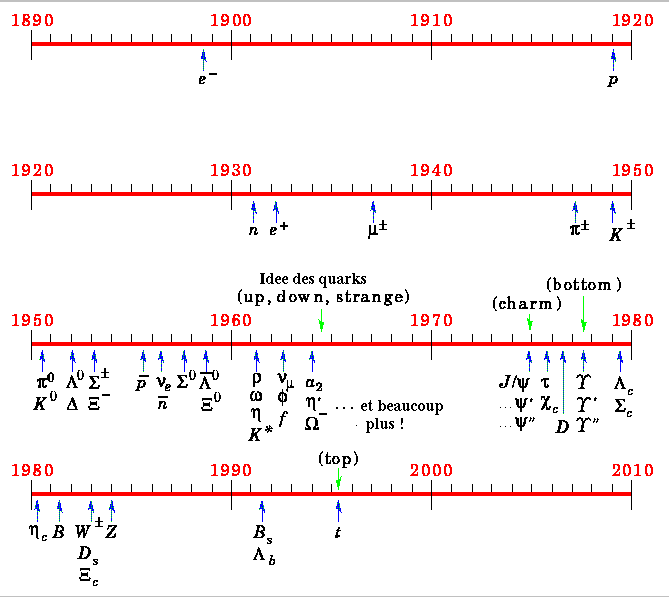
\includegraphics[width=11cm]{Chapter1/Discovery_timeline.png}
\caption{A timeline of particle discoveries.}
\label{fig:Discovery_timeline}
\end{center}
\end{figure}

The astonishing patterns observed in eightfold classification were signalling towards something striking. The explanation arrived in the form of ``Quark Model'',
proposed independently by Gell-Mann~\cite{GellMann:1964nj} and Zweig~\cite{Zweig:570209} in 1964.
They postulated that hadrons are not elementary but composed of fundamental entities, called ``quarks''.
These quarks are present in three flavours: $d$ (down), $u$ (up) and $s$ (strange). Each baryon is made up of three quarks while each meson is made up
of a quark and an anti-quark. Every member of the eightfold supermultiplets
got a quark substructure, however, the states like $\Delta^{++}$ ($uuu$), $\Delta^{-}$ ($ddd$) and $\Omega^{-}$ ($sss$) were appeared to violate the Pauli's exclusion
principle. A way out was proposed by O. W. Greenberg in the
same year by suggesting that each flavour quark further consists of three different color states (red, green and blue), known as color quantum number.
Quarks of different colors combined together in forming the hadrons and all the particles observed in nature are colorless.
This color hypothesis, though did not have any experimental proof, was able to describe the various aspects. 
Indirect searches which includes scattering of electrons with nuclear targets known as ``deep inelastic scattering''~\cite{dokshitzer1977calculation}
(similar to Rutherford's scattering of atom)
were performed in 1967 at SLAC and the first ever evidence of existence of proton substructure was observed.
The Yukawa's meson theory was not applicable for the strong force between quarks, so a new theory of strong force,
known as ``Quantum Chromodynamics'' (QCD) was developed in 1973 by H. Fritzsch and H. Leutwyler, along
with Gell-Mann~\cite{Fritzsch:1973pi}.
They proposed a gauge theory with SU(3) gauge group that predicted the existence of strong force carriers among quarks, termed as ``gluons''. The
first evidence of gluons was obtained at PETRA in 1979 in three-jet events~\cite{Gluons1979}. 

The elementary matter particles known at this stage were: four leptons ($e^{-}$, $\nu_{e}$, $\mu^{-}$, $\nu_{\mu}$) and three quarks ($u$, $d$, $s$).
The existence of a fourth quark, named as ``charm'' ($c$) quark, was predicted by Bjorken and Glashow around 1964~\cite{Bjorken:1964gz},
in order to maintain a symmetry between number of
quarks and leptons. In 1970, more technical aspects were provided for the existence of the charm quark by Glashow, Iliopoulos, and Maiani through GIM
mechanism~\cite{Glashow:1970gm}.
The first evidence of charm quark were obtained in 1974 in the form of $c\bar{c}$ ($J/\psi$) bound state simultaneously by C. C. Ting's
group at BNL~\cite{Aubert:1974js} and
B. Richter's group at SLAC~\cite{Augustin:1974xw}.\ The discovery of $J/\psi$ is known as $\textit{November Revolution}$ in the history.
The Glashow's symmetry that was restored
by the discovery of charm quark was soon broken in 1975 with the observation of a new lepton, known as ``tau'' ($\tau$) lepton,
by M. Perl et.\ al.\ at\ SLAC~\cite{Perl:1975bf}.\
This naturally led scientists to expect for a new family of quarks. Two years later, in 1977, a new heavy meson Upsilon ($\Upsilon$) was discovered by
L. Lederman et.\ al.\ at Fermilab~\cite{Herb:1977ek} and was immediately recognized as the bound state of fifth quark, named as bottom$/$beauty
($b$) quark. After the bottom
quark discovery, the search of its partner, named as truth$/$top ($t$) quark was very much anticipated. However, it took a really long time of 18 years to be finally
discovered in 1995 at Tevatron's CDF~\cite{Abe:1995hr} and D0~\cite{Abachi:1995iq} detectors at fermilab. 

The discovery of the strange particle $K^{+}$ was a startling one. On its first observation in 1947, it appeared to decay in two different
final states, initially thought as two different particles: $\tau^{+}$ (decaying into three $\pi$'s) and $\theta^{+}$ (decaying into two $\pi$'s).
The difference in masses and lifetimes of $\tau$ and $\theta$ were observed to be within experimental errors, but they had different parities~\cite{Lee:1956qn}.
Since parity was considered a universal symmetry then, it led to the famous $\tau$-$\theta$ puzzle
which was solved by the observation of parity violation in weak interactions
by C. S. Wu and collaborators in 1957~\cite{Wu:1957my}. The experimental verification of parity violation led 
to the reformulation of Fermi's theory of $\beta$ decay in terms of
Gamov-Teller transitions. Also, since Fermi's theory was only effective at low energies and found to violate unitarity at high energies, an attempt was
made to devise the theory in terms of intermediate vector particles acting as mediators. The first step was a proposal from C. N. Yang and R. Mills
who in 1954, developed the theory in terms of massless vector particles~\cite{Yang:1954ek}.
But weak interactions required its mediators to be massive, any attempt made to incorporate
masses led to the breaking of local gauge symmetry, thereby making the theory inconsistent. A complete description of weak
interactions was provided by S. Glashow~\cite{Glashow:1961tr}, A. Salam~\cite{Salam:1964ry} and S. Weinberg~\cite{Weinberg:1967tq} 
in terms of electroweak unification, by considering SU(2) $\times$ U(1) gauge group, having three weak gauge bosons denoted by $W^{\pm}$ and $Z$.
They invoked the Higgs mechanism proposed by Higgs~\cite{Higgs:1964ia, Higgs:1964pj, Higgs:1966ev}, Englert $\&$ Brout~\cite{Englert:1964et},
Guralnik, Kibble, $\&$ Hagen~\cite{Guralnik:1964eu} in 1964, that provided masses to gauge bosons by
spontaneous symmetry breaking of local gauge symmetries. The Higgs mechanism also predicted the existence of a new particle named Higgs boson, the mediator of Higgs field. 
The experimental verification of electroweak unification first arrived with the discovery of neutral currents by Gargamelle collaboration in 1973~\cite{Hasert:1973ff}
while performing neutrino scattering experiments, followed by the discovery of weak bosons, $W^{\pm}$~\cite{Arnison:1983rp, Banner:1983jy}
and $Z$~\cite{Arnison:1983mk, Arnison:1983zy, Bagnaia:1983zx} in $p\bar{p}$ collisions at SPS, CERN by UA1 and UA2
collaborations in 1983. The much awaited Higgs boson was finally discovered in 2012 by ATLAS~\cite{Aad:2012tfa} and CMS~\cite{Chatrchyan:2012xdj}
collaborations at CERN, thereby, verifying the source
of mass generation of universal particles. Both the collaborations has extensively studied the properties of this newly
found boson~\cite{CMS:yva, ATLAS:2014yka} and measured the mass to be $m_{H}$ $\approx$ 125 GeV$/$c$^{2}$ within experimental errors.


The SM of particle physics that incorporates six leptons ($e$, $\nu_{e}$, $\mu$, $\nu_{\mu}$, $\tau$, $\nu_{\tau}$),
six quarks ($u$, $d$, $s$, $c$, $b$, $t$) and three fundamental interactions (strong, EM, and weak) alongwith their carriers,
was developed in 1960s \nd\ 1970s. At present, all the particles
hypothesized by SM have been found and are well within the predictions.

\section{Standard Model}
The ``Standard Model'' is the theoretical model of particle physics that encapsulates the fundamental particles and their interactions to provide an ontological basis
to describe the organization of all matter forms except the ones related to gravity. The fundamental particles are classified into two categories:
the matter particles, known as ``fermions'', and the mediators of interactions, known as ``bosons''. In total, SM consists of 17 fundamentals including 12
fermions and 5 bosons. This model, over the years, has been found to be immensely successful in all of its experimental testings.
\subsection{Matter particles}
All the universal matter is made up of fermions, one set of fundamental particles. These fermions carry spin-$\frac{1}{2}$ and can be further
classified into leptons and quarks; each group consisting of six particles related in pairs, thereby forming three generations. 
%The most stable lightest particles form the first generation, with the higher generations formed by the heavier unstable particles.
%All the stable matter of the universe is made up of first generation particles; heavier particles of other generations eventually decay into the next lower generation.

The three quark generation involves: the up ($u$) and down ($d$) quarks, forming 1$^{st}$ generation, followed by the strange ($s$) and charm ($c$) quarks as 2$^{nd}$
generation and the top ($t$) and bottom ($b$) quarks as 3$^{rd}$ generation. These quarks carry fractional charges of $+\frac{2}{3}$e and $-\frac{1}{3}$e, e being the
electronic charge, and exhibit electromagnetic, strong as well as weak forces. Quarks also carry color charge, a property which does not allow them to exist freely
in nature. 

The three generation of leptons are: electron ($e$) and electron neutrino ($\nu_{e}$), muon ($\mu$) and muon neutrino ($\nu_{\mu}$), and tau ($\tau$)
and tau neutrino ($\nu_{\tau}$). Each lepton ($e$, $\mu$, $\tau$) carry one unit of negative charge while corresponding neutrinos are chargeless. SM predicts the
neutrinos to be massless, however, recent discoveries of neutrino oscillations~\cite{Fukuda:1998mi, Fukuda:2001nk, Ahmad:2002jz, Araki:2004mb, Aliu:2004sq, Michael:2006rx} assure that they have small non-zero mass. The leptons take part in electromagnetic and weak interactions while neutrinos involve in weak interactions only.
The three generations of quarks and leptons along with their crucial properties~\cite{Agashe:2014kda} are summarized in \tab{\ref{Table:SMparticles}}.
\begin{table}[h!]
\begin{center}
\resizebox{15cm}{!}{
%\begin{tabular}{c !{\vrule width -1pt}c !{\vrule width -1pt}c !{\vrule width -1pt}c !{\vrule width -1pt}c !{\vrule width -1pt}c !{\vrule width -1pt}c !{\vrule width -1pt}c}
\begin{tabular}{cccccccc}
\toprule
\belowrulesepcolor{Mygray}
\belowrulesepcolor{Mygray}
\belowrulesepcolor{Mygray}
\rowcolor{Mygray}[\dimexpr\tabcolsep+0.09pt\relax]
& \multicolumn{3}{c}{Leptons} & \phantom{abc} & \multicolumn{3}{c}{Quarks} \\
\aboverulesepcolor{Mygray}
\aboverulesepcolor{Mygray}
\aboverulesepcolor{Mygray}
%\arrayrulecolor{Mygray} \specialrule{0.1pt}{0pt}{-0.01pt} \arrayrulecolor{black} 
%\arrayrulecolor{Mygray}
%\cmidrule[0.1pt](r){1-1} \cmidrule[0.01pt](lr){5-5}
\rowcolor{Mygray}[\dimexpr\tabcolsep+0.09pt\relax]
& Flavor & Charge & Mass (MeV$/$C$^{2}$) && Flavor & Charge & Mass (MeV$/$C$^{2}$) \\
\aboverulesepcolor{Mygray}
\aboverulesepcolor{Mygray}
\aboverulesepcolor{Mygray}
\midrule
$1^{st}$ Generation \\
 & $e$ & -1 & 0.511 && $u$ & $+$\sfrac{2}{3} & $\sim2.2$ \\
 & $\nu_{e}$    &  0 & $<2.2\times10^{-6}$ && $d$ & $-$\sfrac{1}{3} & $\sim4.7$  \\
$2^{nd}$ Generation \\
 & $\mu$        & -1 & 105.7 && $c$ & $+$\sfrac{2}{3} & $\sim1.27\times10^{3}$  \\
 & $\nu_{\mu}$  &  0 & $<0.17$ && $s$ & $-$\sfrac{1}{3} & $\sim96$  \\
$3^{rd}$ Generation \\
 & $\tau$       & -1 & 1776.9 && $t$ & $+$\sfrac{2}{3} & $\sim173.21\times10^{3}$  \\
 & $\nu_{\tau}$ &  0 & $<18.2$ && $b$ & $-$\sfrac{1}{3} & $\sim4.18\times10^{3}$  \\
\bottomrule
\end{tabular}
}
\caption{Standard model fundamental fermion's three generations.}
\label{Table:SMparticles}
\end{center}
\end{table}
\vspace{-0.3in}

%%%%%%%%%%%%%%%%%%%%%%%%%%%%%%%%%%%%%%%%%%%%%%%%%%%%%%%%%%%%%%%%%%%%%%%%%%%%%%%%%%%%%%%%%%%%%%%%%%%%%%%%%%%%%%%%%%%%%%%%%%%%%%%%%%%%%%%%%%%%%%%%%%%
%% %---------------TABLE FOR MC samples-------------------                                                                                       %%
%% \definecolor{Gray}{gray}{0.9}                                                                                                                 %%
%% \begin{table}[h!]                                                                                                                             %%
%% \begin{center}                                                                                                                                %%
%% %\begin{ruledtabular}                                                                                                                         %%
%% \resizebox{16cm}{!}{                                                                                                                          %%
%% \begin{tabular}{@{}ccccccc@{}}                                                                                                                %%
%%   \hline                                                                                                                                      %%
%%   \rowcolor{Gray}                                                                                                                             %%
%%   &\multicolumn{3}{c||}{Leptons$\left(\text{spin}=\frac{1}{2}\right)$} & \multicolumn{3}{c|}{Quarks$\left(\text{spin}=\frac{1}{2}\right)$} \\ %%
%%   \cline{2-7}                                                                                                                                 %%
%% Generation & Flavor & Charge & Mass (MeV/c$^{2}$) &  Flavor & Charge & Mass (MeV/c$^{2}$) \\                                                  %%
%% \hline                                                                                                                                        %%
%%    & $e$          & -1 & 0.511               & $u$ & +2/3 & $\sim2.3$  \\                                                                     %%
%% 1  & $\nu_{e}$    &  0 & $<2.2\times10^{-6}$ & $d$ & -1/3 & $\sim4.8$  \\                                                                     %%
%% \hline                                                                                                                                        %%
%%    & $\mu$        & -1 & 105.7               & $c$ & +2/3 & $\sim1.27\times10^{3}$  \\                                                        %%
%% 2  & $\nu_{\mu}$  &  0 & $<0.17$             & $s$ & -1/3 & $\sim95$  \\                                                                      %%
%% \hline                                                                                                                                        %%
%%    & $\tau$       & -1 & 1777                & $t$ & +2/3 & $\sim173.21\times10^{3}$  \\                                                      %%
%% 3  & $\nu_{\tau}$ &  0 & $<15.5$             & $b$ & -1/3 & $\sim4.18\times10^{3}$  \\                                                        %%
%% \hline                                                                                                                                        %%
%% \end{tabular}                                                                                                                                 %%
%% }                                                                                                                                             %%
%% \caption{Three generation of elementary particles in the SM~\cite{Agashe:2014kda}.}                                                           %%
%% %\end{ruledtabular}                                                                                                                           %%
%%    \label{Table:SMparticles}                                                                                                                  %%
%% \end{center}                                                                                                                                  %%
%% \end{table}                                                                                                                                   %%
%%%%%%%%%%%%%%%%%%%%%%%%%%%%%%%%%%%%%%%%%%%%%%%%%%%%%%%%%%%%%%%%%%%%%%%%%%%%%%%%%%%%%%%%%%%%%%%%%%%%%%%%%%%%%%%%%%%%%%%%%%%%%%%%%%%%%%%%%%%%%%%%%%%

For each particle listed in table above, corresponding anti-particle having same mass and spin but opposite charge exists. 
\subsection{Forces and messenger particles}
All universal phenomena exhibit and experience four different kind of forces: strong, weak, electromagnetic and gravitational.
The gravity and electromagnetic interaction are the only two forces that can be experienced in day-to-day life.  
Strong and weak forces are applicable at sub-nuclear level only.
Standard model describes each force, except gravity, in the form of a physical theory, known as the Quantum Field Theory (QFT).
These theories are based on the analogy of exchange forces via mediators, the spin-1 bosons; another set of fundamental particles.
These mediators for electromagnetic interaction are ``photons'' whereas for strong force are ``gluons'' and for weak force are
``intermediate vector bosons'' $W^{\pm}$ and $Z$.  These forces operate between particles due to different charges: EM $\rightarrow$
electric charge, Strong $\rightarrow$ color charge, Weak $\rightarrow$ flavor charge. The \tab{\ref{Table:SMforces}} summarize the important
properties~\cite{Agashe:2014kda} of all the forces.

\begin{table}[h!]
\begin{center}
\resizebox{15cm}{!}{
%\begin{tabular}{c !{\vrule width -1pt}c !{\vrule width -1pt}c !{\vrule width -1pt}c !{\vrule width -1pt}c !{\vrule width -1pt}c !{\vrule width -1pt}c !{\vrule width -1pt}c}  %%% !{\vrule width -1pt} to make column line width less, so that white space not visible in colored table. but not working very nicely.
\begin{tabular}{cccccccc}
\toprule
\belowrulesepcolor{Mygray}
\belowrulesepcolor{Mygray}
\belowrulesepcolor{Mygray}
\rowcolor{Mygray}[\dimexpr\tabcolsep+0.09pt\relax]  
Force  & Mediator & Charge & Mass  & Range  & Rel.  & Long distance \\
\aboverulesepcolor{Mygray}
\aboverulesepcolor{Mygray}
\rowcolor{Mygray}[\dimexpr\tabcolsep+0.09pt\relax]
&          &        & (GeV$/$C$^{2}$) & (m) & Strength & behavior \\
\aboverulesepcolor{Mygray}
\aboverulesepcolor{Mygray}
\aboverulesepcolor{Mygray}
\midrule
Strong & Gluons ($g$) & 0 & 0   & $10^{-15}$ & 1 & $\sim$ r   \\
Electromagnetic & Photon ($\gamma$) & 0 & 0  & $\infty$ & $\sfrac{1}{137}$ & $\sfrac{1}{r^{2}}$ \\
Weak            & $W^{\pm}$  & $\pm1$ & 80.38 & $10^{-18}$ & $10^{-5}$  & $\sfrac{1}{r}e^{-mr}$  \\
                & $Z^{0}$    & 0      & 91.18 & & &  \\   
Gravity         & Graviton ($G$) & 0  & 0  & $\infty$ & $10^{-38}$ & $\sfrac{1}{r^{2}}$   \\
\bottomrule
\end{tabular}
}
\caption{Important properties of fundamental forces of universe.}
\label{Table:SMforces}
\end{center}
\end{table}
\vspace{-0.3in}


The electromagnetic interaction is the unification of electric and magnetic forces, first formulated in 1864 by Maxwell. The QFT of electromagnetic forces is known
as Quantum Electrodynamics (QED)~\cite{Feynman:1948ur, Feynman:1948km, Tomonaga:1948zz, Schwinger:1948iu, Schwinger:1948yk, Dyson:1949bp, Peskin:1995ev},
perfected by Feynman, Tomonaga, and Schwinger in the 1940s. EM interactions are of infinite range, thereby requiring its mediator (photon) to be massless.
The magnitude of this interaction is defined by means of a coupling constant,
$\alpha(Q^{2})= \frac{\alpha(\mu^{2})}{ 1 - \frac{\alpha(\mu^{2})}{3\pi}\text{log}\left(\frac{Q^{2}}{\mu^{2}}\right)}$
where $\mu$ is the typical scale of renormalization. The interaction strength increases with the increase of interaction energy and decrease of interaction length.

%\begin{equation}
%\alpha(Q^{2})= \frac{\alpha(\mu^{2})}{ 1 - \frac{\alpha(\mu^{2})}{3\pi}\text{log}\left(\frac{Q^{2}}{\mu^{2}}\right)},
%\label{eg:QEDalpha}
%\end{equation}

The weak force is answerable for existence of life on earth owing to its radioactive decays. It is actually the only force responsible for decay of particles.
It is also called Quantum Flavourdynamics (QFD) because of its capability of changing the flavour of quarks.
The first ever theory of weak forces was represented by Fermi in 1934;
later refined by Feynman and Gell-mann and finally, presented in its current scheme by Glashow, Weinberg, and Salam,
in 1960s~\cite{Glashow:1961tr, Salam:1964ry, Weinberg:1967tq}, in the form of Electroweak theory. This theory envision the unification of electromagnetic
and weak forces at some higher energy regime, thereby, predicting the existence of massive weak bosons, $W^{\pm}$ and $Z$.
The mechanism that is responsible for providing mass to weak bosons is known as Higgs mechanism that also predict the existence of one more fundamental boson called
Higgs boson. The magnitude of weak forces is found to depend on the coupling strength of weak bosons as well as their masses. 

The strong force is the mechanism responsible for the binding of quarks inside protons and neutrons, thereby, ensuring the stability of nucleus.
Most of the mass of a proton (or neutron) arises from the field energy provided by the strong force, the contribution of quark mass is almost negligible
in total proton's mass.
The field theory of strong force is known as Quantum Chromodynamics (QCD) that explains the interaction mechanism of strong force in the form of exchange of massless
gluons. The gluons interact with quarks as well as other gluons by means of a charge known as color charge. Color charge is analogous to electric charge 
but it comes in three different types. 
The behaviour of partons\footnote{Together quarks and gluons are referred to as partons} within the nucleons are determined by the properties of asymptotic
freedom and confinement. The coupling constant~\cite{Kluth:2006vf} determining the QCD interaction strength is given by,
\begin{equation}
\alpha_{s}(Q^{2})= \frac{12\pi}{(11\textrm{c}-2\textrm{n}_{\textrm{f}})\ln\left(\frac{Q^{2}}{\Lambda^{2}}\right)}
\label{eg:alpha_s}
\end{equation}
where $Q$ is the momentum transferred, c is the total number of quark colors (\ie 3), n$_{\textrm{f}}$ is the total number of quark flavors (\ie 6),
$\Lambda$ is the chromodynamics scale, which is given by:
\begin{equation}
\Lambda^{2}  = \mu^{2} \left[  \frac{-12\pi}{(11\textrm{c}-2\textrm{n}_{\textrm{f}}) \alpha_{s}(\mu^{2})  } \right]
\end{equation}
where $\mu$ is the renormalization scale. For $Q^{2}\to\infty$ and hence distance $\to0$, $\alpha_{s}(Q^{2})\to0$, which means that at high
energies with large momentum transfers in the interactions ($Q^{2}\gg\Lambda^{2}$), the coupling strength between the partons decreases, thereby making
the quarks and gluons to behave as free particles inside the nucleus. This property of quarks is referred to as
``asymptotic freedom''~\cite{Gross:1973ju,Gross:1974cs,Politzer:1974fr}.
For low $Q^{2}$, partons form hadronic bound states and can not be observed in isolated form. This attribute is referred to as ``quark confinement''. 


\subsection{SM as a gauge theory}
The standard model has been established on the notion of ``symmetry''. As per the statement of the Noether's theorm: the continuous symmetries of a system are
associated with conservation laws. For example, invariance of the laws of physics under space and time transformations, refer to as the symmetries of nature,
leads to the conservation of momentum and energy. These symmetry transformations of a system can be easily modelled in the form of
mathematical group representations, like the rotational symmetry of a system in n-dimension form the group representation for the special orthogonal group $SO (n)$.

A symmetry can be labelled as a global or local symmetry depending upon whether the transformation is same or different for each space-time point.
A physical theory of a system constructed by requiring local symmetries is known as ``gauge theory'', while the corresponding symmetry transformations
are called ``gauge transformations''.
The corresponding associated group representation is known as ``gauge group''. The gauge theory is called non-abelian if
the underlying gauge group is non-commutative. In SM, a physical system is described in terms of a Lagrangian which is then required to remain invariant
under a local gauge transformation. This requirement leads to the appearance of additional fields (known as ``gauge fields'') in the Lagrangian that
couples with the particles of the system, thereby generating the fundamental interactions. The number of gauge fields
in a gauge theory is determined by the dimension of the gauge group and the quanta of these gauge fields are known as the ``gauge bosons''.

The standard model portray the three fundamental forces in the form of gauge theories and unifies them as a non-abelian gauge theory under
$SU (3)_{color}$ $\otimes$ $SU (2)_{flavor}$ $\otimes$ $U (1)_{charge}$ gauge group. A more detailed description of this formalism is outlined as:

\subsubsection{Quantum electrodynamics}
Quantum electrodynamics is the abelian gauge theory of electromagnetic interactions characterized by the symmetry group $U (1)$.
The dynamics of a free particle of spin-$\frac{1}{2}$ can be represented in terms of Dirac Lagrangian,
\begin{equation}
\mathcal{L}_{\Psi} = \overline{\Psi}(x)(i\gamma^{\mu}\partial_{\mu} - m){\Psi}(x)
\label{eq:QEDLang}
\end{equation}
where $\Psi(x)$ is the Dirac field and $\gamma^{\mu}$ are the $4\times4$ Dirac matrices. We define a symmetry operation of the global phase transformations:
\begin{equation}
\Psi(x) \rightarrow \Psi^{\prime}(x) = e^{i{\alpha}}\Psi(x) \hspace{0.2 in}; \hspace{0.4 in} \overline{\Psi}(x) \rightarrow \overline{\Psi^{\prime}}(x) = e^{-i{\alpha}}\overline{\Psi}(x)
\label{eg:Globalphase}
\end{equation}
where phase $\alpha$ is independent of the spacetime variation. The Lagrangian remains invariant under this transformation, $\Delta\mathcal{L}$ = 0.
As per the statement of Noether's theorm, this invariance corresponds to a current $j^{\mu}$, known as Noether's current, defined by,
\begin{equation}
j^{\mu} = \frac{\partial\mathcal{L}}{\partial(\partial_{\mu}\Psi)}\delta\Psi \propto \overline{\Psi}\gamma^{\mu}{\Psi},
\label{eg:jmu}
\end{equation}
which remains conserved, that is, $\partial_{\mu}j^{\mu}$ = $0$. Now, if the phase is made to vary locally as a function of spacetime points, such that
\begin{equation}
\Psi(x) \rightarrow \Psi^{\prime}(x) = e^{i{\alpha}(x)}\Psi(x) \hspace{0.2 in}; \hspace{0.4 in} \overline{\Psi}(x) \rightarrow \overline{\Psi^{\prime}}(x) = e^{-i{\alpha}(x)}\overline{\Psi}(x)
\label{eg:Localphase}
\end{equation}
then under this symmetry operation, the Lagrangian transforms as:
\begin{equation}
\mathcal{L}_{\Psi} \rightarrow \mathcal{L}'_{\Psi} = \mathcal{L}_{\Psi} - \overline{\Psi}{\gamma}^{\mu}{\Psi}{\partial}_{\mu}{\alpha}(x) 
\label{eg:LangInLocalPhase}
\end{equation}
which is no longer invariant. In in attempt to achieve invariance, we introduce a covariant derivative $D_{\mu}$ and a new gauge field $A_{\mu}$ such as
\begin{equation}
\partial_{\mu} \rightarrow D_{\mu} = \partial_{\mu} - ieA_{\mu} \hspace{0.2 in} ; \hspace{0.4 in} A_{\mu} \rightarrow A^{\prime}_{\mu} = A_{\mu} + \frac{1}{e}\partial_{\mu}\alpha(x)
\label{eg:delToD}
\end{equation}
%\begin{equation}
%\label{eg:Amu}
%x\end{equation}
Under this transformation, the Lagrangian changed as
\begin{equation}
\begin{split}
  \mathcal{L}_{\Psi} \rightarrow \mathcal{L}^{\prime}_{\Psi} & = \overline{\Psi^{\prime}}(i\gamma^{\mu}D_{\mu} - m){\Psi^{\prime}} \\
  & = \overline{\Psi}e^{-i\alpha(x)}(i\gamma^{\mu}(\partial_{\mu} - ieA^{\prime}_{\mu}) - m)e^{i\alpha(x)}{\Psi} \\
  & = \overline{\Psi}e^{-i\alpha(x)}(i\gamma^{\mu}\partial_{\mu} + e\gamma^{\mu}(A_{\mu} + \frac{1}{e}\partial_{\mu}\alpha(x)) - m)e^{i\alpha(x)}{\Psi} \\
  & = \overline{\Psi}(i\gamma^{\mu}\partial_{\mu} - m){\Psi} + e\overline{\Psi}\gamma^{\mu}A_{\mu}{\Psi} \\
  & = \mathcal{L}_{\Psi} + e\overline{\Psi}\gamma^{\mu}A_{\mu}{\Psi}
  \label{eg:newLang}
\end{split}
\end{equation}
which is invariant under the local gauge transformation defined in \eqn{\ref{eg:Localphase}}.

Demanding local gauge invariance under the gauge group $U (1)$ has resulted into the introduction of gauge field $A_{\mu}$ which is none other than the required
electromagnetic field, also called the photon field, and it couples with Dirac particles ($e^{-}$s) through the term $e\overline{\Psi}\gamma^{\mu}A_{\mu}{\Psi}$. Since $A_{\mu}$ is a physical field, we
must introduce a gauge invariant kinetic energy term for this, given by 
\begin{equation}
  \mathcal{L}_{K.E.} = -\frac{1}{4}F^{\mu\nu}F_{\mu\nu}
  \label{eg:Lke}
\end{equation}
where $F_{\mu\nu}$ = $\partial_{\mu}A_{\nu} - \partial_{\nu}A_{\mu}$, known as the electromagnetic strength tensor. Adding this term, the complete gauge invariant
Lagrangian for electromagnetic interactions can be written as:
\begin{equation}
  \begin{split}
  & \mathcal{L}_{total} = \mathcal{L}_{free} + \mathcal{L}_{int} + \mathcal{L}_{K.E} \\
  & \mathcal{L}_{total} = \overline{\Psi}(i\gamma^{\mu}\partial_{\mu} - m){\Psi} + e\overline{\Psi}\gamma^{\mu}A_{\mu}{\Psi} - \frac{1}{4}F^{\mu\nu}F_{\mu\nu}
    \label{eg:Lcomp}
    \end{split}
\end{equation}

If a mass term, like $m^{2}A_{\mu}A^{\mu}$, is considered for field $A_{\mu}$, it will again spoil the gauge invariance. So this term is prohibited in the QED
Lagrangian and corresponding gauge particle, the photon, remain massless. The interaction term in the Lagrangian, $e\overline{\Psi}\gamma^{\mu}A_{\mu}{\Psi}$ can
also be written as $-j^{\mu}A_{\mu}$ where $j^{\mu}$ = $-e\overline{\Psi}\gamma^{\mu}{\Psi}$, known as the current density, $-e$ being the electric charge.
The current density $j^{\mu}$ is a conserved quantity of electromagnetic interactions.

\subsubsection{Electroweak}
The electroweak theory is a unified theory of electromagnetic and weak interactions. This theory came into existence in an attempt to derive a self-consistent
invariant gauge theory for weak interactions, analogous to QED.\ The weak interactions were first proposed by Fermi in 1934 as an explanation
of $\beta$-decay. He came up with the following interaction Lagrangian for $\beta$-decay process:
\begin{equation}
\mathcal{L}_{w} = G_{F}(\overline{\Psi}_{p}\gamma_{\mu}{\Psi}_{n})(\overline{\Psi}_{e}\gamma^{\mu}{\Psi}_{\nu})
\end{equation}
where $G_{F}$ is the Fermi coupling constant and ${\Psi}_{p}$, ${\Psi}_{n}$, ${\Psi}_{e}$, ${\Psi}_{\nu}$ are the particle fields.
In his proposal, Fermi considered the interaction of four fermions at one point, known as contact interaction. The most remarkable difference in Fermi Lagrangian
was the presence of charged currents, contrary to neutral current of QED.\

The observation of parity violation in weak interactions emphasized that weak interactions involve only left-handed fermions and right-handed anti-fermions
(observed experimentally in 1958 by Goldhaber et.\ al.~\cite{Goldhaber:1958nb}) and led to the introduction of axial-vector terms in the Fermi Lagrangian,
\begin{equation}
\mathcal{L}_{w} = \frac{G_{F}}{\sqrt{2}}(\overline{\Psi}_{p}\gamma_{\mu}(1 - g_{A}\gamma_{5}){\Psi}_{n})(\overline{\Psi}_{e}\gamma^{\mu}(1 - \gamma_{5}){\Psi}_{\nu})
\end{equation}
where $g_{A}$ = $|\frac{G_{A}}{G_{V}}|$, $G_{V}$ and $G_{A}$ being the constants for vector and axial-vector couplings respectively.
%In the formation of this Lagrangian, the projection operators, $P_{L}$ = $\frac{1 - \gamma^{5}}{2}$ and $P_{R}$ = $\frac{1 + \gamma^{5}}{2}$ were introduced
%having the properties: $P^{2}_{L} = P_{L}$, $P^{2}_{R} = P_{R}$, $P_{L}P_{R} = 0$ and $\gamma^{\mu}P_{L} = P_{R}\gamma^{\mu}$.
%Their operation on the fermionic fields, $P_{L}\Psi$ = $\Psi_{L}$ ($\overline{\Psi}P_{L}$ = $\overline{\Psi}_{R}$) and
%$P_{R}\Psi$ = $\Psi_{R}$ ($\overline{\Psi}P_{R}$ = $\overline{\Psi}_{L}$), results into left and right projections. The importance of these projection operators can be
%considered from the fact that
%\begin{equation}                                                                                                                           
%\begin{split}                                                                                                                              
%  \overline{\Psi}_{e}\gamma^{\mu}\left(\frac{1 - \gamma_{5}}{2}\right){\Psi}_{\nu} & = \overline{\Psi}_{e}\gamma^{\mu}P_{L}{\Psi}_{\nu}  
%  = \overline{\Psi}_{e}\gamma^{\mu}P^{2}_{L}{\Psi}_{\nu}  %(using the property, P^{2}_{L} = P_{L})\\                                    
%  = \overline{\Psi}_{e}P_{R}\gamma^{\mu}P_{L}{\Psi}_{\nu}  %(using, \gamma^{\mu}\gamma^{5} = -\gamma^{5}\gamma^{\mu})\\                 
%  = \overline{\Psi}_{eL}\gamma^{\mu}{\Psi}_{{\nu}L} %(using, \overline{\Psi}P_{R} = \overline{\Psi_{L}})\\                              
%\label{eg:projection}                                                                                                                      
%\end{split}                                                                                                                                
%\end{equation}                                                                                                                             
%implying that only left-handed fermions experience weak interactions.
However, this $V - A$ theory was still incomplete in the sense that
it could not be renormalized and violated unitarity at high energies.

Later on, in 1960s, it was observed independently by Glashow, Salam and Weinberg~\cite{Glashow:1961tr, Salam:1964ry, Weinberg:1967tq}
that a gauge-invariant theory for the weak interactions can be constructed if electromagnetic interactions are also included under the gauge group
${SU(2)}_{L} \times {U(1)}_{Y}$. The group ${SU(2)}_{L}$, where $L$ refers to left-handed,
forms the gauge group of weak interactions and considers the doublet of left-handed lepton (or an up-type quark)
and lepton neutrino (or a down-type quark) as its fundamental representation under the weak isospin, $T$ = $\frac{1}{2}$,
which remains conserved under this group transformation.
The group ${U(1)}_{Y}$ form the gauge group under the weak hypercharge, $Y$.  
The weak isospin's $3^{rd}$ component, $T_{3}$
and weak hypercharge, $Y$ are related to the electric charge, $Q$ by the Gell-Mann-Nishijima relation~\cite{Nakano:1953zz, Nishijima:1955zz, Gell-Mann:1956iqa}:
$Q = T_{3} + \frac{Y}{2}$. The \tab{\ref{tab:EWK_fermions}} summarize the electroweak singlets and doublets and the various quantum numbers associated with them.

%\begingroup\setlength{\fboxsep}{0pt}
%\colorbox{lightgray}{%
\begin{table}[h]
\begin{center}
\resizebox{11.5cm}{!}{    
\begin{tabular}{ccccccc}
\toprule
\belowrulesepcolor{Mygray}
\belowrulesepcolor{Mygray}
\belowrulesepcolor{Mygray}
\rowcolor{Mygray}[\dimexpr\tabcolsep+0.09pt\relax]
 \multicolumn{3}{c}{Fermions: Singlets \& Doublets} & $Q$ & $T$ & $T_{3}$ & $Y$ \\
\aboverulesepcolor{Mygray}
\aboverulesepcolor{Mygray}
\aboverulesepcolor{Mygray}
\midrule
%\rowcolor{black!20}
$                    
\left(               
\begin{array}{c}     
{\nu}_{e}\\          
e^{-}\\              
\end{array}          
\right)_{L}          
$ &                  
$                    
\left(               
\begin{array}{c}     
{\nu}_{\mu}\\        
{\mu}^{-}\\          
\end{array}          
\right)_{L}          
$ &                  
$                    
\left(               
\begin{array}{c}     
{\nu}_{\tau}\\       
{\tau}^{-}\\         
\end{array}          
\right)_{L}          
$ &                  
$                    
\begin{array}{c}     
0\\                  
-1\\                 
\end{array}          
$ &                  
$                    
\begin{array}{c}     
\sfrac{1}{2}\\                
\sfrac{1}{2}\\                
\end{array}          
$ &                  
$                    
\begin{array}{c}     
\sfrac{1}{2}\\                
-\sfrac{1}{2}\\               
\end{array}          
$ &                  
$                    
\begin{array}{c}     
-1\\                 
-1\\                 
\end{array}          
$ \\                 
\\                   
$                    
\left(               
\begin{array}{c}     
u\\                  
d\\                  
\end{array}          
\right)_{L}          
$ &                  
$                    
\left(               
\begin{array}{c}     
c\\                  
s\\                  
\end{array}          
\right)_{L}          
$ &                  
$                    
\left(               
\begin{array}{c}     
t\\                  
b\\                  
\end{array}          
\right)_{L}          
$ &                  
$                    
\begin{array}{c}     
\sfrac{2}{3}\\                
-\sfrac{1}{3}\\               
\end{array}          
$ &                  
$                    
\begin{array}{c}     
\sfrac{1}{2}\\                
\sfrac{1}{2}\\                
\end{array}          
$ &                  
$                    
\begin{array}{c}     
\sfrac{1}{2}\\                
-\sfrac{1}{2}\\               
\end{array}          
$ &                  
$                    
\begin{array}{c}     
\sfrac{1}{3}\\                
\sfrac{1}{3}\\                
\end{array}          
$ \\                 
\\
$e_{R}$ & $\mu_{R}$ & $\tau_{R}$ & $-1$ & $0$ & $0$ & $-2$ \\
$u_{R}$ & $c_{R}$ & $t_{R}$ & $\sfrac{2}{3}$ & $0$ & $0$ & $\sfrac{4}{3}$ \\
$d_{R}$ & $s_{R}$ & $b_{R}$ & $-\sfrac{1}{3}$ & $0$ & $0$ & $-\sfrac{2}{3}$ \\
\bottomrule
\end{tabular}
}
\caption{Assignment of the various quantum numbers including $T_{3}$ and $Y$ to the electroweak singlet and doublet fundamental fermions.}
\label{tab:EWK_fermions}
\end{center}
\end{table}


\vspace{-0.2in}
If we consider only the first generation quarks and leptons, then
\begin{equation}
\Psi_{L} = 
\left(
\begin{array}{c}
\nu_{e^{-}}\\
e^{-}\\
\end{array}
\right)_{L}
\hspace{0.2cm} or \hspace{0.2cm}\left(
\begin{array}{c}
u \\
d \\
\end{array}
\right)_{L}
\hspace{0.3cm}; \hspace{0.4cm} \Psi_{R} = e^{-}_{R}, \hspace{0.1cm} u_{R}, \hspace{0.1cm} d_{R}
\end{equation}
form the left-handed and right-handed particle fields. The free particle Lagrangian for these fields can be written as,
\begin{equation}
\mathcal{L}_{free} = \overline{\Psi}_{L}(i\gamma^{\mu}\partial_{\mu} - m){\Psi}_{L} + \overline{\Psi}_{R}(i\gamma^{\mu}\partial_{\mu} - m){\Psi}_{R}
\label{eg:EWfree}
\end{equation}
which remains invariant under the following global gauge transformations:
\begin{equation}
  \begin{split}
   \Psi_{L} \rightarrow \Psi^{\prime}_{L} = e^{i{\alpha_{a}}T^{a}+i{\beta}\frac{Y}{2}}{\Psi_{L}} \hspace{0.2 in} ; \hspace{0.4 in} 
  %\overline{\Psi}_{L} \rightarrow \overline{\Psi^{\prime}}_{L} = e^{-i{\alpha_{a}}T^{a}-i{\beta}Y}\overline{\Psi}_{L} \\
   \Psi_{R} \rightarrow \Psi^{\prime}_{R} = e^{i{\beta}\frac{Y}{2}}{\Psi_{R}} %\hspace{0.56in} ; \hspace{0.4 in} 
  %\overline{\Psi}_{R} \rightarrow \overline{\Psi^{\prime}}_{R} = e^{-i{\beta}Y}\overline{\Psi}_{R}
  \label{eg:EWKGlobalphase}
  \end{split}
\end{equation}
where $T_a$ and $Y$ are the generators of $SU(2)$ and $U(1)$ transformations with $T_a$ = $\sigma_{a}/2$,
$\sigma_{a}$ are the Pauli spin matrices\footnote{Pauli matrices are a set of three 
$2\times2$ hermitian and unitary complex matrices, given as:
\newline
$\sigma_{1} = \left(\begin{array}{cc} 0 & 1 \\ 1 & 0 \end{array}\right),\:\:\:
\sigma_{2} = \left(\begin{array}{cc} 0 & -i \\ i & 0 \end{array}\right),\:\:\:
\sigma_{3} = \left(\begin{array}{cc} 1 & 0 \\ 0 & -1 \end{array}\right).$}
for $a$ = 1,2,3. However, the invariance
of Lagrangian is carried away when the phases $\alpha$ and $\beta$ are made to vary as a function of spacetime points. In order to restore the invariance,
the following covariant derivatives and fields are introduced:
\begin{equation}
  \begin{split}
    & \partial_{\mu} \rightarrow D_{\mu} = \partial_{\mu} - igT_{a}W_{\mu}^{a} - ig^{\prime}\frac{Y}{2}B_{\mu} & & \textrm{for SU(2) doublets}\\
    & \partial_{\mu} \rightarrow D_{\mu} = \partial_{\mu} - ig^{\prime}\frac{Y}{2}B_{\mu} & & \textrm{for U(1) singlets}
    \label{eg:EWKdelToD}
    \end{split}
\end{equation}
where the fields $W_{\mu}$ and $B_{\mu}$ varies as
\begin{equation}
W_{\mu} \rightarrow W^{\prime}_{\mu} = W_{\mu} + \frac{1}{g}\partial_{\mu}\alpha(x) - \alpha(x) \times W_{\mu} \hspace{0.2in} ; \hspace{0.4in} B_{\mu} \rightarrow B^{\prime}_{\mu} = B_{\mu} + \frac{1}{g^{\prime}}\partial_{\mu}\beta(x) 
\label{eg:EWKfields}
\end{equation}
Under these covariant transformations, the Lagrangian achieve invariance as:
\begin{equation}
\begin{split}
  \mathcal{L}_{free} \rightarrow \mathcal{L}^{\prime}_{free} = \mathcal{L}_{fermion} & = \mathcal{L}_{free} + g\overline{\Psi}_{L}\gamma^{\mu}T_{a}W_{\mu}^{a}{\Psi_{L}} + g^{\prime}\frac{Y}{2}B_{\mu}(\overline{\Psi}_{L}\gamma^{\mu}{\Psi_{L}} + \overline{\Psi}_{R}\gamma^{\mu}{\Psi_{R}}) \\
  & = \mathcal{L}_{free} + g\overline{\Psi}_{L}\gamma^{\mu}T_{a}W_{\mu}^{a}{\Psi_{L}} + g^{\prime}\overline{\Psi}\gamma^{\mu}\frac{Y}{2}B_{\mu}{\Psi} \\
  & = \overline{\Psi}_{L}(i\gamma^{\mu}D_{\mu} - m){\Psi}_{L} + \overline{\Psi}_{R}(i\gamma^{\mu}D_{\mu} - m){\Psi}_{R}
  \label{eg:newLang}
\end{split}
\end{equation}
where $T_{a}W_{\mu}^{a}$ = $\frac{\sigma_{a}}{2}.W_{\mu}^{a}$ = $\frac{1}{2}(\sigma_{1}W_{\mu}^{1} + \sigma_{2}W_{\mu}^{2} + \sigma_{3}W_{\mu}^{3})$. Replacing the 
Pauli matrices with the matrix form, and using $W_{\mu}^{\pm}$ = $(W_{\mu}^{1} \mp iW_{\mu}^{2})/{\sqrt{2}}$,  
\begin{equation}
  \begin{split}
     T_{a}W_{\mu}^{a} = \frac{1}{2}\left(\begin{array}{lr} W_{\mu}^{3}  &W_{\mu}^{1} - iW_{\mu}^{2} \\ W_{\mu}^{1} + iW_{\mu}^{2}  & -W_{\mu}^{3} \end{array} \right) =
    \frac{1}{2}\left(\begin{array}{lr} W_{\mu}^{3}  &\sqrt{2}W_{\mu}^{+} \\ \sqrt{2}W_{\mu}^{-} & -W_{\mu}^{3} \end{array} \right)
\label{eg:Wmus}
\end{split} 
\end{equation}

Thus, the invariance under local gauge transformations led to the introduction of four gauge bosons into the theory: a positively charged $W^{{\mu}+}$,
a negatively charged $W^{{\mu}-}$ and two neutrals $W^{{\mu}3}$, and $B^{\mu}$ where $W_{\mu}$'s interacts with only the left-handed fermions while $B_{\mu}$
interacts with both left and right handed. The kinetic energy terms for the gauge fields can be written as,
\begin{equation}
  \begin{split}
    & \mathcal{L}_{K.E.} = -\frac{1}{4}W^{{\mu\nu}a}W_{\mu\nu}^{a} -\frac{1}{4}B^{\mu\nu}B_{\mu\nu} & & \textrm{where,} \\
    & W^{a}_{\mu\nu} = \partial_{\mu}W_{\nu}^{a} - \partial_{\nu}W_{\mu}^{a} -g\epsilon_{abc}W_{\mu}^{b}W_{\nu}^{c}, & & \epsilon_{abc} \textrm{ is totally anti-symmetric tensor}\\
    & B_{\mu\nu} = \partial_{\mu}B_{\nu} - \partial_{\nu}B_{\mu}
    \label{eg:EWK_Lke}
    \end{split}
\end{equation}
The corresponding weak current densities that will remain conserved under $SU(2)$ $\times$ $U(1)$ are represented as:
\begin{equation}
  \begin{split}
    & j_{\mu}^{T} = -g\overline{\Psi}_{L}\gamma_{\mu}T{\Psi}_{L} \hspace{0.2in} ; \hspace{0.4in} j_{\mu}^{Y} = -g^{\prime}\overline{\Psi}\gamma_{\mu}Y{\Psi}
    \label{eg:EWK_jmu}
  \end{split}
\end{equation}
Using the general form of electromagnetic current, $j_{\mu}^{em} = -e\overline{\Psi}\gamma_{\mu}Q{\Psi}$, where $Q$ is the charge operator for EM
interactions, and Gell-Mann-Nishijima relation, $Q = T_{3} + \frac{Y}{2}$,
\begin{equation}
  \begin{split}
    & j_{\mu}^{em} = j_{\mu}^{3} + \frac{j_{\mu}^{Y}}{2}
    \label{eg:EWK_jmu_all}
  \end{split}
\end{equation}
Thus, the electromagnetic current is a combination of weak isospin and weak hypercharge current. Likewise, the two neutral physical gauge fields,
$Z^{\mu}$ and $A^{\mu}$ are the orthogonal combinations of gauge fields $W^{{\mu}3}$ and $B^{\mu}$ with a mixing angle $\theta_{W}$, \\
\begin{minipage}{0.55\textwidth}
\begin{equation}
  \begin{split}
    & Z^{\mu} = W^{{\mu}3}\cos{\theta}_{W} - B^{\mu} \sin{\theta}_{W} \\
    & A^{\mu} = W^{{\mu}3}\sin{\theta}_{W} + B^{\mu} \cos{\theta}_{W}
    \label{eq:EWK_Zmu_Amu}
\end{split}
\end{equation}
\end{minipage}%
\hfill
\begin{minipage}{0.35\textwidth}
  \begin{figure}[H]
    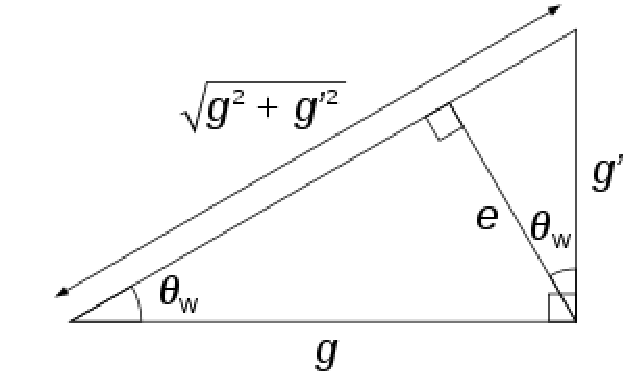
\includegraphics[width=5cm]{Chapter1/Weinberg_angle_relation_between_coupling_constants.pdf}
    \caption{\label{fig:Weinberg_angle} $W^{{\mu}3}$-$B^{\mu}$ plane}
  \end{figure}
\end{minipage}

\noindent obtained by considering a plane in $W_{\mu}^{3}-B_{\mu}$ with $W_{\mu}^{3}$ along x-axis and $B_{\mu}$ along y-axis. The relation among
$\theta_{W}$, $g$ and $g^{\prime}$ is obtained as 
\begin{equation}
  \begin{split}
& \cos{\theta_{W}} = \frac{g}{\sqrt{g^{2} + g^{{\prime}2}}} \hspace{0.2in} ; \hspace{0.2in} \sin{\theta_{W}} = \frac{g^{\prime}}{\sqrt{g^{2} + g^{{\prime}2}}}
  \label{eg:theta_w}
  \end{split}
\end{equation}
Also, using \eqn{\ref{eg:EWK_jmu_all}}, the following relation between $e$, $g$ and $g^{\prime}$ holds,
\begin{equation}
e = g\sin{\theta_{W}} = g^{\prime}\cos{\theta_{W}}
\label{eg:e_g_gprime}
\end{equation}

Thus, the gauge invariance has been restored, but no required mass term appears for the gauge bosons.
Any mass term like $m^{2}W^{\mu}W_{\mu}$ will break the gauge invariance. This hints towards an underlying mechanism,
which provide the masses to gauge bosons alongwith keeping the theory renormalizable and gauge invariant. This mechanism is
known as Higgs mechanism~\cite{Higgs:1964ia, Higgs:1964pj, Higgs:1966ev, Englert:1964et, Guralnik:1964eu}.

\noindent
\underline{\bf{Higgs mechanism:}} The higgs mechanism to endow the gauge bosons with mass has been developed on the idea of
``spontaneous symmetry breaking''~\cite{Djouadi:2005gi} which considers the breaking of a symmetry of a physical system such that
the underlying laws remains invariant under the symmetry transformation, but the physical system itself changes. It is a spontaneous
action that changes the system from a symmetrical state to an asymmetrical state.  

To realize this, a complex scalar field Lagrangian, gauge invariant under $SU(2)$ $\times$ $U(1)$ has been introduced into the electroweak theory
using the same covariant derivative defined in
\eqn{\ref{eg:EWKdelToD}}.
\begin{equation}
\mathcal{L}_{\Phi} = {(D_{\mu}\Phi)}^{\dag}D^{\mu}\Phi - \mu^{2}\Phi^{\dag}\Phi - \lambda{(\Phi^{\dag}\Phi)}^{2}
\label{eq:HiggsLag}
\end{equation}
where $\Phi$ is a $SU(2)$ $\times$ $U(1)$ multiplet of complex scalar fields having weak isospin, $T$ = $1/2$ and weak hypercharge, Y = 1:
\begin{equation}
\Phi = \left(\begin{array}{c} \phi^{+} \\ \phi^{0} \end{array}\right) = \frac{1}{\sqrt{2}} 
 \left(\begin{array}{c} \phi_{1} + i\phi_{2} \\ \phi_{3} + i\phi_{4}  \end{array}\right)
\end{equation}
The potential term of the Lagrangian, $V(\Phi)$ = $\mu^{2}\Phi^{\dag}\Phi + \lambda{(\Phi^{\dag}\Phi)}^{2}$ has two parameters, $\mu^{2}$ and $\lambda$, that
decide its nature. The four particle coupling $\lambda$ specifies the self interactions among the $\phi$ fields and is always positive. We have two
choices for $\mu^{2}$: $\mu^{2}$ $>$ $0$ and $\mu^{2}$ $<$ $0$. For positive $\mu^{2}$, $V(\Phi)$ has a minimum at $\Phi$ = $0$ and the Lagrangian describes
the QED interaction among scalar particles, but for negative $\mu^{2}$,
the potential behaves differently with ground state exhibited by, $\Phi^{\dag}\Phi$ = $\frac{-\mu^{2}}{2\lambda}$ = $\frac{v^{2}}{2}$, in a multi-dimensional regime.
The corresponding potential for real scalar fields before and after symmetry breaking is presented in \fig{\ref{fig:Higgs_potential}}.

Choosing one particular minimum will break the symmetry spontaneously. We choose a ground state where $\phi_{3}$ = $v$, $\phi_{1}$ = $\phi_{2}$ = $\phi_{4}$ = 0 so that
\begin{equation}
\Phi =\frac{1}{\sqrt{2}}\left(\begin{array}{c} 0 \\ v \end{array}\right), \:\:\: \textrm{with } v =\frac{\mu}{\sqrt{\lambda}}
\end{equation}

\begin{figure}[htpb]
\centerline{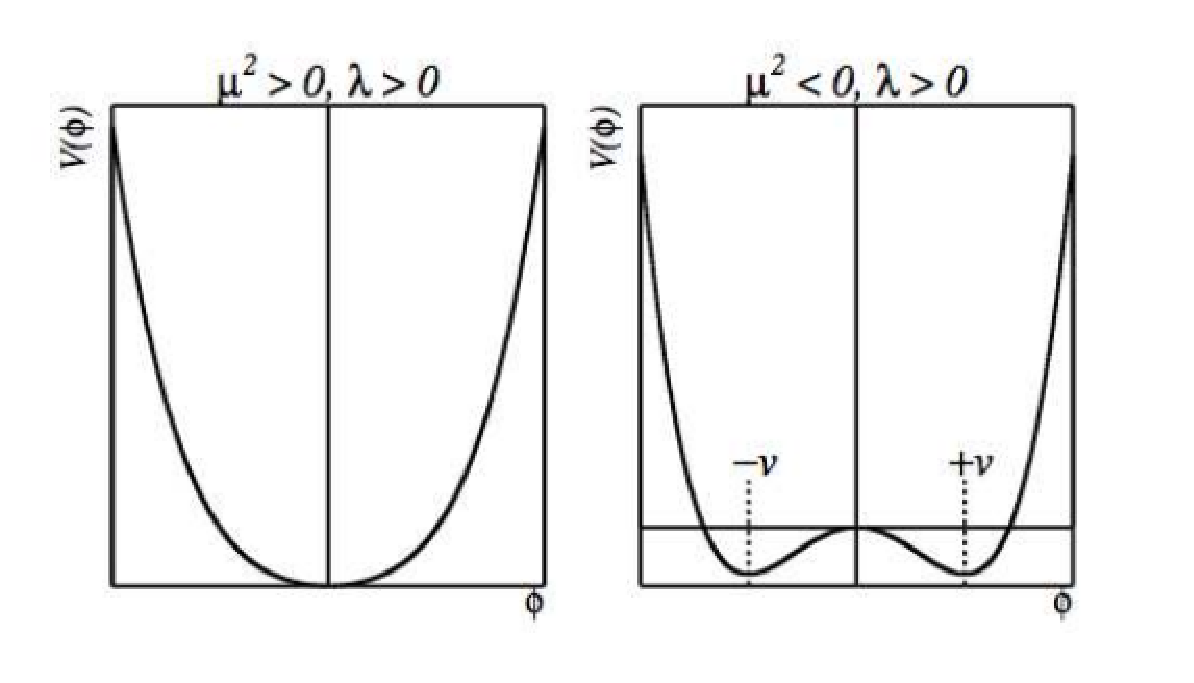
\includegraphics[width=11cm]{Chapter1/Higgs_potential.pdf}}
\caption{A potential with real scalar field $V(\phi)$ = $\mu^{2}\phi^{2}$ + $\lambda{\phi^{4}}$ before and after spontaneous symmetry breaking.}
\label{fig:Higgs_potential}
\end{figure}
\vspace{0.1in}

\noindent This particular choice will break both $SU(2)_{L}$ and $U(1)_{Y}$ gauge symmetries but maintain the $U(1)_{em}$ gauge symmetry. Thus the vacuum state remain invariant
under $U(1)_{em}$ and photon does not acquire any mass. We perturb this field by considering small quantum fluctuations $h(x)$, $h_{1}(x)$, $h_{2}(x)$ and $h_{4}(x)$
corresponding to $\phi_{3}$, $\phi_{1}$, $\phi_{2}$ and $\phi_{4}$ fields respectively, such that
\begin{equation}
  \Phi(x) = \frac{1}{\sqrt{2}} \left(\begin{array}{c} h_{1}(x) + i h_{2}(x) \\ v + h(x) + i h_{4}(x) \end{array}\right)
  \label{eq:Higgs_phi_final}
\end{equation}
Substituting this value of $\Phi$ in the Lagrangian and using the relations defined in \eqns{\ref{eq:EWK_Zmu_Amu},~\ref{eg:theta_w}} and~\ref{eg:e_g_gprime} results into,
\begin{equation}
  \mathcal{L}_{\Phi} = \frac{1}{2}(\partial_{\mu}h)^{2}  + \frac{1}{4}g^{2}(v+h)^{2}(W^{{\mu}+}W_{-}^{\mu}) + \frac{1}{8}(g^{2} + g^{{\prime}2})(v+h)^{2}Z^{\mu}Z_{\mu}
                       - {\lambda}v^{2}h^{2} - {\lambda}vh^{3} - \frac{{\lambda}h^{4}}{4} + \frac{{\lambda}v^{4}}{4}
\end{equation}
This Lagrangian consists of gauge invariant massive higgs field $h$ with mass, $m_{h}$ = $\sqrt{2{\lambda}v^{2}}$, along with the mass terms
for weak gauge bosons $W_{\mu}^{\pm}$ and $Z_{\mu}$. It can be seen that there is no mass term for photon field $A_{\mu}$.
\begin{equation}
  M_{W^{\pm}} = \frac{1}{2}gv, \hspace{0.2in} M_{Z} = \frac{1}{2}v{\sqrt{g^{2} + g^{{\prime}2}}}; \hspace{0.2in} M_{A} = 0 
\end{equation}
Thus, the spontaneous breaking of gauge symmetry has resulted into the generation of masses of weak gauge bosons. The other terms of the Lagrangian represents
the interaction terms of the higgs field with gauge bosons. The same higgs field also provide the masses to fermions through Yukawa coupling defined by,
\clearpage
\begin{equation}
  \mathcal{L}_{Yukawa} = -y_{l}\bar{L}{\phi}e_{R} -y_{u}\bar{Q}(-i{\sigma}_{2}){\phi}^{\ast}u_{R} -y_{d}\bar{Q}{\phi}d_{R} + h.c.
  \label{eq:Yukawa_coup}
\end{equation}
with $y_{l,u,d}$ being Yukawa coupling constants and ${u}_{R}$, ${d}_{R}$ (${e}_{R}$) being the left-handed doublet and right-handed singlet quark (lepton) fields.
Now again we break the symmetry and perturb the system around the minima to obtain a value for field $\Phi$ defined in \eqn{\ref{eq:Higgs_phi_final}}. Using it in the
Lagrangian gives,
\begin{equation}
  \mathcal{L}_{Yukawa} = -\frac{1}{\sqrt{2}}y_{l}\bar{l}_{L}(v+h)l_{R} -\frac{1}{\sqrt{2}}y_{q}\bar{q}_{L}(v+h)q_{R},
\end{equation}
where $l_{L,R}$ and $q_{L,R}$ denote the lepton and quark fields. We see that a mass term for fermions appears in this lagrangian given by, $m_{f}$ = $\frac{1}{\sqrt{2}}y_{f}v$, showing that the coupling strength $y_{f}$ of fermions with higgs field is
proportional to the mass of fermion. 

Thus, the full electroweak Lagrangian is a sum of four terms,
\begin{equation}
  \mathcal{L}_{EWK} = \mathcal{L}_{fermion} + \mathcal{L}_{K.E.} + \mathcal{L}_{\Phi} + \mathcal{L}_{Yukawa}
\end{equation}
 
\subsubsection{Quantum chromodynamics}
The theory of strong force, known as Quantum chromodynamics, has also been developed on the steps of QED. Since quarks come in three colors, in contrast to the single
charge of QED photon, the gauge group considered is SU(3), an extension of $U(1)$ gauge group in 3-dimension. It is a non-abelian gauge theory
with quark's color fields forming the fundamental representation. The Lagrangian for free quark fields can be written as,
\begin{equation}
\mathcal{L}_{q} = \sum_{j = 1,2,3} \overline{q}_{j}(x)(i\gamma^{\mu}\partial_{\mu} - m){q_{j}}(x)
\label{eq:QCDLang}
\end{equation}
This Lagrangian is conserved under the global phase transformation with the conserved currents, $j_{\mu}^{c}$ = $\sum_{j = 1,2,3} g\overline{q}_{j}\gamma^{\mu}T_{a}q_{j}$,
known as color charge densities. Considering the invariance of Lagrangian under the local gauge transformations,
\begin{equation}
q_{j}(x) \rightarrow q_{j}^{\prime}(x) = e^{i{\alpha}_{a}(x)T_{a}}q_{j}(x) 
\label{eg:QCDLocalphase}
\end{equation}
where $T_{a}$, $a$ = $1,2,\ldots,8$ are the generators of $SU(3)$ transformations with $[T_{a}, T_{b}]$ = $if_{abc}T_{c}$, $f_{abc}$ are anti-symmetric
real structure constants. To make Lagrangian invariant under this local phase, we introduce the 
following covariant derivatives and fields,
\begin{equation}
  D_{\mu} = \partial_{\mu} + igT_{a}G_{\mu}^{a} \hspace{0.2 in} ; \hspace{0.4 in} G_{\mu}^{a} \rightarrow G_{\mu}^{a} - \frac{1}{g}\partial_{\mu}\alpha_{a}(x) -
  f_{abc}\alpha_{b}(x)G_{\mu}^{c} 
\label{eg:QCDdelToD}
\end{equation}
where last term of $G_{\mu}^{a}$ signifies the non-abelian nature of the theory. Substituting $\partial_{\mu}$ $\rightarrow$ $D_{\mu}$ in the Lagrangian,
\begin{equation}
\mathcal{L}_{q} \rightarrow \mathcal{L}'_{q} = \mathcal{L}_{q} - \sum_{j = 1,2,3} g\overline{q}_{j}\gamma^{\mu}T_{a}G_{\mu}^{a}{q_{j}} 
  \label{eq:QCDLang_Dmu}
\end{equation}
Also, considering the kinetic energy term for the gauge fields, $G_{\mu}^{a}$, we can write the complete QCD Lagrangian as,
\begin{equation}
  \mathcal{L}_{q} = \sum_{j = 1,2,3} \overline{q}_{j}(x)(i\gamma^{\mu}\partial_{\mu} - m){q_{j}}(x) - g\overline{q}_{j}\gamma^{\mu}T_{a}G_{\mu}^{a}{q_{j}} -
  \frac{1}{4}G_{\mu\nu}^{a}G^{{\mu\nu}a}
  \label{eq:QCDLang_final}
\end{equation}
where,
\begin{equation}
  G_{\mu\nu}^{a} = \partial_{\mu}G_{\nu}^{a} - \partial_{\nu}G_{\mu}^{a} - gf_{abc}G_{\mu}^{b}G_{\nu}^{c}
  \label{eq:Gmunu_QCD}
\end{equation}

Thus, we can see that the invariance of Lagrangian under local gauge has resulted into the appearance of interaction fields into the theory with the mediators
of interaction, gluons, remaining massless.

%%%%%%%%%%%%%%%%%%%%%%%%%%%%%%%%%%%%%%%%%%%%%%%%%%%%%%%%%%%%%%%%%%%%%%%%%%%%%%%%%%%%%%%%%%%%%%%%%%%%%%%%%%%%%%%%%%%%%%%%%%%%%%%%%%%%%%%%%%%%%%%%%%%%%%%%%%%%%%%%%%%%%%%%%%
%% \subsubsection{Grand unification theory}                                                                                                                             %%
%% The standard model predicts the existence of a unified theory of electroweak and strong interactions, known as Grand Unified Theory (GUT).                           %%
%% The grand unification is believed to have existed at very high energies at the beginning of the universe. This theory unifies the three fundamental forces into one  %%
%% under a grand unified gauge group $\mathcal{G}$,                                                                                                                     %%
%% \begin{equation}                                                                                                                                                     %%
%%   SU (3)_{C} \times SU (2)_{L} \times U (1)_{Y} \subset \mathcal{G}                                                                                                  %%
%%   \label{eq:GUT}                                                                                                                                                     %%
%% \end{equation}                                                                                                                                                       %%
%% where the gauge transformations in $\mathcal{G}$ relate the couplings $g$ and $g^{\prime}$ of electroweak interaction to the strong coupling $\alpha_{s}$.           %%
%% All the three interactions are then interpreted by a single gauge group $\mathcal{G}$ and single coupling $g_{\mathcal{G}}$,                                         %%
%% with $g_{\mathcal{G}}$ relating to $g$, $g^{\prime}$ and $\alpha_{s}$ in some specific ways.                                                                         %%
%% However, an exact form of the grand unification group $\mathcal{G}$ and corresponding symmetries are yet to be found out.                                            %%
%% One of the predictions of the GUTs is the decay of protons. Since no proton decays has been observed yet, it ruled out the existence of simple GUTs, like $SU(5)$ or %%
%% $SO(10)$.                                                                                                                                                            %%
%%                                                                                                                                                                      %%
%% Also, there is no quantized theory of gravitation yet, still a Theory of Everything (TOE) unites the theory of quantum gravity and GUT as well                       %%
%% into one common framework.                                                                                                                                           %%
%%%%%%%%%%%%%%%%%%%%%%%%%%%%%%%%%%%%%%%%%%%%%%%%%%%%%%%%%%%%%%%%%%%%%%%%%%%%%%%%%%%%%%%%%%%%%%%%%%%%%%%%%%%%%%%%%%%%%%%%%%%%%%%%%%%%%%%%%%%%%%%%%%%%%%%%%%%%%%%%%%%%%%%%%%

\subsection{Challenges faced by SM:\ unknown mysteries}
The standard model is acknowledged to be the most successful theoretical model till today. Over the years, it has been built up owing to the lively
conversations between theoretical predictions and experimental proofs. Even after being able to describe so many natural phenomena, this model is not
considered perfect. The reason being several existing questions that standard model can not adequately explain. Some of these include:
\vspace{-0.15in}
\begin{itemize}
   \setlength\itemsep{0.03em}
\item {\bf{Gravity}}: Standard model does not include gravity and provides no explanation for it.
\item {\bf{Three generations}}: No particular justification has been given in SM as to why only three particle generations exist and why there is so much variation
  in masses of particles from different generations.
\item {\bf{Neutrino mass}}: In SM, neutrinos are regarded as massless. However, there are many experimental
  results~\cite{Fukuda:2001nk, Fukuda:1998mi, Araki:2004mb, Aliu:2004sq} which prove that neutrinos have small tiny non-zero mass.
\item {\bf{Matter-Antimatter asymmetry}}: The imbalance of matter and anti-matter within the observable universe, also referred to as baryon asymmetry,
  has been one of the greatest mysteries of particle physics for which standard model has no answer.
\item {\bf{Dark energy and dark matter}}: It has been observed in various cosmological observations that the visible matter accounts for only 5$\%$ of the total
  energy-mass content of the universe. The SM gives no explanation for the rest of about 25$\%$ of the non-luminous dark matter and about 70$\%$ of dark energy.   
\item {\bf{Short range of strong force}}: Usually, the range of a force is inversely proportional to the mass of its mediator. But this is not true for
  strong force. Its mediators, gluons are massless, still, this force is of limited range. No explanation for this is provided in SM. 
\end{itemize}
\vspace{-0.2in}
So the picture depicted by SM is not perfect, it has been, therefore, regarded as a piece of a bigger picture that will be explained by
some beyond the standard model theories. 

\section{Beyond The Standard Model}
Many theoretical models have been developed to overcome the deficiencies observed in standard model. These models are collectively known as ``Beyond the Standard Model''
(BSM) theories. The most famous among these are String theory, Supersymmetry, Technicolor, compositeness etc.
\subsection{Model of excited quarks}
The study represented in this thesis is based on a model that considers the excited state of quarks ($\qstar$) and leptons ($\lstar$),
also known as compositeness models~\cite{Pati:1975md, Eichten:1983hw, Baur:1987ga, Baur:1989kv}.
The prime motivation for these models are the presence of three quark and lepton generations with similar properties. This replication points toward
some underlying structure identical in all the families. The most implicit signature of this sub-structure is the observation of a fermion (quark or lepton)
in the excited state. The analogy with excited states has been made on the basis of a very basic physics phenomena. We know that a composite system,
e.g.\ a hydrogen atom, consists of various energy levels arising due to the interactions among its constituents. Thus, the
observation of a system in excited state is the confirmation of its composite structure.
The excited state of fermions is assumed as a resonance state which then eventually decay into SM particles. 

The fundamental particles that quarks and leptons are considered to be composed of, are known as ``preons''. These preons are postulated to experience a new kind of
force that becomes very strong at a particular scale $\Lambda$, known as the compositeness scale, forming quarks and leptons bound states. 
Excited quarks and leptons can interact with their ordinary counterparts through contact interactions for $\Lambda$ $>>$ $\sqrt{\shat}$ and through gauge
mediation for $\Lambda$ $<$ $\sqrt{\shat}$ where $\sqrt{\shat}$ is the center of mass energy. The model used in this study assumes compositeness scale $\Lambda$
$<$ $\sqrt{\shat}$ and mass scale of excited quarks $M_{\qstar}$ = $\Lambda$, gauge interactions dominate over contact interactions in this regime.
The excited quark model used in this study~\cite{Baur:1989kv} considers a $SU(3)$ $\times$ $SU(2)$ $\times$ $U(1)$ symmetry with ground state quarks in the
form of left-handed doublets and right-handed singlets while the excited quarks in the form of left- and right-handed doublets. 
\begin{equation}
\textrm{Ground state: }\left(\begin{array}{c} u \\ d \\ \end{array} \right)_{L}
\hspace{0.1cm}, \hspace{0.1cm} u_{R}, \hspace{0.1cm} d_{R} \hspace{0.5in}
\textrm{Excited state: }\left(\begin{array}{c} \ustar \\ \dstar \\ \end{array} \right)_{L}
\hspace{0.1cm}, \hspace{0.1cm} \left(\begin{array}{c} \ustar \\ \dstar \\ \end{array} \right)_{R}
\end{equation}
The excited quarks interact with gauge bosons via vectorlike coupling defined by the Lagrangian:
\begin{equation}
\mathcal{L}_{gauge} = \bar{q^{\star}}\gamma^{\mu} \left[ g_{s}\frac{\lambda^{a}}{2}G_{\mu}^{a} + g\frac{\tau^{b}}{2}W_{\mu}^{b} + g'\frac{Y}{2}B_{\mu} \right]q^{\star}
\end{equation}
where $g_{s}$, $g$, and $g^{\prime}$ are the coupling constants for strong and electroweak interactions; $G_{\mu}^{a}$, $W_{\mu}$, and $B_{\mu}$ denote
the gauge fields corresponding to $SU(3)$, $SU(2)$, and $U(1)$ gauge groups. The excited quarks attain spin and isospin value of $\frac{1}{2}$ and weak hypercharge
$Y$ value of $\frac{1}{3}$ under this model. The gauge interaction mediated between ordinary and excited quarks by gauge bosons is obtained through the
requirement of gauge invariance and is of magnetic-moment type, defined by the effective Lagrangian:
\begin{equation}
{\mathcal L}_{int} = \frac{1}{2\,\Lambda}\bar{q^{\ast}_{R}} \, \sigma^{\mu\nu}
\left[g_{s}f_{s}\frac{\lambda^{a}}{2}G^{a}_{\mu\nu}\;+\;gf\frac{\tau^{b}}{2}W_{\mu\nu}^{b}\;+\;g'f'\frac{Y}{2}B_{\mu\nu} \right] q_{L} + h.c.,
\label{eq:Lagrangian1}
\end{equation}
Here $G^{a}_{\mu\nu}$, $W_{\mu\nu}$, and $B_{\mu\nu}$ are corresponding field-strength tensors while $\lambda_{a}$, $\tau_{b}$, $Y$
are the corresponding generators for $SU(3)$, $SU(2)$, and $U(1)$ fields. The constants $f_{s}$, $f$, $f'$ determine the strength of a coupling and are
evaluated using the compositeness dynamics, these are considered to be equal to unity to allow for the standard model like coupling strengths. 

A composite quark can acquire an excited state by the absorption of a gluon and will radiate a photon, gluon or weak boson on returning to the ground state.
The branching fractions of excited quark decays into various final states is given in the \tab{\ref{Table:qstarBR}} below.
%---------------TABLE FOR MC samples-------------------
\begin{table}[h!]
\begin{center}
%\begin{ruledtabular} 
  %\resizebox{7cm}{!}{
\renewcommand{\arraystretch}{1.2}
\begin{tabular}{lr}
\toprule
\belowrulesepcolor{Mygray}
\belowrulesepcolor{Mygray}
\belowrulesepcolor{Mygray}
\rowcolor{Mygray}[\dimexpr\tabcolsep+0.09pt\relax]
Decay Channel \hspace{0.5in}      & BR     \\
\aboverulesepcolor{Mygray}
\aboverulesepcolor{Mygray}
\aboverulesepcolor{Mygray}
\midrule
$\qstar\to$qg       \hspace{0.5in} & $\sim$ 83\% \\
$\qstar\to$q$\gamma$\hspace{0.5in} & $\sim$ 2\%  \\
$\qstar\to$q$Z^{0}$ \hspace{0.5in} & $\sim$ 5\%  \\
$\qstar\to$q$W^{-}$ \hspace{0.5in} & $\sim$ 10\%  \\
\bottomrule
\end{tabular}
%}
\caption{Approximate estimate of branching fractions (BR) of \qstar\ decay in different channels, assumptions made are: $\Lambda$ = $M_{\qstar}$ and $f$ = $f^{\prime}$ = $f_{s}$.}
%\end{ruledtabular}
\label{Table:qstarBR}
\end{center}
\end{table}
%\vspace{-0.3in}

\vspace{-0.3in}

This study considers an excited light ($\ustar,\dstar$) and heavy ($\bstar$) flavor quark decaying into a quark and a photon final state.
The physics processes contributing to this final state are represented in the form of Feynman diagrams in the \fig{\ref{fig:qstarSig}}
with $q$ referring to $u, d$ and $b$ quark.
%\vspace{-0.2in}
\begin{figure}[h]
\begin{center}
\subfloat[qg fusion]{\label{fig:qgFusion}\includegraphics[width=4.6cm]{Chapter1/Feynman_diagrams/Signal_qgFusion.pdf}}
\hspace{0.1 in}
\subfloat[q$\bar{\textrm{q}}$ annihilation]{\label{fig:qqbarAnni}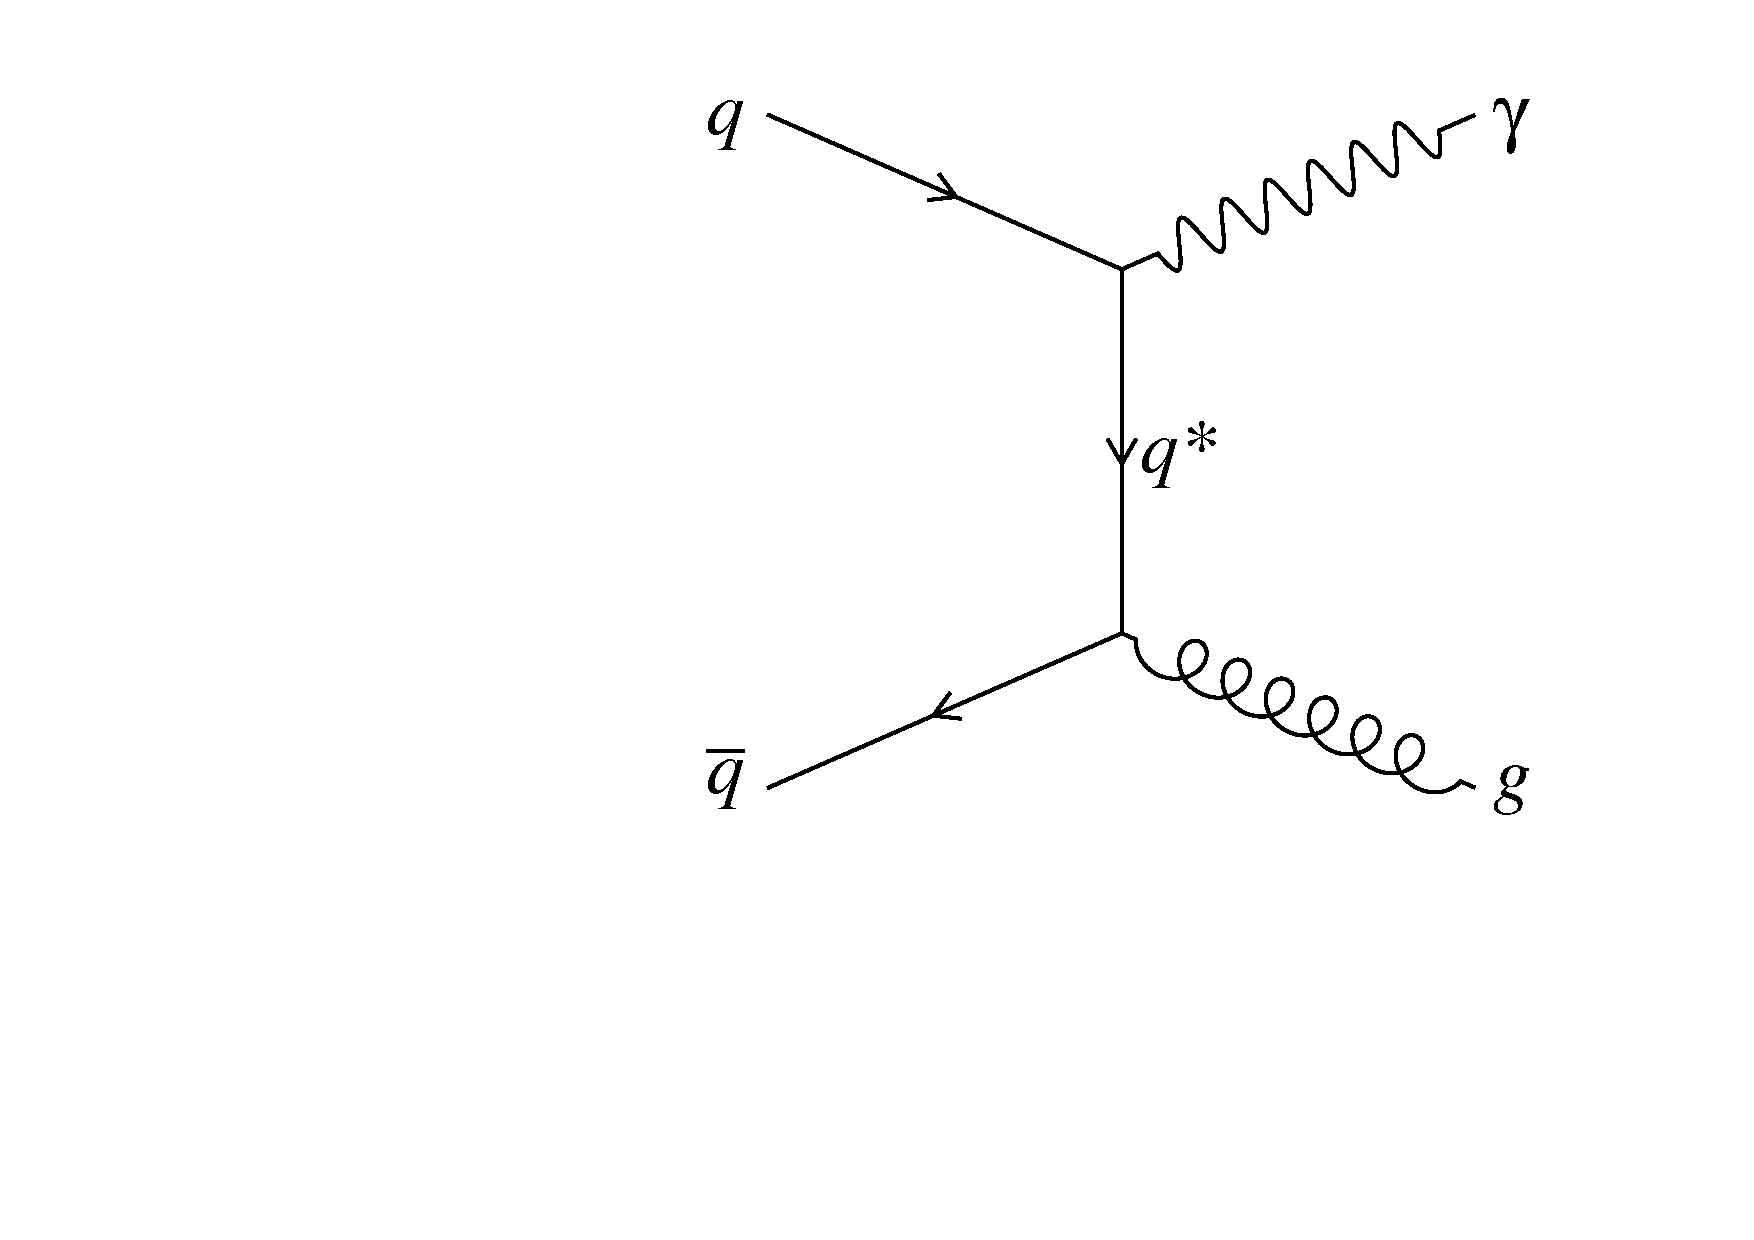
\includegraphics[width=4.4cm]{Chapter1/Feynman_diagrams/Signal_qqbarAnnihilation.pdf}}
\hspace{0.1 in}
\subfloat[gg fusion]{\label{fig:ggFusion}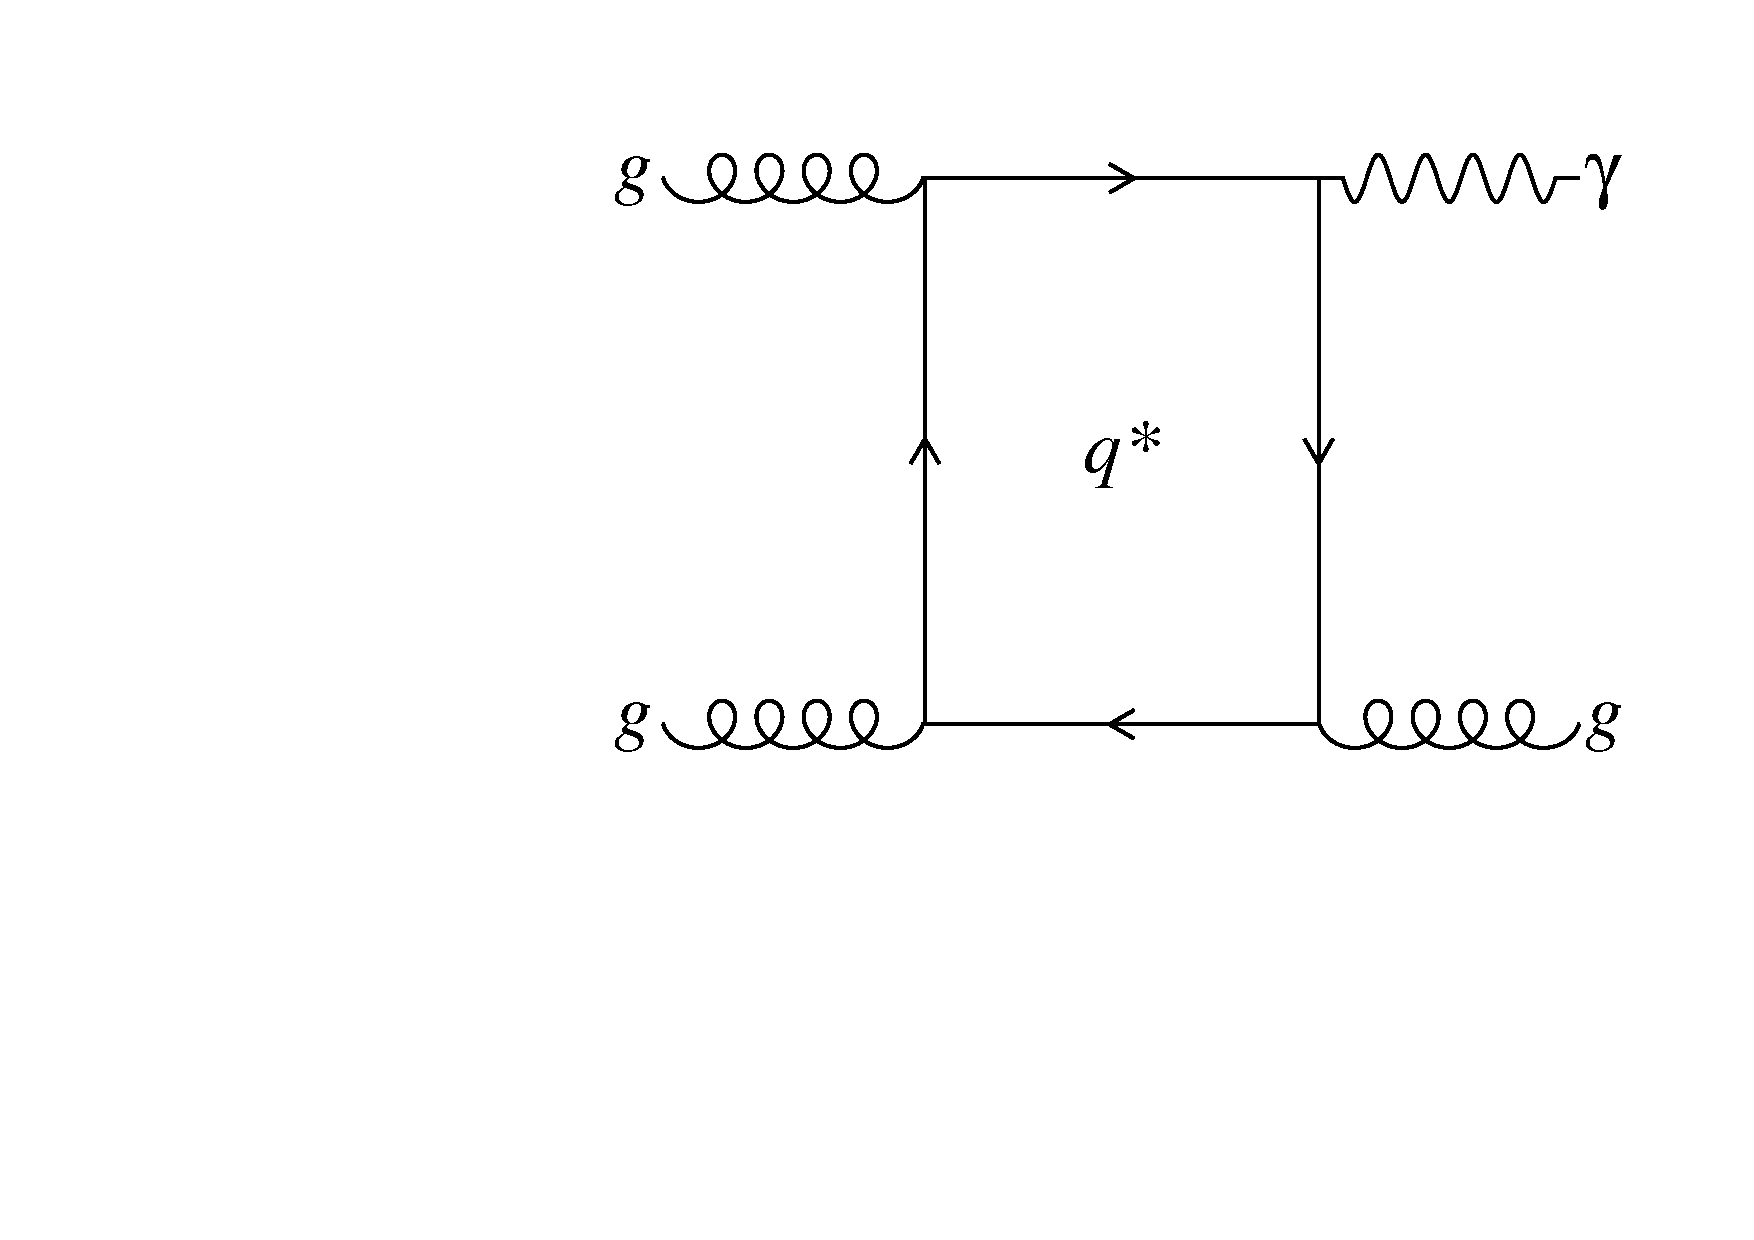
\includegraphics[width=4.4cm]{Chapter1/Feynman_diagrams/Signal_ggFusion.pdf}}
\caption{Feynman diagrams for $\qstar$ $\rightarrow$ $\gamma$ + jet final state with (a) quark-gluon fusion (b) quark-antiquark annihilation
  (c) gluon-gluon fusion processes. Whereas the light quarks will show their presence in all the three modes, heavy bottom quark will appear only in quark-gluon fusion and quark-antiquark annihilation.}
\label{fig:qstarSig}
\end{center}
\end{figure}
\vspace{-0.3in}

Under the assumption $\Lambda$ $<$ $\sqrt{\shat}$, gauge interactions will be dominating and the excited quarks will be produced mainly via the
s-channel\footnote{s,t and u are called Mandelstam variables. For a $2-2$ scattering process
  of initial momenta p$_{1}$ and p$_{2}$ and final momenta p$_{3}$ and p$_{4}$, the variables are defined as, s = (p$_{1}$ + p$_{2}$)$^{2}$ = (p$_{3}$ + p$_{4}$)$^{2}$,
  t = (p$_{1}$ $-$ p$_{3}$)$^{2}$ = (p$_{4}$ $-$ p$_{2}$)$^{2}$ and u = (p$_{1}$ $-$ p$_{4}$)$^{2}$ = (p$_{3}$ $-$ p$_{2}$)$^{2}$. Each one represents a different
  Feynman diagram of a process.}
quark-gluon fusion process. The scattering of an ordinary quark and gluon in s-channel
will produce an excited quark resonance that will tower over the continuous SM $\gamjet$ background. Appearance of excited quark in other channels will be
captured in the form of excess of events over the background distribution. 

\subsection{A follow-up of previous searches}
Many attempts have been made in the past to look for the evidences of quark compositeness. But no success has been gained yet.
A summary of the various experiments that deployed their potential in this important search are reported here. 

The ZEUS detector at HERA looked for excited quarks of heavy flavor in $e^{+}p$ collisions at $\sqrt{s}$ = 300\unit{GeV} and excluded the excited quarks
in the mass range 40-169\unit{GeV} at the 95$\%$ confidence level (CL)~\cite{Breitweg:1997qa}. 

The CDF detector collaboration at Tevatron also searched for excited quarks in \gamjet\ and
dijet channels in $\textrm{p}\bar{\textrm{p}}$ collisions at center of mass
energy of 1.8 TeV and excluded the ranges $80<\mqstar<540\unit{GeV}$~\cite{CDFexclgj}, $200<\mqstar<520\unit{GeV}$ \nd\
$580<\mqstar<760\unit{GeV}$~\cite{CDFexcljj}, respectively. The D0 collaboration at Tevatron looked for evidence in dijet final state~\cite{D0excl}
and excluded $M_{\qstar}$ below 775\unit{GeV} at 95\% CL.\ The CMS and ATLAS Collaborations have also performed the searches in $\textrm{pp}$ collisions
at $\sqrt{s}$ = 7\unit{TeV}, 8 \unit{TeV} as well as 13\unit{TeV}. At $\sqrt{s}$ = 8\unit{TeV}, exclusions have been reported by both the collaborations
in different channels. At $\sqrt{s}$ = 13\unit{TeV}, ATLAS had excluded $\qstar$ below 5.2\unit{TeV}
with 95$\%$ CL in the dijet channel~\cite{ATLAS:2015nsi} and below 4.4\unit{TeV} in the $\gamjet$ channel~\cite{Aad:2015ywd}. The CMS Collaboration
has also excluded excited quarks below 5.0\unit{TeV} in the dijet channel~\cite{Khachatryan:2015dcf}.

Searches for excited states of heavy bottom quarks have also been performed earlier in different channels.
The ATLAS collaboration searched for $\bstar$ in $tW$ final state at $\sqrt{s}$ = 7\unit{TeV}~\cite{Aad:2013rna} and excluded $M_{\bstar}$ for masses below 870\unit{GeV}.
The CMS collaboration have looked for excited b-quarks in $tW$ and dijet final state at $\sqrt{s}$ = 8\unit{TeV}. In $tW$ final state, it excluded
$\bstar$ upto the masses of 1.53\unit{TeV} for vector-like couplings~\cite{Khachatryan:2015mta} at 95$\%$ CL while in
dijet final state, it claimed an exclusion in the range of
1.20-1.56\unit{TeV}~\cite{Khachatryan:2015sja}. At $\sqrt{s}$ = 13\unit{TeV}, no search for $\bstar$ has been performed yet, this study, therefore, presents the
first search for $\bstar$ at $\sqrt{s}$ = 13\unit{TeV}. 


%\section{Thesis Organization}



%keywords that can be used at any place: turbulence, intellectual, retrospect (a survey of past few years), thence (as a consequence),
  


\clearemptydoublepage
\chapter{The Experimental Apparatus}
The ``Large Hadron Collider'' (LHC) accelerator and the ``Compact Muon Solenoid'' (CMS) detector, situated across Swiss-French border in Geneva, Switzerland
at the European Organization of Nuclear Research (CERN), has been used to accumulate data for this study. This chapter presents a brief introduction and
description of the design and performance of these accelerator and detector facilities.

\section{The Large Hadron Collider}
The Big-Bang theory~\cite{Gorbunov:2011zz} provides an explanation of the origin of the universe. It says that the universe initially started from a small singularity
and an explosion (called Big-Bang) put the universe into a continuous state of inflation, so it took around 13.7 billion years for the universe to reach in the
present state (\fig{\ref{fig:BigBang}}).
During the initial seconds after the birth of universe, the temperature was tremendously high and the universe consists of plasma of vast number
of fundamental particles interacting with each other with extremely high energies. In order to study the properties of early universe,
scientists use particle accelerators in which sub-atomic particles travelling at relativistic speeds are made to undergo inelastic collisions to reproduce the
conditions that existed at the time of Big-Bang or soon there after.

\begin{figure}[h]
\begin{center}
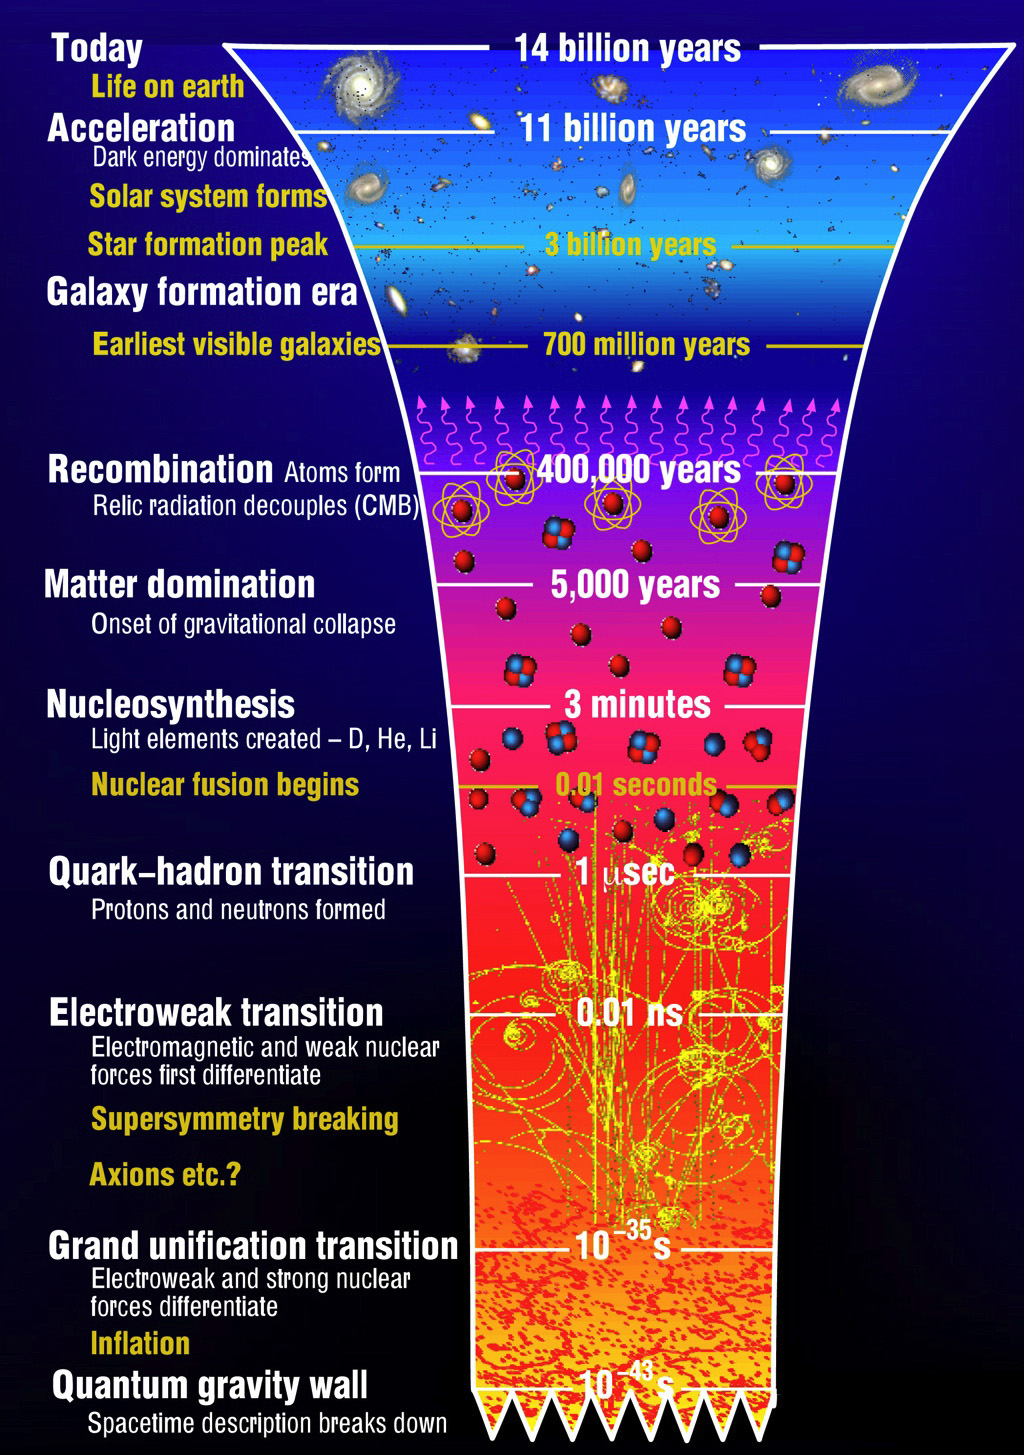
\includegraphics[width=8cm]{Chapter2/big_bang_timeline.png}
\caption{Big-Bang timeline.}
\label{fig:BigBang}
\end{center}
\end{figure}

The Large Hadron Collider~\cite{Bruning:782076, Evans:2008zzb} as the name suggests is a large circular accelerator having a circumference of $\sim$ 27\unit{km}
which accelerates counter rotating beams of hadrons and collides them to study the fundamental properties and interactions of quarks, leptons and bosons.  
It is the world's largest and most complex particle accelerator ever built. Earlier particle accelerators like ``Large Electron Positron'' collider
(LEP)~\cite{LEP} at CERN (in the same tunnel where LHC has been built) and Tevatron~\cite{Holmes:2011ey} at Fermilab, Batavia, IL, USA,
have been extensively used to confirm the predictions and test the precision of Standard Model parameters. Both of these were circular colliders.
The LEP was an $e^{+}e^{-}$ collider with a center of mass energy ($\sqrt{s}$) ranging from 90\unit{GeV} to 209\unit{GeV}
while Tevatron was a $\textrm{p}\bar{\textrm{p}}$ collider with $\sqrt{s}$ $=$ 1.8\unit{TeV} and 1.96\unit{TeV}.   
Studying a collision data obtained from electron-positron beam is far more easier as compared to proton beams due to the absence of hadronic background in the former.
However, in a circular ring of a particular radius, the loss of energy caused by synchrotron radiations is given as:
\begin{equation}
  -\Delta{E} = \frac{4{\pi}{\alpha}}{3r}\beta^{3}\gamma^{4} \:\:\: (\beta = v/c \simeq 1 \:\: \textrm{and} \:\: \gamma = E/mc^{2} \:\: \textrm{for relativistic speeds}),
  \label{eq:synchro}
\end{equation}
which is very large due to small mass of $e^{+}$ and $e^{-}$ and further increases as the speed $v$ approaches the speed of light $c$.
The choice is to either increase the radius of the circular rings or to use linear colliders or use heavy
particles in collision beams. The first two instances are not very easy to meet either due to technical or financial constraints,
so in order to achieve very high energies, proton beams are used. Since $m_{p}$ $\simeq$ $2000\:m_{e}$, use of proton beam reduces
synchrotron losses by a factor of ${(2000)}^{4}$ $\simeq$ $10^{13}$.

The requirement of very high energies for particle accelerators can be explained by the fact that in scattering experiments, the wavelength
of the probe should be smaller than the target particle size in order to observe the particle. Since, in particle physics, we look for extraordinarily small
entities, we need probes of smaller wavelengths or higher energies (as per the de broglie's relation, $\lambda$ = $\frac{h}{mv}$).
%However, measuring w.r.t macroscopic standards, these energies are not really large e.g. a center of mass energy of 14\unit{TeV} (designed center of mass
%energy of LHC) is equivalent to approximately one millionth of a joule which is just the energy consumed by a light bulb of 60\unit{W} power in
%around 20\unit{ns}. Actually, it is not the total energy but the energy per particle that matters here. In a light bulb, the
%total energy is distributed among a huge number of photons so each photon share a very little amount.
%But at LHC, each colliding proton has an energy of 7\unit{TeV} which definitely is very uncommon and huge.

\subsection{LHC tunnel layout}
The LHC is situated in an underground tunnel having a circumference of 26.7\unit{km} and a diameter of 3.8\unit{m}
at a depth of around 45 to 170\unit{m} beneath the France-Switzerland border. The LHC tunnel is divided in eight straight sections,
each of 528\unit{m} separated by eight arcs. The straight sections are utilized as experimental or utility insertions. 
A schematic diagram representing the layout of LHC tunnel is shown in \fig{\ref{fig:LHClayout}}. 
\begin{figure}[h]
\begin{center}
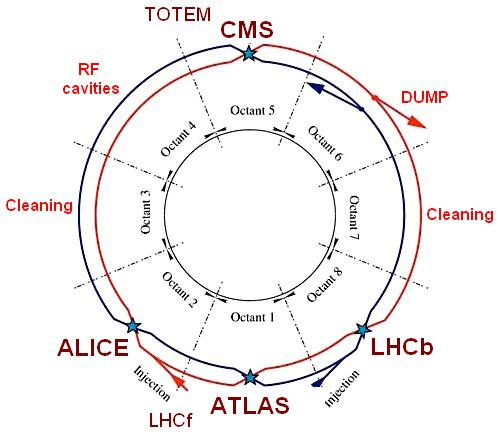
\includegraphics[width=9.6cm]{Chapter2/LHClayout.jpg}
\caption{A schematic layout of the LHC tunnel.}
\label{fig:LHClayout}
\end{center}
\end{figure}
%\vspace{-0.3in}

The eight sections are numbered from 1 to 8. The two general purpose detectors, namely,
A Toroidal LHC ApparatuS (ATLAS)~\cite{atlasTDR} and Compact Muon Solenoid (CMS)~\cite{cmsTDR} are located at point 1 and point 5 respectively. 
Point 2 is occupied by the heavy ion detector, A Large Ion Collider Experiment (ALICE)~\cite{aliceTDR} while the detector for b-physics
study, Large Hadron Collider beauty (LHCb)~\cite{lhcbTDR} is placed at point 8. These two points also have the beam injection utility for the two beams.
Collimation systems utilized for beam cleaning are placed at point 3 and 7 while the radio frequency (RF) systems for each beam are present at point 4.  
The point 6 has been used for the beam dump where the two beams are extracted vertically using horizontally and vertically deflecting magnets.
The LHC is primarily a proton-proton collider, but it also uses heavy ion beams to perform proton-lead and lead-lead collisions for some short periods of time.

\subsection{Main components of the LHC}
The design of LHC depends on very basic physics principles associated with latest technology. 
The three main components of LHC are:
\vspace{-0.1in}
\begin{enumerate}[leftmargin=*]
\item {\bf{Radio Frequency (RF) cavities}}: The RF cavities are located along the beam pipe and are used to provide acceleration to the 
  proton beams using alternating electric field. There are two independent RF systems, one for each beam. A sketch of a RF cavity is shown in the \fig{\ref{fig:RFcavity}}
  below.
  
  \begin{minipage}{0.55\textwidth}
  \begin{figure}[H]
    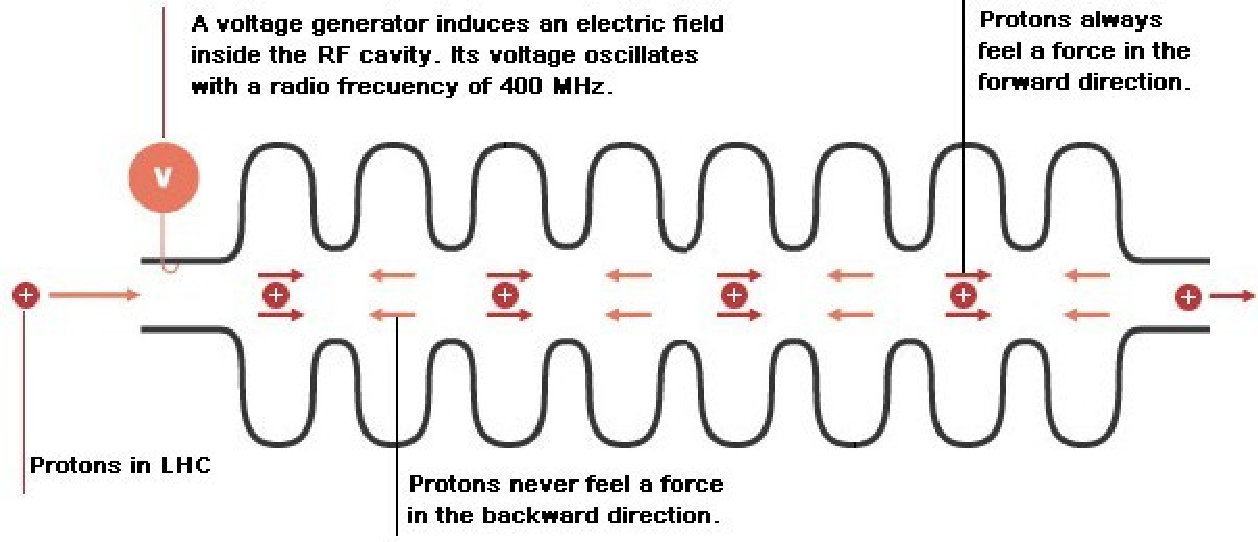
\includegraphics[width=9cm]{Chapter2/RFcavity.pdf}
    \caption{\label{fig:RFcavity} A Radio Frequency cavity.}
  \end{figure}
  \end{minipage}%
  \hfill
  \begin{minipage}{0.35\textwidth}
  \begin{figure}[H]
    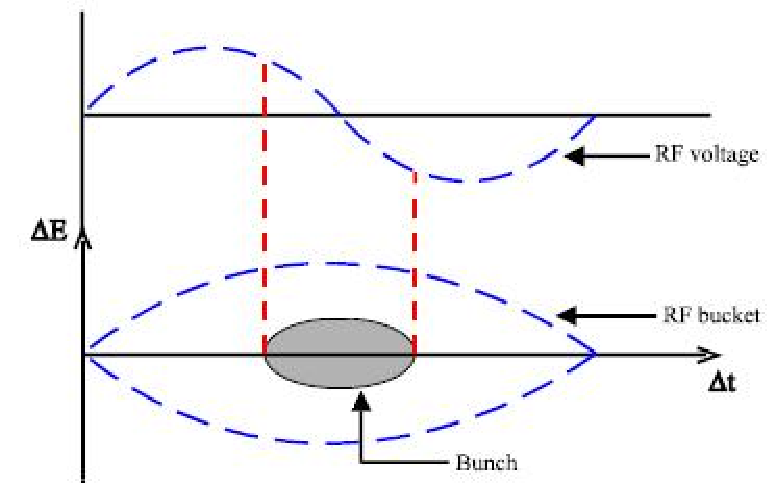
\includegraphics[width=6cm]{Chapter2/RFbucket.pdf}
    \caption{\label{fig:RFbucket} A sketch showing formation of a bunch.}
  \end{figure}
  \end{minipage}
  \vspace{0.1in}
  
  The sinusoidal varying alternating electric field of RF cavity changes polarity after each half cycle which implies that it accelerates the protons during one
  half cycle and decelerates during the other half. This results into the formation of bunches of protons. As can be seen in \fig{\ref{fig:RFbucket}}, when a proton
  arrives inside a RF cavity at a time when the voltage is zero, it will see no force and is called synchronous proton.
  Any proton arriving before the synchronous proton will see a negative polarity and hence will decelerate while any proton arriving later than
  the synchronous proton will see positive polarity and will get accelerated, so these protons will come closer to the synchronous proton and form a bunch.
  At LHC, the RF cavities resonate at a frequency of 400\unit{MHz}. The LHC is designed to have a total of 2808 bunches at a gap of 25\unit{ns}.
  The main goal of RF cavities is to maintain the tightness of proton bunches to provide high luminosity at collision points. These cavities also transfer
  the radio frequency power to the beam to provide acceleration. The LHC has eight RF cavities per beam operating at 4.5$^{^{\circ}}$\unit{K},
  each delivering a power of 2\unit{MV} at 400\unit{MHz}. 
    
\item {\bf{Vacuum chamber}}: The beam pipe in which proton beams travel are kept at a low pressure of $\sim$ $10^{-13}$ bar, much less
  than the outer space, forming an ultrahigh vacuum. This is required to minimize the interactions with parasitic particles and subsequent loss of
  accelerated protons. 
\item {\bf{Magnet system}}: In order to provide proper bending and focusing of the proton beams, an intense magnetic field varying in the range of 0.54\unit{T}
  (for 450\unit{GeV} proton energy) to 8.33\unit{T} (for 7\unit{TeV} proton energy) has been used. This high magnetic field has been achieved by the use of superconducting
  magnets made of copper plated Niobium-Titanium (NbTi) superconductors. The superconducting state has been attained by using many tones of superfluid Helium
  cooled to a temperature of 1.9$^{^{\circ}}$\unit{K}. Due to the constraints of small tunnel diameter, it was not possible to make completely
  separate rings for both the proton beams. So an alternate way was adopted in the form of twin-bore magnet design (a front view is shown in \fig{\ref{fig:LHCmagent}})
  which comprises of two coils and beam pipes
  at a separation of 180\unit{mm} within the same mechanical framework. This magnet structure is constructed in such a way that it provides
  opposite magnetic fields in the two beam pipes. The copper plated NbTi filaments are joined together to make the cables and two layers of these cables
  are wrapped around each beam pipe. The current is made to flow in opposite directions through the cables around the two pipes, which produces an intense magnetic field
  of opposite polarity in both the beam pipes. The copper provides an insulation among the NbTi filaments in superconducting state and act as a
  conductor upon reaching the conducting state.
  \begin{figure}[h]
  \begin{center}
  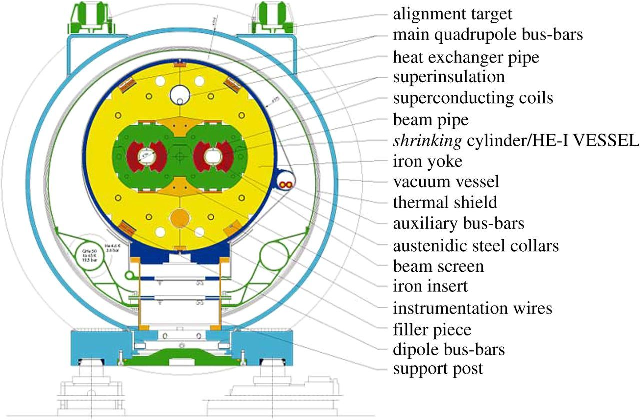
\includegraphics[width=12cm]{Chapter2/LHCmagnet.pdf}
  \caption{The LHC twin-bore magnet system}
  \label{fig:LHCmagent}
  \end{center}
  \end{figure}
%  \vspace{-0.3in}

  The LHC consists of different type of magnets that include, dipoles used for bending of the particle's beam,
  quadrupoles used for focusing of the beam, sextupoles and octupoles used for
  correcting the size and position of the beam. The LHC ring consists of 1232 dipoles, 392 quadrupoles and many sextupoles and octupoles.
  To enhance the probability of collisions, the bunches are squeezed by the use of special magnets positioned
  near the collision chambers. These magnets reduce the beam diameter to a minimum of 16 $\mu$m.

\end{enumerate}

\subsection{Proton's journey to maximum acceleration}
Making the proton beams travel closer to the speed of light is a very intricate task. At LHC, it has been accomplished
in a number of steps as can be seen in the schematic representation of CERN accelerator complex~\cite{Web:CERN} in \fig{\ref{fig:LHCring}}.
%\vspace{-0.15in}
\begin{figure}[h]
\begin{center}
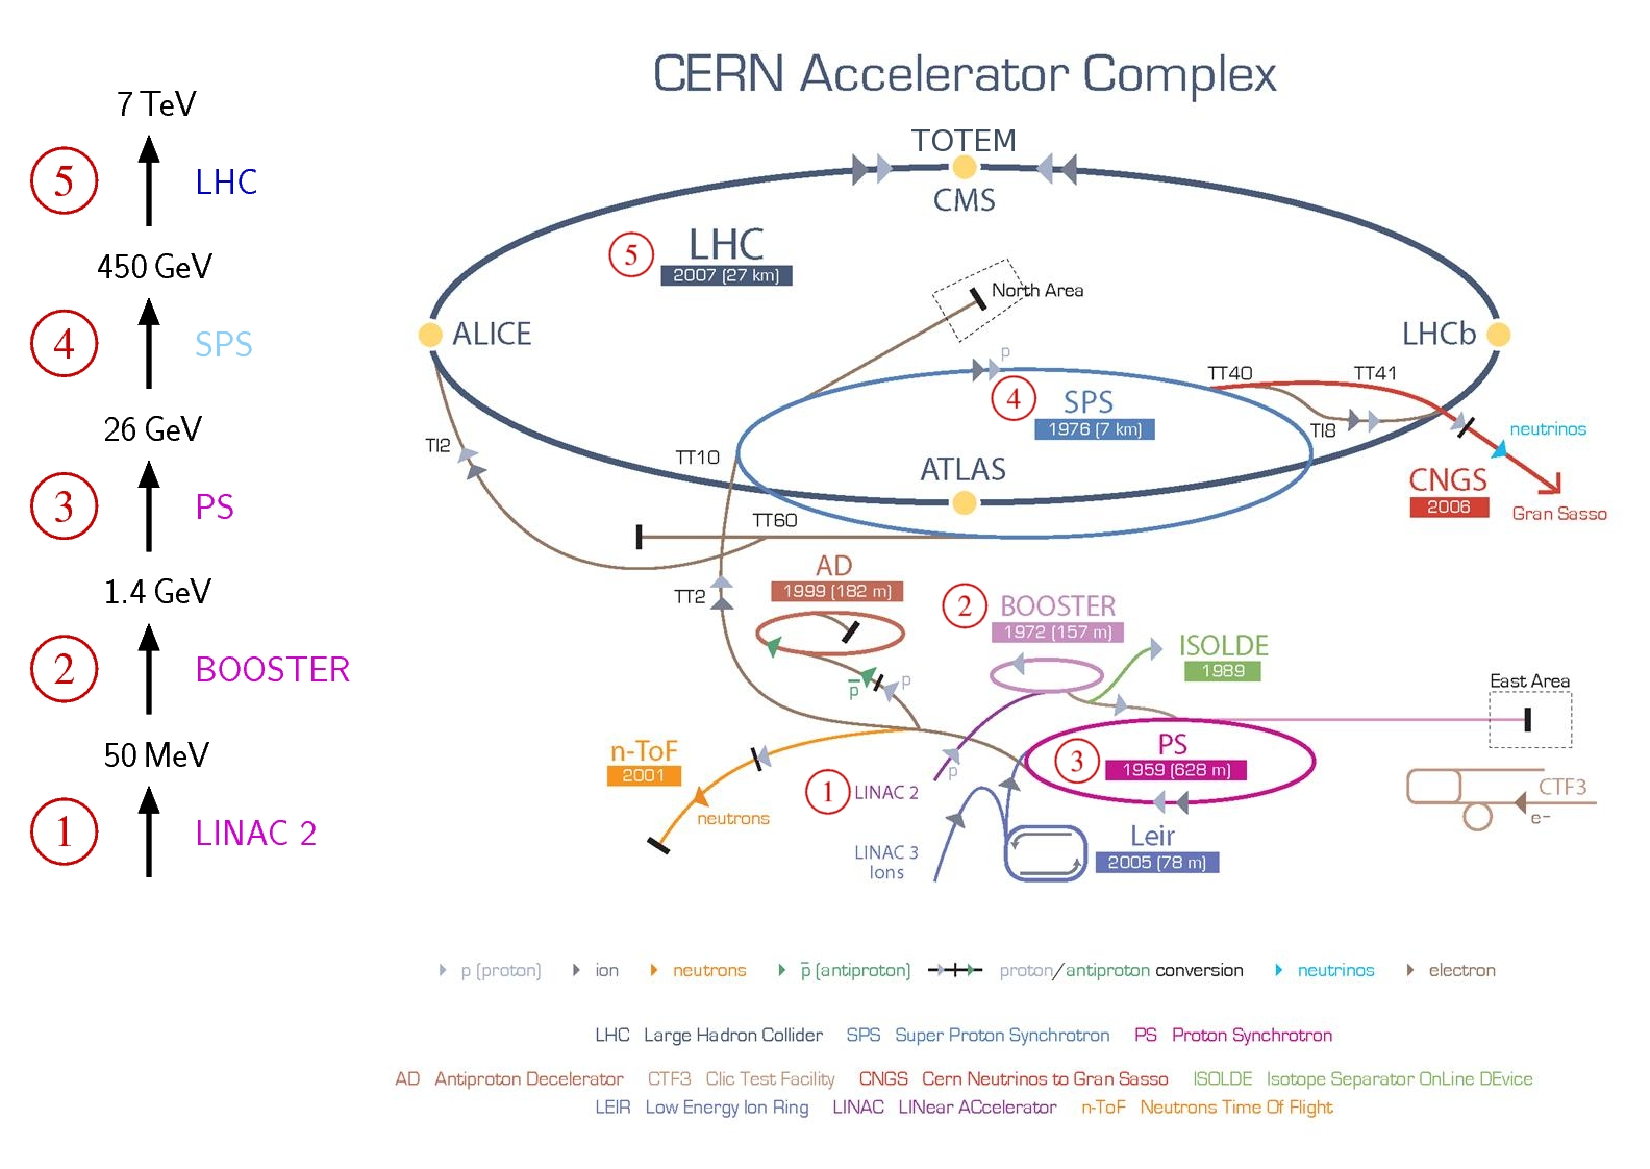
\includegraphics[width=14cm]{Chapter2/LHCRing3.pdf}
\caption{A schematic view of CERN accelerator complex representing the different accelerators deployed for providing acceleration to the proton beam.}
\label{fig:LHCring}
\end{center}
\end{figure}
%\vspace{-0.3in}
First of all, protons are extracted from hydrogen gas by stripping off the electrons using an electric discharge. Then, the protons
are directed towards a Radio Frequency Quadrupole (QRF) that provides an initial acceleration of 750\unit{keV} to the beam. After that, the protons are sent to
LINAC2, a linear accelerator that makes use of RF cavities and accelerates the proton beam upto 50\unit{MeV}. The beam from LINAC2 is made to enter
Proton Synchrotron Booster (PSB) which increases the energy of protons to 1.4\unit{GeV} and divides the proton beam into 6 bunches.
The output of PSB is then injected into Proton Synchrotron (PS) that accelerates the protons upto 25\unit{GeV}.
The PS is also responsible for preparing the LHC bunch structure. A total of 72 bunches with a spacing of 25\unit{ns} are formed in PS. The proton bunches from PS
then enter into Super Proton Synchrotron (SPS) where they are further bunched into 288 bunches and are accelerated upto the LHC injection energy of 450\unit{GeV}.
The protons from SPS are then finally made to enter into LHC where they accelerated upto the highest energy required.

\subsection{Luminosity measurements at LHC}
At LHC, the rate of collision N is expressed in terms of the instantaneous luminosity $L$ as $N$ = ${\sigma}L$ where $\sigma$ is the cross section of
the process under study. For a given process, the higher the luminosity, the
chances are more of a collision to happen. The luminosity of a beam depends upon many machine parameters and is given by,
\begin{equation}
  L = \frac{N^{2}_{b}n_{b}f_{rev}\gamma_{r}}{4\pi\beta^{\ast}\epsilon_{n}}F, 
\end{equation}
where, \\
$N_{b}$: number of particles in a bunch,\\
$n_{b}$: number of bunches in each beam,\\
$f_{rev}$: beam revolution frequency,\\
$\gamma_{r}$: relativistic gamma factor,\\
$\epsilon_{n}$: normalized transverse beam emittance\footnote{The beam emittance is defined as the transverse size of the beam. The narrower the beam, the lesser
  is the beam emittance and more are the chances of interaction.},\\
$\beta^{\ast}$: betatron function\footnote{Betatron function is defined as the distance from the
  collision point at which the beam width in transverse plane is twice compared to the beam width at collision point.}, and\\
$F$: luminosity reduction factor due to the presence of crossing angle between the two beams.
%\begin{equation}
%F = \left(1+\left(\frac{\theta_{c}\sigma_{z}}{2\sigma^{\ast}}\right)\right)
%\end{equation}

In order to achieve highly luminous beams, one need to provide large number of highly populated bunches
having low value of beam emittance and betatron function colliding at high frequencies. The various parameters related to LHC machine and proton beams
are summarized in \tab{\ref{Table:LHCParameters}}.
\begin{table}[h!]
\begin{center}
\resizebox{13cm}{!}{
%\begin{tabular}{c !{\vrule width -1pt}c !{\vrule width -1pt}c !{\vrule width -1pt}c !{\vrule width -1pt}c !{\vrule width -1pt}c !{\vrule width -1pt}c !{\vrule width -1pt}c}  %%% !{\vrule width -1pt} to make column line width less, so that white space not visible in colored table. but not working very nicely.
\renewcommand{\arraystretch}{1.2}
\begin{tabular}{lcc}
\toprule
\belowrulesepcolor{Mygray}
\belowrulesepcolor{Mygray}
\belowrulesepcolor{Mygray}
\rowcolor{Mygray}[\dimexpr\tabcolsep+0.09pt\relax]  
LHC Parameters  & Design Value & 2016 Value \\
\aboverulesepcolor{Mygray}
\aboverulesepcolor{Mygray}
\aboverulesepcolor{Mygray}
\midrule
Total number of magnets & 9600 & -- \\
Number of dipole magnets & 1232 & -- \\
Beam energy (TeV) & 14 & 13 \\
Bunch spacing (ns) & 25 & 25 \\
No. of protons per bunch & 1.1 $\times$ $10^{11}$ & 1.1 $\times$ $10^{11}$ \\
No. of bunches per beam & 2808 & 2220 \\
Beam crossing angle ($\mu$rad) & 285 & 370 \\
Beam emittance, $\epsilon_{n}$ ($\mu$m) & 3.75 & 3.4 \\
Betatron function, $\beta^{\ast}$ (m) & 0.55 & 0.4 \\
Instantaneous luminosity (cm$^{-2}$sec$^{-1}$) & 1.0 $\times$ $10^{34}$ & 1.0 $\times$ $10^{34}$ \\
\bottomrule
\end{tabular}
}
\caption{Design values of the various parameters of LHC and a comparison with the values obtained during the 2016 run.}
\label{Table:LHCParameters}
\end{center}
\end{table}
\vspace{-0.4in}


The sum of instantaneous luminosities obtained over a period of time is referred to as the integrated luminosity. The \fig{\ref{fig:LHCLumi}} shows
the total integrated luminosity delivered by the LHC and recorded by CMS~\cite{Web:CMSLumi} over a period of time for the year 2016.

\begin{figure}[h]
\begin{center}
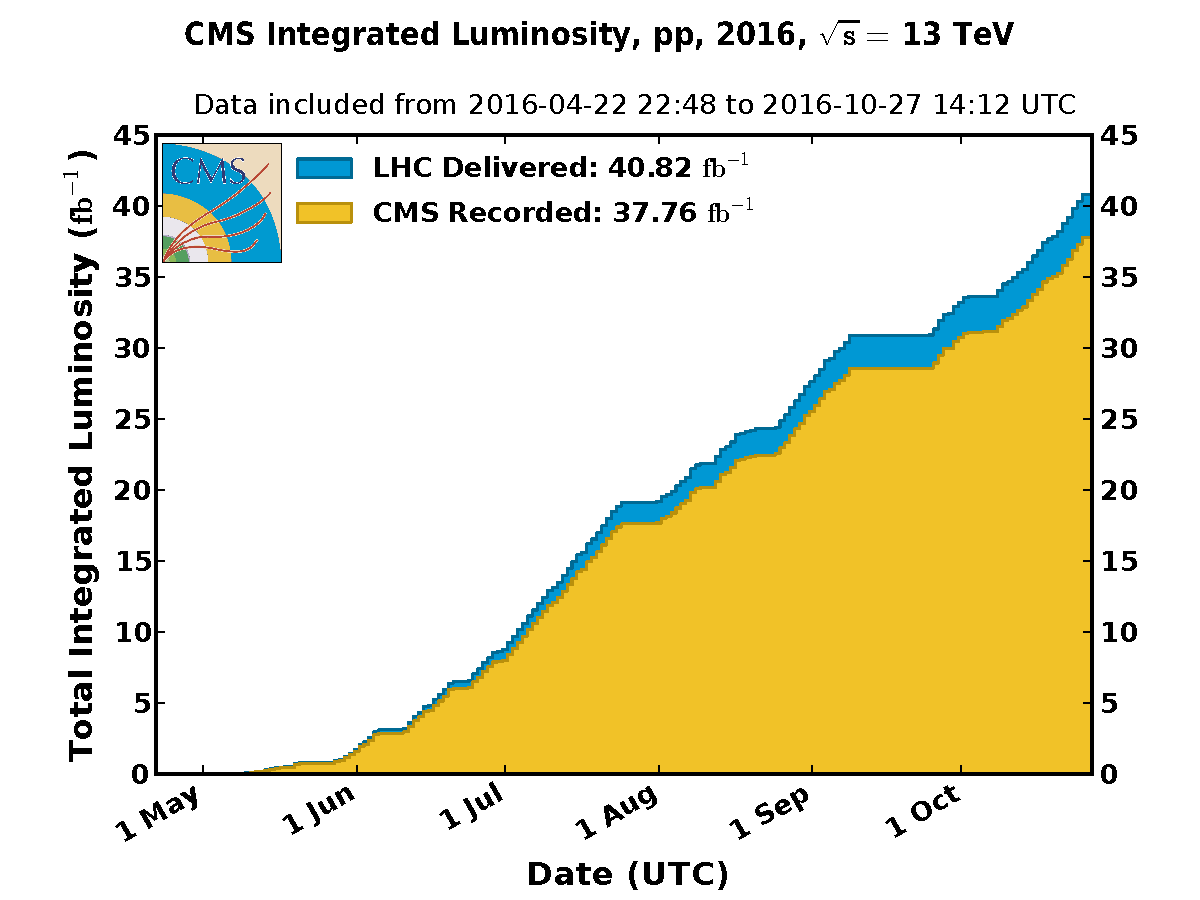
\includegraphics[width=8.6cm]{Chapter2/Int_lumi_offline_pp_2016.pdf}
\caption{Total integrated luminosity delivered by the LHC and recorded by CMS as a function of time, during the year 2016~\cite{Web:CMSLumi}.}
\label{fig:LHCLumi}
\end{center}
\end{figure}
%\vspace{-0.3in}

During the 13\unit{TeV} run in 2016, the LHC delivered a total of 40.8\fbinv of pp collision data, out of which, CMS recorded a total of 37.8\fbinv.
The CMS has certified 35.9\fbinv of recorded data to be used for physics analysis. The study presented in this thesis has been performed using this 35.9\fbinv
of data.

%%%%%%%%%%%%%%%%%%%%%%%%%%%%%%%%%%%%%%%%%%%%%%%%%%%%%%%%%%%%%%%%%%%%%%%%%%%%%%%%%%%%%%%%%%%%%%%%%%%%%%%%%%%%%%%%%%%%%%%%%%%%%%%%%%%%%%%%%%%%%%%%%%%%%%%%%%%%%%%%%%%%%%%%%%%%
%% The LHC has first started functioning in September, 2008 but halted 9 days later because of a magnet quench and helium gas explosion. It started
%% again in November, 2009 and began its first ever data taking. It recorded good physics runs for a period of around three years from March, 2010
%% to February, 2013 at a center of mass energy of 7 and 8\unit{TeV} (known as Run 1). Around $20$\fbinv\ of data collected at 8\unit{TeV} during this period
%% showed the first evidence of much awaited Higgs boson. After the Run 1, the accelerator was shut down (known as Long Shutdown 1, LS1) for next two
%% years for upgradation. It restarted again during second half of 2015 and began data taking at an increased center of mass energy of 13\unit{TeV}.
%% Its next long shut down (LS2) is scheduled to happen from 2019, it is aiming to record a data of around $100$\fbinv before that.                              
%%%%%%%%%%%%%%%%%%%%%%%%%%%%%%%%%%%%%%%%%%%%%%%%%%%%%%%%%%%%%%%%%%%%%%%%%%%%%%%%%%%%%%%%%%%%%%%%%%%%%%%%%%%%%%%%%%%%%%%%%%%%%%%%%%%%%%%%%%%%%%%%%%%%%%%%%%%%%%%%%%%%%%%%%%%%


\section{The CMS Detector}
The CMS detector~\cite{Chatrchyan:2008aa} is one of the main particle detectors designed at the LHC to observe different kind of particles and processes
produced in the pp collisions. The prime objective of the CMS detector is to explore the physics at Terascale, the energy region at which the physicists believe
the experiment has the potential to answer some of the existing key questions. The detector has a cylindrical onion like structure having a coverage of $4\pi$ steradian,
with each layer representing a different sub-detector used to measure different type of particles. The information from different layers is used to build up
the complete picture of an event. It is situated in a cavern, 100\unit{m} underground, located at point 5 of the LHC tunnel in France near village Cessy.
It has a length of 21.6\unit{m} and a diameter of 14.6\unit{m}, it weights around 14,000 tonnes.
CMS is a large scientific collaboration involving around 3,000 people from 198 scientific institutions and universities belonging to 45 countries.

\noindent
{\bf{Experimental challenges}}:\ As discussed in last section, the LHC has a very high collision rate which is achieved by colliding bunches of more than 100 billion
protons each, 40 million times every second, resulting into a pp interaction rate of around $10^{9}$ per second.
The high track density arising due to these interactions create severe radiation environment. The detector needs to remain unaffected from these radiations along with
providing efficient particle identification. The detector has to face the challenge of adjusting between occupancy and granularity.
Additionally, a majority of collisions contain uninteresting events, a fast filtering trigger system is required to reject these unwanted events.
Also, the interesting pp events are superimposed by many uninteresting events occurring in the same bunch crossing (known as pile-up).
Dealing with these events require high granularity and good time resolution detectors, which further demand to have large number of detector channels with
good synchronization. Even storing the data after huge reduction require about 10 million gigabytes per year which in itself is a big challenge.

\subsection{Layout of the CMS detector}
A general layout of the CMS detector is presented in \fig{\ref{fig:CMS_layout}}. It is based on four principle sub-systems: A high granularity central tracker,
a homogeneous electromagnetic calorimeter, a sampling hadron calorimeter and a muon detector. The heart of the CMS is its very high superconducting magnet
that is situated between the calorimeters and the muon detector. All the sub-systems of the detector are divided into one cylindrical barrel region and
two opposite facing endcap regions, complimented with very forward regions.
This arrangement provides a very good coverage of the collision fragments required for event building. A longitudinal view of the CMS detector system,
showing the barrel and endcap sections of various sub-detectors is presented in \fig{\ref{fig:CMS_longitudinal}}, with the origin denoting the interaction point.
\vspace{0.2in}

\begin{figure}[t]
\begin{center}
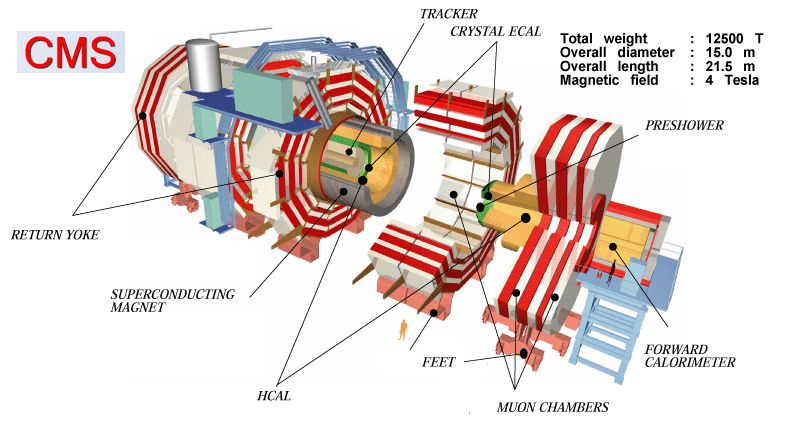
\includegraphics[width=15cm]{Chapter2/CMS_layout.png}
\caption{A layout of the CMS experiment at CERN.}
\label{fig:CMS_layout}
\end{center}
\end{figure}
%\vspace{-0.3in}


\begin{figure}[h]
\begin{center}
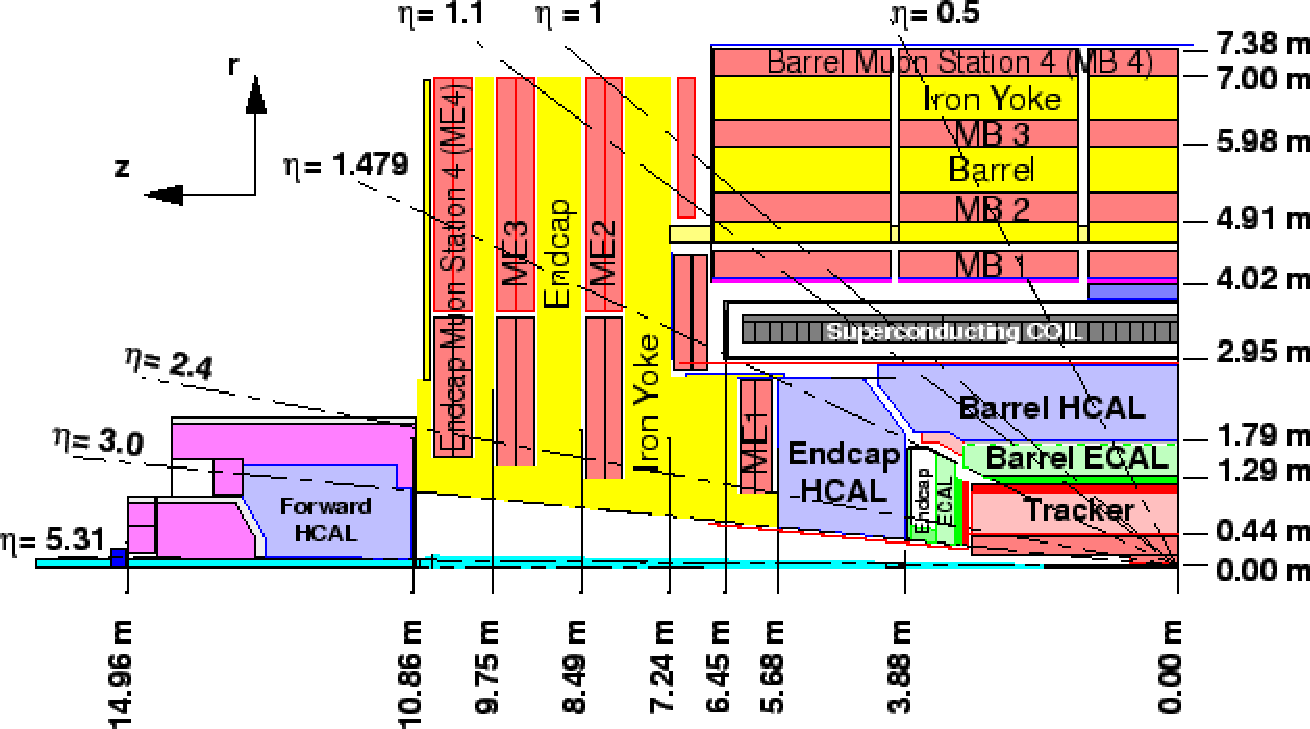
\includegraphics[width=12cm]{Chapter2/CMS_longitudinal.pdf}
\caption{Longitudinal contour of a quadrant of the CMS detector.}
\label{fig:CMS_longitudinal}
\end{center}
\end{figure}
\vspace{-0.2in}

\noindent
{\bf{Co-ordinate system}}: The CMS has adopted a right-handed spherical co-ordinate system with origin at the center of the detector which is also the
intended collision point. The $x$-axis points towards the center of the LHC tunnel, the $y$-axis is vertically upwards and the $z$-axis is along the beam pipe.
The polar angle $\theta$ is taken from the $z$-axis to the $x$-$y$ plane and the azimuthal angle $\phi$ is taken from the $x$-axis to the $y$-axis in the $x$-$y$ plane.
The angle $\theta$ denotes the particle's angle w.r.t the beam axis while angle $\phi$ denotes the particle's orientation in the transverse plane.
The co-ordinate $r$ denotes the radial distance and is defined by $r$ = $\sqrt{x^{2}+y^{2}+z^{2}}$.
It is conventional to use pseudorapidity $\eta$ instead of polar angle $\theta$ as 
seen in \fig{\ref{fig:CMS_longitudinal}}. The pseudorapidity is defined in terms of angle $\theta$ as
\begin{equation}
  \eta = -\ln\left[\tan\frac{\theta}{2}\right].
\end{equation}
On going from -$z$ to +$z$ axis, $\theta$ goes from -$\pi$ to +$\pi$ and $\eta$ goes from -$\infty$ to +$\infty$. In the non-relativistic limit,
it is called rapidity and is defined as,
\begin{equation}
  y = \frac{1}{2}\ln\left(\frac{E + p_{z}}{E - p_{z}}\right),
\end{equation}
where $E$ and $p_{z}$ are the particle's energy and $z$-component of the momentum. The rapidity, $y$ requires the measurement
of both $E$ and $p_{z}$ and in relativistic regime, it is quite difficult to measure the $z$-component of momentum very precisely.
The reason of choosing $\eta$ over $\theta$ is that the difference between
the pseudorapidity of two particles ($\Delta\eta$) is Lorentz invariant under boosts along the beam axis. This means that an observer in the lab frame, boosted
along $z$-axis w.r.t the rest frame, will measure the same $\Delta\eta$ between two particles as an observer in the rest frame.
The importance of this feature comes from the fact that in the pp collisions, the hard interaction takes place between proton constituents (quarks or gluons),
usually having different momenta, which means the different interactions have different boosts of their center-of-mass frames w.r.t the detector rest frame.
Invariance of $\Delta\eta$ under boosts allows us to treat the different interactions in a similar way as the interaction happening in the center-of-mass rest frame.
The various histograms binned on the angular separation of particles will remain undistorted by these arbitrary boosts of different events.
The angular distance $R$ between two particles in $\eta-\phi$ plane, as observed from the origin of CMS detector,
is written in terms of the differences in $\eta$ and $\phi$ as, $R$ = $\sqrt{({\Delta\eta})^{2}+({\Delta\phi})^{2}}$.

In colliders, two particle beams colliding head-on consist of only longitudinal component of momentum. So the particles in the beam do not have a transverse component
of momentum before collision, thus by conservation of momentum, the total transverse momentum after the collision should also add up to zero. This feature is
extensively used in collider experiments and it requires to consider the
particle's energy and momentum in the transverse direction, known as transverse energy (\et) and transverse momentum (\pt), defined as
\et = $E\sin\theta$ and \pt = $\sqrt{p_{x}^{2} + p_{y}^{2}}$ respectively.  
Any imbalance in the transverse momentum is caused by either the invisible particles like neutrinos or by the energy lost in the unavoidable nuclear processes.
This imbalance is known as missing transverse energy and is given by, \met = -$\sum{\pt}$.
    
A short description of all the components of the CMS detector from innermost to outermost has been provided as follows:

\subsubsection{CMS tracking system}\label{Se:CMS_tracker}
The tracker~\cite{Chatrchyan:2008aa,Karimaki:368412} is the innermost sub-detector, installed close to the interaction point. It has been designed to
build tracks of charged particles coming out of the collisions and reconstruct primary as well as secondary vertices, with utmost precision and accuracy.     

The tracker has a total length of 5.8\unit{m}, a diameter of 2.5\unit{m} and covers a region upto $|\eta|$ $<$ 2.5.
A uniform magnetic field of 3.8\unit{T} is present over its entire volume. 
A cross-sectional view of the CMS tracker has been presented in \fig{\ref{fig:CMS_tracker}}. The tracker is made up of a central barrel and
endcap parts consisting of pixel and strip layers. Both pixel and strip layers are made up of silicon sensors of different dimensions.
The CMS tracker is the world's largest silicon tracker with over 200$\unit{m}^{2}$ of active silicon area. 
Whenever a charged particle passes through a silicon sensor, it results into generation of electron-hole pairs,
which are measured in an outer circuit as a hit. Subsequent information of the large number of hits from different sensors
leads to the reconstruction of the particle's track.
Since the energy required to generate an electron-hole pair is small, the energy$/$momentum resolution of these sensors
is very large. Also, since the electrons travel very fast to the outer circuit, the time resolution is better. 
The charged particles of different momentum curved differently under the effect of
the magnetic field and the tracker records the particle's tracks and momentum by finding their positions and curvature at various key points.  

\begin{figure}[h]
\begin{center}
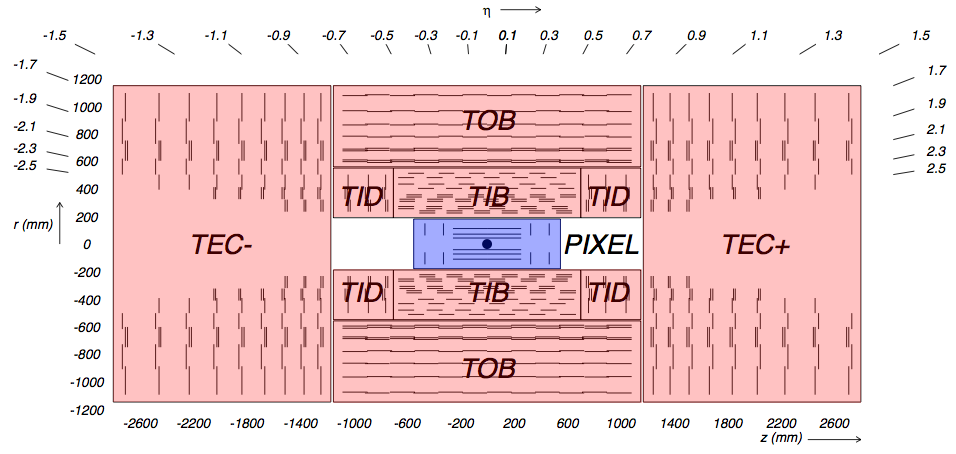
\includegraphics[width=13.4cm]{Chapter2/CMS_tracker.png}
\caption{A cross-sectional view of the CMS tracker system in $r$-$z$ plane, with each line representing a silicon detector module.}
\label{fig:CMS_tracker}
\end{center}
\end{figure}
\vspace{-0.3in}

The tracker has to face around 1000 particles coming from each bunch crossing at every 25\unit{ns} which lead to high radiation doses in the detector. So it should
be able to operate in such a harsh environment in addition to dealing with high occupancy rate as well as providing high granularity and
quick response~\cite{Chatrchyan:2014fea}. The silicon detector technology meets all these goals very efficiently. 
The number of tracker layers is a tradeoff among the tracking efficiency and material budget~\cite{CMS:2010nua}.
On one side, more layers leads to more hits and precise track reconstruction. While on other side, large amount of
material inside the tracker leads to multiple scattering which in turn can spoil proper tracking too.

In order to reconstruct a track using hits, the simplest approach is to start from a hit in the innermost layer and in radial direction, project a cone on the next layer.
If the next layer contains no hit within the cone, leave the starting point considering it a noise or a particle of very low energy. Otherwise, keep on repeating the
procedure until last layer is reached. A more advanced approach start the search from the outermost layer along with taking additional information from other sub-detectors.
A description of pixel and strip layers of CMS tracker has been provided below.

\paragraph {\bf{Pixel detector}}
\hspace{\parindent} The high precision pixel detector~\cite{Baur:1999tw} is the innermost detector of the CMS tracker. Since the particle flux near
the collision point is very large, a small-scale pixel geometry is constructed to achieve unambiguous track reconstruction and precise vertex determination.
The particles with relatively long lifetime, such as b and c quarks, arise from primary vertex but decay after travelling small distances, forming secondary
vertices. The pixel detector is designed to distinguish these secondary vertices from the primary collision point.

The pixel detector consists of three concentric barrel layers and two endcap disks on both sides (shown in \fig{\ref{fig:CMS_PixelDet}}),
covering a pseudorapidity region of $|\eta|$ $<$ 2.5. The barrel layers are 
53\unit{cm} long and are present at the radii of 4.4, 7.3 and 10.2\unit{cm} from the beam line. The two endcap disks are extended in radius from 6\unit{cm} to 15\unit{cm}
and are present at $\pm$34.5 and $\pm$46.5\unit{cm} from the collision point. The detector is equipped with a total of about 66 million pixels, each
having a size of 100$\times$150${\mu{m}}^{2}$.
The occupancy rate of each pixel is of the order of 0.1$\%$ per LHC bunch crossing.  

\begin{figure}[h]
\begin{center}
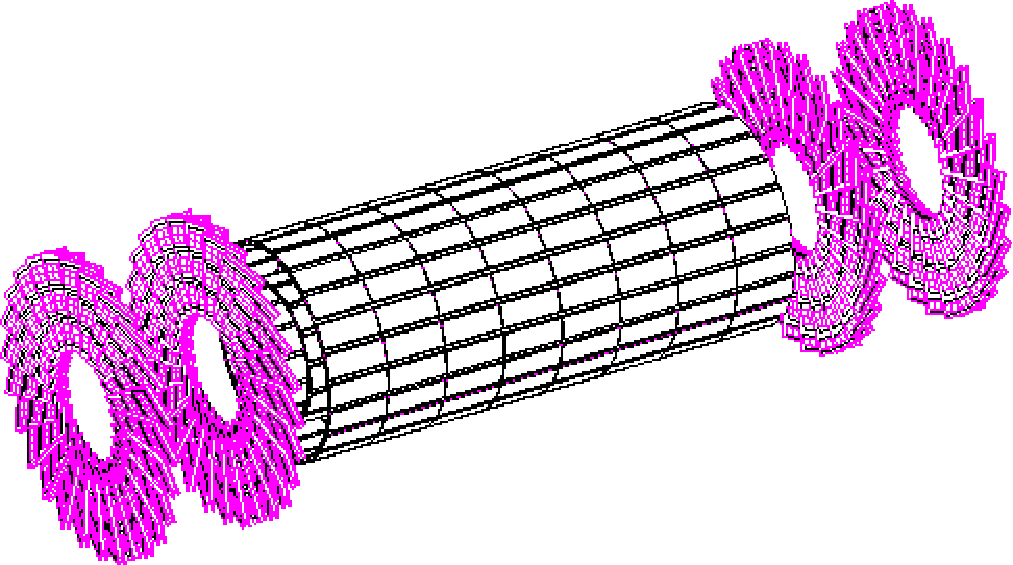
\includegraphics[width=8cm]{Chapter2/CMS_PixelDet.pdf}
\caption{A schematic layout of the CMS pixel detector.}
\label{fig:CMS_PixelDet}
\end{center}
\end{figure}

The pixel detector has performed exceedingly well during Run I, providing a resolution of
around 10{$\mu${m}} in $r-\phi$ and 20-40{$\mu${m}} in $z$
direction along with an overall efficiency of more than 99$\%$. The LHC Run II started in 2015 with an increased center of mass energy of 13\unit{TeV}
and a lower bunch crossing frequency of 25\unit{ns}. During overall Run II phase,
a peak instantaneous luminosity of 2 $\times$ $10^{-34}\unit{{cm}^{-2}{s}^{-1}}$ was achieved.
It also saw a pileup rate of more than 50. Under these conditions, the current pixel detector will suffer from increased fake rates and reduced resolution
due to higher occupancy. So in order to maintain the performance of pixel detector, an upgrade known as
``Phase1 Pixel Upgrade''~\cite{CMS:2012sda,1748-0221-9-03-C03041} was
performed during the technical stop at the end of 2016. The upgraded pixel detector features 4 barrel layers and a turbine-like module arrangement for endcap
disks (as shown in \fig{\ref{fig:Pixel_upgrade}}). Light-weight support structures and 2-phase CO$_{2}$ cooling has been introduced to keep the optimum material budget.  
A comparison of the two detector configurations using tracking efficiency and fake rate as a function of pileup are presented in \fig{\ref{fig:Pixel_upgrade_effects}}.

\begin{figure}[h]
\begin{center}
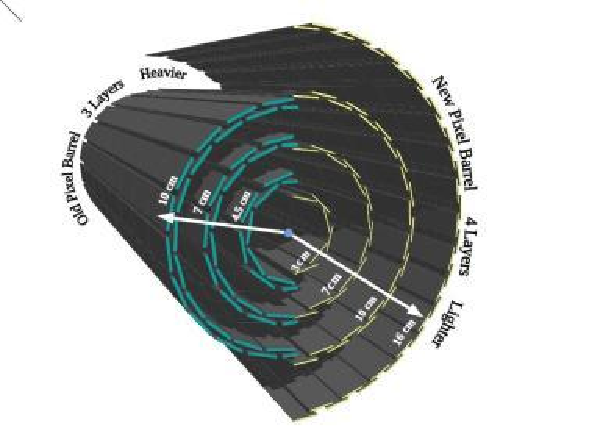
\includegraphics[width=7cm]{Chapter2/PixelDetector_barrel_oldvsNew.pdf}
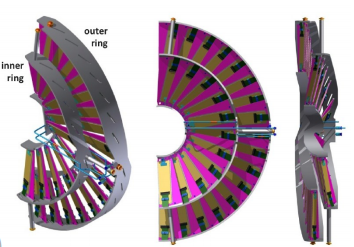
\includegraphics[width=7.5cm]{Chapter2/Pixel_upgrade_endcaps.png}
\caption{A schematic representation of the upgrades in pixel detector barrel (left) and endcaps (right) during Phase1 Pixel Upgrade.}
\label{fig:Pixel_upgrade}
\end{center}
\end{figure}
\vspace{-0.3in}

\begin{figure}[h]
\begin{center}
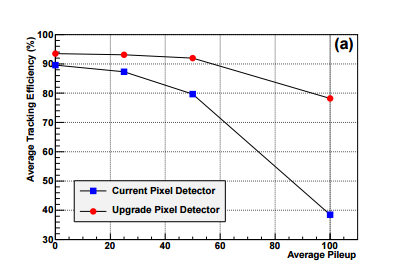
\includegraphics[width=7.2cm]{Chapter2/PixelUpgrade_trackEff.png}
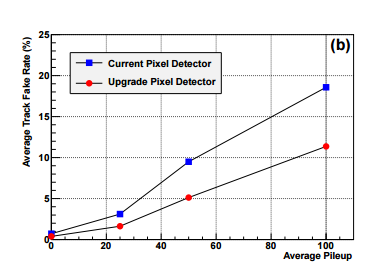
\includegraphics[width=7.2cm]{Chapter2/PixelUpgrade_fakerate.png}
\caption{Performance measurement of the older pixel detector (blue) and the upgrade pixel detector (red) using $\textrm{t}\bar{\textrm{t}}$ events,
  showing tracking efficiency (left) and fake rate (right) as a function of per event pileup~\cite{1748-0221-9-03-C03041}.}
\label{fig:Pixel_upgrade_effects}
\end{center}
\end{figure}

\paragraph {\bf{Silicon strip detector}}
\hspace{\parindent} The silicon strip tracker~\cite{Chatrchyan:2008aa,Karimaki:368412} is present outside the pixel detector
  and consists of more than 15000 single or double sided (shown in \fig{\ref{fig:CMS_tracker}} by single and double lines)
  modules. Since the particle flux reduces in strip tracker,
  the dimensions of strip modules are kept larger than that of pixel detector modules. The size of modules also increases with distance to keep the occupancy level
  at around 1$\%$. The modules are of rectangular shape in barrel region while that of trapezoidal shape in the endcap region.
  The strip tracker consists of four subsystems: The Tracker Inner Barrels (TIB), Tracker Inner Disks (TID), Tracker Outer Barrels (TOB) and
  Tracker EndCaps (TEC).

  The TIB and TID are extended up to a radius of 55\unit{cm} and consists of 4 barrel $+$ 3 endcap layers. The modules in TIB$/$TID are 320{$\mu${m}} thick and
  delivers up to 4 measurements in $r-\phi$ direction, providing a position resolution of 23{$\mu${m}} in the inner two layers and 35{$\mu${m}} in the outer two layers.
  The outer barrel layer TOB is made up of 6 layers of 500{$\mu${m}} thick sensors extended up to an outer radius of 116\unit{cm} which provides 6 more measurements
  in $r-\phi$ direction, corresponding to a resolution of 53{$\mu${m}} in the initial four layers and 35{$\mu${m}} in the last two layers.
  The TOB covers a $z$ range up to $\pm$118\unit{cm}.
  Outside this range, $\pm$TEC occupies the region from $124-282$\unit{cm} in ${\pm}z$ and $22.5-113.5$\unit{cm} in ${\pm}r$. Each of the TEC is made up of 9 disks, thereby
  providing 9 measurements in $r-\phi$ per trajectory. 

  The transverse momentum resolution of the tracker varies in the range from 0.7$\%$ at 1\unit{GeV} to 1.5$\%$ at 100\unit{GeV}.

\subsubsection{Calorimeter}
A calorimeter is a device that is used to measure energies of different type of particles. The incident particle interacts with the material of the calorimeter and
produces a cascade (shower) of secondary particles of progressively lower energies, until the energies fall below a critical value which is then
dissipated in ionization or excitation of the atoms of the material. The subsequent energy released by the atoms is captured by the photo-detector which through
photoelectric effect, yield an electronic signal that provides a measurement of the particle's energy.
In case of the sampling calorimeters, the medium that activate the particle shower is known as the passive medium (absorber)
while the one that absorb the shower particles and lead to the energy measurement, is known as the active medium (scintillator).
Calorimeters has the capability to stop almost all particles except muons and neutrinos. 

Calorimeters are broadly divided into two categories: Hadronic and Electromagnetic, depending on the particle type. They can also be classified
on the basis of their composition into sampling and homogeneous calorimeters. A sampling calorimeter is the one that consists of alternate layers of
two materials acting as passive and active mediums while a homogeneous calorimeter is build up of only one type of material that accomplish both the tasks.
An advantage of sampling configuration is that both the materials used are well-suited for their tasks. A very high density material is used as passive medium
which results into the quick evolution of the shower into a limited space, so sampling calorimeters can be made compact as compared to homogeneous calorimeters.
However, it has a disadvantage that part of the shower energy get deposited in the passive medium and left unmeasured. 

The CMS consists of Electromagnetic calorimeter (ECAL) just outside the tracker, followed by Hadronic calorimeter (HCAL), both contained inside the solenoidal magnet.
A short description of each one is considered below.

\paragraph{Electromagnetic calorimeter}
\hspace{\parindent}
The CMS ECAL measures the energy of electromagnetically interacting particles, primarily photons and electrons. The photons interact with the material of the detector
mainly through pair production for energies above 1\unit{MeV} and through Compton scattering and photoelectric effect for energies below 1\unit{MeV}.
On the other hand, electrons mainly interact via bremsstrahlung for energies above 10\unit{MeV} and through ionization and excitation for energies below it.
As a consequence, high energy electrons and photons, inside ECAL, produce a number of secondary particles, thereby generating electromagnetic (EM) showers.
The EM showers are characterized by a material dependent parameter, the radiation length denoted as $X_{0}$, which is the average distance $x$ travelled by an electron
before losing an energy equivalent to $1/e$ times its original energy \ie $E = E_{0}e^{-\frac{x}{X_{0}}}$.
It is also equivalent to $7/9$ times the free path travelled by photon before converting into an $e^{+}e^{-}$ pair.

As a result of particle multiplication and faster interaction, the amount of material required to contain an EM shower is rather small. Therefore,
the ECAL~\cite{Chatrchyan:2008aa, ecalTDR} (shown in \fig{\ref{fig:ECAL}})
is constructed as a homogeneous calorimeter made up of lead tungstate (PbWO$_{4}$) scintillating crystals.
It is a highly dense material (8.28$\unit{g/{cm}^{3}}$) with a radiation length of 0.89\unit{cm} and Moli$\grave{\textrm{e}}$re radius of 2.2\unit{cm},
allowing a design of fast, granular and radiation resistant calorimeter.
The crystals are designed to provide very good energy resolution of electrons and photons required for CMS physics program. 
These are arranged in carbon fibre matrices to provide optical isolation.  


\begin{figure}[h]
\begin{center}
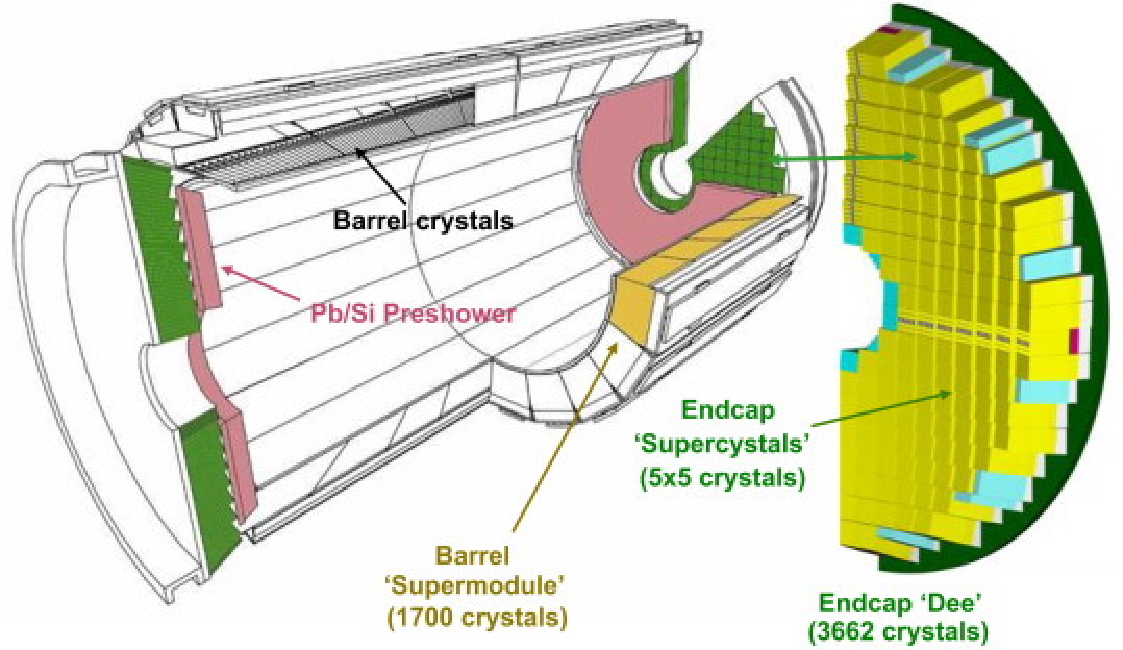
\includegraphics[width=11cm]{Chapter2/ECAL_layout.pdf}
%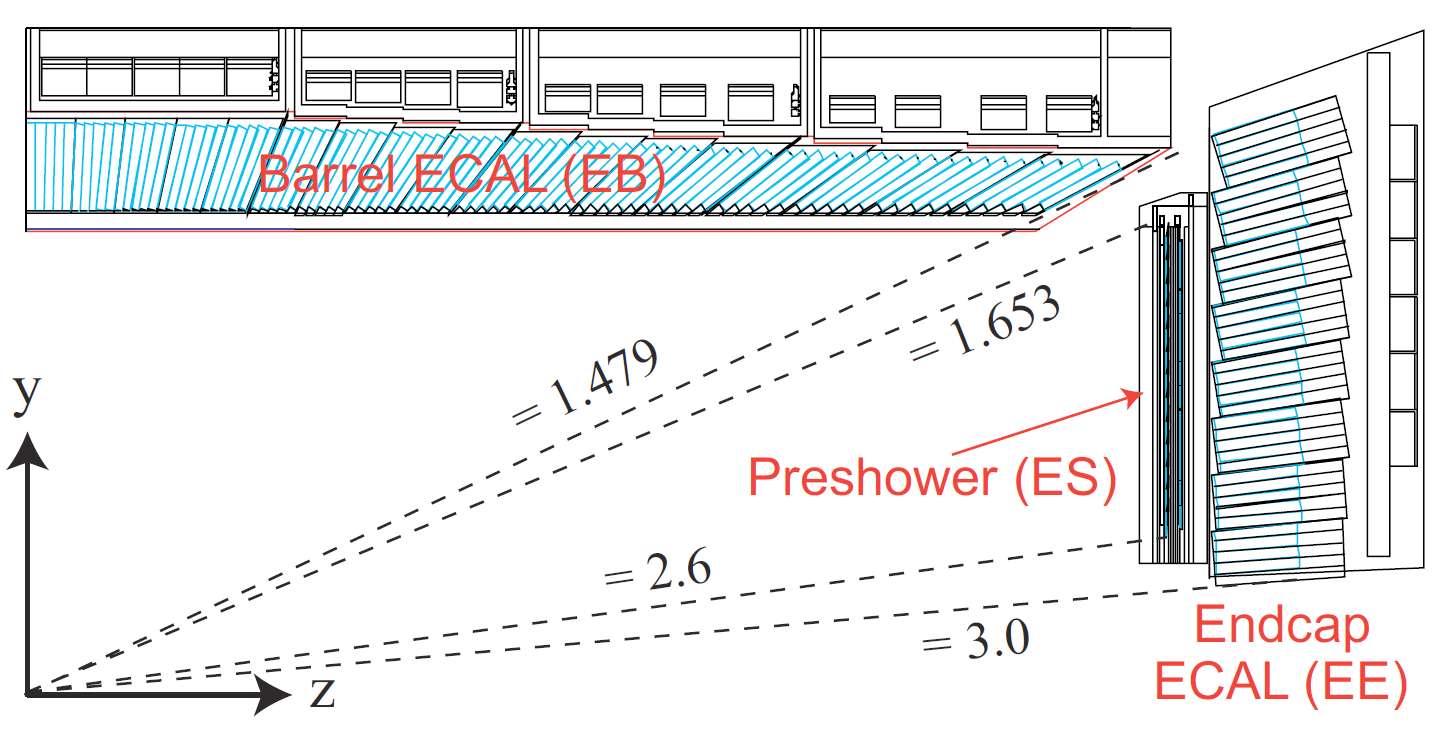
\includegraphics[width=6.5cm]{Chapter2/ECAL_positioning.png}
\caption{A layout of the CMS Electromagnetic calorimeter displaying the arrangement of crystals in barrel and endcaps with the preshower present in front.}
\label{fig:ECAL}
\end{center}
\end{figure}
\vspace{-0.3in}

The ECAL barrel (EB) is extended upto $|\eta|$ $<$ 1.479 and consists of 61,200 crystals providing 360-fold granularity in $\phi$ and (2$\times$85)-fold
granularity in $\eta$ direction. The crystals are of trapezoidal shape having a front cross section of 22$\times$22$\unit{mm}^{2}$,
a rear cross section of 26$\times$26$\unit{mm}^{2}$ and
a length of 230\unit{mm}, equivalent to 25.8$X_{0}$ implying that it is able to contain 99.999$\cdots\%$ of $e/\gamma$ energy. These crystals are assembled
into 36 supermodules, each weighing around 3 tonnes and containing 1700 crystals. Each supermodule covers 20$^{^{\circ}}$ in $\phi$ and half barrel in $\eta$.
The avalanche photodiodes (APDs) are used as photo-detectors to capture the scintillating light generated in the crystals upon interaction. These are made up of
semiconducting silicon and have an active area of 5$\times$5$\unit{mm}^{2}$. The relatively low light yield of PbWO$_{4}$ crystals is compensated by the
signal amplification by APDs through avalanche process. In addition, insensitivity of APDs towards high magnetic field and high radiation environment, makes them
convenient for EB. 

The flat circular ECAL endcaps (EE) cover the barrel at both the ends in the pseudorapidity range 1.479 $<$ $|\eta|$ $<$ 3.0, each consisting of 7,324 crystals arranged
in 5$\times$5 crystal units, known as supercrystals. The trapezoidal crystals have a front face of
28.62$\times$28.62$\unit{mm}^{2}$, a rear face of 30$\times$30$\unit{mm}^{2}$
and a length of 220\unit{mm} (24.7$X_{0}$). Endcaps use vacuum phototriodes (VPTs) as photo-detectors since these can work in high radiation environment compared to
APDs. Each VPT has a diameter of 25\unit{mm} and an active area of 280$\unit{mm}^{2}$. In front of each ECAL endcap is present a high granularity sampling calorimeter,
known as ECAL Preshower (ES), made up of alternating layers of lead (passive medium) and silicon strips (active medium). It covers a pseudorapidity range of
1.653 $<$ $|\eta|$ $<$ 2.6 and forms a disc of 2.5\unit{m} circumference. The disc is about 20\unit{cm} thick and has a 50\unit{cm} diameter hole in the middle
for the passage of beam pipe. The principle aim of ES is to identify and stop overlapping photons coming from the decay of $\pi^{0}$ so as to prevent
false signals. The high density of lead stimulate quick showering, thereby resulting into the shower containment in
a very small volume. Around 95$\%$ of incident photons start showering in the first lead plane. 

Many contributions deteriorate the actual energy resolution of any realistic calorimeter. The energy resolution of ECAL
(for energies below 500\unit{GeV}) can be written in general as:
\begin{equation}
  \frac{\sigma}{E} = \frac{S}{\sqrt{E}} \oplus \frac{N}{E} \oplus C
\end{equation}
where $\oplus$ corresponds to quadratic sum which implies that the contributions of different terms are independent from each other. The first term $S$
is known as stochastic or sampling term. It considers the statistical fluctuations due to the shower fluctuations, lateral shower leakage,
photo-detector inefficiencies, efficiency loss due to the shower containment in the passive medium of preshower etc. The second term $N$ corresponds to the
noise term arising due to instrumental effects, light-attenuation, pileup effects etc. The last term $C$ is a constant term and it includes effects from
imperfections in calorimeter construction, inter-calibration errors, longitudinal shower leakage, fluctuation in energy deposition in the dead areas of calorimeter etc.


The test beam studies~\cite{Chatrchyan:2013dga} were performed using a block of 3$\times$3 crystals and various terms involved in energy resolution were computed. These terms
for barrel region are: $S$ = 2.8$\%$, $N$ = 124\unit{MeV} and $C$ = 0.3$\%$ while for endcap region are: $S$ = 5$\%$, $N$ = 500\unit{MeV} and $C$ = 0.3$\%$.

\paragraph{Hadronic calorimeter}
\hspace{\parindent} The CMS HCAL has been designed to measure energy of particles (hadrons) interacting via strong force. Hadrons interact with the material
of the detector through strong nuclear interactions, resulting into the production of a large number of
secondary hadrons, thereby activating a hadronic shower. A majority of these shower particles, around 90$\%$, are pions. Among these, the neutral pions ($\pi^{0}$)
decay electromagnetically into two photons, thereby generating a component of EM shower within a hadronic shower. The fraction of energy of a hadron taken off
by the EM component is denoted as $f_{\textrm{EM}}$ and it varies from event-to-event. This fraction depends on the energy of initial hadron and
varies from 30$\%$ for a 10\unit{GeV} hadron to 50$\%$ for a 100\unit{GeV} hadron. Also, a significant fraction of
shower particles lose their energy as nuclear binding energy in nuclear reactions. This energy does not appear as a signal in the calorimeter and therefore, dissipate as
invisible energy. As a consequence, the calorimeter signal for a hadron is usually smaller than an electron having same energy,
a phenomenon known as non-compensation, also denoted as $e/h$ ratio. These two features of hadron showers result into a non-linearity in
the energy measurement of hadrons by HCAL.

The shower profiles of hadrons are characterized by nuclear interaction length, $\lambda_{\textrm{int}}$ (expressed in $\unit{g/{cm}^{2}}$)
which is the mean distance traversed by a hadron before undergoing a nuclear interaction. Usually, the interaction length of a hadron is much larger than
the radiation length of an electron of same energy, e.g. in copper, $X_{0}$ = 1.4\unit{cm} while $\lambda_{\textrm{int}}$ = 15\unit{cm}. 
This implies that a large amount of material is required to contain a hadron of a particular energy compared to an electron of same energy, not
possible to achieve with homogeneous calorimeter. Therefore, the hadron calorimeter always use sampling configuration. A properly designed sampling detector achieves
compensation of hadronic signals by the use of various techniques and sampling fractions~\cite{Wigmans:1991cc}.

The HCAL~\cite{hcalTDR} is a sampling calorimeter constructed of a dense absorber material made up of brass$/$steel plates interleaved with plastic scintillator tiles,
which are read out via embedded wavelength-shifting (WLS) fibres. This configuration is chosen for both barrel and endcap regions of HCAL
due to the non-magnetic behaviour, high absorption length and
good mechanical strength of brass while long term stability and radiation hardness of plastic scintillators. The detector is assembled in such a way that it
does not have any cracks or dead areas in $\phi$. The scintillator
tiles emit blue-violet light upon particle interaction, which is then converted into green light by WLS fibres. These optical signals are then converted into
electronic signals by the use of Hybrid Photodiodes (HPDs).
The HCAL constitutes of four sections: HCAL Barrel (HB)~\cite{Abdullin:2008zzb},
HCAL Endcaps (HE)~\cite{Baiatian:2008zz}, HCAL Forward (HF)~\cite{Bayatian:2006jz}, and HCAL Outer (HO)~\cite{Abdullin:2008zza}. The HCAL, in association
with ECAL, provides the energy$/$direction measurements of hadrons. A schematic view of a section
of HCAL is presented in \fig{\ref{fig:HCAL}}.

\begin{figure}[h]
\begin{center}
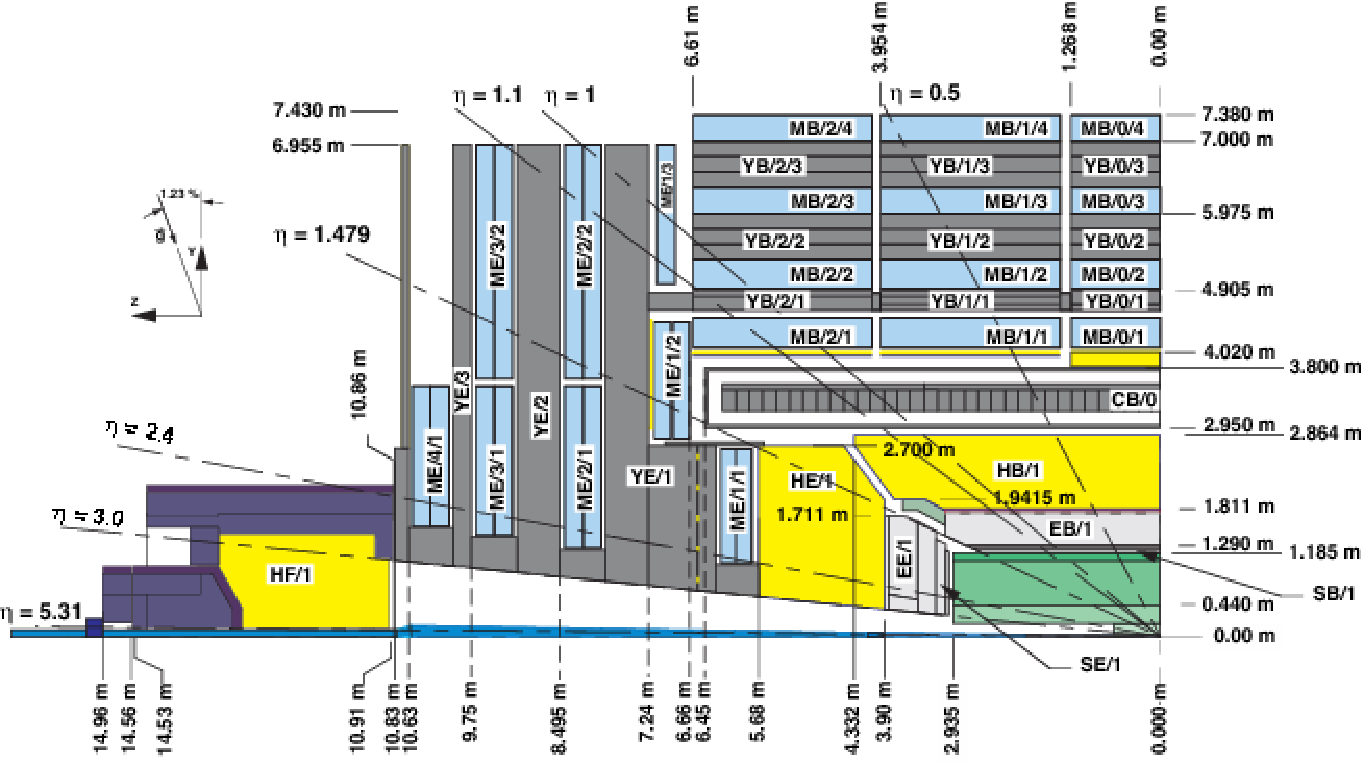
\includegraphics[width=13cm]{Chapter2/HCAL_layout.pdf}
\caption{A schematic view of a quadrant of the CMS Hadron calorimeter presenting different sub-detectors (in yellow color).}
\label{fig:HCAL}
\end{center}
\end{figure}
\vspace{-0.3in}

The HCAL barrel covers a pseudorapidity range of $|\eta|$ $<$ 1.3 and is made up of two half barrels, each made of 18 azimuthal wedges,
each covering 20$^{^{\circ}}$ in $\phi$. Each wedge is sliced into 16 absorber plates, with front and back plates made of
steel and rest made of brass (a Cu-Zn alloy). The plastic scintillating tiles with WLS fibres are arranged into trays containing many tiles and
are inserted between each plate to construct a sampling configuration. Each wedge is further partitioned into 4$\phi$ sectors while
the plastic scintillators are further partitioned into 16$\eta$ sectors, resulting into a segmentation of $\Delta\phi$ $\times$ $\Delta\eta$ = 0.087 $\times$ 0.087.
The HB is situated between EB (at $r$ = 1.77\unit{m}) and superconducting magnet (at $r$ = 2.95\unit{m}), resulting into highly constrained material amount.
The total thickness of HB corresponds to 5.82$\lambda_{\textrm{int}}$ at $\eta$ = 0 and 10.6$\lambda_{\textrm{int}}$ at $\eta$ = 1.3, ECAL also adds a thickness of
1.1$\lambda_{\textrm{int}}$ to HB material. In order to ensure the proper energy containment of hadronic showers, a complementary detector layer of same
configuration known as HO, is positioned outside the magnet coil which acts as a tail-catcher for any late starting showers.
It provides an additional thickness of 1-2$\lambda_{\textrm{int}}$ to HB showers. The high pseudorapidity region, 1.3 $<$ $|\eta|$ $<$ 3.0 has been
instrumented using HE on both sides of HB. The endcaps are made of 17 brass plate layers with plastic scintillator tiles accommodated in between. Including with EE,
it corresponds to a total thickness of around 10$\lambda_{\textrm{int}}$.

The high radiation environment (3.0 $<$ $|\eta|$ $<$ 5.0) near the beam pipe is armed with a more robust hadron forward (HF) calorimeter made up of quartz fibres
as active medium and steel as the absorber medium. The front face of HF is located at a distance of 11.2\unit{m} from the interaction point. The structure is
divided into 36 azimuthal wedges of steel, 18 wedges on each side of collision point and composed of 5\unit{mm} thick scintillator plates along with WLS fibres.     
A signal in the form of Cherenkov radiation is produced in HF when a charged particle from the shower enters the active medium (quartz)
with a velocity greater than that of light in the medium. The HF has been utilized
to improve the $\met$ measurements and identify$/$reconstruct very forward jets which can contain distinguishing features of many physics processes.
The HF is also used in the measurement of online luminosity of CMS.

The energy resolution of CMS HCAL is parametrized as: $\frac{\sigma}{E}$ = $\frac{A}{\sqrt{E}} \oplus B$,
%\begin{equation}
%  \frac{\sigma}{E} = \frac{A}{\sqrt{E}} \oplus B 
%\end{equation}
with the parameters, $A$ = 0.847\unit{GeV} and $B$ = 0.074 for HB and HE and $A$ = 1.98\unit{GeV} and $B$ = 0.09 for HF.

\subsubsection{Solenoidal magnet}
The CMS uses a large solenoid magnet~\cite{cmsMagnet} as its central device around which the detector has been constructed. In order to achieve precise
measurements and resolutions of energy$/$momenta of charged particles coming from the collisions, CMS has deployed a large magnetic field of 3.8\unit{T}.
A charged particle in a uniform magnetic field $\vec{B}$ experience a force equal to $F$ = $qvB\sin{\theta}$, where $q$ is the particle's charge, $\vec{v}$ is
the particle's velocity and $\theta$ is the angle between $\vec{v}$ and $\vec{B}$.
In this magnetic field, the particle will traverse a curve of radius $\frac{mv}{qB\sin{\theta}}$, $m$ being
the mass of particle, which implies that the particles of different initial velocities or momenta will be curved differently inside field $\vec{B}$. Therefore,
measurement of the angle and radius of curvature of charged particles inside $\vec{B}$ can be used to get an estimate of particle's momentum. Also, the momentum resolution
depends on the magnitude of magnetic field $\vec{B}$ and length of solenoid $L$ as $\frac{\Delta{p}}{p}$ = $\frac{p}{BL^{2}}$, stating that a large
resolution (less $\Delta{p}$) can be achieved by the use of a high magnetic field of large size.  

The CMS magnet as shown in \fig{\ref{fig:Magnet}} is a solenoidal magnet made of superconducting Nb-Ti coils which produce an intense magnetic field of 3.8\unit{T} when
a current of 19,500\unit{Ampere} is passed through them.
The magnet with a length of 13\unit{m} and an internal diameter of 5.9\unit{m} fit snugly the tracker and calorimeters inside.
It consists mainly of three parts: the coil, vacuum tank and yoke. The vacuum tank acts as a cryostat and provide the essential cooling to solenoid using liquid He.
The return yoke is made up of iron and is present outside the magnet coil reaching an outer diameter of 14\unit{m}.
It is responsible for return of magnetic flux with a field of 2\unit{T}.
The yoke is a 12-sided structure made up of 11 discs, 5 in barrel and 6 in endcaps, the muon chambers are interleaved in this.
The total energy stored inside the magnet amounts to around 2.6\unit{GJ}.

\begin{figure}[t]
\begin{center}
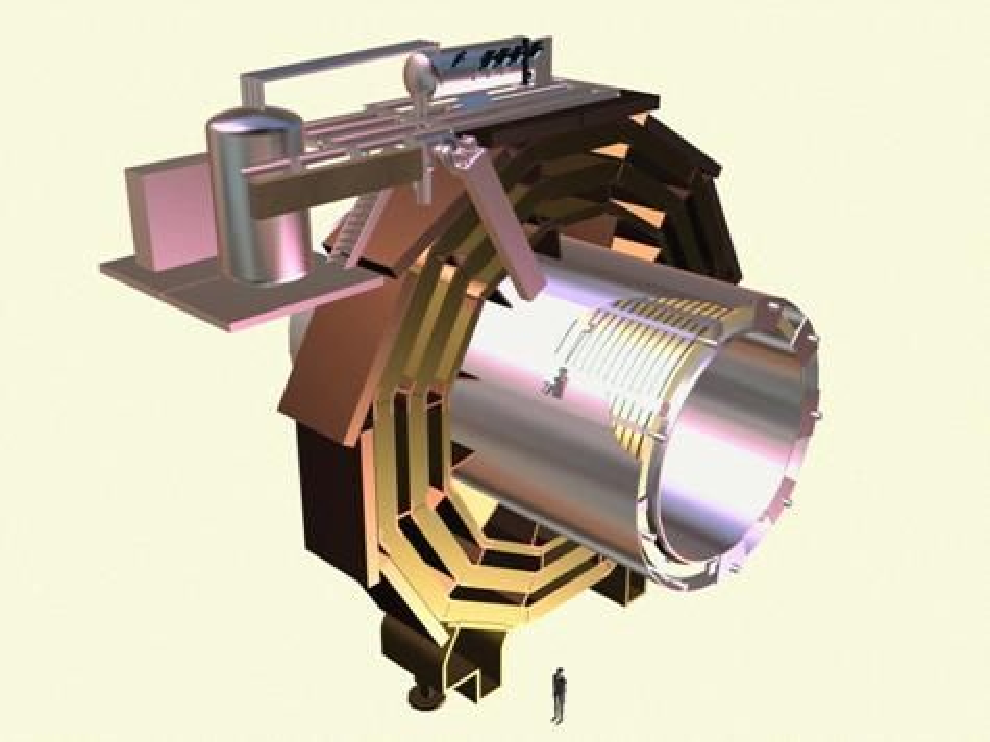
\includegraphics[width=9cm]{Chapter2/CMS_magnet.pdf}
\caption{A schematic view of the solenoidal magnet used in the CMS detector, showing the coil and the central return yoke.}
\label{fig:Magnet}
\end{center}
\end{figure}
%\vspace{-0.3in}

\subsubsection{Muon detector}
The CMS has been specifically designed for precise identification, momentum resolution and triggering of muons within a range $|\eta|$ $<$ 2.4 and $\pt$
$\leq$ 1\unit{TeV}. Muons, though interact electromagnetically,
do not lose much of their energy via bremsstrahlung owing to their high mass as compared to electrons. They interact primarily through ionization loosing
an energy on the average of 1-2$\unit{MeV/g/cm^{2}}$. Due to their less interacting nature, they penetrate the material of ECAL and HCAL, so the muon chambers for their
detection are installed at the very edge of the detector. 

The CMS muon~\cite{muonTDR} system has been divided into four stations interleaved with the return yoke and having a magnetic field of 2\unit{T}.
The barrel muon detector is also longitudinally divided into five wheels labelled as YB0, YB$\pm$1, YB$\pm$2, with each wheel being further divided in the azimuth
direction into 12 sectors of 30$^{^{\circ}}$ each. It uses
three different kind of detectors to observe muons: Drift Tubes (DTs), present in the barrel region upto $|\eta|$ $<$ 1.2; Cathode Strip Chambers (CSCs), present
in the endcap region for 0.9 $<$ $|\eta|$ $<$ 2.4; and Resistive Plate Chambers (RPCs), present in barrel as well as endcaps. Whenever a particle passes through these
chambers, it leaves its signature in the form of hits. Tracking the particle's position in multiple layers and combining the information from tracker, leads to
a precise determination of the position and momentum of the particle. The DTs$/$CSCs are good in position measurements while the RPCs provide
fast response, so a combination
of the three result into a robust muon detector. Diagrams representing the mechanical layout of CMS muon detector and the trajectory of muon through muon stations
is shown in \fig{\ref{fig:CMS_Muon}}.
 
\begin{figure}[h]
\begin{center}
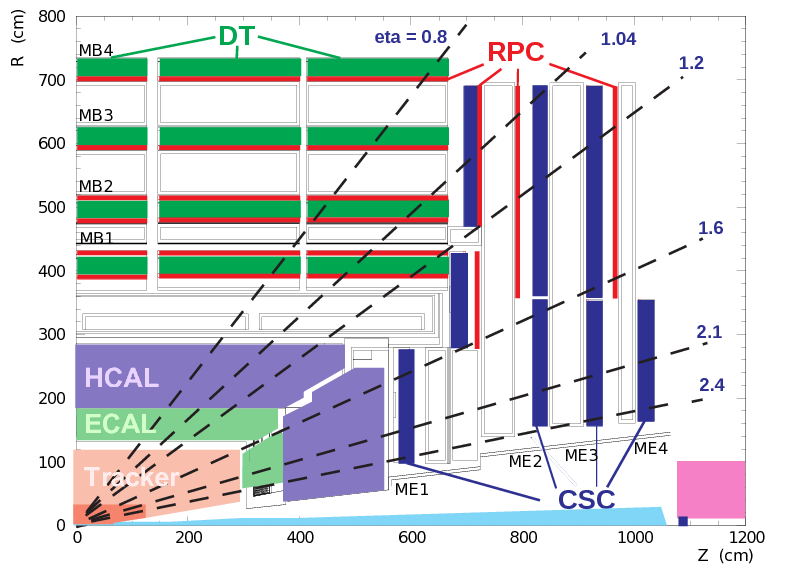
\includegraphics[width=8.5cm]{Chapter2/CMS_MuonDet.png}
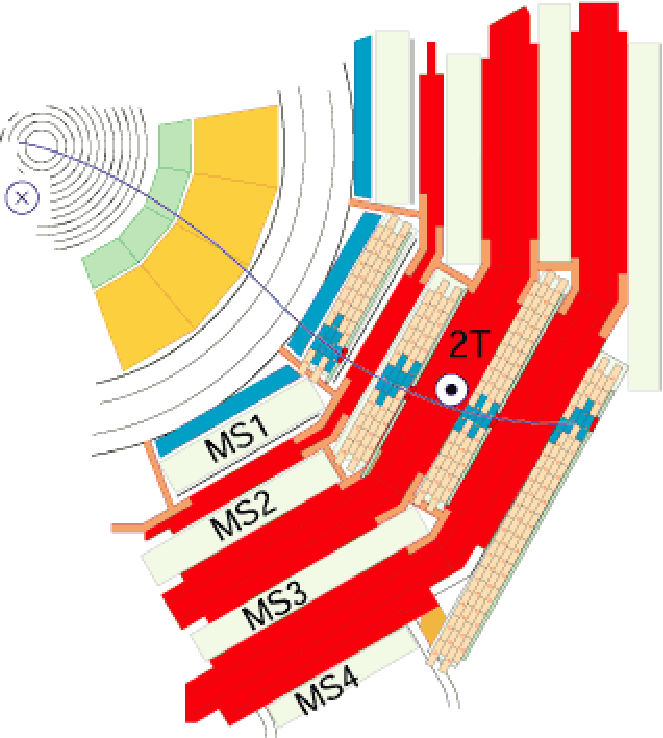
\includegraphics[width=5.5cm]{Chapter2/MuStations.pdf}
\caption{A schematic view of the solenoidal magnet used in CMS, showing the coil and the central return yoke. The trajectory of a muon through the muon stations is also presented.}
\label{fig:CMS_Muon}
\end{center}
\end{figure}
\vspace{-0.3in}

The drift tubes are organized into 4 stations labelled as MB1, MB2, MB3 and MB4, which forms concentric cylinders around the beam pipe.
Each of the inner three stations are composed of 12 drift chambers, with each chamber containing many drift tubes. These chambers are further grouped into
three superlayers denoted as SL1, SL2 and SL3, each consisting of four chambers. SL1 and SL3 provides
the co-ordinates of incident muons in $r-\phi$ plane while SL2 measures the co-ordinates in $r-z$ plane. The outermost station consists of two superlayers only. 
The choice of drift chambers is made in barrel due to the low particle rate and
uniform magnetic field. Each drift tube contains a anode wire of 50$\mu{m}$ diameter and two electrode plates to create electric field. The tube walls
are grounded and act as cathodes. The drift tube is filled with a gas containing a mixture of Ar (85$\%$) and CO$_{2}$ (15$\%$). The voltage difference between
wire and walls is about 1.8\unit{kV}. When a muon pass through the gas volume, it knocks off electrons which travel to the anode wire, carrying along
the information of incident particle. The DTs provide a signal gain of 10$^{5}$ and a drift time of 380\unit{ns}. 

The CSCs have been deployed in the high radiation and uneven magnetic field environment in the endcaps. Owing to their quick response time, high granularity and
radiation hardness, the CSCs are well qualified to identify muons in the range 0.9 $<$ $|\eta|$ $<$ 2.4, overlapping with DTs in 0.9 $<$ $|\eta|$ $<$ 1.2.
The CSC chambers are of trapezoidal shape placed perpendicular to the beam line and cover
10$^{^{\circ}}$-20$^{^{\circ}}$ in $\phi$. These are organized in 4 stations per endcap, labelled as ME$\pm$1, ME$\pm$2, ME$\pm$3 and ME$\pm$4, each station
containing a number of CSCs. Each CSC consists of an array of positive anode wires made of tungsten held perpendicular to the negative cathode strips made of
copper, in a gas mixture of Ar (40$\%$), CO$_{2}$ (50$\%$) and CF$_{4}$ (10$\%$). When a muon enters a CSC, it knocks off electrons from the gas atoms, which then
flock towards the anode wires resulting into an electron avalanche. The positive gas ions move towards cathode strips and induce a charge pulse. Since the
anode wires and cathode strips are present in perpendicular direction, these provide two position co-ordinates corresponding to each particle. This arrangement in
CSCs also results into fast response making them convenient for triggering. Each CSC is composed of six anode wires interleaved with seven cathode strips, providing
the measurements in $r-\phi$ plane. 

The RPCs are parallel plate gaseous detectors with fast response time and adequate position resolution making them suitable for
muon triggering. The RPCs are installed both in barrel (480 chambers)
and endcaps (432 chambers) with two chambers of rectangular shape per DT chamber in barrel and one chamber of trapezoidal shape per CSC chamber in endcaps.
The RPCs have the ability to tag a particle in a time frame much lesser than the bunch crossing time, making them ideal for triggering. The RPC is composed of
two gaps, each operating in avalanche mode and read-out strips are inserted in-between. The total signal induced by the RPC is sum of signal induced in each gap.
However, in order to ensure proper stability and operation of the RPC, an intensive control  of humidity, temperature and pressure is required.  

The muon system of CMS is made up of around 25000$\unit{m^{2}}$ area and more than a million readout channels.
Considering only the muon system without any information from
tracker (stand-alone muon), a momentum resolution of around 9$\%$ is obtained for a muon of $\pt$ $\leq$ 200\unit{GeV}
in low $\eta$ region. For a high $\pt$ muon ($\sim$ 1\unit{TeV}), the resolution varies from 15-40$\%$ for different $\eta$.
Adding tracker information (global muon) results into an improvement in momentum resolution of around 1$\%$ for low $\pt$ muons and around
5$\%$ for high $\pt$ muons. 


\subsubsection{CMS upgrade during Long Shutdown 1}
During LS1 in 2013-2015, minor repair and maintenance work were performed on most of the CMS sub-systems, except for
some major improvements that include: Installation of new pixel tracker layer (explained in \sectn{\ref{Se:CMS_tracker}}) which was actually
done after LS1 and during the technical stop at the
end of 2016, installation of new photo-detectors to improve signal-to-noise ratio in HCAL outer barrel, installation of the fourth RPC disk in the endcap region of
the muon detector which was actually the part of the first CMS technical design report and installation of around 72 new chambers in CSC along with 468 old chambers.
The electronics have also been updated to handle high collision rates.

\subsection{CMS Trigger and Data Acquisition System} \label{Se:CMS_trigger}
Most of the LHC collision data consists of ``soft'' particles which do not participate in any interesting process.
Also, at each bunch crossing, the collisions amount to a raw data of approximately 1\unit{MB}, which at the crossing rate of 40\unit{MHz} (25\unit{ns}), results into
around 40\unit{TB} data per second. It is almost impossible to store and process such a large amount of data.
Therefore, to reduce the data rate while keeping the potentially
interesting events for further analysis, a hardware and software based automated system, referred to as the CMS
trigger system\cite{triggerTDR} has been designed together with a
Data AcQuisition (DAQ) system~\cite{daqhltTDR}, as shown in figure \fig{\ref{fig:CMS_DAQ}}.
The trigger system consists of two layers: a hardware based trigger known as Level-1 (L1) trigger and a software
based trigger known as the High Level Trigger (HLT), reducing the event rate to an average of a few 100\unit{Hz} to
a maximum of 1\unit{kHz}. The data passing through both the trigger levels is stored for offline physics analysis.
In order to obtain the required data rate, sometimes the
triggers are prescaled at L1 or at HLT level, thereby storing only a fraction of selected events.
DAQ acts as a bridge between the two trigger layers, it gathers data from first trigger layer, digitizes and build it and
pass it to second trigger layer.

\begin{figure}[h]
\begin{center}
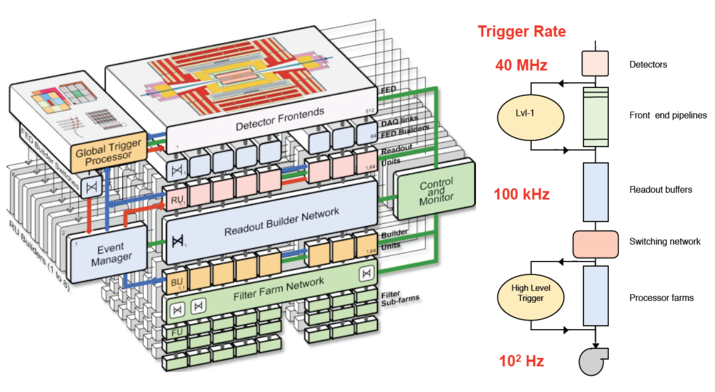
\includegraphics[width=13cm]{Chapter2/DAQsystem.png}
\caption{CMS Data Acquisition and trigger system.}
\label{fig:CMS_DAQ}
\end{center}
\end{figure}
\vspace{-0.3in}

\subsubsection{Level-1 trigger}
The Level-1 trigger of CMS is a set of hardware based triggers that rely on custom electronics. It has been designed to produce an output data
rate limit of 100\unit{kHz}. The L1 triggers are implemented as custom hardware processors and considers only low resolution, coarsely segmented data
from ECAL, HCAL and muon systems while keeping the high resolution data in the pipelined memories present in the front-end electronics. 
The L1 stores data in pipeline for 3.2${\mu{s}}$ during which it transmit its decision to detector electronics. 
The L1 trigger consists of a number of hardware components including field-programmable gate-array (FPGA) technology, ASICs and programmable lookup tables (LUTs).
A block diagram representing the architecture of L1 trigger system is shown in \fig{\ref{fig:CMS_L1}}.

\begin{figure}[h]
\begin{center}
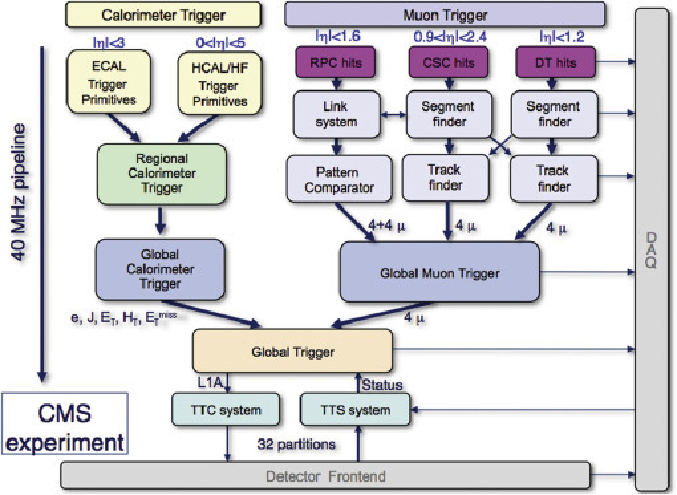
\includegraphics[width=10cm]{Chapter2/CMS_L1_trigger.pdf}
\caption{An architecture of CMS Level-1 trigger system.}
\label{fig:CMS_L1}
\end{center}
\end{figure}
%\vspace{-0.3in}
The L1 trigger consists of local, regional and global components. At the top are the local triggers, also known as Trigger Primitive Generators (TPGs),
which takes the information from the energy deposits in calorimeter towers and hit patterns in muon chambers. The information from TPGs are then passed on
to the regional triggers. The regional calorimeter triggers (RCTs) makes use of this information and forms sorted and ranked trigger
objects like electrons, photons and jets. The regional muon triggers (RMTs) join the segments and complete the tracks along with assigning physical parameters to them.
The regional triggers passes these objects along with various information to the Global Calorimeter Triggers (GCTs) and Global Muon Triggers (GMTs)
which sort out the highest ranked calorimeter and muon candidates along with determining various physics parameters like $\et$, $\met$, number of jets, $\HT$ etc.
This information from GCTs and GMTs are then passed on to the Global triggers (GTs),
the top level entity of L1 hierarchy, which makes the final decision of keeping or rejecting the event
by applying the programmable topological cuts and energy thresholds on the objects and issues the final Level-1 Accept (L1A) decision. The L1A is then
passed on to the Trigger Timing and Control (TTC) system for transferring it further to the detector front-end, from where it goes into the DAQ system.
The TTC also interfaces with the LHC machine to
provide clock and orbit information. The GT sends a command by the use of TTC in order to keep all the detectors and their electronics well in synchronization.

\subsubsection{High level trigger}
The CMS high level trigger accepts the output of L1 trigger and process it further by using a software (written mostly in C$++$)
based trigger system implemented in a filter farm consisting of more than thousand commercial processors. All major aspects of offline reconstruction code
are included in the filter farm software and is designed to reduce data rate to a minimum of few 100\unit{Hz}.
The average time taken in HLT processing is around 100\unit{ms}.
It employs the use of high resolution data and utilize many sophisticated algorithms to identify interesting events for
further storage. The HLT is based on highly flexible programming environment such that
the changes in the algorithms can be easily done to improve the various selections and to deal with unexpected experimental conditions.  
A set of algorithms that reconstruct the physics candidates (known as producers) and apply various selections to the reconstructed objects
(known as filters) is known as a ``trigger path''; a number of trigger paths together constitute a ``HLT trigger menu''.
Within a trigger path, the various algorithms are arranged in an increasing order of complexity, with the most complex algorithms like the b-tagging, are executed 
in the end. Events that pass any of the trigger paths within a trigger menu are considered for further analysis and are sent to storage manager where
these are stored on disks and are sent to CMS Tier-0 system present at CERN for offline processing and permanent storage.

\subsubsection{Data acquisition system}
The CMS DAQ mainly work as a carrier that gathers the data stored in detector's front-end modules at the Level-1 accept rate
and deliver it to HLT filter farms for further processing. 
It operates at an input data rate of 100\unit{kHz}, the output rate of L1 trigger. The complete processing of DAQ is summarized as follows:
First of all, the front end systems (FESs) store data continuously in 40\unit{MHz} pipelined buffers. As the synchronous L1 trigger comes, data are extracted
from FES via TTC and pushed into front end drivers (FEDs). The FEDs digitize, convert and zero suppress the data and then transfer it to
front end read out links (FRLs) that merge data from different FEDs. These FRLs are known as event builders as these built a complete event by assembling
the event fragments from all FEDs belonging to same L1. The data from FRLs are then transmitted into filter units (FUs). The HLT is mounted over FUs and use
its computing power to perform its operations. These FESs, FEDs, FRLs, FUs all forms the different parts of DAQ system. A Trigger-Throttling System (TTS)
has also been designed to protect DAQ against any back-pressures. 
\subsection{CMS data management}
The raw data after passing the various triggering stages, is managed further by the use of the LHC computing grid~\cite{Eck:840543}.
The grid is constituted of four levels$/$tiers, referred to as Tier-0 (T0), Tier-1 (T1), Tier-2 (T2) and Tier-3 (T3).
Each tier consists of a number of computer facilities and provides a set of dedicated services. 
The Tier-0 is the data center present at CERN, it contributes less than 20$\%$ of total grid computing capacity but it is responsible for maintaining a full copy
of raw data, for performing calibration and prompt reconstruction (prompt-reco) and for distributing the raw and prompt-reco data to Tier-1 centers. 
Tier-1 is a group of around 13 computer centers located in various part of the world and
joined together via optical-fibre links operating at a speed of 10$\unit{gigabytes/sec}$.
The T1 centers together maintain a second copy of raw
data, produce various Monte Carlo (MC) samples\footnote{simulated data samples, more information provided in \chap{\ref{ch:chapter3}}}
and re-reconstruct the raw data along with distributing it to various Tier-2 centers.
The T2 centers are the sites where physicists can log-in and perform their analysis within the CMSSW environment. These centers also produce the MC samples
and share them with T1 centers for storage and distribution to other sites. There are around 155 T2 sites distributed all over the world. 
The Tier-3 consists of local computing resources at various universities and institutes which individual users can access from any place around the world using grid,
and can use for storage and data analysis. 

The data present at various tiers are managed by the use of three data management tools~\cite{Giffels:2014tfa}:
Physics Experiment Data Export (PhEDEx)~\cite{Egeland:2008zz, Egeland:1196164}, Data Bookeeping Service (DBS)~\cite{Afaq:2007zz}
and Data Aggregation Service (DAS)~\cite{KUZNETSOV20101535}. The PhEDEx service provides data information access through the central PhEDEx database,
perform operations such as requesting data transfer or data deletion and transport the data among the different CMS sites along with keeping a track.
The DBS service keeps a metadata catalog of all the CMS data used by physicists as well as
the various production and analysis systems. The DAS service provides the user an overview of all the available datasets and keep a mapping between the datasets
and corresponding file blocks.
\subsection{CMS software and computing}
The CMS physics analyst perform various analyses using a collection of softwares based on C$++$ and python, referred to as the ``CMS Software frameWork''
(CMSSW)~\cite{cmsTDR}, installed at various T2 and T3 centers.
A number of services including simulations, calibration corrections or reconstruction etc. are supported by this framework.  
It consists of one main executable, known as cmsRun, along with many other plug-in modules, containing all the required codes for event processing.  
The cmsRun operates over a python configuration file that contains all the important information regarding the data and modules. 
The CMSSW software has been built over the concept of an ``Event''. An Event contains the information of a particular collision in different data
formats, a physics dataset consists of many events and are stored in the form of ROOT\footnote{ROOT is a data analysis framework}~\cite{Brun:1997pa} files.
A RAW data format contains the output of online trigger decisions and has a size of 1.5$\unit{MB}/$event, the size of RAW data in a simulated sample
is around 2$\unit{MB}/$event due to additional information. A RECO data
format contains the offline reconstructed data that includes the high level physics objects such as electrons, photons, jets, b-jets, muons, taus $\met$ etc., in
convenient format and has a size of 250$\unit{kB}/$event. Usually, a RECO data format contains a large amount of unwanted information,
so more compact data formats are obtained by filtering the RECO data. These data formats
includes Analysis Object Data (AOD) and mini Analysis Object Data (mini-AOD), used in almost all physics analyses. 

%It along with ATLAS chase the same physics goals but with the use of different technology as can be seen in \tab{\ref{Table:CMS_ATLAS_Comp}}. 
%\begin{table}[h!]
\begin{center}
\resizebox{16cm}{!}{
%\begin{tabular}{c !{\vrule width -1pt}c !{\vrule width -1pt}c !{\vrule width -1pt}c !{\vrule width -1pt}c !{\vrule width -1pt}c !{\vrule width -1pt}c !{\vrule width -1pt}c}  %%% !{\vrule width -1pt} to make column line width less, so that white space not visible in colored table. but not working very nicely.
\renewcommand{\arraystretch}{1.2}
\begin{tabular}{lcc}
\toprule
\belowrulesepcolor{Mygray}
\belowrulesepcolor{Mygray}
\belowrulesepcolor{Mygray}
\rowcolor{Mygray}[\dimexpr\tabcolsep+0.09pt\relax]  
System  & CMS & ATLAS \\
\aboverulesepcolor{Mygray}
\aboverulesepcolor{Mygray}
\aboverulesepcolor{Mygray}
\midrule
\bf{Tracker} & Silicon (pixel + microstrip) & Silicon (pixel + microstrip) \\
&                              & Gas (transition radiation) \\
\midrule
\bf{Electromagnetic} &  PbWO$_{4}$ crystals & Sampling (lead/liquid argon) \\
\bf{calorimeter} & &  \\
\midrule
\bf{Hadron} & Sampling (brass/plastic scintillator) & Sampling (steel/plastic scintillator) \\
\bf{calorimeter} &                                       & (copper/liquid argon) \\
\midrule
\bf{Muon detector} & Gas & Gas \\
\midrule
\bf{Magnet}      & Solenoid (around tracker        & Solenoid (around tracker)  \\
                 & and calorimeters)  &  Toroid (around muon)\\
&      Iron return yoke                      &  \\
\midrule
\bf{Magnetic field} & Approximately 4\unit{T} in solenoid & Approximately 2\unit{T} in solenoid \\
               & and 2\unit{T} in return yoke        & and 0.5--1\unit{T} in toroid \\
\bottomrule
\end{tabular}
}
\caption{A comparison of the technologies used in CMS and ATLAS.}
\label{Table:CMS_ATLAS_Comp}
\end{center}
\end{table}
\vspace{-0.4in}




\clearemptydoublepage
\chapter{Event Reconstruction And Simulation}\label{ch:chapter3}
The detector provides information about the collisions and the underlying physics processes in the form of various electronic signals.
A number of steps have to be followed in order to obtain a meaningful physics result,
by making use of scientific and theoretical knowledge, computing and man-power. A diagrammatic representation of an event processing chain
in presented in \fig{\ref{fig:EvtChain}}.

\begin{figure}[h]
\begin{center}
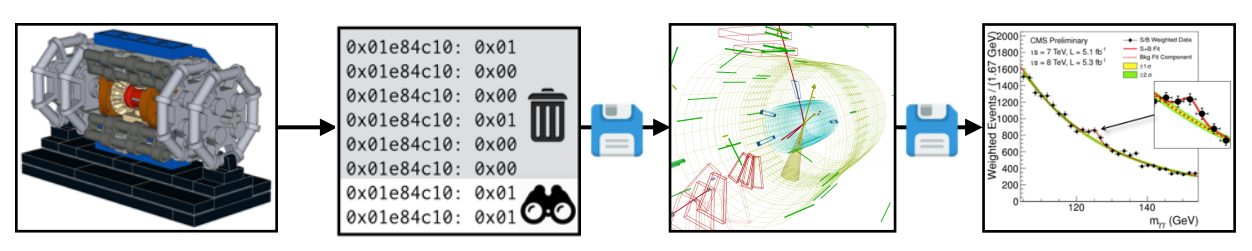
\includegraphics[width=15cm]{Chapter3/Event_reco_chain.png}
\caption{A diagrammatic representation of an event processing chain.}
\label{fig:EvtChain}
\end{center}
\end{figure}
\vspace{-0.2in}

The electronic signals from various sub-detectors are stored, after digitization, in the form of RAW data using online trigger and DAQ system.
This RAW data is further processed using a software based multi-level process, known as ``Event Reconstruction''~\cite{Lange:2011zza}, that refines the data,
applies various calibration corrections and construct high-level physics objects\footnote{High-level physics objects are the reconstructed particles like photons,
  electrons, muons, taus etc.}. At CMS, two levels of reconstruction are performed, one is a fast reconstruction, known as prompt reconstruction, done alongwith
the data collection by using less time consuming algorithms and the second one is a detailed reconstruction, known as re-reconstruction, performed at a later time.
The reconstructed data is written in various data formats (e.g. RECO, AOD, mini-AOD)
that differ in size, technicalities, compactness etc.

Based on the theoretical knowledge, it is possible to simulate the behaviour of various particles within the detectors using event generators, also
called Monte Carlo (MC) generators~\cite{Buckley:2011ms, Dobbs:2004qw}. Event generators make use of some computer programs based on Monte Carlo
techniques~\cite{MC_Tech} to generate physics events corresponding to different physics processes. This simulated data form an integral part of
any physics analysis, used in determining various SM parameters, validating$/$rejecting any new theory, forming expected background for experimental data,
evaluating various uncertainties and trigger parameters etc. In the language of statistics, it forms the null hypothesis for the test of any new theory. 
The simulated data is also written in different data formats like RECOSIM, AODSIM, mini-AODSIM, in correspondence with reconstructed data.

This chapter details the different steps and procedures used in the reconstruction and simulation of the events for CMS physics analyses.
\section{Event Reconstruction}
Reconstruction is the process of constructing physics quantities using the raw data collected from the experiment. 
Inside the CMS detector, starting from the collision point, the particles first arrive in the tracker where the charged particle's trajectories, their momenta and
interaction points are reconstructed using the particle's signal and bending angle in the sensitive layers of tracker. If the particle is either electron or photon,
it will be absorbed in ECAL. The EM showers generated by such particles are detected as energy clusters in ECAL cells and are used in the determination
of energy and direction of these particles. Hadrons (charged and neutral) will be absorbed in HCAL, sometimes initiating their showers in ECAL.
The associated clusters are used in measuring the energies and directions of hadrons. Only muons and neutrinos pass through the calorimeters with negligible interactions.
While neutrinos escape unidentified, muons leave their signature in muon detectors, used to reconstruct the muon direction and momentum.
This behaviour of different particles is graphically depicted in \fig{\ref{fig:CMS_slice}} in a slice of CMS detector.

\begin{figure}[h]
\begin{center}
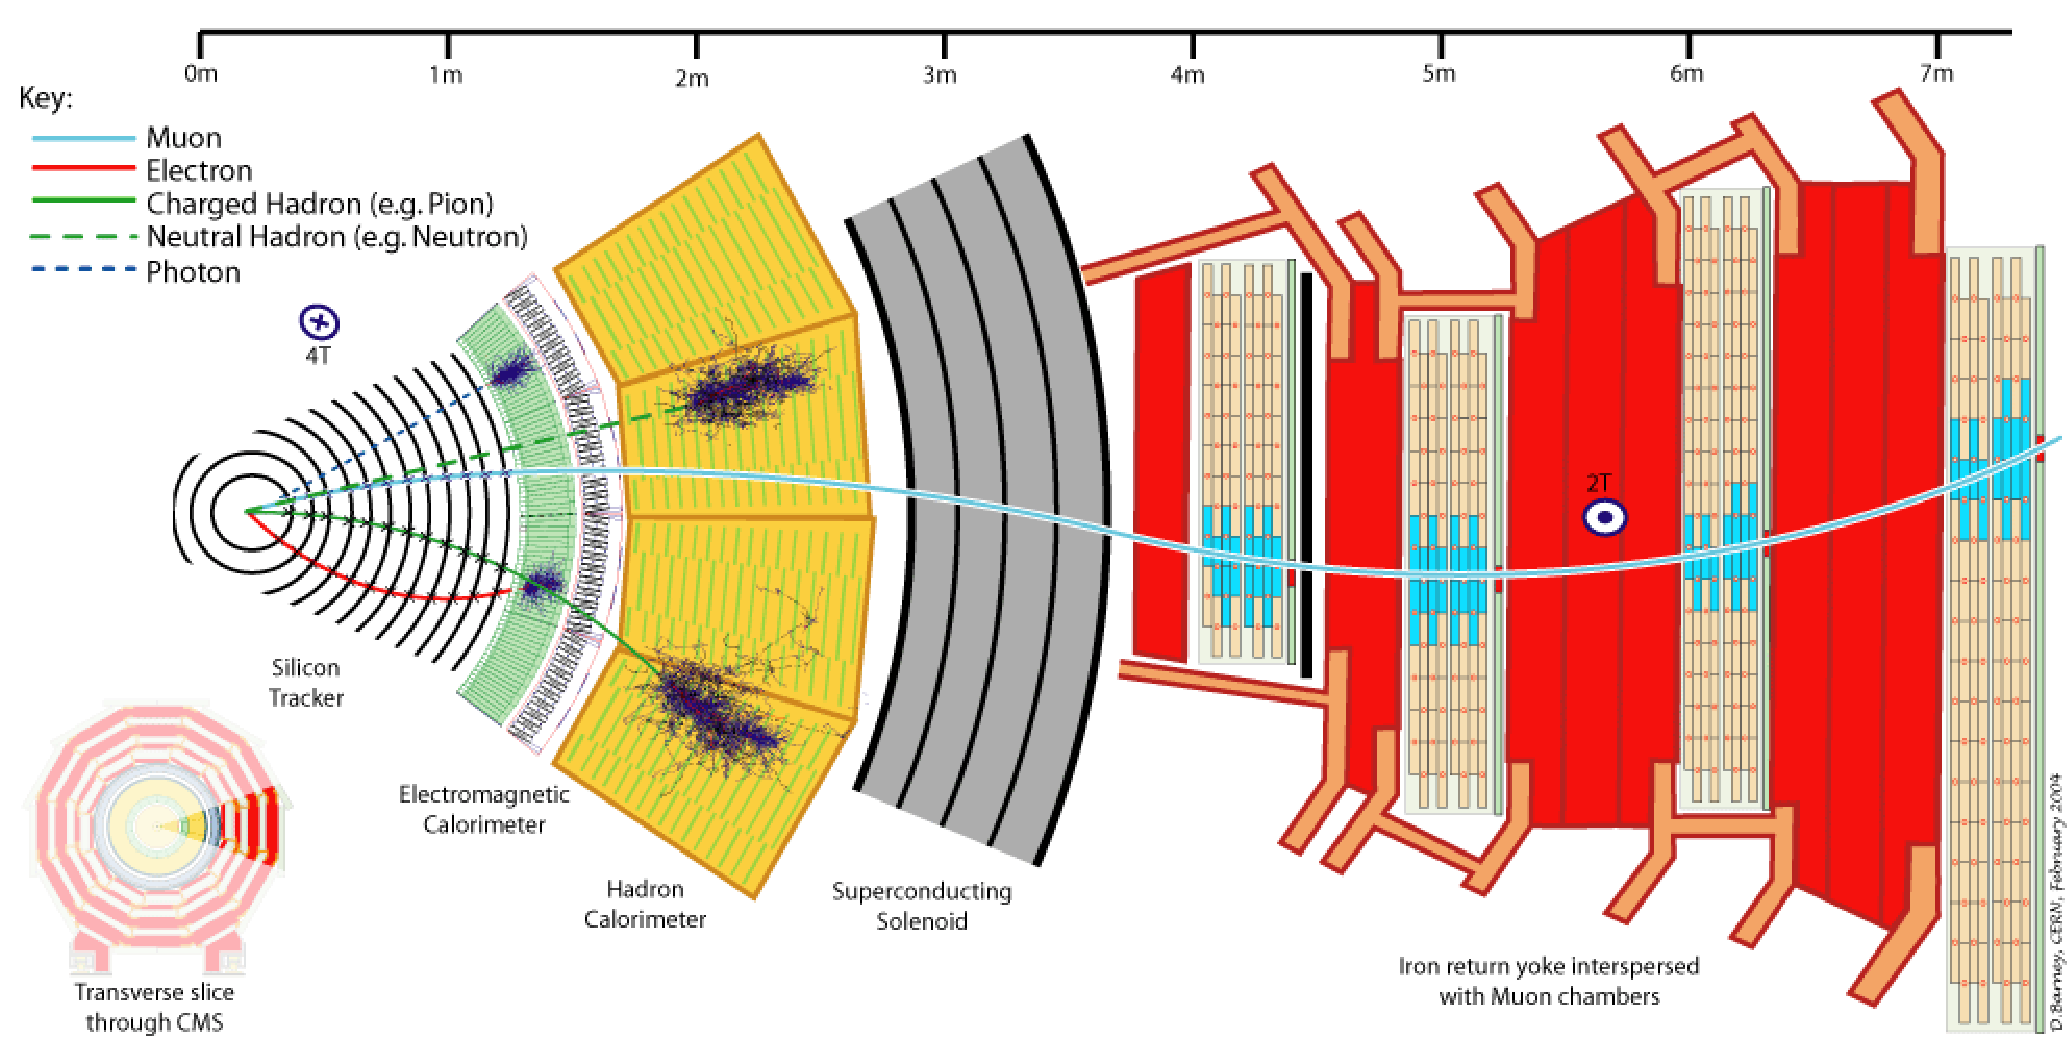
\includegraphics[width=14cm]{Chapter3/CMS_Slice.pdf}
\caption{A graphical representation of the trajectories of various particles through the CMS detector.}
\label{fig:CMS_slice}
\end{center}
\end{figure}

The CMS reconstruction software~\cite{Lange:2011zza} is a collection of several independent units, each consisting of many reconstruction algorithms
and provides one set of reconstructed objects at the output. The software has been developed and validated by making use of simulated data.
The complete reconstruction process is divided into three steps as shown in \fig{\ref{fig:CMS_reco_steps}}. 

\begin{figure}[h]
\begin{center}
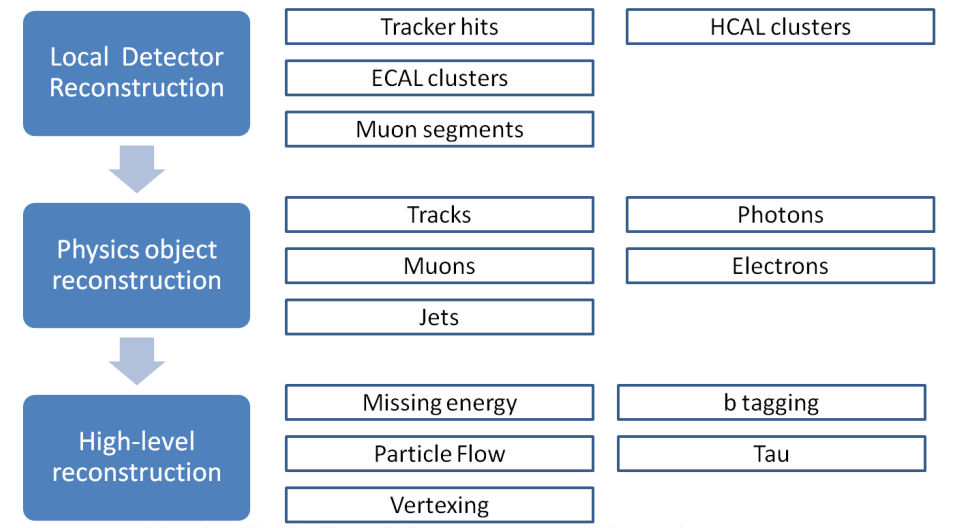
\includegraphics[width=12cm]{Chapter3/CMS_Reco_steps.png}
\caption{Different steps of CMS reconstruction program.}
\label{fig:CMS_reco_steps}
\end{center}
\end{figure}
\vspace{-0.2in}
At first, the local reconstruction takes place within a particular detector module of a sub-detector.
It uses raw data as input and provide in output the reconstructed units,
also called rechits. These rechits are corrected for any uncertainties by the application of different calibration corrections. 
The form of these rechits depends on the sub-detector under consideration. These are the position measurements inside tracker and muon system while
energy clusters inside the calorimeters. These reconstructed hits act as input to the next reconstruction level, known as global reconstruction
where the physics object reconstruction takes place. At this level, the information obtained from different detector modules within a sub-detector
is combined to form sub-detector level objects, like high$/$low $\pt$ charged particle tracks and displaced vertices in the tracker,
candidate muon tracks in the muon system, photon/electrons in ECAL and jets in ECAL$+$HCAL.
These objects from different sub-detectors are then combined to reconstruct high-level physics analyses objects
using an optimally efficient Particle Flow (PF) reconstruction algorithm~\cite{Sirunyan:2017ulk},
as a final stage of event reconstruction. 
The high-level objects like $\met$, tau, b-tagging $\etc$ that require the additional knowledge of
tracks, displaced vertices, $\sum{\pt}$, are also reconstructed at this level. 

Since this thesis is based on an analysis that requires a photon and a jet or a b-jet in the final state, so only the steps needed to reconstruct photons and
jets (b-jets) are considered in detail in the following sections.

\subsection{Track reconstruction}
The tracker is the first detector in which the charge particles leave their signatures, hence reconstruction of tracks is one of the most important task of
the CMS reconstruction program. More than a thousand particles pass through the tracker every 25\unit{ns}, thereby, making the track reconstruction
immensely challenging. The track reconstruction is a combinatorial kind of problem, as for a partial track formed by hits in the internal layers, there can be many
compatible hits forming different tracks in the outer layers, so the reconstruction algorithm should be able to properly locate the equitable hits without
loosing any tracks, over a broad range of $\pt$ from 100\unit{MeV} to 1\unit{TeV}. This insurmountable feat is achieved by the use of the
``Combinatorial Track Finder'' (CTF)~\cite{Chatrchyan:2014fea,Adam:934067} algorithm which is an extension of the
Kalman filter~\cite{Fruhwirth:1987fm, Billoir:1989mh, Billoir:1990we} algorithm, an algorithm that allows single framework
modelling of complete track reconstruction program. 
 
At first, the individual hits in pixel and strip tracker are reconstructed at the local reconstruction level by clustering the
zero-suppressed\footnote{Zero-suppression is the default noise cleaning performed in CMS detector, in which all signals below a particular threshold
are rejected, the value of the threshold depends on the sub-detector part under study.} signals passing
the specified thresholds. The corresponding hit positions and associated uncertainties are also estimated with an average efficiency of more than 99$\%$.  
These hits are then used as input into the CTF algorithm to reconstruct the charged particle tracks and their position$/$momentum. The CTF algorithm is based on
a process known as ``iterative tracking'' that reconstruct the track collection in a number of iterations. The basic idea is to first sort out the easily accessible
tracks, like the high $\pt$ ones near the interaction region and do not consider the hits corresponding to these tracks in the next iterations, thereby,
successively reducing the complexity of subsequent iterations. This strategy is very useful in building up of more difficult tracks,
like low $\pt$ or displaced tracks. The algorithm has a total of $6$ iterations, starting with iteration $0$, that reconstruct the prompt tracks
(close to pp interaction point) with $\pt$ $>$ 0.8\unit{GeV} and having at least three pixel hits.
Iteration $1$ takes care of all other high $\pt$ prompt tracks with two pixel hits. Iteration $2$ has been configured to locate low $\pt$ ($\pt$ $\le$ 0.8\unit{GeV}) prompt
tracks. Lastly, the iterations $3-5$ are intended to recover tracks originated outside the luminous region of pp interactions and not considered in previous iterations.
The first three iterations of CTF has a prompt track reconstruction efficiency of $\sim$ 90$\%$ for charged hadrons and $\sim$ 99.5$\%$ for muons, the
efficiency for hadrons deteriorate due to their nuclear interactions with the tracker material. The track reconstruction is the most CPU extensive
task with each iteration step constituted of four further steps as detailed below:
%\vspace{-0.1in}
\begin{itemize}[leftmargin=*]
\item {\bf{Seed generation}}: In this step, the track seeds are generated using the hits in the internal pixel layers of tracker. A set of parameters are used to determine
  the compatible hits that has the capability of track formation. Usually, a window around a hit in a layer is used to find the compatible hit in the adjacent layer.
  A seed provides an initial estimate of track parameters and their associated uncertainties. The seed generation algorithm requires the knowledge of
  center of beam spot and location of primary vertices including the ones coming from pileup events. Since the charged particles traverse a helical path under the effect
  of the uniform magnetic field, a minimum of five parameters are required to define a trajectory.   
\item {\bf{Pattern recognition/track finding}}: The track seeds originating in the first step are used to determine the complete track by looking for other hits in the
  outer pixel and strip layers. The corresponding algorithm is based on the Kalman filter technique~\cite{Fruhwirth:1987fm, Billoir:1989mh, Billoir:1990we}
  that makes use of coarsely estimated track parameters by
  the trajectory seed. As it finds new hits in successive layers, it keeps on updating the track parameters. A $\chi^{2}$-test is performed to check the
  compatibility of hits with the extrapolated trajectory.   
\item {\bf{Track fitting}}: The candidate track estimated by the pattern recognition can be biased by the constraints applied to the trajectory at the
  seeding step. Therefore, the trajectory is fitted again by initiating a Kalman filter from the innermost hit and proceeding iteratively through all the hits
  in the outward direction, the track parameters are updated sequentially at each hit. The covariance matrix corresponding to the fit has been scaled by a large
  factor to avoid any biases. This filter is then followed by a smoothing step, in which a second
  filter is initiated in the outermost hit using the results obtained by the first filter and proceeds backwards toward the beam-line. The final track parameters
  are then obtained by the weighted average of the two filters. In order to get best precision, a Runga-Kutta propagator is used to extrapolate the
  trajectory. The $\chi^{2}$ approach is also followed to check the presence of and removal of any spurious hits (outliers), that do not belong to the track.
\item {\bf{Track selection}}: In the high luminosity environment of LHC, there is a significant probability of reconstructing fake tracks (tracks not associated with
  charged particles). So track selection step imposes some quality requirements on the reconstructed tracks to reduce the fraction of fakes,
  these quality checks include the requirements on the number of hit layers in the track, the $\chi^{2}/$d.o.f. of the track fit,
  the impact parameters of track in transverse and longitudinal directions and the compatibility with the primary vertex.
  A track is considered as a final track candidate if it passes these quality criteria.
\end{itemize}
\subsection{Vertex reconstruction}
The vertex reconstruction~\cite{Chatrchyan:2014fea} involves determination of all the
pp interaction vertices in an event, coming from the signal as well as the pileup collisions. 
The algorithm is constituted of three steps, which include the track selection, clustering of the tracks that seem to be originating from the same interaction point
and fitting of the tracks to locate the vertex position.

The track selection step sort out the prompt tracks that are appeared to be produced in the primary interaction region by requiring the maximum transverse
impact parameter significance relative to the beam spot~\cite{Miao:2007zz} position to be $<$ 5, more than 2 pixel or more than 5 pixel$+$strip hits and normalized
$\chi^{2}$ from the trajectory fit to be $<$ 20. No requirements are imposed on track $\pt$ in order to ensure high reconstruction efficiency.
The clustering of the selected tracks is done by the use of a deterministic annealing (DA) algorithm~\cite{DAC_mech} which 
considers the z-coordinates of the tracks at the point of closest approach from the center of beam spot and their
corresponding uncertainties. This algorithm considers many prototype vertices initially and assign a number of vertices to each track with different weights
which reflects the track consistency to be coming from the beam spot.
A priori, each of the configurations is considered to be equally likely. A $\chi^{2}$ minimization 
is performed to obtain the most probable vertex corresponding to each configuration which finally results into a number of effective vertices at distinct positions.  
\subsection{Photon reconstruction and identification}
Photons are one of the most abundant particles produced in pp collisions either as the direct products of pp interactions (known as prompt or signal photons)
or as the decay products of other particles. These, along with electrons, are detected and reconstructed using ECAL signals.
A detailed description of the procedure used has been provided as follows.
\subsubsection{Photon reconstruction}
Photons are absorbed in ECAL by depositing their energies, 
in the form of showers of secondary particles, in a number of ECAL crystals. The energy reconstruction of photons
takes place by grouping the energy depositions in different crystals in the form of clusters and superclusters (clusters of clusters).
If no material is present between the collision point and the calorimeter, then
electrons$/$photons deposit around 97$\%$ (94$\%$) of their energy in 5$\times$5 (3$\times$3) crystal matrix. But the presence of tracker in-between, results
into showering even before reaching ECAL, with a spread in $\phi$ direction arising due to the effect of magnetic field. 
Similar reconstruction algorithms are used for both electrons and photons; electrons also use further directional information from the tracker. 

The photon reconstruction~\cite{Khachatryan:2015iwa, Anderson:1365024} in CMS takes place in a number of steps
illustrated in the \fig{\ref{fig:ECAL_Reco}}. The first step
is the local reconstruction and calibration of EcalRecHits. This is then followed by a second step that involves clustering of various rechits to form energy clusters
and superclusters. The third and final step considers the energy scale correction to the reconstructed superclusters.
These steps are explained one by one in the coming sections.

%\vspace{-0.2in}
\begin{figure}[h]
\begin{center}
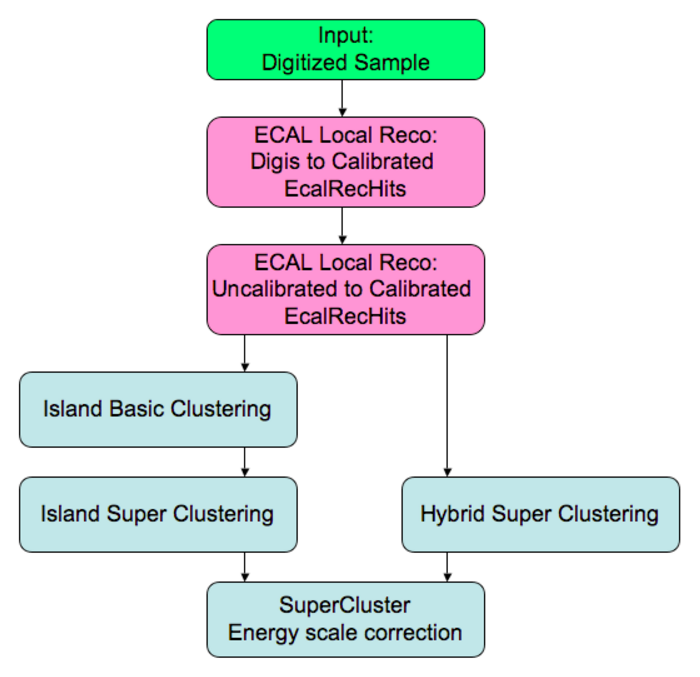
\includegraphics[width=10cm]{Chapter3/ECAL_Reco.png}
\caption{Various steps followed in reconstruction of particles inside ECAL.}
\label{fig:ECAL_Reco}
\end{center}
\end{figure}
\vspace{-0.3in}

\paragraph{Calibration of Ecal channels}\label{para:Calib}
\hspace{\parindent} The e$^{-}/\gamma$ signals in ECAL are calibrated and corrected to account for a number of detector effects~\cite{Chatrchyan:2013dga}.
The ECAL crystals have a tendency to degrade light response if illuminated continuously for a long time, therefore, the transparency of these crystals is
monitored during data taking by using a synchronous laser system and the observed changes are corrected for individual crystals during event reconstruction.
The relative calibration of individual channels is done by deploying the knowledge of $\phi$-symmetry of various energy depositions, the invariant mass of
$\pi^{0}/\eta$ mesons in diphoton channel and the momentum measurement of electrons, coming from decays of W$^{\pm}$ and Z bosons, in tracker.

\paragraph{Clustering}
\hspace{\parindent} The clustering algorithms group together the crystals associated with different electromagnetic showers into clusters.
Since the showers have a spread in $\phi$-direction due to the magnetic field, the clusters which
are close in $\eta$-direction are further grouped together into superclusters using a larger $\phi$ window.
Due to different crystal geometries in ECAL barrel and
endcap, two different algorithms, namely, Hybrid algorithm in barrel and Multi5$\times$5 (a modified island) algorithm in endcap, described in detail below are used. 

\vspace{-0.2in}
\begin{itemize}[leftmargin=*]
\item {\bf{Hybrid algorithm}}: The hybrid algorithm is a super-clustering algorithm deployed in the ECAL barrel that makes use of the $\eta-\phi$ geometry of crystals
  and the corresponding knowledge of lateral shower shape in $\eta$-direction to construct superclusters of electron and photon energy deposits.  This algorithm
  considers fixed length window in $\eta$ while variable length window in $\phi$-direction. An illustration of the algorithm has been provided in \fig{\ref{fig:Hybrid}}.
  
  \begin{figure}[h]
  \begin{center}
  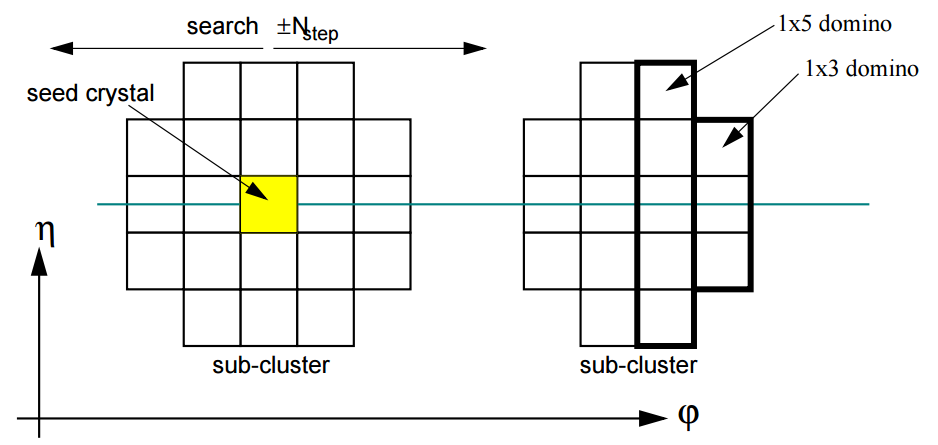
\includegraphics[width=13cm]{Chapter3/PhReco_hybrid_algo.png}
  \caption{An illustration of the Hybrid algorithm used for clustering in ECAL barrel region.}
  \label{fig:Hybrid}
  \end{center}
  \end{figure}
  \vspace{-0.2in}
The complete step-by-step procedure is outlined as follows:
  \begin{enumerate}
  \item Start by searching for a seed crystal, that is the maximum energy crystal satisfying $E_{\textrm{T}}$ $>$ $E_{\textrm{T,seed}}^{\textrm{thres}}$
    (1\unit{GeV}). The crystal should not belong to any other cluster. Terminate the process in case no such crystal is found.
  \item Construct a 1$\times$3 domino of crystals in $\phi-\eta$ direction. If $E_{\textrm{domino}}$ $>$ 0, then extend it to a 1$\times$5 domino. Add other 1$\times$5
    dominoes to it by moving in $\phi$-direction on either side of seed domino upto $\pm$N$_{\textrm{step}}$ crystal length in $\phi$ where N$_{\textrm{step}}$ = 17.
    If energy of a domino falls below $E_{\textrm{domino}}^{\textrm{thres}}$ (0.1\unit{GeV}), do not consider it.
  \item Group the selected adjacent dominoes into local energy clusters. If energy of a local cluster falls below $E_{\textrm{cluster}}^{\textrm{thres}}$ (0.35\unit{GeV}),
    then remove the corresponding dominoes from the final supercluster. 
  \end{enumerate}
\item {\bf{Multi5$\times$5 algorithm}}: Since the geometry of crystals in ECAL endcap is not the same as in the barrel, a different algorithm named Multi5$\times$5
  has been utilized in endcaps to collect the energy deposits within a window in $\eta-\phi$ plane.
  The Multi5$\times$5 algorithm first naively creates the basic clusters and then group them together into superclusters on the basis of their proximity in $\eta/\phi$
  direction. The complete description of the procedure is provided as follows:
  \begin{enumerate}
  \item At first, the seed crystals that do not belong to any cluster and that satisfy  $E_{\textrm{T}}$ $>$ $E_{\textrm{T,seed}}^{\textrm{thres}}$,
    required to be equivalent to 0.18 \unit{GeV}, are selected. Terminate the process if no such seed is found.
  \item The seeds are required to be local maxima when compared to the four direct neighbours. If this is not the case, repeat the previous step again.
    Arrange all the seeds in descending order of $E_{\textrm{T}}$.
  \item Start with the highest $E_{\textrm{T}}$ seed and move towards the lower ones while constructing 5$\times$5 crystal matrices around each.
    In this process, do not include the crystals in a matrix that have already been clustered in a previous matrix. The matrices in Multi5$\times$5 algorithm
    can partially overlap with each other
    but the crystals will only belong to the one with high $E_{\textrm{T}}$ seed. The overlapping
    matrices represent the close showers due to bremsstrahlung etc.
\item In order to construct a supercluster, all the 5$\times$5 clusters whose total energy satisfies, $E_{\textrm{T,cluster}}$ $>$      
  $E_{\textrm{T,cluster}}^{\textrm{min}}$ (1\unit{GeV}), are considered within a search road in $\eta$ and $\phi$ around each seed having the range $\eta\pm\Delta\eta$
  and $\phi\pm\Delta\phi$ where $\Delta\eta$ = 0.07 and $\Delta\phi$ = 0.3\unit{rad}. An illustration of this is presented in \fig{\ref{fig:Multi5x5}}.
  \end{enumerate} 
  \begin{figure}[h]
  \begin{center}
  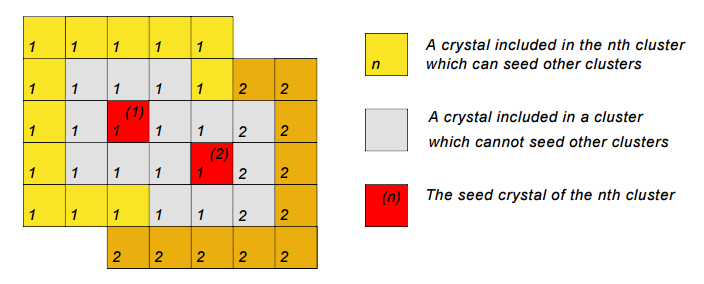
\includegraphics[width=11cm]{Chapter3/PhReco_multi5x5_algo.png}
  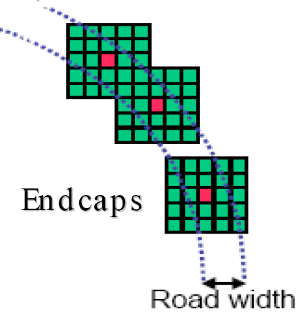
\includegraphics[width=4.5cm]{Chapter3/Multi5x5_road.png}
  \caption{An illustration showing overlapping of two Multi5$\times$5 clusters. Clusters in yellow are eligible to seed other Multi5$\times$5 clusters if
    they form the local energy maxima. The mechanism of formation of a supercluster using many multi5$\times$5 clusters is also shown.}
  \label{fig:Multi5x5}
  \end{center}
  \end{figure}
\end{itemize}
\vspace{-0.2in}

Since the pre-shower detector is present in front of ECAL endcaps in the $\eta$ range 1.65 $<$ $|\eta|$ $<$ 2.6, the particles deposit a fraction of their energy in the
pre-shower before reaching the endcap. In order to obtain this energy, the energy weighted positions of all the 5$\times$5 clusters belonging to a supercluster
in endcap are taken and extrapolated to the preshower planes, while taking the most energetic cluster as reference point.
The maximum distance between the clusters and the
reference point in $\phi$, along with an extension of $\pm$0.15\unit{rad}, is taken as the pre-shower clustering range in $\phi$. The corresponding range in $\eta$ has been
set to $\pm$0.15. The energy deposited in pre-shower in this range is computed and added into the endcap supercluster energy.

Each supercluster corresponds to a potential photon candidate.
The position of a supercluster in all the clustering algorithms is estimated via an energy weighted average of the positions of all the crystals belonging to the
supercluster. Each crystal is assigned a weight equivalent to, $w_{i} = max(0,4.7\,+\,\ln(E_{i}/E_{SC}))$~\cite{Meschi:687345}.
The supercluster position is then connected to the primary vertex of the event to obtain a direction of photon's momentum.
If many primary vertices exist in an event, then the one with highest track sum ${\ptx{2}}$ is considered.

\paragraph{Energy scale corrections of superclusters}
\hspace{\parindent} There are many factors that affect the resolution of the energy measured in ECAL using clustering algorithms.
These mainly include the energy losses due to the bremsstrahlung and photon conversions in the material of the tracker, leading to an underestimation of the energy.
The aim of supercluster energy corrections is to compensate for various energy losses and achieve a homogeneous response throughout the ECAL.\
The corrected energy of a reconstructed particle in ECAL is given by
\begin{equation}
E = F\times{G}\times\sum_{\textrm{cluster}}c_{i}\times{A_{i}}
\end{equation}
where $A_{i}$ refers to the signal amplitude given by the ADC counts; $c_{i}$ is the inter-calibration term that equalizes the different crystal's response
(as discussed under~\ref{para:Calib});
$G$ is the scale representing the global correction term defined such that the product of $G$ and energy amplitude of a $5\times5$ crystal matrix is equivalent to
the energy of an unconverted photon. The factor $F$ refers to the supercluster correction term and it includes corrections for three type of effects in barrel while
two type of effects in endcap, described as below:
\begin{itemize}[leftmargin=*]
  \setlength\itemsep{0.07em}
\item The factor $C_{\textrm{EB}}(\eta)$ used in barrel only to compensate for the lateral energy leakage from the exposed sides of the EB crystals.
\item The correction term $f_{\textrm{brem}}$ that is used to correct for the response of the clustering algorithms with different SC topologies
  towards the shower.
\item The residual correction term, $f(E_{\textrm{T}}, \eta)$, applied to all the reconstructed superclusters. It corrects for the non-linear
  matter distribution in the detector and the corresponding energy dependence.
\end{itemize}
\subsubsection{Photon identification}\label{Se:Ph_identi}
As photons are an important ingredient of many prominent physics searches, a precise identification and selection of photons is a crucial task of CMS physics
program. The photons selected using various reconstruction algorithms can have a significant fraction of fake photons coming from different sources.
In addition, the signal photons (directly coming from pp interactions) are contaminated with a large fraction of background photons (coming
from decay of other particles), arising mainly from the decay of neutral mesons (mainly, $\pi^{0}$ and $\eta$)
produced in the jets. These mesons decay into two photons which can get reconstructed as a single photon if the initial $\pt$ of mesons is quite high.
Two different algorithms for photon identification have been deployed in CMS: one approach considers the selections applied to the individual photon variables;
while second approach uses a multivariate technique.

The analysis documented in this thesis adopts the first approach that makes use of the different photon variables utilizing the knowledge of properties of photons.
These variables can be divided into two different categories as mentioned below:
\paragraph{Shower shape variables}
\hspace{\parindent} The direct photons are distinguished from background photons and other particles on the basis of their lateral shower patterns
within the calorimeter cells. A number of variables are utilized under this category, including
\vspace{-0.1in}
\begin{itemize}[leftmargin=*]
\item {\bf{Shower profile}}: Studying the lateral extension of energy deposits in the $\eta$-direction, is a very sophisticated and powerful way to distinguish
  the showers due to a single photon or two overlapping photons. A variable, \sigmaIetaIeta, is used that provides the transverse shape of EM cluster in
  a particular $\eta$ direction  and is defined as the energy weighted standard deviation
  of a single crystal $\eta$ in a matrix of $5\times5$ crystals centered around the maximum energy crystal.  It is computed using logarithmic weights and is defined as:
\begin{equation}
\begin{split}
\sigma_{i{\eta}i{\eta}}^{2} =  &\frac{{\sum_{5\times5}}(\eta_{i}-\bar{\eta})^{2}w_{i}}{{\sum}w_{i}}, \\
                           &\textrm{where}\:\:\bar{\eta} = \frac{{\sum}w_{i}\eta_{i}}{{\sum}w_{i}} \:\:\: \textrm{and} \:\: w_{i} = \textrm{max}\left[0 \: ;\: 4.7+\textrm{log}\left(\frac{E_{i}}{E_{5\times5}}\right)\right].
\end{split}
\end{equation}
Here the distances $\eta$ are measured in units of crystal size in the $\eta$-direction. This variable has a symmetric and narrow distribution for a
prompt photon while has a long tail on the lower side of the distribution for misidentified or overlapping photons.
Another variable, \sigmaIphiIphi, a counterpart of \sigmaIetaIeta in
$\phi$ direction is also used, however, it is less effective compared to \sigmaIetaIeta. 
\item {\bf{Single tower hadronic over electromagnetic ratio (H$/$E)}}: It is defined as the ratio of energy deposited in the single HCAL tower, closest to
  the photon supercluster position and centered in the photon direction, within a cone of radius $R$ = 0.15 in $\eta-\phi$ plane and the energy deposited by that supercluster in
  the ECAL. Due to the large depth of ECAL ($\sim$ 26$X_{0}$), the probability of EM shower leakage in HCAL is relatively small, so this variable proves to be a
  good discriminator. 
\item {\bf{R$_{9}$}}: It is defined as the ratio of total energy deposited in a 3$\times$3 crystal matrix around the most energetic crystal in a supercluster and
  the total supercluster energy. The energy spread due to a pair of overlapping photons is larger as compared to a single photon, therefore, this variable
  also provides a good discrimination. 
\item {\bf{Conversion safe electron veto}}: This variable is used to distinguish between electrons and converted photons. It requires that for a photon cluster
  in ECAL, there should not be any charged particle track with pixel hits, matching with the conversion vertex, in the tracker pointing towards the photon direction. 
\end{itemize}
\paragraph{Isolation variables}
\hspace{\parindent} If a photon candidate is a direct descendant of a pp collision, it will be quite away from other particles produced in the same collision.
On the other hand, if a photon is a decay product of a hadronic jet, it will be associated with hadronic activity in its vicinity.
Therefore, requiring limited amount of activity around the photon results into extraction of good photon candidates. Various isolation sums, expressed
as the total energy$/$momentum carried by various particles within a specific volume around the photon candidate, are estimated using the particle flow (PF)
algorithms~\cite{Sirunyan:2017ulk}, making use of all the sub-detectors. These sums are evaluated within a cone of radius $R$ = 0.3 around the photon candidate while
neglecting the energy$/$momentum within a veto region of smaller radius, to avoid the inclusion of the candidate photon energy.
Three different isolation sums depending upon the
type of particles under consideration, are defined:
%\vspace{-0.05in}
\begin{itemize}[leftmargin=*]
\item {\bf{PF charged hadron isolation}}: $\sum{\pt}$ of all the charged hadrons within a hollow cone of 0.02 $<$ $R$ $<$ 0.3 around the photon supercluster.
\item {\bf{PF neutral hadron isolation}}: $\sum{\pt}$ of all the neutral hadrons within a cone of $R$ = 0.3 around the photon supercluster. 
\item {\bf{PF photon isolation}}: Scalar $\sum{\pt}$ of all the photons within a cone of $R$ = 0.3 while excluding a strip in $\eta$ of 0.015 around
  the photon supercluster.
\end{itemize}
\subsection{Jet reconstruction and identification}
Jets in the detector represent the experimental signature of quarks and gluons emerging from the high energy pp collision.
Since, quarks and gluons can not survive individually
owing to their colour confinement, they hadronize in the form of jets soon after their production. Therefore, jets provide a way to access and study the
underlying processes at partonic level. A precise determination of jets and understanding of their properties is of utmost importance for many physics searches.

Jets are made up of a large number of particles including leptons, hadrons as well as bosons (mainly photons). Within the detector, these appear as a collimated spray of
particles in a particular direction as seen in \fig{\ref{fig:Jet}}. As they travel through the detector, they leave their signals in different detector components.
These signals are then combined by the jet reconstruction algorithms to build a jet. A number of jet energy corrections are also considered to equalize
the reconstructed jet energy to the true particle-level energy.

\begin{figure}[h]
\begin{center}
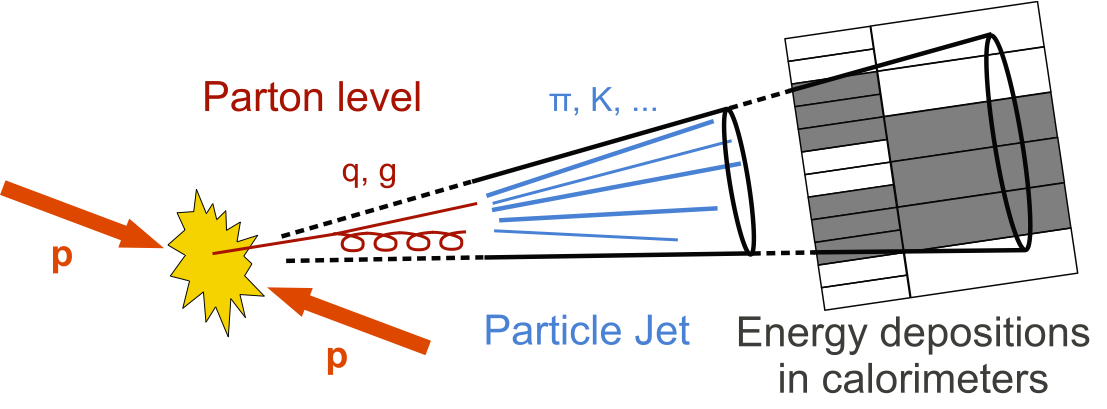
\includegraphics[width=13cm]{Chapter3/Sketch_Jet.png}
\caption{A pictorial representation of a jet.}
\label{fig:Jet}
\end{center}
\end{figure}
\vspace{-0.2in}

\subsubsection{Jet reconstruction}
The aim of jet reconstruction is to reconstruct and identify jets coming from the hadronization of partons.
This process can be divided into two parts: The first part reconstructs the individual jet constituents and the second part clusters
them together to produce a complete jet. 

For reconstruction of jet constituents, three different approaches are considered at CMS: a calorimeter based approach which utilizes the
information of the calorimeter energy deposits only; a Jet$-$Plus$-$Track (JPT) approach that improves
the calorimeter information by using the additional knowledge from the associated tracks; a Particle-Flow (PF) approach that attempts to combine the information
from all the relevant sub-detectors. A highly improved spatial and momentum resolution can be achieved by the use of PF approach
as compared to calorimeter or JPT approach. 

The jet clustering algorithms are used to cluster individual jet constituent particles to form a jet. These algorithms can be broadly divided into
two classes: the sequential recombination algorithms and the cone algorithms. The sequential algorithms work by combining a pair of particles based on the
closeness in some distance measure and then repeating the procedure for other particles until some stopping condition is reached. The main sequential algorithms
employed at CMS include, \kt~\cite{Catani:246812}, \antikt~\cite{Cacciari:2008gp} and Cambridge$/$Aachen (CA)~\cite{CMS-PAS-JME-09-001, Dokshitzer:1997in},
described by the distance measurements,
\begin{equation}
  \begin{split}
    & d_{ij} = \textrm{min}(k^{2p}_{\mathrm{T}i}, k^{2p}_{\mathrm{T}j}) \frac{\dR^{2}_{ij}}{R^{2}} \hspace{0.2in} \textrm{and}\\
    & d_{iB} = k^{2p}_{\mathrm{T}i},
  \end{split}   
\end{equation}
where, \\
$d_{ij}$: distance between $i$th and $j$th particle, \\
$d_{iB}$: distance of $i$th particle from the beam line, \\
$k_{\mathrm{T}}$: particle's transverse momentum, and \\
$\dR_{ij}$: spatial distance between $i$th and $j$th particles, $\sqrt{(\eta_{i} - \eta_{j})^{2} + (\phi_{i} - \phi_{j})^{2}}$. \\
The parameter $R$ determines the angular reach of a jet and is usually called the jet radius. The parameter, $p$ = 1 for \kt algorithm,
implies that this algorithm clusters the soft particles (low \pt) first, $p$ = $-1$ for \antikt algorithm
means that it clusters hard particles (high \pt) first and $p$ = 0 for CA algorithm performs an energy independent clustering. 
On the other hand, the cone algorithms define specific conical regions around the particles and put together all the particles inside the cone in the form of a jet 
such that the total momentum of the particles coincide with the cone axis. The famous cone algorithms include,
Iterative cone, Midpoint cone, SIScone etc. These algorithms mainly differ from each other in the strategy used to search for the stable conical region. 
The \fig{\ref{fig:JetClusterAlgo}} represents the behaviour of different jet clustering algorithms.
\begin{figure}[h]
\begin{center}
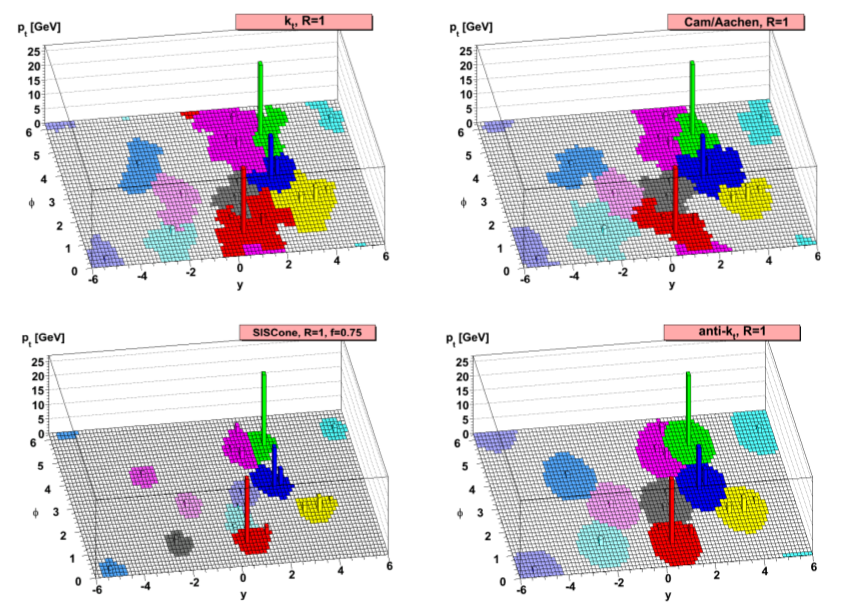
\includegraphics[width=13cm]{Chapter3/JetClusteringAlgo.png}
\caption{The behaviour of different jet clustering algorithms.}
\label{fig:JetClusterAlgo}
\end{center}
\end{figure}
%\vspace{-0.2in}

The sequential algorithms have a number of advantages over the cone algorithms, like: simplicity and detector independence, can be easily implemented in experimental
analyses and theoretical calculations, insensitive to hadronic effects, infrared and collinear safe\footnote{Infrared safety requires that the clustering
  algorithms should not be affected by the inclusion of an extra soft gluon and collinear safety requires that the jet clustering should remain same for
  splitting of a parton into two partons. Both of these lead to finite perturbative calculations upto any order.} etc.
The analysis in this thesis considers the particle flow jets clustered using the \antikt algorithm. A detailed description of these has been provided below:

\noindent
\underline{\bf{Particle flow reconstruction algorithm}}:
The particle flow algorithm of CMS~\cite{Sirunyan:2017ulk, CMS-PAS-PFT-09-001} relies mainly on the high efficiency of track reconstruction and fine granularity
of ECAL and HCAL. This algorithm works by linking the energy clusters in the calorimeters with the tracker signals to create a complete picture of the event.
Since, this algorithm reconstructs individual particles corresponding to each sub-detector first, a dedicated calibration can be done and the impact of
non-compensating nature of HCAL can be mitigated to get an overall good response. Also due to the availability of tracking and vertex information,
the impact of pile-up collisions can be reduced. The list of individual particles from each sub-detector is then used to reconstruct jets, \met, $\tau$, b-jets etc. 

This algorithm is performed in three main steps. The first step builds the basic elements of PF algorithm, like the
reconstruction of charged particles tracks in the tracker and energy clusters in the
calorimeters. The energy clustering in HCAL starts by searching for a seed channel, a local energy maxima. The topological clusters are then formed by adding neighbouring
channels to it. The energy of each calorimeter channel is required to be above some predefined threshold, in order to avoid any contributions from electronic noise etc.
The energies and positions of the final clusters are determined using an iterative method by re-weighting the contributions of individual channels
on the basis of their distance from the seed channel. 
This step is then followed by a second step that involves the building of PF blocks using a mechanism known as link algorithm, which performs the
linking of the tracks with the energy deposits in ECAL and HCAL, compatible with the electromagnetic and hadronic shower profiles.
A link between ECAL and HCAL energy deposits is also made if the ECAL cluster position lies within the envelope of HCAL cluster. The tracks are also linked to
the muon hits in the muon system, thereby forming global muons. The resultant PF block consists of a maximum of three elements.
The quality of these blocks is determined by the compatibility of its elements, either in the form of $\eta-\phi$ distance in case of track$-$to$-$cluster and
cluster$-$to$-$cluster links or in the form of $\chi^{2}$ fit in case of track$-$to$-$muon links. The third step consists of the reconstruction of final PF objects on the
basis of the PF blocks.

The performance of PF algorithm has been studied using simulated events~\cite{CMS-PAS-PFT-09-001}. A great precision is achieved, using tracker and ECAL,
for the measurement of around 90$\%$ of jet energy taken by the charged hadrons and photons.
The remaining 10$\%$ of jet energy shared by neutral hadrons is measured solely in HCAL and 
has an energy resolution of 120$\%/\sqrt{E}$.

\noindent
\underline{\bf{\boldmath{$\Antikt$} clustering algorithm}}:
The default jet clustering algorithm used in CMS is one of the sequential recombination algorithm, the \antikt~\cite{Cacciari:2008gp} algorithm.  
It determines two distance measures for a pair of particles ($i,j$) as
\begin{equation}
  \begin{split}
    & d_{ij} = \textrm{min}(k^{-2}_{\mathrm{T}i}, k^{-2}_{\mathrm{T}j}) \frac{\dR^{2}_{ij}}{R^{2}} \hspace{0.2in} \textrm{and}\\
    & d_{iB} = k^{-2}_{\mathrm{T}i}.
  \end{split}   
\end{equation}
This algorithm works by finding the distance of $i$th particle from the closest $j$th particle ($d_{ij}$) and from the beam line ($d_{iB}$), by using
the definition of distance measures given above. If $i$th particle is closer to $j$th particle as compared to beam line ($d_{ij}$ is smallest),
it replaces $i$th and $j$th
particle with a single new particle of momentum $k_{\mathrm{T}i}+k_{\mathrm{T}j}$, often called a pseudojet, as it is neither a single particle nor a full jet.
However, if the $i$th particle is closer to beam line as compared to $j$th particle ($d_{iB}$ is smallest), then it removes the $i$th particle from the
list of particles under study and considers $i$th particle as an inclusive jet. The
algorithm then repeats this procedure with a new pair of closest particles$/$pseudojets, until it includes all the particles. The CMS uses \antikt algorithm
corresponding to two values of jet radius, viz 0.4 and 0.8, forming AK4 and AK8 jets.
\subsubsection{Jet energy corrections}\label{Se:JetEnCorr}
The energy of a reconstructed jet is not the same as that of the true energy of a particle level jet. The primary reason being the non-linearity and non-uniform
response of calorimeters, especially HCAL.    
The jet energy corrections (JEC)~\cite{CMS-PAS-JME-07-002} are a set of tools that performs the mapping of the reconstructed jet energy to the actual particle-level energy.
At CMS, a multi level factorized approach to JEC has been considered where each level correspond to a different correction of specific type. These corrections
are extracted using the data-driven as well as the simulation methods and are provided as $\textit{in-situ}$ calibrations in data and MC.  
Each correction level is dependent on various jet quantities and provides a scaling to the jet four momentum\footnote{($p_{x}, p_{y}, p_{z}, E$)}.
These corrections are always applied sequentially in a fixed order. The different JEC levels are represented in \fig{\ref{fig:JEC_levels}} and are described below:
\begin{figure}[h]
\begin{center}
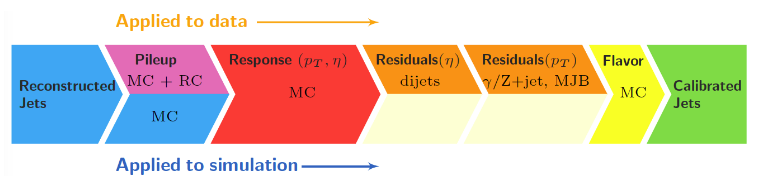
\includegraphics[width=15cm]{Chapter3/JES_diagram.png}
\caption{Different jet energy correction levels applied to data and MC.}
\label{fig:JEC_levels}
\end{center}
\end{figure}
\vspace{-0.4in}
\begin{itemize}[leftmargin=*]
\item {\bf{L1 Offset}}: The purpose of the L1 correction is to subtract any energy contribution coming from the pile-up and underlying events~\cite{Cacciari:2007fd}.
  This correction, in principle, removes the dependence of data sample on the luminosity, so that the further corrections are applied on a
  luminosity independent sample. These corrections are estimated using the events processed with and without considering pile-up overlay in a simulated
  sample of QCD dijet and parameterized as a function of energy density $\rho$, jet area, $\eta^{\textrm{jet}}$ and $\pt^{\textrm{jet}}$. The residual differences between
  data and simulation are corrected as a function of $\eta$ using a random cone method implemented using zero-bias events, resulting into different L1 corrections for
  data and MC.
\item {\bf{L2 Relative}}: These corrections are applied to both data and MC to make the jet response uniform as a function of pseudorapidity, $\eta$.
\item {\bf{L3 Absolute}}: After correcting the jet response in $\eta$, it is also made uniform in $\pt$ using L3 corrections. The L2 and L3 corrections are now
  computed together using QCD dijet samples and are collectively called L2L3 MC-truth corrections.
\item {\bf{L2L3 Residual}}: This correction is determined by the $\textit{in-situ}$ measurements of absolute and relative jet energy scales and is meant to
  correct the small differences between data and MC, of the order of a few $\%$, in jet response. A correction factor, equivalent to the residual difference
  between data and MC, is applied only to data. 
\end{itemize}
Apart from these, an optional L5 flavor correction derived using Z$+$jet and $\gamma+$jet simulated samples, is also applied in some cases. The analysis in this thesis
considers the essential L1, L2, L3 and L2L3 corrections only. Each correction level also has the related uncertainties, forming the biggest source of systematic error
in a jet measurement. 
\subsubsection{b-tagging of a jet}\label{Se:Jet_btagging}
The jets arising from the hadronization of b-quarks are known as b-jets. The b-jets have many distinctive signatures (\fig{\ref{fig:bjet}}) like,
long lifetime ($\sim$ $10^{-12}$\unit{s}),
large mass (4.2\unit{GeV}), high track multiplicity ($\sim$ 4$-$5), relatively large semi-leptonic branching ratio ($\sim$ 20$\%$ for each of $e^{-}$ and $\mu^{-}$), hard
fragmentation function\footnote{A significant fraction of initial b-quark's momentum is taken away by b-hadrons.} etc., which leads to their precise
measurement. The CMS with its rigorous charged particle tracking, powerful lepton identification and highly segmented calorimetry, is well matched for the task
of b-jet identification~\cite{Chatrchyan:2012jua, Sirunyan:2017ezt}. The b-tagging is a kind of reconstruction procedure that utilizes 
various b-hadron properties and based on these, assigns a ``likelihood'' to each jet, of the presence of b-hadrons.
\begin{figure}[h]
\begin{center}
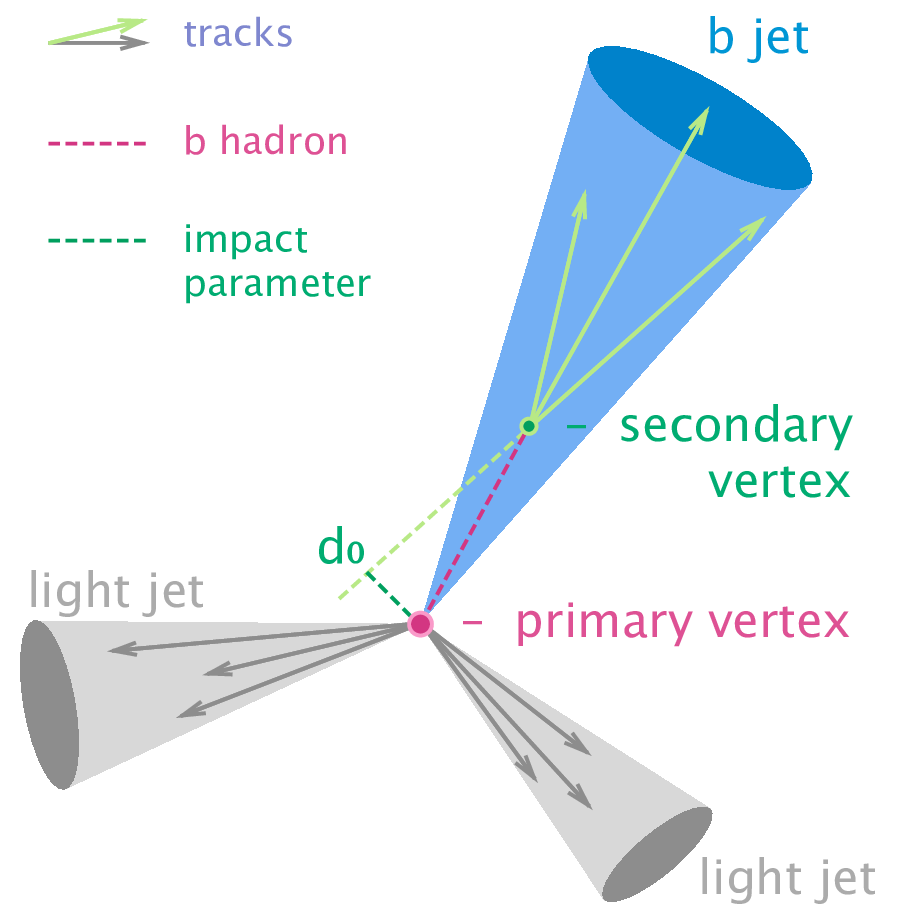
\includegraphics[width=5cm]{Chapter3/bjet.png}
\caption{A depiction of a b-jet emerging from the primary vertex.}
\label{fig:bjet}
\end{center}
\end{figure}


\begin{figure}[h]
\begin{center}
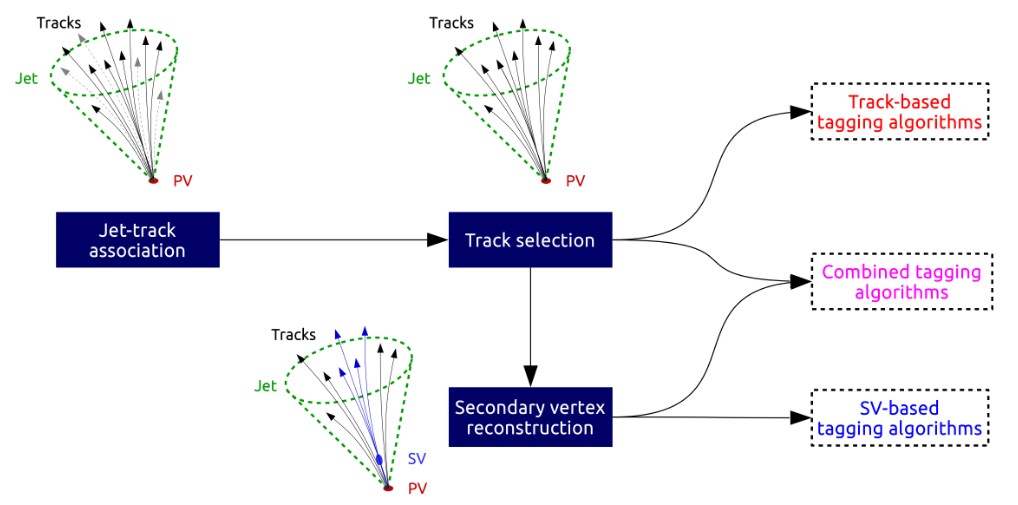
\includegraphics[width=15cm]{Chapter3/btagAlgorithms.png}
\caption{An illustration of b-tagging algorithms.}
\label{fig:bjetAlgo}
\end{center}
\end{figure}

A number of b-tagging algorithms have been deployed at CMS that mainly differs in their complexity and input information. All these algorithms provide a numerical
discriminator for a jet in the output whose value determines the b-tagging status of the jet. The higher is the value of discriminator, the larger is the probability of
the jet being a b-jet. These b-tagging algorithms are constructed on the basis of the information gathered from either the tracks or secondary vertex or soft lepton or
any combination of these, as presented in \fig{\ref{fig:bjetAlgo}}.
The main b-tagging algorithms employed in CMS are:
%\vspace{-0.1in}
\begin{itemize}[leftmargin=*]
\item {\bf{Track Counting (TC) algorithm}}: This approach exploits the long lifetime of b-hadrons and considers the charged tracks associated with it.
  It computes the significance of the signed impact parameter\footnote{Impact Parameter (IP) is defined as the minimum distance between the track and primary vertex, the
    sign of IP is determined by the scalar product of IP segment with the jet direction.} of all the good tracks, arrange them in decreasing significance and assign the
  significance of $N$th track to the discriminator. It leads to an algorithm of high efficiency for $N$ = 2 and high purity for $N$ = 3. 
\item {\bf{Jet Probability (JP) algorithm}}: This algorithm uses information from all selected tracks in a jet. Using a sample of tracks with
  negative impact parameters, it builds a probability distribution
  function (PDF) that considers the probability of a track to be originating from the primary vertex. Based on this PDF, a probability pointer is assigned to each
  track and a discriminator is built using full set of tracks. A version of JP algorithm, known as jet B probability is also used that considers only the four
  highest displaced tracks matching with the reconstructed multiplicity of the b-hadron decay vertex. 
\item {\bf{Soft Lepton (SL) algorithm}}: This algorithm identifies the b-hadrons on the basis of their semi-leptonic decays as the leptons from b-decay usually tend
  to have high \pt relative to the jet axis. The corresponding b-tag discriminator is the result of the neural network\footnote{A neural network
    is a hardware$/$software system designed on the basis of working of neurons in the human brain.} build up using lepton \pt, impact parameters
  and some other variables.
\item {\bf{Simple Secondary Vertex (SSV) algorithm}}: This algorithm considers the reconstruction of secondary vertex from the b-hadron decay using an adaptive
  vertex finder technique and uses the variables associated with it to compute the discriminator value.
\item {\bf{Combined Secondary Vertex (CSV) algorithm}}: This is the most sophisticated and complex approach making use of all the known information like
  secondary vertices, lifetime, IP significances, decay lengths etc. This algorithm has the capability to provide a discrimination even when no secondary vertex is
  reconstructed. It uses a list of variables and feeds them as input into a likelihood ratio which is then used to compute the discriminator value.
  A ``version 2'' of this algorithm known as ``CSVv2'' has
  also been introduced during LHC Run II that makes use of the artificial neutral networks instead of likelihood ratio.   
\end{itemize}
\vspace{-0.2in}
These algorithms have a b-tag identification efficiency varying in a range of $40-70\%$. These are available in three working points:
loose, medium and tight, corresponding to light flavour mis-tagging rate of 10$\%$, 1$\%$ and 0.1$\%$, respectively.
At CMS, these algorithms are determined using the inclusive multijet, muon enriched jets and dilepton $t\bar{t}$ data samples,
the jets are required to be PF jets clustered using \antikt algorithm having a \pt $>$ 20\unit{GeV} and lying within the tracker acceptance region, $|\eta|$ $<$ 2.4. 
\subsubsection{Jet identification}\label{Se:JetID}
The reconstructed and calibrated jets contain a significant fraction of fake jets coming mainly from the electronic noise and other detector artifacts.
In order to identify and locate a good collection of jets to be used in an analysis, a set of identification variables are defined~\cite{Web:JetId}, listed as below:
\vspace{-0.1in}
\begin{itemize}[leftmargin=*]
  \setlength\itemsep{0.1em}
\item {\bf{Charged hadron fraction}}: The fraction of energy deposited in HCAL by charged hadrons.
\item {\bf{Neutral hadron fraction}}: The fraction of energy deposited in HCAL by neutral hadrons.
\item {\bf{Charged electromagnetic fraction}}: The fraction of energy deposited in ECAL by charged constituents of the jet.
\item {\bf{Neutral electromagnetic fraction}}: The fraction of energy deposited in ECAL by neutral constituents of the jet.
\item {\bf{Number of constituents}}: The number of particles in a jet.
\item {\bf{Charged multiplicity}}: The number of charged particles in a jet.
\end{itemize}
\vspace{-0.1in}
\section{Event Simulation}
Event simulation is an integral part of any high energy physics experiment right from the designing stage to the final analysis.
It is almost impossible to perform a physics analysis without the use of simulated data. It acts as a reference to the detector output as well as
allows us to study the behaviour and consequences of any new theory without having observed it directly. 
The various efficiencies and correction factors used by the analyses are computed by comparing experimental and simulated data while a number of
systematic uncertainties are computed using simulated data alone. In general, the quality of any physics result is strongly
influenced by the quality of simulation involved. 

Event simulation produces events that perfectly mimic the output from an actual detector. The various steps involved in a simulation chain are presented schematically
in \fig{\ref{fig:SimChain}}. 
\begin{figure}[h]
\begin{center}
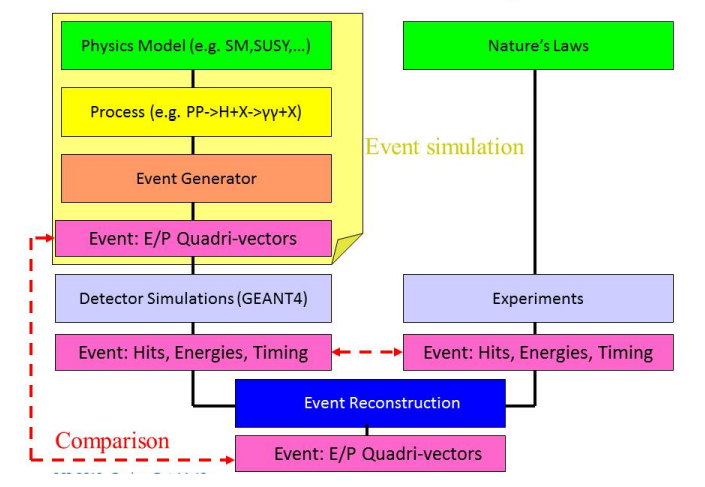
\includegraphics[width=15cm]{Chapter3/SimulationChain.png}
\caption{Event simulation and data analysis chain.}
\label{fig:SimChain}
\end{center}
\end{figure}
%\vspace{-0.2in}

As the first step of the simulation chain, the ``Physics Model'' in which the calculation has to be performed, is selected. The physics model can be the
standard model (to simulate background processes) or any model beyond the standard model (to simulate signal processes of new physics).  
The simulation process is defined at the next level by specifying the input$/$output particles and the order of calculation. The expressions for matrix element and
probability cross-section are prepared automatically on the basis of the selected physics model.   
At the ``Event Generator'' level, the matrix element is integrated over the entire phase space and the random samples of all final state particles, along with
the information of their energy-momentum, are generated. The generated events are then made to propagate through a ``Detector Simulation'' model
that represents the simulation of an actual detector.    
The huge amount of information produced in output by the detector simulation exactly replicate the output from a real detector. At this level,
both the theoretical simulated data and experimental detector data are at equal footing and can be compared with each other. The simulated data
is reconstructed using the same reconstruction programme as used for real data. Comparison of reconstructed simulated data with real data
provides a test of self-consistency of the underlying physics model, though any discrepancy between the two may hint towards some new physics. 
The final analysis is performed using a data analysis toolkit, known as ROOT~\cite{Brun:1997pa}. The simulated and observed events passing various
filters and cuts are studied and compared by organizing them in the form of histograms. At CERN, the simulation and analysis of data is performed using
a data distribution grid system known as WLCG (Worldwide LHC Computing Grid)~\cite{WLCG}. This infrastructure is based on the tiers
computing centers, distributed all around the world.

The two main components of event simulation process, viz, event generation and detector simulation are described in more detail in the sections below.
\subsection{Event generation}
Event generation~\cite{Buckley:2011ms, Dobbs:2004qw} is the first stage of the simulation process.
It is based on software programs that use Monte Carlo (MC) methods~\cite{robert2004monte, MC_Tech} to simulate events.
A Monte Carlo technique is basically an integration tool based on random sampling\footnote{A method of selecting a sample from a large statistical population such that
  each sample in the population has some predefined probability of being selected.}. It is mainly used to obtain approximate numerical solutions
of the analytical problems which are otherwise too complicated to solve. 

The main objective of event generators is to accurately provide the description of an actual particle collision.
In a high energy pp collision, the formation of a single event involve several steps as depicted in \fig{\ref{fig:EvtGen}}. At the start, the two partons
are selected, in flavor as well as in color, from each of the two colliding protons. These partons are allowed to radiate gluons, known as initial state radiation,
before interacting. The hard scattering process occurs upon interaction and results into the production of two or more final state particles, probably via a
resonance state. These final state particles can further decay into other particles producing
several daughters. The remaining quarks and gluons undergo the emission of parton showers before the final hadronization stage occurs, resulting into the
recombination of partons to form hadrons. In addition to these, the left over partons (known as beam remnants) of a proton,
after the parton underwent hard scattering is pulled off, can interact with each other, leading to the multiple parton interactions (MPI).
These MPIs result into creation of multiple vertices as well as addition of extra tracks and energy deposits interfering with the main collision,
referred to as the underlying events (UE). 
\begin{figure}[h]
\begin{center}
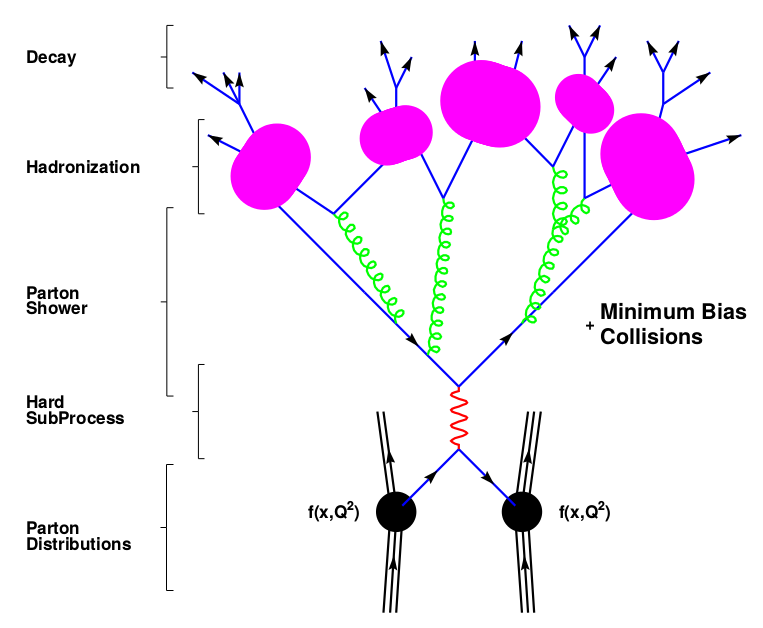
\includegraphics[width=13cm]{Chapter3/EventGeneration.png}
\caption{Sequential steps involved in the formation of an event.}
\label{fig:EvtGen}
\end{center}
\end{figure}
%\vspace{-0.2in}

The event generators also formulate an event in the same sequence through the use of different theoretical models for different physics aspects, like
hard and soft interactions, initial$/$final state parton showers, parton distribution functions, multiple interactions, underlying events,
parton hadronization and decay etc. Simulating these aspects of a process require the calculation of relevant matrix element involving loop
diagrams up to many orders, achieved by the use of dedicated MC techniques.

The cross-sections for various processes are stored within the event generators which are solved by the use of MC integration techniques.
The cross-section of a $2\rightarrow2$ process at tree-level is given by,
\begin{equation}
\sigma(ab\rightarrow{cd})=\sum_{ab}\int_{0}^{1}\int_{0}^{1} \hat{\sigma}_{ab\rightarrow{cd}}
            \left(\hat{s},\alpha_{s}(\mu_{R}^{2}),\frac{Q^{2}}{\mu_{F}^{2}},\frac{Q^{2}}{\mu_{R}^{2}}\right)f_{a}(x_{1},\mu_{F}^{2})f_{b}(x_{2},\mu_{F}^{2})dx_{1}dx_{2} 
\label{eq:gamJetXS}
\end{equation}
Here $Q$ is the scale of hard interaction while $\mu_{F}$ and $\mu_{R}$ are factorization and renormalization scale. 
The quantity, $\hat{s}=x_{1}x_{2}s$, $s$ is the center-of-mass energy of collision, $x_{1}$ and $x_{2}$ are the fractions of total proton's momentum, carried by two
interacting partons. The functions $f_{a}(x_{1},\mu^{2}_{F})$ and $f_{b}(x_{2},\mu_{F}^{2})$ are the probability density function for two partons,
also known as parton distribution function (PDF)~\cite{Martin:2009iq},
representing the probability of carrying a momentum fraction $x_{1}$ and $x_{2}$ by parton $a$ and $b$ respectively.
The initial partons for a hard interaction are selected by the use of PDF.
These PDF's are determined experimentally from deep inelastic scattering processes, Drell-Yan processes, and jet production at high energies.
The $\hat{\sigma}$ is the parton level cross-section of the sub-process $ab\rightarrow{cd}$.
The expression is integrated using MC techniques over the entire phase space.
If the expression contains loop corrections, then integration over loop propagators is also performed. The multi-dimensional integration
yield the total cross-section of the process. The event after passing through the various event generation levels is then
passed to the detector simulation stage.
\subsubsection{MC event generators}
A number of event generators based on MC techniques are used in present day colliders. These can be divided into general-purpose generators and specific generators.
The specific generators are good for simulating any particular physics aspect but need to be interfaced with general-purpose generators to simulate a complete
event. Examples of some of the general-purpose generators are: \pythia~\cite{Sjostrand:2014zea}, \madgraph~\cite{Alwall:2014hca},
$\herwigpp$~\cite{Bahr:2008pv}, \alpgen~\cite{Mangano:2002ea} and \sherpa~\cite{Gleisberg:2008ta}. The analysis
documented in this thesis uses \pythia and \madgraph as the generators to simulate various signal and background processes. A brief description of these
are given below.
\paragraph{\pythia}
\hspace{\parindent} It is one of the oldest general-purpose event generator used for lepton as well as hadron colliders.
Its hadronization model is based on the Lund string model~\cite{Sjostrand:1986hx},
consisting of around 240 hard scattering processes. It is a leading order (LO) event generator and
considers only two particles in initial and final states. It consists of models for initial and final state parton showers, hard processes matching and
merging, multi parton interactions, underlying events etc. It also has the facility to interface with external programs. 
\paragraph{\madgraph}
\hspace{\parindent} \pythia is an ideal event generator for simulating $2\rightarrow{2}$ processes, but in actual collisions, most of the processes contain
more than two particles in final state. The \madgraph~\cite{Alwall:2014hca} matrix element generator has the capacity to produce the processes with up to
nine particles in the final state. It uses ALOHA package~\cite{deAquino:2011ub} to automatically generate the amplitudes of relevant sub-processes.
The events simulated using \madgraph are put in some standard event format files known as Les Houches format files (LHE files)~\cite{Alwall:2006yp} which
are then passed to \pythia to simulate parton showering and hadronization. The \pythia also performs matching and merging of the matrix elements (ME)
with the partons showers (PS) using CKKW algorithm~\cite{Krauss:2002up} and MLM scheme~\cite{Mangano:2001xp}.
\subsection{Detector simulation}
In order to simulate the behaviour of particles within the detector, a software based model representing a virtual detector has been used.
The event generator output is made to pass through this detector simulation model to obtain a replica of actual collision data.
With increase in complexity and resolution of the detectors, the detailed simulation of an experimental setup has become a challenging task. It
requires efficient and sophisticated tools to accurately reproduce the behaviour of detector in the presence of collision particles.

In CMS, the simulation of the detector is performed using an object oriented toolkit known as \geant~\cite{Agostinelli:2002hh}.
The \geant consists of a set of C$++$ libraries
which can be used to simulate any detector system. It simulates the particle interactions in matter on the basis of Monte Carlo methods. 
The \geant package provide accurate description of various detector aspects like, detector geometry, material of different detector components and the
dead material such as bolts, cables, support etc. It consists of a set of physics models that are able to handle the various particle's interactions with
the matter over a wide range of energy, ranging from few hundred $\unit{eV}$s to \unit{TeV}. Starting from the event generator output, the events are made
to propagate through the detector simulation while taking into account the magnetic field for charged particles as well as the various interactions of
particles with matter like bremsstrahlung, multiple scattering, photon conversions, scintillation, ionization, cherenkov light etc.
Finally, the raw output similar to that of the actual detector data is obtained. 


\clearemptydoublepage
\chapter{Search for light and heavy flavor excited quarks}
This chapter documents in great detail the various steps and procedures followed in the analysis of CMS data to search for any signature of excited light and
heavy quark presence in \gamjet and \gambjet final states respectively. 
\section{Analysis strategy}
In high energy physics, the invariant mass is a very important parameter to determine the nature of a process. It is a Lorentz invariant
quantity and is defined as the system mass constructed using the Lorentz invariant energy and momentum. For a single particle, the invariant mass
is equivalent to its rest mass, given by $m^{2}$ = $E^{2} - p^{2}$, in natural units\footnote{In natural units, $\hbar$ = $c$ = 1}. This relation is also true for a
system of masses with $E$ and $p$ representing the total energy and momentum of the system. In a process that occurs through a resonance,
the invariant mass of final state particles is equivalent to the rest mass of the resonance. The process has a larger cross-section corresponding to the energy of
resonance mass. 

If we plot the invariant mass distribution of final state particles for a large sample of events, the number of events
corresponding to the resonance mass will be relatively larger as compared to the neighbouring masses. %\footnote{$N$ = $\sigma \times L$,
%  $N$ = number of events, $\sigma$ = cross-section and $L$ = luminosity}.
The resonance will appear as a peak over the continuous distribution, arising due to
the standard model processes referred to as the background processes, with the peak-width proportional to the resonance's life time.
The background due to various SM processes is subtracted either by the use of Monte Carlo simulated background samples or by the use of data driven
technique where the background is evaluated by fitting the invariant mass distribution with a smooth parameterization. Any significant deviation from
the smooth distribution at any point in data is considered as a signal of new physics. In case of absence of any significant deviation, the resonance signal model,
simulated on the basis of the underlying theory, is used to evaluate a signal cross-section (mass), above (below) which the presence of the signal
is discarded with some statistical significance.

\subsection{Excited quark analysis}
In this analysis, the resonance signals considered are the excited states of light $q$ = $u,d$ and heavy $b$ quarks. The underlying processes are
pp $\rightarrow$ \qstar $\rightarrow$ \gamjet and pp $\rightarrow$ \bstar $\rightarrow$ \gambjet. The invariant mass distribution spectra of \gamjet and \gambjet
are the most important distributions for this study, which have been analyzed to investigate the presence or absence of excited quark signals.
A detailed overview of the signals and backgrounds of this study is presented in sections below.
\subsubsection{Signals}
This analysis considers the \qstar and \bstar signals decaying into \gamjet and \gambjet final states respectively,
where the jet can be a light quark, a gluon or a b-quark.
The Feynman diagrams representing the various physics processes contributing to this channel are presented in \fig{\ref{fig:qstarSig}}.
Among these, the most dominant quark-gluon
fusion process has been considered for this analysis. This process contributes through two Feynman diagrams in s- and t-channel as shown in \fig{\ref{fig:qgFusion_s_t}}.

%\vspace{-0.2in}
\begin{figure}[h]
\begin{center}
\subfloat[s-channel]{\label{fig:qgFusion}\includegraphics[width=5cm]{Chapter4/Feynman_diagrams/Signal_qgFusion.pdf}}
\hspace{0.1 in}
\subfloat[t-channel]{\label{fig:qqbarAnni}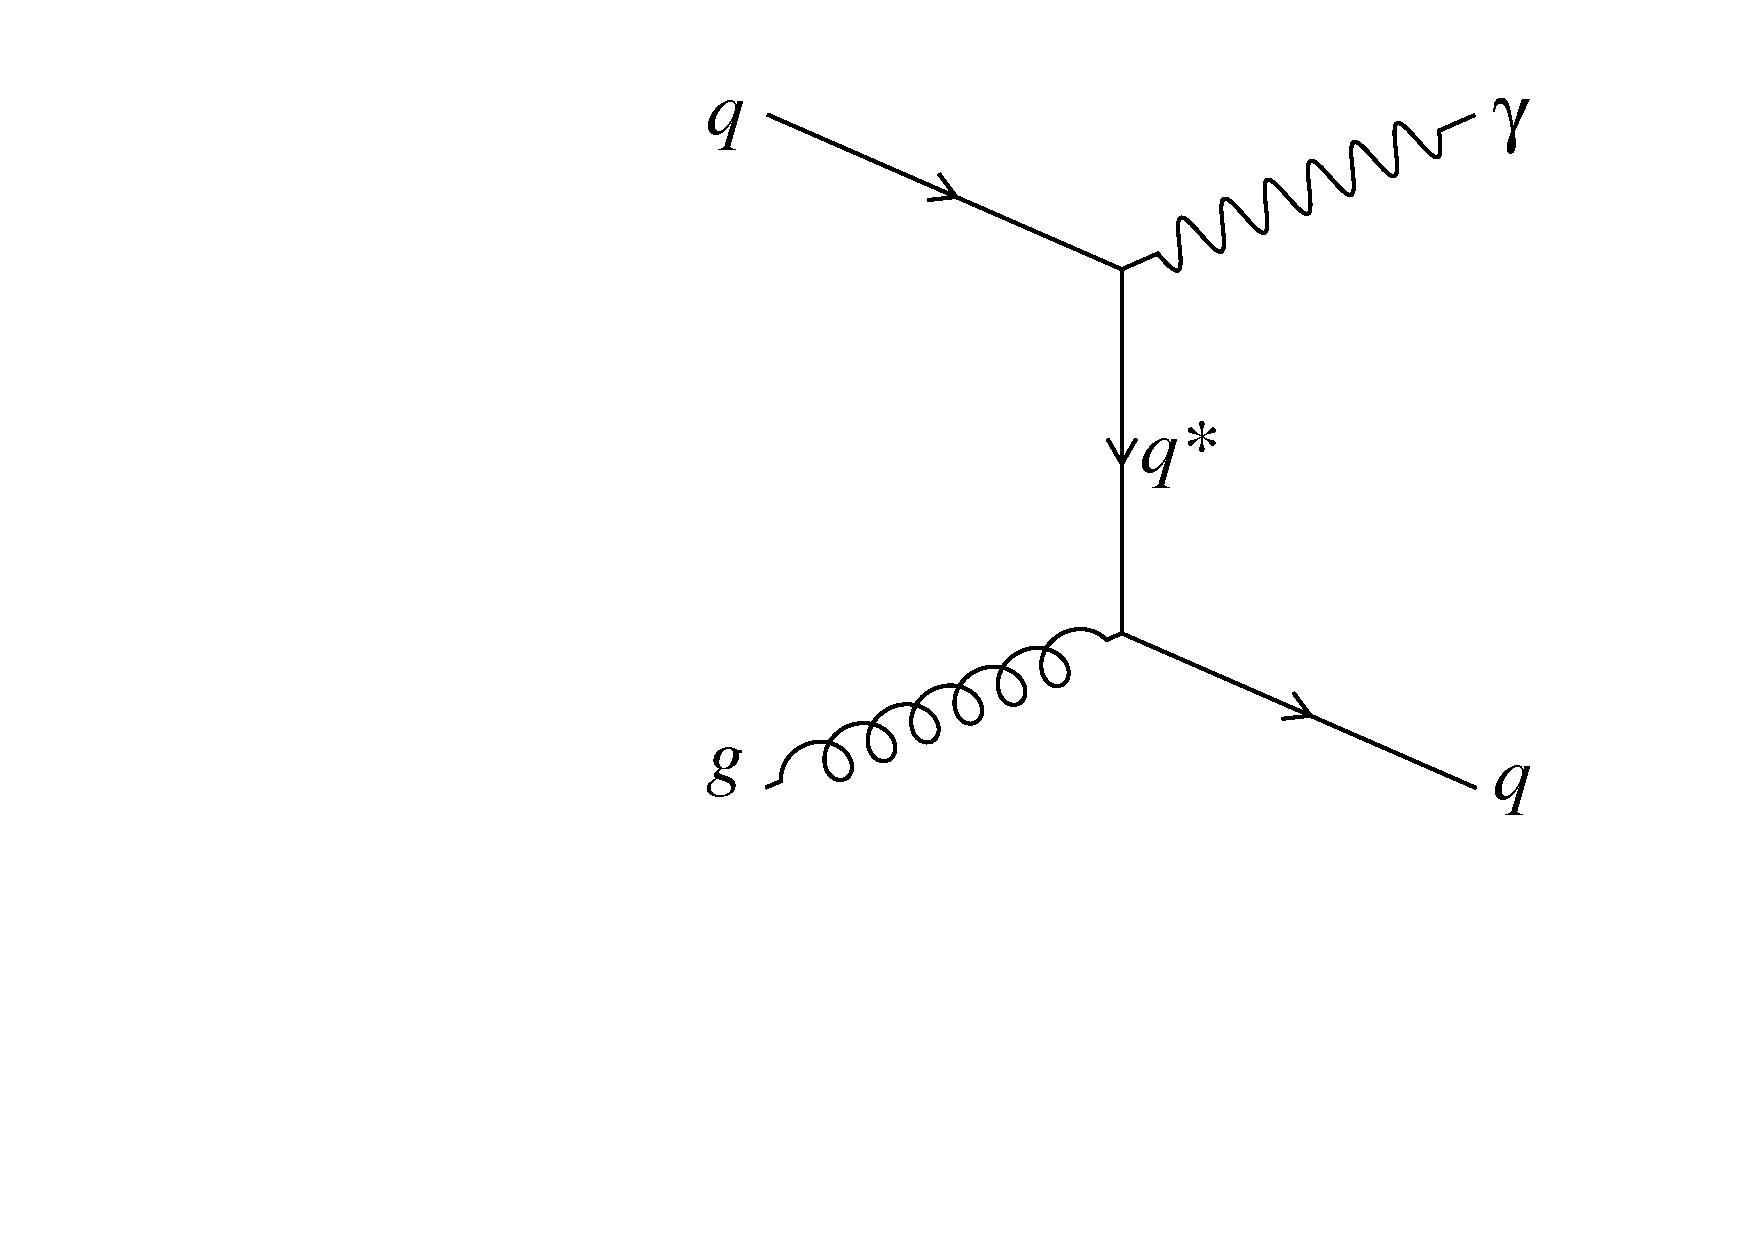
\includegraphics[width=5cm]{Chapter4/Feynman_diagrams/Signal_qgFusion_t.pdf}}
\hspace{0.1 in}
\caption{Feynman diagrams for quark-gluon fusion process in s and t channel.}
\label{fig:qgFusion_s_t}
\end{center}
\end{figure}
%\vspace{-0.2in}

The resonance will show its presence in the form of a bump in the s-channel and in the form of an excess of events in t-channel,
over the continuum invariant mass distribution of $\gamjet$.
\subsubsection{Backgrounds}
In pp collisions, the $\gamjet$ channel has a rather clean and simple signature within the detector. Still, many known SM processes can mimic this final state and
form the backgrounds of this study. These potential physics backgrounds are reported below as per their dominance:
\paragraph {\bf{SM $\gamjet$}}
\hspace{\parindent} The SM $\gamjet$ processes where a photon and a jet are produced in the hard collision, form the most dominant and irreducible
background for this study. A number of processes including quark-gluon compton scattering (qg $\rightarrow$ q$\gamma$), quark-antiquark annihilation (q$\bar{\textrm{q}}$
$\rightarrow$ g$\gamma$) and gluon-gluon fusion (gg $\rightarrow$ g$\gamma$) contribute to this background. The Feynman diagrams
representing these processes are shown in \fig{\ref{fig:GJ_Bkg}}. The qg scattering process dominates the total SM $\gamjet$ cross-section over the entire \pt range.
The contribution from the q$\bar{\textrm{q}}$ annihilation process is lesser, though it increases with increasing $\pt$. The gg fusion process, being a NLO process,
contributes negligibly. 

\vspace{-0.2in}
\begin{figure}[h!]
\centering
\subfloat[qg compton scattering]{\label{fig:qstarGJa}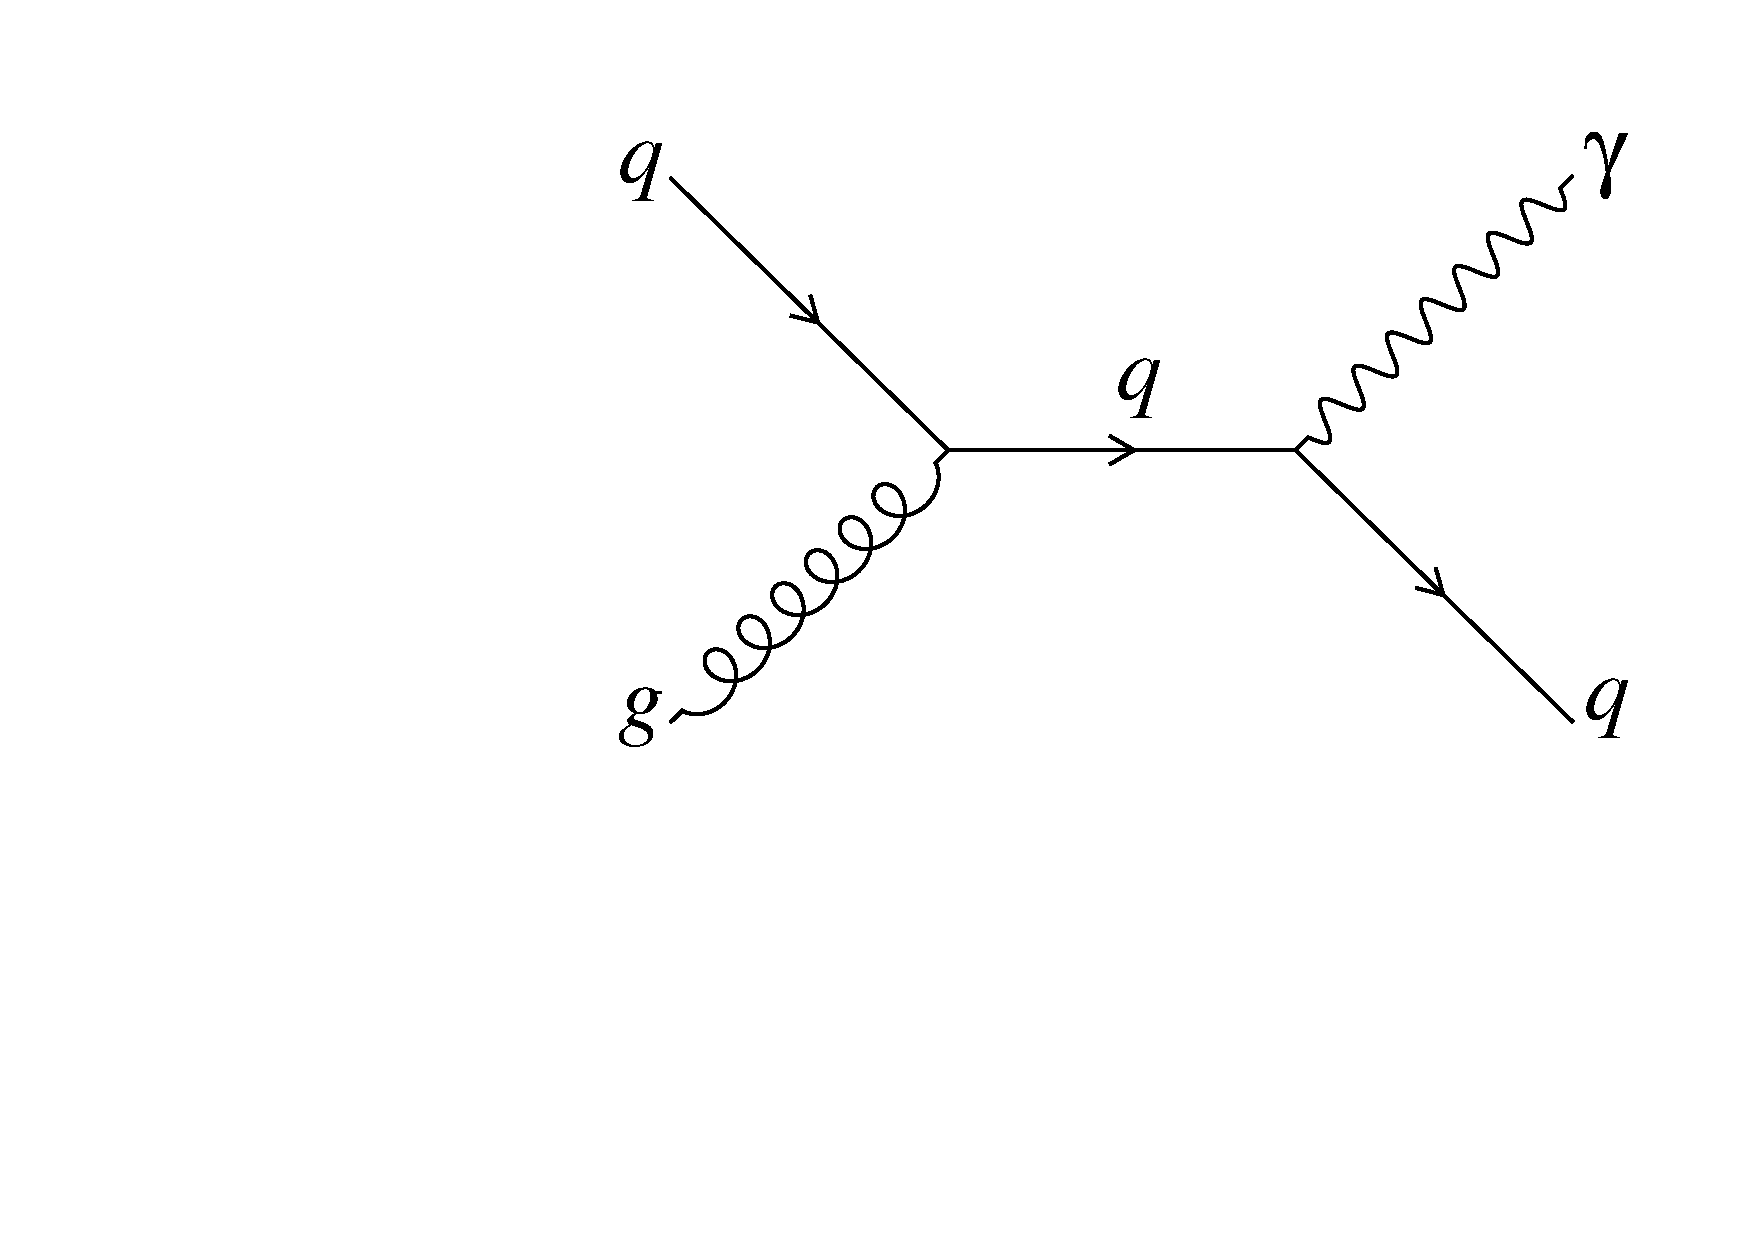
\includegraphics[width=4.4cm]{Chapter4/Feynman_diagrams/SMBkg_qgscattering.pdf}}
 \hspace{0.5cm}
 \subfloat[q$\bar{q}$ annihilation]{\label{fig:qstarGJb}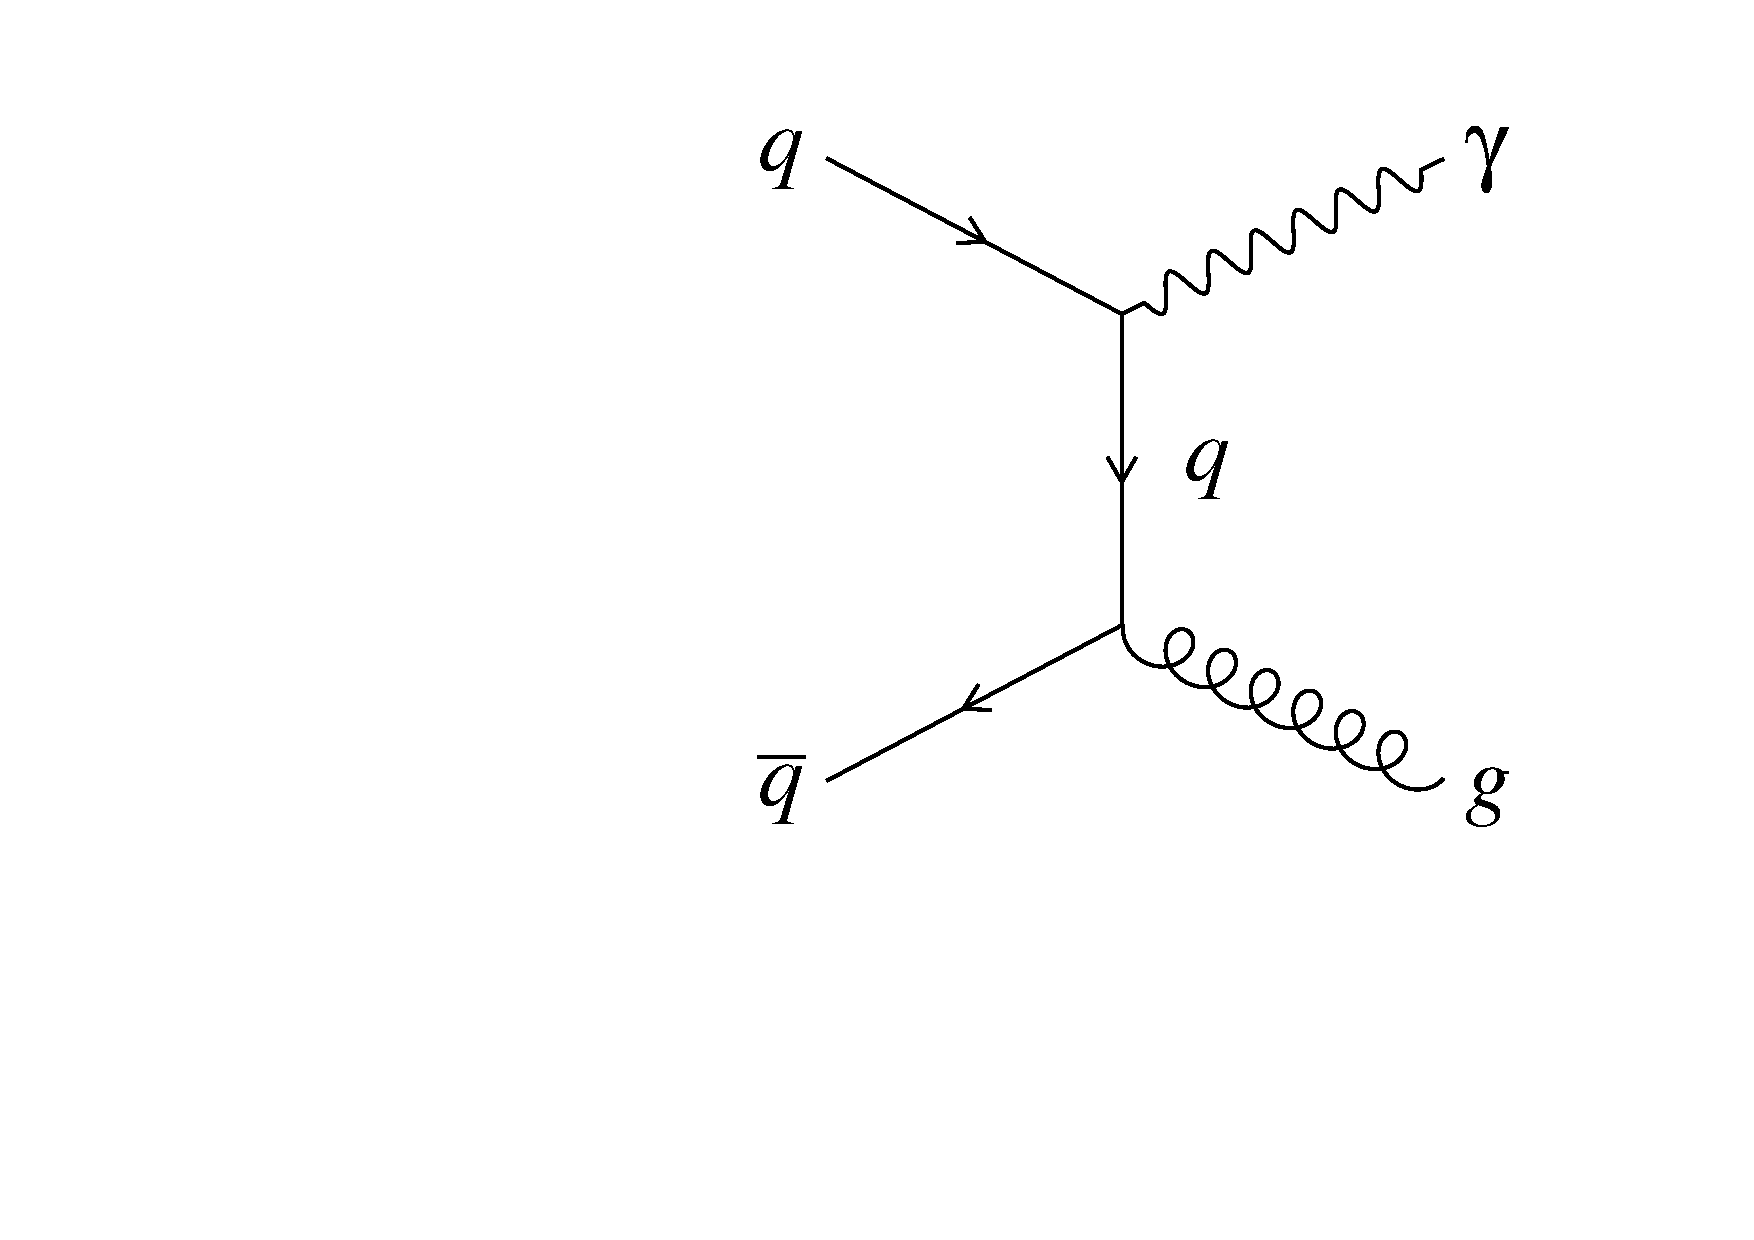
\includegraphics[width=4.4cm]{Chapter4/Feynman_diagrams/SMBkg_qqbarAnni.pdf}}
 \hspace{0.5cm}
 \subfloat[gg fusion]{\label{fig:qstarGJc}\includegraphics[width=4.4cm]{Chapter4/Feynman_diagrams/SMBkg_ggfusion.pdf}}
 \caption{Standard model background contribution from $\gamjet$ processes.}
\label{fig:GJ_Bkg}
\end{figure}
\paragraph {\bf{QCD dijet}}
\hspace{\parindent} The SM dijet processes where two jets are produced in the hard scattering, can form a background to a $\gamjet$ process if one of the jets fragments
into a highly energetic $\pi^{0}$ which then decays into a pair of overlapping photons and gets reconstructed as a single photon in the detector.
A number of processes like the ones shown in \fig{\ref{fig:QCDDijet_bkg}}, contribute to this background.
The production cross-section of these processes is around 10$^{4}$ times larger than the SM $\gamjet$ processes. But, since the probability of a jet faking a photon
is about $10^{-4} - 10^{-3}$, this background form the second largest background of this study. Also, the cross-section for these processes falls very swiftly
($\sim$ $\pt^{-4}$) with increasing $\pt$, so this background has significantly lower contribution at high $\pt$.

\begin{figure}[h!]
\centering
 \includegraphics[width=4.4cm]{Chapter4/Feynman_diagrams/QCDBkg_gqTogq.pdf}
 \includegraphics[width=4.4cm]{Chapter4/Feynman_diagrams/QCDBkg_ggTogg_T.pdf}\\
 \includegraphics[width=4.4cm]{Chapter4/Feynman_diagrams/QCDBkg_ggToqqbar_S.pdf}
 \includegraphics[width=4.4cm]{Chapter4/Feynman_diagrams/QCDBkg_qqbarToqqbar_S.pdf} 
 \caption{Standard model background contribution from  QCD dijet processes.}
\label{fig:QCDDijet_bkg}
\end{figure}
\vspace{-0.1in}

This background is also supplemented by the bremsstrahlung process where a photon is radiated by one of the initial or final state quarks
as shown in \fig{\ref{fig:QCDBreh_bkg}}. This results into one photon and two jets in the final state and can mimic a $\gamjet$ process if one of the jets is
lost or mismeasured. However, since these photons do not emerge from primary interaction vertex and have hadronic activity
in close vicinity, these can be easily removed by the photon isolation requirements.

\begin{figure}[h!]
\centering
  \includegraphics[width=4.4cm]{Chapter4/Feynman_diagrams/QCDBreh_qgToqgGamma_S.pdf}
  \includegraphics[width=4.4cm]{Chapter4/Feynman_diagrams/QCDBreh_qgToqgGamma_T.pdf}\\
  \includegraphics[width=4.4cm]{Chapter4/Feynman_diagrams/QCDBreh_qgToqgGamma2_T.pdf}
  \includegraphics[width=4.4cm]{Chapter4/Feynman_diagrams/QCDBreh_qqToqqGamma_T.pdf}
 \caption{Bremsstrahlung contribution to SM QCD dijet production.}
\label{fig:QCDBreh_bkg}
\end{figure}
\paragraph {\bf{EWK}}
\hspace{\parindent} The SM electroweak processes, like W$/$Z $+$ jet production,
can contribute a small fraction to the total background when the heavy electroweak
boson decays leptonically and one of the leptons is either lost or go away in the form of missing transverse energy.
The Feynman diagrams corresponding to these processes are shown in
\fig{\ref{fig:EWK_bkg}}

\begin{figure}[h!]
\centering
 \includegraphics[width=4.4cm]{Chapter4/Feynman_diagrams/EWK_qqbarTogW.pdf}
 \includegraphics[width=4.4cm]{Chapter4/Feynman_diagrams/EWK_qqbarTogZ.pdf}
 \caption{Background contributions from electroweak processes.}
\label{fig:EWK_bkg}
\end{figure}
\vspace{-0.3in}
\section{Production of Ntuples}
The analysis chain starts with the production of Ntuples\footnote{Analysis specific event information extracted from the complete dataset and stored in
  ROOT files in the form of tree$/$branch structure.} of required data and MC samples. This step makes use of an analyzer, a code written mostly in C$++$ and python
within the CMSSW environment, that extracts the information, related to different physics objects, triggers, vertices, pile-up \etc, from the reconstructed or
simulated datasets and store them in ROOT files in
the form of Ntuples. Since the analyzer has to run over billions of events contained within a dataset,
this step is almost impossible to perform using interactive computing.
A technique known as grid computing~\cite{Eck:840543}, that considers a number of computer resources located at multiple places all over the world, is used along with
CMS Remote Analysis Builder (CRAB)\footnote{An official CMS tool that allows an end user to access the data distributed at various sites as well as automates the
  task of job submission.}~\cite{Sala:1358821} to achieve this task. The Ntuples consist of organized information of all the quantities required for further
analysis. This study has used the Tier-3 center present at Fermilab, USA, referred to as T3$\_$US$\_$FNALLPC, for the production, storage, and
analysis of data and MC Ntuples. 
\subsection{Samples processed}
The recorded detector data and simulated MC samples used in this analysis are detailed below. The MC samples include the signal as well as the background samples.
All the samples are used in mini-AOD format and have been processed using a CMSSW version $8\_0\_26\_\mathrm{patch}1$.
\subsubsection{Data}
This analysis used the pp collision data collected by the CMS detector at $\sqrtthirteentev$ in 2016, with a bunch crossing frequency of 25\unit{ns}.
This data corresponds to a total integrated luminosity of 35.9 \fbinv.
The reconstructed data in mini-AOD format, with only certified runs and luminosity sections selected using an official JSON\footnote{A JSON
  file is a special java format file that lists the good runs and luminosity sections collected with optimum detector
  conditions. The JSON files are located at the link:\\
  \scriptsize\url{https://cms-service-dqm.web.cern.ch/cms-service-dqm/CAF/certification/Collisions16/13TeV/ReReco/}} file, have been used.
The list of data samples split in different run era ranging from B to H and the name of JSON file are presented in \tab{\ref{Table:datasample}}.
%---------------TABLE FOR Data sample and  JSON-------------------
\begin{table}[h!]
  \begin{center}
    \resizebox{15cm}{!}{
      \begin{tabular}{lcc}
        \toprule
        \belowrulesepcolor{Mygray}
        \belowrulesepcolor{Mygray}
        \belowrulesepcolor{Mygray}
        \rowcolor{Mygray}[\dimexpr\tabcolsep+0.09pt\relax]
        \bf{Data Samples} & \bf{Run Range} & \bf{Luminosity (\fbinv)}\\
        \aboverulesepcolor{Mygray}
        \aboverulesepcolor{Mygray}
        \aboverulesepcolor{Mygray}
        \midrule
        /SinglePhoton/Run2016B-03Feb2017\_ver2-v2/MINIAOD & $273150 - 275376$ & 5.788 \\
        /SinglePhoton/Run2016C-03Feb2017-v1/MINIAOD       &  $275656 - 276283$ & 2.573 \\
        /SinglePhoton/Run2016D-03Feb2017-v1/MINIAOD       & $276315 - 276811$ & 4.248 \\
        /SinglePhoton/Run2016E-03Feb2017-v1/MINIAOD       & $276831 - 277420$ & 4.009 \\
        /SinglePhoton/Run2016F-03Feb2017-v1/MINIAOD       & $277932 - 278808$ & 3.102 \\
        /SinglePhoton/Run2016G-03Feb2017-v1/MINIAOD       & $278820 - 280385$ & 7.540 \\
        /SinglePhoton/Run2016H-03Feb2017\_ver2-v1/MINIAOD & $281613 - 284035$ & 8.391 \\
        /SinglePhoton/Run2016H-03Feb2017\_ver3-v1/MINIAOD & $284036 - 284044$ & 0.215 \\
        \midrule
        Total           & $273150 - 284044$ &  35.866  \\
        \midrule
        \midrule
        \belowrulesepcolor{Mygray}
        \rowcolor{Mygray}[\dimexpr\tabcolsep+0.09pt\relax]
        \multicolumn{3}{c}{\bf{JSON File}} \\
        \aboverulesepcolor{Mygray}
        \aboverulesepcolor{Mygray}
        \aboverulesepcolor{Mygray}
        \aboverulesepcolor{Mygray}
        \midrule
        \multicolumn{3}{c}{Cert\_271036-284044\_13TeV\_23Sep2016ReReco\_Collisions16\_JSON.txt} \\
        \bottomrule
      \end{tabular}
    }
    \caption{List of data samples along with corresponding run ranges and integrated luminosity. The JSON file used to select certified runs and luminosity sections is also listed.}
    \label{Table:datasample}
  \end{center}
\end{table}
%%%%%%%%%%%%%%%%%%%%%%%%%%%%%%%%%%%%%%%%%%%%%%%%%%%%%%%%%%%%%%%%%%%%%%%%%%%%%%%%%%%%
%% \vspace{-0.3in}                                                                %%
%% \begin{table}[h!]                                                              %%
%%   \begin{center}                                                               %%
%%     \resizebox{13cm}{!}{                                                       %%
%%       \begin{tabular}{c}                                                       %%
%%         \toprule                                                               %%
%%         \belowrulesepcolor{Mygray}                                             %%
%%         \belowrulesepcolor{Mygray}                                             %%
%%         \belowrulesepcolor{Mygray}                                             %%
%%         \rowcolor{Mygray}[\dimexpr\tabcolsep+0.09pt\relax]                     %%
%%         {\bf{JSON File}} \\                                                    %%
%%         \aboverulesepcolor{Mygray}                                             %%
%%         \aboverulesepcolor{Mygray}                                             %%
%%         \aboverulesepcolor{Mygray}                                             %%
%%         \midrule                                                               %%
%%         Cert\_271036-284044\_13TeV\_23Sep2016ReReco\_Collisions16\_JSON.txt \\ %%
%%         \bottomrule                                                            %%
%%       \end{tabular}                                                            %%
%%     }                                                                          %%
%%     \caption{JSON file used to select certified runs and luminosity sections.} %%
%%     \label{Table:jsonfile}                                                     %%
%%   \end{center}                                                                 %%
%% \end{table}                                                                    %%
%%%%%%%%%%%%%%%%%%%%%%%%%%%%%%%%%%%%%%%%%%%%%%%%%%%%%%%%%%%%%%%%%%%%%%%%%%%%%%%%%%%%



\vspace{-0.3in}
\subsubsection{Signal MC}
The signal MC samples for \qstar $\rightarrow$ $\gamjet$ and \bstar $\rightarrow$ $\gambjet$ are generated and simulated at the leading order (LO)
using {\pythia} 8.212 event generator~\cite{Sjostrand:2014zea} and \geant~\cite{Agostinelli:2002hh} detector simulator,
for three different values of the coupling multiplier,
viz. $f = 1.0$, $0.5$ and $0.1$. These resonance signals are generated at different
masses in the range from 0.5 to 9.0\unit{TeV} at an interval of 1\unit{TeV} for \qstar and 0.5 to 5.0\unit{TeV} at an interval of 0.5\unit{TeV} for \bstar,
to explore the entire mass range. The simulation is performed using the CUETP8M1 underlying event tune~\cite{Khachatryan:2015pea, Skands:2014pea},
with renormalization and factorization scale set to, $\mu$ = \pt of hard-scattered partons, and NNPDF2.3LO parton distribution function (PDF)~\cite{Ball:2012cx}.
The list of all the samples along with the number of generated events and cross-sections is presented in \tab{\ref{Table:QstarSigSamples}} for \qstar and in
\tab{\ref{Table:BstarSigSamples}} for \bstar.
\vspace{1.45in}
%---------------TABLE FOR MC samples-------------------
\begin{table}[htbp]
  \begin{center}
    \resizebox{15cm}{!}{
      \begin{tabular}{lccc}
        \toprule
        \belowrulesepcolor{Mygray}
        \belowrulesepcolor{Mygray}
        \belowrulesepcolor{Mygray}
        \rowcolor{Mygray}[\dimexpr\tabcolsep+0.09pt\relax]
        \bf {Sample Name} & \bf {Events} & \bf {Cross section (in $\unit{pb}$)} & \bf {Coupling}\\
        \aboverulesepcolor{Mygray}
        \aboverulesepcolor{Mygray}
        \aboverulesepcolor{Mygray}
        \midrule
        QstarToGJ\_M-500\_f-1p0\_TuneCUETP8M1\_13TeV-pythia8   & 299,760 & 3.033E$+$2  & 1.0 \\
        QstarToGJ\_M-1000\_f-1p0\_TuneCUETP8M1\_13TeV-pythia8  & 296,364 & 1.632E$+$1  & 1.0 \\
        QstarToGJ\_M-2000\_f-1p0\_TuneCUETP8M1\_13TeV-pythia8  & 99,499  & 5.213E$-$1 & 1.0 \\
        QstarToGJ\_M-3000\_f-1p0\_TuneCUETP8M1\_13TeV-pythia8  & 74,879  & 4.272E$-$2 & 1.0 \\
        QstarToGJ\_M-4000\_f-1p0\_TuneCUETP8M1\_13TeV-pythia8  & 73,482  & 4.8E$-$3   & 1.0 \\
        QstarToGJ\_M-5000\_f-1p0\_TuneCUETP8M1\_13TeV-pythia8  & 74,918  & 5.835E$-$4 & 1.0 \\
        QstarToGJ\_M-6000\_f-1p0\_TuneCUETP8M1\_13TeV-pythia8  & 75,000  & 7.076E$-$5 & 1.0 \\
        QstarToGJ\_M-7000\_f-1p0\_TuneCUETP8M1\_13TeV-pythia8  & 50,000  & 8.66E$-$6  & 1.0 \\
        QstarToGJ\_M-8000\_f-1p0\_TuneCUETP8M1\_13TeV-pythia8  & 49,814  & 1.283E$-$6 & 1.0 \\
        QstarToGJ\_M-9000\_f-1p0\_TuneCUETP8M1\_13TeV-pythia8  & 50,000  & 2.985E$-$7 & 1.0 \\
        \midrule
        \midrule
        QstarToGJ\_M-500\_f-0p5\_TuneCUETP8M1\_13TeV-pythia8   & 300,000 & 7.378E$+$1  & 0.5 \\
        QstarToGJ\_M-1000\_f-0p5\_TuneCUETP8M1\_13TeV-pythia8  & 99,723  & 4.129    & 0.5 \\
        QstarToGJ\_M-2000\_f-0p5\_TuneCUETP8M1\_13TeV-pythia8  & 100,000 & 1.328E$-$1 & 0.5 \\
        QstarToGJ\_M-3000\_f-0p5\_TuneCUETP8M1\_13TeV-pythia8  & 75,000  & 1.095E$-$2 & 0.5 \\
        QstarToGJ\_M-4000\_f-0p5\_TuneCUETP8M1\_13TeV-pythia8  & 72,816  & 1.212E$-$3 & 0.5 \\
        QstarToGJ\_M-5000\_f-0p5\_TuneCUETP8M1\_13TeV-pythia8  & 75,000  & 1.437E$-$4 & 0.5 \\
        QstarToGJ\_M-6000\_f-0p5\_TuneCUETP8M1\_13TeV-pythia8  & 74,776  & 1.62E$-$5  & 0.5 \\
        QstarToGJ\_M-7000\_f-0p5\_TuneCUETP8M1\_13TeV-pythia8  & 49,520  & 1.672E$-$6 & 0.5 \\
        QstarToGJ\_M-8000\_f-0p5\_TuneCUETP8M1\_13TeV-pythia8  & 49,427  & 1.647E$-$7 & 0.5 \\
        QstarToGJ\_M-9000\_f-0p5\_TuneCUETP8M1\_13TeV-pythia8  & 50,000  & 2.329E$-$8 & 0.5 \\
        \midrule
        \midrule
        QstarToGJ\_M-500\_f-0p1\_TuneCUETP8M1\_13TeV-pythia8   & 99,681 & 2.955 & 0.1 \\
        QstarToGJ\_M-1000\_f-0p1\_TuneCUETP8M1\_13TeV-pythia8  & 99,254 & 1.655E$-$1 & 0.1 \\
        QstarToGJ\_M-2000\_f-0p1\_TuneCUETP8M1\_13TeV-pythia8  & 75,000 & 5.315E$-$3 & 0.1 \\
        QstarToGJ\_M-3000\_f-0p1\_TuneCUETP8M1\_13TeV-pythia8  & 75,000 & 4.356E$-$4 & 0.1 \\
        QstarToGJ\_M-4000\_f-0p1\_TuneCUETP8M1\_13TeV-pythia8  & 72,312 & 4.861E$-$5 & 0.1 \\
        QstarToGJ\_M-5000\_f-0p1\_TuneCUETP8M1\_13TeV-pythia8  & 75,000 & 5.715E$-$6 & 0.1 \\
        QstarToGJ\_M-6000\_f-0p1\_TuneCUETP8M1\_13TeV-pythia8  & 49,942 & 6.241E$-$7 & 0.1 \\
        QstarToGJ\_M-7000\_f-0p1\_TuneCUETP8M1\_13TeV-pythia8  & 49,910 & 5.973E$-$8 & 0.1 \\
        QstarToGJ\_M-8000\_f-0p1\_TuneCUETP8M1\_13TeV-pythia8  & 49,650 & 4.515E$-$9 & 0.1 \\
        QstarToGJ\_M-9000\_f-0p1\_TuneCUETP8M1\_13TeV-pythia8  & 49,814 & 2.655E$-$10 & 0.1 \\
        \bottomrule
      \end{tabular}
    }
    \caption{MC samples for \qstar signal, simulated and reconstructed at $\sqrt{s}=13\unit{TeV}$.}
    \label{Table:QstarSigSamples}
  \end{center}
\end{table}


\clearpage
{\color{white}.}
\vspace{2in}
%---------------TABLE FOR MC samples-------------------
\begin{table}[htbp]
  \begin{center}
    \resizebox{15cm}{!}{
      \begin{tabular}{lccc}
        \toprule
        \belowrulesepcolor{Mygray}
        \belowrulesepcolor{Mygray}
        \belowrulesepcolor{Mygray}
        \rowcolor{Mygray}[\dimexpr\tabcolsep+0.09pt\relax]
        \bf {Sample Name} & \bf {Events} & \bf {Cross section (in $\unit{pb}$)} & \bf {Coupling}\\
        \aboverulesepcolor{Mygray}
        \aboverulesepcolor{Mygray}
        \aboverulesepcolor{Mygray}
        \midrule
        BstarToGJ\_M-500\_f-1p0\_TuneCUETP8M1\_13TeV-pythia8   & 100,000 &  6.236 & 1.0 \\
        BstarToGJ\_M-1000\_f-1p0\_TuneCUETP8M1\_13TeV-pythia8  &  99,736 & 2.148E$-$1 & 1.0 \\
        BstarToGJ\_M-1500\_f-1p0\_TuneCUETP8M1\_13TeV-pythia8  &  73,990 & 2.204E$-$2 & 1.0 \\
        BstarToGJ\_M-2000\_f-1p0\_TuneCUETP8M1\_13TeV-pythia8  &  75,000 & 3.585E$-$3 & 1.0 \\
        BstarToGJ\_M-2500\_f-1p0\_TuneCUETP8M1\_13TeV-pythia8  &  75,000 & 7.488E$-$4 & 1.0 \\
        BstarToGJ\_M-3000\_f-1p0\_TuneCUETP8M1\_13TeV-pythia8  &  73,170 & 1.766E$-$4 & 1.0 \\
        BstarToGJ\_M-3500\_f-1p0\_TuneCUETP8M1\_13TeV-pythia8  &  50,000 & 4.517E$-$5 & 1.0 \\
        BstarToGJ\_M-4000\_f-1p0\_TuneCUETP8M1\_13TeV-pythia8  &  48,100 & 1.202E$-$5 & 1.0 \\
        BstarToGJ\_M-4500\_f-1p0\_TuneCUETP8M1\_13TeV-pythia8  &  50,000 & 3.289E$-$6 & 1.0 \\
        BstarToGJ\_M-5000\_f-1p0\_TuneCUETP8M1\_13TeV-pythia8  &  49,608 & 9.216E$-$7 & 1.0 \\
        \midrule
        \midrule
        BstarToGJ\_M-500\_f-0p5\_TuneCUETP8M1\_13TeV-pythia8   &  99,544  &  1.574 & 0.5 \\     
        BstarToGJ\_M-1000\_f-0p5\_TuneCUETP8M1\_13TeV-pythia8  &  100,000 & 5.438E$-$2 & 0.5 \\
        BstarToGJ\_M-1500\_f-0p5\_TuneCUETP8M1\_13TeV-pythia8  &  75,000  & 5.666E$-$3 & 0.5 \\        
        BstarToGJ\_M-2000\_f-0p5\_TuneCUETP8M1\_13TeV-pythia8  &  74,404  & 9.162E$-$4 & 0.5 \\        
        BstarToGJ\_M-2500\_f-0p5\_TuneCUETP8M1\_13TeV-pythia8  &  74,409  & 1.884E$-$4 & 0.5 \\
        BstarToGJ\_M-3000\_f-0p5\_TuneCUETP8M1\_13TeV-pythia8  &  72,730  & 4.393E$-$5 & 0.5 \\
        BstarToGJ\_M-3500\_f-0p5\_TuneCUETP8M1\_13TeV-pythia8  &  49,150  & 1.112E$-$5 & 0.5 \\        
        BstarToGJ\_M-4000\_f-0p5\_TuneCUETP8M1\_13TeV-pythia8  &  50,000  & 2.909E$-$6 & 0.5 \\        
        BstarToGJ\_M-4500\_f-0p5\_TuneCUETP8M1\_13TeV-pythia8  &  50,000  & 7.705E$-$7 & 0.5 \\        
        BstarToGJ\_M-5000\_f-0p5\_TuneCUETP8M1\_13TeV-pythia8  &  50,000  & 2.027E$-$7 & 0.5 \\
        \midrule
        \midrule
        BstarToGJ\_M-500\_f-0p1\_TuneCUETP8M1\_13TeV-pythia8   &  99,033 & 6.357E$-$2 & 0.1 \\        
        BstarToGJ\_M-1000\_f-0p1\_TuneCUETP8M1\_13TeV-pythia8  &  99,040 & 2.175E$-$3 & 0.1 \\       
        BstarToGJ\_M-1500\_f-0p1\_TuneCUETP8M1\_13TeV-pythia8  &  75,000 & 2.278E$-$4 & 0.1 \\        
        BstarToGJ\_M-2000\_f-0p1\_TuneCUETP8M1\_13TeV-pythia8  &  73,936 & 3.674E$-$5 & 0.1 \\        
        BstarToGJ\_M-2500\_f-0p1\_TuneCUETP8M1\_13TeV-pythia8  &  75,000 & 7.595E$-$6 & 0.1 \\        
        BstarToGJ\_M-3000\_f-0p1\_TuneCUETP8M1\_13TeV-pythia8  &  74,911 & 1.768E$-$6 & 0.1 \\
        BstarToGJ\_M-3500\_f-0p1\_TuneCUETP8M1\_13TeV-pythia8  &  50,000 & 4.454E$-$7 & 0.1 \\
        BstarToGJ\_M-4000\_f-0p1\_TuneCUETP8M1\_13TeV-pythia8  &  50,000 & 1.155E$-$7 & 0.1 \\        
        BstarToGJ\_M-4500\_f-0p1\_TuneCUETP8M1\_13TeV-pythia8  &  46,590 & 3.031E$-$8 & 0.1 \\        
        BstarToGJ\_M-5000\_f-0p1\_TuneCUETP8M1\_13TeV-pythia8  &  49,388 & 7.703E$-$9 & 0.1 \\
        \bottomrule
      \end{tabular}
    }
    \caption{MC samples for \bstar signal, simulated and reconstructed at $\sqrt{s}=13\unit{TeV}$.}
    \label{Table:BstarSigSamples}
  \end{center}
\end{table}



\clearpage

The signal shapes of \qstar and \bstar signals for different masses and different coupling multipliers,
obtained by taking the probability distribution of the invariant mass of $\gamjet$ and $\gambjet$ respectively, are shown in \fig{\ref{fig:SigShapes}}.

\vspace{-0.2in}
\begin{figure}[h!]
\centering
 \subfloat[\qstar, $f = 1.0$]{\label{}\includegraphics[width=7.9cm]{Chapter4/SignalShapes/SigShapes_Qstar_f1p0.pdf}} 
 \subfloat[\bstar, $f = 1.0$]{\label{}\includegraphics[width=7.9cm]{Chapter4/SignalShapes/SigShapes_Bstar_f1p0_1tag.pdf}}\\
 \subfloat[\qstar, $f = 0.5$]{\label{}\includegraphics[width=7.9cm]{Chapter4/SignalShapes/SigShapes_Qstar_f0p5.pdf}}
 \subfloat[\bstar, $f = 0.5$]{\label{}\includegraphics[width=7.9cm]{Chapter4/SignalShapes/SigShapes_Bstar_f0p5_1tag.pdf}}\\
 \subfloat[\qstar, $f = 0.1$]{\label{}\includegraphics[width=7.9cm]{Chapter4/SignalShapes/SigShapes_Qstar_f0p1.pdf}}
 \subfloat[\bstar, $f = 0.1$]{\label{}\includegraphics[width=7.9cm]{Chapter4/SignalShapes/SigShapes_Bstar_f0p1_1tag.pdf}} 
 \caption{Signal shapes for \qstar (left) and \bstar (right) for different masses and couplings.}
\label{fig:SigShapes}
\end{figure}

\subsubsection{Background MC}
The list of MC samples, along with the number of generated events and process cross-section,
corresponding to the three backgrounds for this study are presented in \tab{\ref{Table:BkgSamples}} below.
%---------------TABLE FOR MC samples-------------------
\begin{table}[h!]
  \begin{center}
    \resizebox{16cm}{!}{
      \begin{tabular}{lcc}
        \toprule
        \belowrulesepcolor{Mygray}
        \belowrulesepcolor{Mygray}
        \belowrulesepcolor{Mygray}
        \rowcolor{Mygray}[\dimexpr\tabcolsep+0.09pt\relax]
        \bf {Sample Name} & \bf {Events}  & \bf{Cross section (in $\unit{pb}$)} \\
        \aboverulesepcolor{Mygray}
        \aboverulesepcolor{Mygray}
        \aboverulesepcolor{Mygray}
        \midrule
        GJets\_HT-40To100\_TuneCUETP8M1\_13TeV-madgraphMLM-pythia8   & 4,467,985  & 20820 \\
        GJets\_HT-100To200\_TuneCUETP8M1\_13TeV-madgraphMLM-pythia8  & 5,131,873  & 9201  \\
        GJets\_HT-200To400\_TuneCUETP8M1\_13TeV-madgraphMLM-pythia8  & 10,036,487 & 2308  \\
        GJets\_HT-400To600\_TuneCUETP8M1\_13TeV-madgraphMLM-pythia8  & 2,529,729  & 275.2 \\
        GJets\_HT-600ToInf\_TuneCUETP8M1\_13TeV-madgraphMLM-pythia8  & 2,463,946  & 93.3  \\
        \midrule
        \midrule
        QCD\_Pt\_120to170\_TuneCUETP8M1\_13TeV\_pythia8    & 6,708,572 & 471100      \\
        QCD\_Pt\_170to300\_TuneCUETP8M1\_13TeV\_pythia8    & 6,958,708 & 117276      \\
        QCD\_Pt\_300to470\_TuneCUETP8M1\_13TeV\_pythia8    & 4,150,588 & 7823        \\
        QCD\_Pt\_470to600\_TuneCUETP8M1\_13TeV\_pythia8    & 3,959,986 & 648.2       \\
        QCD\_Pt\_600to800\_TuneCUETP8M1\_13TeV\_pythia8    & 3,896,412 & 186.9       \\
        QCD\_Pt\_800to1000\_TuneCUETP8M1\_13TeV\_pythia8   & 3,992,112 & 32.29      \\
        QCD\_Pt\_1000to1400\_TuneCUETP8M1\_13TeV\_pythia8  & 2,999,069 & 9.418      \\
        QCD\_Pt\_1400to1800\_TuneCUETP8M1\_13TeV\_pythia8  & 396,409   & 8.426E$-$1     \\
        QCD\_Pt\_1800to2400\_TuneCUETP8M1\_13TeV\_pythia8  & 397,660   & 1.149E$-$1    \\
        QCD\_Pt\_2400to3200\_TuneCUETP8M1\_13TeV\_pythia8  & 399,226   & 6.830E$-$3  \\
        QCD\_Pt\_3200toInf\_TuneCUETP8M1\_13TeV\_pythia8   & 391,735   & 1.654E$-$4 \\
        \midrule
        \midrule
        DYJetsToLL\_Pt-100To250\_TuneCUETP8M1\_13TeV-amcatnloFXFX-pythia8  & 2,040,596 & 83.12  \\
        DYJetsToLL\_Pt-250To400\_TuneCUETP8M1\_13TeV-amcatnloFXFX-pythia8  & 423,976   & 3.047  \\
        DYJetsToLL\_Pt-400To650\_TuneCUETP8M1\_13TeV-amcatnloFXFX-pythia8  & 432,056   & 3.921E$-$1 \\
        DYJetsToLL\_Pt-650ToInf\_TuneCUETP8M1\_13TeV-amcatnloFXFX-pythia8  & 430,691   & 3.636E$-$2\\
        WJetsToLNu\_TuneCUETP8M1\_13TeV-madgraphMLM-pythia8 & 29,705,748 & 61526.7  \\
        \bottomrule
      \end{tabular}
    }
    \caption{The background MC samples used in this analysis, simulated and reconstructed at $\sqrt{s}$ = 13 TeV.}
    \label{Table:BkgSamples}
  \end{center}
\end{table}


\vspace{-0.3in}

The SM $\gamjet$ background has been generated using the \MGvATNLO 2.2.2~\cite{Alwall:2014hca} event generator in different H$_{\textrm{T}}$\footnote{H$_{\textrm{T}}$ =
  $\sum{\pt}$ of all the jets in an event} bins, in the range of $40-100$, $100-200$, $200-400$, $400-600$ and $600-\infty$\unit{GeV} with showering and hadronization
carried out by the \pythia program. The MLM~\cite{Alwall:2007fs} matching scheme has been used to remove the double counting of the partons generated with
\madgraph and \pythia.    

The SM QCD dijet background has been generated using \pythia, with the same conditions as signal MC, in different \pt bins, in the range of
$120-170$, $170-300$, $300-470$, $470-600$, $600-800$, $800-1000$, $1000-1400$, $1400-1800$,
$1800-2400$, $2400-3200$ and $3200-\infty$\unit{GeV}.

The EWK Z$+$jet background has been generated in different \pt bins in the range of $100-250$, $250-400$, $400-650$ and $650-\infty$\unit{GeV}
using the \amcatnlo event generator with FXFX~\cite{Alwall:2007fs} matching scheme
and \pythia for showering and hadronization. The corresponding W$+$jet background is generated using the \madgraph event generator
with MLM matching scheme and \pythia for showering and hadronization. All the samples use CUETP8M1 as the underlying event tune.

\section{Re-weighting of MC events}
The detector data is compared with the MC samples to validate it w.r.t.\ the theoretical description. In order to have a fair comparison, both data and MC
are kept at equal footing, by weighting the MC events corresponding to the data.
\subsection{Luminosity re-weighting}
The MC events are re-weighted to reflect the data luminosity. The relevant luminosity weight per event applied to MC is:
\begin{equation}
w_{\textrm{lumi}} = \frac{\sigma_{\textrm{process}} \times \mathcal{L}_{\textrm{data}}}{\textrm{N}_{\textrm{process}}}
\end{equation}
where $\sigma_{\textrm{process}}$ and $\textrm{N}_{\textrm{process}}$ are the theoretical cross-section and the number of generated events for the simulated
process and $\mathcal{L}_{\textrm{data}}$ is the total integrated luminosity of data.
\subsection{Pile-up re-weighting}
In high-luminosity colliders, each bunch crossing may result into many inelastic interactions, with the number of interactions being proportional to the
instantaneous luminosity of the collision. These additional interactions are attributed to as the pile-up (PU) interactions. These pile-up events can
affect the reconstruction efficiency and can appear in the \pt distribution of the reconstructed objects. 
The presence of pile-up can affect the current analysis in two ways: additional energy from PU can be added to the reconstructed jet energy, thereby, worsening the jet
energy measurement and tracks and calorimeter energy deposits from PU interactions can get added to the isolation energy sum of photons, thereby, making the
isolation cuts less efficient. However, a number of techniques are developed and centrally validated in CMS to alleviate the deterioration of object
reconstruction due to PU effects. To minimize the impact of PU interactions, various cuts applied for object selection and energy corrections are optimized so that
in the end, the effect is almost negligible.

The simulated samples are also generated with additional pile-up to match with the actual data taking conditions. The samples used in this analysis are generated
with 2015\_25ns\_Startup\_PoissonOOTPU~\cite{Web:PileupScenario} pile-up scenario. Still, the residual differences in the pile-up distributions of data and MC are 
corrected by means of pile-up re-weighting. In this process, the pileup distribution for data is taken from the instantaneous luminosity per bunch
crossing for each luminosity section, and the total pp inelastic cross-section of 69.2\unit{mb}, using the officially recommended procedure~\cite{Web:PileupScenario}.
A Poissonian smearing is used to model the statistical fluctuations in the actual pileup events present in the data. For MC, the true number of
interactions per event are considered as the pileup distribution. These pile-up distributions in data and MC are compared corresponding to the number
of primary vertices and a weight factor is calculated on the event by event basis. This weight factor is then multiplied to the luminosity weight factor to
get the total event weight applied to the Monte Carlo events. To give an account of the effect, a data-MC comparison of
the number of vertices in an event has been shown in \fig{\ref{fig:PUrewt}}, before
and after applying the pile-up re-weighting.
\begin{figure}[h!]
\centering
 \subfloat[Without PU weight]{\label{}\includegraphics[width=8cm]{Chapter4/Pileup_rewt/Pileup_noPUWt.pdf}} 
 \subfloat[With PU weight]{\label{}\includegraphics[width=8cm]{Chapter4/Pileup_rewt/Pileup_withPUWt.pdf}}
 \caption{Data-MC comparison of the number of vertices in an event, showing the effect of pile-up re-weighting.}
\label{fig:PUrewt}
\end{figure}
\vspace{-0.3in}
\section{Event selection}
In this analysis, we are searching for the possible signatures of excited quarks decaying into a photon and a jet final state. So the experimental technique of
event selection starts with the measurement of the inclusive process, pp $\rightarrow$ $\gamjet$ $+$ X where we require at least one hard photon and one hard jet
in the event, X refers to the additional photons or jets or anything else that can be present in the event. The events containing these additional particles are
not vetoed as it would unnecessarily restrict our signal to a narrow topology. The event statistics for the search of excited b-quark is formed by requiring the selected
jet to be a b-jet. Based on the type of the jet, three different event categories are made:
\vspace{-0.1in}
\begin{itemize}[leftmargin=*]
\item {\bf{Inclusive category}}: Events containing photons and jets where jets can be the light jets or the b-jets. This forms the event statistics for \qstar
  search.
\item {\bf{Exclusive 1 b-tag category}}: Events containing photons and b-jets, forming the event statistics for \bstar search.
\item {\bf{Exclusive 0 b-tag category}}: Events containing photons and non b-jets. This category is also used in \bstar search in order to overcome
  any loss of statistical power due to migration of events from one category to another.
\end{itemize}
\vspace{-0.1in}
The selection criteria used in this analysis is described in detail in the sections below:
\subsection{Trigger selection}
The trigger system of the CMS experiment is designed to select interesting physics events of good quality. As mentioned in \sectn{\ref{Se:CMS_trigger}}, it
consists of two levels: the L1 trigger and the HLT trigger. The data sample used in this analysis is required to pass the L1\_SingleEG40 trigger, which
selects the events that have at least one $e/\gamma$ candidate with E$_{\textrm{T}}$ $>$ 40\unit{GeV} and HLT$\_$Photon165$\_$HE10 trigger, which is a single
photon trigger requiring the events to have at least one photon candidate with \pt $>$ 165\unit{GeV} and H$/$E fraction $<$ 10$\%$. The HLT path is
required to be un-prescaled for the entire data taking period, so that all events passing the trigger are stored for further analysis.

The offline trigger efficiency of HLT trigger, also referred to as the trigger turn-on, has been studied as a function of the leading photon \pt in order to
observe any inefficiencies. The trigger turn-on measured w.r.t.\ the same object dataset is referred to as the relative trigger efficiency while
the trigger turn-on measured w.r.t.\ an orthogonal dataset is referred to as the absolute trigger efficiency, as the relative trigger efficiency can not reveal the
presence of any systematic detector effect. The idea is to identify unbiased photon candidates in data and measure the frequency of photons activating
the trigger decision. The trigger efficiency in this analysis has been evaluated w.r.t.\ the lower \pt prescaled photon, jet and muon reference triggers, as listed
in \tab{\ref{Table:trigturnon}}. This efficiency is measured by selecting the events passing the lower \pt threshold triggers and computing the rate at which
these events also pass the main analysis trigger. The trigger turn-on curve for all the three reference triggers is presented in \fig{\ref{fig:TrigTurnOn}}.

\vspace{0.12in}
%---------------TABLE FOR TRIGGER TURN ON of EXCITED QUARK AND b-QUARK-------------------
\begin{table}[h]
  \begin{center}
    \resizebox{15cm}{!}{
      \begin{tabular}{cccc}
        \toprule
        \belowrulesepcolor{Mygray}
        \belowrulesepcolor{Mygray}
        \belowrulesepcolor{Mygray}
        \rowcolor{Mygray}[\dimexpr\tabcolsep+0.09pt\relax]
        \bf {Analysis trigger}  &  \bf {Photon ref.\ triggers } & \bf {Jet ref.\ triggers} & \bf {Muon ref.\ triggers} \\
        \aboverulesepcolor{Mygray}
        \aboverulesepcolor{Mygray}
        \aboverulesepcolor{Mygray}
        \midrule
        HLT\_Photon165\_HE10 &  HLT\_Photon75 & HLT\_PFJet60  & HLT\_Mu50 \\
        & HLT\_Photon90 &  HLT\_PFJet80  & \\ 
        &  HLT\_Photon120 & HLT\_PFJet140 & \\
        \bottomrule
      \end{tabular}
    }
    \caption{Different triggers used in the trigger efficiency study.}
    \label{Table:trigturnon}
  \end{center}
\end{table}



\vspace{-0.2in}
\begin{figure}[h!]
\centering
 \subfloat[Rel. Efficiency]{\label{}\includegraphics[width=5.3cm]{Chapter4/TriggerTurnOn/RelEff_PhtrigMatch_PhMID_EB.pdf}} 
 \subfloat[Abs. Efficiency (JetHT)]{\label{}\includegraphics[width=5.3cm]{Chapter4/TriggerTurnOn/AbsEff_JetHT_JetObjMatch_PhMID_EB.pdf}}
 \subfloat[Abs. Efficiency (Muon)]{\label{}\includegraphics[width=5.3cm]{Chapter4/TriggerTurnOn/AbsEff_Mu_PhMID_EB.pdf}}
 \caption{Relative and absolute trigger efficiencies for the single photon trigger, HLT\_Photon165\_HE10.}
 \label{fig:TrigTurnOn}
\end{figure}
%\vspace{-0.15in}

It can be seen that the trigger become fully efficient and reaches the plateau region at around 200\unit{GeV}, for photon and jet reference triggers.
However, the turn-on w.r.t.\ the muon reference trigger is found to be around 95$\%$ efficient with
a sizable uncertainty which is taken into account as a systematic uncertainty.

\subsection{MET filters}
While monitoring the quality of detector data during offline processing, a number of noisy events were reported, which are removed by applying a set
of officially recommended noise cleaning filters, listed below:
\begin{itemize}[leftmargin=*]
\item {\bf{CSC tight beam halo filter}}: rejects muons from beam halo.
\item {\bf{HBHE noise filter with isolated noise rejection}}: rejects noisy events in HCAL.
\item {\bf{HCAL laser filter}}: removes events that contains HCAL calibration laser firing within the collision bunch-crossing.
\item {\bf{ECAL dead cell trigger primitive filter}}: rejects events containing large missing energy coming from masked crystals.
\item {\bf{Bad EE supercrystal filter}}: removes events that contains two EE crystals with anomalously high energies.
\end{itemize}

\subsection{Primary vertex selection}
A typical pp collision event may contain more than one reconstructed primary vertex coming from in-time and out-of-time bunch crossings, pile-up events etc.
But, the events that have at least one primary vertex coming from in-time collision are kept for further study. These events are selected by requiring the
vertex to be within 24\unit{cm} of the nominal collision point along the z$-$direction and within 2\unit{cm} in the radial direction. The vertex should have
at least 4 associated tracks, along with the largest value of $\sum{\pt^{2}}$ of all the tracks and have a proper 3d vertex fit with the tracks. 

\subsection{Analysis object selection: Photon}
In each event passing the primary vertex selection, we search for a well identified and isolated photon candidate by using the criteria explained in
\sectn{\ref{Se:Ph_identi}}. The cut-off value used for each variable is listed below:
\begin{itemize}[leftmargin=*]
\item \sigmaIetaIeta\ $<$ 0.01022.
\item Single tower H$/$E $<$ 0.0396.
\item Conversion safe electron veto $=$ true.
\item PF charged hadron isolation $<$ 0.441.
\item PF neutral hadron isolation $<$ 2.725 $+$ 0.0148 $\times$ $\pt^{\gamma}$ $+$ 0.000017 $\times$ ${(\pt^{\gamma})}^{2}$.
\item PF photon isolation $<$ 2.571 $+$ 0.0047 $\times$ $\pt^{\gamma}$.
\end{itemize}

The photon isolation cone is susceptible to a diffuse background of soft particles coming from the underlying events or pile-up events. 
So the isolation variables are corrected for the presence of these additional interactions using the following relation:
\begin{equation}
  \textrm{Iso}^{\textrm{corrected}} = \textrm{max.}(\textrm{Iso}^{\textrm{original}} - \rho_{\textrm{event}} \times \textrm{A}_{\textrm{eff}}\hspace{0.05in},\hspace{0.05in} 0.0)
\end{equation}
where, $\rho_{\textrm{event}}$ is known as the energy density computed using the FastJet package~\cite{Cacciari2011ma} and is defined as the median
energy density per unit area corresponding to the particles associated with the pile-up vertices. This quantity gives a measure of the pile-up activity in the
event. The variable, $\textrm{A}_{\textrm{eff}}$ is the ratio of the slopes obtained from linear fitting of $\rho-\textrm{N}_{\textrm{vtx}}$ and
Isolation$-\textrm{N}_{\textrm{vtx}}$. The values of $\textrm{A}_{\textrm{eff}}$ for three isolations, in different $\eta$ regions covering barrel and endcaps,
are shown in \tab{\ref{Table:photonAeff}}.

\begin{table}[h]
  \begin{center}
    \resizebox{14cm}{!}{
      \begin{tabular}{lccc}
        \toprule
        \belowrulesepcolor{Mygray}
        \belowrulesepcolor{Mygray}
        \belowrulesepcolor{Mygray}
        \rowcolor{Mygray}[\dimexpr\tabcolsep+0.09pt\relax]
        \bf {$\eta$-bin} & \bf {EA charged hadrons} & \bf {EA neutral hadrons} & \bf {EA photons}\\
        \aboverulesepcolor{Mygray}
        \aboverulesepcolor{Mygray}
        \aboverulesepcolor{Mygray}
        \midrule
        $|\eta|$ $<$ 1.0 &          0.0360 &	0.0597 &	0.1210 \\
        1.0 $<$ $|\eta|$ $<$ 1.479 & 0.0377 &	0.0807 &	0.1107 \\
        1.479 $<$ $|\eta|$ $<$ 2.0  & 0.0306 &	0.0629 &	0.0699 \\
        2.0 $<$ $|\eta|$ $<$ 2.2 	&   0.0283 &	0.0197 &	0.1056 \\
        2.2 $<$ $|\eta|$ $<$ 2.3 	&   0.0254 &	0.0184 &	0.1457 \\
        2.3 $<$ $|\eta|$ $<$ 2.4 	&   0.0217 &	0.0284 &	0.1719 \\
        $|\eta|$ $>$ 2.4 	&   0.0167 &	0.0591 &	0.1998  \\
        \bottomrule
      \end{tabular}
    }
    \caption{Effective area for different photon isolations.}
    \label{Table:photonAeff}
  \end{center}
\end{table}
\vspace{-0.2in}


In order to avoid non-collision backgrounds coming from the anomalous calorimeteric signals resulting due to the direct ionization of Avalanche Photo-diodes (APDs)
by a highly ionizing particle such as a proton and depositing all the energy within a single ECAL crystal (known as ``spikes''), a minimal requirement
on the rectangular ratios and shower shape profiles, as mentioned below, are also placed:
\begin{itemize}[leftmargin=*]
\item R$_{9}$ $<$ 1.0.
\item \sigmaIetaIeta $>$ 0.001.
\item \sigmaIphiIphi $>$ 0.001.
\end{itemize}

This selection results into a collection of photons in each event, out of which, the highest \pt photon (known as leading photon) is selected and is required
to be greater than 200\unit{GeV}, the \pt value at which the trigger turn-on curve becomes 100$\%$ efficient. The selected photon is also required to be in the
central barrel region of the detector, that is, $|{\eta}|$ $<$ 1.4442. This requirement is placed since the \qstar or \bstar resonances (if exists), produced
via hard scattering, would decay mostly into back-to-back $\gamma$ and jet and are expected to be detected in the central region of the detector.  
A comparison of Data vs.\ MC for different photon variables, after the final selection, is presented in \fig{\ref{fig:PhIdnIso}}.

\begin{figure}[htbp]
\centering
 \subfloat[$\sigmaIetaIeta$]{\label{fig:Ph_sigIetaIeta}\includegraphics[width=7cm]{Chapter4/PhotonID/Ph_sigIetaIeta.pdf}} \hspace{0.2in}
 \subfloat[Single Tower H$/$E]{\label{fig:Ph_HoE}\includegraphics[width=7cm]{Chapter4/PhotonID/Ph_HoE.pdf}}\\
 \subfloat[R9]{\label{fig:Ph_r9}\includegraphics[width=7cm]{Chapter4/PhotonID/Ph_r9.pdf}}\hspace{0.2in}
 \subfloat[PF Charged Hadron Isolation]{\label{fig:Ph_Chiso}\includegraphics[width=7cm]{Chapter4/PhotonID/Ph_ChIso.pdf}} \\
 \subfloat[PF Photon Isolation]{\label{fig:Ph_Phiso}\includegraphics[width=7cm]{Chapter4/PhotonID/Ph_PhIso.pdf}} \hspace{0.2in}
 \subfloat[PF Neutral Hadron Isolation]{\label{fig:Ph_Neuiso}\includegraphics[width=7cm]{Chapter4/PhotonID/Ph_NeuIso.pdf}} 
\caption{Data-MC comparison of photon identification and isolation variables after final selection.}
\label{fig:PhIdnIso}
\end{figure}

\subsubsection{Overlap removal between $\gamjet$ and QCD dijet background}
The QCD sample used in this analysis has been generated using \pythia\ with the process: HardQCD::all $=$ ON, that is, at the generator level, all the processes like
gg $\rightarrow$ gg, gg $\rightarrow$ q$\bar{\textrm{q}}$, qg $\rightarrow$ qg, qq $\rightarrow$ qq, q$\bar{\textrm{q}}$ $\rightarrow$ gg,
q$\bar{\textrm{q}}$ $\rightarrow$ q$\bar{\textrm{q}}$ are allowed and are associated with initial and final state parton showers. Since quarks tend to hadronize
as soon as they are produced, the particles in parton showers appear to come from the primary vertex. Thus, the photons present in these parton showers
form the source of prompt photons in the QCD sample and can mimic a $\gamjet$ event.

However, in QCD, since the prompt photons come from the parton showers, they have a small $\Delta R$ separation from other gen particles. The same
is visible in \fig{\ref{fig:QCD_dr}} which shows the $\Delta R$ distribution between genPhotons and genPartons in the QCD sample. On the other hand, in $\gamjet$ sample,
the prompt photons come from the hard process and hence are largely separated from other particles as can be seen in \fig{\ref{fig:GJet_dr}}.

The events containing these prompt photons in QCD sample are removed in order to avoid double counting of events between $\gamjet$ and QCD dijet samples.
The procedure followed to remove the overlap is summarized as follows:

\begin{itemize}[leftmargin=*]
\item In a QCD event, a gen photon corresponding to the selected reco photon is searched by requiring, gen particle ID $=$ 22,
  $\Delta$R(Gen, Reco) $<$ 0.1 and $\frac{{\Delta}\pt}{\pt}$(Gen, Reco) $<$ 0.1. Once the gen photon is found, its prompt status is checked
  using its gen level properties. If it is prompt, the event is removed from the event collection, otherwise not.
\item Since $\gamjet$ MC sample has a gen level cut of $\Delta$R($\gamma$, Parton) $>$ 0.05, so the events with only $\Delta$R($\gamma$, Parton) $>$ 0.05
  are removed from the QCD sample.
\item The events with $\Delta$R($\gamma$, Parton) $<$ 0.05 (if any) are, then, removed from the $\gamjet$ MC sample.
\end{itemize}

The \fig{\ref{fig:stitch_dr}} shows the stitching of the two samples in $\Delta$R after overlap removal. It can be seen that the stitching behaves nicely at the
$\Delta$R cut.

\begin{figure}[htbp]
\centering
\subfloat[QCD]{\label{fig:QCD_dr}\includegraphics[width=5.3cm]{Chapter4/QCD_OvrlpRemoval/QCD_genRecoDR_without_PhIsolation.pdf}}
\subfloat[$\gamjet$]{\label{fig:GJet_dr}\includegraphics[width=5.3cm]{Chapter4/QCD_OvrlpRemoval/GJ_genRecoDR_without_PhIsolation.pdf}} 
\subfloat[Stitching of QCD and $\gamjet$]{\label{fig:stitch_dr}\includegraphics[width=5.3cm]{Chapter4/QCD_OvrlpRemoval/Stacked_QCD-GJ_genRecoDR0p05_BeforePhIsolation_AfterOverlapRemovalInQCDnGjet.pdf}}
\caption{$\Delta R$ distribution between prompt gen photon matched to selected reco photon and other gen particles: (a) QCD before overlap removal, (b) $\gamjet$ before overlap removal, (c) Stitching of QCD and $\gamjet$ after overlap removal.}
\label{fig:genDR}
\end{figure}

\subsection{Analysis object selection: Jet}
Events containing a good photon candidate are further inspected for the presence of an AK4 jet using the identification criteria mentioned in \sectn{\ref{Se:JetID}}.
The cut-off values used for different variables is listed below. The jets qualifying this selection are required to be away from the selected photon
by $\Delta$R $>$ 0.5, to ensure that they are different objects and not the fragments of the same particle.
\vspace{-0.1in}
\begin{itemize}[leftmargin=*]
\item Charged hadron fraction $>$ 0.
\item Neutral hadron fraction $<$ 0.90.
\item Charged EM fraction $<$ 0.99.
\item Neutral EM fraction $<$ 0.90.
\item Number of constituents $>$ 1.
\item Charged multiplicity $>$ 0.
\end{itemize}

Out of the selected jet collection, the jet with highest \pt is considered and is required to have a \pt $>$ 170\unit{GeV} and $|\eta|$ $<$ 2.4.
A nearly symmetric cut on the \pt of photon and jet is considered since the photons and jets in the signal samples are distributed symmetrically in \pt as can be seen for
\qstar samples in \fig{\ref{fig:qstar_ptcomp}}. 

In order to overcome the non-linear response of the detector, L1, L2, L3 and L2L3 corrections as mentioned in \sectn{\ref{Se:JetEnCorr}} are applied.
A comparison of Data and MC for different jet variables after final selection is shown in \fig{\ref{fig:JetId}}.

\begin{figure}[h]
\centering
 \subfloat[M$_{\qstar}$ = 2.0\unit{TeV}]{\includegraphics[width=7.0cm]{Chapter4/Signal_PTcomp/PtPh_vs_PtJet_qstar_2tev.pdf}} \hspace{0.2in}
 \subfloat[M$_{\qstar}$ = 4.0\unit{TeV}]{\includegraphics[width=7.0cm]{Chapter4/Signal_PTcomp/PtPh_vs_PtJet_qstar_4tev.pdf}}
\caption{$\pt^{\gamma}$ vs. $\pt^{\textrm{jet}}$ in 2-dimensional representation for \qstar signals.}
\label{fig:qstar_ptcomp}
\end{figure}

\begin{figure}[htpb]
\centering
\subfloat[Neutral Hadron Energy Fraction]{\label{fig:Jet_NHEF}\includegraphics[width=7cm]{Chapter4/JetID/Jet_NHEF.pdf}} \hspace{0.2in}
\subfloat[Charged Hadron Energy Fraction]{\label{fig:Jet_CHEF}\includegraphics[width=7cm]{Chapter4/JetID/Jet_CHEF.pdf}} \\
\subfloat[Neutral EM Energy Fraction]{\label{fig:Jet_NEEF}\includegraphics[width=7cm]{Chapter4/JetID/Jet_NEEF.pdf}} \hspace{0.2in}
\subfloat[Charged EM Energy Fraction]{\label{fig:Jet_CEEF}\includegraphics[width=7cm]{Chapter4/JetID/Jet_CEEF.pdf}}   \\
\subfloat[Number of Constituents]{\label{fig:Jet_NConst}\includegraphics[width=7cm]{Chapter4/JetID/Jet_NConst.pdf}} \hspace{0.2in}
\subfloat[Charged Multiplicity]{\label{fig:Jet_ChMult}\includegraphics[width=7cm]{Chapter4/JetID/Jet_ChMult.pdf}}
\caption{Data-MC comparison of jet particle flow identification variables after final selection.}
\label{fig:JetId}
\end{figure}

\subsection{Analysis object selection: b-Jet}
The selected jet in each event is examined for its b-tagging status using the ``CSVv2'' (explained in \sectn{\ref{Se:Jet_btagging}})
discriminator. A cut-off value of 0.5426, corresponding to the loose working point, has been used and all the jets with b-tag discriminator
value greater than the cut-off value are considered as b-jets.

In general, the b-jet identification efficiency and c$/$light-jet misidentification probability of a tagger is not the same in data and MC. These observed differences
are taken into account by means of the b-tag scale factors (SF) defined as, SF = $\frac{\epsilon_{\textrm{data}}}{\epsilon_{\textrm{MC}}}$, where
$\epsilon_{\textrm{data}}$ and $\epsilon_{\textrm{MC}}$ are the b-tagging efficiencies of CSVv2 discriminator in data and MC simulation, respectively. These
SFs, in CMS, are determined using the dedicated techniques, described in~\cite{Chatrchyan:2012jua, Sirunyan:2017ezt}.
The SFs are dependent on jet flavor, jet \pt and jet $\eta$.
The official recommendations for computing these scale factors and errors on them are provided
in~\cite{Web:BtagReco}. The SFs are available for the \pt range of 20$-$1000\unit{GeV}
and $|\eta|$ $<$ 2.4. For values above the \pt limit, the recommendations are to use the SF values at the limits with double the uncertainty
while for values above the $\eta$ limits, the SF values are taken equal to zero.

Errors on b-tag scale factors arise from various systematic uncertainties, like the jet energy scale uncertainty, the sample purity which is
the contamination of jets with a flavor complementary to the one for which the scale factor is being measured, the uncertainty on the scale factor for
c-jets and the uncertainty due to finite number of events in the simulation which results into statistical fluctuations etc.
These errors are evaluated as the differences in the scale factors for central and up$/$down systematic type as mentioned in~\cite{Web:BtagReco}
and are used as a source of systematic uncertainty due to the b-tagging.

In principle, the SF value provides the fraction of actual b-jets among the jets passing the discriminator cut. Based on this terminology, two b-tag categories are
formed:
\vspace{-0.1in}
\begin{itemize}[leftmargin=*]
\item 1 b-tag category $=$ Jets passing the discriminator $\times$ SF.
\item 0 b-tag category $=$ Jets passing the discriminator $\times$ (1 $-$ SF) $+$ Jets failing the discriminator.
\end{itemize}
\vspace{-0.1in}
So the 1 b-tag category essentially gives the fraction of b-jets and the 0 b-tag category gives the fraction of non b-jets, called as the 1 and 0 b-tag
efficiencies of discriminator. A Data-MC comparison of the CSVv2 discriminator before and after applying the b-tagging is shown in \fig{\ref{fig:CSVv2_dist}}.
The 0 b-tag category may contain the jets passing the discriminator, with a weight (1 $-$ SF), as is seen in \fig{\ref{fig:CSVv2_0}}.

\begin{figure}[h!]
\centering
\subfloat[no b-tag]{\label{fig:CSVv2_no}\includegraphics[width=5.3cm]{Chapter4/CSVv2_Dist/CSV_no.pdf}}
\subfloat[0 b-tag]{\label{fig:CSVv2_0}\includegraphics[width=5.3cm]{Chapter4/CSVv2_Dist/CSV_0.pdf}} 
\subfloat[1 b-tag]{\label{fig:CSVv2_1}\includegraphics[width=5.3cm]{Chapter4/CSVv2_Dist/CSV_1.pdf}} 
\caption{Data-MC comparison of CSVv2 discriminator distribution before and after applying the b-tagging.}
\label{fig:CSVv2_dist}
\end{figure}

\subsection{Kinematical restrictions between $\gamma$ and jet$/$b-jet}
The $\gamjet$ final state from excited quark decays would be produced through a s-channel process and has an isotropic distribution of final state particles.
On the other hand, the $\gamjet$ final state from background processes would take place through a t-channel process and result into high density of particles
in forward and backward directions. Hence, to reduce these background contributions while maintaining high acceptance for the signal, 
$|\Delta\eta(\gamma, \textrm{jet}/\textrm{b-jet})|$ $<$ 1.5 has been applied. Also, in order to avoid the turn-on region due to various kinematical selections,
as shown in \fig{\ref{fig:MassTurnOn}}, a cut on the invariant mass of $\gamjet/$b-jet,
M$_{\gamjet}$ = $\sqrt{(\textrm{E}^{\gamma} + \textrm{E}^{\textrm{jet}})^{2} - (\vec{\textrm{p}}^{\gamma} + \vec{\textrm{p}}^{\textrm{jet}})^{2}}$,
has been applied and is required to be greater than 700\unit{GeV}.

\begin{figure}[h!]
\centering
\includegraphics[width=9.5cm]{Chapter4/MassTurnOn/MassTurnOn_afterfinalselection.pdf}
\caption{Turn-on due to various kinematical selections, plotted for different jet \pt cuts.}
\label{fig:MassTurnOn}
\end{figure}

The theoretical predictions for $\gamjet$ and dijet backgrounds are generated at the LO level using \pythia and \madgraph, so in order to include the NLO effects,
the MC events are scaled with a K-factor of 1.3~\cite{dijetkfactor1, dijetkfactor2}, along with the luminosity and pile-up scale factors.
The cut flow table for signal, backgrounds and data, after application of all selection cuts and scale factors, is presented in \tab{\ref{Table:SelCutFlow}}.
The SM $\gamjet$ contributes about 95$\%$ of the total background while the contribution from
QCD dijet background is around 4$\%$ and from electroweak background is around 1$\%$. 

\begin{table}[htbp]
  \begin{center}
    \resizebox{16cm}{!}{
      \begin{tabular}{lcccccc}
        \toprule
        \belowrulesepcolor{Mygray}
        \belowrulesepcolor{Mygray}
        \belowrulesepcolor{Mygray}
        \rowcolor{Mygray}[\dimexpr\tabcolsep+0.09pt\relax]
        \bf {Cuts}  &  \bf {\bf{\qstar} 2\unit{\bf{TeV}}}    &  \bf {SM $\gamjet$ Bkg}  &  \bf {QCD dijet Bkg}  &  \bf {EWK Bkg}  &  \bf {Total Bkg}  &  \bf {Data}\\
        \aboverulesepcolor{Mygray}
        \aboverulesepcolor{Mygray}
        \aboverulesepcolor{Mygray}
        \midrule
        Total                           &  18389.6  &    1.50357E$+$09 &  2.66074E$+$10 &  2.87352E$+$09 &  3.09845E$+$10    & 1.1584E$+$08 \\
        HLT                             &  18389.6  &    1.50357E$+$09 &  2.66074E$+$10 &  2.87352E$+$09 &  3.09845E$+$10    & 3.93895E$+$07 \\
        MET filters                      &  18389.6  &    1.50357E$+$09 &  2.66074E$+$10 &  2.87352E$+$09 &  3.09845E$+$10    & 3.74467E$+$07 \\ 
        Photon ID                &  12868.4  &    6.38738E$+$08 &  6.70708E$+$07 &  7.31732E$+$07 &  7.78982E$+$08    & 4.20307E$+$06 \\   
        $\pt^{\gamma}$ $>$ 200\unit{GeV} \& &  11552.4  &    1.06063E$+$06 &  481691      &  9231.4      &  1.55155E$+$06    & 1.26456E$+$06 \\   
        $|{\eta}^{\gamma}|$ $<$ 1.4442  &           &                &              &              &                 &              \\
        QCD overlap removal             &  11552.4  &    1.06007E$+$06 &  91298.3     &  9231.4      &  1.1606E$+$06     & 1.26456E$+$06  \\
        Jet ID                    &  11548.1  &    1.05854E$+$06 &  91244.5     &  8953.46     &  1.15874E$+$06    & 1.26033E$+$06 \\ 
        $\pt^{\textrm{jet}}$ $>$ 170\unit{GeV}       &  11496.6  &    814187      &  74359.6     &  6393.9      &  894940         & 930191 \\
        $|{\eta}^{\textrm{jet}}|$ $<$ 2.4        &    11193  &    782291      &  62086.8     &  6179.82     &  850558         & 905346 \\      
        $|\Delta\eta|$ $<$ 1.5                &  8270.48  &    652420      &  37343.4     &  5201.72     &  694965         & 748663 \\  
        M$_{\gamjet}$ $>$ 700\unit{GeV}                &  8237.03  &    122831      &  4950.45     &  1379.37     &  129160         & 126770 \\
        \bottomrule
      \end{tabular}
    }
    \caption{Selection cut flow table for signal, different backgrounds and data.}
    \label{Table:SelCutFlow}
  \end{center}
\end{table}

\begin{table}[htbp]
  \begin{center}
    \resizebox{15cm}{!}{
      \begin{tabular}{lccccccc}
        \toprule
        \belowrulesepcolor{Mygray}
        \belowrulesepcolor{Mygray}
        \belowrulesepcolor{Mygray}
        \rowcolor{Mygray}[\dimexpr\tabcolsep+0.09pt\relax]
        \bf {Cuts} & \bf {1\unit{\bf{TeV}}} & \bf {2\unit{\bf{TeV}}} & \bf {3\unit{\bf{TeV}}} & \bf {4\unit{\bf{TeV}}} & \bf {5\unit{\bf{TeV}}} & \bf {6\unit{\bf{TeV}}}  &  \bf {7\unit{\bf{TeV}}} \\
        \aboverulesepcolor{Mygray}
        \aboverulesepcolor{Mygray}
        \aboverulesepcolor{Mygray}
        \midrule
        Total                           &   100   &  100   &  100   &  100   &  100   &  100   &  100   \\
        Photon ID                &    69.4811  &     69.3168  &      69.696  &     70.0057  &     70.2649  &     69.0685  &     67.0689    \\ 
        $\pt^{\gamma}$ $>$ 200\unit{GeV} \& &    54.6384  &     62.2149  &     63.6378  &     64.1612  &     64.5831  &     63.3158  &     61.0851    \\
        $|{\eta}^{\gamma}|$ $<$ 1.4442 &    &       &       &       &       &       &           \\
        Jet ID                    &    54.5833  &     62.1878  &     63.6138  &      64.149  &     64.5657  &     63.3051  &     61.0571    \\ 
        $\pt^{\textrm{jet}}$ $>$ 170\unit{GeV}   &    53.1439  &     61.9043  &     63.5149  &     64.0551  &     64.4989  &     63.2264  &      60.977    \\
        $|{\eta}^{\textrm{jet}}|$ $<$ 2.4       &    50.0591  &     60.2276  &     62.7361  &     63.6412  &     64.2839  &      63.061  &     60.7929    \\
        $|\Delta\eta|$ $<$ 1.5     &    39.2106  &        44.5  &     45.5168  &     45.5196  &     45.7801  &     44.6649  &     43.2637    \\
        M$_{\gamjet}$ $>$ 700\unit{GeV}   &    37.4718  &      44.317  &     45.4661  &      45.472  &     45.7347  &     44.6102  &     43.2077    \\ 
        \bottomrule
      \end{tabular}
    }
    \caption{Selection efficiency ($\%$) table for the \qstar signal samples in the mass range 1.0$-$7.0\unit{TeV} with SM Coupling $f$ $=$ 1.0.}
    \label{Table:SelEff_Qstarf1p0}
  \end{center}
\end{table}

\begin{table}[htbp]
  \begin{center}
    \resizebox{15cm}{!}{
      \begin{tabular}{lccccccc}
        \toprule
        \belowrulesepcolor{Mygray}
        \belowrulesepcolor{Mygray}
        \belowrulesepcolor{Mygray}
        \rowcolor{Mygray}[\dimexpr\tabcolsep+0.09pt\relax]
        \bf {Cuts}  &  \bf {1\unit{\bf{TeV}}}  &  \bf {1.5\unit{\bf{TeV}}}  &  \bf {2\unit{\bf{TeV}}}  &  \bf {2.5\unit{\bf{TeV}}}  &  \bf {3\unit{\bf{TeV}}}  &  \bf {3.5\unit{\bf{TeV}}}  &  \bf {4\unit{\bf{TeV}}} \\
        \aboverulesepcolor{Mygray}
        \aboverulesepcolor{Mygray}
        \aboverulesepcolor{Mygray}
        \midrule
        Total                          &       100  &         100  &         100  &         100  &         100  &         100  &         100    \\ 
        Photon ID                &     69.8006  &     69.6057  &     69.8508  &     70.3567  &     70.4957  &     71.1226  &     70.9883    \\ 
        $\pt^{\gamma}$ $>$ 200\unit{GeV} \& &     54.6467  &     58.3353  &     60.0603  &     61.3592  &     62.1837  &     62.5457  &     63.0047    \\ 
        $|{\eta}^{\gamma}|$ $<$ 1.4442  &    &       &       &       &       &       &             \\
        Jet ID                    &     54.6361  &     58.3307  &     60.0561  &     61.3549  &     62.1784  &     62.5411  &     62.9972    \\ 
        $\pt^{\textrm{jet}}$ $>$ 170\unit{GeV}   &     53.1637  &     57.8604  &     59.8709  &     61.2866  &     62.1325  &     62.4845  &     62.9699    \\ 
        $|{\eta}^{\textrm{jet}}|$ $<$ 2.4    &     52.5537  &     57.3699  &     59.4802  &     61.0701  &      61.952  &     62.4065  &     62.9059    \\ 
        CSVv2             &     35.5183  &     35.6018  &     34.2311  &     30.9516  &      28.901  &     28.1197  &     27.3777    \\ 
        $|\Delta\eta|$ $<$ 1.5    &     28.4642  &     26.5476  &     25.3583  &     22.5024  &     20.4847  &     19.8818  &     19.5085    \\
        M$_{\gamjet}$ $>$ 700\unit{GeV}     &     27.3834  &     26.4028  &     25.3119  &     22.4633  &     20.4636  &     19.8627  &     19.4598    \\ 
        \bottomrule
      \end{tabular}
    }
    \caption{Selection efficiency ($\%$) table for the \bstar signal samples in the mass range 1.0$-$4.0\unit{TeV} with SM Coupling $f$ $=$ 1.0.}
    \label{Table:SelEff_Bstarf1p0}
  \end{center}
\end{table}

%\begin{table}[h!]
%\begin{center}
%\begin{tabular}{|l|c|c|c|c|c|c|c|c|c|c|}
%\hline
%{\bf Cuts}  &  {\bf 500}  &  {\bf 1000}  &  {\bf 1500}  &  {\bf 2000}  &  {\bf 2500}  &  {\bf 3000}  &  {\bf 3500}  &  {\bf 4000}  &  {\bf 4500}  & % {\bf 5000} \\
%\hline
%Total                           &  100  &  100  &  100  &  100  &  100  &  100  &  100  &  100  &  100  &  100  \\
%loose PhotonID                  & 79.9  & 80.5  & 80.9  & 80.6  & 80.1  & 81.3  & 80.1  & 82.0  & 81.1  & 81.3   \\
%P$_{T}^{\gamma}$ $>$ 190 GeV \& & 41.5  & 63.3  & 67.8  & 69.1  & 71.0  & 71.7  & 71.8  & 73.2  & 72.7  & 73.1    \\
%$|{\eta}^{\gamma}|$ $<$ 1.4442  &       &       &       &       &       &       &      &        &       &         \\ 
%Tight JetID                     & 41.5  & 63.3  & 67.8  & 69.1  & 71.0  & 71.7  & 71.8  & 73.2  & 72.7  & 73.1    \\
%P$_{T}^{Jet}$ $>$ 190 GeV       & 27.1  & 60.6  & 67.1  & 68.9  & 70.9  & 71.6  & 71.7  & 73.2  & 72.7  & 73.1    \\
%$|{\eta}^{Jet}|$ $<$ 2.4        & 26.9  & 60.1  & 66.5  & 68.6  & 70.7  & 71.5  & 71.7  & 73.2  & 72.7  & 73.1    \\
%${\Delta}{\phi}$ $>$ 2.5        & 24.3  & 55.8  & 63.1  & 66.1  & 68.6  & 69.9  & 70.4  & 72.4  & 72.0  & 72.2    \\
%$|{\Delta}{\eta}|$ $<$ 2.2      & 24.1  & 51.9  & 56.7  & 58.9  & 60.7  & 61.8  & 62.0  & 63.3  & 63.0  & 63.2    \\
%Mass $>$ 695 GeV                &  1.4  & 50.4  & 56.6  & 58.9  & 60.7  & 61.8  & 62.0  & 63.3  & 63.0  & 63.2    \\
%CSVv2M                          & 13.5  & 23.6  & 19.1  & 14.3  & 11.1  &  9.4  &  8.6  &  8.2  &  8.0  &  8.0   \\
%CSVv2M \&                       &  0.2  & 23.2  & 19.1  & 14.3  & 11.1  &  9.4  &  8.6  &  8.2  &  8.0  &  8.0   \\
%Mass $>$ 695 GeV                &       &       &       &       &       &       &      &        &       &         \\ 
%\hline
%\end{tabular}
%\caption{Selection efficiency (in $\%$) table for the $b^{*}$ signal in mass range 500-5000 GeV for SM Coupling f = 0.1}
%\label{Table:SelEff_f0p1}
%\end{center}
%\end{table}







The signal efficiencies for \qstar and \bstar signals at different mass points for $f$ $=$ 1.0 are presented in \tab{\ref{Table:SelEff_Qstarf1p0}} and
\tab{\ref{Table:SelEff_Bstarf1p0}} respectively. 
The variation of \qstar and \bstar selection efficiencies as a function of mass is presented in \fig{\ref{fig:accEff}}. 
\vspace{0.2in}

\begin{figure}[htbp]
\centering
\includegraphics[width=9.5cm]{Chapter4/Acc_times_eff/AccXEff.pdf}
\caption{The product of acceptance and efficiency as a function of \qstar and \bstar mass for SM coupling, $f$ $=$ 1.0, obtained using MC simulation.}
\label{fig:accEff}
\end{figure}
\vspace{-0.1in}

{\color{white}.}

A comparison between Data and MC for different kinematical variables for photons and jets,
after final selection, corresponding to the three categories viz. no b-tag, 1 b-tag and
0 b-tag, are presented in \fig{\ref{fig:PtDist}}, \fig{\ref{fig:EtaDist}} and \fig{\ref{fig:PhiDist}} respectively. These distributions are found to be in
reasonable agreement with the theoretical predictions. The \pt\ distribution for data falls steeply with the increasing \pt and agrees well with MC within the
uncertainties. Likewise, the $\eta$ distribution is in good agreement with the shape anticipated by MC. 

The distributions of photons and jets in $\Delta\eta$, $\Delta\phi$ and ${\Delta}$R are also presented in \fig{\ref{fig:deta}}. The number of photons,
jets and b-jets per event are shown in \fig{\ref{fig:mult}}. The Data-MC comparison of the invariant mass distributions of $\gamjet$ and $\gambjet$
in three categories is displayed in \fig{\ref{fig:InvtMass_DataMC}}.

The various kinematical distributions depicted here confirm that the kinematics of analysis objects in detector data comply with the theoretical expectations.
However, the theoretical MC simulations, in this analysis, are used just to check the behaviour of the data. The actual backgrounds for the processes under study,
have been computed using a data driven technique by fitting the invariant mass distribution spectra with a smooth parameterization.

\begin{figure}[htbp]
\centering
\subfloat[$\pt^{\gamma}$]{\label{fig:Ph_pt}\includegraphics[width=6.8cm]{Chapter4/Kinematics/PhPt_Notag.pdf}} \hspace{0.2in}
\subfloat[$\pt^{\textrm{jet}}$]{\label{fig:Jet_pt}\includegraphics[width=6.8cm]{Chapter4/Kinematics/JetPt_Notag.pdf}}\\
\subfloat[$\pt^{\gamma}(1 \textrm{ b-tag})$]{\label{fig:Ph_pt_1tag}\includegraphics[width=6.8cm]{Chapter4/Kinematics/PhPt_1tag.pdf}} \hspace{0.2in}
\subfloat[$\pt^{\textrm{jet}}(1 \textrm{ b-tag})$]{\label{fig:1bJet_pt}\includegraphics[width=6.8cm]{Chapter4/Kinematics/JetPt_1tag.pdf}}\\
\subfloat[$\pt^{\gamma}(0 \textrm{ b-tag})$]{\label{fig:Ph_pt_0tag}\includegraphics[width=6.8cm]{Chapter4/Kinematics/PhPt_0tag.pdf}} \hspace{0.2in}
\subfloat[$\pt^{\textrm{jet}}(0 \textrm{ b-tag})$]{\label{fig:0bJet_pt}\includegraphics[width=6.8cm]{Chapter4/Kinematics/JetPt_0tag.pdf}}
\caption{Data-MC comparison of \pt distribution of photons and jets for three categories: no b-tag, 1 b-tag and 0 b-tag.}
\label{fig:PtDist}
\end{figure}


\begin{figure}[htbp]
\centering
\subfloat[${\eta}^{\gamma}$]{\label{fig:Ph_eta}\includegraphics[width=6.8cm]{Chapter4/Kinematics/PhEta_Notag.pdf}} \hspace{0.2in}
\subfloat[${\eta}^{\textrm{jet}}$]{\label{fig:Jet_eta}\includegraphics[width=6.8cm]{Chapter4/Kinematics/JetEta_Notag.pdf}}\\
\subfloat[${\eta}^{\gamma}(1 \textrm{ b-tag})$]{\label{fig:Ph_eta_1tag}\includegraphics[width=6.8cm]{Chapter4/Kinematics/PhEta_1tag.pdf}} \hspace{0.2in}
\subfloat[${\eta}^{\textrm{jet}}(1 \textrm{ b-tag})$]{\label{fig:1bJet_eta}\includegraphics[width=6.8cm]{Chapter4/Kinematics/JetEta_1tag.pdf}}\\
\subfloat[${\eta}^{\gamma}(0 \textrm{ b-tag})$]{\label{fig:Ph_eta_0tag}\includegraphics[width=6.8cm]{Chapter4/Kinematics/PhEta_0tag.pdf}} \hspace{0.2in}
\subfloat[${\eta}^{\textrm{jet}}(0 \textrm{ b-tag})$]{\label{fig:0bJet_eta}\includegraphics[width=6.8cm]{Chapter4/Kinematics/JetEta_0tag.pdf}}
\caption{Data-MC comparison of $\eta$ distribution of photons and jets for three categories: no b-tag, 1 b-tag and 0 b-tag.}
\label{fig:EtaDist}
\end{figure}

\begin{figure}[htbp]
\centering
\subfloat[${\phi}^{\gamma}$]{\label{fig:Ph_phi}\includegraphics[width=6.8cm]{Chapter4/Kinematics/PhPhi_Notag.pdf}} \hspace{0.2in}
\subfloat[${\phi}^{\textrm{jet}}$]{\label{fig:Jet_phi}\includegraphics[width=6.8cm]{Chapter4/Kinematics/JetPhi_Notag.pdf}}\\
\subfloat[${\phi}^{\gamma}(1 \textrm{ b-tag})$]{\label{fig:Ph_phi_1tag}\includegraphics[width=6.8cm]{Chapter4/Kinematics/PhPhi_1tag.pdf}} \hspace{0.2in}
\subfloat[${\phi}^{\textrm{jet}}(1 \textrm{ b-tag})$]{\label{fig:1bJet_phi}\includegraphics[width=6.8cm]{Chapter4/Kinematics/JetPhi_1tag.pdf}}\\
\subfloat[${\phi}^{\gamma}(0 \textrm{ b-tag})$]{\label{fig:Ph_phi_0tag}\includegraphics[width=6.8cm]{Chapter4/Kinematics/PhPhi_0tag.pdf}} \hspace{0.2in}
\subfloat[${\phi}^{\textrm{jet}}(0 \textrm{ b-tag})$]{\label{fig:0bJet_phi}\includegraphics[width=6.8cm]{Chapter4/Kinematics/JetPhi_0tag.pdf}}
\caption{Data-MC comparison of ${\phi}$ distribution of photons and jets for three categories: no b-tag, 1 b-tag and 0 b-tag.}
\label{fig:PhiDist}
\end{figure}



\begin{figure}[htbp]
\centering
\includegraphics[width=5.3cm]{Chapter4/PhJetDist/DEta_GJet.pdf} \hspace{0.2in}
\includegraphics[width=5.3cm]{Chapter4/PhJetDist/DPhi_GJet.pdf}
\includegraphics[width=5.3cm]{Chapter4/PhJetDist/DR_GJet.pdf}
\caption{Distributions of photons and jets in $\Delta\eta$ (above left), $\Delta\phi$ (above right), and $\Delta$R (below).}
\label{fig:deta}
\end{figure}
\vspace{-0.3in}
\begin{figure}[htbp]
\centering
\includegraphics[width=5.3cm]{Chapter4/Multiplicity/nIsoph.pdf} \hspace{0.2in}
\includegraphics[width=5.3cm]{Chapter4/Multiplicity/njets.pdf}
\includegraphics[width=5.3cm]{Chapter4/Multiplicity/nbjets.pdf}
\caption{Number of photons (above left), jets (above right), and b-jets (below) per event in Data-MC.}
\label{fig:mult}
\end{figure}


\begin{figure}[htbp]
\centering
\subfloat[M$_{\gamjet}$]{\label{fig:InvtMass_q}\includegraphics[width=10.0cm]{Chapter4/PhJetDist/InvtMass_GJet.pdf}}\\ \vspace{0.4in}
\subfloat[M$_{\gamjet}$(1 b-tag)]{\label{fig:InvtMass_b}\includegraphics[width=8.0cm]{Chapter4/PhJetDist/InvtMass_GbJet.pdf}}
\subfloat[M$_{\gamjet}$(0 b-tag)]{\label{fig:InvtMass_b0}\includegraphics[width=8.0cm]{Chapter4/PhJetDist/InvtMass_GbJet_0tag.pdf}}
\caption{Data-MC comparison of invariant mass distribution of $\gamjet$ in three categories: no b-tag, 1 b-tag and 0 b-tag.}
\label{fig:InvtMass_DataMC}
\end{figure}


\subsection{Optimization of event selection}
The event selection considered in this analysis has been optimized for best expected mass limits on \qstar and \bstar resonances
(the procedure to obtain expected limits is explained in the upcoming
\sectn{\ref{Se:Limits}}). The expected background obtained from the Poisson fluctuation of total background MC has been used in evaluating limits. The
standard selection used for optimization study is ``loose'' photon ID, ``tight'' jet ID, $\Delta\eta$ $<$ 1.8, $\Delta\phi$ $>$ 1.5 and ``medium'' CSVv2 cut.

For different photon ID working points (WP), the expected limits at 95$\%$ CL are presented in \fig{\ref{fig:PhIDOpti}} and \tab{\ref{Table:PhIDOpti}}. 
The optimization study tells that the ``loose'' WP is the most efficient one. However, it has been found that the trigger efficiency w.r.t muon reference trigger
improves on going from loose to medium WP, therefore, ``medium'' WP for photon ID has been chosen. 

\vspace{-0.1in}
%%Photon ID
\begin{table}[htbp]
  \begin{minipage}{0.54\textwidth}
    \begin{figure}[H]
      \includegraphics[width=8.2cm]{Chapter4/Optimization/Explimits_Optimization_freq_PhId_Opti_Qstar_excitedquarks2016.pdf}
      \caption{Expected 95$\%$ CL upper limits on $\sigma$ $\times$ BR $\times$ A $\times$ $\epsilon$ versus \qstar mass
        for different photon ID cuts corresponding to SM coupling $f$ $=$ 1.0.}
      \label{fig:PhIDOpti}
    \end{figure}
  \end{minipage}%
  \hfill
  \begin{minipage}{0.44\textwidth}
    \centering
    \resizebox{6.0cm}{!}{
      \begin{tabular}{lc}
        \toprule
        \belowrulesepcolor{Mygray}
        \belowrulesepcolor{Mygray}
        \belowrulesepcolor{Mygray}
        \rowcolor{Mygray}[\dimexpr\tabcolsep+0.09pt\relax]
        \bf {Photon ID}    &  \bf {Exp. mass } \\
        \belowrulesepcolor{Mygray}
        \rowcolor{Mygray}[\dimexpr\tabcolsep+0.09pt\relax]
                           &  \bf {limit (TeV)} \\
        \aboverulesepcolor{Mygray}
        \aboverulesepcolor{Mygray}
        \aboverulesepcolor{Mygray}
        \midrule
        \bf {loose}   &  5.17  \\
        \bf {medium}  &  5.11  \\
        \bf {tight}   &  5.13  \\
        \bottomrule
      \end{tabular}
    }
    \caption{Photon ID cut optimization corresponding to different mass expected limits.}
    \label{Table:PhIDOpti}
  \end{minipage}
\end{table}
\vspace{-0.1in}

The optimization studies for different $\Delta\eta$ cuts is presented in \fig{\ref{fig:DEtaOpti}} and \tab{\ref{Table:DEtaOpti}} and
a $\Delta\eta$($\gamma$, jet) cut of 1.5 is found to be the most efficient. One more advantage of a $\Delta\eta$($\gamma$, jet)
cut is that it helps in achieving mass turn-on at a lower mass point (as shown in \fig{\ref{fig:MassTurnOn}}) compared to no $\Delta\eta$ cut.  

The corresponding optimization results for various $\Delta\phi$ cuts are presented in \fig{\ref{fig:DPhiOpti}} and \tab{\ref{Table:DPhiOpti}} while for various CSVv2
cuts, it is presented in \fig{\ref{fig:BTagOpti}} and \tab{\ref{Table:BTagOpti}}. A selection without any $\Delta\phi$ cut and a ``loose'' CSVv2 cut is found optimum.

\vspace{-0.1in}
%% DEta 
\begin{table}[htbp]
  \begin{minipage}{0.54\textwidth}
    \begin{figure}[H]
      \includegraphics[width=8.2cm]{Chapter4/Optimization/Explimits_Optimization_freq_DEta_Opti_Qstar_excitedquarks2016.pdf}
      \caption{Expected 95$\%$ CL upper limits on $\sigma$ $\times$ BR $\times$ A $\times$ $\epsilon$ versus \qstar mass
        for different ${\Delta}{\eta}$ cuts corresponding to SM coupling $f$ $=$ 1.0.}
      \label{fig:DEtaOpti}
    \end{figure}
  \end{minipage}%
  \hfill
  \begin{minipage}{0.44\textwidth}
    \centering
    \resizebox{6cm}{!}{
      \begin{tabular}{lc}
        \toprule
        \belowrulesepcolor{Mygray}
        \belowrulesepcolor{Mygray}
        \belowrulesepcolor{Mygray}
        \rowcolor{Mygray}[\dimexpr\tabcolsep+0.09pt\relax]
        \bf {${\Delta}{\eta}$ cuts}    &  \bf {Exp. mass} \\
        \belowrulesepcolor{Mygray}
        \rowcolor{Mygray}[\dimexpr\tabcolsep+0.09pt\relax]
                                       &  \bf {limit (TeV)} \\
        \aboverulesepcolor{Mygray}
        \aboverulesepcolor{Mygray}
        \aboverulesepcolor{Mygray}
        \midrule
        \bf {${\Delta}{\eta}$ $<$ 1.0}  &  5.17    \\
        \bf {${\Delta}{\eta}$ $<$ 1.2}  &  5.31    \\
        \bf {${\Delta}{\eta}$ $<$ 1.5}  &  5.39    \\
        \bf {${\Delta}{\eta}$ $<$ 1.8}  &  5.27     \\ 
        \bf {${\Delta}{\eta}$ $<$ 2.0}  &  5.28     \\
        \bf {${\Delta}{\eta}$ $<$ 2.2}  &  5.24     \\
        \bf {${\Delta}{\eta}$ $<$ 2.5}  &  5.19     \\
        \bf {No ${\Delta}{\eta}$}      &  5.26       \\
        \bottomrule
      \end{tabular}
    }
    \caption{${\Delta}{\eta}$ cut optimization corresponding to different mass expected limits.}
    \label{Table:DEtaOpti}
  \end{minipage}
\end{table}
\vspace{-0.1in}

%%%%%%%%%%%%%%%%%%%%%%%%%%%%%%%%%%%%%%%%%%%%%%%%%%%%%%%%%%%%%%%%%%%%%%%%%%%%%%%%%%%%%%%%%%%%%%%%%%%%%%%%%%%%%%%%%%%%%%%%%%%%%%%%%%%%%%%%%%%
%% %% Jet ID                                                                                                                             %%
%% \begin{table}[htbp]                                                                                                                   %%
%%   \begin{minipage}{0.55\textwidth}                                                                                                    %%
%%     \begin{figure}[H]                                                                                                                 %%
%%       \includegraphics[width=8.5cm]{Chapter4/Optimization/Explimits_Optimization_freq_JetId_Opti_Qstar_excitedquarks2016.pdf}         %%
%%       \caption{The expected 95$\%$ CL upper limits on $\sigma$ $\times$ BR $\times$ A $\times$ $\epsilon$ for excited quarks compared %%
%%         with theory predictions for different jet ID cuts corresponding to SM coupling $f$ $=$ 1.0.}                                  %%
%%       \label{fig:JetIDOpti}                                                                                                           %%
%%     \end{figure}                                                                                                                      %%
%%   \end{minipage}%                                                                                                                     %%
%%   \hfill                                                                                                                              %%
%%   \begin{minipage}{0.45\textwidth}                                                                                                    %%
%%     \centering                                                                                                                        %%
%%     \resizebox{7cm}{!}{                                                                                                               %%
%%       \begin{tabular}{lc}                                                                                                             %%
%%         \toprule                                                                                                                      %%
%%         \belowrulesepcolor{Mygray}                                                                                                    %%
%%         \belowrulesepcolor{Mygray}                                                                                                    %%
%%         \belowrulesepcolor{Mygray}                                                                                                    %%
%%         \rowcolor{Mygray}[\dimexpr\tabcolsep+0.09pt\relax]                                                                            %%
%%         \bf {Jet ID}    &  \bf {Exp. mass limit (TeV)} \\                                                                             %%
%%         \aboverulesepcolor{Mygray}                                                                                                    %%
%%         \aboverulesepcolor{Mygray}                                                                                                    %%
%%         \aboverulesepcolor{Mygray}                                                                                                    %%
%%         \midrule                                                                                                                      %%
%%         \bf {tight}   &  5.24  \\                                                                                                     %%
%%         \bf {tightLepVeto}  &  5.05  \\                                                                                               %%
%%         \bottomrule                                                                                                                   %%
%%       \end{tabular}                                                                                                                   %%
%%     }                                                                                                                                 %%
%%     \caption{Jet ID cut optimization corresponding to different mass expected limits.}                                                %%
%%     \label{Table:JetIDOpti}                                                                                                           %%
%%   \end{minipage}                                                                                                                      %%
%% \end{table}                                                                                                                           %%
%%%%%%%%%%%%%%%%%%%%%%%%%%%%%%%%%%%%%%%%%%%%%%%%%%%%%%%%%%%%%%%%%%%%%%%%%%%%%%%%%%%%%%%%%%%%%%%%%%%%%%%%%%%%%%%%%%%%%%%%%%%%%%%%%%%%%%%%%%%



%\begin{figure}[h]
%\centering
%\subfloat[No ${\Delta}{\eta}$ cut]{\label{fig:deta_no}\includegraphics[width=6.5cm]{Chapter4/MassTurnOn/MassTurnOn_noDeta.pdf}}
%\hspace{0.2 in}
%\subfloat[With ${\Delta}{\eta}$ cut]{\label{fig:deta_yes}\includegraphics[width=6.5cm]{Chapter4/MassTurnOn/MassTurnOn_afterfinalselection.pdf}}
%\caption{Impact of ${\Delta}{\eta}$ cut on mass turn-on.}
%\label{fig:deta_gof}
%\end{figure}

%% DPhi
\begin{table}[htbp]
  \begin{minipage}{0.54\textwidth}
    \begin{figure}[H]
      \includegraphics[width=8.2cm]{Chapter4/Optimization/Explimits_Optimization_freq_DPhi_Opti_Qstar_excitedquarks2016.pdf}
      \caption{Expected 95$\%$ CL upper limits on $\sigma$ $\times$ BR $\times$ A $\times$ $\epsilon$ versus \qstar mass
        for different ${\Delta}{\phi}$ cuts corresponding to SM coupling $f$ $=$ 1.0.}
      \label{fig:DPhiOpti}
    \end{figure}
  \end{minipage}%
  \hfill
  \begin{minipage}{0.44\textwidth}
    \centering
    \resizebox{6cm}{!}{
      \begin{tabular}{lc}
        \toprule
        \belowrulesepcolor{Mygray}
        \belowrulesepcolor{Mygray}
        \belowrulesepcolor{Mygray}
        \rowcolor{Mygray}[\dimexpr\tabcolsep+0.09pt\relax]
        \bf {${\Delta}{\phi}$ cuts}    &  \bf {Exp. mass} \\
        \belowrulesepcolor{Mygray}
        \rowcolor{Mygray}[\dimexpr\tabcolsep+0.09pt\relax]
                                       &  \bf {limit (TeV)} \\
        \aboverulesepcolor{Mygray}
        \aboverulesepcolor{Mygray}
        \aboverulesepcolor{Mygray}
        \midrule
        \bf {${\Delta}{\phi}$ $>$ 1.5}  &  5.19   \\
        \bf {${\Delta}{\phi}$ $>$ 2.0}  &  5.17    \\
        \bf {${\Delta}{\phi}$ $>$ 2.5}  &  5.18     \\
        \bf {No ${\Delta}{\phi}$}       &  5.24     \\
        \bottomrule
      \end{tabular}
    }
    \caption{${\Delta}{\phi}$ cut optimization corresponding to different mass expected limits.}
    \label{Table:DPhiOpti}
  \end{minipage}
\end{table}

%% CSVv2
\begin{table}[htbp]
  \begin{minipage}{0.54\textwidth}
    \begin{figure}[H]
      \includegraphics[width=8.2cm]{Chapter4/Optimization/Explimits_Optimization_freq_CSVDisc_Opti_Bstar_excited1btagquarks2016.pdf}
      \caption{Expected 95$\%$ CL upper limits on $\sigma$ $\times$ BR $\times$ A $\times$ $\epsilon$ versus \qstar mass
        for different CSVv2 cuts corresponding to SM coupling $f$ $=$ 1.0.}
      \label{fig:BTagOpti}
    \end{figure}
  \end{minipage}%
  \hfill
  \begin{minipage}{0.44\textwidth}
    \centering
    \resizebox{7cm}{!}{
      \begin{tabular}{lc}
        \toprule
        \belowrulesepcolor{Mygray}
        \belowrulesepcolor{Mygray}
        \belowrulesepcolor{Mygray}
        \rowcolor{Mygray}[\dimexpr\tabcolsep+0.09pt\relax]
        \bf {CSVv2}    &  \bf {Exp. mass} \\
        \belowrulesepcolor{Mygray}
        \rowcolor{Mygray}[\dimexpr\tabcolsep+0.09pt\relax]
                       &  \bf {limit (TeV)} \\
        \aboverulesepcolor{Mygray}
        \aboverulesepcolor{Mygray}
        \aboverulesepcolor{Mygray}
        \midrule
        \bf {loose}   &  1.73  \\
        \bf {medium}  &  1.70  \\
        \bf {tight}   &  1.50  \\
        \bottomrule
      \end{tabular}
    }
    \caption{CSVv2 cut optimization corresponding to different mass expected limits.}
    \label{Table:BTagOpti}
  \end{minipage}
\end{table}
%\vspace{-0.15in}
\section{Highest invariant mass events in data}
The event with highest invariant mass is observed in data at M$_{\gamjet}$ $=$ 4616.69\unit{GeV}. The event display for this event has been made using
the cmsShow~\cite{Web:cmsShow} package in different detector orientations and is presented in \fig{\ref{fig:evtDisplay_highest}}. The photon candidate
in this event is found to have a \pt $=$ 1253\unit{GeV} and $\eta$ $=$ $-$0.857733 while the jet candidate has a \pt $=$ 3022.47\unit{GeV} and
$\eta$ $=$ 0.395303. The jet candidate is tagged as a b-jet, therefore, this event form the highest \qstar as well as the highest \bstar
invariant mass event. This event was recorded by the CMS detector on 29$^{\textrm{th}}$ August, 2016 in the run number 279716.

The event with 2$^{\textrm{nd}}$ highest invariant mass is observed at M$_{\gamjet}$ $=$ 4595.43\unit{GeV} with the photon candidate having \pt $=$ 1872.51\unit{GeV},
$\eta$ $=$ 0.927873 and the jet candidate having \pt $=$ 1945.66\unit{GeV}, $\eta$ $=$ $-$0.299033. Since the jet is not tagged as a b-jet, so this event form
the part of \qstar\ statistics only. The event display for this event is presented in \fig{\ref{fig:evtDisplay_2ndhighest}}. 

\clearpage
\begin{figure}[]
\centering
\subfloat[$\rho$-$\phi$ plane]{\label{fig:rhophi}\includegraphics[width=8.5cm]{Chapter4/EventDisplay/ED-M4616_279716-1104-1960082201_RhoPhi_InvtMass-4616.pdf}} 
\subfloat[3-dimensional plane]{\label{fig:3d}\includegraphics[width=8.5cm]{Chapter4/EventDisplay/ED-M4616_279716-1104-1960082201_3D_InvtMass-4616.pdf}}
\caption{Event display for the highest invariant mass event at M$_{\gamjet}$ $=$ 4616.69\unit{GeV}. This event has the jet tagged as a b-jet, thereby, forming
  a highest \qstar as well as highest \bstar event.}
\label{fig:evtDisplay_highest}
\end{figure}

\begin{figure}[]
\centering
\subfloat[$\rho$-$\phi$ plane]{\label{fig:2nd_rhophi}\includegraphics[width=8.5cm]{Chapter4/EventDisplay/ED-M4595_276811-166-275256142_RhoPhi_InvtMass-4595.pdf}} 
\subfloat[3-dimensional plane]{\label{fig:2nd_3d}\includegraphics[width=8.5cm]{Chapter4/EventDisplay/ED-M4595_276811-166-275256142_3D_InvtMass4595.pdf}}
\caption{Event display for the 2$^{\textrm{nd}}$ highest invariant mass event at M$_{\gamjet}$ $=$ 4595.43\unit{GeV}.}
\label{fig:evtDisplay_2ndhighest}
\end{figure}
\clearpage

\section{Signal spectrum}
The $\gamjet/$b-jet invariant mass distribution spectrum falls steeply with increasing mass. The \qstar and \bstar signals, if exist, will appear
as narrow resonances over the continuous spectrum. In order to observe these narrow resonances, the bin widths of invariant mass distributions should
match with the mass resolutions of the \qstar and \bstar resonances. Since the resonance width and hence the mass resolution is directly proportional to the
resonance mass, it increases with increase of resonance mass. So the invariant mass spectra are required to have a variable binning with increasing bin widths.

To obtain variable binning, the signal shape at different masses are fitted with three different functions, viz.\ Gaussian, Breit-Wigner and Crystal-Ball (CB), as
shown in \fig{\ref{fig:SigFitting}} for some of \qstar mass points. This is required to retrieve the mass resolutions. The Crystal-Ball
function is found to best describe the shapes and its functional form is given by,

\vspace{-0.3in}
\begin{equation}
CB(x; \alpha, n, \mu, \sigma) = N_{CB} \cdot \left\lbrace \begin{array}{lr}
\exp\left( -\frac{(x-\mu)^2}{2\sigma^2}\right) , & \quad \text{for } \frac{x-\mu}{\sigma} > -\alpha \\
{\left( \frac{n}{|\alpha |}\right)}^n \cdot \exp \left(-\frac{|\alpha|^2}{2}\right) \cdot \left(\frac{n}{|\alpha|}-|\alpha| - \frac{x-\mu}{\sigma}\right)^{-n} , & \quad \text{for } \frac{x-\mu}{\sigma} \leq -\alpha ,
\end{array}
\right.
\label{eq:crystalball}
\end{equation}
where $N_{CB}$ is the normalization factor, $\sigma$ is the width, $\mu$ is the mean and $\alpha, n$ are the parameters determining the functional fitting.
The resonance widths and means obtained from CB fitting are then used in a functional form,
\begin{equation}
  \frac{\sigma}{\textrm{Mean}} = \textrm{A} + \frac{\textrm{B}}{\textrm{M}_{\textrm{Res}}}
\end{equation}
where $\frac{\sigma}{\textrm{Mean}}$ is known as the mass resolution with $\sigma$, the resonance width and Mean, the resonance mean obtained upon fitting
and M$_{\textrm{Res}}$ is the resonance mass. This functional form is plotted between $\frac{\sigma}{\textrm{Mean}}$ and M$_{\textrm{Res}}$ for different masses
and fitted to obtain the values of parameters A and B as shown in \fig{\ref{fig:MassResolution}}. These parameters are then used to obtain variable mass binning
for \qstar and \bstar invariant mass distributions and is presented below:

\vspace{-0.1in}
\scriptsize
\begin{verbatim}
nMassBin[120] = { 1, 3, 6, 10, 16, 23, 31, 40, 50, 61, 73, 86, 100, 115, 132, 150, 169, 
                  189, 210, 232, 252, 273, 295, 318, 341, 365, 390, 416, 443, 471, 500, 
                  530, 561, 593, 626, 660, 700, 731, 768, 806, 846, 887, 929, 972, 1017,
                  1063, 1110, 1159, 1209, 1261, 1315, 1370, 1427, 1486, 1547, 1609, 1673, 
                  1739, 1807, 1877, 1950, 2025, 2102, 2182, 2264, 2349, 2436, 2526, 2619,
                  2714, 2812, 2913, 3018, 3126, 3237, 3352, 3470, 3592, 3718, 3847, 3980,
                  4117, 4259, 4405, 4556, 4711, 4871, 5036, 5206, 5381, 5562, 5748, 5940,
                  6138, 6342, 6552, 6769, 6993, 7223, 7461, 7706, 7959, 8219, 8487, 8764, 
                  9049, 9343, 9646, 9958, 10280, 10612, 10954, 11307, 11671, 12046, 12432,
                  12830, 13241, 13664, 14000};
\end{verbatim}
\normalsize

\vspace{-0.1in}
\begin{figure}[htbp]
\centering
\subfloat[M$_{\qstar}$ $=$ 1000\unit{GeV}]{\label{fig:q_1000}\includegraphics[width=5.4cm]{Chapter4/SignalFitting/Qstar1000.pdf}} 
\subfloat[M$_{\qstar}$ $=$ 2000\unit{GeV}]{\label{fig:q_2000}\includegraphics[width=5.4cm]{Chapter4/SignalFitting/Qstar2000_bin25.pdf}} 
\subfloat[M$_{\qstar}$ $=$ 3000\unit{GeV}]{\label{fig:q_3000}\includegraphics[width=5.4cm]{Chapter4/SignalFitting/Qstar3000_bin25.pdf}}
\caption{Fitting the core of invariant mass of \qstar signal at different masses for $f$ $=$ 1.0, using Breit-Wigner (Blue), Crystal-Ball (Red), and Gaussian
(Green) functions to obtain the resonance width of the signal.}
\label{fig:SigFitting}
\end{figure}

\vspace{-0.1in}
\begin{figure}[h!]
\centering
\includegraphics[width=8.5cm,height=5.95cm]{Chapter4/SignalFitting/Fit_SigmaMean_v1.pdf}
 \caption{Polynomial fitting of mass resolution vs.\ resonance mass to obtain variable binning parameters.}
 \label{fig:MassResolution}
\end{figure}
\vspace{-0.1in}

\section{Signal interpolation}
While searching for new particles, with unknown masses, it is essential to scan the entire possible mass range. Due to limitation of resources, only a
limited number of signal masses over a large range are generated. For \qstar (\bstar) resonances, only 10 mass points per coupling multiplier are generated
in the mass range from 0.5$-$9.0\unit{TeV} (0.5$-$5.0\unit{TeV}). The signal shapes at intermediate masses are obtained by using an interpolation
technique~\cite{Interpolation} which utilizes the information from neighbouring generated masses. 

In order to interpolate a signal shape at an intermediate mass M between two generated masses M$_{\textrm{A}}$ and M$_{\textrm{B}}$ using this
technique, a probability distribution
in a parameter X is constructed which is defined as Prob.(X) = $\frac{\textrm{M}_{\gamjet}}{\textrm{M}_{\textrm{Res}}}$, where M$_{\textrm{Res}}$ is the resonance
mass and M$_{\gamjet}$ is the invariant mass distribution at the resonance mass. This distribution for masses M$_{\textrm{A}}$ and M$_{\textrm{B}}$
are obtained and used to get the Prob.(X) distribution for mass M using the relation,
\begin{equation}
  \textrm{Prob}_{\textrm{M}}(\textrm{X}) = \textrm{Prob}_{\textrm{M}_{\textrm{A}}}(\textrm{X}) + [ \textrm{Prob}_{\textrm{M}_{\textrm{B}}}(\textrm{X}) - \textrm{Prob}_{\textrm{M}_{\textrm{A}}}(\textrm{X}) ]
  \cdot \frac{\textrm{M} - \textrm{M}_{\textrm{A}}}{\textrm{M}_{\textrm{B}} - \textrm{M}_{\textrm{A}}}
\end{equation}

The X$-$distribution is then converted back to $\gamjet$ mass distribution using the ROOT::Math::Interpolator~\cite{Brun:1997pa} class
to get the resonance shape at the interpolated resonance mass. The generated and interpolated signal shapes for different \qstar\ mass points
are plotted alternatively for comparison in the \fig{\ref{fig:ResShapes}}. 

\begin{figure}[h]
\centering
\includegraphics[width=12cm]{Chapter4/Interpolation/Gen_n_Int_shapes.pdf}
\caption{Alternate generated (solid line) and interpolated (dotted line) shapes for different \qstar mass points.}
\label{fig:ResShapes}
\end{figure}

\begin{figure}[h]
\centering
\subfloat[\qstar $=$ 2.0\unit{TeV}]{\label{}\includegraphics[width=5.2cm]{Chapter4/Interpolation/Int_vs_gen_qstar2Tev.pdf}}
\subfloat[\qstar $=$ 4.0\unit{TeV}]{\label{}\includegraphics[width=5.2cm]{Chapter4/Interpolation/Int_vs_gen_qstar4Tev.pdf}}
\subfloat[\qstar $=$ 6.0\unit{TeV}]{\label{}\includegraphics[width=5.2cm]{Chapter4/Interpolation/Int_vs_gen_qstar6Tev.pdf}}
\caption{Comparison of generated and interpolated shapes at different \qstar mass points.}
\label{fig:ShapeComp}
\end{figure}

The interpolation procedure has been authenticated by performing a closure test in which already generated shapes from \pythia are interpolated again using
the immediate neighbours and a comparison is made as shown in \fig{\ref{fig:ShapeComp}} for three different \qstar mass points.
The interpolated shapes are found to be in good agreement with the generated ones. Only a small difference is observed on going towards higher masses, which is
considered as a systematic uncertainty.

\section{Parametric background}
The invariant mass distributions of $\gamjet$ and $\gambjet$ are well described by MC simulation. The binning of invariant mass
distribution is chosen to have a bin width almost equal to the expected \qstar and \bstar mass resolutions, that varies from about 4.5$\%$ at
1\unit{TeV} to 3.3$\%$ at 6\unit{TeV}. However, in order to model the background of this study, a data driven method using a smooth parameterization
has been considered. The usage of a fit function is advantageous over MC simulation in background modelling as MC simulation has many theoretical
(like PDFs, renormalization scale etc.) and experimental (like jet energy scale, energy resolutions etc.) uncertainties associated with it. 
The methodology of smooth parameterization is considered because the background due to $\gamjet$ processes is smooth and monotonically falling
and can be extracted by fitting the distribution with a smooth polynomial function. 

Several functional forms inspired from previous similar searches~\cite{Aaltonen:2008dn, Harris:2011bh, ATLAS:2011ai, Chatrchyan:2013qha, Aad:2013cva, CMS_qstartogammaJet_8TeV} have been considered, which are listed below:
\vspace{-0.1in}
\begin{enumerate}[leftmargin=*]
\item $F_{1}$ $=$ $\frac{P_{0}(1 - x)^{P_{1}}}{x^{P_{2} + P_{3} \ln{x}}}$
\item $F_{2}$ $=$ $\frac{P_{0}(1 + x)^{P_{1}}}{x^{P_{2} + P_{3} \ln{x}}}$
\item $F_{3}$ $=$ $\frac{P_{0}}{(P_{1}+P_{2} \cdot x+x^{2})^{P_{3}}}$
\item $F_{4}$ $=$ $\frac{P_{0}}{(P_{1}+x)^{P_{2}}}$
%\item $F_{4} = P_{0}(m/{\sqrt{s}})^{P_{1}}.exp(1+P_{2}.m/{\sqrt{s}}+P_{3}(m/{\sqrt{s}})^{2})$
\item $F_{5}$ $=$ $P_{0} \cdot exp(1+P_{1} \cdot x+P_{2}x^{2}+P_{3}x^{3})$
\end{enumerate}
\vspace{-0.1in}
where $x$ $=$ $m/\sqrt{s}$, m being the $\gamjet$ invariant mass and $\sqrt{s}$ being the center of mass energy, $P_0$, $P_1$, $P_2$ and $P_3$ are the fit parameters. 

\subsection{Fisher test}
The order of the various functions for \qstar and \bstar scenarios has been chosen on the basis of the Fisher-test.
This test is used to determine whether for two fit models,
1 and 2, where model 1 with $p_{1}$ parameters is ``nested'' within model 2 with $p_{2}$ parameters ($p_{2} > p_{1}$), the model 1 provide
\textit{significantly} better fit to data compared to model 2. 

A F-test is any statistical test which has the test statistic distributed according to the F-distribution under the null hypothesis.
We use the saturated model goodness-of-fit test statistics~\cite{Likelihood, PRD}:
\begin{equation}
-2 \log {\lambda} = 2\sum_{j}^{n_{\textrm{bins}}} = (b_{j} - x_{j} + x_{j}\log(x_{j}/b_{j}))
\label{eq:chi2lambda}
\end{equation}
where $x_{j}$ is the number of data events in the $j^{\textrm{th}}$ bin and $b_{j}$ is the prediction in the $j^{\textrm{th}}$ bin.
This test statistic asymptotically follows a $\chi^{2}$-distribution with ($n_{\textrm{bins}} - p_{i}$) degrees of
freedom, $p_{i}$ being the number of parameters for model $i$. This statistic forms an appropriate metric for the goodness-of-fit of
maximum likelihood fits using a Poissonian likelihood. Based on this, a F-statistics has been constructed as
\begin{equation}
F = \frac{-2 \log ({\lambda_{1}}/{\lambda_{2}})/(p_{2}-p_{1})}{-2 \log {\lambda_{2}}/(n_{\textrm{bins}}-p_{2})},
\label{eq:fdef}
\end{equation}
where $n_{\textrm{bins}}$ is the number of bins and $-2 \log {\lambda_{i}}$ is the ``saturated model'' goodness-of-fit test statistic for model $i$.

The null hypothesis states that the model 2 does not provide a significantly better fit compared to model 1 and under this hypothesis, $F$ will have a
F-distribution with ($p_{2} - p_{1}, p_{2} - n$) degrees of freedom. The null hypothesis will be rejected if the $F$ computed from data is greater than the
critical value of F-distribution for the false rejection probability of $\alpha$ = 0.05.

To perform this test, the pseudo invariant mass distribution from background MC has been considered and fitted using the same function with $p_{1}$ and
$p_{2}$ parameters, where $p_{2} > p_{1}$, to obtain the best-fit parameters. Based on the fitting, the $\chi^{2}$ test statistics (eq.~\ref{eq:chi2lambda})
for each set of parameters is constructed and a $F$-value is determined using the definition above.
Now assuming that the null hypothesis is true, that is function with $p_{2}$ parameters
does not provide a better fit compared to function with $p_{1}$ parameters, toys are generated using fit results corresponding to the function with $p_{1}$ parameters.
A $F$-value is computed for each toy and a F-distribution is constructed. If the $F$-value obtained from initial best fit parameters
is found to be greater than the $F$-value corresponding to a p-value of 0.05, null hypothesis is rejected, otherwise accepted.

We have sequentially tested each order of different functions ($F1 - F5$) and obtained the best orders (as listed above) for which a $F$-value
corresponding to a p-value $>$ 0.05 is obtained. The F-distributions for function $F1$ corresponding to 3 and 4 parameters has been presented in
\fig{\ref{fig:ftest_q}} for \qstar and in \fig{\ref{fig:ftest_b}} for \bstar. A p-value $>$ 0.05 is obtained for $F1$ with 4 parameters in each case.

\vspace{-0.2in}
\begin{figure}[htpb]
\begin{center}
\subfloat[3 parameters]{\label{fig:F1_q}\includegraphics[width=6.5cm]{Chapter4/FTest/ftest_F1_34.pdf}}
\subfloat[4 parameters)]{\label{fig:F1_q}\includegraphics[width=6.5cm]{Chapter4/FTest/ftest_F1_45.pdf}}
\caption{The F-test distributions for fitting of function $F1$ with \qstar invariant mass, for 3 and 4 parameters, showing that $F1$ with 4 parameters provide a better fit compared to 3 parameters.}
\label{fig:ftest_q}
\end{center}
\end{figure}
\vspace{-0.2in}

\vspace{-0.3in}
\begin{figure}[htbp]
\begin{center}
\subfloat[3 parameters]{\label{fig:F1_b}\includegraphics[width=6.5cm]{Chapter4/FTest/ftest_F2_23.pdf}}
\subfloat[4 parameters]{\label{fig:F2_b}\includegraphics[width=6.5cm]{Chapter4/FTest/ftest_F1_45_Excited1btagQuarks2016.pdf}} \\
\caption{The F-test distributions for fitting of function $F1$ with \bstar invariant mass, for 3 and 4 parameters, showing that $F1$ with 4 parameters provide a better fit compared to 3 parameters.}
\label{fig:ftest_b}
\end{center}
\end{figure}
%\vspace{-0.2in}

\subsection{Goodness-of-fit}
In order to test the goodness-of-fit (GOF) of different functional forms $F1-F5$ with data, we have used the modified $\chi^{2}$ test statistics, 
\begin{equation}
\chi^{2} = \sum_{i=1}^{n_{b}} \left({\frac{x_{i} - b_{i}}{\sigma_{x_{i}}}}\right)^{2},
\label{eq:chi2}
\end{equation}
where the ``uncertainty'' $\sigma_{x_{i}}$ is the 68$\%$ CL region of a Poisson distribution and is defined as follows, setting $\alpha$ = 1 - 0.687,
\begin{equation}
\sigma_{x_{i}} = \Bigg\{
                    \begin{array}{ll}                           
                      D_{c}^{-1}(\alpha/2, x_{i}+1),\hspace{0.1in} if \hspace{0.1 in} b_{i} > x_{i} \\
                      D^{-1}(\alpha/2, x_{i}),\hspace{0.35 in} if \hspace{0.1 in} b_{i} < x_{i}
                    \end{array}
\end{equation}

where $D^{-1}(\alpha/2, x_{i})$ is the quantile function of gamma distribution, which is also the inverse of the cumulative distribution
function of the lower tail of the gamma distribution, 
\begin{equation}
D(\alpha/2, x_{i}) = \int_{-\infty}^{\alpha/2} \frac{1}{\Gamma(x_{i})} z^{x_{i}-1}e^{-z}dz,
\end{equation}
and, $D_{c}^{-1}(\alpha/2, x_{i}+1)$ is the inverse of the cumulative distribution function of the upper tail of the gamma distribution,
\begin{equation}
D_{c}(\alpha/2, x_{i}+1) = \int^{+\infty}_{\alpha/2} \frac{1}{\Gamma(x_{i}+1)} z^{x_{i}}e^{-z}dz.
\end{equation}
We generated around 1000 pseudo datasets using the best-fit model parameters on data, refit each pseudo dataset with the maximum likelihood fit and save
the test statistic value. The distribution of the test statistics from these pseudo datasets as well as the value observed in data for different functions
$F1-F5$ is presented in \fig{\ref{fig:qstarchi2}} for \qstar and in \fig{\ref{fig:bstarchi2}} for \bstar. The $\chi^{2}/\textrm{ndf}$ values for different functions
is also reported.

\begin{figure}[htbp]
\begin{center}
\subfloat[$F1$, $\chi^{2}/\textrm{ndf}$ $=$ 0.983]{\label{fig:F1_q}\includegraphics[width=5.4cm]{Chapter4/GOF/Qstar/gof_chi2_Dijet_ExcitedQuarks2016.pdf}}
\subfloat[$F2$, $\chi^{2}/\textrm{ndf}$ $=$ 0.948]{\label{fig:F2_q}\includegraphics[width=5.4cm]{Chapter4/GOF/Qstar/gof_chi2_F1_ExcitedQuarks2016.pdf}}\\
\subfloat[$F3$, $\chi^{2}/\textrm{ndf}$ $=$ 0.946]{\label{fig:F3_q}\includegraphics[width=5.4cm]{Chapter4/GOF/Qstar/gof_chi2_F2_ExcitedQuarks2016.pdf}}
\subfloat[$F4$, $\chi^{2}/\textrm{ndf}$ $=$ 0.991]{\label{fig:F4_q}\includegraphics[width=5.4cm]{Chapter4/GOF/Qstar/gof_chi2_F3_ExcitedQuarks2016.pdf}}
\subfloat[$F5$, $\chi^{2}/\textrm{ndf}$ $=$ 1.213]{\label{fig:F5_q}\includegraphics[width=5.4cm]{Chapter4/GOF/Qstar/gof_chi2_F6_ExcitedQuarks2016.pdf}}
\caption{Toy distributions for the goodness-of-fit study for \qstar.}
\label{fig:qstarchi2}
\end{center}
\end{figure}

\begin{figure}[htbp]
\begin{center}
\subfloat[$F1$, $\chi^{2}/\textrm{ndf}$ $=$ 0.923]{\label{fig:F1_b}\includegraphics[width=5.4cm]{Chapter4/GOF/Bstar/gof_chi2_Dijet_Excited1btagQuarks2016.pdf}}
\subfloat[$F2$, $\chi^{2}/\textrm{ndf}$ $=$ 0.937]{\label{fig:F2_b}\includegraphics[width=5.4cm]{Chapter4/GOF/Bstar/gof_chi2_F1_Excited1btagQuarks2016.pdf}} \\
\subfloat[$F3$, $\chi^{2}/\textrm{ndf}$ $=$ 0.992]{\label{fig:F3_b}\includegraphics[width=5.4cm]{Chapter4/GOF/Bstar/gof_chi2_F2_Excited1btagQuarks2016.pdf}}
\subfloat[$F4$, $\chi^{2}/\textrm{ndf}$ $=$ 1.046]{\label{fig:F4_b}\includegraphics[width=5.4cm]{Chapter4/GOF/Bstar/gof_chi2_F3_Excited1btagQuarks2016.pdf}}
\subfloat[$F5$, $\chi^{2}/\textrm{ndf}$ $=$ 1.173]{\label{fig:F5_b}\includegraphics[width=5.4cm]{Chapter4/GOF/Bstar/gof_chi2_F6_Excited1btagQuarks2016.pdf}}
\caption{Toy distributions for the goodness-of-fit study for \bstar.}
\label{fig:bstarchi2}
\end{center}
\end{figure}

Since almost all the functions provide reasonable fit to data, one of the functions, $F1$ has been chosen as the background parameterization for this study, written as
\begin{equation}
\frac{d{\sigma}}{dm} = \frac{P_{0}(1 - m/{\sqrt{s}})^{P_{1}}}{(m/{\sqrt{s}})^{P_{2} + P_{3} ln(m/{\sqrt{s}})}}.
\label{eq:bkgfun}
\end{equation}

This parameterization is motivated by the LO QCD. The term $x^{P_2}$ (or $m^{P_2}$) in the denominator refers to the mass dependence
of the QCD matrix element while the term $(1 - x)^{P_1}$ in the numerator refers to the mass dependence of the parton distributions,
the term $P_3$ models the data at higher invariant masses. 

We have performed an extended, background-only, binned, maximum-likelihood fit to the data by using the following likelihood,
\begin{equation}
\mathcal{L}(\textrm{data}|\theta) = \prod_{i=1}^{n_{b}}\textrm{Poisson}(x_{i}|b_{i}(\theta)) = \prod_{i=1}^{n_{b}}\frac{{b_{i}(\theta)^{x_{i}}} e^{-b_{i}(\theta)}}{x_{i}!}  
\end{equation}

where $n_b$ corresponds to the number of bins, $\theta$ is the vector of nuisance parameters ($P_0, P_1, P_2, P_3$) (or, equivalently ($N_b, P_1, P_2, P_3$)),
$x_{i}$ is the data yield in the $i^{\textrm{th}}$ bin, and $b_i$ is the integral of the fit function in $i^{\textrm{th}}$ bin multiplied by the expected events $N_b$.
The result of the background only fit to the data for \qstar and \bstar in three categories is presented in \fig{\ref{fig:InvtMassFit}}.

\begin{figure}[htbp]
\begin{center}
\subfloat[M$_{\gamjet}$]{\label{fig:qgamma}\includegraphics[width=10.0cm]{Chapter4/InvtMassFit/InvtMass_vs_fit_qstar_withSignal_n_sigmaerrors.pdf}}\\ \vspace{0.4in}
\subfloat[M$_{\gamjet}$(1 b-tag)]{\label{fig:bgamma_1}\includegraphics[width=8.3cm]{Chapter4/InvtMassFit/InvtMass_vs_fit_1tag-bstar_withSignal_n_sigmaerrors.pdf}}
\subfloat[M$_{\gamjet}$(0 b-tag)]{\label{fig:bgamma_0}\includegraphics[width=8.3cm]{Chapter4/InvtMassFit/InvtMass_vs_fit_0tag-bstar_with_sigmaerrors.pdf}} 
\caption{Invariant mass distribution spectrum of $\gamjet$ fitted with 4-parameter polynomial fit function for three categories: (a) no b-tag (b) 1 b-tag and (c) 0 b-tag.}
\label{fig:InvtMassFit}
\end{center}
\end{figure}

\subsection{Bias due to the choice of background fit function}\label{sec:Bias}
The background fit function defined in \eqn{\ref{eq:bkgfun}} has been considered to model the $\gamjet$ and $\gambjet$ invariant mass distributions. However,
the uncertainties associated with the choice of a particular fit function can impact the final result. Therefore, a bias study has been performed to quantify
the amount of potential bias that can be present given a certain choice of functional form. In this study, the function $F1$ is taken as the
default function while the functions $F2-F5$ are taken as the alternate functions. The procedure implemented to study the bias is described as follows:
\vspace{-0.2in}
\begin{itemize}[leftmargin=*]
\item An underlying distribution $h(m_{\gamjet})$ in the $\gamjet$ (and $\gambjet$) invariant mass distribution 
is obtained using the total MC background.
\item S+B fit to $h(m_{\gamjet})$ with an input signal of mass m and signal strength $\mu$ = 1 is performed 
using the test functions $F2-F5$ to get the best fit parameters.
\item These best fit parameters are then used to generate N number of toys corresponding to each function.
\item The toys associated with each test function are then fitted with the default background function $F1$
  and strength of the signal is predicted for each toy using maximum likelihood approach, resulting into a distribution $\hat{f_{i}}(m_{\gamjet})$, $i$ = 2,3,4,5, of
  ${\mu_{i}}$
\item The signal strength $\hat{\mu_{i}}$ predicted by $\hat{f_{i}}(m_{\gamjet})$ is compared with input signal strength $\mu$ $=$ 1
in several mass windows $m_j$ and a pull test statistics is constructed as:
\begin{equation}
p_{i}^{j} = \frac{\hat{\mu_{i}^{j}} - \mu}{\sigma_{\mu_{i}^{j}}}
\end{equation}
\item This pull distribution obtained for functions $F2-F5$ for different masses are fitted with Gaussian to obtain the predicted value of $\mu$. 
\item For the ideal case, the pull distribution should be a normal distribution with mean close to zero and rms close to 1. The deviation from zero is
  the measure of the bias introduced on choosing default function to describe the data when the true distributions are described by $F2$ to $F5$.
\end{itemize}
\vspace{-0.2in}

A background parameterization is considered to be acceptable if for different mass regions $m_{j}$, the following relation holds:
\begin{equation}
b^{j} = |\textrm{median}(p^{j}_{i})| < 0.5,
\end{equation}
where $p^{j}_{i}$ is the Gaussian mean for $i^{\textrm{th}}$ toy and $j^{\textrm{th}}$ mass point. The bias is considered as negligible if for each mass point, 
the median of all the toys is found to be within 0.5. \fig{\ref{fig:pulls_vs_mass}} shows that the above relation holds for all the four
test functions corresponding to \qstar and \bstar scenarios. The observed maximum bias is found to be less than or close to 50$\%$.

\begin{figure}[htbp]
\begin{center}
\includegraphics[width=7.2cm]{Chapter4/BiasStudy/Qstar/SignalStrengthPulls_forthesis.pdf}
\includegraphics[width=7.2cm]{Chapter4/BiasStudy/Bstar/SignalStrengthPulls_forthesis.pdf}        
\caption{Pulls distribution as a function of \qstar (left) and \bstar (right) mass corresponding to the four test functions.}
\label{fig:pulls_vs_mass}
\end{center}
\end{figure}
\vspace{-0.1in}

The pull distributions for \qstar and \bstar modelling are thus found to be consistent with a normal distribution with medians deviating by no more than 0.5 from zero
and widths consistent with unity. If added in quadrature with the statistical uncertainty, the contribution of bias uncertainty is found to be only 10$\%$ of the total.
Therefore, it has been concluded that the systematic uncertainty associated with the choice of background fit function is negligible and the statistical uncertainty
of the fit is the only uncertainty that need to be considered.
%\vspace{-0.4in}
\section{Systematic Uncertainties}
A number of systematic uncertainties due to the various sources, like, object identification, energy scales, luminosity measurements
etc., are associated with this analysis. This section summarizes the most significant of these, as listed below:
\vspace{-0.1in}
\begin{itemize}[leftmargin=*]
  \setlength{\itemsep}{1pt}
\item Luminosity
\item Pile-up uncertainty
\item HLT trigger inefficiency
\item Photon and jet energy scale
\item Photon and jet energy resolution 
\item Photon Id inefficiency
\item b-tag scale factor
\item Signal shape interpolation
\item Background shape
\end{itemize}
The background shape uncertainty is considered for the background, the rest are considered for signal shapes only.
\subsection{Luminosity}
The uncertainty on the total integrated luminosity is provided centrally by CMS and is taken to be 2.5$\%$.
\subsection{Pile-up Uncertainty }
The uncertainty associated with the modelling of pile-up is estimated by performing a variation of $\pm5\%$ in the number of interactions
while using a central value of total inelastic cross-section to be 69\unit{mb}. Effect of pileup uncertainty
on A $\times$ $\epsilon$ of signal samples is found to $\sim 1-2\%$.
\subsection{HLT trigger inefficiency}
The trigger turn-on w.r.t the muon reference trigger is found to be around 95$\%$ efficient and hence an uncertainty of 5$\%$ has been assigned to this effect. 
\subsection{Photon and jet energy scale}
The measured energy of the particle differs from its true energy due to the non-uniformity and non-linear response of the calorimeters. 
This difference is corrected in the photon and jet energy scale (PES $\&$ JES) at the reconstruction level. The uncertainties associated with these corrections
form the source of systematic uncertainty for this analysis. The photon~\cite{Chatrchyan:2013dga} and jet~\cite{Chatrchyan:2011ds}
energy scale uncertainties are extracted on an event by event basis and
their effects are transmitted to the invariant mass distribution of the signal, to compute the amount of systematic effect.
The effect of JES and PES uncertainties on the signal mass can be seen in \fig{\ref{fig:JESsys}}. The effect of JES uncertainty comes out to be around 1$\%$ while
that of PES is around 0.6$\%$.

\begin{figure}[htbp]
\centering
\subfloat[JES]{\label{fig:JES}\includegraphics[width=6.5cm]{Chapter4/Systematics/JES.pdf}} \hspace{0.2in}
\subfloat[PES]{\label{fig:JER}\includegraphics[width=6.5cm]{Chapter4/Systematics/PES.pdf}}
\caption{Effect of jet and photon energy correction uncertainties on the invariant mass of \qstar\ signal.}
\label{fig:JESsys}
\end{figure}

\subsection{Photon and jet energy resolution}
The photon and jet energy measurements have some associated resolution which is different in data and MC and hence, can impact the energy$/$mass
resolution of the expected signal in data, resulting into the shrinking or stretching of the signal shape which can further impact the search.
So, the resolution effect need to be taken into account in the form of a systematic uncertainty. This effect as photon~\cite{Chatrchyan:2013dga} and
jet~\cite{Chatrchyan:2011ds} energy resolution (JER $\&$ PER) is computed and
propagated to the signal invariant mass. The effect of JER and PER on signal shape is shown in \fig{\ref{fig:PESsys}}
and the magnitude of both these effects is found to be around 0.2$-$0.4$\%$.
\vspace{-0.2in}
\begin{figure}[htbp]
\centering
\subfloat[JER]{\label{fig:PES}\includegraphics[width=6.5cm]{Chapter4/Systematics/JER.pdf}} \hspace{0.2in}
\subfloat[PER]{\label{fig:PER}\includegraphics[width=6.5cm]{Chapter4/Systematics/PER.pdf}}
\caption{Effect of jet and photon energy resolution on the invariant mass of \qstar\ signal.}
\label{fig:PESsys}
\end{figure}
\vspace{-0.2in}
\subsection{Photon ID inefficiency}
A systematic of 2$\%$ due to photon id inefficiency has been considered in this analysis. 
\subsection{b-Tag scale factor}
The efficiency of b-tag discriminator is not the same in data and MC and to overcome this difference, b-tag scale factors are provided centrally in CMS.
These scale factors have some associated errors which are propagated as a systematic uncertainty on the signal shape
and normalization. The effect of these errors on the invariant mass spectrum of \bstar\ signal can be seen in \fig{\ref{fig:BSFsys}}. 
The b-tag scale factors are varied up and down by the scale factor errors and the invariant mass with up and down variation are constructed,
to get an estimate of the systematic effect. This effect is found to be around 2$\%$ on signal normalization and around 1$\%$ on signal shape.
%\vspace{-0.2in}
\begin{figure}[htbp]
\centering
\includegraphics[width=6.5cm]{Chapter4/Systematics/BSF.pdf}
\caption{Effect of b-tag scale factor errors on the invariant mass of \bstar\ signal.}
\label{fig:BSFsys}
\end{figure}
%\vspace{-0.2in}
\subsection{Signal shape interpolation}
The uncertainty due to the interpolation of signal shapes for intermediate masses is accounted to be around $0.5-1.0\%$.
\subsection{Background Shape Uncertainty}
The background shape uncertainty arises due to the difference in the shapes of data and background fit function and is evaluated in the form of 
uncertainty on the parameters of the analytical fit function.
These parameters are considered as the nuisance parameters with uniform priors. 
A frequentist approach has been considered in which the systematic uncertainties related to these nuisance parameters are taken into account 
by maximizing the likelihood. A signal-plus-background fit to the data is initially performed to identify a reasonable 
starting point for the parameter values and to get an estimate of errors associated with them.

The \tab{\ref{Table:SysUnc}} summarizes the effect of various systematic uncertainties on the signal yield.
\begin{table}[htbp]
  \begin{center}
    \resizebox{12cm}{!}{
      \begin{tabular}{lc}
        \toprule
        \belowrulesepcolor{Mygray}
        \belowrulesepcolor{Mygray}
        \belowrulesepcolor{Mygray}
        \rowcolor{Mygray}[\dimexpr\tabcolsep+0.09pt\relax]
        \bf {Source} & \bf {Effect on signal yield(\%)} \\
        \aboverulesepcolor{Mygray}
        \aboverulesepcolor{Mygray}
        \aboverulesepcolor{Mygray}
        \midrule
        Integrated luminosity                            & 2.5      \\
        Jet energy scale                      & $\sim$ 1  \\
        Jet energy resolution                 & 0.2--0.4  \\
        Photon energy scale                   & $\sim$ 0.6  \\
        Photon energy resolution              & 0.2--0.4   \\
        Pileup                                 & 1--2  \\
        Photon ID efficiency                & $\sim$ 2  \\
        Trigger efficiency              & $\sim$ 5       \\
        Signal interpolation            & 0.5--1  \\
        PDF choice                       &  1.5--3   \\
        b tag SF (only b$^{\ast}$)         & $\sim$ 1       \\
        b tag SF normalization (only b$^{\ast}$)  & $\sim$ 2   \\
        \bottomrule
      \end{tabular}
    }
    \caption{Summary of the dominant sources of systematic uncertainties and their effect on the signal yield.}
    \label{Table:SysUnc}
  \end{center}
\end{table}
%\vspace{-0.4in}

%%%%%%%%%%%%%%%%%%%%%%%%%%%%%%%%%%%%%%%%%%%%%%%%%%%%%%%%%%%%%%%%%%%%%%%%%%%%%%%%%%%
%% \begin{tabular}{lcc}                                                          %%
%% \hline                                                                        %%
%% Source   & Effect on signal yield & Applicable for (q$^{\ast}$/b$^{\ast}$)\\  %%
%% \hline                                                                        %%
%% \hline                                                                        %%
%% Integrated Luminosity                            & 2.5\%       & Both\\       %%
%% Jet energy scale                      & $\sim$ 1\%  & Both\\                  %%
%% Jet energy resolution                 & 0.2--0.4\%   & Both\\                 %%
%% Photon energy scale                   & $\sim$ 0.6\%  & Both \\               %%
%% Photon energy resolution              & 0.2--0.4\%   & Both\\                 %%
%% Pileup                                 & 1.0--2.0\%   & Both\\                %%
%% Photon ID efficiency                & $\sim$ 2\%  & Both\\                    %%
%% Trigger efficiency              & 5.0\%       & Both\\                        %%
%% Signal interpolation            & 0.5--1.0\%   & Both\\                       %%
%% PDF uncertainty                       &  1.5--3.0\%  & Both \\                %%
%% b tag SF uncertainty          & $\sim$ 1\%       & Only b$^{\ast}$\\          %%
%% b tag SF normalization uncertainty  & $\sim$ 2\%       & Only b$^{\ast}$ \\   %%
%% \hline                                                                        %%
%% \end{tabular}                                                                 %%
%%    \label{Table:SysUnc}                                                       %%
%% \end{table*}                                                                  %%
%%%%%%%%%%%%%%%%%%%%%%%%%%%%%%%%%%%%%%%%%%%%%%%%%%%%%%%%%%%%%%%%%%%%%%%%%%%%%%%%%%%



\section{Limit computation}\label{Se:Limits}
A widely used and recommended procedure to establish discovery or exclusion in the particle physics is based on a frequentist significance test 
which uses a likelihood ratio as the test statistic. In CMS, this test is performed using a widely recommended and centrally adopted approach, referred to as
``Higgs COMBINE Tool''~\cite{Web:HiggsComb}. In this approach, along with the parameters of interest such as the cross-section of 
the signal process, the models for signal and backgrounds also contain the nuisance parameters whose values are not considered
as known a priori but either determined by fitting the data or computed by some other means. In the absence of any significant deviations in the data
compared to the standard model backgrounds, the upper limit on the cross-section or lower limit on the signal mass are set. 

In order to set limits, a multi-bin counting experiment likelihood which is a product of Poisson
distributions corresponding to different bins, have been used:
\begin{equation}
\mathcal{L}(\textrm{data}|\mu,\theta) = \prod_{i=1}^{n_{b}}\textrm{Poisson}(x_{i}|s_{i}(\mu,\theta) + b_{i}(\theta)) \cdot \textrm{Constraint}(\theta|\bar{\theta}, \delta\theta),
\end{equation}
where $\mu$ is the resonance signal strength (also known as the parameter of interest), $\theta$ is the vector of nuisance parameters, $x_{i}$ is the data yield in the 
$i^{\textrm{th}}$ bin, $s_{i}(\mu,\theta)$ is the corresponding signal yield, $b_{i}(\theta)$ is the corresponding background yield and  
the product runs over $n_{b}$, the number of bins. Different constraint terms are used for different type of nuisance parameters as summarized in 
the \tab{\ref{Table:SystConstraint}}.

\begin{table}[htbp]
  \begin{center}
    \resizebox{8cm}{!}{
      \begin{tabular}{ll}
        \toprule
        \belowrulesepcolor{Mygray}
        \belowrulesepcolor{Mygray}
        \belowrulesepcolor{Mygray}
        \rowcolor{Mygray}[\dimexpr\tabcolsep+0.09pt\relax]
        \bf {Systematic uncertainty} & \bf {Constraint} \\
        \aboverulesepcolor{Mygray}
        \aboverulesepcolor{Mygray}
        \aboverulesepcolor{Mygray}
        \midrule
        Jet energy scale  &  Gaussian  \\
        Photon energy scale  &  Gaussian  \\
        Jet energy resolution  & Gaussian   \\
        Photon energy resolution  & Gaussian   \\
        b-Tag scale factors & Gaussian \\
        Luminosity  & LogNormal   \\
        Trigger  & LogNormal   \\
        P$_{0}$  &   Uniform \\
        P$_{1}$  &   Uniform \\
        P$_{2}$  &   Uniform \\
        P$_{3}$  &   Uniform \\
        \bottomrule
      \end{tabular}
    }
    \caption{Constraint terms associated with different systematic uncertainty nuisance parameters.}
    \label{Table:SystConstraint}
  \end{center}
\end{table}
%\vspace{-0.2in}

Using this likelihood, a test statistic as the profile likelihood ratio following the LHC Confidence Levels (CLs) procedure~\cite{CMS-NOTE-2011-005}, is defined as follows:
\begin{equation}
\tilde{q}_{\mu} = -2 \log \frac{\mathcal{L}(\textrm{data}|\mu,\hat{\theta}_{\mu})}{\mathcal{L}(\textrm{data}|\hat{\mu},\hat{\theta})}, \hspace{0.1in} 0 \leq \hat{\mu} \leq \mu,
\end{equation}
where $\hat{\theta}_{\mu}$ is the conditional maximum likelihood estimator of $\theta$, assuming that the signal strength parameter $\mu$ and 
the data yield $x_{i}$'s refer to the actual experimental observation or pseudo-data. The pair of parameter estimators $\hat{\mu}$ and $\hat{\theta}$
correspond to the global maximum of the likelihood. The lower constraint $0 \leq \hat{\mu}$ requires the signal rate to be positive while
the upper constraint $\hat{\mu} \leq \mu$ is imposed by hand to guarantee a one-sided confidence interval.

In the frequentist paradigm, the systematic uncertainties associated with the nuisance parameters $\theta$
are taken into account through likelihood maximization, also known as profiling. In order to derive the observed 95$\%$ confidence level upper limit on
the signal strength parameter using the modified frequentist CLs method~\cite{Junk:1999kv, Read:2002hq} in the asymptotic approximation~\cite{Cowan:2010js},
we consider a value of $\mu$ which satisfies
\begin{equation}
\textrm{CL}_{s} \equiv \frac{\textrm{CL}_{s+b}}{\textrm{CL}_{b}} = \frac{1 - \Phi(\sqrt{\tilde{q}_{\mu}})}{\Phi({\sqrt{\tilde{q}_{\mu,A}}} - {\sqrt{\tilde{q}_{\mu}}})} = \alpha,
\end{equation}
where $\alpha$ = 0.05 and $\tilde{q}_{\mu,A}$ is the test statistic evaluated on the Asimov dataset~\cite{Asimov} which corresponds exactly to
the expected background and the nominal nuisance parameters obtained by setting all fluctuations to zero. The function $\Phi(x)$ is the cumulative distribution
function of the standard normal distribution.

A similar expression is used to derive the median expected 95$\%$ CL upper limit,
\begin{equation}
\Phi(\sqrt{\tilde{q}_{\mu,A}}) = 1 - 0.5\alpha,
\end{equation}
and the N$\sigma$ uncertainty band around the expected limit is obtained as,
\begin{equation}
\Phi(\sqrt{\tilde{q}_{\mu,A}}) = 1 - \alpha\Phi(\textrm{N}) + \textrm{N}.
\end{equation}

On the contrary, in case of discovery, one tests $\mu$ $=$ 0 and measures the ``local significance'' by the use of a modified test statistic,
\begin{equation}
{q}_{0} = -2 \log \frac{\mathcal{L}(\textrm{data}|0,\hat{\theta}_{0})}{\mathcal{L}(\textrm{data}|\hat{\mu},\hat{\theta})}, \hspace{0.1in} \hat{\mu} \geq 0.
\end{equation}

In this case, the observed significance is simply given by $Z$ $=$ $\sqrt{q_{0}}$.
\section{Results}
The results are computed using the ``Higgs COMBINE frequentist approach'' with systematic uncertainties treated as nuisance parameters. The input signal
is used in the form of shapes taken from MC simulation while the background is taken from the parametric fit using a fit function. The results are not computed
for masses below 1\unit{TeV} since in this range, the uncertainties are associated with signal efficiency owing to the invariant mass selection,
M$_{\gamjet}$ $>$ 700\unit{GeV}. 
\subsection{Significance of local excesses in data}
The significance of local excesses have been measured in data using the following significance estimator: 
\begin{equation}
\textrm{Sig.} = \sqrt{-2 \ln\big(\frac{\mathcal{L}_{b}}{\mathcal{L}_{s+b}}}\big),
\end{equation}
where $\mathcal{L}_{b}$ and $\mathcal{L}_{s+b}$ respectively are the maximum likelihoods corresponding to the best background-only and signal$+$background
fits to the data.

The significance values are determined only for the upward fluctuations considering positive signal strengths. The systematic uncertainties
are included while evaluating the significance. The result of the significance scan for \qstar signal for three coupling multipliers, $f$ $=$ 1.0, 0.5 and 0.1 as a
function of the resonance mass for $\gamjet$ resonance hypothesis is presented in \fig{\ref{fig:sig_q}} while the corresponding results for \bstar signal for all
the three couplings are presented in \fig{\ref{fig:sig_b}}.

The largest fluctuation observed in data has a significance of 2.6$\sigma$ for \bstar signal hypothesis for $f$ $=$ 0.5, very small compared to the 5$\sigma$
requirement of discovery.

%\vspace{-0.2in}
\begin{figure}[htbp]
\begin{center}
\subfloat[$f$ $=$ 1.0]{\label{}\includegraphics[width=5.3cm]{Chapter4/Significance/Local/signif_Qstar_f1p0_excitedquarks2016.pdf}}
\subfloat[$f$ $=$ 0.5]{\label{}\includegraphics[width=5.3cm]{Chapter4/Significance/Local/signif_Qstar_f0p5_excitedquarks2016.pdf}}
\subfloat[$f$ $=$ 0.1]{\label{}\includegraphics[width=5.3cm]{Chapter4/Significance/Local/signif_Qstar_f0p1_excitedquarks2016.pdf}}
 \caption{The observed significance in data for \qstar signal corresponding to the coupling multipliers (a) $f$ $=$ 1.0, (b) $f$ $=$ 0.5, and (c) $f$ $=$ 0.1 as a function 
of the resonance mass for $\gamjet$ resonance.}
\label{fig:sig_q}
\end{center}
\end{figure}
\vspace{-0.3in}
\begin{figure}[htbp]
\begin{center}
\subfloat[$f$ $=$ 1.0]{\label{}\includegraphics[width=5.3cm]{Chapter4/Significance/Local_combined/signif_Bstar_f1p0_excited1btagquarks2016_excited0btagquarks2016.pdf}}
\subfloat[$f$ $=$ 0.5]{\label{}\includegraphics[width=5.3cm]{Chapter4/Significance/Local_combined/signif_Bstar_f0p5_excited1btagquarks2016_excited0btagquarks2016.pdf}}
\subfloat[$f$ $=$ 0.1]{\label{}\includegraphics[width=5.3cm]{Chapter4/Significance/Local_combined/signif_Bstar_f0p1_excited1btagquarks2016_excited0btagquarks2016.pdf}}
 \caption{The observed significance in data for \bstar signal corresponding to the coupling multipliers (a) $f$ $=$ 1.0, (b) $f$ $=$ 0.5, and (c) $f$ $=$ 0.1 as a function 
   of the resonance mass for $\gambjet$ resonance.}
\label{fig:sig_b}
\end{center}
\end{figure}
\vspace{-0.3in}


\subsection{Exclusion limits}
Since no significant excess has been observed in the mass region studied, a 95$\%$ CL upper limit on the production cross-sections and lower limit on the masses of
\qstar and \bstar decaying to q$\gamma$ and b$\gamma$ respectively, has been set. The limits are calculated by evaluating the likelihood independently at successive
values of resonance mass in the range from 1-6\unit{TeV} for \qstar and 1-5\unit{TeV} for \bstar, in steps of 50\unit{GeV}. The limits for \bstar
are evaluated by combining the likelihoods for 1 b-tag and 0 b-tag categories together.

The observed and expected 95$\%$ CL upper limits on the product of $\sigma\times{B}\times{A}\times\epsilon$ and $\sigma\times{B}$ for \qstar and \bstar
resonances has been presented in \fig{\ref{fig:qstarlimit}} and \fig{\ref{fig:bstarlimit}}, respectively, for all the three coupling multipliers. 
Here, $\sigma$ corresponds to the production cross-section and $B$ corresponds to the branching fraction
of \qstar $\rightarrow$ q$\gamma$ and \bstar $\rightarrow$ b$\gamma$
processes. The product $A\times\epsilon$ refers to the acceptance times efficiency of the \qstar and \bstar signals as presented in \fig{\ref{fig:accEff}} and it
varies in the range from 38$\%$ to 45$\%$ for \qstar and 28$\%$ to 22$\%$ for \bstar in the full mass range explored. The limits on $\sigma\times{B}\times{A}\times\epsilon$
take into account the detector effects in the form of $A\times\epsilon$ and thus, are referred to as detector dependent limits. On the other hand, the limits
on $\sigma\times{B}$ refers to the detector independent limits. Since the variation of $A\times\epsilon$ over the explored mass range is not very large, the
detector dependent and independent limits come out to be almost the same. The observed limits for both \qstar and \bstar resonances are found to be consistent with
the expected limits in the absence of signal.

The observed cross-section upper limits are compared to the LO theoretical predictions, for the three coupling
multipliers, in order to estimate the lower mass limits on the \qstar and \bstar resonances. The observed lower bounds obtained are 5.5 and 1.8\unit{TeV}
for \qstar and \bstar respectively, for $f$ $=$ 1.0. The corresponding expected mass limits are 5.4 and 1.8\unit{TeV}. The observed (expected) limits for $f$ $=$
0.5 and $f$ $=$ 0.1 for the \qstar resonances have been evaluated to be 4.4\unit{TeV} (4.3\unit{TeV}) and 2.0\unit{TeV} (1.9\unit{TeV}) respectively, while the
observed (expected) limit for $f$ $=$ 0.5 for \bstar resonances comes out to be 1.4\unit{TeV} (1.3\unit{TeV}). No exclusion has been observed for \bstar for $f$ $=$ 0.1.

It has been observed that $\sigma\times{B}$ (or $\sigma\times{B}\times{A}\times\epsilon$)
has very little dependence on $f$, of the order of 10-20$\%$, so the comparison of $\sigma\times{B}$ limits
corresponding to $f$ $=$ 1.0 with the theoretical predictions of lower couplings, yield approximately the same mass limit as can be seen in
\fig{\ref{fig:qstarlimit_allcoup}} for \qstar and in \fig{\ref{fig:bstarlimit_allcoup}} for \bstar. The variation of the excluded mass as a function of
the coupling strength, as presented in \fig{\ref{fig:2dcoup_all}}, can be obtained by evaluating the mass exclusions for intermediate couplings
through the interpolation of signal efficiencies of the three signal MC samples corresponding to $f$ $=$ 1.0, 0.5 and 0.1. This result can also be
interpreted in terms of M$_{\textrm{Res}}/\Lambda$, that is, if we left the assumption $\Lambda$ $=$ M$_{\textrm{Res}}$, the production cross-section
of excited quarks is proportional to $f$ as well as M$_{\textrm{Res}}/\Lambda$.

\begin{figure}[]
  \begin{center}
    \subfloat{\label{}\includegraphics[width=7.1cm]{Chapter4/Limits/sigmaxBRxAxeff/limits_freq_Qstar_f1p0_excitedquarks2016.pdf}}
    \subfloat{\label{}\includegraphics[width=7.1cm]{Chapter4/Limits/sigmaxBR/limits_freq_Qstar_f1p0_excitedquarks2016.pdf}}\\ \vspace{-0.25in}
    \subfloat{\label{}\includegraphics[width=7.1cm]{Chapter4/Limits/sigmaxBRxAxeff/limits_freq_Qstar_f0p5_excitedquarks2016.pdf}}
    \subfloat{\label{}\includegraphics[width=7.1cm]{Chapter4/Limits/sigmaxBR/limits_freq_Qstar_f0p5_excitedquarks2016.pdf}}\\ \vspace{-0.25in}
    \subfloat{\label{}\includegraphics[width=7.1cm]{Chapter4/Limits/sigmaxBRxAxeff/limits_freq_Qstar_f0p1_excitedquarks2016.pdf}}
    \subfloat{\label{}\includegraphics[width=7.1cm]{Chapter4/Limits/sigmaxBR/limits_freq_Qstar_f0p1_excitedquarks2016.pdf}}
    \caption{The observed and expected 95$\%$ CL upper limits on $\sigma\times{B}\times{A}\times\epsilon$ (left column) and $\sigma\times{B}$ (right column) as a
      function of the mass of \qstar resonance, for the coupling multipliers $f$ $=$ 1.0 (upper row), $f$ $=$ 0.5 (middle row), and $f$ $=$ 0.1 (lower row). The limits are
      also compared with the theoretical predictions for excited quark production. The inner (green) and outer (yellow) bands indicate the regions containing the 68$\%$ and
      95$\%$ of the expected limits.}
    \label{fig:qstarlimit}
  \end{center}
\end{figure}

\begin{figure}[]
  \begin{center}
    \subfloat{\label{}\includegraphics[width=7.1cm]{Chapter4/Limits/sigmaxBRxAxeff/limits_freq_Bstar_f1p0_excited1btagquarks2016_excited0btagquarks2016.pdf}}
    \subfloat{\label{}\includegraphics[width=7.1cm]{Chapter4/Limits/sigmaxBR/limits_freq_Bstar_f1p0_excited1btagquarks2016_excited0btagquarks2016.pdf}}\\ \vspace{-0.25in}
    \subfloat{\label{}\includegraphics[width=7.1cm]{Chapter4/Limits/sigmaxBRxAxeff/limits_freq_Bstar_f0p5_excited1btagquarks2016_excited0btagquarks2016.pdf}}
    \subfloat{\label{}\includegraphics[width=7.1cm]{Chapter4/Limits/sigmaxBR/limits_freq_Bstar_f0p5_excited1btagquarks2016_excited0btagquarks2016.pdf}}\\ \vspace{-0.25in}
    \subfloat{\label{}\includegraphics[width=7.1cm]{Chapter4/Limits/sigmaxBRxAxeff/limits_freq_Bstar_f0p1_excited1btagquarks2016_excited0btagquarks2016.pdf}}
    \subfloat{\label{}\includegraphics[width=7.1cm]{Chapter4/Limits/sigmaxBR/limits_freq_Bstar_f0p1_excited1btagquarks2016_excited0btagquarks2016.pdf}}
    \caption{The observed and expected 95$\%$ CL upper limits on $\sigma\times{B}\times{A}\times\epsilon$ (left column) and $\sigma\times{B}$ (right column) as a function
      of the mass of \bstar resonance, for the coupling multipliers $f$ $=$ 1.0 (upper row), $f$ $=$ 0.5 (middle row), and $f$ $=$ 0.1 (lower row). The limits are
      also compared with the theoretical predictions for excited b-quark production. The inner (green) and outer (yellow) bands indicate the regions containing the 68$\%$
      and 95$\%$ of the expected limits.} 
    \label{fig:bstarlimit}
  \end{center}
\end{figure}

\begin{figure}[htbp]
\centering
\includegraphics[width=8.8cm]{Chapter4/Limits/sigmaxBR_threeCouplings/limits_freq_Qstar_f1p0_excitedquarks2016.pdf}
 \caption{The observed and expected 95$\%$ CL upper limits on $\sigma\times{B}$ as a function of the mass of the excited quark, for $f = 1.0$. 
 The limits are also compared with theoretical predictions for excited quark production for the three couplings. The inner (green) band and the
outer (yellow) band indicate the regions containing 68$\%$ and 95$\%$, respectively, of the expected limits.}
\label{fig:qstarlimit_allcoup}
\end{figure}

\vspace{-0.5in}

\begin{figure}[htbp]
\centering
\includegraphics[width=8.8cm]{Chapter4/Limits/sigmaxBR_combined_threeCouplings/limits_freq_Bstar_f1p0_excited1btagquarks2016_excited0btagquarks2016.pdf}
 \caption{The observed and expected 95$\%$ CL upper limits on $\sigma\times{B}$ as a function of the mass of the excited b-quark, for $f = 1.0$. 
 The limits are also compared with theoretical predictions for excited b-quark production for the three couplings. The inner (green) band
and the outer (yellow) band indicate the regions containing 68$\%$ and 95$\%$, respectively, of the expected limits.}
\label{fig:bstarlimit_allcoup}
\end{figure}

\clearpage

{\color{white}.}
\vspace{2in}
\begin{figure}[htbp]
\begin{center}
\includegraphics[width=12cm]{Chapter4/Limits/2DCouplingvsMass/2DCouplingvsMass_all.pdf}
\caption{The observed and expected regions excluded at 95\% CL for $\qstar$ and $\bstar$ production and decay, as a function of M$_{\qstar}$, M$_{\bstar}$ and $f$.} %The coupling strength $f$ varies in proportion to the ratio M$_{\cPqst/\cPbst}/\Lambda$ and has a value 1.0 for $\Lambda$ = M$_{\cPqst/\cPbst}$.} %The excluded region obtained for the search of $\cPqst$ at 13 TeV with integrated luminosity of 2.7 fb$^{-1}$ is also shown (middle shaded region).}
\label{fig:2dcoup_all}
\end{center}
\end{figure}






\clearemptydoublepage
\chapter{Summary and conclusion}
This thesis presents a search for the excited states of light u,d and heavy b flavor quarks in the $\gamjet$ and $\gambjet$ final states respectively, using the
pp collision data at $\sqrt{s}$ $=$ 13\unit{TeV}, collected by the CMS detector in 2016. This data correspond to a total integrated luminosity of
35.9\unit{\fbinv}.

The underlying processes which have been studied are pp $\rightarrow$ \qstar $\rightarrow$ $\gamjet$ and
pp $\rightarrow$ \bstar $\rightarrow$ $\gambjet$. The resonance signals for \qstar and \bstar, if exist, will show their presence in the form of a bump
over the continuous invariant mass distribution spectrum of $\gamjet$ and $\gambjet$ respectively. Therefore, the invariant mass distributions are the
most important distribution for this study. The signal regions in the mass range from 1\unit{TeV} to 9\unit{TeV} for \qstar and from 1\unit{TeV}
to 5\unit{TeV} for \bstar with a small gap of 50\unit{GeV}, have been scanned for the presence of any expected signature of excited quarks. Variable mass binning with
bin width comparable to the signal mass resolution has been considered for the invariant mass spectra. The event statistics for \qstar
search has been formed by requiring a high quality photon and a high quality jet.
The kinematical restrictions on the selected photons and jets are put in order to optimize the signal selection while reducing the background. In order to form event
statistics for \bstar search, the b-flavor of selected jets has been checked using a b-tag discriminator. The fraction of jets passing the discriminator form
the 1 b-tag category while the rest failing the discriminator form the 0 b-tag category. The likelihoods of two categories have been combined together in \bstar
search to avoid any statistical power loss due to the event migration between the two categories. The data events are corrected for pile-up effects and
various object energy corrections are applied. The event selection has been optimized for different analysis cuts in order to obtain the best signal
discrimination. The highest mass event in data is observed at M$_{\gamjet}$ $=$ 4.6\unit{TeV}. 

This analysis has two main backgrounds coming from SM $\gamjet$ and QCD dijet process. The MC samples corresponding to these backgrounds are used to validate
the data as per the SM expectations. At every stage of this analysis, the data are found to be in good agreement with the SM background predictions.  
However, the actual background for this search has been obtained by fitting the data with a smooth parameterization.
A significance test has been performed in order to look for any significant deviation in the data compared to the SM background expectations.
The most significant deviation observed is at 2.6$\sigma$, which can be safely considered as a statistical fluctuation. 

In the absence of any expected signal, upper limits on the cross-sections or lower limits on the masses of \qstar and \bstar have been set at the 95$\%$ confidence level
using the ``Higgs COMBINE Tool'' with the frequentist approach in the asymptotic approximation. The cross-section upper limits are compared with the
theoretical predictions in order to set the lower mass limits on the excited states of quarks. The excited light quarks within the mass range
1.0 $<$ M$_{\qstar}$ $<$ 5.5\unit{TeV} and excited b-quarks within the mass range 1.0 $<$ M$_{\bstar}$ $<$ 1.8\unit{TeV} are excluded at the 95$\%$ confidence level,
corresponding to standard model like coupling strengths ($f$ $=$ 1.0).

\textit{\textbf{The limits presented in this thesis are the most
  sensitive limits for \qstar and \bstar searches in the ${\gamma}+$jet and ${\gamma}+$b-jet final states.
  The search for the excited b-quarks has been presented for the first time
  in any final state at $\sqrt{s}$ $=$ 13 TeV.}}

The results of this study have been accepted for publication in Physics Letters B (Ref.\ No.\: PLB$-$D$-$17$-$01732R1). 




\clearemptydoublepage
%\chapter{Theoretical Perspective}
We, humans have always been curious about the physical world around us. Our, possible, sole existence in this vast universe has fascinated us since time immemorial.
Humanity's interest in the self-actualization has been universal and enduring. 
Since ages, we are driven to explore the unknown to find out the answers to the questions about our origin.
These fascinations and curiosity has given rise to the birth of the field of particle physics. Particle physics is a branch of physics that tries to answer
the fundamental questions like what the world is made of and how it came into existence?
It allows us to explore the secrets of the universe at the levels unmatched by any other field. It is perhaps the most esoteric and
mystical-sounding scientific field. It is also termed as
``High energy physics'' because it requires microscopic particles to interact at tremendously high energies to observe new and interesting phenomenon.
The theoretical model that defines the properties of fundamental particles and their interactions is known as ``Standard Model''
(SM)~\cite{Glashow:1961tr, Salam:1964ry, Weinberg:1967tq,Gross:1973id, Politzer:1973fx}.
The subject of particle physics primarily revolves around the SM and its various possible extensions, mainly investigating the postulates
and assumptions posed by it.
\section{Evolution Of Particle Physics}
The first evidences of an understanding of the world in terms of fundamental elements date back to ancient Indian philosophy that categorizes the world in five
elements (called Pancha Mahabhootas): earth, fire, air, water and space. An Indian philosopher, named Kanada who lived around 6th century B.C.,
is credited to be the first to develop the atomic theory of matter.
He founded a school of philosophy, named Vaisheshika. Kanada suggested that everything around us can be subdivided, but the subdivision can not go on forever.
There exists smallest entities, named parmanu, that are eternal and can not be further divided. Also, the Greek philosophers, Leucippus and his
disciple Democritus around 5th century B.C., speculated that all the matter occupying the universe is essentially made up of myriads of minuscule particles,
called atoms, coming from the Greek word ``atomos'',
meaning ``indivisible''. Faiths of similar forms are also found to exist in other civilizations. However, these early theories of atoms were
greatly conceived through abstract, philosophical reasoning without any profound experimental basis.

The concept of atom was then, revisited and embellished by many scientists and philosophers, like Galileo, Newton,
Boyle and Lavoisier during 16$^{\textrm{th}}$ and 17$^{\textrm{th}}$ centuries.
In 1802, John Dalton, through his experiments on atmospheric gases, modernized the ancient Greek ideas of atoms and led the foundation of the modern
atomic theory of matter~\cite{Dalton-original, 10.2307-Dalton}.
The idea of Dalton was further taken forward by Mendeleev, who developed a periodic table in 1869, by classifying the atoms with similar properties into groups 
and predicting various new elements. This classification led to the idea that the atoms can be made up of simpler building blocks. 

The modern era of particle physics began with the discovery of first sub-atomic particle in the cathode-ray tube experiment by J. J. Thomson
in 1897~\cite{ElectronDiscovery}, when he observed that the cathode rays bent in the presence of magnetic field. He demonstrated that these rays are made up of
fundamental subatomic particles called ``corpuscles'', later known as ``electrons''. Overwhelmed by this discovery, Thomson proposed a
model of atom in 1904, known as the ``plum-pudding model''~\cite{ThomsonModel}, in which he hypothesized that the atom consists of both positive and negative charges with
positive charges spread uniformly in the form of a spherical cloud and negative charges embedded in it in the form of electrons.  
This model was, however, overturned by Rutherford~\cite{Rutherford:1911zz, Rutherford1913}, in 1911, when he performed an experiment of scattering of alpha particles from a thin gold foil. He
observed that a very small fraction of alpha particles scattered through large angles, an observation impossible to be explained by Thomson's model.
Rutherford, therefore, proposed that the atom consists of a small positively charged nucleus at the center with electrons revolving around.
Subsequent discovery of proton by Rutherford in 1919 (earlier proposed by Goldstein in 1886) and neutron by J. Chadwick in 1932~\cite{Chadwick1932}
as fundamental ingredients of nucleus, completed the picture of atom. 

The inter-atomic phenomenon could not be explained by the laws of classical physics. Therefore, to understand the characteristics of subatomic world,
concepts of ``Quantum Mechanics'' (QM) were developed by Planck, Einstein, Bohr, Schrodinger, Heisenberg along
with others. Max Planck, in 1900, in an attempt to explain the nature of
black body radiations, proposed the concept of energy quantization, assuming it a peculiar nature of emission mechanism. Einstein, in 1905 through Photoelectric
effect~\cite{Einstein:photo}, argued that quantization is an essential feature of electromagnetic (EM) radiation.
Though his conception was widely disagreed until its
experimental verification in 1923 by Arthur Compton in the famous compton effect~\cite{Compton:1923zz}.
The quanta of electromagnetic radiation came to be known as ``photon'', a term
coined by Gilbert N. Lewis in 1926. The quantization of energy is a consequence of wave-particle duality, put forward by Louis De Broglie in 1924, that
laid the foundation of QM.\ It says that each particle having mass $m$ and velocity $v$ has an associated wave of wavelength,
$\lambda$ = $\frac{h}{mv}$, $h$ being the Planck's constant. Einstein's proposal of special theory of relativity (1905)~\cite{Einstein:1905ve} explained the dynamics of
particles moving at very high speed. The reconciliation of special relativity with quantum mechanics resulted into the birth of ``Quantum Field Theory'' (QFT) which
became a perfect theoretical tool to explain the behaviour of microscopic particles moving at relativistic speeds.

The first implication of QFT was the
relativistic theory of electrons, proposed by Paul Dirac in late 1920s, commonly known as ``Quantum Electrodynamics'' (QED)~\cite{Dirac1927}. Dirac's theory successfully
explained the behaviour of relativistic electrons but these electrons were
found to occupy both positive and negative energy states. Dirac proposed that these negative energy states correspond to anti-particles of electrons with same mass
and opposite charge. This most anticipated particle of Dirac, the positron (anti-electron), was discovered two years later, in 1932, by
Carl Anderson~\cite{Anderson:1933mb} and became a spectacular triumph of Dirac's theory. A more compelling interpretation of Dirac's theory was presented by
Feynman~\cite{Feynman:1948ur,Feynman:1948km,Feynman:1949hz}, Schwinger~\cite{Schwinger:1948iu,Schwinger:1948yk} and Tomonaga~\cite{Tomonaga:1948zz}, in 1948,
by acknowledging the negative energy states of Dirac's theory as the energy states of a different particle, thereby placing particle and anti-particle
on same ground. They demonstrated that the electromagnetic processes at the basic level occur by the exchange of photons. Feynman also introduced the pictorial
representations named ``Feynman diagrams'', to visualize the various processes. 
%%It was emphasized that this dualism of particle anti-particle is a universal feature of QFT.\ Corresponding to each particle, there must exists an anti-particle having
%%the same mass but opposite charge. 

The compactness of nucleus ($\sim$ fm or 10$^{-15}$m) puzzled physicists during 1930s since they could not understand: ``How is it possible for so many positively
charged protons to remain in such a close proximity inside the nucleus, in spite of the electrostatic repulsions?'' Evidently, nucleons (protons and
neutrons) inside the nucleus are bound together by a force more stronger than electrostatic repulsive force, thereby, given the name ``strong force''.   
Since such a force was nowhere observed, it was considered that this force is of very short range, probably that of the size of a nucleus. The first serious theoretical
background for strong force was staged by a Japanese physicist Hideki Yukawa in 1934~\cite{Yukawa:1935xg} when he suggested that the nucleons exhibit strong force through
the mechanism of exchange of mediator particles, called ``mesons''. Owing to the short range of strong force, Yukawa predicted that these mesons
would be massive particles having mass $\sim$ 300$m_{e}$, $m_{e}$ being the electron's mass.
Soon after Yukawa's prediction, in 1937, Anderson and Neddermeyer while performing cosmic ray experiments,
discovered a particle with a mass of around 200$m_{e}$ and acknowledged it as the Yukawa's meson~\cite{Neddermeyer:1937md}.
Further studies showed that this particle does not participate in
strong interaction and behaves as a heavier version of electron, later named as ``muon'' ($\mu$). The true Yukawa's mesons
were discovered, in 1947, in cosmic ray studies by Cecil Powell et.\ al.~\cite{Lattes:1947mx} and given the name ``pions'' ($\pi$'s). 

Around the same time in 1930s, there was one more puzzle making rounds in high energy physics community. It was the continuous electron
energy spectrum obtained in nuclear $\beta$ decay (first observed in 1914).
The $\beta$ decay process was noted to be a two-body decay in which a nucleus transformed into a lighter one
while emitting an electron. Using the laws of conservation of energy and momentum, the energy of decay products could be computed and the electron was expected
to acquire a discrete energy value, in contrast to the observation. This apparent perversities of $\beta$ decay even
threatened scientists of that time with the abandonment of law of energy conservation. A solution was sought by Wolfgang Pauli in 1930 who proposed that
the $\beta$ decay process might be a three-body decay and the outgoing electron is accompanied by an ``invisible'' elementary particle having
vanishingly small mass and no charge. This particle was later named as ``neutrino'' by Enrico Fermi in 1932. The experimental observation of neutrino was
achieved quite late, in 1956, by Cowan and Reines in Savannah river nuclear reactor~\cite{Cowan:1992xc}. They looked for the inverse beta decay process:
$\bar{\nu}$ + $p$ $\rightarrow$ $n$ + $e^{+}$. Detection of outgoing neutrons and positrons was a signature for existence of anti-neutrinos (then considered as neutrinos).
Attempts were made to understand the nature of $\beta$ decay process as it could not be explained by either the strong or EM interactions. Fermi came up with
a theory of $\beta$ decay in 1934~\cite{Fermi1934}, in which he introduced a new interaction, now known as weak interaction, responsible for this decay. 
The theory posits interaction of four fermions directly at one point, known as the contact interaction. He also explained that the underlying process
occurring in all $\beta^{-}$ decays is $n$ $\rightarrow$ $p$ $+$ $e$ $+$ $\nu$. 

The elementary particle's world seemed quite simple until late 1940s. The situation changed soon with the discovery of a lot new unconventional particles
in the cosmic ray studies. During the end of 1947, Rochester and Butler found evidence for a new particle named kaon ($K^{+}$)~\cite{Rochester:1947mi},
soon followed by the discovery
of more particles which includes $\Lambda^{0}$~\cite{PhysRev.80.1099}, $\Sigma^{+}$~\cite{Bonetti1953, PhysRev.90.167}, $\Xi^{-}$~\cite{cowan1954v} etc.\ by other groups.
A picture depicting the timeline of various particle discoveries
presented in \fig{\ref{fig:Discovery_timeline}} clearly shows the enormousity of particles discovered in fifties and sixties. These particles were termed as
``strange particles'' due to their strange features like long lifetime, production in pairs etc. In order to account for the quirkiness of these particles,
Gell-Mann and Nishijima in 1953 proposed a new quantum number called ``strangeness'' for these particles. This quantum number was conserved in strong interactions
but violated in weak interactions. Advent of particle accelerators during this time resulted into the appearance of many more strange and non-strange
particles in the laboratory. These particles were classified based on their properties into different groups: leptons ($e^{-}$, $\nu_{e}$ etc.),
mesons ($\pi$'s, $K$'s etc.) and baryons ($p$, $n$, $\Lambda$ etc.). Gell-Mann and Ne'eman
introduced the ``Eightfold way'' in 1961, that arranged the hadrons (mesons and baryons) having same spin-parity ($J^{P}$) but different charge ($Q$) and
strangeness ($S$) into octets and decuplets. This classification was regarded as ``periodic table'' of particle
physics and it led to the prediction of a new particle $\Omega^{-}$ having strangeness -3. This particle was discovered later on in 1964 at
Brookhaven National Laboratory (BNL)~\cite{Barnes:1964pd} and thereby, became an experimental proof of the authenticity of eightfold patterns.

\begin{figure}[h]
\begin{center}
\includegraphics[width=11cm]{Chapter1/Discovery_timeline.png}
\caption{A timeline of particle discoveries.}
\label{fig:Discovery_timeline}
\end{center}
\end{figure}

The astonishing patterns observed in eightfold classification were signalling towards something striking. The explanation arrived in the form of ``Quark Model'',
proposed independently by Gell-Mann~\cite{GellMann:1964nj} and Zweig~\cite{Zweig:570209} in 1964.
They postulated that hadrons are not elementary but composed of fundamental entities, called ``quarks''.
These quarks are present in three flavours: $d$ (down), $u$ (up) and $s$ (strange). Each baryon is made up of three quarks while each meson is made up
of a quark and an anti-quark. Every member of the eightfold supermultiplets
got a quark substructure, however, the states like $\Delta^{++}$ ($uuu$), $\Delta^{-}$ ($ddd$) and $\Omega^{-}$ ($sss$) were appeared to violate the Pauli's exclusion
principle. A way out was proposed by O. W. Greenberg in the
same year by suggesting that each flavour quark further consists of three different color states (red, green and blue), known as color quantum number.
Quarks of different colors combined together in forming the hadrons and all the particles observed in nature are colorless.
This color hypothesis, though did not have any experimental proof, was able to describe the various aspects. 
Indirect searches which includes scattering of electrons with nuclear targets known as ``deep inelastic scattering''~\cite{dokshitzer1977calculation}
(similar to Rutherford's scattering of atom)
were performed in 1967 at SLAC and the first ever evidence of existence of proton substructure was observed.
The Yukawa's meson theory was not applicable for the strong force between quarks, so a new theory of strong force,
known as ``Quantum Chromodynamics'' (QCD) was developed in 1973 by H. Fritzsch and H. Leutwyler, along
with Gell-Mann~\cite{Fritzsch:1973pi}.
They proposed a gauge theory with SU(3) gauge group that predicted the existence of strong force carriers among quarks, termed as ``gluons''. The
first evidence of gluons was obtained at PETRA in 1979 in three-jet events~\cite{Gluons1979}. 

The elementary matter particles known at this stage were: four leptons ($e^{-}$, $\nu_{e}$, $\mu^{-}$, $\nu_{\mu}$) and three quarks ($u$, $d$, $s$).
The existence of a fourth quark, named as ``charm'' ($c$) quark, was predicted by Bjorken and Glashow around 1964~\cite{Bjorken:1964gz},
in order to maintain a symmetry between number of
quarks and leptons. In 1970, more technical aspects were provided for the existence of the charm quark by Glashow, Iliopoulos, and Maiani through GIM
mechanism~\cite{Glashow:1970gm}.
The first evidence of charm quark were obtained in 1974 in the form of $c\bar{c}$ ($J/\psi$) bound state simultaneously by C. C. Ting's
group at BNL~\cite{Aubert:1974js} and
B. Richter's group at SLAC~\cite{Augustin:1974xw}.\ The discovery of $J/\psi$ is known as $\textit{November Revolution}$ in the history.
The Glashow's symmetry that was restored
by the discovery of charm quark was soon broken in 1975 with the observation of a new lepton, known as ``tau'' ($\tau$) lepton,
by M. Perl et.\ al.\ at\ SLAC~\cite{Perl:1975bf}.\
This naturally led scientists to expect for a new family of quarks. Two years later, in 1977, a new heavy meson Upsilon ($\Upsilon$) was discovered by
L. Lederman et.\ al.\ at Fermilab~\cite{Herb:1977ek} and was immediately recognized as the bound state of fifth quark, named as bottom$/$beauty
($b$) quark. After the bottom
quark discovery, the search of its partner, named as truth$/$top ($t$) quark was very much anticipated. However, it took a really long time of 18 years to be finally
discovered in 1995 at Tevatron's CDF~\cite{Abe:1995hr} and D0~\cite{Abachi:1995iq} detectors at fermilab. 

The discovery of the strange particle $K^{+}$ was a startling one. On its first observation in 1947, it appeared to decay in two different
final states, initially thought as two different particles: $\tau^{+}$ (decaying into three $\pi$'s) and $\theta^{+}$ (decaying into two $\pi$'s).
The difference in masses and lifetimes of $\tau$ and $\theta$ were observed to be within experimental errors, but they had different parities~\cite{Lee:1956qn}.
Since parity was considered a universal symmetry then, it led to the famous $\tau$-$\theta$ puzzle
which was solved by the observation of parity violation in weak interactions
by C. S. Wu and collaborators in 1957~\cite{Wu:1957my}. The experimental verification of parity violation led 
to the reformulation of Fermi's theory of $\beta$ decay in terms of
Gamov-Teller transitions. Also, since Fermi's theory was only effective at low energies and found to violate unitarity at high energies, an attempt was
made to devise the theory in terms of intermediate vector particles acting as mediators. The first step was a proposal from C. N. Yang and R. Mills
who in 1954, developed the theory in terms of massless vector particles~\cite{Yang:1954ek}.
But weak interactions required its mediators to be massive, any attempt made to incorporate
masses led to the breaking of local gauge symmetry, thereby making the theory inconsistent. A complete description of weak
interactions was provided by S. Glashow~\cite{Glashow:1961tr}, A. Salam~\cite{Salam:1964ry} and S. Weinberg~\cite{Weinberg:1967tq} 
in terms of electroweak unification, by considering SU(2) $\times$ U(1) gauge group, having three weak gauge bosons denoted by $W^{\pm}$ and $Z$.
They invoked the Higgs mechanism proposed by Higgs~\cite{Higgs:1964ia, Higgs:1964pj, Higgs:1966ev}, Englert $\&$ Brout~\cite{Englert:1964et},
Guralnik, Kibble, $\&$ Hagen~\cite{Guralnik:1964eu} in 1964, that provided masses to gauge bosons by
spontaneous symmetry breaking of local gauge symmetries. The Higgs mechanism also predicted the existence of a new particle named Higgs boson, the mediator of Higgs field. 
The experimental verification of electroweak unification first arrived with the discovery of neutral currents by Gargamelle collaboration in 1973~\cite{Hasert:1973ff}
while performing neutrino scattering experiments, followed by the discovery of weak bosons, $W^{\pm}$~\cite{Arnison:1983rp, Banner:1983jy}
and $Z$~\cite{Arnison:1983mk, Arnison:1983zy, Bagnaia:1983zx} in $p\bar{p}$ collisions at SPS, CERN by UA1 and UA2
collaborations in 1983. The much awaited Higgs boson was finally discovered in 2012 by ATLAS~\cite{Aad:2012tfa} and CMS~\cite{Chatrchyan:2012xdj}
collaborations at CERN, thereby, verifying the source
of mass generation of universal particles. Both the collaborations has extensively studied the properties of this newly
found boson~\cite{CMS:yva, ATLAS:2014yka} and measured the mass to be $m_{H}$ $\approx$ 125 GeV$/$c$^{2}$ within experimental errors.


The SM of particle physics that incorporates six leptons ($e$, $\nu_{e}$, $\mu$, $\nu_{\mu}$, $\tau$, $\nu_{\tau}$),
six quarks ($u$, $d$, $s$, $c$, $b$, $t$) and three fundamental interactions (strong, EM, and weak) alongwith their carriers,
was developed in 1960s \nd\ 1970s. At present, all the particles
hypothesized by SM have been found and are well within the predictions.

\section{Standard Model}
The ``Standard Model'' is the theoretical model of particle physics that encapsulates the fundamental particles and their interactions to provide an ontological basis
to describe the organization of all matter forms except the ones related to gravity. The fundamental particles are classified into two categories:
the matter particles, known as ``fermions'', and the mediators of interactions, known as ``bosons''. In total, SM consists of 17 fundamentals including 12
fermions and 5 bosons. This model, over the years, has been found to be immensely successful in all of its experimental testings.
\subsection{Matter particles}
All the universal matter is made up of fermions, one set of fundamental particles. These fermions carry spin-$\frac{1}{2}$ and can be further
classified into leptons and quarks; each group consisting of six particles related in pairs, thereby forming three generations. 
%The most stable lightest particles form the first generation, with the higher generations formed by the heavier unstable particles.
%All the stable matter of the universe is made up of first generation particles; heavier particles of other generations eventually decay into the next lower generation.

The three quark generation involves: the up ($u$) and down ($d$) quarks, forming 1$^{st}$ generation, followed by the strange ($s$) and charm ($c$) quarks as 2$^{nd}$
generation and the top ($t$) and bottom ($b$) quarks as 3$^{rd}$ generation. These quarks carry fractional charges of $+\frac{2}{3}$e and $-\frac{1}{3}$e, e being the
electronic charge, and exhibit electromagnetic, strong as well as weak forces. Quarks also carry color charge, a property which does not allow them to exist freely
in nature. 

The three generation of leptons are: electron ($e$) and electron neutrino ($\nu_{e}$), muon ($\mu$) and muon neutrino ($\nu_{\mu}$), and tau ($\tau$)
and tau neutrino ($\nu_{\tau}$). Each lepton ($e$, $\mu$, $\tau$) carry one unit of negative charge while corresponding neutrinos are chargeless. SM predicts the
neutrinos to be massless, however, recent discoveries of neutrino oscillations~\cite{Fukuda:1998mi, Fukuda:2001nk, Ahmad:2002jz, Araki:2004mb, Aliu:2004sq, Michael:2006rx} assure that they have small non-zero mass. The leptons take part in electromagnetic and weak interactions while neutrinos involve in weak interactions only.
The three generations of quarks and leptons along with their crucial properties~\cite{Agashe:2014kda} are summarized in \tab{\ref{Table:SMparticles}}.
\begin{table}[h!]
\begin{center}
\resizebox{15cm}{!}{
%\begin{tabular}{c !{\vrule width -1pt}c !{\vrule width -1pt}c !{\vrule width -1pt}c !{\vrule width -1pt}c !{\vrule width -1pt}c !{\vrule width -1pt}c !{\vrule width -1pt}c}
\begin{tabular}{cccccccc}
\toprule
\belowrulesepcolor{Mygray}
\belowrulesepcolor{Mygray}
\belowrulesepcolor{Mygray}
\rowcolor{Mygray}[\dimexpr\tabcolsep+0.09pt\relax]
& \multicolumn{3}{c}{Leptons} & \phantom{abc} & \multicolumn{3}{c}{Quarks} \\
\aboverulesepcolor{Mygray}
\aboverulesepcolor{Mygray}
\aboverulesepcolor{Mygray}
%\arrayrulecolor{Mygray} \specialrule{0.1pt}{0pt}{-0.01pt} \arrayrulecolor{black} 
%\arrayrulecolor{Mygray}
%\cmidrule[0.1pt](r){1-1} \cmidrule[0.01pt](lr){5-5}
\rowcolor{Mygray}[\dimexpr\tabcolsep+0.09pt\relax]
& Flavor & Charge & Mass (MeV$/$C$^{2}$) && Flavor & Charge & Mass (MeV$/$C$^{2}$) \\
\aboverulesepcolor{Mygray}
\aboverulesepcolor{Mygray}
\aboverulesepcolor{Mygray}
\midrule
$1^{st}$ Generation \\
 & $e$ & -1 & 0.511 && $u$ & $+$\sfrac{2}{3} & $\sim2.2$ \\
 & $\nu_{e}$    &  0 & $<2.2\times10^{-6}$ && $d$ & $-$\sfrac{1}{3} & $\sim4.7$  \\
$2^{nd}$ Generation \\
 & $\mu$        & -1 & 105.7 && $c$ & $+$\sfrac{2}{3} & $\sim1.27\times10^{3}$  \\
 & $\nu_{\mu}$  &  0 & $<0.17$ && $s$ & $-$\sfrac{1}{3} & $\sim96$  \\
$3^{rd}$ Generation \\
 & $\tau$       & -1 & 1776.9 && $t$ & $+$\sfrac{2}{3} & $\sim173.21\times10^{3}$  \\
 & $\nu_{\tau}$ &  0 & $<18.2$ && $b$ & $-$\sfrac{1}{3} & $\sim4.18\times10^{3}$  \\
\bottomrule
\end{tabular}
}
\caption{Standard model fundamental fermion's three generations.}
\label{Table:SMparticles}
\end{center}
\end{table}
\vspace{-0.3in}

%%%%%%%%%%%%%%%%%%%%%%%%%%%%%%%%%%%%%%%%%%%%%%%%%%%%%%%%%%%%%%%%%%%%%%%%%%%%%%%%%%%%%%%%%%%%%%%%%%%%%%%%%%%%%%%%%%%%%%%%%%%%%%%%%%%%%%%%%%%%%%%%%%%
%% %---------------TABLE FOR MC samples-------------------                                                                                       %%
%% \definecolor{Gray}{gray}{0.9}                                                                                                                 %%
%% \begin{table}[h!]                                                                                                                             %%
%% \begin{center}                                                                                                                                %%
%% %\begin{ruledtabular}                                                                                                                         %%
%% \resizebox{16cm}{!}{                                                                                                                          %%
%% \begin{tabular}{@{}ccccccc@{}}                                                                                                                %%
%%   \hline                                                                                                                                      %%
%%   \rowcolor{Gray}                                                                                                                             %%
%%   &\multicolumn{3}{c||}{Leptons$\left(\text{spin}=\frac{1}{2}\right)$} & \multicolumn{3}{c|}{Quarks$\left(\text{spin}=\frac{1}{2}\right)$} \\ %%
%%   \cline{2-7}                                                                                                                                 %%
%% Generation & Flavor & Charge & Mass (MeV/c$^{2}$) &  Flavor & Charge & Mass (MeV/c$^{2}$) \\                                                  %%
%% \hline                                                                                                                                        %%
%%    & $e$          & -1 & 0.511               & $u$ & +2/3 & $\sim2.3$  \\                                                                     %%
%% 1  & $\nu_{e}$    &  0 & $<2.2\times10^{-6}$ & $d$ & -1/3 & $\sim4.8$  \\                                                                     %%
%% \hline                                                                                                                                        %%
%%    & $\mu$        & -1 & 105.7               & $c$ & +2/3 & $\sim1.27\times10^{3}$  \\                                                        %%
%% 2  & $\nu_{\mu}$  &  0 & $<0.17$             & $s$ & -1/3 & $\sim95$  \\                                                                      %%
%% \hline                                                                                                                                        %%
%%    & $\tau$       & -1 & 1777                & $t$ & +2/3 & $\sim173.21\times10^{3}$  \\                                                      %%
%% 3  & $\nu_{\tau}$ &  0 & $<15.5$             & $b$ & -1/3 & $\sim4.18\times10^{3}$  \\                                                        %%
%% \hline                                                                                                                                        %%
%% \end{tabular}                                                                                                                                 %%
%% }                                                                                                                                             %%
%% \caption{Three generation of elementary particles in the SM~\cite{Agashe:2014kda}.}                                                           %%
%% %\end{ruledtabular}                                                                                                                           %%
%%    \label{Table:SMparticles}                                                                                                                  %%
%% \end{center}                                                                                                                                  %%
%% \end{table}                                                                                                                                   %%
%%%%%%%%%%%%%%%%%%%%%%%%%%%%%%%%%%%%%%%%%%%%%%%%%%%%%%%%%%%%%%%%%%%%%%%%%%%%%%%%%%%%%%%%%%%%%%%%%%%%%%%%%%%%%%%%%%%%%%%%%%%%%%%%%%%%%%%%%%%%%%%%%%%

For each particle listed in table above, corresponding anti-particle having same mass and spin but opposite charge exists. 
\subsection{Forces and messenger particles}
All universal phenomena exhibit and experience four different kind of forces: strong, weak, electromagnetic and gravitational.
The gravity and electromagnetic interaction are the only two forces that can be experienced in day-to-day life.  
Strong and weak forces are applicable at sub-nuclear level only.
Standard model describes each force, except gravity, in the form of a physical theory, known as the Quantum Field Theory (QFT).
These theories are based on the analogy of exchange forces via mediators, the spin-1 bosons; another set of fundamental particles.
These mediators for electromagnetic interaction are ``photons'' whereas for strong force are ``gluons'' and for weak force are
``intermediate vector bosons'' $W^{\pm}$ and $Z$.  These forces operate between particles due to different charges: EM $\rightarrow$
electric charge, Strong $\rightarrow$ color charge, Weak $\rightarrow$ flavor charge. The \tab{\ref{Table:SMforces}} summarize the important
properties~\cite{Agashe:2014kda} of all the forces.

\begin{table}[h!]
\begin{center}
\resizebox{15cm}{!}{
%\begin{tabular}{c !{\vrule width -1pt}c !{\vrule width -1pt}c !{\vrule width -1pt}c !{\vrule width -1pt}c !{\vrule width -1pt}c !{\vrule width -1pt}c !{\vrule width -1pt}c}  %%% !{\vrule width -1pt} to make column line width less, so that white space not visible in colored table. but not working very nicely.
\begin{tabular}{cccccccc}
\toprule
\belowrulesepcolor{Mygray}
\belowrulesepcolor{Mygray}
\belowrulesepcolor{Mygray}
\rowcolor{Mygray}[\dimexpr\tabcolsep+0.09pt\relax]  
Force  & Mediator & Charge & Mass  & Range  & Rel.  & Long distance \\
\aboverulesepcolor{Mygray}
\aboverulesepcolor{Mygray}
\rowcolor{Mygray}[\dimexpr\tabcolsep+0.09pt\relax]
&          &        & (GeV$/$C$^{2}$) & (m) & Strength & behavior \\
\aboverulesepcolor{Mygray}
\aboverulesepcolor{Mygray}
\aboverulesepcolor{Mygray}
\midrule
Strong & Gluons ($g$) & 0 & 0   & $10^{-15}$ & 1 & $\sim$ r   \\
Electromagnetic & Photon ($\gamma$) & 0 & 0  & $\infty$ & $\sfrac{1}{137}$ & $\sfrac{1}{r^{2}}$ \\
Weak            & $W^{\pm}$  & $\pm1$ & 80.38 & $10^{-18}$ & $10^{-5}$  & $\sfrac{1}{r}e^{-mr}$  \\
                & $Z^{0}$    & 0      & 91.18 & & &  \\   
Gravity         & Graviton ($G$) & 0  & 0  & $\infty$ & $10^{-38}$ & $\sfrac{1}{r^{2}}$   \\
\bottomrule
\end{tabular}
}
\caption{Important properties of fundamental forces of universe.}
\label{Table:SMforces}
\end{center}
\end{table}
\vspace{-0.3in}


The electromagnetic interaction is the unification of electric and magnetic forces, first formulated in 1864 by Maxwell. The QFT of electromagnetic forces is known
as Quantum Electrodynamics (QED)~\cite{Feynman:1948ur, Feynman:1948km, Tomonaga:1948zz, Schwinger:1948iu, Schwinger:1948yk, Dyson:1949bp, Peskin:1995ev},
perfected by Feynman, Tomonaga, and Schwinger in the 1940s. EM interactions are of infinite range, thereby requiring its mediator (photon) to be massless.
The magnitude of this interaction is defined by means of a coupling constant,
$\alpha(Q^{2})= \frac{\alpha(\mu^{2})}{ 1 - \frac{\alpha(\mu^{2})}{3\pi}\text{log}\left(\frac{Q^{2}}{\mu^{2}}\right)}$
where $\mu$ is the typical scale of renormalization. The interaction strength increases with the increase of interaction energy and decrease of interaction length.

%\begin{equation}
%\alpha(Q^{2})= \frac{\alpha(\mu^{2})}{ 1 - \frac{\alpha(\mu^{2})}{3\pi}\text{log}\left(\frac{Q^{2}}{\mu^{2}}\right)},
%\label{eg:QEDalpha}
%\end{equation}

The weak force is answerable for existence of life on earth owing to its radioactive decays. It is actually the only force responsible for decay of particles.
It is also called Quantum Flavourdynamics (QFD) because of its capability of changing the flavour of quarks.
The first ever theory of weak forces was represented by Fermi in 1934;
later refined by Feynman and Gell-mann and finally, presented in its current scheme by Glashow, Weinberg, and Salam,
in 1960s~\cite{Glashow:1961tr, Salam:1964ry, Weinberg:1967tq}, in the form of Electroweak theory. This theory envision the unification of electromagnetic
and weak forces at some higher energy regime, thereby, predicting the existence of massive weak bosons, $W^{\pm}$ and $Z$.
The mechanism that is responsible for providing mass to weak bosons is known as Higgs mechanism that also predict the existence of one more fundamental boson called
Higgs boson. The magnitude of weak forces is found to depend on the coupling strength of weak bosons as well as their masses. 

The strong force is the mechanism responsible for the binding of quarks inside protons and neutrons, thereby, ensuring the stability of nucleus.
Most of the mass of a proton (or neutron) arises from the field energy provided by the strong force, the contribution of quark mass is almost negligible
in total proton's mass.
The field theory of strong force is known as Quantum Chromodynamics (QCD) that explains the interaction mechanism of strong force in the form of exchange of massless
gluons. The gluons interact with quarks as well as other gluons by means of a charge known as color charge. Color charge is analogous to electric charge 
but it comes in three different types. 
The behaviour of partons\footnote{Together quarks and gluons are referred to as partons} within the nucleons are determined by the properties of asymptotic
freedom and confinement. The coupling constant~\cite{Kluth:2006vf} determining the QCD interaction strength is given by,
\begin{equation}
\alpha_{s}(Q^{2})= \frac{12\pi}{(11\textrm{c}-2\textrm{n}_{\textrm{f}})\ln\left(\frac{Q^{2}}{\Lambda^{2}}\right)}
\label{eg:alpha_s}
\end{equation}
where $Q$ is the momentum transferred, c is the total number of quark colors (\ie 3), n$_{\textrm{f}}$ is the total number of quark flavors (\ie 6),
$\Lambda$ is the chromodynamics scale, which is given by:
\begin{equation}
\Lambda^{2}  = \mu^{2} \left[  \frac{-12\pi}{(11\textrm{c}-2\textrm{n}_{\textrm{f}}) \alpha_{s}(\mu^{2})  } \right]
\end{equation}
where $\mu$ is the renormalization scale. For $Q^{2}\to\infty$ and hence distance $\to0$, $\alpha_{s}(Q^{2})\to0$, which means that at high
energies with large momentum transfers in the interactions ($Q^{2}\gg\Lambda^{2}$), the coupling strength between the partons decreases, thereby making
the quarks and gluons to behave as free particles inside the nucleus. This property of quarks is referred to as
``asymptotic freedom''~\cite{Gross:1973ju,Gross:1974cs,Politzer:1974fr}.
For low $Q^{2}$, partons form hadronic bound states and can not be observed in isolated form. This attribute is referred to as ``quark confinement''. 


\subsection{SM as a gauge theory}
The standard model has been established on the notion of ``symmetry''. As per the statement of the Noether's theorm: the continuous symmetries of a system are
associated with conservation laws. For example, invariance of the laws of physics under space and time transformations, refer to as the symmetries of nature,
leads to the conservation of momentum and energy. These symmetry transformations of a system can be easily modelled in the form of
mathematical group representations, like the rotational symmetry of a system in n-dimension form the group representation for the special orthogonal group $SO (n)$.

A symmetry can be labelled as a global or local symmetry depending upon whether the transformation is same or different for each space-time point.
A physical theory of a system constructed by requiring local symmetries is known as ``gauge theory'', while the corresponding symmetry transformations
are called ``gauge transformations''.
The corresponding associated group representation is known as ``gauge group''. The gauge theory is called non-abelian if
the underlying gauge group is non-commutative. In SM, a physical system is described in terms of a Lagrangian which is then required to remain invariant
under a local gauge transformation. This requirement leads to the appearance of additional fields (known as ``gauge fields'') in the Lagrangian that
couples with the particles of the system, thereby generating the fundamental interactions. The number of gauge fields
in a gauge theory is determined by the dimension of the gauge group and the quanta of these gauge fields are known as the ``gauge bosons''.

The standard model portray the three fundamental forces in the form of gauge theories and unifies them as a non-abelian gauge theory under
$SU (3)_{color}$ $\otimes$ $SU (2)_{flavor}$ $\otimes$ $U (1)_{charge}$ gauge group. A more detailed description of this formalism is outlined as:

\subsubsection{Quantum electrodynamics}
Quantum electrodynamics is the abelian gauge theory of electromagnetic interactions characterized by the symmetry group $U (1)$.
The dynamics of a free particle of spin-$\frac{1}{2}$ can be represented in terms of Dirac Lagrangian,
\begin{equation}
\mathcal{L}_{\Psi} = \overline{\Psi}(x)(i\gamma^{\mu}\partial_{\mu} - m){\Psi}(x)
\label{eq:QEDLang}
\end{equation}
where $\Psi(x)$ is the Dirac field and $\gamma^{\mu}$ are the $4\times4$ Dirac matrices. We define a symmetry operation of the global phase transformations:
\begin{equation}
\Psi(x) \rightarrow \Psi^{\prime}(x) = e^{i{\alpha}}\Psi(x) \hspace{0.2 in}; \hspace{0.4 in} \overline{\Psi}(x) \rightarrow \overline{\Psi^{\prime}}(x) = e^{-i{\alpha}}\overline{\Psi}(x)
\label{eg:Globalphase}
\end{equation}
where phase $\alpha$ is independent of the spacetime variation. The Lagrangian remains invariant under this transformation, $\Delta\mathcal{L}$ = 0.
As per the statement of Noether's theorm, this invariance corresponds to a current $j^{\mu}$, known as Noether's current, defined by,
\begin{equation}
j^{\mu} = \frac{\partial\mathcal{L}}{\partial(\partial_{\mu}\Psi)}\delta\Psi \propto \overline{\Psi}\gamma^{\mu}{\Psi},
\label{eg:jmu}
\end{equation}
which remains conserved, that is, $\partial_{\mu}j^{\mu}$ = $0$. Now, if the phase is made to vary locally as a function of spacetime points, such that
\begin{equation}
\Psi(x) \rightarrow \Psi^{\prime}(x) = e^{i{\alpha}(x)}\Psi(x) \hspace{0.2 in}; \hspace{0.4 in} \overline{\Psi}(x) \rightarrow \overline{\Psi^{\prime}}(x) = e^{-i{\alpha}(x)}\overline{\Psi}(x)
\label{eg:Localphase}
\end{equation}
then under this symmetry operation, the Lagrangian transforms as:
\begin{equation}
\mathcal{L}_{\Psi} \rightarrow \mathcal{L}'_{\Psi} = \mathcal{L}_{\Psi} - \overline{\Psi}{\gamma}^{\mu}{\Psi}{\partial}_{\mu}{\alpha}(x) 
\label{eg:LangInLocalPhase}
\end{equation}
which is no longer invariant. In in attempt to achieve invariance, we introduce a covariant derivative $D_{\mu}$ and a new gauge field $A_{\mu}$ such as
\begin{equation}
\partial_{\mu} \rightarrow D_{\mu} = \partial_{\mu} - ieA_{\mu} \hspace{0.2 in} ; \hspace{0.4 in} A_{\mu} \rightarrow A^{\prime}_{\mu} = A_{\mu} + \frac{1}{e}\partial_{\mu}\alpha(x)
\label{eg:delToD}
\end{equation}
%\begin{equation}
%\label{eg:Amu}
%x\end{equation}
Under this transformation, the Lagrangian changed as
\begin{equation}
\begin{split}
  \mathcal{L}_{\Psi} \rightarrow \mathcal{L}^{\prime}_{\Psi} & = \overline{\Psi^{\prime}}(i\gamma^{\mu}D_{\mu} - m){\Psi^{\prime}} \\
  & = \overline{\Psi}e^{-i\alpha(x)}(i\gamma^{\mu}(\partial_{\mu} - ieA^{\prime}_{\mu}) - m)e^{i\alpha(x)}{\Psi} \\
  & = \overline{\Psi}e^{-i\alpha(x)}(i\gamma^{\mu}\partial_{\mu} + e\gamma^{\mu}(A_{\mu} + \frac{1}{e}\partial_{\mu}\alpha(x)) - m)e^{i\alpha(x)}{\Psi} \\
  & = \overline{\Psi}(i\gamma^{\mu}\partial_{\mu} - m){\Psi} + e\overline{\Psi}\gamma^{\mu}A_{\mu}{\Psi} \\
  & = \mathcal{L}_{\Psi} + e\overline{\Psi}\gamma^{\mu}A_{\mu}{\Psi}
  \label{eg:newLang}
\end{split}
\end{equation}
which is invariant under the local gauge transformation defined in \eqn{\ref{eg:Localphase}}.

Demanding local gauge invariance under the gauge group $U (1)$ has resulted into the introduction of gauge field $A_{\mu}$ which is none other than the required
electromagnetic field, also called the photon field, and it couples with Dirac particles ($e^{-}$s) through the term $e\overline{\Psi}\gamma^{\mu}A_{\mu}{\Psi}$. Since $A_{\mu}$ is a physical field, we
must introduce a gauge invariant kinetic energy term for this, given by 
\begin{equation}
  \mathcal{L}_{K.E.} = -\frac{1}{4}F^{\mu\nu}F_{\mu\nu}
  \label{eg:Lke}
\end{equation}
where $F_{\mu\nu}$ = $\partial_{\mu}A_{\nu} - \partial_{\nu}A_{\mu}$, known as the electromagnetic strength tensor. Adding this term, the complete gauge invariant
Lagrangian for electromagnetic interactions can be written as:
\begin{equation}
  \begin{split}
  & \mathcal{L}_{total} = \mathcal{L}_{free} + \mathcal{L}_{int} + \mathcal{L}_{K.E} \\
  & \mathcal{L}_{total} = \overline{\Psi}(i\gamma^{\mu}\partial_{\mu} - m){\Psi} + e\overline{\Psi}\gamma^{\mu}A_{\mu}{\Psi} - \frac{1}{4}F^{\mu\nu}F_{\mu\nu}
    \label{eg:Lcomp}
    \end{split}
\end{equation}

If a mass term, like $m^{2}A_{\mu}A^{\mu}$, is considered for field $A_{\mu}$, it will again spoil the gauge invariance. So this term is prohibited in the QED
Lagrangian and corresponding gauge particle, the photon, remain massless. The interaction term in the Lagrangian, $e\overline{\Psi}\gamma^{\mu}A_{\mu}{\Psi}$ can
also be written as $-j^{\mu}A_{\mu}$ where $j^{\mu}$ = $-e\overline{\Psi}\gamma^{\mu}{\Psi}$, known as the current density, $-e$ being the electric charge.
The current density $j^{\mu}$ is a conserved quantity of electromagnetic interactions.

\subsubsection{Electroweak}
The electroweak theory is a unified theory of electromagnetic and weak interactions. This theory came into existence in an attempt to derive a self-consistent
invariant gauge theory for weak interactions, analogous to QED.\ The weak interactions were first proposed by Fermi in 1934 as an explanation
of $\beta$-decay. He came up with the following interaction Lagrangian for $\beta$-decay process:
\begin{equation}
\mathcal{L}_{w} = G_{F}(\overline{\Psi}_{p}\gamma_{\mu}{\Psi}_{n})(\overline{\Psi}_{e}\gamma^{\mu}{\Psi}_{\nu})
\end{equation}
where $G_{F}$ is the Fermi coupling constant and ${\Psi}_{p}$, ${\Psi}_{n}$, ${\Psi}_{e}$, ${\Psi}_{\nu}$ are the particle fields.
In his proposal, Fermi considered the interaction of four fermions at one point, known as contact interaction. The most remarkable difference in Fermi Lagrangian
was the presence of charged currents, contrary to neutral current of QED.\

The observation of parity violation in weak interactions emphasized that weak interactions involve only left-handed fermions and right-handed anti-fermions
(observed experimentally in 1958 by Goldhaber et.\ al.~\cite{Goldhaber:1958nb}) and led to the introduction of axial-vector terms in the Fermi Lagrangian,
\begin{equation}
\mathcal{L}_{w} = \frac{G_{F}}{\sqrt{2}}(\overline{\Psi}_{p}\gamma_{\mu}(1 - g_{A}\gamma_{5}){\Psi}_{n})(\overline{\Psi}_{e}\gamma^{\mu}(1 - \gamma_{5}){\Psi}_{\nu})
\end{equation}
where $g_{A}$ = $|\frac{G_{A}}{G_{V}}|$, $G_{V}$ and $G_{A}$ being the constants for vector and axial-vector couplings respectively.
%In the formation of this Lagrangian, the projection operators, $P_{L}$ = $\frac{1 - \gamma^{5}}{2}$ and $P_{R}$ = $\frac{1 + \gamma^{5}}{2}$ were introduced
%having the properties: $P^{2}_{L} = P_{L}$, $P^{2}_{R} = P_{R}$, $P_{L}P_{R} = 0$ and $\gamma^{\mu}P_{L} = P_{R}\gamma^{\mu}$.
%Their operation on the fermionic fields, $P_{L}\Psi$ = $\Psi_{L}$ ($\overline{\Psi}P_{L}$ = $\overline{\Psi}_{R}$) and
%$P_{R}\Psi$ = $\Psi_{R}$ ($\overline{\Psi}P_{R}$ = $\overline{\Psi}_{L}$), results into left and right projections. The importance of these projection operators can be
%considered from the fact that
%\begin{equation}                                                                                                                           
%\begin{split}                                                                                                                              
%  \overline{\Psi}_{e}\gamma^{\mu}\left(\frac{1 - \gamma_{5}}{2}\right){\Psi}_{\nu} & = \overline{\Psi}_{e}\gamma^{\mu}P_{L}{\Psi}_{\nu}  
%  = \overline{\Psi}_{e}\gamma^{\mu}P^{2}_{L}{\Psi}_{\nu}  %(using the property, P^{2}_{L} = P_{L})\\                                    
%  = \overline{\Psi}_{e}P_{R}\gamma^{\mu}P_{L}{\Psi}_{\nu}  %(using, \gamma^{\mu}\gamma^{5} = -\gamma^{5}\gamma^{\mu})\\                 
%  = \overline{\Psi}_{eL}\gamma^{\mu}{\Psi}_{{\nu}L} %(using, \overline{\Psi}P_{R} = \overline{\Psi_{L}})\\                              
%\label{eg:projection}                                                                                                                      
%\end{split}                                                                                                                                
%\end{equation}                                                                                                                             
%implying that only left-handed fermions experience weak interactions.
However, this $V - A$ theory was still incomplete in the sense that
it could not be renormalized and violated unitarity at high energies.

Later on, in 1960s, it was observed independently by Glashow, Salam and Weinberg~\cite{Glashow:1961tr, Salam:1964ry, Weinberg:1967tq}
that a gauge-invariant theory for the weak interactions can be constructed if electromagnetic interactions are also included under the gauge group
${SU(2)}_{L} \times {U(1)}_{Y}$. The group ${SU(2)}_{L}$, where $L$ refers to left-handed,
forms the gauge group of weak interactions and considers the doublet of left-handed lepton (or an up-type quark)
and lepton neutrino (or a down-type quark) as its fundamental representation under the weak isospin, $T$ = $\frac{1}{2}$,
which remains conserved under this group transformation.
The group ${U(1)}_{Y}$ form the gauge group under the weak hypercharge, $Y$.  
The weak isospin's $3^{rd}$ component, $T_{3}$
and weak hypercharge, $Y$ are related to the electric charge, $Q$ by the Gell-Mann-Nishijima relation~\cite{Nakano:1953zz, Nishijima:1955zz, Gell-Mann:1956iqa}:
$Q = T_{3} + \frac{Y}{2}$. The \tab{\ref{tab:EWK_fermions}} summarize the electroweak singlets and doublets and the various quantum numbers associated with them.

%\begingroup\setlength{\fboxsep}{0pt}
%\colorbox{lightgray}{%
\begin{table}[h]
\begin{center}
\resizebox{11.5cm}{!}{    
\begin{tabular}{ccccccc}
\toprule
\belowrulesepcolor{Mygray}
\belowrulesepcolor{Mygray}
\belowrulesepcolor{Mygray}
\rowcolor{Mygray}[\dimexpr\tabcolsep+0.09pt\relax]
 \multicolumn{3}{c}{Fermions: Singlets \& Doublets} & $Q$ & $T$ & $T_{3}$ & $Y$ \\
\aboverulesepcolor{Mygray}
\aboverulesepcolor{Mygray}
\aboverulesepcolor{Mygray}
\midrule
%\rowcolor{black!20}
$                    
\left(               
\begin{array}{c}     
{\nu}_{e}\\          
e^{-}\\              
\end{array}          
\right)_{L}          
$ &                  
$                    
\left(               
\begin{array}{c}     
{\nu}_{\mu}\\        
{\mu}^{-}\\          
\end{array}          
\right)_{L}          
$ &                  
$                    
\left(               
\begin{array}{c}     
{\nu}_{\tau}\\       
{\tau}^{-}\\         
\end{array}          
\right)_{L}          
$ &                  
$                    
\begin{array}{c}     
0\\                  
-1\\                 
\end{array}          
$ &                  
$                    
\begin{array}{c}     
\sfrac{1}{2}\\                
\sfrac{1}{2}\\                
\end{array}          
$ &                  
$                    
\begin{array}{c}     
\sfrac{1}{2}\\                
-\sfrac{1}{2}\\               
\end{array}          
$ &                  
$                    
\begin{array}{c}     
-1\\                 
-1\\                 
\end{array}          
$ \\                 
\\                   
$                    
\left(               
\begin{array}{c}     
u\\                  
d\\                  
\end{array}          
\right)_{L}          
$ &                  
$                    
\left(               
\begin{array}{c}     
c\\                  
s\\                  
\end{array}          
\right)_{L}          
$ &                  
$                    
\left(               
\begin{array}{c}     
t\\                  
b\\                  
\end{array}          
\right)_{L}          
$ &                  
$                    
\begin{array}{c}     
\sfrac{2}{3}\\                
-\sfrac{1}{3}\\               
\end{array}          
$ &                  
$                    
\begin{array}{c}     
\sfrac{1}{2}\\                
\sfrac{1}{2}\\                
\end{array}          
$ &                  
$                    
\begin{array}{c}     
\sfrac{1}{2}\\                
-\sfrac{1}{2}\\               
\end{array}          
$ &                  
$                    
\begin{array}{c}     
\sfrac{1}{3}\\                
\sfrac{1}{3}\\                
\end{array}          
$ \\                 
\\
$e_{R}$ & $\mu_{R}$ & $\tau_{R}$ & $-1$ & $0$ & $0$ & $-2$ \\
$u_{R}$ & $c_{R}$ & $t_{R}$ & $\sfrac{2}{3}$ & $0$ & $0$ & $\sfrac{4}{3}$ \\
$d_{R}$ & $s_{R}$ & $b_{R}$ & $-\sfrac{1}{3}$ & $0$ & $0$ & $-\sfrac{2}{3}$ \\
\bottomrule
\end{tabular}
}
\caption{Assignment of the various quantum numbers including $T_{3}$ and $Y$ to the electroweak singlet and doublet fundamental fermions.}
\label{tab:EWK_fermions}
\end{center}
\end{table}


\vspace{-0.2in}
If we consider only the first generation quarks and leptons, then
\begin{equation}
\Psi_{L} = 
\left(
\begin{array}{c}
\nu_{e^{-}}\\
e^{-}\\
\end{array}
\right)_{L}
\hspace{0.2cm} or \hspace{0.2cm}\left(
\begin{array}{c}
u \\
d \\
\end{array}
\right)_{L}
\hspace{0.3cm}; \hspace{0.4cm} \Psi_{R} = e^{-}_{R}, \hspace{0.1cm} u_{R}, \hspace{0.1cm} d_{R}
\end{equation}
form the left-handed and right-handed particle fields. The free particle Lagrangian for these fields can be written as,
\begin{equation}
\mathcal{L}_{free} = \overline{\Psi}_{L}(i\gamma^{\mu}\partial_{\mu} - m){\Psi}_{L} + \overline{\Psi}_{R}(i\gamma^{\mu}\partial_{\mu} - m){\Psi}_{R}
\label{eg:EWfree}
\end{equation}
which remains invariant under the following global gauge transformations:
\begin{equation}
  \begin{split}
   \Psi_{L} \rightarrow \Psi^{\prime}_{L} = e^{i{\alpha_{a}}T^{a}+i{\beta}\frac{Y}{2}}{\Psi_{L}} \hspace{0.2 in} ; \hspace{0.4 in} 
  %\overline{\Psi}_{L} \rightarrow \overline{\Psi^{\prime}}_{L} = e^{-i{\alpha_{a}}T^{a}-i{\beta}Y}\overline{\Psi}_{L} \\
   \Psi_{R} \rightarrow \Psi^{\prime}_{R} = e^{i{\beta}\frac{Y}{2}}{\Psi_{R}} %\hspace{0.56in} ; \hspace{0.4 in} 
  %\overline{\Psi}_{R} \rightarrow \overline{\Psi^{\prime}}_{R} = e^{-i{\beta}Y}\overline{\Psi}_{R}
  \label{eg:EWKGlobalphase}
  \end{split}
\end{equation}
where $T_a$ and $Y$ are the generators of $SU(2)$ and $U(1)$ transformations with $T_a$ = $\sigma_{a}/2$,
$\sigma_{a}$ are the Pauli spin matrices\footnote{Pauli matrices are a set of three 
$2\times2$ hermitian and unitary complex matrices, given as:
\newline
$\sigma_{1} = \left(\begin{array}{cc} 0 & 1 \\ 1 & 0 \end{array}\right),\:\:\:
\sigma_{2} = \left(\begin{array}{cc} 0 & -i \\ i & 0 \end{array}\right),\:\:\:
\sigma_{3} = \left(\begin{array}{cc} 1 & 0 \\ 0 & -1 \end{array}\right).$}
for $a$ = 1,2,3. However, the invariance
of Lagrangian is carried away when the phases $\alpha$ and $\beta$ are made to vary as a function of spacetime points. In order to restore the invariance,
the following covariant derivatives and fields are introduced:
\begin{equation}
  \begin{split}
    & \partial_{\mu} \rightarrow D_{\mu} = \partial_{\mu} - igT_{a}W_{\mu}^{a} - ig^{\prime}\frac{Y}{2}B_{\mu} & & \textrm{for SU(2) doublets}\\
    & \partial_{\mu} \rightarrow D_{\mu} = \partial_{\mu} - ig^{\prime}\frac{Y}{2}B_{\mu} & & \textrm{for U(1) singlets}
    \label{eg:EWKdelToD}
    \end{split}
\end{equation}
where the fields $W_{\mu}$ and $B_{\mu}$ varies as
\begin{equation}
W_{\mu} \rightarrow W^{\prime}_{\mu} = W_{\mu} + \frac{1}{g}\partial_{\mu}\alpha(x) - \alpha(x) \times W_{\mu} \hspace{0.2in} ; \hspace{0.4in} B_{\mu} \rightarrow B^{\prime}_{\mu} = B_{\mu} + \frac{1}{g^{\prime}}\partial_{\mu}\beta(x) 
\label{eg:EWKfields}
\end{equation}
Under these covariant transformations, the Lagrangian achieve invariance as:
\begin{equation}
\begin{split}
  \mathcal{L}_{free} \rightarrow \mathcal{L}^{\prime}_{free} = \mathcal{L}_{fermion} & = \mathcal{L}_{free} + g\overline{\Psi}_{L}\gamma^{\mu}T_{a}W_{\mu}^{a}{\Psi_{L}} + g^{\prime}\frac{Y}{2}B_{\mu}(\overline{\Psi}_{L}\gamma^{\mu}{\Psi_{L}} + \overline{\Psi}_{R}\gamma^{\mu}{\Psi_{R}}) \\
  & = \mathcal{L}_{free} + g\overline{\Psi}_{L}\gamma^{\mu}T_{a}W_{\mu}^{a}{\Psi_{L}} + g^{\prime}\overline{\Psi}\gamma^{\mu}\frac{Y}{2}B_{\mu}{\Psi} \\
  & = \overline{\Psi}_{L}(i\gamma^{\mu}D_{\mu} - m){\Psi}_{L} + \overline{\Psi}_{R}(i\gamma^{\mu}D_{\mu} - m){\Psi}_{R}
  \label{eg:newLang}
\end{split}
\end{equation}
where $T_{a}W_{\mu}^{a}$ = $\frac{\sigma_{a}}{2}.W_{\mu}^{a}$ = $\frac{1}{2}(\sigma_{1}W_{\mu}^{1} + \sigma_{2}W_{\mu}^{2} + \sigma_{3}W_{\mu}^{3})$. Replacing the 
Pauli matrices with the matrix form, and using $W_{\mu}^{\pm}$ = $(W_{\mu}^{1} \mp iW_{\mu}^{2})/{\sqrt{2}}$,  
\begin{equation}
  \begin{split}
     T_{a}W_{\mu}^{a} = \frac{1}{2}\left(\begin{array}{lr} W_{\mu}^{3}  &W_{\mu}^{1} - iW_{\mu}^{2} \\ W_{\mu}^{1} + iW_{\mu}^{2}  & -W_{\mu}^{3} \end{array} \right) =
    \frac{1}{2}\left(\begin{array}{lr} W_{\mu}^{3}  &\sqrt{2}W_{\mu}^{+} \\ \sqrt{2}W_{\mu}^{-} & -W_{\mu}^{3} \end{array} \right)
\label{eg:Wmus}
\end{split} 
\end{equation}

Thus, the invariance under local gauge transformations led to the introduction of four gauge bosons into the theory: a positively charged $W^{{\mu}+}$,
a negatively charged $W^{{\mu}-}$ and two neutrals $W^{{\mu}3}$, and $B^{\mu}$ where $W_{\mu}$'s interacts with only the left-handed fermions while $B_{\mu}$
interacts with both left and right handed. The kinetic energy terms for the gauge fields can be written as,
\begin{equation}
  \begin{split}
    & \mathcal{L}_{K.E.} = -\frac{1}{4}W^{{\mu\nu}a}W_{\mu\nu}^{a} -\frac{1}{4}B^{\mu\nu}B_{\mu\nu} & & \textrm{where,} \\
    & W^{a}_{\mu\nu} = \partial_{\mu}W_{\nu}^{a} - \partial_{\nu}W_{\mu}^{a} -g\epsilon_{abc}W_{\mu}^{b}W_{\nu}^{c}, & & \epsilon_{abc} \textrm{ is totally anti-symmetric tensor}\\
    & B_{\mu\nu} = \partial_{\mu}B_{\nu} - \partial_{\nu}B_{\mu}
    \label{eg:EWK_Lke}
    \end{split}
\end{equation}
The corresponding weak current densities that will remain conserved under $SU(2)$ $\times$ $U(1)$ are represented as:
\begin{equation}
  \begin{split}
    & j_{\mu}^{T} = -g\overline{\Psi}_{L}\gamma_{\mu}T{\Psi}_{L} \hspace{0.2in} ; \hspace{0.4in} j_{\mu}^{Y} = -g^{\prime}\overline{\Psi}\gamma_{\mu}Y{\Psi}
    \label{eg:EWK_jmu}
  \end{split}
\end{equation}
Using the general form of electromagnetic current, $j_{\mu}^{em} = -e\overline{\Psi}\gamma_{\mu}Q{\Psi}$, where $Q$ is the charge operator for EM
interactions, and Gell-Mann-Nishijima relation, $Q = T_{3} + \frac{Y}{2}$,
\begin{equation}
  \begin{split}
    & j_{\mu}^{em} = j_{\mu}^{3} + \frac{j_{\mu}^{Y}}{2}
    \label{eg:EWK_jmu_all}
  \end{split}
\end{equation}
Thus, the electromagnetic current is a combination of weak isospin and weak hypercharge current. Likewise, the two neutral physical gauge fields,
$Z^{\mu}$ and $A^{\mu}$ are the orthogonal combinations of gauge fields $W^{{\mu}3}$ and $B^{\mu}$ with a mixing angle $\theta_{W}$, \\
\begin{minipage}{0.55\textwidth}
\begin{equation}
  \begin{split}
    & Z^{\mu} = W^{{\mu}3}\cos{\theta}_{W} - B^{\mu} \sin{\theta}_{W} \\
    & A^{\mu} = W^{{\mu}3}\sin{\theta}_{W} + B^{\mu} \cos{\theta}_{W}
    \label{eq:EWK_Zmu_Amu}
\end{split}
\end{equation}
\end{minipage}%
\hfill
\begin{minipage}{0.35\textwidth}
  \begin{figure}[H]
    \includegraphics[width=5cm]{Chapter1/Weinberg_angle_relation_between_coupling_constants.pdf}
    \caption{\label{fig:Weinberg_angle} $W^{{\mu}3}$-$B^{\mu}$ plane}
  \end{figure}
\end{minipage}

\noindent obtained by considering a plane in $W_{\mu}^{3}-B_{\mu}$ with $W_{\mu}^{3}$ along x-axis and $B_{\mu}$ along y-axis. The relation among
$\theta_{W}$, $g$ and $g^{\prime}$ is obtained as 
\begin{equation}
  \begin{split}
& \cos{\theta_{W}} = \frac{g}{\sqrt{g^{2} + g^{{\prime}2}}} \hspace{0.2in} ; \hspace{0.2in} \sin{\theta_{W}} = \frac{g^{\prime}}{\sqrt{g^{2} + g^{{\prime}2}}}
  \label{eg:theta_w}
  \end{split}
\end{equation}
Also, using \eqn{\ref{eg:EWK_jmu_all}}, the following relation between $e$, $g$ and $g^{\prime}$ holds,
\begin{equation}
e = g\sin{\theta_{W}} = g^{\prime}\cos{\theta_{W}}
\label{eg:e_g_gprime}
\end{equation}

Thus, the gauge invariance has been restored, but no required mass term appears for the gauge bosons.
Any mass term like $m^{2}W^{\mu}W_{\mu}$ will break the gauge invariance. This hints towards an underlying mechanism,
which provide the masses to gauge bosons alongwith keeping the theory renormalizable and gauge invariant. This mechanism is
known as Higgs mechanism~\cite{Higgs:1964ia, Higgs:1964pj, Higgs:1966ev, Englert:1964et, Guralnik:1964eu}.

\noindent
\underline{\bf{Higgs mechanism:}} The higgs mechanism to endow the gauge bosons with mass has been developed on the idea of
``spontaneous symmetry breaking''~\cite{Djouadi:2005gi} which considers the breaking of a symmetry of a physical system such that
the underlying laws remains invariant under the symmetry transformation, but the physical system itself changes. It is a spontaneous
action that changes the system from a symmetrical state to an asymmetrical state.  

To realize this, a complex scalar field Lagrangian, gauge invariant under $SU(2)$ $\times$ $U(1)$ has been introduced into the electroweak theory
using the same covariant derivative defined in
\eqn{\ref{eg:EWKdelToD}}.
\begin{equation}
\mathcal{L}_{\Phi} = {(D_{\mu}\Phi)}^{\dag}D^{\mu}\Phi - \mu^{2}\Phi^{\dag}\Phi - \lambda{(\Phi^{\dag}\Phi)}^{2}
\label{eq:HiggsLag}
\end{equation}
where $\Phi$ is a $SU(2)$ $\times$ $U(1)$ multiplet of complex scalar fields having weak isospin, $T$ = $1/2$ and weak hypercharge, Y = 1:
\begin{equation}
\Phi = \left(\begin{array}{c} \phi^{+} \\ \phi^{0} \end{array}\right) = \frac{1}{\sqrt{2}} 
 \left(\begin{array}{c} \phi_{1} + i\phi_{2} \\ \phi_{3} + i\phi_{4}  \end{array}\right)
\end{equation}
The potential term of the Lagrangian, $V(\Phi)$ = $\mu^{2}\Phi^{\dag}\Phi + \lambda{(\Phi^{\dag}\Phi)}^{2}$ has two parameters, $\mu^{2}$ and $\lambda$, that
decide its nature. The four particle coupling $\lambda$ specifies the self interactions among the $\phi$ fields and is always positive. We have two
choices for $\mu^{2}$: $\mu^{2}$ $>$ $0$ and $\mu^{2}$ $<$ $0$. For positive $\mu^{2}$, $V(\Phi)$ has a minimum at $\Phi$ = $0$ and the Lagrangian describes
the QED interaction among scalar particles, but for negative $\mu^{2}$,
the potential behaves differently with ground state exhibited by, $\Phi^{\dag}\Phi$ = $\frac{-\mu^{2}}{2\lambda}$ = $\frac{v^{2}}{2}$, in a multi-dimensional regime.
The corresponding potential for real scalar fields before and after symmetry breaking is presented in \fig{\ref{fig:Higgs_potential}}.

Choosing one particular minimum will break the symmetry spontaneously. We choose a ground state where $\phi_{3}$ = $v$, $\phi_{1}$ = $\phi_{2}$ = $\phi_{4}$ = 0 so that
\begin{equation}
\Phi =\frac{1}{\sqrt{2}}\left(\begin{array}{c} 0 \\ v \end{array}\right), \:\:\: \textrm{with } v =\frac{\mu}{\sqrt{\lambda}}
\end{equation}

\begin{figure}[htpb]
\centerline{\includegraphics[width=11cm]{Chapter1/Higgs_potential.pdf}}
\caption{A potential with real scalar field $V(\phi)$ = $\mu^{2}\phi^{2}$ + $\lambda{\phi^{4}}$ before and after spontaneous symmetry breaking.}
\label{fig:Higgs_potential}
\end{figure}
\vspace{0.1in}

\noindent This particular choice will break both $SU(2)_{L}$ and $U(1)_{Y}$ gauge symmetries but maintain the $U(1)_{em}$ gauge symmetry. Thus the vacuum state remain invariant
under $U(1)_{em}$ and photon does not acquire any mass. We perturb this field by considering small quantum fluctuations $h(x)$, $h_{1}(x)$, $h_{2}(x)$ and $h_{4}(x)$
corresponding to $\phi_{3}$, $\phi_{1}$, $\phi_{2}$ and $\phi_{4}$ fields respectively, such that
\begin{equation}
  \Phi(x) = \frac{1}{\sqrt{2}} \left(\begin{array}{c} h_{1}(x) + i h_{2}(x) \\ v + h(x) + i h_{4}(x) \end{array}\right)
  \label{eq:Higgs_phi_final}
\end{equation}
Substituting this value of $\Phi$ in the Lagrangian and using the relations defined in \eqns{\ref{eq:EWK_Zmu_Amu},~\ref{eg:theta_w}} and~\ref{eg:e_g_gprime} results into,
\begin{equation}
  \mathcal{L}_{\Phi} = \frac{1}{2}(\partial_{\mu}h)^{2}  + \frac{1}{4}g^{2}(v+h)^{2}(W^{{\mu}+}W_{-}^{\mu}) + \frac{1}{8}(g^{2} + g^{{\prime}2})(v+h)^{2}Z^{\mu}Z_{\mu}
                       - {\lambda}v^{2}h^{2} - {\lambda}vh^{3} - \frac{{\lambda}h^{4}}{4} + \frac{{\lambda}v^{4}}{4}
\end{equation}
This Lagrangian consists of gauge invariant massive higgs field $h$ with mass, $m_{h}$ = $\sqrt{2{\lambda}v^{2}}$, along with the mass terms
for weak gauge bosons $W_{\mu}^{\pm}$ and $Z_{\mu}$. It can be seen that there is no mass term for photon field $A_{\mu}$.
\begin{equation}
  M_{W^{\pm}} = \frac{1}{2}gv, \hspace{0.2in} M_{Z} = \frac{1}{2}v{\sqrt{g^{2} + g^{{\prime}2}}}; \hspace{0.2in} M_{A} = 0 
\end{equation}
Thus, the spontaneous breaking of gauge symmetry has resulted into the generation of masses of weak gauge bosons. The other terms of the Lagrangian represents
the interaction terms of the higgs field with gauge bosons. The same higgs field also provide the masses to fermions through Yukawa coupling defined by,
\clearpage
\begin{equation}
  \mathcal{L}_{Yukawa} = -y_{l}\bar{L}{\phi}e_{R} -y_{u}\bar{Q}(-i{\sigma}_{2}){\phi}^{\ast}u_{R} -y_{d}\bar{Q}{\phi}d_{R} + h.c.
  \label{eq:Yukawa_coup}
\end{equation}
with $y_{l,u,d}$ being Yukawa coupling constants and ${u}_{R}$, ${d}_{R}$ (${e}_{R}$) being the left-handed doublet and right-handed singlet quark (lepton) fields.
Now again we break the symmetry and perturb the system around the minima to obtain a value for field $\Phi$ defined in \eqn{\ref{eq:Higgs_phi_final}}. Using it in the
Lagrangian gives,
\begin{equation}
  \mathcal{L}_{Yukawa} = -\frac{1}{\sqrt{2}}y_{l}\bar{l}_{L}(v+h)l_{R} -\frac{1}{\sqrt{2}}y_{q}\bar{q}_{L}(v+h)q_{R},
\end{equation}
where $l_{L,R}$ and $q_{L,R}$ denote the lepton and quark fields. We see that a mass term for fermions appears in this lagrangian given by, $m_{f}$ = $\frac{1}{\sqrt{2}}y_{f}v$, showing that the coupling strength $y_{f}$ of fermions with higgs field is
proportional to the mass of fermion. 

Thus, the full electroweak Lagrangian is a sum of four terms,
\begin{equation}
  \mathcal{L}_{EWK} = \mathcal{L}_{fermion} + \mathcal{L}_{K.E.} + \mathcal{L}_{\Phi} + \mathcal{L}_{Yukawa}
\end{equation}
 
\subsubsection{Quantum chromodynamics}
The theory of strong force, known as Quantum chromodynamics, has also been developed on the steps of QED. Since quarks come in three colors, in contrast to the single
charge of QED photon, the gauge group considered is SU(3), an extension of $U(1)$ gauge group in 3-dimension. It is a non-abelian gauge theory
with quark's color fields forming the fundamental representation. The Lagrangian for free quark fields can be written as,
\begin{equation}
\mathcal{L}_{q} = \sum_{j = 1,2,3} \overline{q}_{j}(x)(i\gamma^{\mu}\partial_{\mu} - m){q_{j}}(x)
\label{eq:QCDLang}
\end{equation}
This Lagrangian is conserved under the global phase transformation with the conserved currents, $j_{\mu}^{c}$ = $\sum_{j = 1,2,3} g\overline{q}_{j}\gamma^{\mu}T_{a}q_{j}$,
known as color charge densities. Considering the invariance of Lagrangian under the local gauge transformations,
\begin{equation}
q_{j}(x) \rightarrow q_{j}^{\prime}(x) = e^{i{\alpha}_{a}(x)T_{a}}q_{j}(x) 
\label{eg:QCDLocalphase}
\end{equation}
where $T_{a}$, $a$ = $1,2,\ldots,8$ are the generators of $SU(3)$ transformations with $[T_{a}, T_{b}]$ = $if_{abc}T_{c}$, $f_{abc}$ are anti-symmetric
real structure constants. To make Lagrangian invariant under this local phase, we introduce the 
following covariant derivatives and fields,
\begin{equation}
  D_{\mu} = \partial_{\mu} + igT_{a}G_{\mu}^{a} \hspace{0.2 in} ; \hspace{0.4 in} G_{\mu}^{a} \rightarrow G_{\mu}^{a} - \frac{1}{g}\partial_{\mu}\alpha_{a}(x) -
  f_{abc}\alpha_{b}(x)G_{\mu}^{c} 
\label{eg:QCDdelToD}
\end{equation}
where last term of $G_{\mu}^{a}$ signifies the non-abelian nature of the theory. Substituting $\partial_{\mu}$ $\rightarrow$ $D_{\mu}$ in the Lagrangian,
\begin{equation}
\mathcal{L}_{q} \rightarrow \mathcal{L}'_{q} = \mathcal{L}_{q} - \sum_{j = 1,2,3} g\overline{q}_{j}\gamma^{\mu}T_{a}G_{\mu}^{a}{q_{j}} 
  \label{eq:QCDLang_Dmu}
\end{equation}
Also, considering the kinetic energy term for the gauge fields, $G_{\mu}^{a}$, we can write the complete QCD Lagrangian as,
\begin{equation}
  \mathcal{L}_{q} = \sum_{j = 1,2,3} \overline{q}_{j}(x)(i\gamma^{\mu}\partial_{\mu} - m){q_{j}}(x) - g\overline{q}_{j}\gamma^{\mu}T_{a}G_{\mu}^{a}{q_{j}} -
  \frac{1}{4}G_{\mu\nu}^{a}G^{{\mu\nu}a}
  \label{eq:QCDLang_final}
\end{equation}
where,
\begin{equation}
  G_{\mu\nu}^{a} = \partial_{\mu}G_{\nu}^{a} - \partial_{\nu}G_{\mu}^{a} - gf_{abc}G_{\mu}^{b}G_{\nu}^{c}
  \label{eq:Gmunu_QCD}
\end{equation}

Thus, we can see that the invariance of Lagrangian under local gauge has resulted into the appearance of interaction fields into the theory with the mediators
of interaction, gluons, remaining massless.

%%%%%%%%%%%%%%%%%%%%%%%%%%%%%%%%%%%%%%%%%%%%%%%%%%%%%%%%%%%%%%%%%%%%%%%%%%%%%%%%%%%%%%%%%%%%%%%%%%%%%%%%%%%%%%%%%%%%%%%%%%%%%%%%%%%%%%%%%%%%%%%%%%%%%%%%%%%%%%%%%%%%%%%%%%
%% \subsubsection{Grand unification theory}                                                                                                                             %%
%% The standard model predicts the existence of a unified theory of electroweak and strong interactions, known as Grand Unified Theory (GUT).                           %%
%% The grand unification is believed to have existed at very high energies at the beginning of the universe. This theory unifies the three fundamental forces into one  %%
%% under a grand unified gauge group $\mathcal{G}$,                                                                                                                     %%
%% \begin{equation}                                                                                                                                                     %%
%%   SU (3)_{C} \times SU (2)_{L} \times U (1)_{Y} \subset \mathcal{G}                                                                                                  %%
%%   \label{eq:GUT}                                                                                                                                                     %%
%% \end{equation}                                                                                                                                                       %%
%% where the gauge transformations in $\mathcal{G}$ relate the couplings $g$ and $g^{\prime}$ of electroweak interaction to the strong coupling $\alpha_{s}$.           %%
%% All the three interactions are then interpreted by a single gauge group $\mathcal{G}$ and single coupling $g_{\mathcal{G}}$,                                         %%
%% with $g_{\mathcal{G}}$ relating to $g$, $g^{\prime}$ and $\alpha_{s}$ in some specific ways.                                                                         %%
%% However, an exact form of the grand unification group $\mathcal{G}$ and corresponding symmetries are yet to be found out.                                            %%
%% One of the predictions of the GUTs is the decay of protons. Since no proton decays has been observed yet, it ruled out the existence of simple GUTs, like $SU(5)$ or %%
%% $SO(10)$.                                                                                                                                                            %%
%%                                                                                                                                                                      %%
%% Also, there is no quantized theory of gravitation yet, still a Theory of Everything (TOE) unites the theory of quantum gravity and GUT as well                       %%
%% into one common framework.                                                                                                                                           %%
%%%%%%%%%%%%%%%%%%%%%%%%%%%%%%%%%%%%%%%%%%%%%%%%%%%%%%%%%%%%%%%%%%%%%%%%%%%%%%%%%%%%%%%%%%%%%%%%%%%%%%%%%%%%%%%%%%%%%%%%%%%%%%%%%%%%%%%%%%%%%%%%%%%%%%%%%%%%%%%%%%%%%%%%%%

\subsection{Challenges faced by SM:\ unknown mysteries}
The standard model is acknowledged to be the most successful theoretical model till today. Over the years, it has been built up owing to the lively
conversations between theoretical predictions and experimental proofs. Even after being able to describe so many natural phenomena, this model is not
considered perfect. The reason being several existing questions that standard model can not adequately explain. Some of these include:
\vspace{-0.15in}
\begin{itemize}
   \setlength\itemsep{0.03em}
\item {\bf{Gravity}}: Standard model does not include gravity and provides no explanation for it.
\item {\bf{Three generations}}: No particular justification has been given in SM as to why only three particle generations exist and why there is so much variation
  in masses of particles from different generations.
\item {\bf{Neutrino mass}}: In SM, neutrinos are regarded as massless. However, there are many experimental
  results~\cite{Fukuda:2001nk, Fukuda:1998mi, Araki:2004mb, Aliu:2004sq} which prove that neutrinos have small tiny non-zero mass.
\item {\bf{Matter-Antimatter asymmetry}}: The imbalance of matter and anti-matter within the observable universe, also referred to as baryon asymmetry,
  has been one of the greatest mysteries of particle physics for which standard model has no answer.
\item {\bf{Dark energy and dark matter}}: It has been observed in various cosmological observations that the visible matter accounts for only 5$\%$ of the total
  energy-mass content of the universe. The SM gives no explanation for the rest of about 25$\%$ of the non-luminous dark matter and about 70$\%$ of dark energy.   
\item {\bf{Short range of strong force}}: Usually, the range of a force is inversely proportional to the mass of its mediator. But this is not true for
  strong force. Its mediators, gluons are massless, still, this force is of limited range. No explanation for this is provided in SM. 
\end{itemize}
\vspace{-0.2in}
So the picture depicted by SM is not perfect, it has been, therefore, regarded as a piece of a bigger picture that will be explained by
some beyond the standard model theories. 

\section{Beyond The Standard Model}
Many theoretical models have been developed to overcome the deficiencies observed in standard model. These models are collectively known as ``Beyond the Standard Model''
(BSM) theories. The most famous among these are String theory, Supersymmetry, Technicolor, compositeness etc.
\subsection{Model of excited quarks}
The study represented in this thesis is based on a model that considers the excited state of quarks ($\qstar$) and leptons ($\lstar$),
also known as compositeness models~\cite{Pati:1975md, Eichten:1983hw, Baur:1987ga, Baur:1989kv}.
The prime motivation for these models are the presence of three quark and lepton generations with similar properties. This replication points toward
some underlying structure identical in all the families. The most implicit signature of this sub-structure is the observation of a fermion (quark or lepton)
in the excited state. The analogy with excited states has been made on the basis of a very basic physics phenomena. We know that a composite system,
e.g.\ a hydrogen atom, consists of various energy levels arising due to the interactions among its constituents. Thus, the
observation of a system in excited state is the confirmation of its composite structure.
The excited state of fermions is assumed as a resonance state which then eventually decay into SM particles. 

The fundamental particles that quarks and leptons are considered to be composed of, are known as ``preons''. These preons are postulated to experience a new kind of
force that becomes very strong at a particular scale $\Lambda$, known as the compositeness scale, forming quarks and leptons bound states. 
Excited quarks and leptons can interact with their ordinary counterparts through contact interactions for $\Lambda$ $>>$ $\sqrt{\shat}$ and through gauge
mediation for $\Lambda$ $<$ $\sqrt{\shat}$ where $\sqrt{\shat}$ is the center of mass energy. The model used in this study assumes compositeness scale $\Lambda$
$<$ $\sqrt{\shat}$ and mass scale of excited quarks $M_{\qstar}$ = $\Lambda$, gauge interactions dominate over contact interactions in this regime.
The excited quark model used in this study~\cite{Baur:1989kv} considers a $SU(3)$ $\times$ $SU(2)$ $\times$ $U(1)$ symmetry with ground state quarks in the
form of left-handed doublets and right-handed singlets while the excited quarks in the form of left- and right-handed doublets. 
\begin{equation}
\textrm{Ground state: }\left(\begin{array}{c} u \\ d \\ \end{array} \right)_{L}
\hspace{0.1cm}, \hspace{0.1cm} u_{R}, \hspace{0.1cm} d_{R} \hspace{0.5in}
\textrm{Excited state: }\left(\begin{array}{c} \ustar \\ \dstar \\ \end{array} \right)_{L}
\hspace{0.1cm}, \hspace{0.1cm} \left(\begin{array}{c} \ustar \\ \dstar \\ \end{array} \right)_{R}
\end{equation}
The excited quarks interact with gauge bosons via vectorlike coupling defined by the Lagrangian:
\begin{equation}
\mathcal{L}_{gauge} = \bar{q^{\star}}\gamma^{\mu} \left[ g_{s}\frac{\lambda^{a}}{2}G_{\mu}^{a} + g\frac{\tau^{b}}{2}W_{\mu}^{b} + g'\frac{Y}{2}B_{\mu} \right]q^{\star}
\end{equation}
where $g_{s}$, $g$, and $g^{\prime}$ are the coupling constants for strong and electroweak interactions; $G_{\mu}^{a}$, $W_{\mu}$, and $B_{\mu}$ denote
the gauge fields corresponding to $SU(3)$, $SU(2)$, and $U(1)$ gauge groups. The excited quarks attain spin and isospin value of $\frac{1}{2}$ and weak hypercharge
$Y$ value of $\frac{1}{3}$ under this model. The gauge interaction mediated between ordinary and excited quarks by gauge bosons is obtained through the
requirement of gauge invariance and is of magnetic-moment type, defined by the effective Lagrangian:
\begin{equation}
{\mathcal L}_{int} = \frac{1}{2\,\Lambda}\bar{q^{\ast}_{R}} \, \sigma^{\mu\nu}
\left[g_{s}f_{s}\frac{\lambda^{a}}{2}G^{a}_{\mu\nu}\;+\;gf\frac{\tau^{b}}{2}W_{\mu\nu}^{b}\;+\;g'f'\frac{Y}{2}B_{\mu\nu} \right] q_{L} + h.c.,
\label{eq:Lagrangian1}
\end{equation}
Here $G^{a}_{\mu\nu}$, $W_{\mu\nu}$, and $B_{\mu\nu}$ are corresponding field-strength tensors while $\lambda_{a}$, $\tau_{b}$, $Y$
are the corresponding generators for $SU(3)$, $SU(2)$, and $U(1)$ fields. The constants $f_{s}$, $f$, $f'$ determine the strength of a coupling and are
evaluated using the compositeness dynamics, these are considered to be equal to unity to allow for the standard model like coupling strengths. 

A composite quark can acquire an excited state by the absorption of a gluon and will radiate a photon, gluon or weak boson on returning to the ground state.
The branching fractions of excited quark decays into various final states is given in the \tab{\ref{Table:qstarBR}} below.
%---------------TABLE FOR MC samples-------------------
\begin{table}[h!]
\begin{center}
%\begin{ruledtabular} 
  %\resizebox{7cm}{!}{
\renewcommand{\arraystretch}{1.2}
\begin{tabular}{lr}
\toprule
\belowrulesepcolor{Mygray}
\belowrulesepcolor{Mygray}
\belowrulesepcolor{Mygray}
\rowcolor{Mygray}[\dimexpr\tabcolsep+0.09pt\relax]
Decay Channel \hspace{0.5in}      & BR     \\
\aboverulesepcolor{Mygray}
\aboverulesepcolor{Mygray}
\aboverulesepcolor{Mygray}
\midrule
$\qstar\to$qg       \hspace{0.5in} & $\sim$ 83\% \\
$\qstar\to$q$\gamma$\hspace{0.5in} & $\sim$ 2\%  \\
$\qstar\to$q$Z^{0}$ \hspace{0.5in} & $\sim$ 5\%  \\
$\qstar\to$q$W^{-}$ \hspace{0.5in} & $\sim$ 10\%  \\
\bottomrule
\end{tabular}
%}
\caption{Approximate estimate of branching fractions (BR) of \qstar\ decay in different channels, assumptions made are: $\Lambda$ = $M_{\qstar}$ and $f$ = $f^{\prime}$ = $f_{s}$.}
%\end{ruledtabular}
\label{Table:qstarBR}
\end{center}
\end{table}
%\vspace{-0.3in}

\vspace{-0.3in}

This study considers an excited light ($\ustar,\dstar$) and heavy ($\bstar$) flavor quark decaying into a quark and a photon final state.
The physics processes contributing to this final state are represented in the form of Feynman diagrams in the \fig{\ref{fig:qstarSig}}
with $q$ referring to $u, d$ and $b$ quark.
%\vspace{-0.2in}
\begin{figure}[h]
\begin{center}
\subfloat[qg fusion]{\label{fig:qgFusion}\includegraphics[width=4.6cm]{Chapter1/Feynman_diagrams/Signal_qgFusion.pdf}}
\hspace{0.1 in}
\subfloat[q$\bar{\textrm{q}}$ annihilation]{\label{fig:qqbarAnni}\includegraphics[width=4.4cm]{Chapter1/Feynman_diagrams/Signal_qqbarAnnihilation.pdf}}
\hspace{0.1 in}
\subfloat[gg fusion]{\label{fig:ggFusion}\includegraphics[width=4.4cm]{Chapter1/Feynman_diagrams/Signal_ggFusion.pdf}}
\caption{Feynman diagrams for $\qstar$ $\rightarrow$ $\gamma$ + jet final state with (a) quark-gluon fusion (b) quark-antiquark annihilation
  (c) gluon-gluon fusion processes. Whereas the light quarks will show their presence in all the three modes, heavy bottom quark will appear only in quark-gluon fusion and quark-antiquark annihilation.}
\label{fig:qstarSig}
\end{center}
\end{figure}
\vspace{-0.3in}

Under the assumption $\Lambda$ $<$ $\sqrt{\shat}$, gauge interactions will be dominating and the excited quarks will be produced mainly via the
s-channel\footnote{s,t and u are called Mandelstam variables. For a $2-2$ scattering process
  of initial momenta p$_{1}$ and p$_{2}$ and final momenta p$_{3}$ and p$_{4}$, the variables are defined as, s = (p$_{1}$ + p$_{2}$)$^{2}$ = (p$_{3}$ + p$_{4}$)$^{2}$,
  t = (p$_{1}$ $-$ p$_{3}$)$^{2}$ = (p$_{4}$ $-$ p$_{2}$)$^{2}$ and u = (p$_{1}$ $-$ p$_{4}$)$^{2}$ = (p$_{3}$ $-$ p$_{2}$)$^{2}$. Each one represents a different
  Feynman diagram of a process.}
quark-gluon fusion process. The scattering of an ordinary quark and gluon in s-channel
will produce an excited quark resonance that will tower over the continuous SM $\gamjet$ background. Appearance of excited quark in other channels will be
captured in the form of excess of events over the background distribution. 

\subsection{A follow-up of previous searches}
Many attempts have been made in the past to look for the evidences of quark compositeness. But no success has been gained yet.
A summary of the various experiments that deployed their potential in this important search are reported here. 

The ZEUS detector at HERA looked for excited quarks of heavy flavor in $e^{+}p$ collisions at $\sqrt{s}$ = 300\unit{GeV} and excluded the excited quarks
in the mass range 40-169\unit{GeV} at the 95$\%$ confidence level (CL)~\cite{Breitweg:1997qa}. 

The CDF detector collaboration at Tevatron also searched for excited quarks in \gamjet\ and
dijet channels in $\textrm{p}\bar{\textrm{p}}$ collisions at center of mass
energy of 1.8 TeV and excluded the ranges $80<\mqstar<540\unit{GeV}$~\cite{CDFexclgj}, $200<\mqstar<520\unit{GeV}$ \nd\
$580<\mqstar<760\unit{GeV}$~\cite{CDFexcljj}, respectively. The D0 collaboration at Tevatron looked for evidence in dijet final state~\cite{D0excl}
and excluded $M_{\qstar}$ below 775\unit{GeV} at 95\% CL.\ The CMS and ATLAS Collaborations have also performed the searches in $\textrm{pp}$ collisions
at $\sqrt{s}$ = 7\unit{TeV}, 8 \unit{TeV} as well as 13\unit{TeV}. At $\sqrt{s}$ = 8\unit{TeV}, exclusions have been reported by both the collaborations
in different channels. At $\sqrt{s}$ = 13\unit{TeV}, ATLAS had excluded $\qstar$ below 5.2\unit{TeV}
with 95$\%$ CL in the dijet channel~\cite{ATLAS:2015nsi} and below 4.4\unit{TeV} in the $\gamjet$ channel~\cite{Aad:2015ywd}. The CMS Collaboration
has also excluded excited quarks below 5.0\unit{TeV} in the dijet channel~\cite{Khachatryan:2015dcf}.

Searches for excited states of heavy bottom quarks have also been performed earlier in different channels.
The ATLAS collaboration searched for $\bstar$ in $tW$ final state at $\sqrt{s}$ = 7\unit{TeV}~\cite{Aad:2013rna} and excluded $M_{\bstar}$ for masses below 870\unit{GeV}.
The CMS collaboration have looked for excited b-quarks in $tW$ and dijet final state at $\sqrt{s}$ = 8\unit{TeV}. In $tW$ final state, it excluded
$\bstar$ upto the masses of 1.53\unit{TeV} for vector-like couplings~\cite{Khachatryan:2015mta} at 95$\%$ CL while in
dijet final state, it claimed an exclusion in the range of
1.20-1.56\unit{TeV}~\cite{Khachatryan:2015sja}. At $\sqrt{s}$ = 13\unit{TeV}, no search for $\bstar$ has been performed yet, this study, therefore, presents the
first search for $\bstar$ at $\sqrt{s}$ = 13\unit{TeV}. 


%\section{Thesis Organization}



%keywords that can be used at any place: turbulence, intellectual, retrospect (a survey of past few years), thence (as a consequence),
  


%\clearemptydoublepage
%\chapter{The Experimental Apparatus}
The ``Large Hadron Collider'' (LHC) accelerator and the ``Compact Muon Solenoid'' (CMS) detector, situated across Swiss-French border in Geneva, Switzerland
at the European Organization of Nuclear Research (CERN), has been used to accumulate data for this study. This chapter presents a brief introduction and
description of the design and performance of these accelerator and detector facilities.

\section{The Large Hadron Collider}
The Big-Bang theory~\cite{Gorbunov:2011zz} provides an explanation of the origin of the universe. It says that the universe initially started from a small singularity
and an explosion (called Big-Bang) put the universe into a continuous state of inflation, so it took around 13.7 billion years for the universe to reach in the
present state (\fig{\ref{fig:BigBang}}).
During the initial seconds after the birth of universe, the temperature was tremendously high and the universe consists of plasma of vast number
of fundamental particles interacting with each other with extremely high energies. In order to study the properties of early universe,
scientists use particle accelerators in which sub-atomic particles travelling at relativistic speeds are made to undergo inelastic collisions to reproduce the
conditions that existed at the time of Big-Bang or soon there after.

\begin{figure}[h]
\begin{center}
\includegraphics[width=8cm]{Chapter2/big_bang_timeline.png}
\caption{Big-Bang timeline.}
\label{fig:BigBang}
\end{center}
\end{figure}

The Large Hadron Collider~\cite{Bruning:782076, Evans:2008zzb} as the name suggests is a large circular accelerator having a circumference of $\sim$ 27\unit{km}
which accelerates counter rotating beams of hadrons and collides them to study the fundamental properties and interactions of quarks, leptons and bosons.  
It is the world's largest and most complex particle accelerator ever built. Earlier particle accelerators like ``Large Electron Positron'' collider
(LEP)~\cite{LEP} at CERN (in the same tunnel where LHC has been built) and Tevatron~\cite{Holmes:2011ey} at Fermilab, Batavia, IL, USA,
have been extensively used to confirm the predictions and test the precision of Standard Model parameters. Both of these were circular colliders.
The LEP was an $e^{+}e^{-}$ collider with a center of mass energy ($\sqrt{s}$) ranging from 90\unit{GeV} to 209\unit{GeV}
while Tevatron was a $\textrm{p}\bar{\textrm{p}}$ collider with $\sqrt{s}$ $=$ 1.8\unit{TeV} and 1.96\unit{TeV}.   
Studying a collision data obtained from electron-positron beam is far more easier as compared to proton beams due to the absence of hadronic background in the former.
However, in a circular ring of a particular radius, the loss of energy caused by synchrotron radiations is given as:
\begin{equation}
  -\Delta{E} = \frac{4{\pi}{\alpha}}{3r}\beta^{3}\gamma^{4} \:\:\: (\beta = v/c \simeq 1 \:\: \textrm{and} \:\: \gamma = E/mc^{2} \:\: \textrm{for relativistic speeds}),
  \label{eq:synchro}
\end{equation}
which is very large due to small mass of $e^{+}$ and $e^{-}$ and further increases as the speed $v$ approaches the speed of light $c$.
The choice is to either increase the radius of the circular rings or to use linear colliders or use heavy
particles in collision beams. The first two instances are not very easy to meet either due to technical or financial constraints,
so in order to achieve very high energies, proton beams are used. Since $m_{p}$ $\simeq$ $2000\:m_{e}$, use of proton beam reduces
synchrotron losses by a factor of ${(2000)}^{4}$ $\simeq$ $10^{13}$.

The requirement of very high energies for particle accelerators can be explained by the fact that in scattering experiments, the wavelength
of the probe should be smaller than the target particle size in order to observe the particle. Since, in particle physics, we look for extraordinarily small
entities, we need probes of smaller wavelengths or higher energies (as per the de broglie's relation, $\lambda$ = $\frac{h}{mv}$).
%However, measuring w.r.t macroscopic standards, these energies are not really large e.g. a center of mass energy of 14\unit{TeV} (designed center of mass
%energy of LHC) is equivalent to approximately one millionth of a joule which is just the energy consumed by a light bulb of 60\unit{W} power in
%around 20\unit{ns}. Actually, it is not the total energy but the energy per particle that matters here. In a light bulb, the
%total energy is distributed among a huge number of photons so each photon share a very little amount.
%But at LHC, each colliding proton has an energy of 7\unit{TeV} which definitely is very uncommon and huge.

\subsection{LHC tunnel layout}
The LHC is situated in an underground tunnel having a circumference of 26.7\unit{km} and a diameter of 3.8\unit{m}
at a depth of around 45 to 170\unit{m} beneath the France-Switzerland border. The LHC tunnel is divided in eight straight sections,
each of 528\unit{m} separated by eight arcs. The straight sections are utilized as experimental or utility insertions. 
A schematic diagram representing the layout of LHC tunnel is shown in \fig{\ref{fig:LHClayout}}. 
\begin{figure}[h]
\begin{center}
\includegraphics[width=9.6cm]{Chapter2/LHClayout.jpg}
\caption{A schematic layout of the LHC tunnel.}
\label{fig:LHClayout}
\end{center}
\end{figure}
%\vspace{-0.3in}

The eight sections are numbered from 1 to 8. The two general purpose detectors, namely,
A Toroidal LHC ApparatuS (ATLAS)~\cite{atlasTDR} and Compact Muon Solenoid (CMS)~\cite{cmsTDR} are located at point 1 and point 5 respectively. 
Point 2 is occupied by the heavy ion detector, A Large Ion Collider Experiment (ALICE)~\cite{aliceTDR} while the detector for b-physics
study, Large Hadron Collider beauty (LHCb)~\cite{lhcbTDR} is placed at point 8. These two points also have the beam injection utility for the two beams.
Collimation systems utilized for beam cleaning are placed at point 3 and 7 while the radio frequency (RF) systems for each beam are present at point 4.  
The point 6 has been used for the beam dump where the two beams are extracted vertically using horizontally and vertically deflecting magnets.
The LHC is primarily a proton-proton collider, but it also uses heavy ion beams to perform proton-lead and lead-lead collisions for some short periods of time.

\subsection{Main components of the LHC}
The design of LHC depends on very basic physics principles associated with latest technology. 
The three main components of LHC are:
\vspace{-0.1in}
\begin{enumerate}[leftmargin=*]
\item {\bf{Radio Frequency (RF) cavities}}: The RF cavities are located along the beam pipe and are used to provide acceleration to the 
  proton beams using alternating electric field. There are two independent RF systems, one for each beam. A sketch of a RF cavity is shown in the \fig{\ref{fig:RFcavity}}
  below.
  
  \begin{minipage}{0.55\textwidth}
  \begin{figure}[H]
    \includegraphics[width=9cm]{Chapter2/RFcavity.pdf}
    \caption{\label{fig:RFcavity} A Radio Frequency cavity.}
  \end{figure}
  \end{minipage}%
  \hfill
  \begin{minipage}{0.35\textwidth}
  \begin{figure}[H]
    \includegraphics[width=6cm]{Chapter2/RFbucket.pdf}
    \caption{\label{fig:RFbucket} A sketch showing formation of a bunch.}
  \end{figure}
  \end{minipage}
  \vspace{0.1in}
  
  The sinusoidal varying alternating electric field of RF cavity changes polarity after each half cycle which implies that it accelerates the protons during one
  half cycle and decelerates during the other half. This results into the formation of bunches of protons. As can be seen in \fig{\ref{fig:RFbucket}}, when a proton
  arrives inside a RF cavity at a time when the voltage is zero, it will see no force and is called synchronous proton.
  Any proton arriving before the synchronous proton will see a negative polarity and hence will decelerate while any proton arriving later than
  the synchronous proton will see positive polarity and will get accelerated, so these protons will come closer to the synchronous proton and form a bunch.
  At LHC, the RF cavities resonate at a frequency of 400\unit{MHz}. The LHC is designed to have a total of 2808 bunches at a gap of 25\unit{ns}.
  The main goal of RF cavities is to maintain the tightness of proton bunches to provide high luminosity at collision points. These cavities also transfer
  the radio frequency power to the beam to provide acceleration. The LHC has eight RF cavities per beam operating at 4.5$^{^{\circ}}$\unit{K},
  each delivering a power of 2\unit{MV} at 400\unit{MHz}. 
    
\item {\bf{Vacuum chamber}}: The beam pipe in which proton beams travel are kept at a low pressure of $\sim$ $10^{-13}$ bar, much less
  than the outer space, forming an ultrahigh vacuum. This is required to minimize the interactions with parasitic particles and subsequent loss of
  accelerated protons. 
\item {\bf{Magnet system}}: In order to provide proper bending and focusing of the proton beams, an intense magnetic field varying in the range of 0.54\unit{T}
  (for 450\unit{GeV} proton energy) to 8.33\unit{T} (for 7\unit{TeV} proton energy) has been used. This high magnetic field has been achieved by the use of superconducting
  magnets made of copper plated Niobium-Titanium (NbTi) superconductors. The superconducting state has been attained by using many tones of superfluid Helium
  cooled to a temperature of 1.9$^{^{\circ}}$\unit{K}. Due to the constraints of small tunnel diameter, it was not possible to make completely
  separate rings for both the proton beams. So an alternate way was adopted in the form of twin-bore magnet design (a front view is shown in \fig{\ref{fig:LHCmagent}})
  which comprises of two coils and beam pipes
  at a separation of 180\unit{mm} within the same mechanical framework. This magnet structure is constructed in such a way that it provides
  opposite magnetic fields in the two beam pipes. The copper plated NbTi filaments are joined together to make the cables and two layers of these cables
  are wrapped around each beam pipe. The current is made to flow in opposite directions through the cables around the two pipes, which produces an intense magnetic field
  of opposite polarity in both the beam pipes. The copper provides an insulation among the NbTi filaments in superconducting state and act as a
  conductor upon reaching the conducting state.
  \begin{figure}[h]
  \begin{center}
  \includegraphics[width=12cm]{Chapter2/LHCmagnet.pdf}
  \caption{The LHC twin-bore magnet system}
  \label{fig:LHCmagent}
  \end{center}
  \end{figure}
%  \vspace{-0.3in}

  The LHC consists of different type of magnets that include, dipoles used for bending of the particle's beam,
  quadrupoles used for focusing of the beam, sextupoles and octupoles used for
  correcting the size and position of the beam. The LHC ring consists of 1232 dipoles, 392 quadrupoles and many sextupoles and octupoles.
  To enhance the probability of collisions, the bunches are squeezed by the use of special magnets positioned
  near the collision chambers. These magnets reduce the beam diameter to a minimum of 16 $\mu$m.

\end{enumerate}

\subsection{Proton's journey to maximum acceleration}
Making the proton beams travel closer to the speed of light is a very intricate task. At LHC, it has been accomplished
in a number of steps as can be seen in the schematic representation of CERN accelerator complex~\cite{Web:CERN} in \fig{\ref{fig:LHCring}}.
%\vspace{-0.15in}
\begin{figure}[h]
\begin{center}
\includegraphics[width=14cm]{Chapter2/LHCRing3.pdf}
\caption{A schematic view of CERN accelerator complex representing the different accelerators deployed for providing acceleration to the proton beam.}
\label{fig:LHCring}
\end{center}
\end{figure}
%\vspace{-0.3in}
First of all, protons are extracted from hydrogen gas by stripping off the electrons using an electric discharge. Then, the protons
are directed towards a Radio Frequency Quadrupole (QRF) that provides an initial acceleration of 750\unit{keV} to the beam. After that, the protons are sent to
LINAC2, a linear accelerator that makes use of RF cavities and accelerates the proton beam upto 50\unit{MeV}. The beam from LINAC2 is made to enter
Proton Synchrotron Booster (PSB) which increases the energy of protons to 1.4\unit{GeV} and divides the proton beam into 6 bunches.
The output of PSB is then injected into Proton Synchrotron (PS) that accelerates the protons upto 25\unit{GeV}.
The PS is also responsible for preparing the LHC bunch structure. A total of 72 bunches with a spacing of 25\unit{ns} are formed in PS. The proton bunches from PS
then enter into Super Proton Synchrotron (SPS) where they are further bunched into 288 bunches and are accelerated upto the LHC injection energy of 450\unit{GeV}.
The protons from SPS are then finally made to enter into LHC where they accelerated upto the highest energy required.

\subsection{Luminosity measurements at LHC}
At LHC, the rate of collision N is expressed in terms of the instantaneous luminosity $L$ as $N$ = ${\sigma}L$ where $\sigma$ is the cross section of
the process under study. For a given process, the higher the luminosity, the
chances are more of a collision to happen. The luminosity of a beam depends upon many machine parameters and is given by,
\begin{equation}
  L = \frac{N^{2}_{b}n_{b}f_{rev}\gamma_{r}}{4\pi\beta^{\ast}\epsilon_{n}}F, 
\end{equation}
where, \\
$N_{b}$: number of particles in a bunch,\\
$n_{b}$: number of bunches in each beam,\\
$f_{rev}$: beam revolution frequency,\\
$\gamma_{r}$: relativistic gamma factor,\\
$\epsilon_{n}$: normalized transverse beam emittance\footnote{The beam emittance is defined as the transverse size of the beam. The narrower the beam, the lesser
  is the beam emittance and more are the chances of interaction.},\\
$\beta^{\ast}$: betatron function\footnote{Betatron function is defined as the distance from the
  collision point at which the beam width in transverse plane is twice compared to the beam width at collision point.}, and\\
$F$: luminosity reduction factor due to the presence of crossing angle between the two beams.
%\begin{equation}
%F = \left(1+\left(\frac{\theta_{c}\sigma_{z}}{2\sigma^{\ast}}\right)\right)
%\end{equation}

In order to achieve highly luminous beams, one need to provide large number of highly populated bunches
having low value of beam emittance and betatron function colliding at high frequencies. The various parameters related to LHC machine and proton beams
are summarized in \tab{\ref{Table:LHCParameters}}.
\begin{table}[h!]
\begin{center}
\resizebox{13cm}{!}{
%\begin{tabular}{c !{\vrule width -1pt}c !{\vrule width -1pt}c !{\vrule width -1pt}c !{\vrule width -1pt}c !{\vrule width -1pt}c !{\vrule width -1pt}c !{\vrule width -1pt}c}  %%% !{\vrule width -1pt} to make column line width less, so that white space not visible in colored table. but not working very nicely.
\renewcommand{\arraystretch}{1.2}
\begin{tabular}{lcc}
\toprule
\belowrulesepcolor{Mygray}
\belowrulesepcolor{Mygray}
\belowrulesepcolor{Mygray}
\rowcolor{Mygray}[\dimexpr\tabcolsep+0.09pt\relax]  
LHC Parameters  & Design Value & 2016 Value \\
\aboverulesepcolor{Mygray}
\aboverulesepcolor{Mygray}
\aboverulesepcolor{Mygray}
\midrule
Total number of magnets & 9600 & -- \\
Number of dipole magnets & 1232 & -- \\
Beam energy (TeV) & 14 & 13 \\
Bunch spacing (ns) & 25 & 25 \\
No. of protons per bunch & 1.1 $\times$ $10^{11}$ & 1.1 $\times$ $10^{11}$ \\
No. of bunches per beam & 2808 & 2220 \\
Beam crossing angle ($\mu$rad) & 285 & 370 \\
Beam emittance, $\epsilon_{n}$ ($\mu$m) & 3.75 & 3.4 \\
Betatron function, $\beta^{\ast}$ (m) & 0.55 & 0.4 \\
Instantaneous luminosity (cm$^{-2}$sec$^{-1}$) & 1.0 $\times$ $10^{34}$ & 1.0 $\times$ $10^{34}$ \\
\bottomrule
\end{tabular}
}
\caption{Design values of the various parameters of LHC and a comparison with the values obtained during the 2016 run.}
\label{Table:LHCParameters}
\end{center}
\end{table}
\vspace{-0.4in}


The sum of instantaneous luminosities obtained over a period of time is referred to as the integrated luminosity. The \fig{\ref{fig:LHCLumi}} shows
the total integrated luminosity delivered by the LHC and recorded by CMS~\cite{Web:CMSLumi} over a period of time for the year 2016.

\begin{figure}[h]
\begin{center}
\includegraphics[width=8.6cm]{Chapter2/Int_lumi_offline_pp_2016.pdf}
\caption{Total integrated luminosity delivered by the LHC and recorded by CMS as a function of time, during the year 2016~\cite{Web:CMSLumi}.}
\label{fig:LHCLumi}
\end{center}
\end{figure}
%\vspace{-0.3in}

During the 13\unit{TeV} run in 2016, the LHC delivered a total of 40.8\fbinv of pp collision data, out of which, CMS recorded a total of 37.8\fbinv.
The CMS has certified 35.9\fbinv of recorded data to be used for physics analysis. The study presented in this thesis has been performed using this 35.9\fbinv
of data.

%%%%%%%%%%%%%%%%%%%%%%%%%%%%%%%%%%%%%%%%%%%%%%%%%%%%%%%%%%%%%%%%%%%%%%%%%%%%%%%%%%%%%%%%%%%%%%%%%%%%%%%%%%%%%%%%%%%%%%%%%%%%%%%%%%%%%%%%%%%%%%%%%%%%%%%%%%%%%%%%%%%%%%%%%%%%
%% The LHC has first started functioning in September, 2008 but halted 9 days later because of a magnet quench and helium gas explosion. It started
%% again in November, 2009 and began its first ever data taking. It recorded good physics runs for a period of around three years from March, 2010
%% to February, 2013 at a center of mass energy of 7 and 8\unit{TeV} (known as Run 1). Around $20$\fbinv\ of data collected at 8\unit{TeV} during this period
%% showed the first evidence of much awaited Higgs boson. After the Run 1, the accelerator was shut down (known as Long Shutdown 1, LS1) for next two
%% years for upgradation. It restarted again during second half of 2015 and began data taking at an increased center of mass energy of 13\unit{TeV}.
%% Its next long shut down (LS2) is scheduled to happen from 2019, it is aiming to record a data of around $100$\fbinv before that.                              
%%%%%%%%%%%%%%%%%%%%%%%%%%%%%%%%%%%%%%%%%%%%%%%%%%%%%%%%%%%%%%%%%%%%%%%%%%%%%%%%%%%%%%%%%%%%%%%%%%%%%%%%%%%%%%%%%%%%%%%%%%%%%%%%%%%%%%%%%%%%%%%%%%%%%%%%%%%%%%%%%%%%%%%%%%%%


\section{The CMS Detector}
The CMS detector~\cite{Chatrchyan:2008aa} is one of the main particle detectors designed at the LHC to observe different kind of particles and processes
produced in the pp collisions. The prime objective of the CMS detector is to explore the physics at Terascale, the energy region at which the physicists believe
the experiment has the potential to answer some of the existing key questions. The detector has a cylindrical onion like structure having a coverage of $4\pi$ steradian,
with each layer representing a different sub-detector used to measure different type of particles. The information from different layers is used to build up
the complete picture of an event. It is situated in a cavern, 100\unit{m} underground, located at point 5 of the LHC tunnel in France near village Cessy.
It has a length of 21.6\unit{m} and a diameter of 14.6\unit{m}, it weights around 14,000 tonnes.
CMS is a large scientific collaboration involving around 3,000 people from 198 scientific institutions and universities belonging to 45 countries.

\noindent
{\bf{Experimental challenges}}:\ As discussed in last section, the LHC has a very high collision rate which is achieved by colliding bunches of more than 100 billion
protons each, 40 million times every second, resulting into a pp interaction rate of around $10^{9}$ per second.
The high track density arising due to these interactions create severe radiation environment. The detector needs to remain unaffected from these radiations along with
providing efficient particle identification. The detector has to face the challenge of adjusting between occupancy and granularity.
Additionally, a majority of collisions contain uninteresting events, a fast filtering trigger system is required to reject these unwanted events.
Also, the interesting pp events are superimposed by many uninteresting events occurring in the same bunch crossing (known as pile-up).
Dealing with these events require high granularity and good time resolution detectors, which further demand to have large number of detector channels with
good synchronization. Even storing the data after huge reduction require about 10 million gigabytes per year which in itself is a big challenge.

\subsection{Layout of the CMS detector}
A general layout of the CMS detector is presented in \fig{\ref{fig:CMS_layout}}. It is based on four principle sub-systems: A high granularity central tracker,
a homogeneous electromagnetic calorimeter, a sampling hadron calorimeter and a muon detector. The heart of the CMS is its very high superconducting magnet
that is situated between the calorimeters and the muon detector. All the sub-systems of the detector are divided into one cylindrical barrel region and
two opposite facing endcap regions, complimented with very forward regions.
This arrangement provides a very good coverage of the collision fragments required for event building. A longitudinal view of the CMS detector system,
showing the barrel and endcap sections of various sub-detectors is presented in \fig{\ref{fig:CMS_longitudinal}}, with the origin denoting the interaction point.
\vspace{0.2in}

\begin{figure}[t]
\begin{center}
\includegraphics[width=15cm]{Chapter2/CMS_layout.png}
\caption{A layout of the CMS experiment at CERN.}
\label{fig:CMS_layout}
\end{center}
\end{figure}
%\vspace{-0.3in}


\begin{figure}[h]
\begin{center}
\includegraphics[width=12cm]{Chapter2/CMS_longitudinal.pdf}
\caption{Longitudinal contour of a quadrant of the CMS detector.}
\label{fig:CMS_longitudinal}
\end{center}
\end{figure}
\vspace{-0.2in}

\noindent
{\bf{Co-ordinate system}}: The CMS has adopted a right-handed spherical co-ordinate system with origin at the center of the detector which is also the
intended collision point. The $x$-axis points towards the center of the LHC tunnel, the $y$-axis is vertically upwards and the $z$-axis is along the beam pipe.
The polar angle $\theta$ is taken from the $z$-axis to the $x$-$y$ plane and the azimuthal angle $\phi$ is taken from the $x$-axis to the $y$-axis in the $x$-$y$ plane.
The angle $\theta$ denotes the particle's angle w.r.t the beam axis while angle $\phi$ denotes the particle's orientation in the transverse plane.
The co-ordinate $r$ denotes the radial distance and is defined by $r$ = $\sqrt{x^{2}+y^{2}+z^{2}}$.
It is conventional to use pseudorapidity $\eta$ instead of polar angle $\theta$ as 
seen in \fig{\ref{fig:CMS_longitudinal}}. The pseudorapidity is defined in terms of angle $\theta$ as
\begin{equation}
  \eta = -\ln\left[\tan\frac{\theta}{2}\right].
\end{equation}
On going from -$z$ to +$z$ axis, $\theta$ goes from -$\pi$ to +$\pi$ and $\eta$ goes from -$\infty$ to +$\infty$. In the non-relativistic limit,
it is called rapidity and is defined as,
\begin{equation}
  y = \frac{1}{2}\ln\left(\frac{E + p_{z}}{E - p_{z}}\right),
\end{equation}
where $E$ and $p_{z}$ are the particle's energy and $z$-component of the momentum. The rapidity, $y$ requires the measurement
of both $E$ and $p_{z}$ and in relativistic regime, it is quite difficult to measure the $z$-component of momentum very precisely.
The reason of choosing $\eta$ over $\theta$ is that the difference between
the pseudorapidity of two particles ($\Delta\eta$) is Lorentz invariant under boosts along the beam axis. This means that an observer in the lab frame, boosted
along $z$-axis w.r.t the rest frame, will measure the same $\Delta\eta$ between two particles as an observer in the rest frame.
The importance of this feature comes from the fact that in the pp collisions, the hard interaction takes place between proton constituents (quarks or gluons),
usually having different momenta, which means the different interactions have different boosts of their center-of-mass frames w.r.t the detector rest frame.
Invariance of $\Delta\eta$ under boosts allows us to treat the different interactions in a similar way as the interaction happening in the center-of-mass rest frame.
The various histograms binned on the angular separation of particles will remain undistorted by these arbitrary boosts of different events.
The angular distance $R$ between two particles in $\eta-\phi$ plane, as observed from the origin of CMS detector,
is written in terms of the differences in $\eta$ and $\phi$ as, $R$ = $\sqrt{({\Delta\eta})^{2}+({\Delta\phi})^{2}}$.

In colliders, two particle beams colliding head-on consist of only longitudinal component of momentum. So the particles in the beam do not have a transverse component
of momentum before collision, thus by conservation of momentum, the total transverse momentum after the collision should also add up to zero. This feature is
extensively used in collider experiments and it requires to consider the
particle's energy and momentum in the transverse direction, known as transverse energy (\et) and transverse momentum (\pt), defined as
\et = $E\sin\theta$ and \pt = $\sqrt{p_{x}^{2} + p_{y}^{2}}$ respectively.  
Any imbalance in the transverse momentum is caused by either the invisible particles like neutrinos or by the energy lost in the unavoidable nuclear processes.
This imbalance is known as missing transverse energy and is given by, \met = -$\sum{\pt}$.
    
A short description of all the components of the CMS detector from innermost to outermost has been provided as follows:

\subsubsection{CMS tracking system}\label{Se:CMS_tracker}
The tracker~\cite{Chatrchyan:2008aa,Karimaki:368412} is the innermost sub-detector, installed close to the interaction point. It has been designed to
build tracks of charged particles coming out of the collisions and reconstruct primary as well as secondary vertices, with utmost precision and accuracy.     

The tracker has a total length of 5.8\unit{m}, a diameter of 2.5\unit{m} and covers a region upto $|\eta|$ $<$ 2.5.
A uniform magnetic field of 3.8\unit{T} is present over its entire volume. 
A cross-sectional view of the CMS tracker has been presented in \fig{\ref{fig:CMS_tracker}}. The tracker is made up of a central barrel and
endcap parts consisting of pixel and strip layers. Both pixel and strip layers are made up of silicon sensors of different dimensions.
The CMS tracker is the world's largest silicon tracker with over 200$\unit{m}^{2}$ of active silicon area. 
Whenever a charged particle passes through a silicon sensor, it results into generation of electron-hole pairs,
which are measured in an outer circuit as a hit. Subsequent information of the large number of hits from different sensors
leads to the reconstruction of the particle's track.
Since the energy required to generate an electron-hole pair is small, the energy$/$momentum resolution of these sensors
is very large. Also, since the electrons travel very fast to the outer circuit, the time resolution is better. 
The charged particles of different momentum curved differently under the effect of
the magnetic field and the tracker records the particle's tracks and momentum by finding their positions and curvature at various key points.  

\begin{figure}[h]
\begin{center}
\includegraphics[width=13.4cm]{Chapter2/CMS_tracker.png}
\caption{A cross-sectional view of the CMS tracker system in $r$-$z$ plane, with each line representing a silicon detector module.}
\label{fig:CMS_tracker}
\end{center}
\end{figure}
\vspace{-0.3in}

The tracker has to face around 1000 particles coming from each bunch crossing at every 25\unit{ns} which lead to high radiation doses in the detector. So it should
be able to operate in such a harsh environment in addition to dealing with high occupancy rate as well as providing high granularity and
quick response~\cite{Chatrchyan:2014fea}. The silicon detector technology meets all these goals very efficiently. 
The number of tracker layers is a tradeoff among the tracking efficiency and material budget~\cite{CMS:2010nua}.
On one side, more layers leads to more hits and precise track reconstruction. While on other side, large amount of
material inside the tracker leads to multiple scattering which in turn can spoil proper tracking too.

In order to reconstruct a track using hits, the simplest approach is to start from a hit in the innermost layer and in radial direction, project a cone on the next layer.
If the next layer contains no hit within the cone, leave the starting point considering it a noise or a particle of very low energy. Otherwise, keep on repeating the
procedure until last layer is reached. A more advanced approach start the search from the outermost layer along with taking additional information from other sub-detectors.
A description of pixel and strip layers of CMS tracker has been provided below.

\paragraph {\bf{Pixel detector}}
\hspace{\parindent} The high precision pixel detector~\cite{Baur:1999tw} is the innermost detector of the CMS tracker. Since the particle flux near
the collision point is very large, a small-scale pixel geometry is constructed to achieve unambiguous track reconstruction and precise vertex determination.
The particles with relatively long lifetime, such as b and c quarks, arise from primary vertex but decay after travelling small distances, forming secondary
vertices. The pixel detector is designed to distinguish these secondary vertices from the primary collision point.

The pixel detector consists of three concentric barrel layers and two endcap disks on both sides (shown in \fig{\ref{fig:CMS_PixelDet}}),
covering a pseudorapidity region of $|\eta|$ $<$ 2.5. The barrel layers are 
53\unit{cm} long and are present at the radii of 4.4, 7.3 and 10.2\unit{cm} from the beam line. The two endcap disks are extended in radius from 6\unit{cm} to 15\unit{cm}
and are present at $\pm$34.5 and $\pm$46.5\unit{cm} from the collision point. The detector is equipped with a total of about 66 million pixels, each
having a size of 100$\times$150${\mu{m}}^{2}$.
The occupancy rate of each pixel is of the order of 0.1$\%$ per LHC bunch crossing.  

\begin{figure}[h]
\begin{center}
\includegraphics[width=8cm]{Chapter2/CMS_PixelDet.pdf}
\caption{A schematic layout of the CMS pixel detector.}
\label{fig:CMS_PixelDet}
\end{center}
\end{figure}

The pixel detector has performed exceedingly well during Run I, providing a resolution of
around 10{$\mu${m}} in $r-\phi$ and 20-40{$\mu${m}} in $z$
direction along with an overall efficiency of more than 99$\%$. The LHC Run II started in 2015 with an increased center of mass energy of 13\unit{TeV}
and a lower bunch crossing frequency of 25\unit{ns}. During overall Run II phase,
a peak instantaneous luminosity of 2 $\times$ $10^{-34}\unit{{cm}^{-2}{s}^{-1}}$ was achieved.
It also saw a pileup rate of more than 50. Under these conditions, the current pixel detector will suffer from increased fake rates and reduced resolution
due to higher occupancy. So in order to maintain the performance of pixel detector, an upgrade known as
``Phase1 Pixel Upgrade''~\cite{CMS:2012sda,1748-0221-9-03-C03041} was
performed during the technical stop at the end of 2016. The upgraded pixel detector features 4 barrel layers and a turbine-like module arrangement for endcap
disks (as shown in \fig{\ref{fig:Pixel_upgrade}}). Light-weight support structures and 2-phase CO$_{2}$ cooling has been introduced to keep the optimum material budget.  
A comparison of the two detector configurations using tracking efficiency and fake rate as a function of pileup are presented in \fig{\ref{fig:Pixel_upgrade_effects}}.

\begin{figure}[h]
\begin{center}
\includegraphics[width=7cm]{Chapter2/PixelDetector_barrel_oldvsNew.pdf}
\includegraphics[width=7.5cm]{Chapter2/Pixel_upgrade_endcaps.png}
\caption{A schematic representation of the upgrades in pixel detector barrel (left) and endcaps (right) during Phase1 Pixel Upgrade.}
\label{fig:Pixel_upgrade}
\end{center}
\end{figure}
\vspace{-0.3in}

\begin{figure}[h]
\begin{center}
\includegraphics[width=7.2cm]{Chapter2/PixelUpgrade_trackEff.png}
\includegraphics[width=7.2cm]{Chapter2/PixelUpgrade_fakerate.png}
\caption{Performance measurement of the older pixel detector (blue) and the upgrade pixel detector (red) using $\textrm{t}\bar{\textrm{t}}$ events,
  showing tracking efficiency (left) and fake rate (right) as a function of per event pileup~\cite{1748-0221-9-03-C03041}.}
\label{fig:Pixel_upgrade_effects}
\end{center}
\end{figure}

\paragraph {\bf{Silicon strip detector}}
\hspace{\parindent} The silicon strip tracker~\cite{Chatrchyan:2008aa,Karimaki:368412} is present outside the pixel detector
  and consists of more than 15000 single or double sided (shown in \fig{\ref{fig:CMS_tracker}} by single and double lines)
  modules. Since the particle flux reduces in strip tracker,
  the dimensions of strip modules are kept larger than that of pixel detector modules. The size of modules also increases with distance to keep the occupancy level
  at around 1$\%$. The modules are of rectangular shape in barrel region while that of trapezoidal shape in the endcap region.
  The strip tracker consists of four subsystems: The Tracker Inner Barrels (TIB), Tracker Inner Disks (TID), Tracker Outer Barrels (TOB) and
  Tracker EndCaps (TEC).

  The TIB and TID are extended up to a radius of 55\unit{cm} and consists of 4 barrel $+$ 3 endcap layers. The modules in TIB$/$TID are 320{$\mu${m}} thick and
  delivers up to 4 measurements in $r-\phi$ direction, providing a position resolution of 23{$\mu${m}} in the inner two layers and 35{$\mu${m}} in the outer two layers.
  The outer barrel layer TOB is made up of 6 layers of 500{$\mu${m}} thick sensors extended up to an outer radius of 116\unit{cm} which provides 6 more measurements
  in $r-\phi$ direction, corresponding to a resolution of 53{$\mu${m}} in the initial four layers and 35{$\mu${m}} in the last two layers.
  The TOB covers a $z$ range up to $\pm$118\unit{cm}.
  Outside this range, $\pm$TEC occupies the region from $124-282$\unit{cm} in ${\pm}z$ and $22.5-113.5$\unit{cm} in ${\pm}r$. Each of the TEC is made up of 9 disks, thereby
  providing 9 measurements in $r-\phi$ per trajectory. 

  The transverse momentum resolution of the tracker varies in the range from 0.7$\%$ at 1\unit{GeV} to 1.5$\%$ at 100\unit{GeV}.

\subsubsection{Calorimeter}
A calorimeter is a device that is used to measure energies of different type of particles. The incident particle interacts with the material of the calorimeter and
produces a cascade (shower) of secondary particles of progressively lower energies, until the energies fall below a critical value which is then
dissipated in ionization or excitation of the atoms of the material. The subsequent energy released by the atoms is captured by the photo-detector which through
photoelectric effect, yield an electronic signal that provides a measurement of the particle's energy.
In case of the sampling calorimeters, the medium that activate the particle shower is known as the passive medium (absorber)
while the one that absorb the shower particles and lead to the energy measurement, is known as the active medium (scintillator).
Calorimeters has the capability to stop almost all particles except muons and neutrinos. 

Calorimeters are broadly divided into two categories: Hadronic and Electromagnetic, depending on the particle type. They can also be classified
on the basis of their composition into sampling and homogeneous calorimeters. A sampling calorimeter is the one that consists of alternate layers of
two materials acting as passive and active mediums while a homogeneous calorimeter is build up of only one type of material that accomplish both the tasks.
An advantage of sampling configuration is that both the materials used are well-suited for their tasks. A very high density material is used as passive medium
which results into the quick evolution of the shower into a limited space, so sampling calorimeters can be made compact as compared to homogeneous calorimeters.
However, it has a disadvantage that part of the shower energy get deposited in the passive medium and left unmeasured. 

The CMS consists of Electromagnetic calorimeter (ECAL) just outside the tracker, followed by Hadronic calorimeter (HCAL), both contained inside the solenoidal magnet.
A short description of each one is considered below.

\paragraph{Electromagnetic calorimeter}
\hspace{\parindent}
The CMS ECAL measures the energy of electromagnetically interacting particles, primarily photons and electrons. The photons interact with the material of the detector
mainly through pair production for energies above 1\unit{MeV} and through Compton scattering and photoelectric effect for energies below 1\unit{MeV}.
On the other hand, electrons mainly interact via bremsstrahlung for energies above 10\unit{MeV} and through ionization and excitation for energies below it.
As a consequence, high energy electrons and photons, inside ECAL, produce a number of secondary particles, thereby generating electromagnetic (EM) showers.
The EM showers are characterized by a material dependent parameter, the radiation length denoted as $X_{0}$, which is the average distance $x$ travelled by an electron
before losing an energy equivalent to $1/e$ times its original energy \ie $E = E_{0}e^{-\frac{x}{X_{0}}}$.
It is also equivalent to $7/9$ times the free path travelled by photon before converting into an $e^{+}e^{-}$ pair.

As a result of particle multiplication and faster interaction, the amount of material required to contain an EM shower is rather small. Therefore,
the ECAL~\cite{Chatrchyan:2008aa, ecalTDR} (shown in \fig{\ref{fig:ECAL}})
is constructed as a homogeneous calorimeter made up of lead tungstate (PbWO$_{4}$) scintillating crystals.
It is a highly dense material (8.28$\unit{g/{cm}^{3}}$) with a radiation length of 0.89\unit{cm} and Moli$\grave{\textrm{e}}$re radius of 2.2\unit{cm},
allowing a design of fast, granular and radiation resistant calorimeter.
The crystals are designed to provide very good energy resolution of electrons and photons required for CMS physics program. 
These are arranged in carbon fibre matrices to provide optical isolation.  


\begin{figure}[h]
\begin{center}
\includegraphics[width=11cm]{Chapter2/ECAL_layout.pdf}
%\includegraphics[width=6.5cm]{Chapter2/ECAL_positioning.png}
\caption{A layout of the CMS Electromagnetic calorimeter displaying the arrangement of crystals in barrel and endcaps with the preshower present in front.}
\label{fig:ECAL}
\end{center}
\end{figure}
\vspace{-0.3in}

The ECAL barrel (EB) is extended upto $|\eta|$ $<$ 1.479 and consists of 61,200 crystals providing 360-fold granularity in $\phi$ and (2$\times$85)-fold
granularity in $\eta$ direction. The crystals are of trapezoidal shape having a front cross section of 22$\times$22$\unit{mm}^{2}$,
a rear cross section of 26$\times$26$\unit{mm}^{2}$ and
a length of 230\unit{mm}, equivalent to 25.8$X_{0}$ implying that it is able to contain 99.999$\cdots\%$ of $e/\gamma$ energy. These crystals are assembled
into 36 supermodules, each weighing around 3 tonnes and containing 1700 crystals. Each supermodule covers 20$^{^{\circ}}$ in $\phi$ and half barrel in $\eta$.
The avalanche photodiodes (APDs) are used as photo-detectors to capture the scintillating light generated in the crystals upon interaction. These are made up of
semiconducting silicon and have an active area of 5$\times$5$\unit{mm}^{2}$. The relatively low light yield of PbWO$_{4}$ crystals is compensated by the
signal amplification by APDs through avalanche process. In addition, insensitivity of APDs towards high magnetic field and high radiation environment, makes them
convenient for EB. 

The flat circular ECAL endcaps (EE) cover the barrel at both the ends in the pseudorapidity range 1.479 $<$ $|\eta|$ $<$ 3.0, each consisting of 7,324 crystals arranged
in 5$\times$5 crystal units, known as supercrystals. The trapezoidal crystals have a front face of
28.62$\times$28.62$\unit{mm}^{2}$, a rear face of 30$\times$30$\unit{mm}^{2}$
and a length of 220\unit{mm} (24.7$X_{0}$). Endcaps use vacuum phototriodes (VPTs) as photo-detectors since these can work in high radiation environment compared to
APDs. Each VPT has a diameter of 25\unit{mm} and an active area of 280$\unit{mm}^{2}$. In front of each ECAL endcap is present a high granularity sampling calorimeter,
known as ECAL Preshower (ES), made up of alternating layers of lead (passive medium) and silicon strips (active medium). It covers a pseudorapidity range of
1.653 $<$ $|\eta|$ $<$ 2.6 and forms a disc of 2.5\unit{m} circumference. The disc is about 20\unit{cm} thick and has a 50\unit{cm} diameter hole in the middle
for the passage of beam pipe. The principle aim of ES is to identify and stop overlapping photons coming from the decay of $\pi^{0}$ so as to prevent
false signals. The high density of lead stimulate quick showering, thereby resulting into the shower containment in
a very small volume. Around 95$\%$ of incident photons start showering in the first lead plane. 

Many contributions deteriorate the actual energy resolution of any realistic calorimeter. The energy resolution of ECAL
(for energies below 500\unit{GeV}) can be written in general as:
\begin{equation}
  \frac{\sigma}{E} = \frac{S}{\sqrt{E}} \oplus \frac{N}{E} \oplus C
\end{equation}
where $\oplus$ corresponds to quadratic sum which implies that the contributions of different terms are independent from each other. The first term $S$
is known as stochastic or sampling term. It considers the statistical fluctuations due to the shower fluctuations, lateral shower leakage,
photo-detector inefficiencies, efficiency loss due to the shower containment in the passive medium of preshower etc. The second term $N$ corresponds to the
noise term arising due to instrumental effects, light-attenuation, pileup effects etc. The last term $C$ is a constant term and it includes effects from
imperfections in calorimeter construction, inter-calibration errors, longitudinal shower leakage, fluctuation in energy deposition in the dead areas of calorimeter etc.


The test beam studies~\cite{Chatrchyan:2013dga} were performed using a block of 3$\times$3 crystals and various terms involved in energy resolution were computed. These terms
for barrel region are: $S$ = 2.8$\%$, $N$ = 124\unit{MeV} and $C$ = 0.3$\%$ while for endcap region are: $S$ = 5$\%$, $N$ = 500\unit{MeV} and $C$ = 0.3$\%$.

\paragraph{Hadronic calorimeter}
\hspace{\parindent} The CMS HCAL has been designed to measure energy of particles (hadrons) interacting via strong force. Hadrons interact with the material
of the detector through strong nuclear interactions, resulting into the production of a large number of
secondary hadrons, thereby activating a hadronic shower. A majority of these shower particles, around 90$\%$, are pions. Among these, the neutral pions ($\pi^{0}$)
decay electromagnetically into two photons, thereby generating a component of EM shower within a hadronic shower. The fraction of energy of a hadron taken off
by the EM component is denoted as $f_{\textrm{EM}}$ and it varies from event-to-event. This fraction depends on the energy of initial hadron and
varies from 30$\%$ for a 10\unit{GeV} hadron to 50$\%$ for a 100\unit{GeV} hadron. Also, a significant fraction of
shower particles lose their energy as nuclear binding energy in nuclear reactions. This energy does not appear as a signal in the calorimeter and therefore, dissipate as
invisible energy. As a consequence, the calorimeter signal for a hadron is usually smaller than an electron having same energy,
a phenomenon known as non-compensation, also denoted as $e/h$ ratio. These two features of hadron showers result into a non-linearity in
the energy measurement of hadrons by HCAL.

The shower profiles of hadrons are characterized by nuclear interaction length, $\lambda_{\textrm{int}}$ (expressed in $\unit{g/{cm}^{2}}$)
which is the mean distance traversed by a hadron before undergoing a nuclear interaction. Usually, the interaction length of a hadron is much larger than
the radiation length of an electron of same energy, e.g. in copper, $X_{0}$ = 1.4\unit{cm} while $\lambda_{\textrm{int}}$ = 15\unit{cm}. 
This implies that a large amount of material is required to contain a hadron of a particular energy compared to an electron of same energy, not
possible to achieve with homogeneous calorimeter. Therefore, the hadron calorimeter always use sampling configuration. A properly designed sampling detector achieves
compensation of hadronic signals by the use of various techniques and sampling fractions~\cite{Wigmans:1991cc}.

The HCAL~\cite{hcalTDR} is a sampling calorimeter constructed of a dense absorber material made up of brass$/$steel plates interleaved with plastic scintillator tiles,
which are read out via embedded wavelength-shifting (WLS) fibres. This configuration is chosen for both barrel and endcap regions of HCAL
due to the non-magnetic behaviour, high absorption length and
good mechanical strength of brass while long term stability and radiation hardness of plastic scintillators. The detector is assembled in such a way that it
does not have any cracks or dead areas in $\phi$. The scintillator
tiles emit blue-violet light upon particle interaction, which is then converted into green light by WLS fibres. These optical signals are then converted into
electronic signals by the use of Hybrid Photodiodes (HPDs).
The HCAL constitutes of four sections: HCAL Barrel (HB)~\cite{Abdullin:2008zzb},
HCAL Endcaps (HE)~\cite{Baiatian:2008zz}, HCAL Forward (HF)~\cite{Bayatian:2006jz}, and HCAL Outer (HO)~\cite{Abdullin:2008zza}. The HCAL, in association
with ECAL, provides the energy$/$direction measurements of hadrons. A schematic view of a section
of HCAL is presented in \fig{\ref{fig:HCAL}}.

\begin{figure}[h]
\begin{center}
\includegraphics[width=13cm]{Chapter2/HCAL_layout.pdf}
\caption{A schematic view of a quadrant of the CMS Hadron calorimeter presenting different sub-detectors (in yellow color).}
\label{fig:HCAL}
\end{center}
\end{figure}
\vspace{-0.3in}

The HCAL barrel covers a pseudorapidity range of $|\eta|$ $<$ 1.3 and is made up of two half barrels, each made of 18 azimuthal wedges,
each covering 20$^{^{\circ}}$ in $\phi$. Each wedge is sliced into 16 absorber plates, with front and back plates made of
steel and rest made of brass (a Cu-Zn alloy). The plastic scintillating tiles with WLS fibres are arranged into trays containing many tiles and
are inserted between each plate to construct a sampling configuration. Each wedge is further partitioned into 4$\phi$ sectors while
the plastic scintillators are further partitioned into 16$\eta$ sectors, resulting into a segmentation of $\Delta\phi$ $\times$ $\Delta\eta$ = 0.087 $\times$ 0.087.
The HB is situated between EB (at $r$ = 1.77\unit{m}) and superconducting magnet (at $r$ = 2.95\unit{m}), resulting into highly constrained material amount.
The total thickness of HB corresponds to 5.82$\lambda_{\textrm{int}}$ at $\eta$ = 0 and 10.6$\lambda_{\textrm{int}}$ at $\eta$ = 1.3, ECAL also adds a thickness of
1.1$\lambda_{\textrm{int}}$ to HB material. In order to ensure the proper energy containment of hadronic showers, a complementary detector layer of same
configuration known as HO, is positioned outside the magnet coil which acts as a tail-catcher for any late starting showers.
It provides an additional thickness of 1-2$\lambda_{\textrm{int}}$ to HB showers. The high pseudorapidity region, 1.3 $<$ $|\eta|$ $<$ 3.0 has been
instrumented using HE on both sides of HB. The endcaps are made of 17 brass plate layers with plastic scintillator tiles accommodated in between. Including with EE,
it corresponds to a total thickness of around 10$\lambda_{\textrm{int}}$.

The high radiation environment (3.0 $<$ $|\eta|$ $<$ 5.0) near the beam pipe is armed with a more robust hadron forward (HF) calorimeter made up of quartz fibres
as active medium and steel as the absorber medium. The front face of HF is located at a distance of 11.2\unit{m} from the interaction point. The structure is
divided into 36 azimuthal wedges of steel, 18 wedges on each side of collision point and composed of 5\unit{mm} thick scintillator plates along with WLS fibres.     
A signal in the form of Cherenkov radiation is produced in HF when a charged particle from the shower enters the active medium (quartz)
with a velocity greater than that of light in the medium. The HF has been utilized
to improve the $\met$ measurements and identify$/$reconstruct very forward jets which can contain distinguishing features of many physics processes.
The HF is also used in the measurement of online luminosity of CMS.

The energy resolution of CMS HCAL is parametrized as: $\frac{\sigma}{E}$ = $\frac{A}{\sqrt{E}} \oplus B$,
%\begin{equation}
%  \frac{\sigma}{E} = \frac{A}{\sqrt{E}} \oplus B 
%\end{equation}
with the parameters, $A$ = 0.847\unit{GeV} and $B$ = 0.074 for HB and HE and $A$ = 1.98\unit{GeV} and $B$ = 0.09 for HF.

\subsubsection{Solenoidal magnet}
The CMS uses a large solenoid magnet~\cite{cmsMagnet} as its central device around which the detector has been constructed. In order to achieve precise
measurements and resolutions of energy$/$momenta of charged particles coming from the collisions, CMS has deployed a large magnetic field of 3.8\unit{T}.
A charged particle in a uniform magnetic field $\vec{B}$ experience a force equal to $F$ = $qvB\sin{\theta}$, where $q$ is the particle's charge, $\vec{v}$ is
the particle's velocity and $\theta$ is the angle between $\vec{v}$ and $\vec{B}$.
In this magnetic field, the particle will traverse a curve of radius $\frac{mv}{qB\sin{\theta}}$, $m$ being
the mass of particle, which implies that the particles of different initial velocities or momenta will be curved differently inside field $\vec{B}$. Therefore,
measurement of the angle and radius of curvature of charged particles inside $\vec{B}$ can be used to get an estimate of particle's momentum. Also, the momentum resolution
depends on the magnitude of magnetic field $\vec{B}$ and length of solenoid $L$ as $\frac{\Delta{p}}{p}$ = $\frac{p}{BL^{2}}$, stating that a large
resolution (less $\Delta{p}$) can be achieved by the use of a high magnetic field of large size.  

The CMS magnet as shown in \fig{\ref{fig:Magnet}} is a solenoidal magnet made of superconducting Nb-Ti coils which produce an intense magnetic field of 3.8\unit{T} when
a current of 19,500\unit{Ampere} is passed through them.
The magnet with a length of 13\unit{m} and an internal diameter of 5.9\unit{m} fit snugly the tracker and calorimeters inside.
It consists mainly of three parts: the coil, vacuum tank and yoke. The vacuum tank acts as a cryostat and provide the essential cooling to solenoid using liquid He.
The return yoke is made up of iron and is present outside the magnet coil reaching an outer diameter of 14\unit{m}.
It is responsible for return of magnetic flux with a field of 2\unit{T}.
The yoke is a 12-sided structure made up of 11 discs, 5 in barrel and 6 in endcaps, the muon chambers are interleaved in this.
The total energy stored inside the magnet amounts to around 2.6\unit{GJ}.

\begin{figure}[t]
\begin{center}
\includegraphics[width=9cm]{Chapter2/CMS_magnet.pdf}
\caption{A schematic view of the solenoidal magnet used in the CMS detector, showing the coil and the central return yoke.}
\label{fig:Magnet}
\end{center}
\end{figure}
%\vspace{-0.3in}

\subsubsection{Muon detector}
The CMS has been specifically designed for precise identification, momentum resolution and triggering of muons within a range $|\eta|$ $<$ 2.4 and $\pt$
$\leq$ 1\unit{TeV}. Muons, though interact electromagnetically,
do not lose much of their energy via bremsstrahlung owing to their high mass as compared to electrons. They interact primarily through ionization loosing
an energy on the average of 1-2$\unit{MeV/g/cm^{2}}$. Due to their less interacting nature, they penetrate the material of ECAL and HCAL, so the muon chambers for their
detection are installed at the very edge of the detector. 

The CMS muon~\cite{muonTDR} system has been divided into four stations interleaved with the return yoke and having a magnetic field of 2\unit{T}.
The barrel muon detector is also longitudinally divided into five wheels labelled as YB0, YB$\pm$1, YB$\pm$2, with each wheel being further divided in the azimuth
direction into 12 sectors of 30$^{^{\circ}}$ each. It uses
three different kind of detectors to observe muons: Drift Tubes (DTs), present in the barrel region upto $|\eta|$ $<$ 1.2; Cathode Strip Chambers (CSCs), present
in the endcap region for 0.9 $<$ $|\eta|$ $<$ 2.4; and Resistive Plate Chambers (RPCs), present in barrel as well as endcaps. Whenever a particle passes through these
chambers, it leaves its signature in the form of hits. Tracking the particle's position in multiple layers and combining the information from tracker, leads to
a precise determination of the position and momentum of the particle. The DTs$/$CSCs are good in position measurements while the RPCs provide
fast response, so a combination
of the three result into a robust muon detector. Diagrams representing the mechanical layout of CMS muon detector and the trajectory of muon through muon stations
is shown in \fig{\ref{fig:CMS_Muon}}.
 
\begin{figure}[h]
\begin{center}
\includegraphics[width=8.5cm]{Chapter2/CMS_MuonDet.png}
\includegraphics[width=5.5cm]{Chapter2/MuStations.pdf}
\caption{A schematic view of the solenoidal magnet used in CMS, showing the coil and the central return yoke. The trajectory of a muon through the muon stations is also presented.}
\label{fig:CMS_Muon}
\end{center}
\end{figure}
\vspace{-0.3in}

The drift tubes are organized into 4 stations labelled as MB1, MB2, MB3 and MB4, which forms concentric cylinders around the beam pipe.
Each of the inner three stations are composed of 12 drift chambers, with each chamber containing many drift tubes. These chambers are further grouped into
three superlayers denoted as SL1, SL2 and SL3, each consisting of four chambers. SL1 and SL3 provides
the co-ordinates of incident muons in $r-\phi$ plane while SL2 measures the co-ordinates in $r-z$ plane. The outermost station consists of two superlayers only. 
The choice of drift chambers is made in barrel due to the low particle rate and
uniform magnetic field. Each drift tube contains a anode wire of 50$\mu{m}$ diameter and two electrode plates to create electric field. The tube walls
are grounded and act as cathodes. The drift tube is filled with a gas containing a mixture of Ar (85$\%$) and CO$_{2}$ (15$\%$). The voltage difference between
wire and walls is about 1.8\unit{kV}. When a muon pass through the gas volume, it knocks off electrons which travel to the anode wire, carrying along
the information of incident particle. The DTs provide a signal gain of 10$^{5}$ and a drift time of 380\unit{ns}. 

The CSCs have been deployed in the high radiation and uneven magnetic field environment in the endcaps. Owing to their quick response time, high granularity and
radiation hardness, the CSCs are well qualified to identify muons in the range 0.9 $<$ $|\eta|$ $<$ 2.4, overlapping with DTs in 0.9 $<$ $|\eta|$ $<$ 1.2.
The CSC chambers are of trapezoidal shape placed perpendicular to the beam line and cover
10$^{^{\circ}}$-20$^{^{\circ}}$ in $\phi$. These are organized in 4 stations per endcap, labelled as ME$\pm$1, ME$\pm$2, ME$\pm$3 and ME$\pm$4, each station
containing a number of CSCs. Each CSC consists of an array of positive anode wires made of tungsten held perpendicular to the negative cathode strips made of
copper, in a gas mixture of Ar (40$\%$), CO$_{2}$ (50$\%$) and CF$_{4}$ (10$\%$). When a muon enters a CSC, it knocks off electrons from the gas atoms, which then
flock towards the anode wires resulting into an electron avalanche. The positive gas ions move towards cathode strips and induce a charge pulse. Since the
anode wires and cathode strips are present in perpendicular direction, these provide two position co-ordinates corresponding to each particle. This arrangement in
CSCs also results into fast response making them convenient for triggering. Each CSC is composed of six anode wires interleaved with seven cathode strips, providing
the measurements in $r-\phi$ plane. 

The RPCs are parallel plate gaseous detectors with fast response time and adequate position resolution making them suitable for
muon triggering. The RPCs are installed both in barrel (480 chambers)
and endcaps (432 chambers) with two chambers of rectangular shape per DT chamber in barrel and one chamber of trapezoidal shape per CSC chamber in endcaps.
The RPCs have the ability to tag a particle in a time frame much lesser than the bunch crossing time, making them ideal for triggering. The RPC is composed of
two gaps, each operating in avalanche mode and read-out strips are inserted in-between. The total signal induced by the RPC is sum of signal induced in each gap.
However, in order to ensure proper stability and operation of the RPC, an intensive control  of humidity, temperature and pressure is required.  

The muon system of CMS is made up of around 25000$\unit{m^{2}}$ area and more than a million readout channels.
Considering only the muon system without any information from
tracker (stand-alone muon), a momentum resolution of around 9$\%$ is obtained for a muon of $\pt$ $\leq$ 200\unit{GeV}
in low $\eta$ region. For a high $\pt$ muon ($\sim$ 1\unit{TeV}), the resolution varies from 15-40$\%$ for different $\eta$.
Adding tracker information (global muon) results into an improvement in momentum resolution of around 1$\%$ for low $\pt$ muons and around
5$\%$ for high $\pt$ muons. 


\subsubsection{CMS upgrade during Long Shutdown 1}
During LS1 in 2013-2015, minor repair and maintenance work were performed on most of the CMS sub-systems, except for
some major improvements that include: Installation of new pixel tracker layer (explained in \sectn{\ref{Se:CMS_tracker}}) which was actually
done after LS1 and during the technical stop at the
end of 2016, installation of new photo-detectors to improve signal-to-noise ratio in HCAL outer barrel, installation of the fourth RPC disk in the endcap region of
the muon detector which was actually the part of the first CMS technical design report and installation of around 72 new chambers in CSC along with 468 old chambers.
The electronics have also been updated to handle high collision rates.

\subsection{CMS Trigger and Data Acquisition System} \label{Se:CMS_trigger}
Most of the LHC collision data consists of ``soft'' particles which do not participate in any interesting process.
Also, at each bunch crossing, the collisions amount to a raw data of approximately 1\unit{MB}, which at the crossing rate of 40\unit{MHz} (25\unit{ns}), results into
around 40\unit{TB} data per second. It is almost impossible to store and process such a large amount of data.
Therefore, to reduce the data rate while keeping the potentially
interesting events for further analysis, a hardware and software based automated system, referred to as the CMS
trigger system\cite{triggerTDR} has been designed together with a
Data AcQuisition (DAQ) system~\cite{daqhltTDR}, as shown in figure \fig{\ref{fig:CMS_DAQ}}.
The trigger system consists of two layers: a hardware based trigger known as Level-1 (L1) trigger and a software
based trigger known as the High Level Trigger (HLT), reducing the event rate to an average of a few 100\unit{Hz} to
a maximum of 1\unit{kHz}. The data passing through both the trigger levels is stored for offline physics analysis.
In order to obtain the required data rate, sometimes the
triggers are prescaled at L1 or at HLT level, thereby storing only a fraction of selected events.
DAQ acts as a bridge between the two trigger layers, it gathers data from first trigger layer, digitizes and build it and
pass it to second trigger layer.

\begin{figure}[h]
\begin{center}
\includegraphics[width=13cm]{Chapter2/DAQsystem.png}
\caption{CMS Data Acquisition and trigger system.}
\label{fig:CMS_DAQ}
\end{center}
\end{figure}
\vspace{-0.3in}

\subsubsection{Level-1 trigger}
The Level-1 trigger of CMS is a set of hardware based triggers that rely on custom electronics. It has been designed to produce an output data
rate limit of 100\unit{kHz}. The L1 triggers are implemented as custom hardware processors and considers only low resolution, coarsely segmented data
from ECAL, HCAL and muon systems while keeping the high resolution data in the pipelined memories present in the front-end electronics. 
The L1 stores data in pipeline for 3.2${\mu{s}}$ during which it transmit its decision to detector electronics. 
The L1 trigger consists of a number of hardware components including field-programmable gate-array (FPGA) technology, ASICs and programmable lookup tables (LUTs).
A block diagram representing the architecture of L1 trigger system is shown in \fig{\ref{fig:CMS_L1}}.

\begin{figure}[h]
\begin{center}
\includegraphics[width=10cm]{Chapter2/CMS_L1_trigger.pdf}
\caption{An architecture of CMS Level-1 trigger system.}
\label{fig:CMS_L1}
\end{center}
\end{figure}
%\vspace{-0.3in}
The L1 trigger consists of local, regional and global components. At the top are the local triggers, also known as Trigger Primitive Generators (TPGs),
which takes the information from the energy deposits in calorimeter towers and hit patterns in muon chambers. The information from TPGs are then passed on
to the regional triggers. The regional calorimeter triggers (RCTs) makes use of this information and forms sorted and ranked trigger
objects like electrons, photons and jets. The regional muon triggers (RMTs) join the segments and complete the tracks along with assigning physical parameters to them.
The regional triggers passes these objects along with various information to the Global Calorimeter Triggers (GCTs) and Global Muon Triggers (GMTs)
which sort out the highest ranked calorimeter and muon candidates along with determining various physics parameters like $\et$, $\met$, number of jets, $\HT$ etc.
This information from GCTs and GMTs are then passed on to the Global triggers (GTs),
the top level entity of L1 hierarchy, which makes the final decision of keeping or rejecting the event
by applying the programmable topological cuts and energy thresholds on the objects and issues the final Level-1 Accept (L1A) decision. The L1A is then
passed on to the Trigger Timing and Control (TTC) system for transferring it further to the detector front-end, from where it goes into the DAQ system.
The TTC also interfaces with the LHC machine to
provide clock and orbit information. The GT sends a command by the use of TTC in order to keep all the detectors and their electronics well in synchronization.

\subsubsection{High level trigger}
The CMS high level trigger accepts the output of L1 trigger and process it further by using a software (written mostly in C$++$)
based trigger system implemented in a filter farm consisting of more than thousand commercial processors. All major aspects of offline reconstruction code
are included in the filter farm software and is designed to reduce data rate to a minimum of few 100\unit{Hz}.
The average time taken in HLT processing is around 100\unit{ms}.
It employs the use of high resolution data and utilize many sophisticated algorithms to identify interesting events for
further storage. The HLT is based on highly flexible programming environment such that
the changes in the algorithms can be easily done to improve the various selections and to deal with unexpected experimental conditions.  
A set of algorithms that reconstruct the physics candidates (known as producers) and apply various selections to the reconstructed objects
(known as filters) is known as a ``trigger path''; a number of trigger paths together constitute a ``HLT trigger menu''.
Within a trigger path, the various algorithms are arranged in an increasing order of complexity, with the most complex algorithms like the b-tagging, are executed 
in the end. Events that pass any of the trigger paths within a trigger menu are considered for further analysis and are sent to storage manager where
these are stored on disks and are sent to CMS Tier-0 system present at CERN for offline processing and permanent storage.

\subsubsection{Data acquisition system}
The CMS DAQ mainly work as a carrier that gathers the data stored in detector's front-end modules at the Level-1 accept rate
and deliver it to HLT filter farms for further processing. 
It operates at an input data rate of 100\unit{kHz}, the output rate of L1 trigger. The complete processing of DAQ is summarized as follows:
First of all, the front end systems (FESs) store data continuously in 40\unit{MHz} pipelined buffers. As the synchronous L1 trigger comes, data are extracted
from FES via TTC and pushed into front end drivers (FEDs). The FEDs digitize, convert and zero suppress the data and then transfer it to
front end read out links (FRLs) that merge data from different FEDs. These FRLs are known as event builders as these built a complete event by assembling
the event fragments from all FEDs belonging to same L1. The data from FRLs are then transmitted into filter units (FUs). The HLT is mounted over FUs and use
its computing power to perform its operations. These FESs, FEDs, FRLs, FUs all forms the different parts of DAQ system. A Trigger-Throttling System (TTS)
has also been designed to protect DAQ against any back-pressures. 
\subsection{CMS data management}
The raw data after passing the various triggering stages, is managed further by the use of the LHC computing grid~\cite{Eck:840543}.
The grid is constituted of four levels$/$tiers, referred to as Tier-0 (T0), Tier-1 (T1), Tier-2 (T2) and Tier-3 (T3).
Each tier consists of a number of computer facilities and provides a set of dedicated services. 
The Tier-0 is the data center present at CERN, it contributes less than 20$\%$ of total grid computing capacity but it is responsible for maintaining a full copy
of raw data, for performing calibration and prompt reconstruction (prompt-reco) and for distributing the raw and prompt-reco data to Tier-1 centers. 
Tier-1 is a group of around 13 computer centers located in various part of the world and
joined together via optical-fibre links operating at a speed of 10$\unit{gigabytes/sec}$.
The T1 centers together maintain a second copy of raw
data, produce various Monte Carlo (MC) samples\footnote{simulated data samples, more information provided in \chap{\ref{ch:chapter3}}}
and re-reconstruct the raw data along with distributing it to various Tier-2 centers.
The T2 centers are the sites where physicists can log-in and perform their analysis within the CMSSW environment. These centers also produce the MC samples
and share them with T1 centers for storage and distribution to other sites. There are around 155 T2 sites distributed all over the world. 
The Tier-3 consists of local computing resources at various universities and institutes which individual users can access from any place around the world using grid,
and can use for storage and data analysis. 

The data present at various tiers are managed by the use of three data management tools~\cite{Giffels:2014tfa}:
Physics Experiment Data Export (PhEDEx)~\cite{Egeland:2008zz, Egeland:1196164}, Data Bookeeping Service (DBS)~\cite{Afaq:2007zz}
and Data Aggregation Service (DAS)~\cite{KUZNETSOV20101535}. The PhEDEx service provides data information access through the central PhEDEx database,
perform operations such as requesting data transfer or data deletion and transport the data among the different CMS sites along with keeping a track.
The DBS service keeps a metadata catalog of all the CMS data used by physicists as well as
the various production and analysis systems. The DAS service provides the user an overview of all the available datasets and keep a mapping between the datasets
and corresponding file blocks.
\subsection{CMS software and computing}
The CMS physics analyst perform various analyses using a collection of softwares based on C$++$ and python, referred to as the ``CMS Software frameWork''
(CMSSW)~\cite{cmsTDR}, installed at various T2 and T3 centers.
A number of services including simulations, calibration corrections or reconstruction etc. are supported by this framework.  
It consists of one main executable, known as cmsRun, along with many other plug-in modules, containing all the required codes for event processing.  
The cmsRun operates over a python configuration file that contains all the important information regarding the data and modules. 
The CMSSW software has been built over the concept of an ``Event''. An Event contains the information of a particular collision in different data
formats, a physics dataset consists of many events and are stored in the form of ROOT\footnote{ROOT is a data analysis framework}~\cite{Brun:1997pa} files.
A RAW data format contains the output of online trigger decisions and has a size of 1.5$\unit{MB}/$event, the size of RAW data in a simulated sample
is around 2$\unit{MB}/$event due to additional information. A RECO data
format contains the offline reconstructed data that includes the high level physics objects such as electrons, photons, jets, b-jets, muons, taus $\met$ etc., in
convenient format and has a size of 250$\unit{kB}/$event. Usually, a RECO data format contains a large amount of unwanted information,
so more compact data formats are obtained by filtering the RECO data. These data formats
includes Analysis Object Data (AOD) and mini Analysis Object Data (mini-AOD), used in almost all physics analyses. 

%It along with ATLAS chase the same physics goals but with the use of different technology as can be seen in \tab{\ref{Table:CMS_ATLAS_Comp}}. 
%\begin{table}[h!]
\begin{center}
\resizebox{16cm}{!}{
%\begin{tabular}{c !{\vrule width -1pt}c !{\vrule width -1pt}c !{\vrule width -1pt}c !{\vrule width -1pt}c !{\vrule width -1pt}c !{\vrule width -1pt}c !{\vrule width -1pt}c}  %%% !{\vrule width -1pt} to make column line width less, so that white space not visible in colored table. but not working very nicely.
\renewcommand{\arraystretch}{1.2}
\begin{tabular}{lcc}
\toprule
\belowrulesepcolor{Mygray}
\belowrulesepcolor{Mygray}
\belowrulesepcolor{Mygray}
\rowcolor{Mygray}[\dimexpr\tabcolsep+0.09pt\relax]  
System  & CMS & ATLAS \\
\aboverulesepcolor{Mygray}
\aboverulesepcolor{Mygray}
\aboverulesepcolor{Mygray}
\midrule
\bf{Tracker} & Silicon (pixel + microstrip) & Silicon (pixel + microstrip) \\
&                              & Gas (transition radiation) \\
\midrule
\bf{Electromagnetic} &  PbWO$_{4}$ crystals & Sampling (lead/liquid argon) \\
\bf{calorimeter} & &  \\
\midrule
\bf{Hadron} & Sampling (brass/plastic scintillator) & Sampling (steel/plastic scintillator) \\
\bf{calorimeter} &                                       & (copper/liquid argon) \\
\midrule
\bf{Muon detector} & Gas & Gas \\
\midrule
\bf{Magnet}      & Solenoid (around tracker        & Solenoid (around tracker)  \\
                 & and calorimeters)  &  Toroid (around muon)\\
&      Iron return yoke                      &  \\
\midrule
\bf{Magnetic field} & Approximately 4\unit{T} in solenoid & Approximately 2\unit{T} in solenoid \\
               & and 2\unit{T} in return yoke        & and 0.5--1\unit{T} in toroid \\
\bottomrule
\end{tabular}
}
\caption{A comparison of the technologies used in CMS and ATLAS.}
\label{Table:CMS_ATLAS_Comp}
\end{center}
\end{table}
\vspace{-0.4in}




%\clearemptydoublepage
%\chapter{Event Reconstruction And Simulation}\label{ch:chapter3}
The detector provides information about the collisions and the underlying physics processes in the form of various electronic signals.
A number of steps have to be followed in order to obtain a meaningful physics result,
by making use of scientific and theoretical knowledge, computing and man-power. A diagrammatic representation of an event processing chain
in presented in \fig{\ref{fig:EvtChain}}.

\begin{figure}[h]
\begin{center}
\includegraphics[width=15cm]{Chapter3/Event_reco_chain.png}
\caption{A diagrammatic representation of an event processing chain.}
\label{fig:EvtChain}
\end{center}
\end{figure}
\vspace{-0.2in}

The electronic signals from various sub-detectors are stored, after digitization, in the form of RAW data using online trigger and DAQ system.
This RAW data is further processed using a software based multi-level process, known as ``Event Reconstruction''~\cite{Lange:2011zza}, that refines the data,
applies various calibration corrections and construct high-level physics objects\footnote{High-level physics objects are the reconstructed particles like photons,
  electrons, muons, taus etc.}. At CMS, two levels of reconstruction are performed, one is a fast reconstruction, known as prompt reconstruction, done alongwith
the data collection by using less time consuming algorithms and the second one is a detailed reconstruction, known as re-reconstruction, performed at a later time.
The reconstructed data is written in various data formats (e.g. RECO, AOD, mini-AOD)
that differ in size, technicalities, compactness etc.

Based on the theoretical knowledge, it is possible to simulate the behaviour of various particles within the detectors using event generators, also
called Monte Carlo (MC) generators~\cite{Buckley:2011ms, Dobbs:2004qw}. Event generators make use of some computer programs based on Monte Carlo
techniques~\cite{MC_Tech} to generate physics events corresponding to different physics processes. This simulated data form an integral part of
any physics analysis, used in determining various SM parameters, validating$/$rejecting any new theory, forming expected background for experimental data,
evaluating various uncertainties and trigger parameters etc. In the language of statistics, it forms the null hypothesis for the test of any new theory. 
The simulated data is also written in different data formats like RECOSIM, AODSIM, mini-AODSIM, in correspondence with reconstructed data.

This chapter details the different steps and procedures used in the reconstruction and simulation of the events for CMS physics analyses.
\section{Event Reconstruction}
Reconstruction is the process of constructing physics quantities using the raw data collected from the experiment. 
Inside the CMS detector, starting from the collision point, the particles first arrive in the tracker where the charged particle's trajectories, their momenta and
interaction points are reconstructed using the particle's signal and bending angle in the sensitive layers of tracker. If the particle is either electron or photon,
it will be absorbed in ECAL. The EM showers generated by such particles are detected as energy clusters in ECAL cells and are used in the determination
of energy and direction of these particles. Hadrons (charged and neutral) will be absorbed in HCAL, sometimes initiating their showers in ECAL.
The associated clusters are used in measuring the energies and directions of hadrons. Only muons and neutrinos pass through the calorimeters with negligible interactions.
While neutrinos escape unidentified, muons leave their signature in muon detectors, used to reconstruct the muon direction and momentum.
This behaviour of different particles is graphically depicted in \fig{\ref{fig:CMS_slice}} in a slice of CMS detector.

\begin{figure}[h]
\begin{center}
\includegraphics[width=14cm]{Chapter3/CMS_Slice.pdf}
\caption{A graphical representation of the trajectories of various particles through the CMS detector.}
\label{fig:CMS_slice}
\end{center}
\end{figure}

The CMS reconstruction software~\cite{Lange:2011zza} is a collection of several independent units, each consisting of many reconstruction algorithms
and provides one set of reconstructed objects at the output. The software has been developed and validated by making use of simulated data.
The complete reconstruction process is divided into three steps as shown in \fig{\ref{fig:CMS_reco_steps}}. 

\begin{figure}[h]
\begin{center}
\includegraphics[width=12cm]{Chapter3/CMS_Reco_steps.png}
\caption{Different steps of CMS reconstruction program.}
\label{fig:CMS_reco_steps}
\end{center}
\end{figure}
\vspace{-0.2in}
At first, the local reconstruction takes place within a particular detector module of a sub-detector.
It uses raw data as input and provide in output the reconstructed units,
also called rechits. These rechits are corrected for any uncertainties by the application of different calibration corrections. 
The form of these rechits depends on the sub-detector under consideration. These are the position measurements inside tracker and muon system while
energy clusters inside the calorimeters. These reconstructed hits act as input to the next reconstruction level, known as global reconstruction
where the physics object reconstruction takes place. At this level, the information obtained from different detector modules within a sub-detector
is combined to form sub-detector level objects, like high$/$low $\pt$ charged particle tracks and displaced vertices in the tracker,
candidate muon tracks in the muon system, photon/electrons in ECAL and jets in ECAL$+$HCAL.
These objects from different sub-detectors are then combined to reconstruct high-level physics analyses objects
using an optimally efficient Particle Flow (PF) reconstruction algorithm~\cite{Sirunyan:2017ulk},
as a final stage of event reconstruction. 
The high-level objects like $\met$, tau, b-tagging $\etc$ that require the additional knowledge of
tracks, displaced vertices, $\sum{\pt}$, are also reconstructed at this level. 

Since this thesis is based on an analysis that requires a photon and a jet or a b-jet in the final state, so only the steps needed to reconstruct photons and
jets (b-jets) are considered in detail in the following sections.

\subsection{Track reconstruction}
The tracker is the first detector in which the charge particles leave their signatures, hence reconstruction of tracks is one of the most important task of
the CMS reconstruction program. More than a thousand particles pass through the tracker every 25\unit{ns}, thereby, making the track reconstruction
immensely challenging. The track reconstruction is a combinatorial kind of problem, as for a partial track formed by hits in the internal layers, there can be many
compatible hits forming different tracks in the outer layers, so the reconstruction algorithm should be able to properly locate the equitable hits without
loosing any tracks, over a broad range of $\pt$ from 100\unit{MeV} to 1\unit{TeV}. This insurmountable feat is achieved by the use of the
``Combinatorial Track Finder'' (CTF)~\cite{Chatrchyan:2014fea,Adam:934067} algorithm which is an extension of the
Kalman filter~\cite{Fruhwirth:1987fm, Billoir:1989mh, Billoir:1990we} algorithm, an algorithm that allows single framework
modelling of complete track reconstruction program. 
 
At first, the individual hits in pixel and strip tracker are reconstructed at the local reconstruction level by clustering the
zero-suppressed\footnote{Zero-suppression is the default noise cleaning performed in CMS detector, in which all signals below a particular threshold
are rejected, the value of the threshold depends on the sub-detector part under study.} signals passing
the specified thresholds. The corresponding hit positions and associated uncertainties are also estimated with an average efficiency of more than 99$\%$.  
These hits are then used as input into the CTF algorithm to reconstruct the charged particle tracks and their position$/$momentum. The CTF algorithm is based on
a process known as ``iterative tracking'' that reconstruct the track collection in a number of iterations. The basic idea is to first sort out the easily accessible
tracks, like the high $\pt$ ones near the interaction region and do not consider the hits corresponding to these tracks in the next iterations, thereby,
successively reducing the complexity of subsequent iterations. This strategy is very useful in building up of more difficult tracks,
like low $\pt$ or displaced tracks. The algorithm has a total of $6$ iterations, starting with iteration $0$, that reconstruct the prompt tracks
(close to pp interaction point) with $\pt$ $>$ 0.8\unit{GeV} and having at least three pixel hits.
Iteration $1$ takes care of all other high $\pt$ prompt tracks with two pixel hits. Iteration $2$ has been configured to locate low $\pt$ ($\pt$ $\le$ 0.8\unit{GeV}) prompt
tracks. Lastly, the iterations $3-5$ are intended to recover tracks originated outside the luminous region of pp interactions and not considered in previous iterations.
The first three iterations of CTF has a prompt track reconstruction efficiency of $\sim$ 90$\%$ for charged hadrons and $\sim$ 99.5$\%$ for muons, the
efficiency for hadrons deteriorate due to their nuclear interactions with the tracker material. The track reconstruction is the most CPU extensive
task with each iteration step constituted of four further steps as detailed below:
%\vspace{-0.1in}
\begin{itemize}[leftmargin=*]
\item {\bf{Seed generation}}: In this step, the track seeds are generated using the hits in the internal pixel layers of tracker. A set of parameters are used to determine
  the compatible hits that has the capability of track formation. Usually, a window around a hit in a layer is used to find the compatible hit in the adjacent layer.
  A seed provides an initial estimate of track parameters and their associated uncertainties. The seed generation algorithm requires the knowledge of
  center of beam spot and location of primary vertices including the ones coming from pileup events. Since the charged particles traverse a helical path under the effect
  of the uniform magnetic field, a minimum of five parameters are required to define a trajectory.   
\item {\bf{Pattern recognition/track finding}}: The track seeds originating in the first step are used to determine the complete track by looking for other hits in the
  outer pixel and strip layers. The corresponding algorithm is based on the Kalman filter technique~\cite{Fruhwirth:1987fm, Billoir:1989mh, Billoir:1990we}
  that makes use of coarsely estimated track parameters by
  the trajectory seed. As it finds new hits in successive layers, it keeps on updating the track parameters. A $\chi^{2}$-test is performed to check the
  compatibility of hits with the extrapolated trajectory.   
\item {\bf{Track fitting}}: The candidate track estimated by the pattern recognition can be biased by the constraints applied to the trajectory at the
  seeding step. Therefore, the trajectory is fitted again by initiating a Kalman filter from the innermost hit and proceeding iteratively through all the hits
  in the outward direction, the track parameters are updated sequentially at each hit. The covariance matrix corresponding to the fit has been scaled by a large
  factor to avoid any biases. This filter is then followed by a smoothing step, in which a second
  filter is initiated in the outermost hit using the results obtained by the first filter and proceeds backwards toward the beam-line. The final track parameters
  are then obtained by the weighted average of the two filters. In order to get best precision, a Runga-Kutta propagator is used to extrapolate the
  trajectory. The $\chi^{2}$ approach is also followed to check the presence of and removal of any spurious hits (outliers), that do not belong to the track.
\item {\bf{Track selection}}: In the high luminosity environment of LHC, there is a significant probability of reconstructing fake tracks (tracks not associated with
  charged particles). So track selection step imposes some quality requirements on the reconstructed tracks to reduce the fraction of fakes,
  these quality checks include the requirements on the number of hit layers in the track, the $\chi^{2}/$d.o.f. of the track fit,
  the impact parameters of track in transverse and longitudinal directions and the compatibility with the primary vertex.
  A track is considered as a final track candidate if it passes these quality criteria.
\end{itemize}
\subsection{Vertex reconstruction}
The vertex reconstruction~\cite{Chatrchyan:2014fea} involves determination of all the
pp interaction vertices in an event, coming from the signal as well as the pileup collisions. 
The algorithm is constituted of three steps, which include the track selection, clustering of the tracks that seem to be originating from the same interaction point
and fitting of the tracks to locate the vertex position.

The track selection step sort out the prompt tracks that are appeared to be produced in the primary interaction region by requiring the maximum transverse
impact parameter significance relative to the beam spot~\cite{Miao:2007zz} position to be $<$ 5, more than 2 pixel or more than 5 pixel$+$strip hits and normalized
$\chi^{2}$ from the trajectory fit to be $<$ 20. No requirements are imposed on track $\pt$ in order to ensure high reconstruction efficiency.
The clustering of the selected tracks is done by the use of a deterministic annealing (DA) algorithm~\cite{DAC_mech} which 
considers the z-coordinates of the tracks at the point of closest approach from the center of beam spot and their
corresponding uncertainties. This algorithm considers many prototype vertices initially and assign a number of vertices to each track with different weights
which reflects the track consistency to be coming from the beam spot.
A priori, each of the configurations is considered to be equally likely. A $\chi^{2}$ minimization 
is performed to obtain the most probable vertex corresponding to each configuration which finally results into a number of effective vertices at distinct positions.  
\subsection{Photon reconstruction and identification}
Photons are one of the most abundant particles produced in pp collisions either as the direct products of pp interactions (known as prompt or signal photons)
or as the decay products of other particles. These, along with electrons, are detected and reconstructed using ECAL signals.
A detailed description of the procedure used has been provided as follows.
\subsubsection{Photon reconstruction}
Photons are absorbed in ECAL by depositing their energies, 
in the form of showers of secondary particles, in a number of ECAL crystals. The energy reconstruction of photons
takes place by grouping the energy depositions in different crystals in the form of clusters and superclusters (clusters of clusters).
If no material is present between the collision point and the calorimeter, then
electrons$/$photons deposit around 97$\%$ (94$\%$) of their energy in 5$\times$5 (3$\times$3) crystal matrix. But the presence of tracker in-between, results
into showering even before reaching ECAL, with a spread in $\phi$ direction arising due to the effect of magnetic field. 
Similar reconstruction algorithms are used for both electrons and photons; electrons also use further directional information from the tracker. 

The photon reconstruction~\cite{Khachatryan:2015iwa, Anderson:1365024} in CMS takes place in a number of steps
illustrated in the \fig{\ref{fig:ECAL_Reco}}. The first step
is the local reconstruction and calibration of EcalRecHits. This is then followed by a second step that involves clustering of various rechits to form energy clusters
and superclusters. The third and final step considers the energy scale correction to the reconstructed superclusters.
These steps are explained one by one in the coming sections.

%\vspace{-0.2in}
\begin{figure}[h]
\begin{center}
\includegraphics[width=10cm]{Chapter3/ECAL_Reco.png}
\caption{Various steps followed in reconstruction of particles inside ECAL.}
\label{fig:ECAL_Reco}
\end{center}
\end{figure}
\vspace{-0.3in}

\paragraph{Calibration of Ecal channels}\label{para:Calib}
\hspace{\parindent} The e$^{-}/\gamma$ signals in ECAL are calibrated and corrected to account for a number of detector effects~\cite{Chatrchyan:2013dga}.
The ECAL crystals have a tendency to degrade light response if illuminated continuously for a long time, therefore, the transparency of these crystals is
monitored during data taking by using a synchronous laser system and the observed changes are corrected for individual crystals during event reconstruction.
The relative calibration of individual channels is done by deploying the knowledge of $\phi$-symmetry of various energy depositions, the invariant mass of
$\pi^{0}/\eta$ mesons in diphoton channel and the momentum measurement of electrons, coming from decays of W$^{\pm}$ and Z bosons, in tracker.

\paragraph{Clustering}
\hspace{\parindent} The clustering algorithms group together the crystals associated with different electromagnetic showers into clusters.
Since the showers have a spread in $\phi$-direction due to the magnetic field, the clusters which
are close in $\eta$-direction are further grouped together into superclusters using a larger $\phi$ window.
Due to different crystal geometries in ECAL barrel and
endcap, two different algorithms, namely, Hybrid algorithm in barrel and Multi5$\times$5 (a modified island) algorithm in endcap, described in detail below are used. 

\vspace{-0.2in}
\begin{itemize}[leftmargin=*]
\item {\bf{Hybrid algorithm}}: The hybrid algorithm is a super-clustering algorithm deployed in the ECAL barrel that makes use of the $\eta-\phi$ geometry of crystals
  and the corresponding knowledge of lateral shower shape in $\eta$-direction to construct superclusters of electron and photon energy deposits.  This algorithm
  considers fixed length window in $\eta$ while variable length window in $\phi$-direction. An illustration of the algorithm has been provided in \fig{\ref{fig:Hybrid}}.
  
  \begin{figure}[h]
  \begin{center}
  \includegraphics[width=13cm]{Chapter3/PhReco_hybrid_algo.png}
  \caption{An illustration of the Hybrid algorithm used for clustering in ECAL barrel region.}
  \label{fig:Hybrid}
  \end{center}
  \end{figure}
  \vspace{-0.2in}
The complete step-by-step procedure is outlined as follows:
  \begin{enumerate}
  \item Start by searching for a seed crystal, that is the maximum energy crystal satisfying $E_{\textrm{T}}$ $>$ $E_{\textrm{T,seed}}^{\textrm{thres}}$
    (1\unit{GeV}). The crystal should not belong to any other cluster. Terminate the process in case no such crystal is found.
  \item Construct a 1$\times$3 domino of crystals in $\phi-\eta$ direction. If $E_{\textrm{domino}}$ $>$ 0, then extend it to a 1$\times$5 domino. Add other 1$\times$5
    dominoes to it by moving in $\phi$-direction on either side of seed domino upto $\pm$N$_{\textrm{step}}$ crystal length in $\phi$ where N$_{\textrm{step}}$ = 17.
    If energy of a domino falls below $E_{\textrm{domino}}^{\textrm{thres}}$ (0.1\unit{GeV}), do not consider it.
  \item Group the selected adjacent dominoes into local energy clusters. If energy of a local cluster falls below $E_{\textrm{cluster}}^{\textrm{thres}}$ (0.35\unit{GeV}),
    then remove the corresponding dominoes from the final supercluster. 
  \end{enumerate}
\item {\bf{Multi5$\times$5 algorithm}}: Since the geometry of crystals in ECAL endcap is not the same as in the barrel, a different algorithm named Multi5$\times$5
  has been utilized in endcaps to collect the energy deposits within a window in $\eta-\phi$ plane.
  The Multi5$\times$5 algorithm first naively creates the basic clusters and then group them together into superclusters on the basis of their proximity in $\eta/\phi$
  direction. The complete description of the procedure is provided as follows:
  \begin{enumerate}
  \item At first, the seed crystals that do not belong to any cluster and that satisfy  $E_{\textrm{T}}$ $>$ $E_{\textrm{T,seed}}^{\textrm{thres}}$,
    required to be equivalent to 0.18 \unit{GeV}, are selected. Terminate the process if no such seed is found.
  \item The seeds are required to be local maxima when compared to the four direct neighbours. If this is not the case, repeat the previous step again.
    Arrange all the seeds in descending order of $E_{\textrm{T}}$.
  \item Start with the highest $E_{\textrm{T}}$ seed and move towards the lower ones while constructing 5$\times$5 crystal matrices around each.
    In this process, do not include the crystals in a matrix that have already been clustered in a previous matrix. The matrices in Multi5$\times$5 algorithm
    can partially overlap with each other
    but the crystals will only belong to the one with high $E_{\textrm{T}}$ seed. The overlapping
    matrices represent the close showers due to bremsstrahlung etc.
\item In order to construct a supercluster, all the 5$\times$5 clusters whose total energy satisfies, $E_{\textrm{T,cluster}}$ $>$      
  $E_{\textrm{T,cluster}}^{\textrm{min}}$ (1\unit{GeV}), are considered within a search road in $\eta$ and $\phi$ around each seed having the range $\eta\pm\Delta\eta$
  and $\phi\pm\Delta\phi$ where $\Delta\eta$ = 0.07 and $\Delta\phi$ = 0.3\unit{rad}. An illustration of this is presented in \fig{\ref{fig:Multi5x5}}.
  \end{enumerate} 
  \begin{figure}[h]
  \begin{center}
  \includegraphics[width=11cm]{Chapter3/PhReco_multi5x5_algo.png}
  \includegraphics[width=4.5cm]{Chapter3/Multi5x5_road.png}
  \caption{An illustration showing overlapping of two Multi5$\times$5 clusters. Clusters in yellow are eligible to seed other Multi5$\times$5 clusters if
    they form the local energy maxima. The mechanism of formation of a supercluster using many multi5$\times$5 clusters is also shown.}
  \label{fig:Multi5x5}
  \end{center}
  \end{figure}
\end{itemize}
\vspace{-0.2in}

Since the pre-shower detector is present in front of ECAL endcaps in the $\eta$ range 1.65 $<$ $|\eta|$ $<$ 2.6, the particles deposit a fraction of their energy in the
pre-shower before reaching the endcap. In order to obtain this energy, the energy weighted positions of all the 5$\times$5 clusters belonging to a supercluster
in endcap are taken and extrapolated to the preshower planes, while taking the most energetic cluster as reference point.
The maximum distance between the clusters and the
reference point in $\phi$, along with an extension of $\pm$0.15\unit{rad}, is taken as the pre-shower clustering range in $\phi$. The corresponding range in $\eta$ has been
set to $\pm$0.15. The energy deposited in pre-shower in this range is computed and added into the endcap supercluster energy.

Each supercluster corresponds to a potential photon candidate.
The position of a supercluster in all the clustering algorithms is estimated via an energy weighted average of the positions of all the crystals belonging to the
supercluster. Each crystal is assigned a weight equivalent to, $w_{i} = max(0,4.7\,+\,\ln(E_{i}/E_{SC}))$~\cite{Meschi:687345}.
The supercluster position is then connected to the primary vertex of the event to obtain a direction of photon's momentum.
If many primary vertices exist in an event, then the one with highest track sum ${\ptx{2}}$ is considered.

\paragraph{Energy scale corrections of superclusters}
\hspace{\parindent} There are many factors that affect the resolution of the energy measured in ECAL using clustering algorithms.
These mainly include the energy losses due to the bremsstrahlung and photon conversions in the material of the tracker, leading to an underestimation of the energy.
The aim of supercluster energy corrections is to compensate for various energy losses and achieve a homogeneous response throughout the ECAL.\
The corrected energy of a reconstructed particle in ECAL is given by
\begin{equation}
E = F\times{G}\times\sum_{\textrm{cluster}}c_{i}\times{A_{i}}
\end{equation}
where $A_{i}$ refers to the signal amplitude given by the ADC counts; $c_{i}$ is the inter-calibration term that equalizes the different crystal's response
(as discussed under~\ref{para:Calib});
$G$ is the scale representing the global correction term defined such that the product of $G$ and energy amplitude of a $5\times5$ crystal matrix is equivalent to
the energy of an unconverted photon. The factor $F$ refers to the supercluster correction term and it includes corrections for three type of effects in barrel while
two type of effects in endcap, described as below:
\begin{itemize}[leftmargin=*]
  \setlength\itemsep{0.07em}
\item The factor $C_{\textrm{EB}}(\eta)$ used in barrel only to compensate for the lateral energy leakage from the exposed sides of the EB crystals.
\item The correction term $f_{\textrm{brem}}$ that is used to correct for the response of the clustering algorithms with different SC topologies
  towards the shower.
\item The residual correction term, $f(E_{\textrm{T}}, \eta)$, applied to all the reconstructed superclusters. It corrects for the non-linear
  matter distribution in the detector and the corresponding energy dependence.
\end{itemize}
\subsubsection{Photon identification}\label{Se:Ph_identi}
As photons are an important ingredient of many prominent physics searches, a precise identification and selection of photons is a crucial task of CMS physics
program. The photons selected using various reconstruction algorithms can have a significant fraction of fake photons coming from different sources.
In addition, the signal photons (directly coming from pp interactions) are contaminated with a large fraction of background photons (coming
from decay of other particles), arising mainly from the decay of neutral mesons (mainly, $\pi^{0}$ and $\eta$)
produced in the jets. These mesons decay into two photons which can get reconstructed as a single photon if the initial $\pt$ of mesons is quite high.
Two different algorithms for photon identification have been deployed in CMS: one approach considers the selections applied to the individual photon variables;
while second approach uses a multivariate technique.

The analysis documented in this thesis adopts the first approach that makes use of the different photon variables utilizing the knowledge of properties of photons.
These variables can be divided into two different categories as mentioned below:
\paragraph{Shower shape variables}
\hspace{\parindent} The direct photons are distinguished from background photons and other particles on the basis of their lateral shower patterns
within the calorimeter cells. A number of variables are utilized under this category, including
\vspace{-0.1in}
\begin{itemize}[leftmargin=*]
\item {\bf{Shower profile}}: Studying the lateral extension of energy deposits in the $\eta$-direction, is a very sophisticated and powerful way to distinguish
  the showers due to a single photon or two overlapping photons. A variable, \sigmaIetaIeta, is used that provides the transverse shape of EM cluster in
  a particular $\eta$ direction  and is defined as the energy weighted standard deviation
  of a single crystal $\eta$ in a matrix of $5\times5$ crystals centered around the maximum energy crystal.  It is computed using logarithmic weights and is defined as:
\begin{equation}
\begin{split}
\sigma_{i{\eta}i{\eta}}^{2} =  &\frac{{\sum_{5\times5}}(\eta_{i}-\bar{\eta})^{2}w_{i}}{{\sum}w_{i}}, \\
                           &\textrm{where}\:\:\bar{\eta} = \frac{{\sum}w_{i}\eta_{i}}{{\sum}w_{i}} \:\:\: \textrm{and} \:\: w_{i} = \textrm{max}\left[0 \: ;\: 4.7+\textrm{log}\left(\frac{E_{i}}{E_{5\times5}}\right)\right].
\end{split}
\end{equation}
Here the distances $\eta$ are measured in units of crystal size in the $\eta$-direction. This variable has a symmetric and narrow distribution for a
prompt photon while has a long tail on the lower side of the distribution for misidentified or overlapping photons.
Another variable, \sigmaIphiIphi, a counterpart of \sigmaIetaIeta in
$\phi$ direction is also used, however, it is less effective compared to \sigmaIetaIeta. 
\item {\bf{Single tower hadronic over electromagnetic ratio (H$/$E)}}: It is defined as the ratio of energy deposited in the single HCAL tower, closest to
  the photon supercluster position and centered in the photon direction, within a cone of radius $R$ = 0.15 in $\eta-\phi$ plane and the energy deposited by that supercluster in
  the ECAL. Due to the large depth of ECAL ($\sim$ 26$X_{0}$), the probability of EM shower leakage in HCAL is relatively small, so this variable proves to be a
  good discriminator. 
\item {\bf{R$_{9}$}}: It is defined as the ratio of total energy deposited in a 3$\times$3 crystal matrix around the most energetic crystal in a supercluster and
  the total supercluster energy. The energy spread due to a pair of overlapping photons is larger as compared to a single photon, therefore, this variable
  also provides a good discrimination. 
\item {\bf{Conversion safe electron veto}}: This variable is used to distinguish between electrons and converted photons. It requires that for a photon cluster
  in ECAL, there should not be any charged particle track with pixel hits, matching with the conversion vertex, in the tracker pointing towards the photon direction. 
\end{itemize}
\paragraph{Isolation variables}
\hspace{\parindent} If a photon candidate is a direct descendant of a pp collision, it will be quite away from other particles produced in the same collision.
On the other hand, if a photon is a decay product of a hadronic jet, it will be associated with hadronic activity in its vicinity.
Therefore, requiring limited amount of activity around the photon results into extraction of good photon candidates. Various isolation sums, expressed
as the total energy$/$momentum carried by various particles within a specific volume around the photon candidate, are estimated using the particle flow (PF)
algorithms~\cite{Sirunyan:2017ulk}, making use of all the sub-detectors. These sums are evaluated within a cone of radius $R$ = 0.3 around the photon candidate while
neglecting the energy$/$momentum within a veto region of smaller radius, to avoid the inclusion of the candidate photon energy.
Three different isolation sums depending upon the
type of particles under consideration, are defined:
%\vspace{-0.05in}
\begin{itemize}[leftmargin=*]
\item {\bf{PF charged hadron isolation}}: $\sum{\pt}$ of all the charged hadrons within a hollow cone of 0.02 $<$ $R$ $<$ 0.3 around the photon supercluster.
\item {\bf{PF neutral hadron isolation}}: $\sum{\pt}$ of all the neutral hadrons within a cone of $R$ = 0.3 around the photon supercluster. 
\item {\bf{PF photon isolation}}: Scalar $\sum{\pt}$ of all the photons within a cone of $R$ = 0.3 while excluding a strip in $\eta$ of 0.015 around
  the photon supercluster.
\end{itemize}
\subsection{Jet reconstruction and identification}
Jets in the detector represent the experimental signature of quarks and gluons emerging from the high energy pp collision.
Since, quarks and gluons can not survive individually
owing to their colour confinement, they hadronize in the form of jets soon after their production. Therefore, jets provide a way to access and study the
underlying processes at partonic level. A precise determination of jets and understanding of their properties is of utmost importance for many physics searches.

Jets are made up of a large number of particles including leptons, hadrons as well as bosons (mainly photons). Within the detector, these appear as a collimated spray of
particles in a particular direction as seen in \fig{\ref{fig:Jet}}. As they travel through the detector, they leave their signals in different detector components.
These signals are then combined by the jet reconstruction algorithms to build a jet. A number of jet energy corrections are also considered to equalize
the reconstructed jet energy to the true particle-level energy.

\begin{figure}[h]
\begin{center}
\includegraphics[width=13cm]{Chapter3/Sketch_Jet.png}
\caption{A pictorial representation of a jet.}
\label{fig:Jet}
\end{center}
\end{figure}
\vspace{-0.2in}

\subsubsection{Jet reconstruction}
The aim of jet reconstruction is to reconstruct and identify jets coming from the hadronization of partons.
This process can be divided into two parts: The first part reconstructs the individual jet constituents and the second part clusters
them together to produce a complete jet. 

For reconstruction of jet constituents, three different approaches are considered at CMS: a calorimeter based approach which utilizes the
information of the calorimeter energy deposits only; a Jet$-$Plus$-$Track (JPT) approach that improves
the calorimeter information by using the additional knowledge from the associated tracks; a Particle-Flow (PF) approach that attempts to combine the information
from all the relevant sub-detectors. A highly improved spatial and momentum resolution can be achieved by the use of PF approach
as compared to calorimeter or JPT approach. 

The jet clustering algorithms are used to cluster individual jet constituent particles to form a jet. These algorithms can be broadly divided into
two classes: the sequential recombination algorithms and the cone algorithms. The sequential algorithms work by combining a pair of particles based on the
closeness in some distance measure and then repeating the procedure for other particles until some stopping condition is reached. The main sequential algorithms
employed at CMS include, \kt~\cite{Catani:246812}, \antikt~\cite{Cacciari:2008gp} and Cambridge$/$Aachen (CA)~\cite{CMS-PAS-JME-09-001, Dokshitzer:1997in},
described by the distance measurements,
\begin{equation}
  \begin{split}
    & d_{ij} = \textrm{min}(k^{2p}_{\mathrm{T}i}, k^{2p}_{\mathrm{T}j}) \frac{\dR^{2}_{ij}}{R^{2}} \hspace{0.2in} \textrm{and}\\
    & d_{iB} = k^{2p}_{\mathrm{T}i},
  \end{split}   
\end{equation}
where, \\
$d_{ij}$: distance between $i$th and $j$th particle, \\
$d_{iB}$: distance of $i$th particle from the beam line, \\
$k_{\mathrm{T}}$: particle's transverse momentum, and \\
$\dR_{ij}$: spatial distance between $i$th and $j$th particles, $\sqrt{(\eta_{i} - \eta_{j})^{2} + (\phi_{i} - \phi_{j})^{2}}$. \\
The parameter $R$ determines the angular reach of a jet and is usually called the jet radius. The parameter, $p$ = 1 for \kt algorithm,
implies that this algorithm clusters the soft particles (low \pt) first, $p$ = $-1$ for \antikt algorithm
means that it clusters hard particles (high \pt) first and $p$ = 0 for CA algorithm performs an energy independent clustering. 
On the other hand, the cone algorithms define specific conical regions around the particles and put together all the particles inside the cone in the form of a jet 
such that the total momentum of the particles coincide with the cone axis. The famous cone algorithms include,
Iterative cone, Midpoint cone, SIScone etc. These algorithms mainly differ from each other in the strategy used to search for the stable conical region. 
The \fig{\ref{fig:JetClusterAlgo}} represents the behaviour of different jet clustering algorithms.
\begin{figure}[h]
\begin{center}
\includegraphics[width=13cm]{Chapter3/JetClusteringAlgo.png}
\caption{The behaviour of different jet clustering algorithms.}
\label{fig:JetClusterAlgo}
\end{center}
\end{figure}
%\vspace{-0.2in}

The sequential algorithms have a number of advantages over the cone algorithms, like: simplicity and detector independence, can be easily implemented in experimental
analyses and theoretical calculations, insensitive to hadronic effects, infrared and collinear safe\footnote{Infrared safety requires that the clustering
  algorithms should not be affected by the inclusion of an extra soft gluon and collinear safety requires that the jet clustering should remain same for
  splitting of a parton into two partons. Both of these lead to finite perturbative calculations upto any order.} etc.
The analysis in this thesis considers the particle flow jets clustered using the \antikt algorithm. A detailed description of these has been provided below:

\noindent
\underline{\bf{Particle flow reconstruction algorithm}}:
The particle flow algorithm of CMS~\cite{Sirunyan:2017ulk, CMS-PAS-PFT-09-001} relies mainly on the high efficiency of track reconstruction and fine granularity
of ECAL and HCAL. This algorithm works by linking the energy clusters in the calorimeters with the tracker signals to create a complete picture of the event.
Since, this algorithm reconstructs individual particles corresponding to each sub-detector first, a dedicated calibration can be done and the impact of
non-compensating nature of HCAL can be mitigated to get an overall good response. Also due to the availability of tracking and vertex information,
the impact of pile-up collisions can be reduced. The list of individual particles from each sub-detector is then used to reconstruct jets, \met, $\tau$, b-jets etc. 

This algorithm is performed in three main steps. The first step builds the basic elements of PF algorithm, like the
reconstruction of charged particles tracks in the tracker and energy clusters in the
calorimeters. The energy clustering in HCAL starts by searching for a seed channel, a local energy maxima. The topological clusters are then formed by adding neighbouring
channels to it. The energy of each calorimeter channel is required to be above some predefined threshold, in order to avoid any contributions from electronic noise etc.
The energies and positions of the final clusters are determined using an iterative method by re-weighting the contributions of individual channels
on the basis of their distance from the seed channel. 
This step is then followed by a second step that involves the building of PF blocks using a mechanism known as link algorithm, which performs the
linking of the tracks with the energy deposits in ECAL and HCAL, compatible with the electromagnetic and hadronic shower profiles.
A link between ECAL and HCAL energy deposits is also made if the ECAL cluster position lies within the envelope of HCAL cluster. The tracks are also linked to
the muon hits in the muon system, thereby forming global muons. The resultant PF block consists of a maximum of three elements.
The quality of these blocks is determined by the compatibility of its elements, either in the form of $\eta-\phi$ distance in case of track$-$to$-$cluster and
cluster$-$to$-$cluster links or in the form of $\chi^{2}$ fit in case of track$-$to$-$muon links. The third step consists of the reconstruction of final PF objects on the
basis of the PF blocks.

The performance of PF algorithm has been studied using simulated events~\cite{CMS-PAS-PFT-09-001}. A great precision is achieved, using tracker and ECAL,
for the measurement of around 90$\%$ of jet energy taken by the charged hadrons and photons.
The remaining 10$\%$ of jet energy shared by neutral hadrons is measured solely in HCAL and 
has an energy resolution of 120$\%/\sqrt{E}$.

\noindent
\underline{\bf{\boldmath{$\Antikt$} clustering algorithm}}:
The default jet clustering algorithm used in CMS is one of the sequential recombination algorithm, the \antikt~\cite{Cacciari:2008gp} algorithm.  
It determines two distance measures for a pair of particles ($i,j$) as
\begin{equation}
  \begin{split}
    & d_{ij} = \textrm{min}(k^{-2}_{\mathrm{T}i}, k^{-2}_{\mathrm{T}j}) \frac{\dR^{2}_{ij}}{R^{2}} \hspace{0.2in} \textrm{and}\\
    & d_{iB} = k^{-2}_{\mathrm{T}i}.
  \end{split}   
\end{equation}
This algorithm works by finding the distance of $i$th particle from the closest $j$th particle ($d_{ij}$) and from the beam line ($d_{iB}$), by using
the definition of distance measures given above. If $i$th particle is closer to $j$th particle as compared to beam line ($d_{ij}$ is smallest),
it replaces $i$th and $j$th
particle with a single new particle of momentum $k_{\mathrm{T}i}+k_{\mathrm{T}j}$, often called a pseudojet, as it is neither a single particle nor a full jet.
However, if the $i$th particle is closer to beam line as compared to $j$th particle ($d_{iB}$ is smallest), then it removes the $i$th particle from the
list of particles under study and considers $i$th particle as an inclusive jet. The
algorithm then repeats this procedure with a new pair of closest particles$/$pseudojets, until it includes all the particles. The CMS uses \antikt algorithm
corresponding to two values of jet radius, viz 0.4 and 0.8, forming AK4 and AK8 jets.
\subsubsection{Jet energy corrections}\label{Se:JetEnCorr}
The energy of a reconstructed jet is not the same as that of the true energy of a particle level jet. The primary reason being the non-linearity and non-uniform
response of calorimeters, especially HCAL.    
The jet energy corrections (JEC)~\cite{CMS-PAS-JME-07-002} are a set of tools that performs the mapping of the reconstructed jet energy to the actual particle-level energy.
At CMS, a multi level factorized approach to JEC has been considered where each level correspond to a different correction of specific type. These corrections
are extracted using the data-driven as well as the simulation methods and are provided as $\textit{in-situ}$ calibrations in data and MC.  
Each correction level is dependent on various jet quantities and provides a scaling to the jet four momentum\footnote{($p_{x}, p_{y}, p_{z}, E$)}.
These corrections are always applied sequentially in a fixed order. The different JEC levels are represented in \fig{\ref{fig:JEC_levels}} and are described below:
\begin{figure}[h]
\begin{center}
\includegraphics[width=15cm]{Chapter3/JES_diagram.png}
\caption{Different jet energy correction levels applied to data and MC.}
\label{fig:JEC_levels}
\end{center}
\end{figure}
\vspace{-0.4in}
\begin{itemize}[leftmargin=*]
\item {\bf{L1 Offset}}: The purpose of the L1 correction is to subtract any energy contribution coming from the pile-up and underlying events~\cite{Cacciari:2007fd}.
  This correction, in principle, removes the dependence of data sample on the luminosity, so that the further corrections are applied on a
  luminosity independent sample. These corrections are estimated using the events processed with and without considering pile-up overlay in a simulated
  sample of QCD dijet and parameterized as a function of energy density $\rho$, jet area, $\eta^{\textrm{jet}}$ and $\pt^{\textrm{jet}}$. The residual differences between
  data and simulation are corrected as a function of $\eta$ using a random cone method implemented using zero-bias events, resulting into different L1 corrections for
  data and MC.
\item {\bf{L2 Relative}}: These corrections are applied to both data and MC to make the jet response uniform as a function of pseudorapidity, $\eta$.
\item {\bf{L3 Absolute}}: After correcting the jet response in $\eta$, it is also made uniform in $\pt$ using L3 corrections. The L2 and L3 corrections are now
  computed together using QCD dijet samples and are collectively called L2L3 MC-truth corrections.
\item {\bf{L2L3 Residual}}: This correction is determined by the $\textit{in-situ}$ measurements of absolute and relative jet energy scales and is meant to
  correct the small differences between data and MC, of the order of a few $\%$, in jet response. A correction factor, equivalent to the residual difference
  between data and MC, is applied only to data. 
\end{itemize}
Apart from these, an optional L5 flavor correction derived using Z$+$jet and $\gamma+$jet simulated samples, is also applied in some cases. The analysis in this thesis
considers the essential L1, L2, L3 and L2L3 corrections only. Each correction level also has the related uncertainties, forming the biggest source of systematic error
in a jet measurement. 
\subsubsection{b-tagging of a jet}\label{Se:Jet_btagging}
The jets arising from the hadronization of b-quarks are known as b-jets. The b-jets have many distinctive signatures (\fig{\ref{fig:bjet}}) like,
long lifetime ($\sim$ $10^{-12}$\unit{s}),
large mass (4.2\unit{GeV}), high track multiplicity ($\sim$ 4$-$5), relatively large semi-leptonic branching ratio ($\sim$ 20$\%$ for each of $e^{-}$ and $\mu^{-}$), hard
fragmentation function\footnote{A significant fraction of initial b-quark's momentum is taken away by b-hadrons.} etc., which leads to their precise
measurement. The CMS with its rigorous charged particle tracking, powerful lepton identification and highly segmented calorimetry, is well matched for the task
of b-jet identification~\cite{Chatrchyan:2012jua, Sirunyan:2017ezt}. The b-tagging is a kind of reconstruction procedure that utilizes 
various b-hadron properties and based on these, assigns a ``likelihood'' to each jet, of the presence of b-hadrons.
\begin{figure}[h]
\begin{center}
\includegraphics[width=5cm]{Chapter3/bjet.png}
\caption{A depiction of a b-jet emerging from the primary vertex.}
\label{fig:bjet}
\end{center}
\end{figure}


\begin{figure}[h]
\begin{center}
\includegraphics[width=15cm]{Chapter3/btagAlgorithms.png}
\caption{An illustration of b-tagging algorithms.}
\label{fig:bjetAlgo}
\end{center}
\end{figure}

A number of b-tagging algorithms have been deployed at CMS that mainly differs in their complexity and input information. All these algorithms provide a numerical
discriminator for a jet in the output whose value determines the b-tagging status of the jet. The higher is the value of discriminator, the larger is the probability of
the jet being a b-jet. These b-tagging algorithms are constructed on the basis of the information gathered from either the tracks or secondary vertex or soft lepton or
any combination of these, as presented in \fig{\ref{fig:bjetAlgo}}.
The main b-tagging algorithms employed in CMS are:
%\vspace{-0.1in}
\begin{itemize}[leftmargin=*]
\item {\bf{Track Counting (TC) algorithm}}: This approach exploits the long lifetime of b-hadrons and considers the charged tracks associated with it.
  It computes the significance of the signed impact parameter\footnote{Impact Parameter (IP) is defined as the minimum distance between the track and primary vertex, the
    sign of IP is determined by the scalar product of IP segment with the jet direction.} of all the good tracks, arrange them in decreasing significance and assign the
  significance of $N$th track to the discriminator. It leads to an algorithm of high efficiency for $N$ = 2 and high purity for $N$ = 3. 
\item {\bf{Jet Probability (JP) algorithm}}: This algorithm uses information from all selected tracks in a jet. Using a sample of tracks with
  negative impact parameters, it builds a probability distribution
  function (PDF) that considers the probability of a track to be originating from the primary vertex. Based on this PDF, a probability pointer is assigned to each
  track and a discriminator is built using full set of tracks. A version of JP algorithm, known as jet B probability is also used that considers only the four
  highest displaced tracks matching with the reconstructed multiplicity of the b-hadron decay vertex. 
\item {\bf{Soft Lepton (SL) algorithm}}: This algorithm identifies the b-hadrons on the basis of their semi-leptonic decays as the leptons from b-decay usually tend
  to have high \pt relative to the jet axis. The corresponding b-tag discriminator is the result of the neural network\footnote{A neural network
    is a hardware$/$software system designed on the basis of working of neurons in the human brain.} build up using lepton \pt, impact parameters
  and some other variables.
\item {\bf{Simple Secondary Vertex (SSV) algorithm}}: This algorithm considers the reconstruction of secondary vertex from the b-hadron decay using an adaptive
  vertex finder technique and uses the variables associated with it to compute the discriminator value.
\item {\bf{Combined Secondary Vertex (CSV) algorithm}}: This is the most sophisticated and complex approach making use of all the known information like
  secondary vertices, lifetime, IP significances, decay lengths etc. This algorithm has the capability to provide a discrimination even when no secondary vertex is
  reconstructed. It uses a list of variables and feeds them as input into a likelihood ratio which is then used to compute the discriminator value.
  A ``version 2'' of this algorithm known as ``CSVv2'' has
  also been introduced during LHC Run II that makes use of the artificial neutral networks instead of likelihood ratio.   
\end{itemize}
\vspace{-0.2in}
These algorithms have a b-tag identification efficiency varying in a range of $40-70\%$. These are available in three working points:
loose, medium and tight, corresponding to light flavour mis-tagging rate of 10$\%$, 1$\%$ and 0.1$\%$, respectively.
At CMS, these algorithms are determined using the inclusive multijet, muon enriched jets and dilepton $t\bar{t}$ data samples,
the jets are required to be PF jets clustered using \antikt algorithm having a \pt $>$ 20\unit{GeV} and lying within the tracker acceptance region, $|\eta|$ $<$ 2.4. 
\subsubsection{Jet identification}\label{Se:JetID}
The reconstructed and calibrated jets contain a significant fraction of fake jets coming mainly from the electronic noise and other detector artifacts.
In order to identify and locate a good collection of jets to be used in an analysis, a set of identification variables are defined~\cite{Web:JetId}, listed as below:
\vspace{-0.1in}
\begin{itemize}[leftmargin=*]
  \setlength\itemsep{0.1em}
\item {\bf{Charged hadron fraction}}: The fraction of energy deposited in HCAL by charged hadrons.
\item {\bf{Neutral hadron fraction}}: The fraction of energy deposited in HCAL by neutral hadrons.
\item {\bf{Charged electromagnetic fraction}}: The fraction of energy deposited in ECAL by charged constituents of the jet.
\item {\bf{Neutral electromagnetic fraction}}: The fraction of energy deposited in ECAL by neutral constituents of the jet.
\item {\bf{Number of constituents}}: The number of particles in a jet.
\item {\bf{Charged multiplicity}}: The number of charged particles in a jet.
\end{itemize}
\vspace{-0.1in}
\section{Event Simulation}
Event simulation is an integral part of any high energy physics experiment right from the designing stage to the final analysis.
It is almost impossible to perform a physics analysis without the use of simulated data. It acts as a reference to the detector output as well as
allows us to study the behaviour and consequences of any new theory without having observed it directly. 
The various efficiencies and correction factors used by the analyses are computed by comparing experimental and simulated data while a number of
systematic uncertainties are computed using simulated data alone. In general, the quality of any physics result is strongly
influenced by the quality of simulation involved. 

Event simulation produces events that perfectly mimic the output from an actual detector. The various steps involved in a simulation chain are presented schematically
in \fig{\ref{fig:SimChain}}. 
\begin{figure}[h]
\begin{center}
\includegraphics[width=15cm]{Chapter3/SimulationChain.png}
\caption{Event simulation and data analysis chain.}
\label{fig:SimChain}
\end{center}
\end{figure}
%\vspace{-0.2in}

As the first step of the simulation chain, the ``Physics Model'' in which the calculation has to be performed, is selected. The physics model can be the
standard model (to simulate background processes) or any model beyond the standard model (to simulate signal processes of new physics).  
The simulation process is defined at the next level by specifying the input$/$output particles and the order of calculation. The expressions for matrix element and
probability cross-section are prepared automatically on the basis of the selected physics model.   
At the ``Event Generator'' level, the matrix element is integrated over the entire phase space and the random samples of all final state particles, along with
the information of their energy-momentum, are generated. The generated events are then made to propagate through a ``Detector Simulation'' model
that represents the simulation of an actual detector.    
The huge amount of information produced in output by the detector simulation exactly replicate the output from a real detector. At this level,
both the theoretical simulated data and experimental detector data are at equal footing and can be compared with each other. The simulated data
is reconstructed using the same reconstruction programme as used for real data. Comparison of reconstructed simulated data with real data
provides a test of self-consistency of the underlying physics model, though any discrepancy between the two may hint towards some new physics. 
The final analysis is performed using a data analysis toolkit, known as ROOT~\cite{Brun:1997pa}. The simulated and observed events passing various
filters and cuts are studied and compared by organizing them in the form of histograms. At CERN, the simulation and analysis of data is performed using
a data distribution grid system known as WLCG (Worldwide LHC Computing Grid)~\cite{WLCG}. This infrastructure is based on the tiers
computing centers, distributed all around the world.

The two main components of event simulation process, viz, event generation and detector simulation are described in more detail in the sections below.
\subsection{Event generation}
Event generation~\cite{Buckley:2011ms, Dobbs:2004qw} is the first stage of the simulation process.
It is based on software programs that use Monte Carlo (MC) methods~\cite{robert2004monte, MC_Tech} to simulate events.
A Monte Carlo technique is basically an integration tool based on random sampling\footnote{A method of selecting a sample from a large statistical population such that
  each sample in the population has some predefined probability of being selected.}. It is mainly used to obtain approximate numerical solutions
of the analytical problems which are otherwise too complicated to solve. 

The main objective of event generators is to accurately provide the description of an actual particle collision.
In a high energy pp collision, the formation of a single event involve several steps as depicted in \fig{\ref{fig:EvtGen}}. At the start, the two partons
are selected, in flavor as well as in color, from each of the two colliding protons. These partons are allowed to radiate gluons, known as initial state radiation,
before interacting. The hard scattering process occurs upon interaction and results into the production of two or more final state particles, probably via a
resonance state. These final state particles can further decay into other particles producing
several daughters. The remaining quarks and gluons undergo the emission of parton showers before the final hadronization stage occurs, resulting into the
recombination of partons to form hadrons. In addition to these, the left over partons (known as beam remnants) of a proton,
after the parton underwent hard scattering is pulled off, can interact with each other, leading to the multiple parton interactions (MPI).
These MPIs result into creation of multiple vertices as well as addition of extra tracks and energy deposits interfering with the main collision,
referred to as the underlying events (UE). 
\begin{figure}[h]
\begin{center}
\includegraphics[width=13cm]{Chapter3/EventGeneration.png}
\caption{Sequential steps involved in the formation of an event.}
\label{fig:EvtGen}
\end{center}
\end{figure}
%\vspace{-0.2in}

The event generators also formulate an event in the same sequence through the use of different theoretical models for different physics aspects, like
hard and soft interactions, initial$/$final state parton showers, parton distribution functions, multiple interactions, underlying events,
parton hadronization and decay etc. Simulating these aspects of a process require the calculation of relevant matrix element involving loop
diagrams up to many orders, achieved by the use of dedicated MC techniques.

The cross-sections for various processes are stored within the event generators which are solved by the use of MC integration techniques.
The cross-section of a $2\rightarrow2$ process at tree-level is given by,
\begin{equation}
\sigma(ab\rightarrow{cd})=\sum_{ab}\int_{0}^{1}\int_{0}^{1} \hat{\sigma}_{ab\rightarrow{cd}}
            \left(\hat{s},\alpha_{s}(\mu_{R}^{2}),\frac{Q^{2}}{\mu_{F}^{2}},\frac{Q^{2}}{\mu_{R}^{2}}\right)f_{a}(x_{1},\mu_{F}^{2})f_{b}(x_{2},\mu_{F}^{2})dx_{1}dx_{2} 
\label{eq:gamJetXS}
\end{equation}
Here $Q$ is the scale of hard interaction while $\mu_{F}$ and $\mu_{R}$ are factorization and renormalization scale. 
The quantity, $\hat{s}=x_{1}x_{2}s$, $s$ is the center-of-mass energy of collision, $x_{1}$ and $x_{2}$ are the fractions of total proton's momentum, carried by two
interacting partons. The functions $f_{a}(x_{1},\mu^{2}_{F})$ and $f_{b}(x_{2},\mu_{F}^{2})$ are the probability density function for two partons,
also known as parton distribution function (PDF)~\cite{Martin:2009iq},
representing the probability of carrying a momentum fraction $x_{1}$ and $x_{2}$ by parton $a$ and $b$ respectively.
The initial partons for a hard interaction are selected by the use of PDF.
These PDF's are determined experimentally from deep inelastic scattering processes, Drell-Yan processes, and jet production at high energies.
The $\hat{\sigma}$ is the parton level cross-section of the sub-process $ab\rightarrow{cd}$.
The expression is integrated using MC techniques over the entire phase space.
If the expression contains loop corrections, then integration over loop propagators is also performed. The multi-dimensional integration
yield the total cross-section of the process. The event after passing through the various event generation levels is then
passed to the detector simulation stage.
\subsubsection{MC event generators}
A number of event generators based on MC techniques are used in present day colliders. These can be divided into general-purpose generators and specific generators.
The specific generators are good for simulating any particular physics aspect but need to be interfaced with general-purpose generators to simulate a complete
event. Examples of some of the general-purpose generators are: \pythia~\cite{Sjostrand:2014zea}, \madgraph~\cite{Alwall:2014hca},
$\herwigpp$~\cite{Bahr:2008pv}, \alpgen~\cite{Mangano:2002ea} and \sherpa~\cite{Gleisberg:2008ta}. The analysis
documented in this thesis uses \pythia and \madgraph as the generators to simulate various signal and background processes. A brief description of these
are given below.
\paragraph{\pythia}
\hspace{\parindent} It is one of the oldest general-purpose event generator used for lepton as well as hadron colliders.
Its hadronization model is based on the Lund string model~\cite{Sjostrand:1986hx},
consisting of around 240 hard scattering processes. It is a leading order (LO) event generator and
considers only two particles in initial and final states. It consists of models for initial and final state parton showers, hard processes matching and
merging, multi parton interactions, underlying events etc. It also has the facility to interface with external programs. 
\paragraph{\madgraph}
\hspace{\parindent} \pythia is an ideal event generator for simulating $2\rightarrow{2}$ processes, but in actual collisions, most of the processes contain
more than two particles in final state. The \madgraph~\cite{Alwall:2014hca} matrix element generator has the capacity to produce the processes with up to
nine particles in the final state. It uses ALOHA package~\cite{deAquino:2011ub} to automatically generate the amplitudes of relevant sub-processes.
The events simulated using \madgraph are put in some standard event format files known as Les Houches format files (LHE files)~\cite{Alwall:2006yp} which
are then passed to \pythia to simulate parton showering and hadronization. The \pythia also performs matching and merging of the matrix elements (ME)
with the partons showers (PS) using CKKW algorithm~\cite{Krauss:2002up} and MLM scheme~\cite{Mangano:2001xp}.
\subsection{Detector simulation}
In order to simulate the behaviour of particles within the detector, a software based model representing a virtual detector has been used.
The event generator output is made to pass through this detector simulation model to obtain a replica of actual collision data.
With increase in complexity and resolution of the detectors, the detailed simulation of an experimental setup has become a challenging task. It
requires efficient and sophisticated tools to accurately reproduce the behaviour of detector in the presence of collision particles.

In CMS, the simulation of the detector is performed using an object oriented toolkit known as \geant~\cite{Agostinelli:2002hh}.
The \geant consists of a set of C$++$ libraries
which can be used to simulate any detector system. It simulates the particle interactions in matter on the basis of Monte Carlo methods. 
The \geant package provide accurate description of various detector aspects like, detector geometry, material of different detector components and the
dead material such as bolts, cables, support etc. It consists of a set of physics models that are able to handle the various particle's interactions with
the matter over a wide range of energy, ranging from few hundred $\unit{eV}$s to \unit{TeV}. Starting from the event generator output, the events are made
to propagate through the detector simulation while taking into account the magnetic field for charged particles as well as the various interactions of
particles with matter like bremsstrahlung, multiple scattering, photon conversions, scintillation, ionization, cherenkov light etc.
Finally, the raw output similar to that of the actual detector data is obtained. 


%\clearemptydoublepage
%\chapter{Search for light and heavy flavor excited quarks}
This chapter documents in great detail the various steps and procedures followed in the analysis of CMS data to search for any signature of excited light and
heavy quark presence in \gamjet and \gambjet final states respectively. 
\section{Analysis strategy}
In high energy physics, the invariant mass is a very important parameter to determine the nature of a process. It is a Lorentz invariant
quantity and is defined as the system mass constructed using the Lorentz invariant energy and momentum. For a single particle, the invariant mass
is equivalent to its rest mass, given by $m^{2}$ = $E^{2} - p^{2}$, in natural units\footnote{In natural units, $\hbar$ = $c$ = 1}. This relation is also true for a
system of masses with $E$ and $p$ representing the total energy and momentum of the system. In a process that occurs through a resonance,
the invariant mass of final state particles is equivalent to the rest mass of the resonance. The process has a larger cross-section corresponding to the energy of
resonance mass. 

If we plot the invariant mass distribution of final state particles for a large sample of events, the number of events
corresponding to the resonance mass will be relatively larger as compared to the neighbouring masses. %\footnote{$N$ = $\sigma \times L$,
%  $N$ = number of events, $\sigma$ = cross-section and $L$ = luminosity}.
The resonance will appear as a peak over the continuous distribution, arising due to
the standard model processes referred to as the background processes, with the peak-width proportional to the resonance's life time.
The background due to various SM processes is subtracted either by the use of Monte Carlo simulated background samples or by the use of data driven
technique where the background is evaluated by fitting the invariant mass distribution with a smooth parameterization. Any significant deviation from
the smooth distribution at any point in data is considered as a signal of new physics. In case of absence of any significant deviation, the resonance signal model,
simulated on the basis of the underlying theory, is used to evaluate a signal cross-section (mass), above (below) which the presence of the signal
is discarded with some statistical significance.

\subsection{Excited quark analysis}
In this analysis, the resonance signals considered are the excited states of light $q$ = $u,d$ and heavy $b$ quarks. The underlying processes are
pp $\rightarrow$ \qstar $\rightarrow$ \gamjet and pp $\rightarrow$ \bstar $\rightarrow$ \gambjet. The invariant mass distribution spectra of \gamjet and \gambjet
are the most important distributions for this study, which have been analyzed to investigate the presence or absence of excited quark signals.
A detailed overview of the signals and backgrounds of this study is presented in sections below.
\subsubsection{Signals}
This analysis considers the \qstar and \bstar signals decaying into \gamjet and \gambjet final states respectively,
where the jet can be a light quark, a gluon or a b-quark.
The Feynman diagrams representing the various physics processes contributing to this channel are presented in \fig{\ref{fig:qstarSig}}.
Among these, the most dominant quark-gluon
fusion process has been considered for this analysis. This process contributes through two Feynman diagrams in s- and t-channel as shown in \fig{\ref{fig:qgFusion_s_t}}.

%\vspace{-0.2in}
\begin{figure}[h]
\begin{center}
\subfloat[s-channel]{\label{fig:qgFusion}\includegraphics[width=5cm]{Chapter4/Feynman_diagrams/Signal_qgFusion.pdf}}
\hspace{0.1 in}
\subfloat[t-channel]{\label{fig:qqbarAnni}\includegraphics[width=5cm]{Chapter4/Feynman_diagrams/Signal_qgFusion_t.pdf}}
\hspace{0.1 in}
\caption{Feynman diagrams for quark-gluon fusion process in s and t channel.}
\label{fig:qgFusion_s_t}
\end{center}
\end{figure}
%\vspace{-0.2in}

The resonance will show its presence in the form of a bump in the s-channel and in the form of an excess of events in t-channel,
over the continuum invariant mass distribution of $\gamjet$.
\subsubsection{Backgrounds}
In pp collisions, the $\gamjet$ channel has a rather clean and simple signature within the detector. Still, many known SM processes can mimic this final state and
form the backgrounds of this study. These potential physics backgrounds are reported below as per their dominance:
\paragraph {\bf{SM $\gamjet$}}
\hspace{\parindent} The SM $\gamjet$ processes where a photon and a jet are produced in the hard collision, form the most dominant and irreducible
background for this study. A number of processes including quark-gluon compton scattering (qg $\rightarrow$ q$\gamma$), quark-antiquark annihilation (q$\bar{\textrm{q}}$
$\rightarrow$ g$\gamma$) and gluon-gluon fusion (gg $\rightarrow$ g$\gamma$) contribute to this background. The Feynman diagrams
representing these processes are shown in \fig{\ref{fig:GJ_Bkg}}. The qg scattering process dominates the total SM $\gamjet$ cross-section over the entire \pt range.
The contribution from the q$\bar{\textrm{q}}$ annihilation process is lesser, though it increases with increasing $\pt$. The gg fusion process, being a NLO process,
contributes negligibly. 

\vspace{-0.2in}
\begin{figure}[h!]
\centering
\subfloat[qg compton scattering]{\label{fig:qstarGJa}\includegraphics[width=4.4cm]{Chapter4/Feynman_diagrams/SMBkg_qgscattering.pdf}}
 \hspace{0.5cm}
 \subfloat[q$\bar{q}$ annihilation]{\label{fig:qstarGJb}\includegraphics[width=4.4cm]{Chapter4/Feynman_diagrams/SMBkg_qqbarAnni.pdf}}
 \hspace{0.5cm}
 \subfloat[gg fusion]{\label{fig:qstarGJc}\includegraphics[width=4.4cm]{Chapter4/Feynman_diagrams/SMBkg_ggfusion.pdf}}
 \caption{Standard model background contribution from $\gamjet$ processes.}
\label{fig:GJ_Bkg}
\end{figure}
\paragraph {\bf{QCD dijet}}
\hspace{\parindent} The SM dijet processes where two jets are produced in the hard scattering, can form a background to a $\gamjet$ process if one of the jets fragments
into a highly energetic $\pi^{0}$ which then decays into a pair of overlapping photons and gets reconstructed as a single photon in the detector.
A number of processes like the ones shown in \fig{\ref{fig:QCDDijet_bkg}}, contribute to this background.
The production cross-section of these processes is around 10$^{4}$ times larger than the SM $\gamjet$ processes. But, since the probability of a jet faking a photon
is about $10^{-4} - 10^{-3}$, this background form the second largest background of this study. Also, the cross-section for these processes falls very swiftly
($\sim$ $\pt^{-4}$) with increasing $\pt$, so this background has significantly lower contribution at high $\pt$.

\begin{figure}[h!]
\centering
 \includegraphics[width=4.4cm]{Chapter4/Feynman_diagrams/QCDBkg_gqTogq.pdf}
 \includegraphics[width=4.4cm]{Chapter4/Feynman_diagrams/QCDBkg_ggTogg_T.pdf}\\
 \includegraphics[width=4.4cm]{Chapter4/Feynman_diagrams/QCDBkg_ggToqqbar_S.pdf}
 \includegraphics[width=4.4cm]{Chapter4/Feynman_diagrams/QCDBkg_qqbarToqqbar_S.pdf} 
 \caption{Standard model background contribution from  QCD dijet processes.}
\label{fig:QCDDijet_bkg}
\end{figure}
\vspace{-0.1in}

This background is also supplemented by the bremsstrahlung process where a photon is radiated by one of the initial or final state quarks
as shown in \fig{\ref{fig:QCDBreh_bkg}}. This results into one photon and two jets in the final state and can mimic a $\gamjet$ process if one of the jets is
lost or mismeasured. However, since these photons do not emerge from primary interaction vertex and have hadronic activity
in close vicinity, these can be easily removed by the photon isolation requirements.

\begin{figure}[h!]
\centering
  \includegraphics[width=4.4cm]{Chapter4/Feynman_diagrams/QCDBreh_qgToqgGamma_S.pdf}
  \includegraphics[width=4.4cm]{Chapter4/Feynman_diagrams/QCDBreh_qgToqgGamma_T.pdf}\\
  \includegraphics[width=4.4cm]{Chapter4/Feynman_diagrams/QCDBreh_qgToqgGamma2_T.pdf}
  \includegraphics[width=4.4cm]{Chapter4/Feynman_diagrams/QCDBreh_qqToqqGamma_T.pdf}
 \caption{Bremsstrahlung contribution to SM QCD dijet production.}
\label{fig:QCDBreh_bkg}
\end{figure}
\paragraph {\bf{EWK}}
\hspace{\parindent} The SM electroweak processes, like W$/$Z $+$ jet production,
can contribute a small fraction to the total background when the heavy electroweak
boson decays leptonically and one of the leptons is either lost or go away in the form of missing transverse energy.
The Feynman diagrams corresponding to these processes are shown in
\fig{\ref{fig:EWK_bkg}}

\begin{figure}[h!]
\centering
 \includegraphics[width=4.4cm]{Chapter4/Feynman_diagrams/EWK_qqbarTogW.pdf}
 \includegraphics[width=4.4cm]{Chapter4/Feynman_diagrams/EWK_qqbarTogZ.pdf}
 \caption{Background contributions from electroweak processes.}
\label{fig:EWK_bkg}
\end{figure}
\vspace{-0.3in}
\section{Production of Ntuples}
The analysis chain starts with the production of Ntuples\footnote{Analysis specific event information extracted from the complete dataset and stored in
  ROOT files in the form of tree$/$branch structure.} of required data and MC samples. This step makes use of an analyzer, a code written mostly in C$++$ and python
within the CMSSW environment, that extracts the information, related to different physics objects, triggers, vertices, pile-up \etc, from the reconstructed or
simulated datasets and store them in ROOT files in
the form of Ntuples. Since the analyzer has to run over billions of events contained within a dataset,
this step is almost impossible to perform using interactive computing.
A technique known as grid computing~\cite{Eck:840543}, that considers a number of computer resources located at multiple places all over the world, is used along with
CMS Remote Analysis Builder (CRAB)\footnote{An official CMS tool that allows an end user to access the data distributed at various sites as well as automates the
  task of job submission.}~\cite{Sala:1358821} to achieve this task. The Ntuples consist of organized information of all the quantities required for further
analysis. This study has used the Tier-3 center present at Fermilab, USA, referred to as T3$\_$US$\_$FNALLPC, for the production, storage, and
analysis of data and MC Ntuples. 
\subsection{Samples processed}
The recorded detector data and simulated MC samples used in this analysis are detailed below. The MC samples include the signal as well as the background samples.
All the samples are used in mini-AOD format and have been processed using a CMSSW version $8\_0\_26\_\mathrm{patch}1$.
\subsubsection{Data}
This analysis used the pp collision data collected by the CMS detector at $\sqrtthirteentev$ in 2016, with a bunch crossing frequency of 25\unit{ns}.
This data corresponds to a total integrated luminosity of 35.9 \fbinv.
The reconstructed data in mini-AOD format, with only certified runs and luminosity sections selected using an official JSON\footnote{A JSON
  file is a special java format file that lists the good runs and luminosity sections collected with optimum detector
  conditions. The JSON files are located at the link:\\
  \scriptsize\url{https://cms-service-dqm.web.cern.ch/cms-service-dqm/CAF/certification/Collisions16/13TeV/ReReco/}} file, have been used.
The list of data samples split in different run era ranging from B to H and the name of JSON file are presented in \tab{\ref{Table:datasample}}.
%---------------TABLE FOR Data sample and  JSON-------------------
\begin{table}[h!]
  \begin{center}
    \resizebox{15cm}{!}{
      \begin{tabular}{lcc}
        \toprule
        \belowrulesepcolor{Mygray}
        \belowrulesepcolor{Mygray}
        \belowrulesepcolor{Mygray}
        \rowcolor{Mygray}[\dimexpr\tabcolsep+0.09pt\relax]
        \bf{Data Samples} & \bf{Run Range} & \bf{Luminosity (\fbinv)}\\
        \aboverulesepcolor{Mygray}
        \aboverulesepcolor{Mygray}
        \aboverulesepcolor{Mygray}
        \midrule
        /SinglePhoton/Run2016B-03Feb2017\_ver2-v2/MINIAOD & $273150 - 275376$ & 5.788 \\
        /SinglePhoton/Run2016C-03Feb2017-v1/MINIAOD       &  $275656 - 276283$ & 2.573 \\
        /SinglePhoton/Run2016D-03Feb2017-v1/MINIAOD       & $276315 - 276811$ & 4.248 \\
        /SinglePhoton/Run2016E-03Feb2017-v1/MINIAOD       & $276831 - 277420$ & 4.009 \\
        /SinglePhoton/Run2016F-03Feb2017-v1/MINIAOD       & $277932 - 278808$ & 3.102 \\
        /SinglePhoton/Run2016G-03Feb2017-v1/MINIAOD       & $278820 - 280385$ & 7.540 \\
        /SinglePhoton/Run2016H-03Feb2017\_ver2-v1/MINIAOD & $281613 - 284035$ & 8.391 \\
        /SinglePhoton/Run2016H-03Feb2017\_ver3-v1/MINIAOD & $284036 - 284044$ & 0.215 \\
        \midrule
        Total           & $273150 - 284044$ &  35.866  \\
        \midrule
        \midrule
        \belowrulesepcolor{Mygray}
        \rowcolor{Mygray}[\dimexpr\tabcolsep+0.09pt\relax]
        \multicolumn{3}{c}{\bf{JSON File}} \\
        \aboverulesepcolor{Mygray}
        \aboverulesepcolor{Mygray}
        \aboverulesepcolor{Mygray}
        \aboverulesepcolor{Mygray}
        \midrule
        \multicolumn{3}{c}{Cert\_271036-284044\_13TeV\_23Sep2016ReReco\_Collisions16\_JSON.txt} \\
        \bottomrule
      \end{tabular}
    }
    \caption{List of data samples along with corresponding run ranges and integrated luminosity. The JSON file used to select certified runs and luminosity sections is also listed.}
    \label{Table:datasample}
  \end{center}
\end{table}
%%%%%%%%%%%%%%%%%%%%%%%%%%%%%%%%%%%%%%%%%%%%%%%%%%%%%%%%%%%%%%%%%%%%%%%%%%%%%%%%%%%%
%% \vspace{-0.3in}                                                                %%
%% \begin{table}[h!]                                                              %%
%%   \begin{center}                                                               %%
%%     \resizebox{13cm}{!}{                                                       %%
%%       \begin{tabular}{c}                                                       %%
%%         \toprule                                                               %%
%%         \belowrulesepcolor{Mygray}                                             %%
%%         \belowrulesepcolor{Mygray}                                             %%
%%         \belowrulesepcolor{Mygray}                                             %%
%%         \rowcolor{Mygray}[\dimexpr\tabcolsep+0.09pt\relax]                     %%
%%         {\bf{JSON File}} \\                                                    %%
%%         \aboverulesepcolor{Mygray}                                             %%
%%         \aboverulesepcolor{Mygray}                                             %%
%%         \aboverulesepcolor{Mygray}                                             %%
%%         \midrule                                                               %%
%%         Cert\_271036-284044\_13TeV\_23Sep2016ReReco\_Collisions16\_JSON.txt \\ %%
%%         \bottomrule                                                            %%
%%       \end{tabular}                                                            %%
%%     }                                                                          %%
%%     \caption{JSON file used to select certified runs and luminosity sections.} %%
%%     \label{Table:jsonfile}                                                     %%
%%   \end{center}                                                                 %%
%% \end{table}                                                                    %%
%%%%%%%%%%%%%%%%%%%%%%%%%%%%%%%%%%%%%%%%%%%%%%%%%%%%%%%%%%%%%%%%%%%%%%%%%%%%%%%%%%%%



\vspace{-0.3in}
\subsubsection{Signal MC}
The signal MC samples for \qstar $\rightarrow$ $\gamjet$ and \bstar $\rightarrow$ $\gambjet$ are generated and simulated at the leading order (LO)
using {\pythia} 8.212 event generator~\cite{Sjostrand:2014zea} and \geant~\cite{Agostinelli:2002hh} detector simulator,
for three different values of the coupling multiplier,
viz. $f = 1.0$, $0.5$ and $0.1$. These resonance signals are generated at different
masses in the range from 0.5 to 9.0\unit{TeV} at an interval of 1\unit{TeV} for \qstar and 0.5 to 5.0\unit{TeV} at an interval of 0.5\unit{TeV} for \bstar,
to explore the entire mass range. The simulation is performed using the CUETP8M1 underlying event tune~\cite{Khachatryan:2015pea, Skands:2014pea},
with renormalization and factorization scale set to, $\mu$ = \pt of hard-scattered partons, and NNPDF2.3LO parton distribution function (PDF)~\cite{Ball:2012cx}.
The list of all the samples along with the number of generated events and cross-sections is presented in \tab{\ref{Table:QstarSigSamples}} for \qstar and in
\tab{\ref{Table:BstarSigSamples}} for \bstar.
\vspace{1.45in}
%---------------TABLE FOR MC samples-------------------
\begin{table}[htbp]
  \begin{center}
    \resizebox{15cm}{!}{
      \begin{tabular}{lccc}
        \toprule
        \belowrulesepcolor{Mygray}
        \belowrulesepcolor{Mygray}
        \belowrulesepcolor{Mygray}
        \rowcolor{Mygray}[\dimexpr\tabcolsep+0.09pt\relax]
        \bf {Sample Name} & \bf {Events} & \bf {Cross section (in $\unit{pb}$)} & \bf {Coupling}\\
        \aboverulesepcolor{Mygray}
        \aboverulesepcolor{Mygray}
        \aboverulesepcolor{Mygray}
        \midrule
        QstarToGJ\_M-500\_f-1p0\_TuneCUETP8M1\_13TeV-pythia8   & 299,760 & 3.033E$+$2  & 1.0 \\
        QstarToGJ\_M-1000\_f-1p0\_TuneCUETP8M1\_13TeV-pythia8  & 296,364 & 1.632E$+$1  & 1.0 \\
        QstarToGJ\_M-2000\_f-1p0\_TuneCUETP8M1\_13TeV-pythia8  & 99,499  & 5.213E$-$1 & 1.0 \\
        QstarToGJ\_M-3000\_f-1p0\_TuneCUETP8M1\_13TeV-pythia8  & 74,879  & 4.272E$-$2 & 1.0 \\
        QstarToGJ\_M-4000\_f-1p0\_TuneCUETP8M1\_13TeV-pythia8  & 73,482  & 4.8E$-$3   & 1.0 \\
        QstarToGJ\_M-5000\_f-1p0\_TuneCUETP8M1\_13TeV-pythia8  & 74,918  & 5.835E$-$4 & 1.0 \\
        QstarToGJ\_M-6000\_f-1p0\_TuneCUETP8M1\_13TeV-pythia8  & 75,000  & 7.076E$-$5 & 1.0 \\
        QstarToGJ\_M-7000\_f-1p0\_TuneCUETP8M1\_13TeV-pythia8  & 50,000  & 8.66E$-$6  & 1.0 \\
        QstarToGJ\_M-8000\_f-1p0\_TuneCUETP8M1\_13TeV-pythia8  & 49,814  & 1.283E$-$6 & 1.0 \\
        QstarToGJ\_M-9000\_f-1p0\_TuneCUETP8M1\_13TeV-pythia8  & 50,000  & 2.985E$-$7 & 1.0 \\
        \midrule
        \midrule
        QstarToGJ\_M-500\_f-0p5\_TuneCUETP8M1\_13TeV-pythia8   & 300,000 & 7.378E$+$1  & 0.5 \\
        QstarToGJ\_M-1000\_f-0p5\_TuneCUETP8M1\_13TeV-pythia8  & 99,723  & 4.129    & 0.5 \\
        QstarToGJ\_M-2000\_f-0p5\_TuneCUETP8M1\_13TeV-pythia8  & 100,000 & 1.328E$-$1 & 0.5 \\
        QstarToGJ\_M-3000\_f-0p5\_TuneCUETP8M1\_13TeV-pythia8  & 75,000  & 1.095E$-$2 & 0.5 \\
        QstarToGJ\_M-4000\_f-0p5\_TuneCUETP8M1\_13TeV-pythia8  & 72,816  & 1.212E$-$3 & 0.5 \\
        QstarToGJ\_M-5000\_f-0p5\_TuneCUETP8M1\_13TeV-pythia8  & 75,000  & 1.437E$-$4 & 0.5 \\
        QstarToGJ\_M-6000\_f-0p5\_TuneCUETP8M1\_13TeV-pythia8  & 74,776  & 1.62E$-$5  & 0.5 \\
        QstarToGJ\_M-7000\_f-0p5\_TuneCUETP8M1\_13TeV-pythia8  & 49,520  & 1.672E$-$6 & 0.5 \\
        QstarToGJ\_M-8000\_f-0p5\_TuneCUETP8M1\_13TeV-pythia8  & 49,427  & 1.647E$-$7 & 0.5 \\
        QstarToGJ\_M-9000\_f-0p5\_TuneCUETP8M1\_13TeV-pythia8  & 50,000  & 2.329E$-$8 & 0.5 \\
        \midrule
        \midrule
        QstarToGJ\_M-500\_f-0p1\_TuneCUETP8M1\_13TeV-pythia8   & 99,681 & 2.955 & 0.1 \\
        QstarToGJ\_M-1000\_f-0p1\_TuneCUETP8M1\_13TeV-pythia8  & 99,254 & 1.655E$-$1 & 0.1 \\
        QstarToGJ\_M-2000\_f-0p1\_TuneCUETP8M1\_13TeV-pythia8  & 75,000 & 5.315E$-$3 & 0.1 \\
        QstarToGJ\_M-3000\_f-0p1\_TuneCUETP8M1\_13TeV-pythia8  & 75,000 & 4.356E$-$4 & 0.1 \\
        QstarToGJ\_M-4000\_f-0p1\_TuneCUETP8M1\_13TeV-pythia8  & 72,312 & 4.861E$-$5 & 0.1 \\
        QstarToGJ\_M-5000\_f-0p1\_TuneCUETP8M1\_13TeV-pythia8  & 75,000 & 5.715E$-$6 & 0.1 \\
        QstarToGJ\_M-6000\_f-0p1\_TuneCUETP8M1\_13TeV-pythia8  & 49,942 & 6.241E$-$7 & 0.1 \\
        QstarToGJ\_M-7000\_f-0p1\_TuneCUETP8M1\_13TeV-pythia8  & 49,910 & 5.973E$-$8 & 0.1 \\
        QstarToGJ\_M-8000\_f-0p1\_TuneCUETP8M1\_13TeV-pythia8  & 49,650 & 4.515E$-$9 & 0.1 \\
        QstarToGJ\_M-9000\_f-0p1\_TuneCUETP8M1\_13TeV-pythia8  & 49,814 & 2.655E$-$10 & 0.1 \\
        \bottomrule
      \end{tabular}
    }
    \caption{MC samples for \qstar signal, simulated and reconstructed at $\sqrt{s}=13\unit{TeV}$.}
    \label{Table:QstarSigSamples}
  \end{center}
\end{table}


\clearpage
{\color{white}.}
\vspace{2in}
%---------------TABLE FOR MC samples-------------------
\begin{table}[htbp]
  \begin{center}
    \resizebox{15cm}{!}{
      \begin{tabular}{lccc}
        \toprule
        \belowrulesepcolor{Mygray}
        \belowrulesepcolor{Mygray}
        \belowrulesepcolor{Mygray}
        \rowcolor{Mygray}[\dimexpr\tabcolsep+0.09pt\relax]
        \bf {Sample Name} & \bf {Events} & \bf {Cross section (in $\unit{pb}$)} & \bf {Coupling}\\
        \aboverulesepcolor{Mygray}
        \aboverulesepcolor{Mygray}
        \aboverulesepcolor{Mygray}
        \midrule
        BstarToGJ\_M-500\_f-1p0\_TuneCUETP8M1\_13TeV-pythia8   & 100,000 &  6.236 & 1.0 \\
        BstarToGJ\_M-1000\_f-1p0\_TuneCUETP8M1\_13TeV-pythia8  &  99,736 & 2.148E$-$1 & 1.0 \\
        BstarToGJ\_M-1500\_f-1p0\_TuneCUETP8M1\_13TeV-pythia8  &  73,990 & 2.204E$-$2 & 1.0 \\
        BstarToGJ\_M-2000\_f-1p0\_TuneCUETP8M1\_13TeV-pythia8  &  75,000 & 3.585E$-$3 & 1.0 \\
        BstarToGJ\_M-2500\_f-1p0\_TuneCUETP8M1\_13TeV-pythia8  &  75,000 & 7.488E$-$4 & 1.0 \\
        BstarToGJ\_M-3000\_f-1p0\_TuneCUETP8M1\_13TeV-pythia8  &  73,170 & 1.766E$-$4 & 1.0 \\
        BstarToGJ\_M-3500\_f-1p0\_TuneCUETP8M1\_13TeV-pythia8  &  50,000 & 4.517E$-$5 & 1.0 \\
        BstarToGJ\_M-4000\_f-1p0\_TuneCUETP8M1\_13TeV-pythia8  &  48,100 & 1.202E$-$5 & 1.0 \\
        BstarToGJ\_M-4500\_f-1p0\_TuneCUETP8M1\_13TeV-pythia8  &  50,000 & 3.289E$-$6 & 1.0 \\
        BstarToGJ\_M-5000\_f-1p0\_TuneCUETP8M1\_13TeV-pythia8  &  49,608 & 9.216E$-$7 & 1.0 \\
        \midrule
        \midrule
        BstarToGJ\_M-500\_f-0p5\_TuneCUETP8M1\_13TeV-pythia8   &  99,544  &  1.574 & 0.5 \\     
        BstarToGJ\_M-1000\_f-0p5\_TuneCUETP8M1\_13TeV-pythia8  &  100,000 & 5.438E$-$2 & 0.5 \\
        BstarToGJ\_M-1500\_f-0p5\_TuneCUETP8M1\_13TeV-pythia8  &  75,000  & 5.666E$-$3 & 0.5 \\        
        BstarToGJ\_M-2000\_f-0p5\_TuneCUETP8M1\_13TeV-pythia8  &  74,404  & 9.162E$-$4 & 0.5 \\        
        BstarToGJ\_M-2500\_f-0p5\_TuneCUETP8M1\_13TeV-pythia8  &  74,409  & 1.884E$-$4 & 0.5 \\
        BstarToGJ\_M-3000\_f-0p5\_TuneCUETP8M1\_13TeV-pythia8  &  72,730  & 4.393E$-$5 & 0.5 \\
        BstarToGJ\_M-3500\_f-0p5\_TuneCUETP8M1\_13TeV-pythia8  &  49,150  & 1.112E$-$5 & 0.5 \\        
        BstarToGJ\_M-4000\_f-0p5\_TuneCUETP8M1\_13TeV-pythia8  &  50,000  & 2.909E$-$6 & 0.5 \\        
        BstarToGJ\_M-4500\_f-0p5\_TuneCUETP8M1\_13TeV-pythia8  &  50,000  & 7.705E$-$7 & 0.5 \\        
        BstarToGJ\_M-5000\_f-0p5\_TuneCUETP8M1\_13TeV-pythia8  &  50,000  & 2.027E$-$7 & 0.5 \\
        \midrule
        \midrule
        BstarToGJ\_M-500\_f-0p1\_TuneCUETP8M1\_13TeV-pythia8   &  99,033 & 6.357E$-$2 & 0.1 \\        
        BstarToGJ\_M-1000\_f-0p1\_TuneCUETP8M1\_13TeV-pythia8  &  99,040 & 2.175E$-$3 & 0.1 \\       
        BstarToGJ\_M-1500\_f-0p1\_TuneCUETP8M1\_13TeV-pythia8  &  75,000 & 2.278E$-$4 & 0.1 \\        
        BstarToGJ\_M-2000\_f-0p1\_TuneCUETP8M1\_13TeV-pythia8  &  73,936 & 3.674E$-$5 & 0.1 \\        
        BstarToGJ\_M-2500\_f-0p1\_TuneCUETP8M1\_13TeV-pythia8  &  75,000 & 7.595E$-$6 & 0.1 \\        
        BstarToGJ\_M-3000\_f-0p1\_TuneCUETP8M1\_13TeV-pythia8  &  74,911 & 1.768E$-$6 & 0.1 \\
        BstarToGJ\_M-3500\_f-0p1\_TuneCUETP8M1\_13TeV-pythia8  &  50,000 & 4.454E$-$7 & 0.1 \\
        BstarToGJ\_M-4000\_f-0p1\_TuneCUETP8M1\_13TeV-pythia8  &  50,000 & 1.155E$-$7 & 0.1 \\        
        BstarToGJ\_M-4500\_f-0p1\_TuneCUETP8M1\_13TeV-pythia8  &  46,590 & 3.031E$-$8 & 0.1 \\        
        BstarToGJ\_M-5000\_f-0p1\_TuneCUETP8M1\_13TeV-pythia8  &  49,388 & 7.703E$-$9 & 0.1 \\
        \bottomrule
      \end{tabular}
    }
    \caption{MC samples for \bstar signal, simulated and reconstructed at $\sqrt{s}=13\unit{TeV}$.}
    \label{Table:BstarSigSamples}
  \end{center}
\end{table}



\clearpage

The signal shapes of \qstar and \bstar signals for different masses and different coupling multipliers,
obtained by taking the probability distribution of the invariant mass of $\gamjet$ and $\gambjet$ respectively, are shown in \fig{\ref{fig:SigShapes}}.

\vspace{-0.2in}
\begin{figure}[h!]
\centering
 \subfloat[\qstar, $f = 1.0$]{\label{}\includegraphics[width=7.9cm]{Chapter4/SignalShapes/SigShapes_Qstar_f1p0.pdf}} 
 \subfloat[\bstar, $f = 1.0$]{\label{}\includegraphics[width=7.9cm]{Chapter4/SignalShapes/SigShapes_Bstar_f1p0_1tag.pdf}}\\
 \subfloat[\qstar, $f = 0.5$]{\label{}\includegraphics[width=7.9cm]{Chapter4/SignalShapes/SigShapes_Qstar_f0p5.pdf}}
 \subfloat[\bstar, $f = 0.5$]{\label{}\includegraphics[width=7.9cm]{Chapter4/SignalShapes/SigShapes_Bstar_f0p5_1tag.pdf}}\\
 \subfloat[\qstar, $f = 0.1$]{\label{}\includegraphics[width=7.9cm]{Chapter4/SignalShapes/SigShapes_Qstar_f0p1.pdf}}
 \subfloat[\bstar, $f = 0.1$]{\label{}\includegraphics[width=7.9cm]{Chapter4/SignalShapes/SigShapes_Bstar_f0p1_1tag.pdf}} 
 \caption{Signal shapes for \qstar (left) and \bstar (right) for different masses and couplings.}
\label{fig:SigShapes}
\end{figure}

\subsubsection{Background MC}
The list of MC samples, along with the number of generated events and process cross-section,
corresponding to the three backgrounds for this study are presented in \tab{\ref{Table:BkgSamples}} below.
%---------------TABLE FOR MC samples-------------------
\begin{table}[h!]
  \begin{center}
    \resizebox{16cm}{!}{
      \begin{tabular}{lcc}
        \toprule
        \belowrulesepcolor{Mygray}
        \belowrulesepcolor{Mygray}
        \belowrulesepcolor{Mygray}
        \rowcolor{Mygray}[\dimexpr\tabcolsep+0.09pt\relax]
        \bf {Sample Name} & \bf {Events}  & \bf{Cross section (in $\unit{pb}$)} \\
        \aboverulesepcolor{Mygray}
        \aboverulesepcolor{Mygray}
        \aboverulesepcolor{Mygray}
        \midrule
        GJets\_HT-40To100\_TuneCUETP8M1\_13TeV-madgraphMLM-pythia8   & 4,467,985  & 20820 \\
        GJets\_HT-100To200\_TuneCUETP8M1\_13TeV-madgraphMLM-pythia8  & 5,131,873  & 9201  \\
        GJets\_HT-200To400\_TuneCUETP8M1\_13TeV-madgraphMLM-pythia8  & 10,036,487 & 2308  \\
        GJets\_HT-400To600\_TuneCUETP8M1\_13TeV-madgraphMLM-pythia8  & 2,529,729  & 275.2 \\
        GJets\_HT-600ToInf\_TuneCUETP8M1\_13TeV-madgraphMLM-pythia8  & 2,463,946  & 93.3  \\
        \midrule
        \midrule
        QCD\_Pt\_120to170\_TuneCUETP8M1\_13TeV\_pythia8    & 6,708,572 & 471100      \\
        QCD\_Pt\_170to300\_TuneCUETP8M1\_13TeV\_pythia8    & 6,958,708 & 117276      \\
        QCD\_Pt\_300to470\_TuneCUETP8M1\_13TeV\_pythia8    & 4,150,588 & 7823        \\
        QCD\_Pt\_470to600\_TuneCUETP8M1\_13TeV\_pythia8    & 3,959,986 & 648.2       \\
        QCD\_Pt\_600to800\_TuneCUETP8M1\_13TeV\_pythia8    & 3,896,412 & 186.9       \\
        QCD\_Pt\_800to1000\_TuneCUETP8M1\_13TeV\_pythia8   & 3,992,112 & 32.29      \\
        QCD\_Pt\_1000to1400\_TuneCUETP8M1\_13TeV\_pythia8  & 2,999,069 & 9.418      \\
        QCD\_Pt\_1400to1800\_TuneCUETP8M1\_13TeV\_pythia8  & 396,409   & 8.426E$-$1     \\
        QCD\_Pt\_1800to2400\_TuneCUETP8M1\_13TeV\_pythia8  & 397,660   & 1.149E$-$1    \\
        QCD\_Pt\_2400to3200\_TuneCUETP8M1\_13TeV\_pythia8  & 399,226   & 6.830E$-$3  \\
        QCD\_Pt\_3200toInf\_TuneCUETP8M1\_13TeV\_pythia8   & 391,735   & 1.654E$-$4 \\
        \midrule
        \midrule
        DYJetsToLL\_Pt-100To250\_TuneCUETP8M1\_13TeV-amcatnloFXFX-pythia8  & 2,040,596 & 83.12  \\
        DYJetsToLL\_Pt-250To400\_TuneCUETP8M1\_13TeV-amcatnloFXFX-pythia8  & 423,976   & 3.047  \\
        DYJetsToLL\_Pt-400To650\_TuneCUETP8M1\_13TeV-amcatnloFXFX-pythia8  & 432,056   & 3.921E$-$1 \\
        DYJetsToLL\_Pt-650ToInf\_TuneCUETP8M1\_13TeV-amcatnloFXFX-pythia8  & 430,691   & 3.636E$-$2\\
        WJetsToLNu\_TuneCUETP8M1\_13TeV-madgraphMLM-pythia8 & 29,705,748 & 61526.7  \\
        \bottomrule
      \end{tabular}
    }
    \caption{The background MC samples used in this analysis, simulated and reconstructed at $\sqrt{s}$ = 13 TeV.}
    \label{Table:BkgSamples}
  \end{center}
\end{table}


\vspace{-0.3in}

The SM $\gamjet$ background has been generated using the \MGvATNLO 2.2.2~\cite{Alwall:2014hca} event generator in different H$_{\textrm{T}}$\footnote{H$_{\textrm{T}}$ =
  $\sum{\pt}$ of all the jets in an event} bins, in the range of $40-100$, $100-200$, $200-400$, $400-600$ and $600-\infty$\unit{GeV} with showering and hadronization
carried out by the \pythia program. The MLM~\cite{Alwall:2007fs} matching scheme has been used to remove the double counting of the partons generated with
\madgraph and \pythia.    

The SM QCD dijet background has been generated using \pythia, with the same conditions as signal MC, in different \pt bins, in the range of
$120-170$, $170-300$, $300-470$, $470-600$, $600-800$, $800-1000$, $1000-1400$, $1400-1800$,
$1800-2400$, $2400-3200$ and $3200-\infty$\unit{GeV}.

The EWK Z$+$jet background has been generated in different \pt bins in the range of $100-250$, $250-400$, $400-650$ and $650-\infty$\unit{GeV}
using the \amcatnlo event generator with FXFX~\cite{Alwall:2007fs} matching scheme
and \pythia for showering and hadronization. The corresponding W$+$jet background is generated using the \madgraph event generator
with MLM matching scheme and \pythia for showering and hadronization. All the samples use CUETP8M1 as the underlying event tune.

\section{Re-weighting of MC events}
The detector data is compared with the MC samples to validate it w.r.t.\ the theoretical description. In order to have a fair comparison, both data and MC
are kept at equal footing, by weighting the MC events corresponding to the data.
\subsection{Luminosity re-weighting}
The MC events are re-weighted to reflect the data luminosity. The relevant luminosity weight per event applied to MC is:
\begin{equation}
w_{\textrm{lumi}} = \frac{\sigma_{\textrm{process}} \times \mathcal{L}_{\textrm{data}}}{\textrm{N}_{\textrm{process}}}
\end{equation}
where $\sigma_{\textrm{process}}$ and $\textrm{N}_{\textrm{process}}$ are the theoretical cross-section and the number of generated events for the simulated
process and $\mathcal{L}_{\textrm{data}}$ is the total integrated luminosity of data.
\subsection{Pile-up re-weighting}
In high-luminosity colliders, each bunch crossing may result into many inelastic interactions, with the number of interactions being proportional to the
instantaneous luminosity of the collision. These additional interactions are attributed to as the pile-up (PU) interactions. These pile-up events can
affect the reconstruction efficiency and can appear in the \pt distribution of the reconstructed objects. 
The presence of pile-up can affect the current analysis in two ways: additional energy from PU can be added to the reconstructed jet energy, thereby, worsening the jet
energy measurement and tracks and calorimeter energy deposits from PU interactions can get added to the isolation energy sum of photons, thereby, making the
isolation cuts less efficient. However, a number of techniques are developed and centrally validated in CMS to alleviate the deterioration of object
reconstruction due to PU effects. To minimize the impact of PU interactions, various cuts applied for object selection and energy corrections are optimized so that
in the end, the effect is almost negligible.

The simulated samples are also generated with additional pile-up to match with the actual data taking conditions. The samples used in this analysis are generated
with 2015\_25ns\_Startup\_PoissonOOTPU~\cite{Web:PileupScenario} pile-up scenario. Still, the residual differences in the pile-up distributions of data and MC are 
corrected by means of pile-up re-weighting. In this process, the pileup distribution for data is taken from the instantaneous luminosity per bunch
crossing for each luminosity section, and the total pp inelastic cross-section of 69.2\unit{mb}, using the officially recommended procedure~\cite{Web:PileupScenario}.
A Poissonian smearing is used to model the statistical fluctuations in the actual pileup events present in the data. For MC, the true number of
interactions per event are considered as the pileup distribution. These pile-up distributions in data and MC are compared corresponding to the number
of primary vertices and a weight factor is calculated on the event by event basis. This weight factor is then multiplied to the luminosity weight factor to
get the total event weight applied to the Monte Carlo events. To give an account of the effect, a data-MC comparison of
the number of vertices in an event has been shown in \fig{\ref{fig:PUrewt}}, before
and after applying the pile-up re-weighting.
\begin{figure}[h!]
\centering
 \subfloat[Without PU weight]{\label{}\includegraphics[width=8cm]{Chapter4/Pileup_rewt/Pileup_noPUWt.pdf}} 
 \subfloat[With PU weight]{\label{}\includegraphics[width=8cm]{Chapter4/Pileup_rewt/Pileup_withPUWt.pdf}}
 \caption{Data-MC comparison of the number of vertices in an event, showing the effect of pile-up re-weighting.}
\label{fig:PUrewt}
\end{figure}
\vspace{-0.3in}
\section{Event selection}
In this analysis, we are searching for the possible signatures of excited quarks decaying into a photon and a jet final state. So the experimental technique of
event selection starts with the measurement of the inclusive process, pp $\rightarrow$ $\gamjet$ $+$ X where we require at least one hard photon and one hard jet
in the event, X refers to the additional photons or jets or anything else that can be present in the event. The events containing these additional particles are
not vetoed as it would unnecessarily restrict our signal to a narrow topology. The event statistics for the search of excited b-quark is formed by requiring the selected
jet to be a b-jet. Based on the type of the jet, three different event categories are made:
\vspace{-0.1in}
\begin{itemize}[leftmargin=*]
\item {\bf{Inclusive category}}: Events containing photons and jets where jets can be the light jets or the b-jets. This forms the event statistics for \qstar
  search.
\item {\bf{Exclusive 1 b-tag category}}: Events containing photons and b-jets, forming the event statistics for \bstar search.
\item {\bf{Exclusive 0 b-tag category}}: Events containing photons and non b-jets. This category is also used in \bstar search in order to overcome
  any loss of statistical power due to migration of events from one category to another.
\end{itemize}
\vspace{-0.1in}
The selection criteria used in this analysis is described in detail in the sections below:
\subsection{Trigger selection}
The trigger system of the CMS experiment is designed to select interesting physics events of good quality. As mentioned in \sectn{\ref{Se:CMS_trigger}}, it
consists of two levels: the L1 trigger and the HLT trigger. The data sample used in this analysis is required to pass the L1\_SingleEG40 trigger, which
selects the events that have at least one $e/\gamma$ candidate with E$_{\textrm{T}}$ $>$ 40\unit{GeV} and HLT$\_$Photon165$\_$HE10 trigger, which is a single
photon trigger requiring the events to have at least one photon candidate with \pt $>$ 165\unit{GeV} and H$/$E fraction $<$ 10$\%$. The HLT path is
required to be un-prescaled for the entire data taking period, so that all events passing the trigger are stored for further analysis.

The offline trigger efficiency of HLT trigger, also referred to as the trigger turn-on, has been studied as a function of the leading photon \pt in order to
observe any inefficiencies. The trigger turn-on measured w.r.t.\ the same object dataset is referred to as the relative trigger efficiency while
the trigger turn-on measured w.r.t.\ an orthogonal dataset is referred to as the absolute trigger efficiency, as the relative trigger efficiency can not reveal the
presence of any systematic detector effect. The idea is to identify unbiased photon candidates in data and measure the frequency of photons activating
the trigger decision. The trigger efficiency in this analysis has been evaluated w.r.t.\ the lower \pt prescaled photon, jet and muon reference triggers, as listed
in \tab{\ref{Table:trigturnon}}. This efficiency is measured by selecting the events passing the lower \pt threshold triggers and computing the rate at which
these events also pass the main analysis trigger. The trigger turn-on curve for all the three reference triggers is presented in \fig{\ref{fig:TrigTurnOn}}.

\vspace{0.12in}
%---------------TABLE FOR TRIGGER TURN ON of EXCITED QUARK AND b-QUARK-------------------
\begin{table}[h]
  \begin{center}
    \resizebox{15cm}{!}{
      \begin{tabular}{cccc}
        \toprule
        \belowrulesepcolor{Mygray}
        \belowrulesepcolor{Mygray}
        \belowrulesepcolor{Mygray}
        \rowcolor{Mygray}[\dimexpr\tabcolsep+0.09pt\relax]
        \bf {Analysis trigger}  &  \bf {Photon ref.\ triggers } & \bf {Jet ref.\ triggers} & \bf {Muon ref.\ triggers} \\
        \aboverulesepcolor{Mygray}
        \aboverulesepcolor{Mygray}
        \aboverulesepcolor{Mygray}
        \midrule
        HLT\_Photon165\_HE10 &  HLT\_Photon75 & HLT\_PFJet60  & HLT\_Mu50 \\
        & HLT\_Photon90 &  HLT\_PFJet80  & \\ 
        &  HLT\_Photon120 & HLT\_PFJet140 & \\
        \bottomrule
      \end{tabular}
    }
    \caption{Different triggers used in the trigger efficiency study.}
    \label{Table:trigturnon}
  \end{center}
\end{table}



\vspace{-0.2in}
\begin{figure}[h!]
\centering
 \subfloat[Rel. Efficiency]{\label{}\includegraphics[width=5.3cm]{Chapter4/TriggerTurnOn/RelEff_PhtrigMatch_PhMID_EB.pdf}} 
 \subfloat[Abs. Efficiency (JetHT)]{\label{}\includegraphics[width=5.3cm]{Chapter4/TriggerTurnOn/AbsEff_JetHT_JetObjMatch_PhMID_EB.pdf}}
 \subfloat[Abs. Efficiency (Muon)]{\label{}\includegraphics[width=5.3cm]{Chapter4/TriggerTurnOn/AbsEff_Mu_PhMID_EB.pdf}}
 \caption{Relative and absolute trigger efficiencies for the single photon trigger, HLT\_Photon165\_HE10.}
 \label{fig:TrigTurnOn}
\end{figure}
%\vspace{-0.15in}

It can be seen that the trigger become fully efficient and reaches the plateau region at around 200\unit{GeV}, for photon and jet reference triggers.
However, the turn-on w.r.t.\ the muon reference trigger is found to be around 95$\%$ efficient with
a sizable uncertainty which is taken into account as a systematic uncertainty.

\subsection{MET filters}
While monitoring the quality of detector data during offline processing, a number of noisy events were reported, which are removed by applying a set
of officially recommended noise cleaning filters, listed below:
\begin{itemize}[leftmargin=*]
\item {\bf{CSC tight beam halo filter}}: rejects muons from beam halo.
\item {\bf{HBHE noise filter with isolated noise rejection}}: rejects noisy events in HCAL.
\item {\bf{HCAL laser filter}}: removes events that contains HCAL calibration laser firing within the collision bunch-crossing.
\item {\bf{ECAL dead cell trigger primitive filter}}: rejects events containing large missing energy coming from masked crystals.
\item {\bf{Bad EE supercrystal filter}}: removes events that contains two EE crystals with anomalously high energies.
\end{itemize}

\subsection{Primary vertex selection}
A typical pp collision event may contain more than one reconstructed primary vertex coming from in-time and out-of-time bunch crossings, pile-up events etc.
But, the events that have at least one primary vertex coming from in-time collision are kept for further study. These events are selected by requiring the
vertex to be within 24\unit{cm} of the nominal collision point along the z$-$direction and within 2\unit{cm} in the radial direction. The vertex should have
at least 4 associated tracks, along with the largest value of $\sum{\pt^{2}}$ of all the tracks and have a proper 3d vertex fit with the tracks. 

\subsection{Analysis object selection: Photon}
In each event passing the primary vertex selection, we search for a well identified and isolated photon candidate by using the criteria explained in
\sectn{\ref{Se:Ph_identi}}. The cut-off value used for each variable is listed below:
\begin{itemize}[leftmargin=*]
\item \sigmaIetaIeta\ $<$ 0.01022.
\item Single tower H$/$E $<$ 0.0396.
\item Conversion safe electron veto $=$ true.
\item PF charged hadron isolation $<$ 0.441.
\item PF neutral hadron isolation $<$ 2.725 $+$ 0.0148 $\times$ $\pt^{\gamma}$ $+$ 0.000017 $\times$ ${(\pt^{\gamma})}^{2}$.
\item PF photon isolation $<$ 2.571 $+$ 0.0047 $\times$ $\pt^{\gamma}$.
\end{itemize}

The photon isolation cone is susceptible to a diffuse background of soft particles coming from the underlying events or pile-up events. 
So the isolation variables are corrected for the presence of these additional interactions using the following relation:
\begin{equation}
  \textrm{Iso}^{\textrm{corrected}} = \textrm{max.}(\textrm{Iso}^{\textrm{original}} - \rho_{\textrm{event}} \times \textrm{A}_{\textrm{eff}}\hspace{0.05in},\hspace{0.05in} 0.0)
\end{equation}
where, $\rho_{\textrm{event}}$ is known as the energy density computed using the FastJet package~\cite{Cacciari2011ma} and is defined as the median
energy density per unit area corresponding to the particles associated with the pile-up vertices. This quantity gives a measure of the pile-up activity in the
event. The variable, $\textrm{A}_{\textrm{eff}}$ is the ratio of the slopes obtained from linear fitting of $\rho-\textrm{N}_{\textrm{vtx}}$ and
Isolation$-\textrm{N}_{\textrm{vtx}}$. The values of $\textrm{A}_{\textrm{eff}}$ for three isolations, in different $\eta$ regions covering barrel and endcaps,
are shown in \tab{\ref{Table:photonAeff}}.

\begin{table}[h]
  \begin{center}
    \resizebox{14cm}{!}{
      \begin{tabular}{lccc}
        \toprule
        \belowrulesepcolor{Mygray}
        \belowrulesepcolor{Mygray}
        \belowrulesepcolor{Mygray}
        \rowcolor{Mygray}[\dimexpr\tabcolsep+0.09pt\relax]
        \bf {$\eta$-bin} & \bf {EA charged hadrons} & \bf {EA neutral hadrons} & \bf {EA photons}\\
        \aboverulesepcolor{Mygray}
        \aboverulesepcolor{Mygray}
        \aboverulesepcolor{Mygray}
        \midrule
        $|\eta|$ $<$ 1.0 &          0.0360 &	0.0597 &	0.1210 \\
        1.0 $<$ $|\eta|$ $<$ 1.479 & 0.0377 &	0.0807 &	0.1107 \\
        1.479 $<$ $|\eta|$ $<$ 2.0  & 0.0306 &	0.0629 &	0.0699 \\
        2.0 $<$ $|\eta|$ $<$ 2.2 	&   0.0283 &	0.0197 &	0.1056 \\
        2.2 $<$ $|\eta|$ $<$ 2.3 	&   0.0254 &	0.0184 &	0.1457 \\
        2.3 $<$ $|\eta|$ $<$ 2.4 	&   0.0217 &	0.0284 &	0.1719 \\
        $|\eta|$ $>$ 2.4 	&   0.0167 &	0.0591 &	0.1998  \\
        \bottomrule
      \end{tabular}
    }
    \caption{Effective area for different photon isolations.}
    \label{Table:photonAeff}
  \end{center}
\end{table}
\vspace{-0.2in}


In order to avoid non-collision backgrounds coming from the anomalous calorimeteric signals resulting due to the direct ionization of Avalanche Photo-diodes (APDs)
by a highly ionizing particle such as a proton and depositing all the energy within a single ECAL crystal (known as ``spikes''), a minimal requirement
on the rectangular ratios and shower shape profiles, as mentioned below, are also placed:
\begin{itemize}[leftmargin=*]
\item R$_{9}$ $<$ 1.0.
\item \sigmaIetaIeta $>$ 0.001.
\item \sigmaIphiIphi $>$ 0.001.
\end{itemize}

This selection results into a collection of photons in each event, out of which, the highest \pt photon (known as leading photon) is selected and is required
to be greater than 200\unit{GeV}, the \pt value at which the trigger turn-on curve becomes 100$\%$ efficient. The selected photon is also required to be in the
central barrel region of the detector, that is, $|{\eta}|$ $<$ 1.4442. This requirement is placed since the \qstar or \bstar resonances (if exists), produced
via hard scattering, would decay mostly into back-to-back $\gamma$ and jet and are expected to be detected in the central region of the detector.  
A comparison of Data vs.\ MC for different photon variables, after the final selection, is presented in \fig{\ref{fig:PhIdnIso}}.

\begin{figure}[htbp]
\centering
 \subfloat[$\sigmaIetaIeta$]{\label{fig:Ph_sigIetaIeta}\includegraphics[width=7cm]{Chapter4/PhotonID/Ph_sigIetaIeta.pdf}} \hspace{0.2in}
 \subfloat[Single Tower H$/$E]{\label{fig:Ph_HoE}\includegraphics[width=7cm]{Chapter4/PhotonID/Ph_HoE.pdf}}\\
 \subfloat[R9]{\label{fig:Ph_r9}\includegraphics[width=7cm]{Chapter4/PhotonID/Ph_r9.pdf}}\hspace{0.2in}
 \subfloat[PF Charged Hadron Isolation]{\label{fig:Ph_Chiso}\includegraphics[width=7cm]{Chapter4/PhotonID/Ph_ChIso.pdf}} \\
 \subfloat[PF Photon Isolation]{\label{fig:Ph_Phiso}\includegraphics[width=7cm]{Chapter4/PhotonID/Ph_PhIso.pdf}} \hspace{0.2in}
 \subfloat[PF Neutral Hadron Isolation]{\label{fig:Ph_Neuiso}\includegraphics[width=7cm]{Chapter4/PhotonID/Ph_NeuIso.pdf}} 
\caption{Data-MC comparison of photon identification and isolation variables after final selection.}
\label{fig:PhIdnIso}
\end{figure}

\subsubsection{Overlap removal between $\gamjet$ and QCD dijet background}
The QCD sample used in this analysis has been generated using \pythia\ with the process: HardQCD::all $=$ ON, that is, at the generator level, all the processes like
gg $\rightarrow$ gg, gg $\rightarrow$ q$\bar{\textrm{q}}$, qg $\rightarrow$ qg, qq $\rightarrow$ qq, q$\bar{\textrm{q}}$ $\rightarrow$ gg,
q$\bar{\textrm{q}}$ $\rightarrow$ q$\bar{\textrm{q}}$ are allowed and are associated with initial and final state parton showers. Since quarks tend to hadronize
as soon as they are produced, the particles in parton showers appear to come from the primary vertex. Thus, the photons present in these parton showers
form the source of prompt photons in the QCD sample and can mimic a $\gamjet$ event.

However, in QCD, since the prompt photons come from the parton showers, they have a small $\Delta R$ separation from other gen particles. The same
is visible in \fig{\ref{fig:QCD_dr}} which shows the $\Delta R$ distribution between genPhotons and genPartons in the QCD sample. On the other hand, in $\gamjet$ sample,
the prompt photons come from the hard process and hence are largely separated from other particles as can be seen in \fig{\ref{fig:GJet_dr}}.

The events containing these prompt photons in QCD sample are removed in order to avoid double counting of events between $\gamjet$ and QCD dijet samples.
The procedure followed to remove the overlap is summarized as follows:

\begin{itemize}[leftmargin=*]
\item In a QCD event, a gen photon corresponding to the selected reco photon is searched by requiring, gen particle ID $=$ 22,
  $\Delta$R(Gen, Reco) $<$ 0.1 and $\frac{{\Delta}\pt}{\pt}$(Gen, Reco) $<$ 0.1. Once the gen photon is found, its prompt status is checked
  using its gen level properties. If it is prompt, the event is removed from the event collection, otherwise not.
\item Since $\gamjet$ MC sample has a gen level cut of $\Delta$R($\gamma$, Parton) $>$ 0.05, so the events with only $\Delta$R($\gamma$, Parton) $>$ 0.05
  are removed from the QCD sample.
\item The events with $\Delta$R($\gamma$, Parton) $<$ 0.05 (if any) are, then, removed from the $\gamjet$ MC sample.
\end{itemize}

The \fig{\ref{fig:stitch_dr}} shows the stitching of the two samples in $\Delta$R after overlap removal. It can be seen that the stitching behaves nicely at the
$\Delta$R cut.

\begin{figure}[htbp]
\centering
\subfloat[QCD]{\label{fig:QCD_dr}\includegraphics[width=5.3cm]{Chapter4/QCD_OvrlpRemoval/QCD_genRecoDR_without_PhIsolation.pdf}}
\subfloat[$\gamjet$]{\label{fig:GJet_dr}\includegraphics[width=5.3cm]{Chapter4/QCD_OvrlpRemoval/GJ_genRecoDR_without_PhIsolation.pdf}} 
\subfloat[Stitching of QCD and $\gamjet$]{\label{fig:stitch_dr}\includegraphics[width=5.3cm]{Chapter4/QCD_OvrlpRemoval/Stacked_QCD-GJ_genRecoDR0p05_BeforePhIsolation_AfterOverlapRemovalInQCDnGjet.pdf}}
\caption{$\Delta R$ distribution between prompt gen photon matched to selected reco photon and other gen particles: (a) QCD before overlap removal, (b) $\gamjet$ before overlap removal, (c) Stitching of QCD and $\gamjet$ after overlap removal.}
\label{fig:genDR}
\end{figure}

\subsection{Analysis object selection: Jet}
Events containing a good photon candidate are further inspected for the presence of an AK4 jet using the identification criteria mentioned in \sectn{\ref{Se:JetID}}.
The cut-off values used for different variables is listed below. The jets qualifying this selection are required to be away from the selected photon
by $\Delta$R $>$ 0.5, to ensure that they are different objects and not the fragments of the same particle.
\vspace{-0.1in}
\begin{itemize}[leftmargin=*]
\item Charged hadron fraction $>$ 0.
\item Neutral hadron fraction $<$ 0.90.
\item Charged EM fraction $<$ 0.99.
\item Neutral EM fraction $<$ 0.90.
\item Number of constituents $>$ 1.
\item Charged multiplicity $>$ 0.
\end{itemize}

Out of the selected jet collection, the jet with highest \pt is considered and is required to have a \pt $>$ 170\unit{GeV} and $|\eta|$ $<$ 2.4.
A nearly symmetric cut on the \pt of photon and jet is considered since the photons and jets in the signal samples are distributed symmetrically in \pt as can be seen for
\qstar samples in \fig{\ref{fig:qstar_ptcomp}}. 

In order to overcome the non-linear response of the detector, L1, L2, L3 and L2L3 corrections as mentioned in \sectn{\ref{Se:JetEnCorr}} are applied.
A comparison of Data and MC for different jet variables after final selection is shown in \fig{\ref{fig:JetId}}.

\begin{figure}[h]
\centering
 \subfloat[M$_{\qstar}$ = 2.0\unit{TeV}]{\includegraphics[width=7.0cm]{Chapter4/Signal_PTcomp/PtPh_vs_PtJet_qstar_2tev.pdf}} \hspace{0.2in}
 \subfloat[M$_{\qstar}$ = 4.0\unit{TeV}]{\includegraphics[width=7.0cm]{Chapter4/Signal_PTcomp/PtPh_vs_PtJet_qstar_4tev.pdf}}
\caption{$\pt^{\gamma}$ vs. $\pt^{\textrm{jet}}$ in 2-dimensional representation for \qstar signals.}
\label{fig:qstar_ptcomp}
\end{figure}

\begin{figure}[htpb]
\centering
\subfloat[Neutral Hadron Energy Fraction]{\label{fig:Jet_NHEF}\includegraphics[width=7cm]{Chapter4/JetID/Jet_NHEF.pdf}} \hspace{0.2in}
\subfloat[Charged Hadron Energy Fraction]{\label{fig:Jet_CHEF}\includegraphics[width=7cm]{Chapter4/JetID/Jet_CHEF.pdf}} \\
\subfloat[Neutral EM Energy Fraction]{\label{fig:Jet_NEEF}\includegraphics[width=7cm]{Chapter4/JetID/Jet_NEEF.pdf}} \hspace{0.2in}
\subfloat[Charged EM Energy Fraction]{\label{fig:Jet_CEEF}\includegraphics[width=7cm]{Chapter4/JetID/Jet_CEEF.pdf}}   \\
\subfloat[Number of Constituents]{\label{fig:Jet_NConst}\includegraphics[width=7cm]{Chapter4/JetID/Jet_NConst.pdf}} \hspace{0.2in}
\subfloat[Charged Multiplicity]{\label{fig:Jet_ChMult}\includegraphics[width=7cm]{Chapter4/JetID/Jet_ChMult.pdf}}
\caption{Data-MC comparison of jet particle flow identification variables after final selection.}
\label{fig:JetId}
\end{figure}

\subsection{Analysis object selection: b-Jet}
The selected jet in each event is examined for its b-tagging status using the ``CSVv2'' (explained in \sectn{\ref{Se:Jet_btagging}})
discriminator. A cut-off value of 0.5426, corresponding to the loose working point, has been used and all the jets with b-tag discriminator
value greater than the cut-off value are considered as b-jets.

In general, the b-jet identification efficiency and c$/$light-jet misidentification probability of a tagger is not the same in data and MC. These observed differences
are taken into account by means of the b-tag scale factors (SF) defined as, SF = $\frac{\epsilon_{\textrm{data}}}{\epsilon_{\textrm{MC}}}$, where
$\epsilon_{\textrm{data}}$ and $\epsilon_{\textrm{MC}}$ are the b-tagging efficiencies of CSVv2 discriminator in data and MC simulation, respectively. These
SFs, in CMS, are determined using the dedicated techniques, described in~\cite{Chatrchyan:2012jua, Sirunyan:2017ezt}.
The SFs are dependent on jet flavor, jet \pt and jet $\eta$.
The official recommendations for computing these scale factors and errors on them are provided
in~\cite{Web:BtagReco}. The SFs are available for the \pt range of 20$-$1000\unit{GeV}
and $|\eta|$ $<$ 2.4. For values above the \pt limit, the recommendations are to use the SF values at the limits with double the uncertainty
while for values above the $\eta$ limits, the SF values are taken equal to zero.

Errors on b-tag scale factors arise from various systematic uncertainties, like the jet energy scale uncertainty, the sample purity which is
the contamination of jets with a flavor complementary to the one for which the scale factor is being measured, the uncertainty on the scale factor for
c-jets and the uncertainty due to finite number of events in the simulation which results into statistical fluctuations etc.
These errors are evaluated as the differences in the scale factors for central and up$/$down systematic type as mentioned in~\cite{Web:BtagReco}
and are used as a source of systematic uncertainty due to the b-tagging.

In principle, the SF value provides the fraction of actual b-jets among the jets passing the discriminator cut. Based on this terminology, two b-tag categories are
formed:
\vspace{-0.1in}
\begin{itemize}[leftmargin=*]
\item 1 b-tag category $=$ Jets passing the discriminator $\times$ SF.
\item 0 b-tag category $=$ Jets passing the discriminator $\times$ (1 $-$ SF) $+$ Jets failing the discriminator.
\end{itemize}
\vspace{-0.1in}
So the 1 b-tag category essentially gives the fraction of b-jets and the 0 b-tag category gives the fraction of non b-jets, called as the 1 and 0 b-tag
efficiencies of discriminator. A Data-MC comparison of the CSVv2 discriminator before and after applying the b-tagging is shown in \fig{\ref{fig:CSVv2_dist}}.
The 0 b-tag category may contain the jets passing the discriminator, with a weight (1 $-$ SF), as is seen in \fig{\ref{fig:CSVv2_0}}.

\begin{figure}[h!]
\centering
\subfloat[no b-tag]{\label{fig:CSVv2_no}\includegraphics[width=5.3cm]{Chapter4/CSVv2_Dist/CSV_no.pdf}}
\subfloat[0 b-tag]{\label{fig:CSVv2_0}\includegraphics[width=5.3cm]{Chapter4/CSVv2_Dist/CSV_0.pdf}} 
\subfloat[1 b-tag]{\label{fig:CSVv2_1}\includegraphics[width=5.3cm]{Chapter4/CSVv2_Dist/CSV_1.pdf}} 
\caption{Data-MC comparison of CSVv2 discriminator distribution before and after applying the b-tagging.}
\label{fig:CSVv2_dist}
\end{figure}

\subsection{Kinematical restrictions between $\gamma$ and jet$/$b-jet}
The $\gamjet$ final state from excited quark decays would be produced through a s-channel process and has an isotropic distribution of final state particles.
On the other hand, the $\gamjet$ final state from background processes would take place through a t-channel process and result into high density of particles
in forward and backward directions. Hence, to reduce these background contributions while maintaining high acceptance for the signal, 
$|\Delta\eta(\gamma, \textrm{jet}/\textrm{b-jet})|$ $<$ 1.5 has been applied. Also, in order to avoid the turn-on region due to various kinematical selections,
as shown in \fig{\ref{fig:MassTurnOn}}, a cut on the invariant mass of $\gamjet/$b-jet,
M$_{\gamjet}$ = $\sqrt{(\textrm{E}^{\gamma} + \textrm{E}^{\textrm{jet}})^{2} - (\vec{\textrm{p}}^{\gamma} + \vec{\textrm{p}}^{\textrm{jet}})^{2}}$,
has been applied and is required to be greater than 700\unit{GeV}.

\begin{figure}[h!]
\centering
\includegraphics[width=9.5cm]{Chapter4/MassTurnOn/MassTurnOn_afterfinalselection.pdf}
\caption{Turn-on due to various kinematical selections, plotted for different jet \pt cuts.}
\label{fig:MassTurnOn}
\end{figure}

The theoretical predictions for $\gamjet$ and dijet backgrounds are generated at the LO level using \pythia and \madgraph, so in order to include the NLO effects,
the MC events are scaled with a K-factor of 1.3~\cite{dijetkfactor1, dijetkfactor2}, along with the luminosity and pile-up scale factors.
The cut flow table for signal, backgrounds and data, after application of all selection cuts and scale factors, is presented in \tab{\ref{Table:SelCutFlow}}.
The SM $\gamjet$ contributes about 95$\%$ of the total background while the contribution from
QCD dijet background is around 4$\%$ and from electroweak background is around 1$\%$. 

\begin{table}[htbp]
  \begin{center}
    \resizebox{16cm}{!}{
      \begin{tabular}{lcccccc}
        \toprule
        \belowrulesepcolor{Mygray}
        \belowrulesepcolor{Mygray}
        \belowrulesepcolor{Mygray}
        \rowcolor{Mygray}[\dimexpr\tabcolsep+0.09pt\relax]
        \bf {Cuts}  &  \bf {\bf{\qstar} 2\unit{\bf{TeV}}}    &  \bf {SM $\gamjet$ Bkg}  &  \bf {QCD dijet Bkg}  &  \bf {EWK Bkg}  &  \bf {Total Bkg}  &  \bf {Data}\\
        \aboverulesepcolor{Mygray}
        \aboverulesepcolor{Mygray}
        \aboverulesepcolor{Mygray}
        \midrule
        Total                           &  18389.6  &    1.50357E$+$09 &  2.66074E$+$10 &  2.87352E$+$09 &  3.09845E$+$10    & 1.1584E$+$08 \\
        HLT                             &  18389.6  &    1.50357E$+$09 &  2.66074E$+$10 &  2.87352E$+$09 &  3.09845E$+$10    & 3.93895E$+$07 \\
        MET filters                      &  18389.6  &    1.50357E$+$09 &  2.66074E$+$10 &  2.87352E$+$09 &  3.09845E$+$10    & 3.74467E$+$07 \\ 
        Photon ID                &  12868.4  &    6.38738E$+$08 &  6.70708E$+$07 &  7.31732E$+$07 &  7.78982E$+$08    & 4.20307E$+$06 \\   
        $\pt^{\gamma}$ $>$ 200\unit{GeV} \& &  11552.4  &    1.06063E$+$06 &  481691      &  9231.4      &  1.55155E$+$06    & 1.26456E$+$06 \\   
        $|{\eta}^{\gamma}|$ $<$ 1.4442  &           &                &              &              &                 &              \\
        QCD overlap removal             &  11552.4  &    1.06007E$+$06 &  91298.3     &  9231.4      &  1.1606E$+$06     & 1.26456E$+$06  \\
        Jet ID                    &  11548.1  &    1.05854E$+$06 &  91244.5     &  8953.46     &  1.15874E$+$06    & 1.26033E$+$06 \\ 
        $\pt^{\textrm{jet}}$ $>$ 170\unit{GeV}       &  11496.6  &    814187      &  74359.6     &  6393.9      &  894940         & 930191 \\
        $|{\eta}^{\textrm{jet}}|$ $<$ 2.4        &    11193  &    782291      &  62086.8     &  6179.82     &  850558         & 905346 \\      
        $|\Delta\eta|$ $<$ 1.5                &  8270.48  &    652420      &  37343.4     &  5201.72     &  694965         & 748663 \\  
        M$_{\gamjet}$ $>$ 700\unit{GeV}                &  8237.03  &    122831      &  4950.45     &  1379.37     &  129160         & 126770 \\
        \bottomrule
      \end{tabular}
    }
    \caption{Selection cut flow table for signal, different backgrounds and data.}
    \label{Table:SelCutFlow}
  \end{center}
\end{table}

\begin{table}[htbp]
  \begin{center}
    \resizebox{15cm}{!}{
      \begin{tabular}{lccccccc}
        \toprule
        \belowrulesepcolor{Mygray}
        \belowrulesepcolor{Mygray}
        \belowrulesepcolor{Mygray}
        \rowcolor{Mygray}[\dimexpr\tabcolsep+0.09pt\relax]
        \bf {Cuts} & \bf {1\unit{\bf{TeV}}} & \bf {2\unit{\bf{TeV}}} & \bf {3\unit{\bf{TeV}}} & \bf {4\unit{\bf{TeV}}} & \bf {5\unit{\bf{TeV}}} & \bf {6\unit{\bf{TeV}}}  &  \bf {7\unit{\bf{TeV}}} \\
        \aboverulesepcolor{Mygray}
        \aboverulesepcolor{Mygray}
        \aboverulesepcolor{Mygray}
        \midrule
        Total                           &   100   &  100   &  100   &  100   &  100   &  100   &  100   \\
        Photon ID                &    69.4811  &     69.3168  &      69.696  &     70.0057  &     70.2649  &     69.0685  &     67.0689    \\ 
        $\pt^{\gamma}$ $>$ 200\unit{GeV} \& &    54.6384  &     62.2149  &     63.6378  &     64.1612  &     64.5831  &     63.3158  &     61.0851    \\
        $|{\eta}^{\gamma}|$ $<$ 1.4442 &    &       &       &       &       &       &           \\
        Jet ID                    &    54.5833  &     62.1878  &     63.6138  &      64.149  &     64.5657  &     63.3051  &     61.0571    \\ 
        $\pt^{\textrm{jet}}$ $>$ 170\unit{GeV}   &    53.1439  &     61.9043  &     63.5149  &     64.0551  &     64.4989  &     63.2264  &      60.977    \\
        $|{\eta}^{\textrm{jet}}|$ $<$ 2.4       &    50.0591  &     60.2276  &     62.7361  &     63.6412  &     64.2839  &      63.061  &     60.7929    \\
        $|\Delta\eta|$ $<$ 1.5     &    39.2106  &        44.5  &     45.5168  &     45.5196  &     45.7801  &     44.6649  &     43.2637    \\
        M$_{\gamjet}$ $>$ 700\unit{GeV}   &    37.4718  &      44.317  &     45.4661  &      45.472  &     45.7347  &     44.6102  &     43.2077    \\ 
        \bottomrule
      \end{tabular}
    }
    \caption{Selection efficiency ($\%$) table for the \qstar signal samples in the mass range 1.0$-$7.0\unit{TeV} with SM Coupling $f$ $=$ 1.0.}
    \label{Table:SelEff_Qstarf1p0}
  \end{center}
\end{table}

\begin{table}[htbp]
  \begin{center}
    \resizebox{15cm}{!}{
      \begin{tabular}{lccccccc}
        \toprule
        \belowrulesepcolor{Mygray}
        \belowrulesepcolor{Mygray}
        \belowrulesepcolor{Mygray}
        \rowcolor{Mygray}[\dimexpr\tabcolsep+0.09pt\relax]
        \bf {Cuts}  &  \bf {1\unit{\bf{TeV}}}  &  \bf {1.5\unit{\bf{TeV}}}  &  \bf {2\unit{\bf{TeV}}}  &  \bf {2.5\unit{\bf{TeV}}}  &  \bf {3\unit{\bf{TeV}}}  &  \bf {3.5\unit{\bf{TeV}}}  &  \bf {4\unit{\bf{TeV}}} \\
        \aboverulesepcolor{Mygray}
        \aboverulesepcolor{Mygray}
        \aboverulesepcolor{Mygray}
        \midrule
        Total                          &       100  &         100  &         100  &         100  &         100  &         100  &         100    \\ 
        Photon ID                &     69.8006  &     69.6057  &     69.8508  &     70.3567  &     70.4957  &     71.1226  &     70.9883    \\ 
        $\pt^{\gamma}$ $>$ 200\unit{GeV} \& &     54.6467  &     58.3353  &     60.0603  &     61.3592  &     62.1837  &     62.5457  &     63.0047    \\ 
        $|{\eta}^{\gamma}|$ $<$ 1.4442  &    &       &       &       &       &       &             \\
        Jet ID                    &     54.6361  &     58.3307  &     60.0561  &     61.3549  &     62.1784  &     62.5411  &     62.9972    \\ 
        $\pt^{\textrm{jet}}$ $>$ 170\unit{GeV}   &     53.1637  &     57.8604  &     59.8709  &     61.2866  &     62.1325  &     62.4845  &     62.9699    \\ 
        $|{\eta}^{\textrm{jet}}|$ $<$ 2.4    &     52.5537  &     57.3699  &     59.4802  &     61.0701  &      61.952  &     62.4065  &     62.9059    \\ 
        CSVv2             &     35.5183  &     35.6018  &     34.2311  &     30.9516  &      28.901  &     28.1197  &     27.3777    \\ 
        $|\Delta\eta|$ $<$ 1.5    &     28.4642  &     26.5476  &     25.3583  &     22.5024  &     20.4847  &     19.8818  &     19.5085    \\
        M$_{\gamjet}$ $>$ 700\unit{GeV}     &     27.3834  &     26.4028  &     25.3119  &     22.4633  &     20.4636  &     19.8627  &     19.4598    \\ 
        \bottomrule
      \end{tabular}
    }
    \caption{Selection efficiency ($\%$) table for the \bstar signal samples in the mass range 1.0$-$4.0\unit{TeV} with SM Coupling $f$ $=$ 1.0.}
    \label{Table:SelEff_Bstarf1p0}
  \end{center}
\end{table}

%\begin{table}[h!]
%\begin{center}
%\begin{tabular}{|l|c|c|c|c|c|c|c|c|c|c|}
%\hline
%{\bf Cuts}  &  {\bf 500}  &  {\bf 1000}  &  {\bf 1500}  &  {\bf 2000}  &  {\bf 2500}  &  {\bf 3000}  &  {\bf 3500}  &  {\bf 4000}  &  {\bf 4500}  & % {\bf 5000} \\
%\hline
%Total                           &  100  &  100  &  100  &  100  &  100  &  100  &  100  &  100  &  100  &  100  \\
%loose PhotonID                  & 79.9  & 80.5  & 80.9  & 80.6  & 80.1  & 81.3  & 80.1  & 82.0  & 81.1  & 81.3   \\
%P$_{T}^{\gamma}$ $>$ 190 GeV \& & 41.5  & 63.3  & 67.8  & 69.1  & 71.0  & 71.7  & 71.8  & 73.2  & 72.7  & 73.1    \\
%$|{\eta}^{\gamma}|$ $<$ 1.4442  &       &       &       &       &       &       &      &        &       &         \\ 
%Tight JetID                     & 41.5  & 63.3  & 67.8  & 69.1  & 71.0  & 71.7  & 71.8  & 73.2  & 72.7  & 73.1    \\
%P$_{T}^{Jet}$ $>$ 190 GeV       & 27.1  & 60.6  & 67.1  & 68.9  & 70.9  & 71.6  & 71.7  & 73.2  & 72.7  & 73.1    \\
%$|{\eta}^{Jet}|$ $<$ 2.4        & 26.9  & 60.1  & 66.5  & 68.6  & 70.7  & 71.5  & 71.7  & 73.2  & 72.7  & 73.1    \\
%${\Delta}{\phi}$ $>$ 2.5        & 24.3  & 55.8  & 63.1  & 66.1  & 68.6  & 69.9  & 70.4  & 72.4  & 72.0  & 72.2    \\
%$|{\Delta}{\eta}|$ $<$ 2.2      & 24.1  & 51.9  & 56.7  & 58.9  & 60.7  & 61.8  & 62.0  & 63.3  & 63.0  & 63.2    \\
%Mass $>$ 695 GeV                &  1.4  & 50.4  & 56.6  & 58.9  & 60.7  & 61.8  & 62.0  & 63.3  & 63.0  & 63.2    \\
%CSVv2M                          & 13.5  & 23.6  & 19.1  & 14.3  & 11.1  &  9.4  &  8.6  &  8.2  &  8.0  &  8.0   \\
%CSVv2M \&                       &  0.2  & 23.2  & 19.1  & 14.3  & 11.1  &  9.4  &  8.6  &  8.2  &  8.0  &  8.0   \\
%Mass $>$ 695 GeV                &       &       &       &       &       &       &      &        &       &         \\ 
%\hline
%\end{tabular}
%\caption{Selection efficiency (in $\%$) table for the $b^{*}$ signal in mass range 500-5000 GeV for SM Coupling f = 0.1}
%\label{Table:SelEff_f0p1}
%\end{center}
%\end{table}







The signal efficiencies for \qstar and \bstar signals at different mass points for $f$ $=$ 1.0 are presented in \tab{\ref{Table:SelEff_Qstarf1p0}} and
\tab{\ref{Table:SelEff_Bstarf1p0}} respectively. 
The variation of \qstar and \bstar selection efficiencies as a function of mass is presented in \fig{\ref{fig:accEff}}. 
\vspace{0.2in}

\begin{figure}[htbp]
\centering
\includegraphics[width=9.5cm]{Chapter4/Acc_times_eff/AccXEff.pdf}
\caption{The product of acceptance and efficiency as a function of \qstar and \bstar mass for SM coupling, $f$ $=$ 1.0, obtained using MC simulation.}
\label{fig:accEff}
\end{figure}
\vspace{-0.1in}

{\color{white}.}

A comparison between Data and MC for different kinematical variables for photons and jets,
after final selection, corresponding to the three categories viz. no b-tag, 1 b-tag and
0 b-tag, are presented in \fig{\ref{fig:PtDist}}, \fig{\ref{fig:EtaDist}} and \fig{\ref{fig:PhiDist}} respectively. These distributions are found to be in
reasonable agreement with the theoretical predictions. The \pt\ distribution for data falls steeply with the increasing \pt and agrees well with MC within the
uncertainties. Likewise, the $\eta$ distribution is in good agreement with the shape anticipated by MC. 

The distributions of photons and jets in $\Delta\eta$, $\Delta\phi$ and ${\Delta}$R are also presented in \fig{\ref{fig:deta}}. The number of photons,
jets and b-jets per event are shown in \fig{\ref{fig:mult}}. The Data-MC comparison of the invariant mass distributions of $\gamjet$ and $\gambjet$
in three categories is displayed in \fig{\ref{fig:InvtMass_DataMC}}.

The various kinematical distributions depicted here confirm that the kinematics of analysis objects in detector data comply with the theoretical expectations.
However, the theoretical MC simulations, in this analysis, are used just to check the behaviour of the data. The actual backgrounds for the processes under study,
have been computed using a data driven technique by fitting the invariant mass distribution spectra with a smooth parameterization.

\begin{figure}[htbp]
\centering
\subfloat[$\pt^{\gamma}$]{\label{fig:Ph_pt}\includegraphics[width=6.8cm]{Chapter4/Kinematics/PhPt_Notag.pdf}} \hspace{0.2in}
\subfloat[$\pt^{\textrm{jet}}$]{\label{fig:Jet_pt}\includegraphics[width=6.8cm]{Chapter4/Kinematics/JetPt_Notag.pdf}}\\
\subfloat[$\pt^{\gamma}(1 \textrm{ b-tag})$]{\label{fig:Ph_pt_1tag}\includegraphics[width=6.8cm]{Chapter4/Kinematics/PhPt_1tag.pdf}} \hspace{0.2in}
\subfloat[$\pt^{\textrm{jet}}(1 \textrm{ b-tag})$]{\label{fig:1bJet_pt}\includegraphics[width=6.8cm]{Chapter4/Kinematics/JetPt_1tag.pdf}}\\
\subfloat[$\pt^{\gamma}(0 \textrm{ b-tag})$]{\label{fig:Ph_pt_0tag}\includegraphics[width=6.8cm]{Chapter4/Kinematics/PhPt_0tag.pdf}} \hspace{0.2in}
\subfloat[$\pt^{\textrm{jet}}(0 \textrm{ b-tag})$]{\label{fig:0bJet_pt}\includegraphics[width=6.8cm]{Chapter4/Kinematics/JetPt_0tag.pdf}}
\caption{Data-MC comparison of \pt distribution of photons and jets for three categories: no b-tag, 1 b-tag and 0 b-tag.}
\label{fig:PtDist}
\end{figure}


\begin{figure}[htbp]
\centering
\subfloat[${\eta}^{\gamma}$]{\label{fig:Ph_eta}\includegraphics[width=6.8cm]{Chapter4/Kinematics/PhEta_Notag.pdf}} \hspace{0.2in}
\subfloat[${\eta}^{\textrm{jet}}$]{\label{fig:Jet_eta}\includegraphics[width=6.8cm]{Chapter4/Kinematics/JetEta_Notag.pdf}}\\
\subfloat[${\eta}^{\gamma}(1 \textrm{ b-tag})$]{\label{fig:Ph_eta_1tag}\includegraphics[width=6.8cm]{Chapter4/Kinematics/PhEta_1tag.pdf}} \hspace{0.2in}
\subfloat[${\eta}^{\textrm{jet}}(1 \textrm{ b-tag})$]{\label{fig:1bJet_eta}\includegraphics[width=6.8cm]{Chapter4/Kinematics/JetEta_1tag.pdf}}\\
\subfloat[${\eta}^{\gamma}(0 \textrm{ b-tag})$]{\label{fig:Ph_eta_0tag}\includegraphics[width=6.8cm]{Chapter4/Kinematics/PhEta_0tag.pdf}} \hspace{0.2in}
\subfloat[${\eta}^{\textrm{jet}}(0 \textrm{ b-tag})$]{\label{fig:0bJet_eta}\includegraphics[width=6.8cm]{Chapter4/Kinematics/JetEta_0tag.pdf}}
\caption{Data-MC comparison of $\eta$ distribution of photons and jets for three categories: no b-tag, 1 b-tag and 0 b-tag.}
\label{fig:EtaDist}
\end{figure}

\begin{figure}[htbp]
\centering
\subfloat[${\phi}^{\gamma}$]{\label{fig:Ph_phi}\includegraphics[width=6.8cm]{Chapter4/Kinematics/PhPhi_Notag.pdf}} \hspace{0.2in}
\subfloat[${\phi}^{\textrm{jet}}$]{\label{fig:Jet_phi}\includegraphics[width=6.8cm]{Chapter4/Kinematics/JetPhi_Notag.pdf}}\\
\subfloat[${\phi}^{\gamma}(1 \textrm{ b-tag})$]{\label{fig:Ph_phi_1tag}\includegraphics[width=6.8cm]{Chapter4/Kinematics/PhPhi_1tag.pdf}} \hspace{0.2in}
\subfloat[${\phi}^{\textrm{jet}}(1 \textrm{ b-tag})$]{\label{fig:1bJet_phi}\includegraphics[width=6.8cm]{Chapter4/Kinematics/JetPhi_1tag.pdf}}\\
\subfloat[${\phi}^{\gamma}(0 \textrm{ b-tag})$]{\label{fig:Ph_phi_0tag}\includegraphics[width=6.8cm]{Chapter4/Kinematics/PhPhi_0tag.pdf}} \hspace{0.2in}
\subfloat[${\phi}^{\textrm{jet}}(0 \textrm{ b-tag})$]{\label{fig:0bJet_phi}\includegraphics[width=6.8cm]{Chapter4/Kinematics/JetPhi_0tag.pdf}}
\caption{Data-MC comparison of ${\phi}$ distribution of photons and jets for three categories: no b-tag, 1 b-tag and 0 b-tag.}
\label{fig:PhiDist}
\end{figure}



\begin{figure}[htbp]
\centering
\includegraphics[width=5.3cm]{Chapter4/PhJetDist/DEta_GJet.pdf} \hspace{0.2in}
\includegraphics[width=5.3cm]{Chapter4/PhJetDist/DPhi_GJet.pdf}
\includegraphics[width=5.3cm]{Chapter4/PhJetDist/DR_GJet.pdf}
\caption{Distributions of photons and jets in $\Delta\eta$ (above left), $\Delta\phi$ (above right), and $\Delta$R (below).}
\label{fig:deta}
\end{figure}
\vspace{-0.3in}
\begin{figure}[htbp]
\centering
\includegraphics[width=5.3cm]{Chapter4/Multiplicity/nIsoph.pdf} \hspace{0.2in}
\includegraphics[width=5.3cm]{Chapter4/Multiplicity/njets.pdf}
\includegraphics[width=5.3cm]{Chapter4/Multiplicity/nbjets.pdf}
\caption{Number of photons (above left), jets (above right), and b-jets (below) per event in Data-MC.}
\label{fig:mult}
\end{figure}


\begin{figure}[htbp]
\centering
\subfloat[M$_{\gamjet}$]{\label{fig:InvtMass_q}\includegraphics[width=10.0cm]{Chapter4/PhJetDist/InvtMass_GJet.pdf}}\\ \vspace{0.4in}
\subfloat[M$_{\gamjet}$(1 b-tag)]{\label{fig:InvtMass_b}\includegraphics[width=8.0cm]{Chapter4/PhJetDist/InvtMass_GbJet.pdf}}
\subfloat[M$_{\gamjet}$(0 b-tag)]{\label{fig:InvtMass_b0}\includegraphics[width=8.0cm]{Chapter4/PhJetDist/InvtMass_GbJet_0tag.pdf}}
\caption{Data-MC comparison of invariant mass distribution of $\gamjet$ in three categories: no b-tag, 1 b-tag and 0 b-tag.}
\label{fig:InvtMass_DataMC}
\end{figure}


\subsection{Optimization of event selection}
The event selection considered in this analysis has been optimized for best expected mass limits on \qstar and \bstar resonances
(the procedure to obtain expected limits is explained in the upcoming
\sectn{\ref{Se:Limits}}). The expected background obtained from the Poisson fluctuation of total background MC has been used in evaluating limits. The
standard selection used for optimization study is ``loose'' photon ID, ``tight'' jet ID, $\Delta\eta$ $<$ 1.8, $\Delta\phi$ $>$ 1.5 and ``medium'' CSVv2 cut.

For different photon ID working points (WP), the expected limits at 95$\%$ CL are presented in \fig{\ref{fig:PhIDOpti}} and \tab{\ref{Table:PhIDOpti}}. 
The optimization study tells that the ``loose'' WP is the most efficient one. However, it has been found that the trigger efficiency w.r.t muon reference trigger
improves on going from loose to medium WP, therefore, ``medium'' WP for photon ID has been chosen. 

\vspace{-0.1in}
%%Photon ID
\begin{table}[htbp]
  \begin{minipage}{0.54\textwidth}
    \begin{figure}[H]
      \includegraphics[width=8.2cm]{Chapter4/Optimization/Explimits_Optimization_freq_PhId_Opti_Qstar_excitedquarks2016.pdf}
      \caption{Expected 95$\%$ CL upper limits on $\sigma$ $\times$ BR $\times$ A $\times$ $\epsilon$ versus \qstar mass
        for different photon ID cuts corresponding to SM coupling $f$ $=$ 1.0.}
      \label{fig:PhIDOpti}
    \end{figure}
  \end{minipage}%
  \hfill
  \begin{minipage}{0.44\textwidth}
    \centering
    \resizebox{6.0cm}{!}{
      \begin{tabular}{lc}
        \toprule
        \belowrulesepcolor{Mygray}
        \belowrulesepcolor{Mygray}
        \belowrulesepcolor{Mygray}
        \rowcolor{Mygray}[\dimexpr\tabcolsep+0.09pt\relax]
        \bf {Photon ID}    &  \bf {Exp. mass } \\
        \belowrulesepcolor{Mygray}
        \rowcolor{Mygray}[\dimexpr\tabcolsep+0.09pt\relax]
                           &  \bf {limit (TeV)} \\
        \aboverulesepcolor{Mygray}
        \aboverulesepcolor{Mygray}
        \aboverulesepcolor{Mygray}
        \midrule
        \bf {loose}   &  5.17  \\
        \bf {medium}  &  5.11  \\
        \bf {tight}   &  5.13  \\
        \bottomrule
      \end{tabular}
    }
    \caption{Photon ID cut optimization corresponding to different mass expected limits.}
    \label{Table:PhIDOpti}
  \end{minipage}
\end{table}
\vspace{-0.1in}

The optimization studies for different $\Delta\eta$ cuts is presented in \fig{\ref{fig:DEtaOpti}} and \tab{\ref{Table:DEtaOpti}} and
a $\Delta\eta$($\gamma$, jet) cut of 1.5 is found to be the most efficient. One more advantage of a $\Delta\eta$($\gamma$, jet)
cut is that it helps in achieving mass turn-on at a lower mass point (as shown in \fig{\ref{fig:MassTurnOn}}) compared to no $\Delta\eta$ cut.  

The corresponding optimization results for various $\Delta\phi$ cuts are presented in \fig{\ref{fig:DPhiOpti}} and \tab{\ref{Table:DPhiOpti}} while for various CSVv2
cuts, it is presented in \fig{\ref{fig:BTagOpti}} and \tab{\ref{Table:BTagOpti}}. A selection without any $\Delta\phi$ cut and a ``loose'' CSVv2 cut is found optimum.

\vspace{-0.1in}
%% DEta 
\begin{table}[htbp]
  \begin{minipage}{0.54\textwidth}
    \begin{figure}[H]
      \includegraphics[width=8.2cm]{Chapter4/Optimization/Explimits_Optimization_freq_DEta_Opti_Qstar_excitedquarks2016.pdf}
      \caption{Expected 95$\%$ CL upper limits on $\sigma$ $\times$ BR $\times$ A $\times$ $\epsilon$ versus \qstar mass
        for different ${\Delta}{\eta}$ cuts corresponding to SM coupling $f$ $=$ 1.0.}
      \label{fig:DEtaOpti}
    \end{figure}
  \end{minipage}%
  \hfill
  \begin{minipage}{0.44\textwidth}
    \centering
    \resizebox{6cm}{!}{
      \begin{tabular}{lc}
        \toprule
        \belowrulesepcolor{Mygray}
        \belowrulesepcolor{Mygray}
        \belowrulesepcolor{Mygray}
        \rowcolor{Mygray}[\dimexpr\tabcolsep+0.09pt\relax]
        \bf {${\Delta}{\eta}$ cuts}    &  \bf {Exp. mass} \\
        \belowrulesepcolor{Mygray}
        \rowcolor{Mygray}[\dimexpr\tabcolsep+0.09pt\relax]
                                       &  \bf {limit (TeV)} \\
        \aboverulesepcolor{Mygray}
        \aboverulesepcolor{Mygray}
        \aboverulesepcolor{Mygray}
        \midrule
        \bf {${\Delta}{\eta}$ $<$ 1.0}  &  5.17    \\
        \bf {${\Delta}{\eta}$ $<$ 1.2}  &  5.31    \\
        \bf {${\Delta}{\eta}$ $<$ 1.5}  &  5.39    \\
        \bf {${\Delta}{\eta}$ $<$ 1.8}  &  5.27     \\ 
        \bf {${\Delta}{\eta}$ $<$ 2.0}  &  5.28     \\
        \bf {${\Delta}{\eta}$ $<$ 2.2}  &  5.24     \\
        \bf {${\Delta}{\eta}$ $<$ 2.5}  &  5.19     \\
        \bf {No ${\Delta}{\eta}$}      &  5.26       \\
        \bottomrule
      \end{tabular}
    }
    \caption{${\Delta}{\eta}$ cut optimization corresponding to different mass expected limits.}
    \label{Table:DEtaOpti}
  \end{minipage}
\end{table}
\vspace{-0.1in}

%%%%%%%%%%%%%%%%%%%%%%%%%%%%%%%%%%%%%%%%%%%%%%%%%%%%%%%%%%%%%%%%%%%%%%%%%%%%%%%%%%%%%%%%%%%%%%%%%%%%%%%%%%%%%%%%%%%%%%%%%%%%%%%%%%%%%%%%%%%
%% %% Jet ID                                                                                                                             %%
%% \begin{table}[htbp]                                                                                                                   %%
%%   \begin{minipage}{0.55\textwidth}                                                                                                    %%
%%     \begin{figure}[H]                                                                                                                 %%
%%       \includegraphics[width=8.5cm]{Chapter4/Optimization/Explimits_Optimization_freq_JetId_Opti_Qstar_excitedquarks2016.pdf}         %%
%%       \caption{The expected 95$\%$ CL upper limits on $\sigma$ $\times$ BR $\times$ A $\times$ $\epsilon$ for excited quarks compared %%
%%         with theory predictions for different jet ID cuts corresponding to SM coupling $f$ $=$ 1.0.}                                  %%
%%       \label{fig:JetIDOpti}                                                                                                           %%
%%     \end{figure}                                                                                                                      %%
%%   \end{minipage}%                                                                                                                     %%
%%   \hfill                                                                                                                              %%
%%   \begin{minipage}{0.45\textwidth}                                                                                                    %%
%%     \centering                                                                                                                        %%
%%     \resizebox{7cm}{!}{                                                                                                               %%
%%       \begin{tabular}{lc}                                                                                                             %%
%%         \toprule                                                                                                                      %%
%%         \belowrulesepcolor{Mygray}                                                                                                    %%
%%         \belowrulesepcolor{Mygray}                                                                                                    %%
%%         \belowrulesepcolor{Mygray}                                                                                                    %%
%%         \rowcolor{Mygray}[\dimexpr\tabcolsep+0.09pt\relax]                                                                            %%
%%         \bf {Jet ID}    &  \bf {Exp. mass limit (TeV)} \\                                                                             %%
%%         \aboverulesepcolor{Mygray}                                                                                                    %%
%%         \aboverulesepcolor{Mygray}                                                                                                    %%
%%         \aboverulesepcolor{Mygray}                                                                                                    %%
%%         \midrule                                                                                                                      %%
%%         \bf {tight}   &  5.24  \\                                                                                                     %%
%%         \bf {tightLepVeto}  &  5.05  \\                                                                                               %%
%%         \bottomrule                                                                                                                   %%
%%       \end{tabular}                                                                                                                   %%
%%     }                                                                                                                                 %%
%%     \caption{Jet ID cut optimization corresponding to different mass expected limits.}                                                %%
%%     \label{Table:JetIDOpti}                                                                                                           %%
%%   \end{minipage}                                                                                                                      %%
%% \end{table}                                                                                                                           %%
%%%%%%%%%%%%%%%%%%%%%%%%%%%%%%%%%%%%%%%%%%%%%%%%%%%%%%%%%%%%%%%%%%%%%%%%%%%%%%%%%%%%%%%%%%%%%%%%%%%%%%%%%%%%%%%%%%%%%%%%%%%%%%%%%%%%%%%%%%%



%\begin{figure}[h]
%\centering
%\subfloat[No ${\Delta}{\eta}$ cut]{\label{fig:deta_no}\includegraphics[width=6.5cm]{Chapter4/MassTurnOn/MassTurnOn_noDeta.pdf}}
%\hspace{0.2 in}
%\subfloat[With ${\Delta}{\eta}$ cut]{\label{fig:deta_yes}\includegraphics[width=6.5cm]{Chapter4/MassTurnOn/MassTurnOn_afterfinalselection.pdf}}
%\caption{Impact of ${\Delta}{\eta}$ cut on mass turn-on.}
%\label{fig:deta_gof}
%\end{figure}

%% DPhi
\begin{table}[htbp]
  \begin{minipage}{0.54\textwidth}
    \begin{figure}[H]
      \includegraphics[width=8.2cm]{Chapter4/Optimization/Explimits_Optimization_freq_DPhi_Opti_Qstar_excitedquarks2016.pdf}
      \caption{Expected 95$\%$ CL upper limits on $\sigma$ $\times$ BR $\times$ A $\times$ $\epsilon$ versus \qstar mass
        for different ${\Delta}{\phi}$ cuts corresponding to SM coupling $f$ $=$ 1.0.}
      \label{fig:DPhiOpti}
    \end{figure}
  \end{minipage}%
  \hfill
  \begin{minipage}{0.44\textwidth}
    \centering
    \resizebox{6cm}{!}{
      \begin{tabular}{lc}
        \toprule
        \belowrulesepcolor{Mygray}
        \belowrulesepcolor{Mygray}
        \belowrulesepcolor{Mygray}
        \rowcolor{Mygray}[\dimexpr\tabcolsep+0.09pt\relax]
        \bf {${\Delta}{\phi}$ cuts}    &  \bf {Exp. mass} \\
        \belowrulesepcolor{Mygray}
        \rowcolor{Mygray}[\dimexpr\tabcolsep+0.09pt\relax]
                                       &  \bf {limit (TeV)} \\
        \aboverulesepcolor{Mygray}
        \aboverulesepcolor{Mygray}
        \aboverulesepcolor{Mygray}
        \midrule
        \bf {${\Delta}{\phi}$ $>$ 1.5}  &  5.19   \\
        \bf {${\Delta}{\phi}$ $>$ 2.0}  &  5.17    \\
        \bf {${\Delta}{\phi}$ $>$ 2.5}  &  5.18     \\
        \bf {No ${\Delta}{\phi}$}       &  5.24     \\
        \bottomrule
      \end{tabular}
    }
    \caption{${\Delta}{\phi}$ cut optimization corresponding to different mass expected limits.}
    \label{Table:DPhiOpti}
  \end{minipage}
\end{table}

%% CSVv2
\begin{table}[htbp]
  \begin{minipage}{0.54\textwidth}
    \begin{figure}[H]
      \includegraphics[width=8.2cm]{Chapter4/Optimization/Explimits_Optimization_freq_CSVDisc_Opti_Bstar_excited1btagquarks2016.pdf}
      \caption{Expected 95$\%$ CL upper limits on $\sigma$ $\times$ BR $\times$ A $\times$ $\epsilon$ versus \qstar mass
        for different CSVv2 cuts corresponding to SM coupling $f$ $=$ 1.0.}
      \label{fig:BTagOpti}
    \end{figure}
  \end{minipage}%
  \hfill
  \begin{minipage}{0.44\textwidth}
    \centering
    \resizebox{7cm}{!}{
      \begin{tabular}{lc}
        \toprule
        \belowrulesepcolor{Mygray}
        \belowrulesepcolor{Mygray}
        \belowrulesepcolor{Mygray}
        \rowcolor{Mygray}[\dimexpr\tabcolsep+0.09pt\relax]
        \bf {CSVv2}    &  \bf {Exp. mass} \\
        \belowrulesepcolor{Mygray}
        \rowcolor{Mygray}[\dimexpr\tabcolsep+0.09pt\relax]
                       &  \bf {limit (TeV)} \\
        \aboverulesepcolor{Mygray}
        \aboverulesepcolor{Mygray}
        \aboverulesepcolor{Mygray}
        \midrule
        \bf {loose}   &  1.73  \\
        \bf {medium}  &  1.70  \\
        \bf {tight}   &  1.50  \\
        \bottomrule
      \end{tabular}
    }
    \caption{CSVv2 cut optimization corresponding to different mass expected limits.}
    \label{Table:BTagOpti}
  \end{minipage}
\end{table}
%\vspace{-0.15in}
\section{Highest invariant mass events in data}
The event with highest invariant mass is observed in data at M$_{\gamjet}$ $=$ 4616.69\unit{GeV}. The event display for this event has been made using
the cmsShow~\cite{Web:cmsShow} package in different detector orientations and is presented in \fig{\ref{fig:evtDisplay_highest}}. The photon candidate
in this event is found to have a \pt $=$ 1253\unit{GeV} and $\eta$ $=$ $-$0.857733 while the jet candidate has a \pt $=$ 3022.47\unit{GeV} and
$\eta$ $=$ 0.395303. The jet candidate is tagged as a b-jet, therefore, this event form the highest \qstar as well as the highest \bstar
invariant mass event. This event was recorded by the CMS detector on 29$^{\textrm{th}}$ August, 2016 in the run number 279716.

The event with 2$^{\textrm{nd}}$ highest invariant mass is observed at M$_{\gamjet}$ $=$ 4595.43\unit{GeV} with the photon candidate having \pt $=$ 1872.51\unit{GeV},
$\eta$ $=$ 0.927873 and the jet candidate having \pt $=$ 1945.66\unit{GeV}, $\eta$ $=$ $-$0.299033. Since the jet is not tagged as a b-jet, so this event form
the part of \qstar\ statistics only. The event display for this event is presented in \fig{\ref{fig:evtDisplay_2ndhighest}}. 

\clearpage
\begin{figure}[]
\centering
\subfloat[$\rho$-$\phi$ plane]{\label{fig:rhophi}\includegraphics[width=8.5cm]{Chapter4/EventDisplay/ED-M4616_279716-1104-1960082201_RhoPhi_InvtMass-4616.pdf}} 
\subfloat[3-dimensional plane]{\label{fig:3d}\includegraphics[width=8.5cm]{Chapter4/EventDisplay/ED-M4616_279716-1104-1960082201_3D_InvtMass-4616.pdf}}
\caption{Event display for the highest invariant mass event at M$_{\gamjet}$ $=$ 4616.69\unit{GeV}. This event has the jet tagged as a b-jet, thereby, forming
  a highest \qstar as well as highest \bstar event.}
\label{fig:evtDisplay_highest}
\end{figure}

\begin{figure}[]
\centering
\subfloat[$\rho$-$\phi$ plane]{\label{fig:2nd_rhophi}\includegraphics[width=8.5cm]{Chapter4/EventDisplay/ED-M4595_276811-166-275256142_RhoPhi_InvtMass-4595.pdf}} 
\subfloat[3-dimensional plane]{\label{fig:2nd_3d}\includegraphics[width=8.5cm]{Chapter4/EventDisplay/ED-M4595_276811-166-275256142_3D_InvtMass4595.pdf}}
\caption{Event display for the 2$^{\textrm{nd}}$ highest invariant mass event at M$_{\gamjet}$ $=$ 4595.43\unit{GeV}.}
\label{fig:evtDisplay_2ndhighest}
\end{figure}
\clearpage

\section{Signal spectrum}
The $\gamjet/$b-jet invariant mass distribution spectrum falls steeply with increasing mass. The \qstar and \bstar signals, if exist, will appear
as narrow resonances over the continuous spectrum. In order to observe these narrow resonances, the bin widths of invariant mass distributions should
match with the mass resolutions of the \qstar and \bstar resonances. Since the resonance width and hence the mass resolution is directly proportional to the
resonance mass, it increases with increase of resonance mass. So the invariant mass spectra are required to have a variable binning with increasing bin widths.

To obtain variable binning, the signal shape at different masses are fitted with three different functions, viz.\ Gaussian, Breit-Wigner and Crystal-Ball (CB), as
shown in \fig{\ref{fig:SigFitting}} for some of \qstar mass points. This is required to retrieve the mass resolutions. The Crystal-Ball
function is found to best describe the shapes and its functional form is given by,

\vspace{-0.3in}
\begin{equation}
CB(x; \alpha, n, \mu, \sigma) = N_{CB} \cdot \left\lbrace \begin{array}{lr}
\exp\left( -\frac{(x-\mu)^2}{2\sigma^2}\right) , & \quad \text{for } \frac{x-\mu}{\sigma} > -\alpha \\
{\left( \frac{n}{|\alpha |}\right)}^n \cdot \exp \left(-\frac{|\alpha|^2}{2}\right) \cdot \left(\frac{n}{|\alpha|}-|\alpha| - \frac{x-\mu}{\sigma}\right)^{-n} , & \quad \text{for } \frac{x-\mu}{\sigma} \leq -\alpha ,
\end{array}
\right.
\label{eq:crystalball}
\end{equation}
where $N_{CB}$ is the normalization factor, $\sigma$ is the width, $\mu$ is the mean and $\alpha, n$ are the parameters determining the functional fitting.
The resonance widths and means obtained from CB fitting are then used in a functional form,
\begin{equation}
  \frac{\sigma}{\textrm{Mean}} = \textrm{A} + \frac{\textrm{B}}{\textrm{M}_{\textrm{Res}}}
\end{equation}
where $\frac{\sigma}{\textrm{Mean}}$ is known as the mass resolution with $\sigma$, the resonance width and Mean, the resonance mean obtained upon fitting
and M$_{\textrm{Res}}$ is the resonance mass. This functional form is plotted between $\frac{\sigma}{\textrm{Mean}}$ and M$_{\textrm{Res}}$ for different masses
and fitted to obtain the values of parameters A and B as shown in \fig{\ref{fig:MassResolution}}. These parameters are then used to obtain variable mass binning
for \qstar and \bstar invariant mass distributions and is presented below:

\vspace{-0.1in}
\scriptsize
\begin{verbatim}
nMassBin[120] = { 1, 3, 6, 10, 16, 23, 31, 40, 50, 61, 73, 86, 100, 115, 132, 150, 169, 
                  189, 210, 232, 252, 273, 295, 318, 341, 365, 390, 416, 443, 471, 500, 
                  530, 561, 593, 626, 660, 700, 731, 768, 806, 846, 887, 929, 972, 1017,
                  1063, 1110, 1159, 1209, 1261, 1315, 1370, 1427, 1486, 1547, 1609, 1673, 
                  1739, 1807, 1877, 1950, 2025, 2102, 2182, 2264, 2349, 2436, 2526, 2619,
                  2714, 2812, 2913, 3018, 3126, 3237, 3352, 3470, 3592, 3718, 3847, 3980,
                  4117, 4259, 4405, 4556, 4711, 4871, 5036, 5206, 5381, 5562, 5748, 5940,
                  6138, 6342, 6552, 6769, 6993, 7223, 7461, 7706, 7959, 8219, 8487, 8764, 
                  9049, 9343, 9646, 9958, 10280, 10612, 10954, 11307, 11671, 12046, 12432,
                  12830, 13241, 13664, 14000};
\end{verbatim}
\normalsize

\vspace{-0.1in}
\begin{figure}[htbp]
\centering
\subfloat[M$_{\qstar}$ $=$ 1000\unit{GeV}]{\label{fig:q_1000}\includegraphics[width=5.4cm]{Chapter4/SignalFitting/Qstar1000.pdf}} 
\subfloat[M$_{\qstar}$ $=$ 2000\unit{GeV}]{\label{fig:q_2000}\includegraphics[width=5.4cm]{Chapter4/SignalFitting/Qstar2000_bin25.pdf}} 
\subfloat[M$_{\qstar}$ $=$ 3000\unit{GeV}]{\label{fig:q_3000}\includegraphics[width=5.4cm]{Chapter4/SignalFitting/Qstar3000_bin25.pdf}}
\caption{Fitting the core of invariant mass of \qstar signal at different masses for $f$ $=$ 1.0, using Breit-Wigner (Blue), Crystal-Ball (Red), and Gaussian
(Green) functions to obtain the resonance width of the signal.}
\label{fig:SigFitting}
\end{figure}

\vspace{-0.1in}
\begin{figure}[h!]
\centering
\includegraphics[width=8.5cm,height=5.95cm]{Chapter4/SignalFitting/Fit_SigmaMean_v1.pdf}
 \caption{Polynomial fitting of mass resolution vs.\ resonance mass to obtain variable binning parameters.}
 \label{fig:MassResolution}
\end{figure}
\vspace{-0.1in}

\section{Signal interpolation}
While searching for new particles, with unknown masses, it is essential to scan the entire possible mass range. Due to limitation of resources, only a
limited number of signal masses over a large range are generated. For \qstar (\bstar) resonances, only 10 mass points per coupling multiplier are generated
in the mass range from 0.5$-$9.0\unit{TeV} (0.5$-$5.0\unit{TeV}). The signal shapes at intermediate masses are obtained by using an interpolation
technique~\cite{Interpolation} which utilizes the information from neighbouring generated masses. 

In order to interpolate a signal shape at an intermediate mass M between two generated masses M$_{\textrm{A}}$ and M$_{\textrm{B}}$ using this
technique, a probability distribution
in a parameter X is constructed which is defined as Prob.(X) = $\frac{\textrm{M}_{\gamjet}}{\textrm{M}_{\textrm{Res}}}$, where M$_{\textrm{Res}}$ is the resonance
mass and M$_{\gamjet}$ is the invariant mass distribution at the resonance mass. This distribution for masses M$_{\textrm{A}}$ and M$_{\textrm{B}}$
are obtained and used to get the Prob.(X) distribution for mass M using the relation,
\begin{equation}
  \textrm{Prob}_{\textrm{M}}(\textrm{X}) = \textrm{Prob}_{\textrm{M}_{\textrm{A}}}(\textrm{X}) + [ \textrm{Prob}_{\textrm{M}_{\textrm{B}}}(\textrm{X}) - \textrm{Prob}_{\textrm{M}_{\textrm{A}}}(\textrm{X}) ]
  \cdot \frac{\textrm{M} - \textrm{M}_{\textrm{A}}}{\textrm{M}_{\textrm{B}} - \textrm{M}_{\textrm{A}}}
\end{equation}

The X$-$distribution is then converted back to $\gamjet$ mass distribution using the ROOT::Math::Interpolator~\cite{Brun:1997pa} class
to get the resonance shape at the interpolated resonance mass. The generated and interpolated signal shapes for different \qstar\ mass points
are plotted alternatively for comparison in the \fig{\ref{fig:ResShapes}}. 

\begin{figure}[h]
\centering
\includegraphics[width=12cm]{Chapter4/Interpolation/Gen_n_Int_shapes.pdf}
\caption{Alternate generated (solid line) and interpolated (dotted line) shapes for different \qstar mass points.}
\label{fig:ResShapes}
\end{figure}

\begin{figure}[h]
\centering
\subfloat[\qstar $=$ 2.0\unit{TeV}]{\label{}\includegraphics[width=5.2cm]{Chapter4/Interpolation/Int_vs_gen_qstar2Tev.pdf}}
\subfloat[\qstar $=$ 4.0\unit{TeV}]{\label{}\includegraphics[width=5.2cm]{Chapter4/Interpolation/Int_vs_gen_qstar4Tev.pdf}}
\subfloat[\qstar $=$ 6.0\unit{TeV}]{\label{}\includegraphics[width=5.2cm]{Chapter4/Interpolation/Int_vs_gen_qstar6Tev.pdf}}
\caption{Comparison of generated and interpolated shapes at different \qstar mass points.}
\label{fig:ShapeComp}
\end{figure}

The interpolation procedure has been authenticated by performing a closure test in which already generated shapes from \pythia are interpolated again using
the immediate neighbours and a comparison is made as shown in \fig{\ref{fig:ShapeComp}} for three different \qstar mass points.
The interpolated shapes are found to be in good agreement with the generated ones. Only a small difference is observed on going towards higher masses, which is
considered as a systematic uncertainty.

\section{Parametric background}
The invariant mass distributions of $\gamjet$ and $\gambjet$ are well described by MC simulation. The binning of invariant mass
distribution is chosen to have a bin width almost equal to the expected \qstar and \bstar mass resolutions, that varies from about 4.5$\%$ at
1\unit{TeV} to 3.3$\%$ at 6\unit{TeV}. However, in order to model the background of this study, a data driven method using a smooth parameterization
has been considered. The usage of a fit function is advantageous over MC simulation in background modelling as MC simulation has many theoretical
(like PDFs, renormalization scale etc.) and experimental (like jet energy scale, energy resolutions etc.) uncertainties associated with it. 
The methodology of smooth parameterization is considered because the background due to $\gamjet$ processes is smooth and monotonically falling
and can be extracted by fitting the distribution with a smooth polynomial function. 

Several functional forms inspired from previous similar searches~\cite{Aaltonen:2008dn, Harris:2011bh, ATLAS:2011ai, Chatrchyan:2013qha, Aad:2013cva, CMS_qstartogammaJet_8TeV} have been considered, which are listed below:
\vspace{-0.1in}
\begin{enumerate}[leftmargin=*]
\item $F_{1}$ $=$ $\frac{P_{0}(1 - x)^{P_{1}}}{x^{P_{2} + P_{3} \ln{x}}}$
\item $F_{2}$ $=$ $\frac{P_{0}(1 + x)^{P_{1}}}{x^{P_{2} + P_{3} \ln{x}}}$
\item $F_{3}$ $=$ $\frac{P_{0}}{(P_{1}+P_{2} \cdot x+x^{2})^{P_{3}}}$
\item $F_{4}$ $=$ $\frac{P_{0}}{(P_{1}+x)^{P_{2}}}$
%\item $F_{4} = P_{0}(m/{\sqrt{s}})^{P_{1}}.exp(1+P_{2}.m/{\sqrt{s}}+P_{3}(m/{\sqrt{s}})^{2})$
\item $F_{5}$ $=$ $P_{0} \cdot exp(1+P_{1} \cdot x+P_{2}x^{2}+P_{3}x^{3})$
\end{enumerate}
\vspace{-0.1in}
where $x$ $=$ $m/\sqrt{s}$, m being the $\gamjet$ invariant mass and $\sqrt{s}$ being the center of mass energy, $P_0$, $P_1$, $P_2$ and $P_3$ are the fit parameters. 

\subsection{Fisher test}
The order of the various functions for \qstar and \bstar scenarios has been chosen on the basis of the Fisher-test.
This test is used to determine whether for two fit models,
1 and 2, where model 1 with $p_{1}$ parameters is ``nested'' within model 2 with $p_{2}$ parameters ($p_{2} > p_{1}$), the model 1 provide
\textit{significantly} better fit to data compared to model 2. 

A F-test is any statistical test which has the test statistic distributed according to the F-distribution under the null hypothesis.
We use the saturated model goodness-of-fit test statistics~\cite{Likelihood, PRD}:
\begin{equation}
-2 \log {\lambda} = 2\sum_{j}^{n_{\textrm{bins}}} = (b_{j} - x_{j} + x_{j}\log(x_{j}/b_{j}))
\label{eq:chi2lambda}
\end{equation}
where $x_{j}$ is the number of data events in the $j^{\textrm{th}}$ bin and $b_{j}$ is the prediction in the $j^{\textrm{th}}$ bin.
This test statistic asymptotically follows a $\chi^{2}$-distribution with ($n_{\textrm{bins}} - p_{i}$) degrees of
freedom, $p_{i}$ being the number of parameters for model $i$. This statistic forms an appropriate metric for the goodness-of-fit of
maximum likelihood fits using a Poissonian likelihood. Based on this, a F-statistics has been constructed as
\begin{equation}
F = \frac{-2 \log ({\lambda_{1}}/{\lambda_{2}})/(p_{2}-p_{1})}{-2 \log {\lambda_{2}}/(n_{\textrm{bins}}-p_{2})},
\label{eq:fdef}
\end{equation}
where $n_{\textrm{bins}}$ is the number of bins and $-2 \log {\lambda_{i}}$ is the ``saturated model'' goodness-of-fit test statistic for model $i$.

The null hypothesis states that the model 2 does not provide a significantly better fit compared to model 1 and under this hypothesis, $F$ will have a
F-distribution with ($p_{2} - p_{1}, p_{2} - n$) degrees of freedom. The null hypothesis will be rejected if the $F$ computed from data is greater than the
critical value of F-distribution for the false rejection probability of $\alpha$ = 0.05.

To perform this test, the pseudo invariant mass distribution from background MC has been considered and fitted using the same function with $p_{1}$ and
$p_{2}$ parameters, where $p_{2} > p_{1}$, to obtain the best-fit parameters. Based on the fitting, the $\chi^{2}$ test statistics (eq.~\ref{eq:chi2lambda})
for each set of parameters is constructed and a $F$-value is determined using the definition above.
Now assuming that the null hypothesis is true, that is function with $p_{2}$ parameters
does not provide a better fit compared to function with $p_{1}$ parameters, toys are generated using fit results corresponding to the function with $p_{1}$ parameters.
A $F$-value is computed for each toy and a F-distribution is constructed. If the $F$-value obtained from initial best fit parameters
is found to be greater than the $F$-value corresponding to a p-value of 0.05, null hypothesis is rejected, otherwise accepted.

We have sequentially tested each order of different functions ($F1 - F5$) and obtained the best orders (as listed above) for which a $F$-value
corresponding to a p-value $>$ 0.05 is obtained. The F-distributions for function $F1$ corresponding to 3 and 4 parameters has been presented in
\fig{\ref{fig:ftest_q}} for \qstar and in \fig{\ref{fig:ftest_b}} for \bstar. A p-value $>$ 0.05 is obtained for $F1$ with 4 parameters in each case.

\vspace{-0.2in}
\begin{figure}[htpb]
\begin{center}
\subfloat[3 parameters]{\label{fig:F1_q}\includegraphics[width=6.5cm]{Chapter4/FTest/ftest_F1_34.pdf}}
\subfloat[4 parameters)]{\label{fig:F1_q}\includegraphics[width=6.5cm]{Chapter4/FTest/ftest_F1_45.pdf}}
\caption{The F-test distributions for fitting of function $F1$ with \qstar invariant mass, for 3 and 4 parameters, showing that $F1$ with 4 parameters provide a better fit compared to 3 parameters.}
\label{fig:ftest_q}
\end{center}
\end{figure}
\vspace{-0.2in}

\vspace{-0.3in}
\begin{figure}[htbp]
\begin{center}
\subfloat[3 parameters]{\label{fig:F1_b}\includegraphics[width=6.5cm]{Chapter4/FTest/ftest_F2_23.pdf}}
\subfloat[4 parameters]{\label{fig:F2_b}\includegraphics[width=6.5cm]{Chapter4/FTest/ftest_F1_45_Excited1btagQuarks2016.pdf}} \\
\caption{The F-test distributions for fitting of function $F1$ with \bstar invariant mass, for 3 and 4 parameters, showing that $F1$ with 4 parameters provide a better fit compared to 3 parameters.}
\label{fig:ftest_b}
\end{center}
\end{figure}
%\vspace{-0.2in}

\subsection{Goodness-of-fit}
In order to test the goodness-of-fit (GOF) of different functional forms $F1-F5$ with data, we have used the modified $\chi^{2}$ test statistics, 
\begin{equation}
\chi^{2} = \sum_{i=1}^{n_{b}} \left({\frac{x_{i} - b_{i}}{\sigma_{x_{i}}}}\right)^{2},
\label{eq:chi2}
\end{equation}
where the ``uncertainty'' $\sigma_{x_{i}}$ is the 68$\%$ CL region of a Poisson distribution and is defined as follows, setting $\alpha$ = 1 - 0.687,
\begin{equation}
\sigma_{x_{i}} = \Bigg\{
                    \begin{array}{ll}                           
                      D_{c}^{-1}(\alpha/2, x_{i}+1),\hspace{0.1in} if \hspace{0.1 in} b_{i} > x_{i} \\
                      D^{-1}(\alpha/2, x_{i}),\hspace{0.35 in} if \hspace{0.1 in} b_{i} < x_{i}
                    \end{array}
\end{equation}

where $D^{-1}(\alpha/2, x_{i})$ is the quantile function of gamma distribution, which is also the inverse of the cumulative distribution
function of the lower tail of the gamma distribution, 
\begin{equation}
D(\alpha/2, x_{i}) = \int_{-\infty}^{\alpha/2} \frac{1}{\Gamma(x_{i})} z^{x_{i}-1}e^{-z}dz,
\end{equation}
and, $D_{c}^{-1}(\alpha/2, x_{i}+1)$ is the inverse of the cumulative distribution function of the upper tail of the gamma distribution,
\begin{equation}
D_{c}(\alpha/2, x_{i}+1) = \int^{+\infty}_{\alpha/2} \frac{1}{\Gamma(x_{i}+1)} z^{x_{i}}e^{-z}dz.
\end{equation}
We generated around 1000 pseudo datasets using the best-fit model parameters on data, refit each pseudo dataset with the maximum likelihood fit and save
the test statistic value. The distribution of the test statistics from these pseudo datasets as well as the value observed in data for different functions
$F1-F5$ is presented in \fig{\ref{fig:qstarchi2}} for \qstar and in \fig{\ref{fig:bstarchi2}} for \bstar. The $\chi^{2}/\textrm{ndf}$ values for different functions
is also reported.

\begin{figure}[htbp]
\begin{center}
\subfloat[$F1$, $\chi^{2}/\textrm{ndf}$ $=$ 0.983]{\label{fig:F1_q}\includegraphics[width=5.4cm]{Chapter4/GOF/Qstar/gof_chi2_Dijet_ExcitedQuarks2016.pdf}}
\subfloat[$F2$, $\chi^{2}/\textrm{ndf}$ $=$ 0.948]{\label{fig:F2_q}\includegraphics[width=5.4cm]{Chapter4/GOF/Qstar/gof_chi2_F1_ExcitedQuarks2016.pdf}}\\
\subfloat[$F3$, $\chi^{2}/\textrm{ndf}$ $=$ 0.946]{\label{fig:F3_q}\includegraphics[width=5.4cm]{Chapter4/GOF/Qstar/gof_chi2_F2_ExcitedQuarks2016.pdf}}
\subfloat[$F4$, $\chi^{2}/\textrm{ndf}$ $=$ 0.991]{\label{fig:F4_q}\includegraphics[width=5.4cm]{Chapter4/GOF/Qstar/gof_chi2_F3_ExcitedQuarks2016.pdf}}
\subfloat[$F5$, $\chi^{2}/\textrm{ndf}$ $=$ 1.213]{\label{fig:F5_q}\includegraphics[width=5.4cm]{Chapter4/GOF/Qstar/gof_chi2_F6_ExcitedQuarks2016.pdf}}
\caption{Toy distributions for the goodness-of-fit study for \qstar.}
\label{fig:qstarchi2}
\end{center}
\end{figure}

\begin{figure}[htbp]
\begin{center}
\subfloat[$F1$, $\chi^{2}/\textrm{ndf}$ $=$ 0.923]{\label{fig:F1_b}\includegraphics[width=5.4cm]{Chapter4/GOF/Bstar/gof_chi2_Dijet_Excited1btagQuarks2016.pdf}}
\subfloat[$F2$, $\chi^{2}/\textrm{ndf}$ $=$ 0.937]{\label{fig:F2_b}\includegraphics[width=5.4cm]{Chapter4/GOF/Bstar/gof_chi2_F1_Excited1btagQuarks2016.pdf}} \\
\subfloat[$F3$, $\chi^{2}/\textrm{ndf}$ $=$ 0.992]{\label{fig:F3_b}\includegraphics[width=5.4cm]{Chapter4/GOF/Bstar/gof_chi2_F2_Excited1btagQuarks2016.pdf}}
\subfloat[$F4$, $\chi^{2}/\textrm{ndf}$ $=$ 1.046]{\label{fig:F4_b}\includegraphics[width=5.4cm]{Chapter4/GOF/Bstar/gof_chi2_F3_Excited1btagQuarks2016.pdf}}
\subfloat[$F5$, $\chi^{2}/\textrm{ndf}$ $=$ 1.173]{\label{fig:F5_b}\includegraphics[width=5.4cm]{Chapter4/GOF/Bstar/gof_chi2_F6_Excited1btagQuarks2016.pdf}}
\caption{Toy distributions for the goodness-of-fit study for \bstar.}
\label{fig:bstarchi2}
\end{center}
\end{figure}

Since almost all the functions provide reasonable fit to data, one of the functions, $F1$ has been chosen as the background parameterization for this study, written as
\begin{equation}
\frac{d{\sigma}}{dm} = \frac{P_{0}(1 - m/{\sqrt{s}})^{P_{1}}}{(m/{\sqrt{s}})^{P_{2} + P_{3} ln(m/{\sqrt{s}})}}.
\label{eq:bkgfun}
\end{equation}

This parameterization is motivated by the LO QCD. The term $x^{P_2}$ (or $m^{P_2}$) in the denominator refers to the mass dependence
of the QCD matrix element while the term $(1 - x)^{P_1}$ in the numerator refers to the mass dependence of the parton distributions,
the term $P_3$ models the data at higher invariant masses. 

We have performed an extended, background-only, binned, maximum-likelihood fit to the data by using the following likelihood,
\begin{equation}
\mathcal{L}(\textrm{data}|\theta) = \prod_{i=1}^{n_{b}}\textrm{Poisson}(x_{i}|b_{i}(\theta)) = \prod_{i=1}^{n_{b}}\frac{{b_{i}(\theta)^{x_{i}}} e^{-b_{i}(\theta)}}{x_{i}!}  
\end{equation}

where $n_b$ corresponds to the number of bins, $\theta$ is the vector of nuisance parameters ($P_0, P_1, P_2, P_3$) (or, equivalently ($N_b, P_1, P_2, P_3$)),
$x_{i}$ is the data yield in the $i^{\textrm{th}}$ bin, and $b_i$ is the integral of the fit function in $i^{\textrm{th}}$ bin multiplied by the expected events $N_b$.
The result of the background only fit to the data for \qstar and \bstar in three categories is presented in \fig{\ref{fig:InvtMassFit}}.

\begin{figure}[htbp]
\begin{center}
\subfloat[M$_{\gamjet}$]{\label{fig:qgamma}\includegraphics[width=10.0cm]{Chapter4/InvtMassFit/InvtMass_vs_fit_qstar_withSignal_n_sigmaerrors.pdf}}\\ \vspace{0.4in}
\subfloat[M$_{\gamjet}$(1 b-tag)]{\label{fig:bgamma_1}\includegraphics[width=8.3cm]{Chapter4/InvtMassFit/InvtMass_vs_fit_1tag-bstar_withSignal_n_sigmaerrors.pdf}}
\subfloat[M$_{\gamjet}$(0 b-tag)]{\label{fig:bgamma_0}\includegraphics[width=8.3cm]{Chapter4/InvtMassFit/InvtMass_vs_fit_0tag-bstar_with_sigmaerrors.pdf}} 
\caption{Invariant mass distribution spectrum of $\gamjet$ fitted with 4-parameter polynomial fit function for three categories: (a) no b-tag (b) 1 b-tag and (c) 0 b-tag.}
\label{fig:InvtMassFit}
\end{center}
\end{figure}

\subsection{Bias due to the choice of background fit function}\label{sec:Bias}
The background fit function defined in \eqn{\ref{eq:bkgfun}} has been considered to model the $\gamjet$ and $\gambjet$ invariant mass distributions. However,
the uncertainties associated with the choice of a particular fit function can impact the final result. Therefore, a bias study has been performed to quantify
the amount of potential bias that can be present given a certain choice of functional form. In this study, the function $F1$ is taken as the
default function while the functions $F2-F5$ are taken as the alternate functions. The procedure implemented to study the bias is described as follows:
\vspace{-0.2in}
\begin{itemize}[leftmargin=*]
\item An underlying distribution $h(m_{\gamjet})$ in the $\gamjet$ (and $\gambjet$) invariant mass distribution 
is obtained using the total MC background.
\item S+B fit to $h(m_{\gamjet})$ with an input signal of mass m and signal strength $\mu$ = 1 is performed 
using the test functions $F2-F5$ to get the best fit parameters.
\item These best fit parameters are then used to generate N number of toys corresponding to each function.
\item The toys associated with each test function are then fitted with the default background function $F1$
  and strength of the signal is predicted for each toy using maximum likelihood approach, resulting into a distribution $\hat{f_{i}}(m_{\gamjet})$, $i$ = 2,3,4,5, of
  ${\mu_{i}}$
\item The signal strength $\hat{\mu_{i}}$ predicted by $\hat{f_{i}}(m_{\gamjet})$ is compared with input signal strength $\mu$ $=$ 1
in several mass windows $m_j$ and a pull test statistics is constructed as:
\begin{equation}
p_{i}^{j} = \frac{\hat{\mu_{i}^{j}} - \mu}{\sigma_{\mu_{i}^{j}}}
\end{equation}
\item This pull distribution obtained for functions $F2-F5$ for different masses are fitted with Gaussian to obtain the predicted value of $\mu$. 
\item For the ideal case, the pull distribution should be a normal distribution with mean close to zero and rms close to 1. The deviation from zero is
  the measure of the bias introduced on choosing default function to describe the data when the true distributions are described by $F2$ to $F5$.
\end{itemize}
\vspace{-0.2in}

A background parameterization is considered to be acceptable if for different mass regions $m_{j}$, the following relation holds:
\begin{equation}
b^{j} = |\textrm{median}(p^{j}_{i})| < 0.5,
\end{equation}
where $p^{j}_{i}$ is the Gaussian mean for $i^{\textrm{th}}$ toy and $j^{\textrm{th}}$ mass point. The bias is considered as negligible if for each mass point, 
the median of all the toys is found to be within 0.5. \fig{\ref{fig:pulls_vs_mass}} shows that the above relation holds for all the four
test functions corresponding to \qstar and \bstar scenarios. The observed maximum bias is found to be less than or close to 50$\%$.

\begin{figure}[htbp]
\begin{center}
\includegraphics[width=7.2cm]{Chapter4/BiasStudy/Qstar/SignalStrengthPulls_forthesis.pdf}
\includegraphics[width=7.2cm]{Chapter4/BiasStudy/Bstar/SignalStrengthPulls_forthesis.pdf}        
\caption{Pulls distribution as a function of \qstar (left) and \bstar (right) mass corresponding to the four test functions.}
\label{fig:pulls_vs_mass}
\end{center}
\end{figure}
\vspace{-0.1in}

The pull distributions for \qstar and \bstar modelling are thus found to be consistent with a normal distribution with medians deviating by no more than 0.5 from zero
and widths consistent with unity. If added in quadrature with the statistical uncertainty, the contribution of bias uncertainty is found to be only 10$\%$ of the total.
Therefore, it has been concluded that the systematic uncertainty associated with the choice of background fit function is negligible and the statistical uncertainty
of the fit is the only uncertainty that need to be considered.
%\vspace{-0.4in}
\section{Systematic Uncertainties}
A number of systematic uncertainties due to the various sources, like, object identification, energy scales, luminosity measurements
etc., are associated with this analysis. This section summarizes the most significant of these, as listed below:
\vspace{-0.1in}
\begin{itemize}[leftmargin=*]
  \setlength{\itemsep}{1pt}
\item Luminosity
\item Pile-up uncertainty
\item HLT trigger inefficiency
\item Photon and jet energy scale
\item Photon and jet energy resolution 
\item Photon Id inefficiency
\item b-tag scale factor
\item Signal shape interpolation
\item Background shape
\end{itemize}
The background shape uncertainty is considered for the background, the rest are considered for signal shapes only.
\subsection{Luminosity}
The uncertainty on the total integrated luminosity is provided centrally by CMS and is taken to be 2.5$\%$.
\subsection{Pile-up Uncertainty }
The uncertainty associated with the modelling of pile-up is estimated by performing a variation of $\pm5\%$ in the number of interactions
while using a central value of total inelastic cross-section to be 69\unit{mb}. Effect of pileup uncertainty
on A $\times$ $\epsilon$ of signal samples is found to $\sim 1-2\%$.
\subsection{HLT trigger inefficiency}
The trigger turn-on w.r.t the muon reference trigger is found to be around 95$\%$ efficient and hence an uncertainty of 5$\%$ has been assigned to this effect. 
\subsection{Photon and jet energy scale}
The measured energy of the particle differs from its true energy due to the non-uniformity and non-linear response of the calorimeters. 
This difference is corrected in the photon and jet energy scale (PES $\&$ JES) at the reconstruction level. The uncertainties associated with these corrections
form the source of systematic uncertainty for this analysis. The photon~\cite{Chatrchyan:2013dga} and jet~\cite{Chatrchyan:2011ds}
energy scale uncertainties are extracted on an event by event basis and
their effects are transmitted to the invariant mass distribution of the signal, to compute the amount of systematic effect.
The effect of JES and PES uncertainties on the signal mass can be seen in \fig{\ref{fig:JESsys}}. The effect of JES uncertainty comes out to be around 1$\%$ while
that of PES is around 0.6$\%$.

\begin{figure}[htbp]
\centering
\subfloat[JES]{\label{fig:JES}\includegraphics[width=6.5cm]{Chapter4/Systematics/JES.pdf}} \hspace{0.2in}
\subfloat[PES]{\label{fig:JER}\includegraphics[width=6.5cm]{Chapter4/Systematics/PES.pdf}}
\caption{Effect of jet and photon energy correction uncertainties on the invariant mass of \qstar\ signal.}
\label{fig:JESsys}
\end{figure}

\subsection{Photon and jet energy resolution}
The photon and jet energy measurements have some associated resolution which is different in data and MC and hence, can impact the energy$/$mass
resolution of the expected signal in data, resulting into the shrinking or stretching of the signal shape which can further impact the search.
So, the resolution effect need to be taken into account in the form of a systematic uncertainty. This effect as photon~\cite{Chatrchyan:2013dga} and
jet~\cite{Chatrchyan:2011ds} energy resolution (JER $\&$ PER) is computed and
propagated to the signal invariant mass. The effect of JER and PER on signal shape is shown in \fig{\ref{fig:PESsys}}
and the magnitude of both these effects is found to be around 0.2$-$0.4$\%$.
\vspace{-0.2in}
\begin{figure}[htbp]
\centering
\subfloat[JER]{\label{fig:PES}\includegraphics[width=6.5cm]{Chapter4/Systematics/JER.pdf}} \hspace{0.2in}
\subfloat[PER]{\label{fig:PER}\includegraphics[width=6.5cm]{Chapter4/Systematics/PER.pdf}}
\caption{Effect of jet and photon energy resolution on the invariant mass of \qstar\ signal.}
\label{fig:PESsys}
\end{figure}
\vspace{-0.2in}
\subsection{Photon ID inefficiency}
A systematic of 2$\%$ due to photon id inefficiency has been considered in this analysis. 
\subsection{b-Tag scale factor}
The efficiency of b-tag discriminator is not the same in data and MC and to overcome this difference, b-tag scale factors are provided centrally in CMS.
These scale factors have some associated errors which are propagated as a systematic uncertainty on the signal shape
and normalization. The effect of these errors on the invariant mass spectrum of \bstar\ signal can be seen in \fig{\ref{fig:BSFsys}}. 
The b-tag scale factors are varied up and down by the scale factor errors and the invariant mass with up and down variation are constructed,
to get an estimate of the systematic effect. This effect is found to be around 2$\%$ on signal normalization and around 1$\%$ on signal shape.
%\vspace{-0.2in}
\begin{figure}[htbp]
\centering
\includegraphics[width=6.5cm]{Chapter4/Systematics/BSF.pdf}
\caption{Effect of b-tag scale factor errors on the invariant mass of \bstar\ signal.}
\label{fig:BSFsys}
\end{figure}
%\vspace{-0.2in}
\subsection{Signal shape interpolation}
The uncertainty due to the interpolation of signal shapes for intermediate masses is accounted to be around $0.5-1.0\%$.
\subsection{Background Shape Uncertainty}
The background shape uncertainty arises due to the difference in the shapes of data and background fit function and is evaluated in the form of 
uncertainty on the parameters of the analytical fit function.
These parameters are considered as the nuisance parameters with uniform priors. 
A frequentist approach has been considered in which the systematic uncertainties related to these nuisance parameters are taken into account 
by maximizing the likelihood. A signal-plus-background fit to the data is initially performed to identify a reasonable 
starting point for the parameter values and to get an estimate of errors associated with them.

The \tab{\ref{Table:SysUnc}} summarizes the effect of various systematic uncertainties on the signal yield.
\begin{table}[htbp]
  \begin{center}
    \resizebox{12cm}{!}{
      \begin{tabular}{lc}
        \toprule
        \belowrulesepcolor{Mygray}
        \belowrulesepcolor{Mygray}
        \belowrulesepcolor{Mygray}
        \rowcolor{Mygray}[\dimexpr\tabcolsep+0.09pt\relax]
        \bf {Source} & \bf {Effect on signal yield(\%)} \\
        \aboverulesepcolor{Mygray}
        \aboverulesepcolor{Mygray}
        \aboverulesepcolor{Mygray}
        \midrule
        Integrated luminosity                            & 2.5      \\
        Jet energy scale                      & $\sim$ 1  \\
        Jet energy resolution                 & 0.2--0.4  \\
        Photon energy scale                   & $\sim$ 0.6  \\
        Photon energy resolution              & 0.2--0.4   \\
        Pileup                                 & 1--2  \\
        Photon ID efficiency                & $\sim$ 2  \\
        Trigger efficiency              & $\sim$ 5       \\
        Signal interpolation            & 0.5--1  \\
        PDF choice                       &  1.5--3   \\
        b tag SF (only b$^{\ast}$)         & $\sim$ 1       \\
        b tag SF normalization (only b$^{\ast}$)  & $\sim$ 2   \\
        \bottomrule
      \end{tabular}
    }
    \caption{Summary of the dominant sources of systematic uncertainties and their effect on the signal yield.}
    \label{Table:SysUnc}
  \end{center}
\end{table}
%\vspace{-0.4in}

%%%%%%%%%%%%%%%%%%%%%%%%%%%%%%%%%%%%%%%%%%%%%%%%%%%%%%%%%%%%%%%%%%%%%%%%%%%%%%%%%%%
%% \begin{tabular}{lcc}                                                          %%
%% \hline                                                                        %%
%% Source   & Effect on signal yield & Applicable for (q$^{\ast}$/b$^{\ast}$)\\  %%
%% \hline                                                                        %%
%% \hline                                                                        %%
%% Integrated Luminosity                            & 2.5\%       & Both\\       %%
%% Jet energy scale                      & $\sim$ 1\%  & Both\\                  %%
%% Jet energy resolution                 & 0.2--0.4\%   & Both\\                 %%
%% Photon energy scale                   & $\sim$ 0.6\%  & Both \\               %%
%% Photon energy resolution              & 0.2--0.4\%   & Both\\                 %%
%% Pileup                                 & 1.0--2.0\%   & Both\\                %%
%% Photon ID efficiency                & $\sim$ 2\%  & Both\\                    %%
%% Trigger efficiency              & 5.0\%       & Both\\                        %%
%% Signal interpolation            & 0.5--1.0\%   & Both\\                       %%
%% PDF uncertainty                       &  1.5--3.0\%  & Both \\                %%
%% b tag SF uncertainty          & $\sim$ 1\%       & Only b$^{\ast}$\\          %%
%% b tag SF normalization uncertainty  & $\sim$ 2\%       & Only b$^{\ast}$ \\   %%
%% \hline                                                                        %%
%% \end{tabular}                                                                 %%
%%    \label{Table:SysUnc}                                                       %%
%% \end{table*}                                                                  %%
%%%%%%%%%%%%%%%%%%%%%%%%%%%%%%%%%%%%%%%%%%%%%%%%%%%%%%%%%%%%%%%%%%%%%%%%%%%%%%%%%%%



\section{Limit computation}\label{Se:Limits}
A widely used and recommended procedure to establish discovery or exclusion in the particle physics is based on a frequentist significance test 
which uses a likelihood ratio as the test statistic. In CMS, this test is performed using a widely recommended and centrally adopted approach, referred to as
``Higgs COMBINE Tool''~\cite{Web:HiggsComb}. In this approach, along with the parameters of interest such as the cross-section of 
the signal process, the models for signal and backgrounds also contain the nuisance parameters whose values are not considered
as known a priori but either determined by fitting the data or computed by some other means. In the absence of any significant deviations in the data
compared to the standard model backgrounds, the upper limit on the cross-section or lower limit on the signal mass are set. 

In order to set limits, a multi-bin counting experiment likelihood which is a product of Poisson
distributions corresponding to different bins, have been used:
\begin{equation}
\mathcal{L}(\textrm{data}|\mu,\theta) = \prod_{i=1}^{n_{b}}\textrm{Poisson}(x_{i}|s_{i}(\mu,\theta) + b_{i}(\theta)) \cdot \textrm{Constraint}(\theta|\bar{\theta}, \delta\theta),
\end{equation}
where $\mu$ is the resonance signal strength (also known as the parameter of interest), $\theta$ is the vector of nuisance parameters, $x_{i}$ is the data yield in the 
$i^{\textrm{th}}$ bin, $s_{i}(\mu,\theta)$ is the corresponding signal yield, $b_{i}(\theta)$ is the corresponding background yield and  
the product runs over $n_{b}$, the number of bins. Different constraint terms are used for different type of nuisance parameters as summarized in 
the \tab{\ref{Table:SystConstraint}}.

\begin{table}[htbp]
  \begin{center}
    \resizebox{8cm}{!}{
      \begin{tabular}{ll}
        \toprule
        \belowrulesepcolor{Mygray}
        \belowrulesepcolor{Mygray}
        \belowrulesepcolor{Mygray}
        \rowcolor{Mygray}[\dimexpr\tabcolsep+0.09pt\relax]
        \bf {Systematic uncertainty} & \bf {Constraint} \\
        \aboverulesepcolor{Mygray}
        \aboverulesepcolor{Mygray}
        \aboverulesepcolor{Mygray}
        \midrule
        Jet energy scale  &  Gaussian  \\
        Photon energy scale  &  Gaussian  \\
        Jet energy resolution  & Gaussian   \\
        Photon energy resolution  & Gaussian   \\
        b-Tag scale factors & Gaussian \\
        Luminosity  & LogNormal   \\
        Trigger  & LogNormal   \\
        P$_{0}$  &   Uniform \\
        P$_{1}$  &   Uniform \\
        P$_{2}$  &   Uniform \\
        P$_{3}$  &   Uniform \\
        \bottomrule
      \end{tabular}
    }
    \caption{Constraint terms associated with different systematic uncertainty nuisance parameters.}
    \label{Table:SystConstraint}
  \end{center}
\end{table}
%\vspace{-0.2in}

Using this likelihood, a test statistic as the profile likelihood ratio following the LHC Confidence Levels (CLs) procedure~\cite{CMS-NOTE-2011-005}, is defined as follows:
\begin{equation}
\tilde{q}_{\mu} = -2 \log \frac{\mathcal{L}(\textrm{data}|\mu,\hat{\theta}_{\mu})}{\mathcal{L}(\textrm{data}|\hat{\mu},\hat{\theta})}, \hspace{0.1in} 0 \leq \hat{\mu} \leq \mu,
\end{equation}
where $\hat{\theta}_{\mu}$ is the conditional maximum likelihood estimator of $\theta$, assuming that the signal strength parameter $\mu$ and 
the data yield $x_{i}$'s refer to the actual experimental observation or pseudo-data. The pair of parameter estimators $\hat{\mu}$ and $\hat{\theta}$
correspond to the global maximum of the likelihood. The lower constraint $0 \leq \hat{\mu}$ requires the signal rate to be positive while
the upper constraint $\hat{\mu} \leq \mu$ is imposed by hand to guarantee a one-sided confidence interval.

In the frequentist paradigm, the systematic uncertainties associated with the nuisance parameters $\theta$
are taken into account through likelihood maximization, also known as profiling. In order to derive the observed 95$\%$ confidence level upper limit on
the signal strength parameter using the modified frequentist CLs method~\cite{Junk:1999kv, Read:2002hq} in the asymptotic approximation~\cite{Cowan:2010js},
we consider a value of $\mu$ which satisfies
\begin{equation}
\textrm{CL}_{s} \equiv \frac{\textrm{CL}_{s+b}}{\textrm{CL}_{b}} = \frac{1 - \Phi(\sqrt{\tilde{q}_{\mu}})}{\Phi({\sqrt{\tilde{q}_{\mu,A}}} - {\sqrt{\tilde{q}_{\mu}}})} = \alpha,
\end{equation}
where $\alpha$ = 0.05 and $\tilde{q}_{\mu,A}$ is the test statistic evaluated on the Asimov dataset~\cite{Asimov} which corresponds exactly to
the expected background and the nominal nuisance parameters obtained by setting all fluctuations to zero. The function $\Phi(x)$ is the cumulative distribution
function of the standard normal distribution.

A similar expression is used to derive the median expected 95$\%$ CL upper limit,
\begin{equation}
\Phi(\sqrt{\tilde{q}_{\mu,A}}) = 1 - 0.5\alpha,
\end{equation}
and the N$\sigma$ uncertainty band around the expected limit is obtained as,
\begin{equation}
\Phi(\sqrt{\tilde{q}_{\mu,A}}) = 1 - \alpha\Phi(\textrm{N}) + \textrm{N}.
\end{equation}

On the contrary, in case of discovery, one tests $\mu$ $=$ 0 and measures the ``local significance'' by the use of a modified test statistic,
\begin{equation}
{q}_{0} = -2 \log \frac{\mathcal{L}(\textrm{data}|0,\hat{\theta}_{0})}{\mathcal{L}(\textrm{data}|\hat{\mu},\hat{\theta})}, \hspace{0.1in} \hat{\mu} \geq 0.
\end{equation}

In this case, the observed significance is simply given by $Z$ $=$ $\sqrt{q_{0}}$.
\section{Results}
The results are computed using the ``Higgs COMBINE frequentist approach'' with systematic uncertainties treated as nuisance parameters. The input signal
is used in the form of shapes taken from MC simulation while the background is taken from the parametric fit using a fit function. The results are not computed
for masses below 1\unit{TeV} since in this range, the uncertainties are associated with signal efficiency owing to the invariant mass selection,
M$_{\gamjet}$ $>$ 700\unit{GeV}. 
\subsection{Significance of local excesses in data}
The significance of local excesses have been measured in data using the following significance estimator: 
\begin{equation}
\textrm{Sig.} = \sqrt{-2 \ln\big(\frac{\mathcal{L}_{b}}{\mathcal{L}_{s+b}}}\big),
\end{equation}
where $\mathcal{L}_{b}$ and $\mathcal{L}_{s+b}$ respectively are the maximum likelihoods corresponding to the best background-only and signal$+$background
fits to the data.

The significance values are determined only for the upward fluctuations considering positive signal strengths. The systematic uncertainties
are included while evaluating the significance. The result of the significance scan for \qstar signal for three coupling multipliers, $f$ $=$ 1.0, 0.5 and 0.1 as a
function of the resonance mass for $\gamjet$ resonance hypothesis is presented in \fig{\ref{fig:sig_q}} while the corresponding results for \bstar signal for all
the three couplings are presented in \fig{\ref{fig:sig_b}}.

The largest fluctuation observed in data has a significance of 2.6$\sigma$ for \bstar signal hypothesis for $f$ $=$ 0.5, very small compared to the 5$\sigma$
requirement of discovery.

%\vspace{-0.2in}
\begin{figure}[htbp]
\begin{center}
\subfloat[$f$ $=$ 1.0]{\label{}\includegraphics[width=5.3cm]{Chapter4/Significance/Local/signif_Qstar_f1p0_excitedquarks2016.pdf}}
\subfloat[$f$ $=$ 0.5]{\label{}\includegraphics[width=5.3cm]{Chapter4/Significance/Local/signif_Qstar_f0p5_excitedquarks2016.pdf}}
\subfloat[$f$ $=$ 0.1]{\label{}\includegraphics[width=5.3cm]{Chapter4/Significance/Local/signif_Qstar_f0p1_excitedquarks2016.pdf}}
 \caption{The observed significance in data for \qstar signal corresponding to the coupling multipliers (a) $f$ $=$ 1.0, (b) $f$ $=$ 0.5, and (c) $f$ $=$ 0.1 as a function 
of the resonance mass for $\gamjet$ resonance.}
\label{fig:sig_q}
\end{center}
\end{figure}
\vspace{-0.3in}
\begin{figure}[htbp]
\begin{center}
\subfloat[$f$ $=$ 1.0]{\label{}\includegraphics[width=5.3cm]{Chapter4/Significance/Local_combined/signif_Bstar_f1p0_excited1btagquarks2016_excited0btagquarks2016.pdf}}
\subfloat[$f$ $=$ 0.5]{\label{}\includegraphics[width=5.3cm]{Chapter4/Significance/Local_combined/signif_Bstar_f0p5_excited1btagquarks2016_excited0btagquarks2016.pdf}}
\subfloat[$f$ $=$ 0.1]{\label{}\includegraphics[width=5.3cm]{Chapter4/Significance/Local_combined/signif_Bstar_f0p1_excited1btagquarks2016_excited0btagquarks2016.pdf}}
 \caption{The observed significance in data for \bstar signal corresponding to the coupling multipliers (a) $f$ $=$ 1.0, (b) $f$ $=$ 0.5, and (c) $f$ $=$ 0.1 as a function 
   of the resonance mass for $\gambjet$ resonance.}
\label{fig:sig_b}
\end{center}
\end{figure}
\vspace{-0.3in}


\subsection{Exclusion limits}
Since no significant excess has been observed in the mass region studied, a 95$\%$ CL upper limit on the production cross-sections and lower limit on the masses of
\qstar and \bstar decaying to q$\gamma$ and b$\gamma$ respectively, has been set. The limits are calculated by evaluating the likelihood independently at successive
values of resonance mass in the range from 1-6\unit{TeV} for \qstar and 1-5\unit{TeV} for \bstar, in steps of 50\unit{GeV}. The limits for \bstar
are evaluated by combining the likelihoods for 1 b-tag and 0 b-tag categories together.

The observed and expected 95$\%$ CL upper limits on the product of $\sigma\times{B}\times{A}\times\epsilon$ and $\sigma\times{B}$ for \qstar and \bstar
resonances has been presented in \fig{\ref{fig:qstarlimit}} and \fig{\ref{fig:bstarlimit}}, respectively, for all the three coupling multipliers. 
Here, $\sigma$ corresponds to the production cross-section and $B$ corresponds to the branching fraction
of \qstar $\rightarrow$ q$\gamma$ and \bstar $\rightarrow$ b$\gamma$
processes. The product $A\times\epsilon$ refers to the acceptance times efficiency of the \qstar and \bstar signals as presented in \fig{\ref{fig:accEff}} and it
varies in the range from 38$\%$ to 45$\%$ for \qstar and 28$\%$ to 22$\%$ for \bstar in the full mass range explored. The limits on $\sigma\times{B}\times{A}\times\epsilon$
take into account the detector effects in the form of $A\times\epsilon$ and thus, are referred to as detector dependent limits. On the other hand, the limits
on $\sigma\times{B}$ refers to the detector independent limits. Since the variation of $A\times\epsilon$ over the explored mass range is not very large, the
detector dependent and independent limits come out to be almost the same. The observed limits for both \qstar and \bstar resonances are found to be consistent with
the expected limits in the absence of signal.

The observed cross-section upper limits are compared to the LO theoretical predictions, for the three coupling
multipliers, in order to estimate the lower mass limits on the \qstar and \bstar resonances. The observed lower bounds obtained are 5.5 and 1.8\unit{TeV}
for \qstar and \bstar respectively, for $f$ $=$ 1.0. The corresponding expected mass limits are 5.4 and 1.8\unit{TeV}. The observed (expected) limits for $f$ $=$
0.5 and $f$ $=$ 0.1 for the \qstar resonances have been evaluated to be 4.4\unit{TeV} (4.3\unit{TeV}) and 2.0\unit{TeV} (1.9\unit{TeV}) respectively, while the
observed (expected) limit for $f$ $=$ 0.5 for \bstar resonances comes out to be 1.4\unit{TeV} (1.3\unit{TeV}). No exclusion has been observed for \bstar for $f$ $=$ 0.1.

It has been observed that $\sigma\times{B}$ (or $\sigma\times{B}\times{A}\times\epsilon$)
has very little dependence on $f$, of the order of 10-20$\%$, so the comparison of $\sigma\times{B}$ limits
corresponding to $f$ $=$ 1.0 with the theoretical predictions of lower couplings, yield approximately the same mass limit as can be seen in
\fig{\ref{fig:qstarlimit_allcoup}} for \qstar and in \fig{\ref{fig:bstarlimit_allcoup}} for \bstar. The variation of the excluded mass as a function of
the coupling strength, as presented in \fig{\ref{fig:2dcoup_all}}, can be obtained by evaluating the mass exclusions for intermediate couplings
through the interpolation of signal efficiencies of the three signal MC samples corresponding to $f$ $=$ 1.0, 0.5 and 0.1. This result can also be
interpreted in terms of M$_{\textrm{Res}}/\Lambda$, that is, if we left the assumption $\Lambda$ $=$ M$_{\textrm{Res}}$, the production cross-section
of excited quarks is proportional to $f$ as well as M$_{\textrm{Res}}/\Lambda$.

\begin{figure}[]
  \begin{center}
    \subfloat{\label{}\includegraphics[width=7.1cm]{Chapter4/Limits/sigmaxBRxAxeff/limits_freq_Qstar_f1p0_excitedquarks2016.pdf}}
    \subfloat{\label{}\includegraphics[width=7.1cm]{Chapter4/Limits/sigmaxBR/limits_freq_Qstar_f1p0_excitedquarks2016.pdf}}\\ \vspace{-0.25in}
    \subfloat{\label{}\includegraphics[width=7.1cm]{Chapter4/Limits/sigmaxBRxAxeff/limits_freq_Qstar_f0p5_excitedquarks2016.pdf}}
    \subfloat{\label{}\includegraphics[width=7.1cm]{Chapter4/Limits/sigmaxBR/limits_freq_Qstar_f0p5_excitedquarks2016.pdf}}\\ \vspace{-0.25in}
    \subfloat{\label{}\includegraphics[width=7.1cm]{Chapter4/Limits/sigmaxBRxAxeff/limits_freq_Qstar_f0p1_excitedquarks2016.pdf}}
    \subfloat{\label{}\includegraphics[width=7.1cm]{Chapter4/Limits/sigmaxBR/limits_freq_Qstar_f0p1_excitedquarks2016.pdf}}
    \caption{The observed and expected 95$\%$ CL upper limits on $\sigma\times{B}\times{A}\times\epsilon$ (left column) and $\sigma\times{B}$ (right column) as a
      function of the mass of \qstar resonance, for the coupling multipliers $f$ $=$ 1.0 (upper row), $f$ $=$ 0.5 (middle row), and $f$ $=$ 0.1 (lower row). The limits are
      also compared with the theoretical predictions for excited quark production. The inner (green) and outer (yellow) bands indicate the regions containing the 68$\%$ and
      95$\%$ of the expected limits.}
    \label{fig:qstarlimit}
  \end{center}
\end{figure}

\begin{figure}[]
  \begin{center}
    \subfloat{\label{}\includegraphics[width=7.1cm]{Chapter4/Limits/sigmaxBRxAxeff/limits_freq_Bstar_f1p0_excited1btagquarks2016_excited0btagquarks2016.pdf}}
    \subfloat{\label{}\includegraphics[width=7.1cm]{Chapter4/Limits/sigmaxBR/limits_freq_Bstar_f1p0_excited1btagquarks2016_excited0btagquarks2016.pdf}}\\ \vspace{-0.25in}
    \subfloat{\label{}\includegraphics[width=7.1cm]{Chapter4/Limits/sigmaxBRxAxeff/limits_freq_Bstar_f0p5_excited1btagquarks2016_excited0btagquarks2016.pdf}}
    \subfloat{\label{}\includegraphics[width=7.1cm]{Chapter4/Limits/sigmaxBR/limits_freq_Bstar_f0p5_excited1btagquarks2016_excited0btagquarks2016.pdf}}\\ \vspace{-0.25in}
    \subfloat{\label{}\includegraphics[width=7.1cm]{Chapter4/Limits/sigmaxBRxAxeff/limits_freq_Bstar_f0p1_excited1btagquarks2016_excited0btagquarks2016.pdf}}
    \subfloat{\label{}\includegraphics[width=7.1cm]{Chapter4/Limits/sigmaxBR/limits_freq_Bstar_f0p1_excited1btagquarks2016_excited0btagquarks2016.pdf}}
    \caption{The observed and expected 95$\%$ CL upper limits on $\sigma\times{B}\times{A}\times\epsilon$ (left column) and $\sigma\times{B}$ (right column) as a function
      of the mass of \bstar resonance, for the coupling multipliers $f$ $=$ 1.0 (upper row), $f$ $=$ 0.5 (middle row), and $f$ $=$ 0.1 (lower row). The limits are
      also compared with the theoretical predictions for excited b-quark production. The inner (green) and outer (yellow) bands indicate the regions containing the 68$\%$
      and 95$\%$ of the expected limits.} 
    \label{fig:bstarlimit}
  \end{center}
\end{figure}

\begin{figure}[htbp]
\centering
\includegraphics[width=8.8cm]{Chapter4/Limits/sigmaxBR_threeCouplings/limits_freq_Qstar_f1p0_excitedquarks2016.pdf}
 \caption{The observed and expected 95$\%$ CL upper limits on $\sigma\times{B}$ as a function of the mass of the excited quark, for $f = 1.0$. 
 The limits are also compared with theoretical predictions for excited quark production for the three couplings. The inner (green) band and the
outer (yellow) band indicate the regions containing 68$\%$ and 95$\%$, respectively, of the expected limits.}
\label{fig:qstarlimit_allcoup}
\end{figure}

\vspace{-0.5in}

\begin{figure}[htbp]
\centering
\includegraphics[width=8.8cm]{Chapter4/Limits/sigmaxBR_combined_threeCouplings/limits_freq_Bstar_f1p0_excited1btagquarks2016_excited0btagquarks2016.pdf}
 \caption{The observed and expected 95$\%$ CL upper limits on $\sigma\times{B}$ as a function of the mass of the excited b-quark, for $f = 1.0$. 
 The limits are also compared with theoretical predictions for excited b-quark production for the three couplings. The inner (green) band
and the outer (yellow) band indicate the regions containing 68$\%$ and 95$\%$, respectively, of the expected limits.}
\label{fig:bstarlimit_allcoup}
\end{figure}

\clearpage

{\color{white}.}
\vspace{2in}
\begin{figure}[htbp]
\begin{center}
\includegraphics[width=12cm]{Chapter4/Limits/2DCouplingvsMass/2DCouplingvsMass_all.pdf}
\caption{The observed and expected regions excluded at 95\% CL for $\qstar$ and $\bstar$ production and decay, as a function of M$_{\qstar}$, M$_{\bstar}$ and $f$.} %The coupling strength $f$ varies in proportion to the ratio M$_{\cPqst/\cPbst}/\Lambda$ and has a value 1.0 for $\Lambda$ = M$_{\cPqst/\cPbst}$.} %The excluded region obtained for the search of $\cPqst$ at 13 TeV with integrated luminosity of 2.7 fb$^{-1}$ is also shown (middle shaded region).}
\label{fig:2dcoup_all}
\end{center}
\end{figure}






%\clearemptydoublepage
%\chapter{Summary and conclusion}
This thesis presents a search for the excited states of light u,d and heavy b flavor quarks in the $\gamjet$ and $\gambjet$ final states respectively, using the
pp collision data at $\sqrt{s}$ $=$ 13\unit{TeV}, collected by the CMS detector in 2016. This data correspond to a total integrated luminosity of
35.9\unit{\fbinv}.

The underlying processes which have been studied are pp $\rightarrow$ \qstar $\rightarrow$ $\gamjet$ and
pp $\rightarrow$ \bstar $\rightarrow$ $\gambjet$. The resonance signals for \qstar and \bstar, if exist, will show their presence in the form of a bump
over the continuous invariant mass distribution spectrum of $\gamjet$ and $\gambjet$ respectively. Therefore, the invariant mass distributions are the
most important distribution for this study. The signal regions in the mass range from 1\unit{TeV} to 9\unit{TeV} for \qstar and from 1\unit{TeV}
to 5\unit{TeV} for \bstar with a small gap of 50\unit{GeV}, have been scanned for the presence of any expected signature of excited quarks. Variable mass binning with
bin width comparable to the signal mass resolution has been considered for the invariant mass spectra. The event statistics for \qstar
search has been formed by requiring a high quality photon and a high quality jet.
The kinematical restrictions on the selected photons and jets are put in order to optimize the signal selection while reducing the background. In order to form event
statistics for \bstar search, the b-flavor of selected jets has been checked using a b-tag discriminator. The fraction of jets passing the discriminator form
the 1 b-tag category while the rest failing the discriminator form the 0 b-tag category. The likelihoods of two categories have been combined together in \bstar
search to avoid any statistical power loss due to the event migration between the two categories. The data events are corrected for pile-up effects and
various object energy corrections are applied. The event selection has been optimized for different analysis cuts in order to obtain the best signal
discrimination. The highest mass event in data is observed at M$_{\gamjet}$ $=$ 4.6\unit{TeV}. 

This analysis has two main backgrounds coming from SM $\gamjet$ and QCD dijet process. The MC samples corresponding to these backgrounds are used to validate
the data as per the SM expectations. At every stage of this analysis, the data are found to be in good agreement with the SM background predictions.  
However, the actual background for this search has been obtained by fitting the data with a smooth parameterization.
A significance test has been performed in order to look for any significant deviation in the data compared to the SM background expectations.
The most significant deviation observed is at 2.6$\sigma$, which can be safely considered as a statistical fluctuation. 

In the absence of any expected signal, upper limits on the cross-sections or lower limits on the masses of \qstar and \bstar have been set at the 95$\%$ confidence level
using the ``Higgs COMBINE Tool'' with the frequentist approach in the asymptotic approximation. The cross-section upper limits are compared with the
theoretical predictions in order to set the lower mass limits on the excited states of quarks. The excited light quarks within the mass range
1.0 $<$ M$_{\qstar}$ $<$ 5.5\unit{TeV} and excited b-quarks within the mass range 1.0 $<$ M$_{\bstar}$ $<$ 1.8\unit{TeV} are excluded at the 95$\%$ confidence level,
corresponding to standard model like coupling strengths ($f$ $=$ 1.0).

\textit{\textbf{The limits presented in this thesis are the most
  sensitive limits for \qstar and \bstar searches in the ${\gamma}+$jet and ${\gamma}+$b-jet final states.
  The search for the excited b-quarks has been presented for the first time
  in any final state at $\sqrt{s}$ $=$ 13 TeV.}}

The results of this study have been accepted for publication in Physics Letters B (Ref.\ No.\: PLB$-$D$-$17$-$01732R1). 




%\clearemptydoublepage
}
%\printglossaries

%\printglossary[type=main,style=long,nonumberlist]
%\printglossary[nonumberlist]
%\nocite{*}
\bibliographystyle{CMSPubComm}
\bibliography{Chapters/ChapterAll_ref}
%\bibliography{Chapters/Chapter1_ref}
%\bibliography{Chapters/Chapter2_ref}
%\bibliography{Chapters/Chapter3_ref}



\end{document}
